%&settings/preamble.main

\subfilefalse
\usepackage[newfloat, cachedir=_minted-cache, outputdir=build]{minted}
\usepackage{./libraries/set-minted}
\mintedpath{{assets/codes/04/}}

% NOTE gestione delle versioni del documento
\usepackage{./settings/versions}

% NOTE compilazione del documento principale
% arara: pdflatex: {
% arara: --> options: ['--output-directory=build'],
% arara: --> shell: yes,
% arara: --> draft: yes
% arara: --> }
% arara: pdflatex: {
% arara: --> options: ['--output-directory=build'],
% arara: --> shell: yes,
% arara: --> synctex: yes,
% arara: --> }
\begin{document}
\frontmatter

    % NOTE nessun contatore delle pagine
	\pagenumbering{gobble}

    % NOTE frontespizio
    % NOTE dipendenza pacchetto 'tabularx'
\thispagestyle{empty}
% \begin{titlepage}
\begin{center}
	\Logo

	\vspace{2cm}
	\LARGE{\Department\\}

	\vspace{1cm}
	\Large{\Faculty}

	\vspace{2cm}
	\Large\textsc{\What\\}
	\vspace{.3cm}
	{\Huge\textsc{\Subject}\\}
	\vspace{.2cm}
	{\Large\emph{\Subtitle}}

	\vfill
	\begin{tabularx}{\textwidth}{ c X c }
		{\LARGE Autore}	&	& {\LARGE Revisori} \\
		\cmidrule(lr){1-1}\cmidrule(lr){3-3}
		\Author	&	& \firstReviserName \\
				&	& \secondReviserName \\
				&	& \thirdReviserName \\
				&	& \fourthReviserName \\
	\end{tabularx}

	\vfill
	\Large{Anno Accademico \academicYear}
\end{center}
% \end{titlepage}
	\cleardoublepage

    % NOTE pagina con la dedica (non numerata)
	\thispagestyle{empty}

% NOTE spaziatura di un 1/5 della pagina
\vspace*{\stretch{1}}

\begin{flushright}\em
A tutti coloro che lavorano per lasciare il mondo

un po' meglio di come lo hanno trovato.
\end{flushright}

% NOTE spaziatura di un 4/5 della pagina
\vspace*{\stretch{4}}

	\cleardoublepage

	\chapter*{Prologo}
\addcontentsline{toc}{chapter}{Prologo}

Caro studente,

ho lavorato a questi appunti cercando di offrirti l'esperienza di lettura e di comprensione migliore possibile, rileggendo più volte, correggendo errori e facendole revisionare da alcuni tuoi compagni di corso che mi hanno aiutato a portarti un lavoro corretto e revisionato.

Ho cercato di rispettare la seguente affermazione tratta da \enquote{Pensare in Python, Come pensare da Informatico}:
\begin{quote}
I commenti più utili sono quelli che documentano caratteristiche del codice di non immediata comprensione.
\`{E} ragionevole supporre che chi legge il codice possa capire \emph{cosa} esso faccia; è più utile spiegare \emph{perché}.
\end{quote}
Questa affermazione è sicuramente vera per coloro che hanno già delle forti basi di programmazione, per mia sfortuna e per fortuna per voi, questo non era il mio caso, quindi ogni algoritmo è stato analizzato, scomposto e svicerato di ogni sua componente fino ad arrivare al suo principio.
Non ho dato nessun preconcetto per scontato e tutti i passaggi, matematici e logici, sono stati resi espliciti in ogni momento possibile.

I seguenti appunti sono una traccia delle lezioni di Algoritmi e Strutture Dati, il mio consiglio per affrontare la materia è quella di leggere prima l'argomento e andare a lezione con le idee ben chiare, in questo modo ti verrà spontaneo fare domande su ciò che non ti è chiaro o che eventualmente non hai capito avendo già toccato quell'argomento da solo.
Non aver paura di far domande! Il professore è super disponibile ed è uno dei migliori del nostro ateneo, non si farà problemi a risponderti e, anche se la domanda sarà banale, è molto probabile che tu non sia l'unico ad avere quel dubbio.
Probabilmente farai un favore a qualcuno che è più timido di te!
E, cosa molto più importante, interagendo trarrai molto più beneficio dalla lezione in quanto porterai a casa un'esperienza individuale e ti sarà più semplice ricordarti quale fosse il tuo dubbio e la relativa risposta in sede d'esame.

Dall'anno accademico 2018/2019 il corso di Algoritmi è diventato corso annuale diviso in due parti, questo ha dato a molti studenti la possibilità di avere più tempo per interiorizzare le molte nozioni richieste per una comprensione piena degli argomenti trattati.
Nel mese di marzo quando riprenderai la materia in mano (che tu abbia affrontato il primo parziale o meno) è il caso che tu rilegga gli argomenti trattati nel primo semestre.

Se trovi errori di qualsiasi natura non indugiare a segnalarmeli, li correggerò il prima possibile e aggiornerò l'errata corrige, inoltre (nel caso ti facesse piacere) verrai menzionato vicino all'errore segnalato.
Una versione pubblica e aggiornata dell'errata corrige sarà presente alla pagina \enquote{\href{https://github.com/emanuelenardi/latex-algorithms/wiki/Errata-corrige}{Errata corrige}} nella Wiki del progetto github \href{https://github.com/emanuelenardi/latex-algorithms/wiki/Errata-corrige}{\texttt{github.com/emanuelenardi/latex-algorithms}}.

Vorrei ringraziare Francesco Bozzo, Samuele Conti e Filippo Frezza per aver revisionato questa dispensa, per la considerevole pazienza e meticolosità delle correzioni.
Gli errori rimanenti sono, ovviamente, interamente miei.
Le carenze di questa dispensa sarebbero considerevolmente maggiori e più numerose se non fosse stato per la loro assistenza.

Come ultima battuta vorrei ringraziare tutti coloro che mi hanno sostenuto in questi mesi per la stesura di questo testo e a coloro senza i quali sarebbe rimasti dei semplici appunti.

Ti auguro buono studio e di passare l'esame a pieni voti!

Emanuele


\mainmatter

	% http://www.khirevich.com/latex/microtype/
% NOTE disabilita la protrusion localmente
\microtypesetup{protrusion = false}

% -1 part
%  0 chapter
%  1 section
%  2 subsection
%  3 subsubsection
%  4 paragraph
%  5 subparagraph

% NOTE determines up to what level the sectioning titles are numbered
\setcounter{secnumdepth}{2}
% NOTE determines to which level the sectioning commands are printed in the ToC
\setcounter{tocdepth}{3}
\tableofcontents

\listoffigures

\listoftables

\listoftheorems[title={Elenco dei teoremi}, numwidth={3em}, ignoreall, show={theorem}]
\listoftheorems[title={Elenco delle dimostrazioni}, ignoreall, show={proof}]
\listoftheorems[title={Elenco delle definizioni}, numwidth={3em}, ignoreall, show={definition}]

\listofalgorithms

% NOTE (ri)abilita la protrusion
\microtypesetup{protrusion = true}

	\cleardoublepage

\part{Primo semestre}

	\pagenumbering{arabic}

	%&../settings/preamble.main

\ifsubfile
\pagestyle{plain}
\setcounter{chapter}{0}
\usepackage[
    parfill=30pt, % default: 30pt
]{parskip}

% arara: pdflatex: { options: ["--output-directory=../build"], draft: yes, synctex: no }
% arara: pdflatex: { options: ["--output-directory=../build"], synctex: no }
\begin{document}
\fi
\chapter{Introduzione}

\begin{definition}[problema computazionale]
Dato un dominio di input e un dominio di output, un \emph{problema computazionale} è rappresentato dalla \textbf{relazione matematica} che associa un elemento del dominio in output ad ogni elemento del dominio di input.
\end{definition}

\begin{definition}[algoritmo]
Dato un problema computazionale, un \emph{algoritmo} è un procedimento \textbf{effettivo}, espresso tramite un insieme di \textbf{passi elementari ben specificati} in un sistema \textbf{formale} di calcolo, che risolve il problema in tempo \textbf{finito}.
\end{definition}

Un esempio classico, ma ingannevole, di algoritmo è quello della preparazione di una ricetta: l'input sono gli ingredienti, l'esecutore è il cuoco, l'algoritmo è la ricetta e l'output è rappresentato dal piatto cucinato.
\`E ingannevole perché non esiste un modello formale del cuoco, ossia qualcosa che descriva esattamente cosa un cuoco può fare e quali sono i passi elementari dell'algoritmo.

\section*{Algoritmi nella storia}

Gli algoritmi sono molto antichi ed esistevano ancor prima del concetto di elaboratore.

Nè è un esempio il Papiro di Rhind o di Ahmes che mostra l'algoritmo del contadino per la moltiplicazione.
Algoritmi di tipo numerico furono studiati da matematici babilonesi ed indiani.
Esistono algoritmi in uso fino a tempi recenti che furono studiati dai matematici greci più di 2000 anni fa.
Come ad esempio l'algoritmo di Euclide per il massimo comune divisore e gli algoritmi geometrici come il calcolo di tangenti, sezioni di angoli, etc.\

\subsection*{Origine del nome}

L'\emph{origine del nome \textbf{algoritmo}}  è dovuto al matematico, astronomo, astrologo e geografo Abu Abdullah Muhammad bin Musa \textbf{al-Khwarizmi}.
Ha scritto un testo chiamato \enquote{Algoritmi de numero indorum}, traduzione di un testo arabo ormai perso, che ha introdotto i numeri indiani (da noi comunemente detti numeri arabi) nel mondo occidentale.

Ha inoltre scritto un'altra opera \enquote{Al-Kitab al-muhtasar fi hisab \textbf{al-gabr} wa-l-muqabala} che è stata tradotta in latino come \enquote{Liber algebrae et almucabala} dalla quale ha avuto \emph{origine il nome \textbf{algebra}}.

\section{Primi esempi di problemi}

Per iniziare a comprendere ciò che intendiamo per problema computazionale iniziamo a vedere degli algoritmi che sono espressi in modo volutamente banale.

\subsection{Minimo}

\paragraph{Definizione del problema}
Il minimo di un insieme \(S\) è l'elemento di \(S\) che è minore o uguale ad ogni altro elemento di \(S\).
Possiamo esprimere matematicamente il problema nel seguente modo:
\[
    min(S) = a \Leftrightarrow \exists a \in S \colon \forall b \in S \colon a \leqslant b
\]
Partiamo da una soluzione semplice ma ingenua, che deriva dalla definizione del problema.

\paragraph{Algoritmo na\"if}
Per trovare il minimo di un insieme, confronto ogni elemento con tutti gli altri; l'elemento che è minore di tutti è il minimo.

A questo punto ci accorgiamo dell'ambiguità della lingua italiana, infatti che cosa s'intende per \enquote{confronta ogni elemento con tutti gli altri} ?
Non abbiamo un insieme di passi elementari ben specificati.

\subsection{Ricerca dell'indice di un elemento}

\paragraph{Definizione del problema}
Sia \(S\) una sequenza di dati \(s_1, s_2, \dots, s_n\) ordinati e distinti, ad esempio \(s_1 > s_2 > \dots > s_n\).
Eseguire una ricerca della posizione di un dato valore \(v\) nell'insieme \(S\) consiste nel restituire un indice \(i\) tale che \(1 \leqslant i \leqslant n\) (ossia che sia compreso fra \(1\) ed \(n\), estremi inclusi), se \(v\) è presente nella posizione \(i\), oppure \(0\), se \(v\) non vi è presente.
Possiamo esprimere matematicamente il problema nel seguente modo:
\[
    lookup(S,v) =
    \begin{dcases}
        i & \exists i \in \{1, \dots, n\} \colon S_i = v\\
        0 & \text{altrimenti}\\
    \end{dcases}
\]

Notiamo che, avendo caratterizzato la sequenza in modo tale che abbia \emph{elementi distinti}, abbiamo semplificato il problema al caso in cui non ci sono ambiguità nella restituzione dell'indice.

\paragraph{Algoritmo na\"if}
Per trovare il valore \(v\) nella sequenza \(S\), confronto \(v\) con tutti gli elementi di \(S\), in sequenza, e restituisco la posizione corrispondente; restituisco \(0\) se nessuno degli elementi corrisponde.

\subsection{Problemi riscontrati}

Le descrizioni degli algoritmi precedenti presentano diversi problemi:
\begin{itemize}
    \item la \textbf{descrizione} dei problemi è stata fatta in linguaggio naturale, il quale è intrisicamente ambiguo, abbiamo quindi bisogno di un linguaggio più formale.
    \item come possiamo \textbf{valutare} se esistono algoritmi migliori di quelli proposti? Per farlo dobbiamo definire il concetto di \enquote{migliore}.
\end{itemize}

\subsection{Come descrivere un algoritmo}

Come abbiamo già anticipato è necessario avere una descrizione il più possibile formale, ma senza soffermarsi sulle particolarità di un determinato linguaggio di programmazione.
Per questo motivo nel seguito utilizzeremo lo \enquote{Pseudo-codice}.

In alcuni casi daremo anche per scontato alcuni passaggi, ad esempio scriveremo \enquote{ordina gli elementi} e non sarà di nostro interesse sapere quale sarà lo specifico algoritmo di ordinamento utilizzato.

Esempi di pseudocodice\index{pseudocodice} sono i seguenti.

\begin{algorithm}[H]
\caption{Implementazione na\"if della ricerca del minimo}

\BlankLine
\prototype{\Int \minFunction{\Array{\Int} \(S\), \Int \(n\)}}{

    \BlankLine
    \From(\tcp*[h]{per ogni elemento del vettore}){\(i \Assign 1\) \DownTo \(n\)}{

        \BlankLine
        \Bool \(isMin \Assign \True\) \tcp{assumo di aver trovato il minimo}
        \From(\tcp*[h]{confronto l'elemento con tutti gli altri}){\(j \Assign 1\) \DownTo \(n\)}{

            \BlankLine
            \If(\tcp*[h]{se trovo un valore più piccolo}){\(i \Neq j\) \And \(S[j] < S[i]\)}{

                \BlankLine
                \(isMin \Assign \False\) \tcp{quell'indice non contiene l'elemento minimo}
            }
        }

        \BlankLine
        \tcp{se dopo aver controllare ogni indice\dots}
        \If(\tcp*[h]{\dots trovo un valore che ha conservato il valore \True}){\(isMin\)}{
            \Return \(S[i]\) \tcp{l'elemento in posizione \(i\)-esima è il più piccolo}
        }
    }
}
\end{algorithm}

Nota che specificheremo sempre com'è fatto l'input, ossia passeremo in ingresso sia il vettore (\(S\)), sia la lunghezza del vettore passato (\(n\)).

\begin{algorithm}[H]
\caption{Implementazione na\"if della ricerca dell'indice di un elemento}

\BlankLine
\prototype{\Int \lookup{\Array{\Int} \(S\), \Int \(n\), \Int \(v\)}}{

    \BlankLine
    \From(\tcp*[h]{per tutti gli elementi del vettore}){\(i \Assign 1\) \DownTo \(n\)}{
        \If(\tcp*[h]{confronto tutti i valori con quello cercato}){\(S[i] \Equal v\)}{
            \Return \(i\) \tcp{se lo trovo lo restituisco}
        }
    }

    \BlankLine
    \Return \(0\) \tcp{altrimenti restituisco \(0\)}
}
\end{algorithm}

I linguaggi di programmazione assumono che l'indice dei vettori parta da \(0\), ma per spiegarne alcuni è molto più semplice concentrarsi sugli indici che vanno da \(1\) a \(n\) e tralasciare questi dettagli implementativi.

\subsubsection{Convenzioni dello pseudocodice}

Di seguito sono riportate le convenzioni utilizzate sui lucidi e sugli appunti:
\begin{itemize}
    \item l'assegnamento verrà indicato con \(a \Assign b\);
    \item uno \foreign{swap} verrà indicato come \Swap{\(a\)}{\(b\)}, il quale corrisponde ai comandi \(tmp \leftrightarrow a\); \(a \Assign b\); \(b \Assign tmp\);
    \item i vettori come \Array{T} \(A = \new\) \Array{T}[1][n];
    \item le matrici come \Matrix{T} \(A = \new\) \Matrix{T}[1\dots n][1\dots n];
    \item i tipi come \Int, \Real, \Bool, \dots;
    \item i simboli logici come \And, \Or, \Not;
    \item i simboli relazionali con \(\Equal\), \(\Neq\), \(\leqslant\), \(\geqslant\);
    \item i simboli matematici con \(+\), \(-\), \(\cdot\), \(/\), \(\floor{x}\), \(\ceil{x}\), \(\log\), \(x^2\), \dots;
    \item talvolta scriveremo l'operatore if ternario come \iif{\(condizione\), \(v_1\), \(v_2\)};
    \item \lIf{\(condizione\)}{\(istruzione\);}
    \item \lForEach{\(elemento \in insieme\)}{\(istruzione\).}
\end{itemize}

\section{Come valutare un algoritmo}

Quando valutiamo un algoritmo dobbiamo chiederci se risulta \emph{corretto} ed \emph{efficiente}.

Per quanto riguarda l'efficienza dobbiamo ancora stabilire come valutare se un programma è efficiente, e se lo è in assoluto.
Nota che alcuni problemi non possono essere risolti in modo efficiente ma esistono soluzioni \enquote{ottime}, ossia non è possibile essere più efficienti di così.

Per controllare la correttezza dobbiamo domandarci se il nostro algoritmo rispetta la relazione input-output del problema computazionale.
Nota che alcuni problemi non possono essere risolti, mentre alcuni vengono risolti in modo approssimato.

\subsection{Efficienza}

\begin{definition}[complessità di un algoritmo]
Analisi delle \emph{risorse} impiegate da un algoritmo per risolvere un problema, in funzione della \emph{dimensione} e della \emph{tipologia} dell'input.
\end{definition}
Le risorse si possono categorizzare in:
\begin{itemize}
    \item \textbf{tempo}: ossia il tempo impiegato per completare l'algoritmo (definiremo più avanti come lo misureremo);
    \item \textbf{spazio}: la quantità di memoria utilizzata;
    \item \textbf{banda}: la quantità di bit spediti (interessante solo per gli algoritmi distribuiti).
\end{itemize}

\subsubsection{Definizione di tempo}

Il tempo effettivamente impiegato per eseguire un algoritmo dipende da troppi parametri come la bravura del programmatore, il linguaggio di programmazione utilizzato (C è più efficiente di Python), il codice generato dal compilatore, dalla velocità del processore e della memoria e dai processi attualmente in esecuzione sul sistema operativo.

\`E quindi necessario considerare una rappresentazione più astratta.
Ad esempio potremmo considerare il \emph{numero di operazioni \enquote{rilevanti}}, ovvero il numero di operazioni che caratterizzano lo scopo dell'algoritmo.

\subsection{Primi esempi di calcolo della complessità}

Nel caso della ricerca del minimo, l'operazione più rilevante è il numero di confronti di minoranza (\(<\)), nella caso della ricerca dell'indice invece è il numero di confronti di eguaglianza (\(\Equal\)).

\begin{algorithm}[H]
\caption{Implementazione na\"if della ricerca del minimo}

\BlankLine
\prototype{\Int \minFunction{\Array{\Int} \(S\), \Int \(n\)}}{

    \BlankLine
    \From(\tcp*[h]{ciclo con \(n\) elementi}){\(i \Assign 1\) \DownTo \(n\)}{

        \BlankLine
        \Bool \(isMin \Assign \True\)\;
        \From(\tcp*[h]{ciclo con \(n\) elementi}){\(j \Assign 1\) \DownTo \(n\)}{

            \BlankLine
            \If(\tcp*[h]{il confronto avviene solo se gli indici sono diversi}){\(i \Neq j\) \And \(S[j] < S[i]\)}{

                \BlankLine
                \(isMin \Assign \False\)\;
            }
        }

        \BlankLine
        \If{\(isMin\)}{
            \Return \(S[i]\)\;
        }
    }
}
\end{algorithm}

\paragraph{Calcolo della complessità}
Come calcoliamo la complessità?
L'operazione rilevante all'interno di questo algoritmo è il confronto fra gli elementi agli indici \(i\) e \(j\) (\(S[j] < S[i]\)), la quale è ripetuta all'interno di due cicli annidati che scorrono gli \(n\) elementi del vettore, tranne quelli che hanno lo stesso indice.
Quindi il numero di confronti totali per questa soluzione del problema del minimo è \(n \cdot n - n = n^2 - n\).
Si può fare meglio di così?
Certo che sì!

\begin{algorithm}[H]
\caption{Implementazione efficiente per la ricerca del minimo}

\BlankLine
\prototype{\Int \minFunction{\Array{\Int} \(S\), \Int \(n\)}}{

    \BlankLine
    \Int \(min \Assign S[1]\) \tcp{minimo parziale}
    \From(\tcp*[h]{dal secondo elemento in poi\dots}){\(i \Assign 2\) \DownTo \(n\)}{
        \If(\tcp*[h]{\dots confronto il minimo parziale con l'elemento corrente}){\(S[i] < min\)}{
            \(min \Assign S[i]\) \tcp{aggiorno il minimo parziale}
        }
    }

    \BlankLine
    \Return \(min\) \tcp{restituisco il minimo trovato}
}
\end{algorithm}

Con questa implementazione effettuiamo \(n-1\) confronti perché il primo elemento non deve essere \mbox{confrontato.}

\begin{algorithm}[H]
\caption{Implementazione efficiente della ricerca dell'indice di un elemento}

\BlankLine
\prototype{\Int \lookup{\Array{\Int} \(S\), \Int \(n\), \Int \(v\)}}{

    \BlankLine
    \From{\(i \Assign 1\) \DownTo \(n\)}{
        \If{\(S[i] \Equal v\)}{
            \Return \(i\)\;
        }
    }

    \BlankLine
    \Return \(0\)\;
}
\end{algorithm}

Questo algoritmo effettua \(n\) confronti (\(S[i] \Equal v\)), uno per ogni elemento del vettore.
Si può fare meglio di così?

Sfruttando il fatto che la \emph{sequenza è ordinata} possiamo applicare la \textbf{ricerca binaria}.
Prendiamo l'elemento centrale (di indice \(m\)) del sottovettore considerato: se l'elemento contenuto all'indice \(m\) è pari all'elemento cercato (\(A[m] \Equal v\)) allora ho trovato il valore e lo restituisco al chiamante, altrimenti se l'elemento contenuto all'indice \(m\) è più piccolo dell'elemento cercato (\(A[m] < v\)) allora dovrò continuare la ricerca nella \enquote{metà di destra} (\(m+1\), \(j\)), infine se l'elemento contenuto all'indice \(m\) è più grande dell'elemento cercato (\(A[m] > v\)) dovrò continuare la ricerca nella \enquote{metà di sinistra} (\(i\), \(m-1\)).
Nel caso sfortunato in cui l'elemento non esistesse all'interno del vettore gli indici si incroceranno, ed è questo che il caso base controlla all'inizio di ogni chiamata della funzione.

\begin{algorithm}[H]
	\caption{Ricerca binaria all'interno di un vettore}
    %&../preamble

% arara: pdflatex: { synctex: no }
% arara: latexmk: { clean: partial }
\ifstandalone
\begin{document}
\begin{algorithm}[H]
\fi
\tcp{Effettua una ricerca binaria su un vettore di lunghezza arbitraria}
\prototype{\binarySearch{\Item{} A, \Item v, \Int i, \Int j}}{

	\BlankLine
	\eIf(\tcp*[h]{se i cursori si incrociano}){\(i > j\)}{
		\Return \(0\) \tcp{l'elemento non esiste}
	}{
		\Int \(m \Assign \floor{\frac{(i+j)}{2}}\)\Comment*[l]{assegna la mediana}

		\BlankLine
		\uIf(\tcp*[h]{abbiamo trovato l'elemento}){\(A[m] \Equal v\)}{
			\Return \(m\)\Comment*[l]{lo restitisco al chiamante}
		}
		\uElseIf(\tcp*[h]{se l'elemento cercato è più grande}){\(A[m] < v\)}{
			\Return \binarySearch{\(A, v, m+1, j\)}\Comment*[l]{cerco nella seconda metà}
		}
		\Else(\tcp*[h]{altrimenti}){
			\Return \binarySearch{\(A, v, i, m-1\)}\Comment*[l]{cerco nella prima metà}
		}
	}
}
\ifstandalone
\end{algorithm}
\end{document}
\fi

\end{algorithm}

\paragraph{Complessità}
Ad ogni passo il numero di elementi che considero viene dimezzato, quindi la complessità è logaritmica (più precisamente \(\ceil{\log}\)).

\begin{note}
Tutte le volte che scriveremo un logaritmo sarà da intendere con base 2. Siamo informatici!
\end{note}

\subsection{Correttezza}

Per valutare la correttezza di un algoritmo possiamo utilizzare il concetto di invariante.

\begin{definition}[invariante]
Condizione sempre vera \emph{in un certo punto} del programma.
\end{definition}

\begin{definition}[invariante di ciclo]
Una condizione sempre vera all'inizio dell'iterazione di un ciclo.
\end{definition}

\begin{definition}[invariante di classe]
Una condizione sempre vera al termine dell'esecuzione di un metodo della classe.
\end{definition}

Facciamo un esempio di invariante di ciclo, in quanto la utilizzeremo più avanti nella nostra trattazione.

\subsubsection{Invariante di ciclo}

Il concetto di \textbf{invariante di ciclo} ci aiuta a dimostrare la correttezza di un \textbf{algoritmo iterativo}.
Distinguiamo tre fasi:
\begin{enumerate}
	\item \textbf{inizializzazione} (caso base): la condizione è vera alla prima iterazione di un ciclo;
	\item \textbf{conservazione} (passo induttivo): se la condizione è vera prima di un'iterazione del ciclo, allora rimane vera anche al termine (quindi prima della successiva iterazione);
	\item \textbf{conclusione}: quando il ciclo termina, l'invariante deve rappresentare la \enquote{correttezza} dell'algoritmo.
\end{enumerate}

\subsubsection{Invariante di ciclo nella ricerca del minimo}

Prendiamo ancora un'ultima volta come esempio l'algoritmo della ricerca del minimo.

L'invariante di ciclo per questo algoritmo è la seguente: all'inizio di ogni iterazione del ciclo, la variabile \(min\) contiene il minimo parziale degli elementi \(S[1\dots i-1]\).
Quindi quando analizzo l'elemento \(i\)-esimo so che \(min\) contiene il minimo fra tutti gli elementi precendenti.

\textbf{Inizializzazione} (caso base): quando entriamo nel ciclo la variabile \(min\) contiene il minimo fra \(S[1\dots i-1]\) ed è vero poiché \(i = 2\) quindi \(i-1 = 1\) e la variabile contiene il minimo fra il primo elemento ed il primo elemento.
\textbf{Conservazione} (passo induttivo): nel momento in cui termino il ciclo la variabile \(min\) contiene il minimo parziale fra \(i\) ed \(n\).
\textbf{Conclusione}: al termine del ciclo \(i\) è pari a \(n+1\), quindi la variabile \(min\) contiene il minimo parziale fra gli elementi compresi fra \(1\) e \(i-1\), ma visto che \(i\) vale \(n+1\), allora conterrà gli elementi il minimo fra gli elementi compresi fra \(n+1-1 = n\).
L'invariante di ciclo risulta quindi rispettata e rappresenta la correttezza del nostro algoritmo.

Questa analisi risulta eccessivamente dettagliata per un algoritmo così semplice, ma in futuro dovremo utilizzare l'invariante di ciclo per dimostrare algoritmi più complessi, è quindi di fondamentale importanza impararne i pr\`incipi.

\subsubsection{Dimostrazione per induzione nella ricerca binaria}

La \textbf{dimostrazione per induzione} è utile anche nel caso in cui si abbia a che fare con un \textbf{algoritmo ricorsivo}.

Infatti è possibile dimostrare la correttezza della ricerca binaria per induzione sulla dimensione \(n\) dell'input.
Dove \(n\) è il numero di elementi passati alla funzione.

Il \emph{caso base}  si avvera quando non passiamo nessun elemento alla funzione (\(n=0\)), ossia quando gli indici si sono incrociati (\(i > j\)) poiché non abbiamo trovato l'elemento cercato all'interno del vettore.
Per \emph{ipotesi} supponiamo che l'algoritmo sia corretto per tutti i valori \(n'\) più piccoli di \(n\).
Il \emph{passo induttivo} è quindi costituito da tre casi:
\begin{enumerate}
	\item trovo l'elemento e lo restituisco (il caso più semplice, \(A[m] \Equal v\));
	\item l'elemento confrontato è più piccolo di quello che sto cercando (\(A[m] < v\)) e, in quanto i valori sono ordinati, l'elemento cercato si troverà sicuramente nella metà di destra delimitata dagli indici \(m+1\) e \(j\), i quali determinano una porzione del vettore \(n'\) più piccola del vettore di partenza, quindi l'algoritmo risulta corretto per induzione;
	\item si ragiona in modo speculare al secondo caso con \(A[m] > v\).
\end{enumerate}

\section*{Conclusioni}

Noi abbiamo analizzato soltato due aspetti degli algoritmi, ossia la loro \emph{correttezza} ed \emph{efficienza}.
Ci sono tanti altri aspetti che si potrebbero guardare come ad esempio la semplicità, la modularità, la mantenibilità, l'espandibilità e la robustezza.
I quali risultano però di secondaria importanza per un corso di algoritmi, e vengono trattati in modo approndito in un corso di ingegneria del software.

Alcune proprietà hanno un costo aggiuntivo in termini di prestazioni: ad esempio per scrivere codice modulare dobbiamo pagare il costo della gestione delle chiamate o per scrivere codice Java dobbiamo pagare il costo di interpretazione.
Progettare algoritmi efficienti è quindi un prerequisito per poter pagare questo costo.
\ifsubfile
\end{document}
\fi

	%&../settings/preamble.main

\ifsubfile
\pagestyle{plain}
\setcounter{chapter}{1}

% arara: pdflatex: { options: ["--output-directory=../build"], draft: yes, synctex: no }
% arara: pdflatex: { options: ["--output-directory=../build"], synctex: no }
\begin{document}
\fi
\chapter{Analisi di algoritmi}

\section{Introduzione}

Il nostro obiettivo è \emph{stimare la complessità in tempo} degli algoritmi.
Dovremmo stimare anche quella in spazio, ma la complessità in spazio dipende da quella in tempo.
Daremo delle definizioni, parleremo di modelli di calcolo, faremo qualche esempio di valutazione precisa e introdurremo una notazione.
Faremo tutto questo per stimare il tempo per un dato input, per stimare il più grande input gestibile in tempi ragionevoli, per avere un metodo di confronto fra diversi algoritmi ed in particolare per ottimizzare le parti più importanti di un particolare algoritmo.

\subsection*{Definizione di complessità}

La complessità viene definita come una funzione che, data la dimensione dell'input, restituisce il tempo, considerato come un valore intero.

Come definiamo quindi la dimensione dell'input?
Come misuriamo il tempo?

\section{Valutare la dimensione dell'input}

Esistono due criteri per valutare la dimensione dell'input:
\begin{enumerate}
	\item il criterio di \textbf{costo logaritmico}: dove la dimensione dell'input è il numero di bit necessari per rappresentarlo (un esempio è la moltiplicazione di numeri binari, lunghi \(n\) bit);
	\item il criterio di \textbf{costo uniforme}: dove la dimensione dell'input è il numero di elementi di cui è costituito (un esempio è la ricerca del minimo in un vettote di \(n\) elementi).
\end{enumerate}

Ad esempio, consideriamo \(n\) interi rappresentati tramite \(32\) bit.
Nel criterio di costo uniforme hanno un costo pari ad \(n\), mentre nel criterio di costo logaritmico hanno un costo pari a \(32n\).
In molti casi, infatti, possiamo assumere che gli \enquote{elementi} siano rappresentati da un numero costante di bit e che le due misure coincidano a meno di una costante moltiplicativa.

Il criterio che abbiamo utilizzato fin'ora --- e che useremo d'ora in poi --- è il criterio del costo uniforme (in casi particolari utilizzeremo il criterio di costo logaritmico).

\section{Misurare il tempo}

Consideriamo un'istruzione come elementare se può essere eseguita in tempo \enquote{costante} dal processore.
Facciamo qualche esempio:
\begin{itemize}
	\item \texttt{a *= 2} effettua un'operazione di \foreign{shift}, è una singola operazione macchina;
	\item \texttt{Math.cos(d)} può essere considerata come un'operazione elementare;
	\item \texttt{min(A, n)} \underline{non} può essere considerata un'operazione elementare poiché si richiede il minimo di un vettore \emph{arbitrariamente lungo}.
\end{itemize}

Ma allora come possiamo distinguere in maniera precisa un'operazione elementare da una che non lo è?

Per farlo abbiamo bisogno di un modello di calcolo, ossia una rappresentazione astratta di un calcolatore.
Il quale deve:
\begin{enumerate}
	\item permettere di nascondere i dettagli (tramite \emph{astrazione})
	\item riflettere la situazione reale (\emph{realismo})
	\item permettere di trarre conclusioni \enquote{formali} sul contesto.
\end{enumerate}
La pagina di Wikipedia dei modelli di calcolo presenta centinaia di modelli di calcolo diversi.
La macchina di Turing ne è un esempio.
\`{E} una macchina ideale che manipola, seconodo un insieme prefissato di regole, i dati contenuti su un nastro di lunghezza infinita.
Ad ogni passo, la Macchina di Turing:
\begin{enumerate}
	\item legge il simbolo sotto la testina;
	\item modifica il proprio stato interno;
	\item scrive il nuovo simbolo nella cella;
	\item muove la testina a destra o a sinistra.
\end{enumerate}
Nel corso di laurea magistrale è possibile approfondire questo aspetto, per i nostri scopi questa è una trattazione dell'argomento troppo a basso livello.

Noi utilizzeremo il modello di calcolo RAM, che sta per Random Access Machine, ossia una macchina che ha una quantità infinita di celle (di dimensione finita) e accesso in tempo costante indipendentemente dalla posizione (diversamente da ciò che avviene nei nastri); un singolo processore con un set di istruzioni simile a quelli reali, i cui costi di esecuzione sono uniformi e ininfluenti ai fini della valutazione (faremo un esempio più avanti).

\subsection{Calcolo della complessità}

Proviamo a calcolare la complessità dell'algoritmo che ricerca il minimo.

\begin{algorithm}[H]
\caption{Calcolo della complessità della ricerca del minimo in un vettore}

\BlankLine
% \tcp{calcola il minimo di un vettore arbitrariamente lungo}
\prototype{\minFunction{\Item{} A, \Int n}}{

	\vspace{-5pt}
	\Rem*[r]{\costo*{Costo}[\# Volte]}

	% \BlankLine
	\Item \(min \Assign A[i]\)\costo{c_1}[1]

	\BlankLine
	\From(\costo{c_2}[n]){\(i \Assign 2\) \DownTo \(n\)}{

		\BlankLine
		\If(\costo{c_3}[n-1]){\(A[i] < min\)}{
			\(min \Assign A[i] \)\costo{c_4}[n-1]
		}
	}

	\BlankLine
	\Return \(min\)\costo{c_5}[1]
}
\end{algorithm}

\vspace{-15pt}% NOTE aggiustamento locale della spaziatura sotto l'algoritmo
\paragraph{Ragionamento sul calcolo della complessità}
L'assegnazione del minimo parziale viene eseguita solo una volta.
Il ciclo viene eseguito \(n\) volte.
Considerando \emph{il caso pessimo}, ovvero un vettore ordinato in modo decrescente, il controllo \(A[i] < min\) viene eseguito \(n-1\) volte in quanto ogni elemento che incontreremo sarà minore del precedente.
Infine l'istruzione di ritorno viene eseguita una volta sola.

Bisogna tenere ben a mente che:
\begin{itemize}
	\item ogni istruzione richiede un tempo costante per essere eseguita e
	\item viene eseguita un certo numero di volte, dipendente da \(n\) e
	\item la costante è potenzialmente diversa da istruzione a istruzione.
\end{itemize}

Sommando tutte le costanti il costo totale risultante è:
\[\begin{WithArrows}
T(n)	&= c_1 + c_2n + c_3(n-1) + c_4(n-1) + c_5 \Arrow{raccogliamo}\\
		&= (c_2+c_3+c_4)n + (c_1+c_5-c_3-c_4) \Arrow{semplifichiamo}\\
		&= an+b
\end{WithArrows}\]

Possiamo quindi notare che le costanti vanno a semplificarsi nei parametri \(a\) e \(b\).
% Le singole operazioni hanno dei costi dipendenti da \(n\)

Proviamo a calcolare la complessità dell'algoritmo che ricerca un numero intero all'interno di un vettore ordinato.

\begin{algorithm}[H]
\caption{Calcolo della complessità della ricerca di un numero intero in un vettore ordinato}

\BlankLine
% \tcp{effettua una ricerca binaria su un vettore}
\prototype{\binarySearch{\Item{} A, \Item v, \Int i, \Int j}}{

	\vspace{-5pt}
	\Rem*[r]{\costo*{Costo}[\# \(i > j\)][\# \(i \leqslant j\)]}

	% \BlankLine
	\eIf(\costo{c_1}[1][1]){\(i > j\)}{
		\Return \(0\)\costo{c_2}[1][0]
	}{
		\Int \(m \Assign \floor{\frac{(i+j)}{2}}\)\costo{c_3}[0][1]

		\BlankLine
		\uIf(\costo{c_4}[0][1]){\(A[m] \Equal v\)}{

			\BlankLine
			\Return \(m\)\costo{c_5}[0][0]
			\BlankLine

		}
		\uElseIf(\costo{c_6}[0][1]){\(A[m] < v\)}{

			\BlankLine
			\Return \binarySearch{\(A, v, m+1, j\)}\costo{c_7 + \T{\floor{\frac{n-1}{2}}}}[0][0/1]
		}
		\Else{

			\BlankLine
			\Return \binarySearch{\(A, v, i, m-1\)}\costo{c_7 + \T{\floor{\nicefrac{n}{2}}}}[0][1/0]
		}
	}
}
\end{algorithm}

\begin{note}
Ci è permesso fare questo ragionamento poiché il vettore è ordinato in ordine decrescente.
\end{note}

\paragraph{Ragionamento sul calcolo della complessità}
Il vettore viene diviso due parti: la parte sinistra di dimensione \(\floor{\frac{n-1}{2}}\) e la parte destra di dimensione \(\floor{\nicefrac{n}{2}}\).
Se \(n\) è pari allora il vettore viene diviso in due parti uguali, altrimenti il vettore \enquote{di destra} avrà un elemento in più.
Si andrà cercare sulla metà sinistra o sulla metà destra a seconda che l'elemento cercato sia più grande o più piccolo rispettivamente.
Anche in questo caso consideriamo il caso peggiore, ovvero il caso in cui l'elemento non sia presente.
Non prendiamo in considerazione il caso fortunato, ossia quello in cui l'elemento che stiamo cercando sia l'elemento che guardiamo per primo.
Nelle chiamate ricorsive dobbiamo considerare (nel costo complessivo) anche il costo delle sotto-chiamate ricorsive con dimensione dell'input pari alla dimesione del vettore passato.

\paragraph{Esercizio}
Cerca nel vettore ordinato l'elemento \enquote{\(0\)} tramite la procedura \binarySearch, calcolando di volta in volta la dimensione del vettore \(n\).

\begin{figure}[H]
	\centering
	\begin{tikzpicture}
		\coordinate (t) at (.25,+.5);
		\foreach \num in {1,2,...,8}{
			\node[font=\tiny] at (t) {\num};
			\coordinate (t) at ($(t) + (0.5,0)$);
		}

		\coordinate (s) at (0,0);
	    \foreach \num in {8,7,...,1}{
			% \node[draw, thick, rectangle, minimum size=0.5cm] at (s) {\num};
			\node[cell] at (s) {\num};
			\coordinate (s) at ($(s) + (0.5,0)$);
	    }
	\end{tikzpicture}
\end{figure}

\paragraph{Calcolo del caso pessimo}
Assumiamo per semplicità che:
\begin{enumerate}
	\item \(n\) sia una potenza di 2 (\(n = 2^k\), \(8 = 2^3\));
	\item l'elemento cercato non sia precisato;
	\item ad ogni passo scegliamo il vettore di destra (di dimensione \(\nicefrac{n}{2}\)).
\end{enumerate}

Si hanno due casi:
\begin{itemize}
	\item il caso base \fbox{\(i > j\)}, dove \(n = 0\) e la relazione di ricorrenza è pari a \(\T{n} = c_1 + c_2 = c\), dove \(c\) è una costante;
	\item il caso ricorsivo \fbox{\(i \leqslant j\)}, dove \(n > 0\) e dobbiamo tener conto di tutte le costanti moltiplicative \(\T{n} = \T{\nicefrac{n}{2}} + c_1 + c_3 + c_4 + c_6 + c_7\), raccogliendo le costanti \(\T{n} = \T{\nicefrac{n}{2}} + d\), dove \(d\) è la costante che racchiude tutti i costi.
\end{itemize}

La relazione di ricorrenza che ne segue è la sequente:
\[
	T(n) =
	\begin{cases*}
		c                      & se \(n = 0\)\\
		T(\nicefrac{n}{2}) + d & se \(n > 0\)
	\end{cases*}
\]

\begin{note}
Per calcolare la complessità di una funzione ricorsiva abbiamo bisogno di una funzione di ricorrenza anch'essa ricorsiva.
\end{note}

Le \textbf{equazioni di ricorrenza} così fatte \(\T{n} = d \log(n) + e\) sono dette \textbf{in} \enquote{\textbf{forma chiusa}} e rappresentano la complessità dell'algoritmo (non necessano quindi ulteriori sviluppi).

Risolviamo quindi l'equazione di ricorrenza \emph{tramite espansione}:
\[\begin{WithArrows}
T(n) 	&= T(\nicefrac{n}{2}) + d \Arrow{\(\left(T\left(\frac{n}{2} \cdot \frac{1}{2}\right) + d\right) + d\)} \\
		&= T(\nicefrac{n}{4}) + 2d \Arrow{\(\left(T\left(\frac{n}{4} \cdot \frac{1}{2}\right) + 2d\right) + d\)} \\
		&= T(\nicefrac{n}{8}) + 3d \\
		&\phantom{= T(1)}\vdots \Arrow{\(n = 2^k \Rightarrow k = \log n\)} \\
		&= T(1) + kd \Arrow{T(0) = c}\\
		&= T(0) + (k+1)\,d \\
		&= kd+(c+d) \Arrow{\(k = \log n\)}\\
		&= d \log n + e.
\end{WithArrows}\]

\section{Ordini di complessità}

Finora abbiamo analizzato precisamente due algoritmi e abbiamo ottenuto due \emph{funzioni di complessità}:
\begin{itemize}
	\item Ricerca: \(T(n) = d \log n + e\). Chiamiamo questa funzione \textbf{logaritmica}, utilizzando la notazione \(\Omicron(\log n)\);
	\item Minimo: \(T(n) = a + b\). Chiamiamo questa funzione \textbf{lineare}, utilizzando la notazione \(\Omicron(n)\).
\end{itemize}
Abbiamo visto anche una terza funzione che deriva dall'implementazione banale (\emph{na\"{i}f}) dell'algoritmo per la ricerca del minimo:
\begin{itemize}
	\item Minimo: \(T(n) = fn^2 + gn + h\). Chiamiamo questa funzione \textbf{quadratica}, utilizzando la notazione \(\Omicron(n^2)\).
\end{itemize}

% \section{Classi di complessità}

\begin{table}[hb]
	\centering
	\caption[Classi di complessità degli algoritmi]{Classi di complessità}
	\label{tab:classi-complessita}
	\begin{tabular}{@{} c *{4}{S[table-format=4]} l @{}}
	\toprule
		\(f(n)\) & \(n = 10^1\) & \(n = 10^2\) & \(n = 10^3\) & \(n = 10^4\) & Tipo \\
	\midrule
		\(\log n\) & 3 & 6 & 9 & 13 & logaritmico \\
	\lightrule
		\(\sqrt{n}\) & 3 & 10 & 31 & 100 & sublineare \\
	\lightrule
		\(n\) & 10 & 100 & 1000 & 10000 & lineare \\
	\lightrule
		\(n \log n\) & 30 & 664 & 9965 & 132877 & loglineare \\
	\lightrule
		\(n^2\) & \(10^2\) & \(10^4\) & \(10^6\) & \(10^8\)& quadratico \\
	\lightrule
		\(n^3\) & \(10^3\) & \(10^6\) & \(10^9\) & \(10^{12}\) & cubico \\
	\lightrule
		\(2^n\) & 1024 & \(10^{30}\) & \(10^{300}\) & \(10^{3000}\) & esponenziale \\
	\bottomrule
	\end{tabular}
\end{table}

\section{Funzioni di costo, notazione asintotica}

Ora andremo a formalizzare le nozioni sui limiti superiori ed inferiori che abbiamo accennato in maniera informale nelle lezioni precedenti.

\begin{definition*}[funzione di costo]
Utilizziamo il termine \enquote{funzione di costo} per indicare una funzione \(f\colon\mathbb{N}\to\mathbb{R}\) (dall'insieme dei numeri naturali ai reali).
\end{definition*}

\begin{definition*}[notazione \(\Omicron\)]
Sia \(g(n)\) una funzione di costo; indichiamo con \(\Omicron(g(n))\) l'insieme delle funzioni \(f(n)\) tali per cui:
\[
	\exists c > 0, \exists m \geqslant 0\,\colon \alert{f(n) \leqslant cg(n)}, \forall n \geqslant m\]
\end{definition*}

\begin{note}
Eventuali fattori moltiplicativi non ci interessano.
\end{note}

La notazione si legge \(f(n)\) è \enquote{O grande} di \(g(n)\) e si scrive \(f(n) = \Omicron(g(n))\).
Questo è un abuso di notazione, dovemmo scrivere \(f(n) \in \Omicron(g(n))\), in quanto \(\Omicron\) è un insieme (più precisamente una famiglia di funzioni).
Questa notazione è però diventata d'uso comune, poiché ci si può fare una specie di aritmetica sopra, infatti è la notazione che troverete nella letteratura e sta a significare che \(g(n)\) è un limite asintotico superiore per \(f(n)\), ossia che \(f(n)\) cresce al più (al massimo) come \(g(n)\).

\begin{definition*}[notazione \(\Omega\)]
Sia \(g(n)\) una funzione di costo; indichiamo con \(\Omega(g(n))\) l'insieme delle funzioni \(f(n)\) tali per cui:
\[
	\exists c > 0, \exists m \geqslant 0\,\colon \alert{f(n) \geqslant cg(n)}, \forall n \geqslant m
\]
\end{definition*}

La notazione si legge \(f(n)\) è \enquote{Omega grande} (nella letteratura big-O) di \(g(n)\), si scrive \(f(n) = \Omega(g(n))\) e sta a significare che \(g(n)\) è un limite asintotico inferiore per \(f(n)\), ossia che \(f(n)\) cresce almeno quanto (non meno di) \(g(n)\).

\begin{definition*}[notazione \(\Theta\)]
Sia \(g(n)\) una funzione di costo; indichiamo con \(\Theta[g(n)]\) l'insieme delle funzioni \(f(n)\) tali per cui:
\[
	\exists c > 0, \exists m \geqslant 0\,\colon \alert{c_1g(n) \leqslant f(n) \leqslant c_2g(n)}, \forall n \geqslant m
\]
\end{definition*}

La notazione si legge \(f(n)\) è \enquote{Theta} di \(g(n)\), si scrive \(f(n) = \Theta[g(n)]\) e sta a significare che \(f(n)\) cresce \emph{esattamente} come \(g(n)\) al di là di fattori moltiplicativi.
Nota che \(f(n) = \Theta[g(n)]\) avviene se e solo se \(f(n) = \Omicron(g(n))\) e \(f(n) = \Theta[g(n)]\).

\begin{figure}[H]\centering
	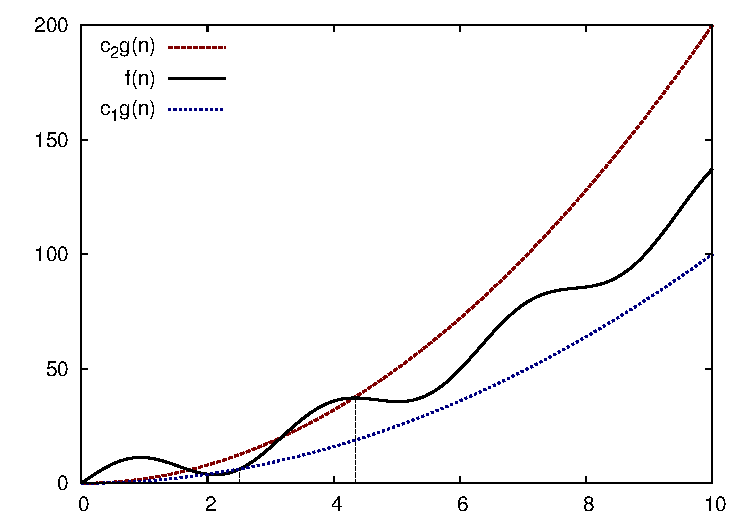
\includegraphics[width=.6\textwidth]{plot-3}
	\caption{Notazione asintotica \(\Theta\).}
	\label{fig:plot-3}
\end{figure}

\section{Complessità di un algoritmo e di un problema}

\begin{definition*}[complessità in tempo di un \alert{algoritmo}]
La più grande quantità di tempo richiesta \emph{per un input} di dimensione \(n\).
\end{definition*}
\begin{itemize}
	\item \(\Omicron(f(n))\): per tutti gli input, l'algoritmo costa al più \(f(n)\);
	\item \(\Omega(f(n))\): per tutti gli input, l'algoritmo costa almeno \(f(n)\);
	\item \(\Theta[f(n)]\): l'algoritmo richiede \(\Theta[f(n)]\) per tutti gli input.
\end{itemize}

\begin{definition*}[complessità in tempo di un \alert{problema computazionale}]
La complessità in tempo relativa \emph{a tutte le possibili soluzioni}.
\end{definition*}
\begin{itemize}
	\item \(\Omicron(f(n))\): complessità del miglior algoritmo che risolve il problema;
	\item \mbox{\(\Omega(f(n))\): dimostrare che nessun algoritmo può risolvere il problema in tempo inferiore a \(\Omega(f(n))\)};
	\item \(\Theta[f(n)]\): abbiamo trovato l'algoritmo ottimo.
\end{itemize}

\clearpage
\section{Esercizi}

\subsubsection*{Primo esercizio}

Iniziamo con degli esercizi banali che ci permetteranno di introdurre delle tecniche che utilizzeremo con le ricorrenze.
In particolare ci serviranno a renderci conto che non stiamo dimostrando equazioni, ma disequazioni.

\exercise{\( f(n) = 10 n^3 + 2 n^2 + 7 \overset{?}{=} \mathcal{O}(n^3) \)}

\textbf{Limite superiore}: Dobbiamo dimostrare che \( \exists c > 0, \exists m \geqslant 0: f(n) \bs{\leqslant} cn^3, \forall n \geqslant m\)
\[
\begin{WithArrows}
	f(n) &= 10 n^3 + 2 n^2 + 7 \Arrow[jump = 2]{\( \forall n \geqslant 1 \)} \\
	&\leqslant 10 n^3 + 2 n^{3} + 7 \\
	&\leqslant 10 n^3 + 2 n^3 + 7 n^3 \Arrow{sommiamo i termini} \\
	&= 19 n^3 \Arrow[tikz={text width=4cm}]{esiste una certa costante \(c\) per la quale \(f(n) \leqslant cn^3\) ?}\\
	&\overset{?}{\leqslant} cn^3 \Arrow{metto a confronto}\\
	19 n^3 &\leqslant cn^3 \Arrow{semplifico}\\
	19 \cancel{n^3} &\leqslant c\cancel{n^3}
\end{WithArrows}
\]

che è vera per ogni \(c \geqslant 19\) (abbiamo così trovato la costante moltiplicativa) e per ogni \(n \geqslant 1\) (introdotta nei calcoli), quindi \(m = 1\) (che deriva da \(\forall n \geqslant m\)).

\begin{figure}[H]\centering
	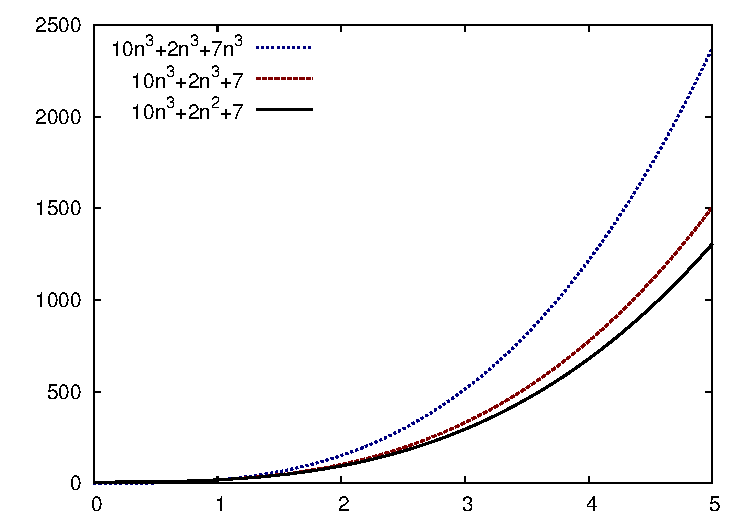
\includegraphics[width=.6\textwidth]{plot-0}
	\caption[]{Risoluzione grafica dell'esercizio.}
	\label{fig:plot-0}
\end{figure}

\begin{note}
In generale noi considereremo solo valori di \(n\) positivi, in quanto le funzioni di costo sono definite sull'insieme dei numeri naturali, non ha alcun senso definire una funzione di costo su una dimensione dell'input negativa.
\end{note}

\clearpage
\subsubsection*{Soluzione alternativa all'esercizio precedente}

Dato lo stesso esercizio posso esserci passaggi risolutivi diversi.
Risolviamo quindi l'esercizio precedente in modo diverso.

\exercise{\( f(n) = 10 n^3 + 2 n^2 + 7 \overset{?}{=} \mathcal{O}(n^3) \)}

\textbf{Limite superiore}: Dobbiamo dimostrare che \( \exists c > 0, \exists m \geqslant 0: f(n) \bs{\leqslant} cn^3, \forall n \geqslant m\)
\[
\begin{WithArrows}
	f(n) &= 10 n^3 + 2 n^2 + 7 \Arrow{\( \forall n \geqslant 1 \)} \\
	&\leqslant 10 n^3 + 2 n^{3} + 7 \Arrow{\(\forall n \geqslant \sqrt[3]{7}\)} \\
	&\leqslant 10 n^3 + 2 n^3 + n^3 \Arrow{sommiamo i termini} \\
	&= 13 n^3 \Arrow[tikz={text width=4cm}]{esiste una certa costante \(c\) per la quale \(f(n) \leqslant cn^3\) ?}\\
	&\overset{?}{\leqslant} cn^3 \Arrow{metto a confronto}\\
	13 n^3 &\leqslant cn^3 \Arrow{semplifico}\\
	13 \cancel{n^3} &\leqslant c\cancel{n^3}
\end{WithArrows}
\]
che è vera per ogni \( c \geqslant 13 \) e per ogni \( n \geqslant \sqrt[3]{7} \) (ad esempio con \(n=2\) abbiamo \(n^3 = 2^3 = 8\) che soddisfa la nostra condizione), quindi usiamo \( m = 2 \) (abbiamo semplificato, sarebbe \(m = \sqrt[3]{7}\), ma possiamo prendere un qualunque valore si trovi dopo \(n\) in modo totalmente arbitrario).

\begin{figure}[H]\centering
	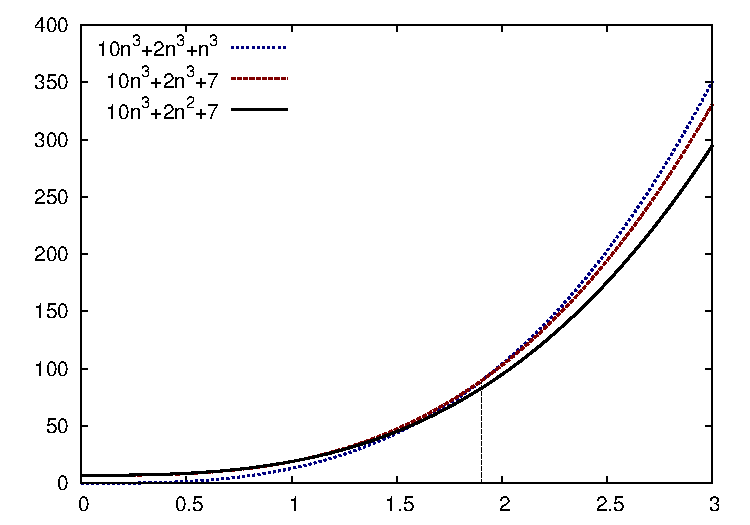
\includegraphics[width=.6\textwidth]{plot-0bis}
	\caption[]{Risoluzione grafica dell'esercizio.}
	\label{fig:plot-0bis}
\end{figure}

\clearpage
\subsubsection*{Secondo esercizio}

\exercise{\( f(n) = 3 n^2 + 7n \overset{?}{=} \Theta(n^2) \)}

\textbf{Limite inferiore}: Dobbiamo dimostrare che
\( \exists c_1 > 0, \exists m_1 \geqslant 0: \alert{f(n) \bs{\geqslant} c_1 n^2}, \forall n \geqslant m_1 \)
\[
\begin{WithArrows}
	f(n) &= 3 n^2 + 7 n \Arrow{\( \forall n \geqslant 0 \)} \\
	&\geqslant 3 n^2 \Arrow[tikz={text width=4cm}]{esiste una certa costante \(c\) per la quale \(f(n) \leqslant c_1 n^2\) ?}\\
	&\overset{?}{\geqslant} c_1 n^2 \Arrow{metto a confronto}\\
	3 n^2 &\leqslant c_1 n^2 \Arrow{semplifico}\\
	3 \cancel{n^2} &\leqslant c_1 \cancel{n^2}
\end{WithArrows}
\]
che è vera per ogni \( c_1 \bs{\leqslant} 3 \) e per ogni \( n \geqslant 0 \) (introdotta nei calcoli), quindi \( m_1 = 0 \).

\begin{note}
Abbiamo dimostrato quindi che \(f(n) = \Omega(n^2)\).
\end{note}

\textbf{Limite superiore}: Dobbiamo dimostrare che
\( \exists c_2 > 0, \exists m_2 \geqslant 0: \alert{f(n) \bs{\leqslant} c_2 n^2}, \forall n \geqslant m_2 \)
\[\begin{WithArrows}
	f(n) &= 3 n^2 + 2 n^2 + 7 n \Arrow{\( \forall n \geqslant 1 \)} \\
	&\leqslant 3 n^2 + 7 n^2 \Arrow{raccogliamo} \\
	&\leqslant 10 n^2 \Arrow[tikz={text width=4cm}]{esiste una certa costante \(c\) per la quale \(f(n) \leqslant c_2 n^2\) ?}\\
	&\overset{?}{\leqslant} c_2 n^2 \Arrow{metto a confronto}\\
	10 n^2 &\leqslant c_2 n^2 \Arrow{semplifico}\\
	10 \cancel{n^2} &\leqslant c_2 \cancel{n^2}
\end{WithArrows}\]
che è vera per ogni \( c_2 \bs{\geqslant} 10 \) e per ogni \( n \geqslant 1 \), %\\
quindi \( m_2 = 1 \).

\begin{note}
Abbiamo dimostrato quindi che \(f(n) = \mathcal{O}(n^2)\).
\end{note}

\textbf{Notazione \(\Theta\)}: \( \exists c_1 > 0, \exists c_2 > 0, \exists m \geqslant 0 \colon \alert{c_1 n^2 \bs{\leqslant} f(n) \bs{\leqslant} c_2 n^2}, \forall n \geqslant m \).

Con questi paramentri:
\begin{itemize}
	\item \(c_1 = 3\);
	\item \(c_1 = 10\);
	\item \(m = max\{m_1, m_2\} = max\{0, 1\} = 1\), ossia un valore dopo il quale la nostra proprietà è provata.
\end{itemize}

\begin{note}
Abbiamo dimostrato quindi che \(f(n) = \Theta(n^2)\).
\end{note}

\begin{figure}[H]\centering
	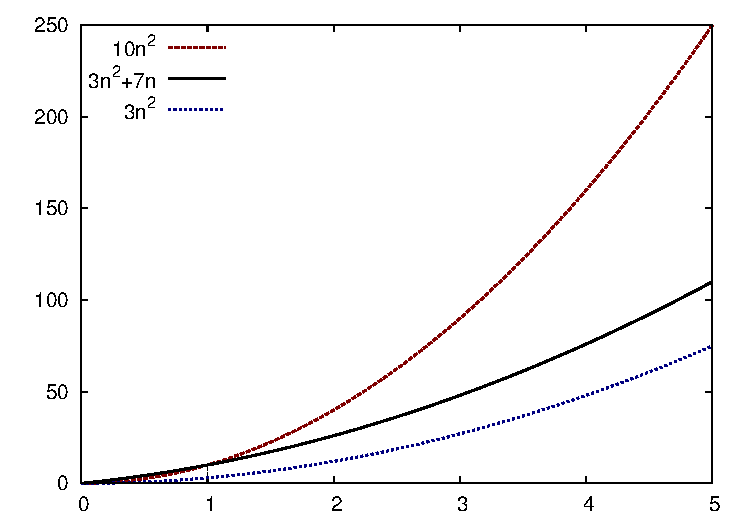
\includegraphics[width=.6\textwidth]{plot-1}
	\caption[]{Risoluzione grafica dell'esercizio.}
	\label{fig:plot-1}
\end{figure}

\clearpage
\section*{Errori comuni durante la risoluzione degli esercizi}

\subsubsection*{Dimostrare un limite superiore inesistente}

\exercise{\( f(n) = n^2 \overset{?}{=} \Omicron(n) \)}

\textbf{Limite superiore}: Dobbiamo dimostrare che \( \exists c > 0, \exists m \geqslant 0 \colon \alert{n^2 \bs{\geqslant} cn}, \forall n \geqslant m \).

Otteniamo che \(n^2 \leqslant cn \Leftrightarrow c \geqslant n\) (ad esempio con \(n=2\), \(2^2 \leqslant c \cdot 2 \Leftrightarrow c \geqslant 2\)), questo significa che \(c\) cresce con il crescere di \(n\), non possiamo quindi scegliere una \emph{costante} \(c\) che verifichi la proprietà.

\begin{figure}[H]\centering
	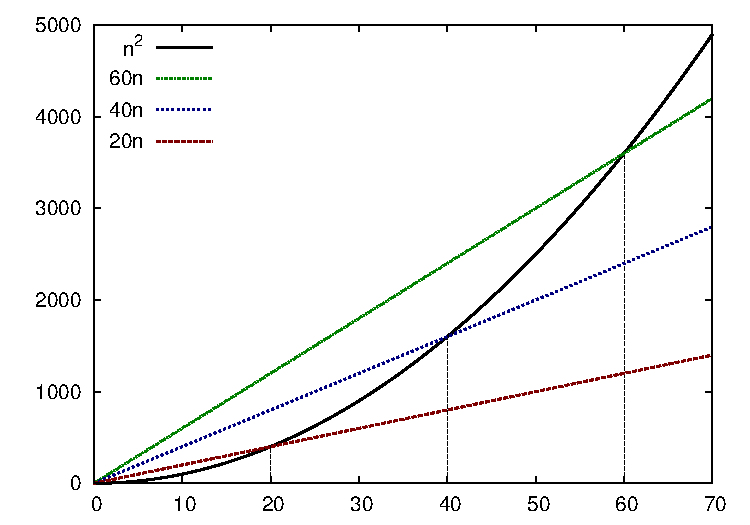
\includegraphics[width=.6\textwidth]{plot-nvsn2}
	\caption[]{Per qualunque fattore \(c\) scelto (ossia la pendenza della retta) la curva quadratica crescerà sempre più velocemente da un certo punto in poi.}
	\label{fig:plot-nvsn2}
\end{figure}

\subsubsection*{Dimostrare un limite inferiore inesistente}

\exercise{\( f(n) = n^2 \overset{?}{=} \Omega(n^3) \)}

\textbf{Limite inferiore}: Dobbiamo dimostrare che \(\exists c > 0, \exists m \geqslant 0, n^2 \geqslant cn^3, \forall n \geqslant m\).

Otteniamo che \(n^2 \geqslant cn^3 \Leftrightarrow c \leqslant \frac{1}{n}\) (ad esempio con \(n=2\), \(2^2 \geqslant c \cdot 2 \Leftrightarrow c \leqslant \frac{1}{2}\)), questo significa che \(c\) diminuisce al crescere di \(n\), non possiamo quindi scegliere una costante \(c\) che verifichi la proprietà.

\clearpage
\section{Complessità degli algoritmi e dei problemi a confronto}

In questa sezione ragioneremo su alcuni algoritmi risolutivi che ci sono stati insegnati, in alcuni casi si può migliorare la complessità, in altri è impossibile fare di meglio.

\begin{quote}
Qual è il rapporto fra un problema computazionale e l'algoritmo?
\end{quote}

\subsection{Moltiplicare numeri complessi}

La moltiplicazione fra numeri complessi avviene nel seguente modo: \((a + bi)(c + di) = [ac - db] + [ad + bc]i\).
Abbiamo in input \(a\), \(b\), \(c\), \(d\) e dobbiamo restituire in output \(ac - bd\) e \(ad + bc\).

Consideriamo un modello di calcolo dove la moltiplicazione costa \num{1} e le addizioni e sottrazioni costano \num{0.01}.
\begin{enumerate}
	\item Quanto costa l'algoritmo dettato dalla definizione?
	\item Riesci a fare meglio di così?
	\item Qual è il ruolo del modello di calcolo?
\end{enumerate}

L'algoritmo banale dettato dalla definizione costa \num{4.02}, in quanto bisogna fare 4 moltiplicazioni, 1 somma ed una sottrazione.

\subsubsection*{Soluzione di Gauss per la moltipicazione di numeri complessi}

La seguente è la soluzione di Gauss al problema, datata 1805.

Input: \(a\), \(b\), \(c\), \(d\), Output: \(A1 = ac - bd\), \(A2 = ad + bc\)
\let\oldtimes\times
\renewcommand\times{\mathcolor{red}{\bs{\oldtimes}}}
\let\oldplus\plus
\renewcommand\plus{\mathcolor{red}{\bs{\oldplus}}}
\let\oldminus\minus
\renewcommand\minus{\mathcolor{red}{\bs{\oldminus}}}
\[\begin{WithArrows}
m_1	&= a \times c \Arrow[tikz=-, jump=2, tikz=darker]{calcolo i valori intermedi} \\
m_2 &= b \times d \\
A_1 &= m_1 \minus m_2 \\
m_3	&= (a \plus b) \times (c \plus d) = ac + ad + bc + bd \Arrow{evito una moltiplicazione} \\
A_2	&= m_3 \minus m_1 \minus m_2 = ad + bc
\end{WithArrows}\]
\renewcommand\times{\oldtimes}
\renewcommand\plus{\oldplus}
\renewcommand\minus{\oldminus}

Il costo totale è \num{3.05}.

\begin{quote}
Si può fare ancora meglio di così?
Oppure è possibile dimostrare che non si può?
\end{quote}

\clearpage
\subsection{Sommare numeri binari}

\begin{note}
In questo caso usiamo il criterio del costo logaritmico.
\end{note}

L'algoritmo elementare della somma richiede di esaminare tutti gli \(n\) bit, il costo totale risulta \(cn\), dove \(c\) è il costo per sommare due bit e generare il riporto.

\begin{quote}
Esiste un metodo più efficiente?
\end{quote}

\`{E} dimostrabile per assurdo che \emph{non è possibile fare di meglio} di una soluzione lineare, poiché non è possibile sommare due numeri binari senza esaminare tutti gli \(n\) bit.

\subsection*{Limiti alla complessità di un problema}

\begin{definition*}[limite superiore, \(\mathcal{O}(f(n))\)]
Un problema ha complessità \(\mathcal{O}(f(n))\) \emph{se esiste almeno un algoritmo} che ha complessità \(\mathcal{O}(f(n))\).
\end{definition*}

\begin{note}
Il problema della somma dei numeri binari ha complessità \(\Omicron(n)\).
\end{note}

\begin{definition*}[limite inferiore, \(\Omega(f(n))\)]
Un problema ha complessità \(\Omega(f(n))\) \emph{se tutti i possibili algoritmi} che lo risolvono hanno complessità \(\Omega(f(n))\).
\end{definition*}

\begin{note}
Il problema della somma dei numeri binari ha complessità \(\Omega(n)\).
\end{note}

\subsection{Moltiplicare numeri binari}

L'algoritmo elementare del prodotto richiede di moltiplicare ogni bit con ogni altro bit, per un costo totale di \(c n^2\).

\begin{figure}[H]
	\centering
	\label{fig:mul}
	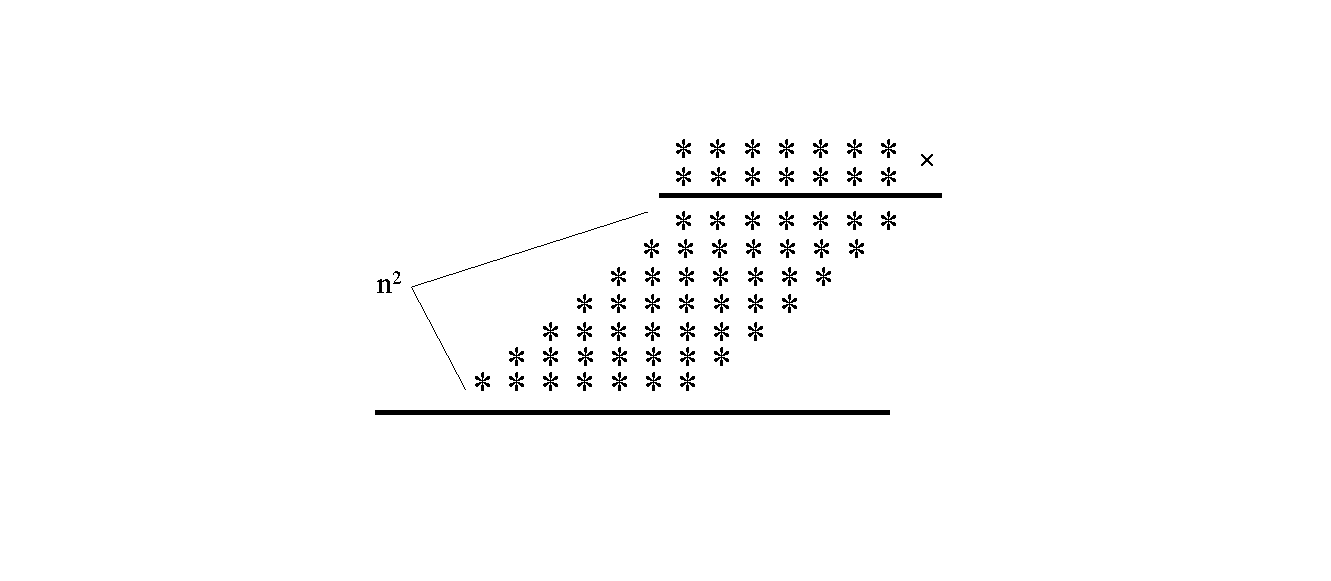
\includegraphics[width=.4\textwidth]{mul}
	\caption[]{Moltiplicazione di due numeri binari.}
\end{figure}

Si potrebbe concludere che il problema della moltiplicazione è molto più costoso del problema dell'addizione: ne è conferma la nostra esperienza.

\begin{note}
Per provare che il problema del prodotto è più costoso del problema della somma, dobbiamo provare che non esiste una soluzione in tempo lineare al problema del prodotto.
\end{note}

Abbiamo infatti erroneamente confrontato gli algoritmi, non i problemi!
Sappiamo solo che l'algoritmo della somma che ci hanno insegnato è più efficiente di quello della moltiplicazione.

Nel 1960, Kolmogorov enunciò che la moltiplicazione avesse limite inferiore pari a \(\Omega(n^2)\), una settimana dopo un suo studente Karatsuba riuscì a provare il contrario.
Osserviamo la sua soluzione.

\clearpage
\subsubsection*{Approccio divide-et-impera}

Karatsuba adottò un approccio divide-et-impera.

\begin{definition}[approccio divide-et-impera]
Si svolge in tre parti:
\begin{itemize}
	\item \textbf{Divide}: dividi il problema in sottoproblemi di dimensione inferiore;
	\item \textbf{Impera}: risolvi i sottoproblemi in maniera ricorsiva;
	\item (\textbf{Combina}): unisci le soluzioni dei sottoproblemi in modo da ottenere la risposta del problema principale.
\end{itemize}
\end{definition}
\[\begin{WithArrows}
X  &= a \cdot 2^{\nicefrac{n}{2}} + b \\
Y  &= c \cdot 2^{\nicefrac{n}{2}} + d \\
XY &= ac \cdot 2^n + (ad + bc) \cdot 2^{\nicefrac{n}{2}} + db
\end{WithArrows}\]

\begin{algorithm}[H]
\caption{Moltiplicazione di due numeri binari}

\BlankLine
% \tcp{moltiplica due numeri binari}
\prototype{\Array{\Bool} \pdi{\Array{\Bool} X, \Array{\Bool} Y, \Int n}}{
\params{X}[numero binario]
\params{Y}[numero binario]
\params{n}[numero di bit contenuti]

	\BlankLine
	\eIf{\(n \Equal 1\)}{
		\Return \(X[1] \cdot Y[1]\)\Comment*[l]{eseguo la moltiplicazione di due bit}
	}{
		spezza \(X\) in \(a\);\(b\) e \(Y\) in \(c\);\(d\)\;
		\Return \(\pdi{a, c, \nicefrac{n}{2}} \cdot 2^n + (\pdi{a, d, \nicefrac{n}{2}} + \pdi{b, c, \nicefrac{n}{2}}) \cdot 2^{\nicefrac{n}{2}} + \pdi{b, d, \nicefrac{n}{2}}\)\;
	}
}
\end{algorithm}

\paragraph{Complessità}
Moltiplicare per \(2^t\) è equivalente ad eseguire uno \foreign{shift} di \(t\) posizioni, in tempo lineare, quindi l'equazione di ricorrenza risultante è
\[
	T(n) =
	\begin{dcases}
		c_1                               & n = 1 \\
		4T(\nicefrac{n}{2}) + c_2 \cdot n & n > 1 \\
	\end{dcases}
	% = \mathcal{O}(n^2)
\]

\begin{note}
Non sappiamo ancora trattare questo genere di problemi, quindi facciamo solo degli accenni.
\end{note}

\paragraph{Analisi della ricorsione}
% (vedi figura) % TODO inserire immagine ricorsione
Al primo passo la chiamata ricorsiva avviene su una dimesione \(n\), al secondo passo vengono effettuate \(4\) chiamate ricorsive su una dimesione \(\nicefrac{n}{2}\), al terzo passo vengono effettuate \(4^2 = 16\) chiamate ricorsive su una dimesione \(\nicefrac{n}{2^2}\)\dots
al livello \(i\)-esimo vengono effettuate \(4^i\) chiamate ricorsive su una dimesione \(\nicefrac{n}{2^i}\).
Una volta arrivati al passo \(\log_2 n\) vengono effettuate \(4^{\log n}\) chiamate ricorsive su una dimesione pari al caso base \(T(1)\), per la proprietà dei logaritmi \(4^{\log n} = n^{\log 4} = n^2\), le dimensioni delle chiamate ricorsive vengono ridotte ad una semplice costante.
Possiamo quindi concludere che \(T(n) = \Omicron(n^2)\).

\clearpage
\subsubsection*{Moltiplicazione di Karatsuba}

\`{E} possibile ridurre ulteriormente la complessità.
\[\begin{WithArrows}
	A_1 &= a \times c \Arrow[jump=2, tikz=darker]{calcolo un valore intermedio} \\
	A_2 &= b \times d \\
	m   &= (a \plus b) \times (c \plus d) = ac + ad + bc + bd \Arrow{evito una moltiplicazione} \\
	A_3 &= m \minus A_1 \minus A_2 = ad + bc
\end{WithArrows}\]

\paragraph{Principio}
Effettuo un'unica moltiplicazione che mi permette di calcolare un valore intermedio che contiene la somma di tutte le combinazioni (\(m\)), e ricavo \(ad + bc\) tramite due sottrazioni (nello stesso modo in cui lavorava Gauss) evitando così una moltiplicazione.

\begin{algorithm}[H]
\caption{Moltiplicazione di Karatsuba}

\BlankLine
\prototype{\Array{\Bool} \karatsuba{\Array{\Bool} X, \Array{\Bool} Y, \Int n}}{

	\BlankLine
	\eIf{\(n \Equal 1\)}{
		\Return \(X[1] \cdot Y[1]\)\Comment*[l]{rimane invariato}
	}{
		spezza \(X\) in \(a\);\(b\) e \(Y\) in \(c\);\(d\)\;

		\BlankLine
		\Array{\Bool} \(A1 = \karatsuba{a, c, \nicefrac{n}{2}}\)\;
		\Array{\Bool} \(A3 = \karatsuba{b, d, \nicefrac{n}{2}}\)\;
		\Array{\Bool} \(m\) = \karatsuba{\(a + b\), \(c + d\), \(\nicefrac{n}{2}\)}\Comment*[l]{potrebbe essere \(\nicefrac{n}{2} + 1\)}
		\Array{\Bool} \(A2 = m - A1 - A3\)\Comment*[l]{ottengo A2 tramite sottrazione}

		\BlankLine
		\Return \(A1 \cdot 2^n + A2 \cdot 2^{\nicefrac{n}{2}} + A3\)\Comment*[l]{effettuo degli shift}
	}
}
\end{algorithm}

\paragraph{Complessità}
L'equazione di ricorrenza risultante è:
\[
	T(n) =
	\begin{dcases}
		c_1                               & n = 1 \\
		3T(\nicefrac{n}{2}) + c_2 \cdot n & n > 1 \\
	\end{dcases}
	% = \mathcal{O}(n^{1.58\dots})
\]

\paragraph{Analisi della ricorsione}
% TODO inserire immagine Ricorsione
Al primo passo la chiamata ricorsiva avviene su una dimesione \(n\), al secondo passo vengono effettuate \(3\) chiamate ricorsive su una dimesione \(\nicefrac{n}{2}\), al terzo passo vengono effettuate \(3^2 = 9\) chiamate ricorsive su una dimesione \(\nicefrac{n}{3^2}\)\dots
al livello \(i\)-esimo vengono effettuate \(3^i\) chiamate ricorsive su una dimesione \(\nicefrac{n}{2^i}\).
Una volta arrivati al passo \(\log_2 n\) vengono effettuate \(3^{\log n}\) chiamate ricorsive su una dimesione pari al caso base \(T(1)\), per la proprietà dei logaritmi \(3^{\log n} = n^{\log 3} = n^{1.58\dots}\).
Le dimensioni delle chiamate ricorsive vengono ridotte ad una semplice costante.
Possiamo quindi concludere che \(T(n) = \Omicron(n^{1.58\dots})\).

\begin{note}
L'algoritmo ingenuo (\foreign{na\"if}) non è sempre il migliore a meno che non sia possibile dimostrare il contrario.
\end{note}

Negli anni sono stati proposti diversi algoritmi, che il limite inferiore al problema della moltiplicazione sia \(\Omega(n \log n)\) è una congettura.
Una congettura è un'affermazione o un giudizio fondato sull'intuito, ritenuto probabilmente vero, ma non ancora rigorosamente dimostrato, cioè dunque relegato solamente a rango di ipotesi.

Nella GNU Multiple Precision Arithmetic Library vengono utilizzati diversi algoritmi al crescere di \(n\), il valore soglia per cui si predilige un algoritmo rispetto ad un altro dipende dal tipo di architettura.

\clearpage
\section{Algoritmi di ordinamento}

In questa lezione impareremo a capire quando è meglio utilizzare un algoritmo di ordinamento rispetto ad un altro.

In alcuni casi, gli algoritmi si comportano diversamente a seconda delle caratteristiche dell'input.
Conoscere in anticipo tali caratteristiche permette di scegliere l'algoritmo migliore in quella determinata situazione.

\section*{Tipologia di analisi}

Esistono tre tipi di analisi:
\begin{enumerate}
	\item analisi del \textbf{caso pessimo}: è la tipologia più importante, il tempo di esecuzione nel caso peggiore è il limite superiore al tempo di esecuzione per qualsiasi input. Per alcuni algoritmi il caso peggiore si verifica molto spesso (ad esempio nella ricerca di dati non presenti nel database);
	\item analisi del \textbf{caso medio}: è difficile da definire (cosa si intende per \enquote{medio} ?), dobbiamo avere una conoscenza pregressa sulle distribuzioni;
	\item analisi del \textbf{caso ottimo}: può avere senso se si conoscono informazioni particolari sull'input.
\end{enumerate}

\section*{Problema dell'ordinamento}

Data una sequenza \(A = a_1, a_2, \dots, a_n\) di \(n\) valori in input, il problema dell'ordinamento consiste nel restituire in output una sequenza \(B = b_1, b_2, \dots, b_n\) che sia una permutazione di \(A\), tale per cui \mbox{\(b_1 \leqslant b_2 \leqslant \dots \leqslant b_n\)} (ovvero che ci sia un ordinamento \emph{totale}).

Un approccio \enquote{demente} è quello di generare tutte le possibili permutazioni (complessità \(n!\)) fino a quando non se ne trova una ordinata.

\clearpage
\subsection{Selection sort}

Un approccio banale (\foreign{na\"if}) è quello di cercare il minimo e metterlo nella posizione corretta, riducendo il problema agli \(n-1\) valori rimanenti.

\begin{algorithm}[H]
	\caption{selectionSort}
	%&../preamble

\setcounter{section}{1}
% \setcounter{algocf}{5}

% arara: pdflatex: { synctex: no }
% arara: latexmk: { clean: partial }
\ifstandalone
\begin{document}
\begin{algorithm}[H]
\fi

\tcp{effettua l'ordinamento di un vettore}
\prototype{\selectionSort{\Array{\Item} A, \Int n}}{
	\From(\tcp*[h]{l'ultimo elemento è ordinato}){\Int \(i \Assign 1\) \DownTo \(n-1\)}{
		\Int \(j \Assign \minFunction{A, i, n}\)\Comment*[l]{ricerca il nuovo minimo}
		% \Swap{\(A[i]\)}{\(A[j]\)}\Comment*[l]{lo metto nella posizione corretta}
		\(A[i] \leftrightarrow A[j]\)\Comment*[l]{lo metto nella posizione corretta}
	}
}

\BlankLine
\tcp{cerca l'indice dell'elemento più piccolo}
\prototype{\Int \minFunction{\Array{\Item} A, \Int i, \Int j}}{

	\BlankLine
	\Int \(min \Assign i\) \Comment*[h]{posizione del minimo parziale}\;
	\From{\Int \(j \Assign i+1\) \DownTo \(n\)}{

		\BlankLine
		\If(\Comment*[h]{ho trovato un nuovo minimo}){\( A[j] < A[min] \)}{
			\(min \Assign j\) \Comment*[h]{nuovo minimo parziale}\;
		}
	}

	\BlankLine
	\Return \(min\)\Comment*[l]{restituisco l'indice dell'elemento più piccolo}
}
% \begin{algomathdisplay}
% 	\sum_{i=1}^{n-1} (n-1) = \sum_{i=1}^{n-1} i = \frac{n(n-1)}{2} = n^2 - \frac{n}{2} = \Theta(n^2)
% \end{algomathdisplay}
\ifstandalone
\end{algorithm}
\end{document}
\fi

\end{algorithm}

\begin{figure}[H]\centering
	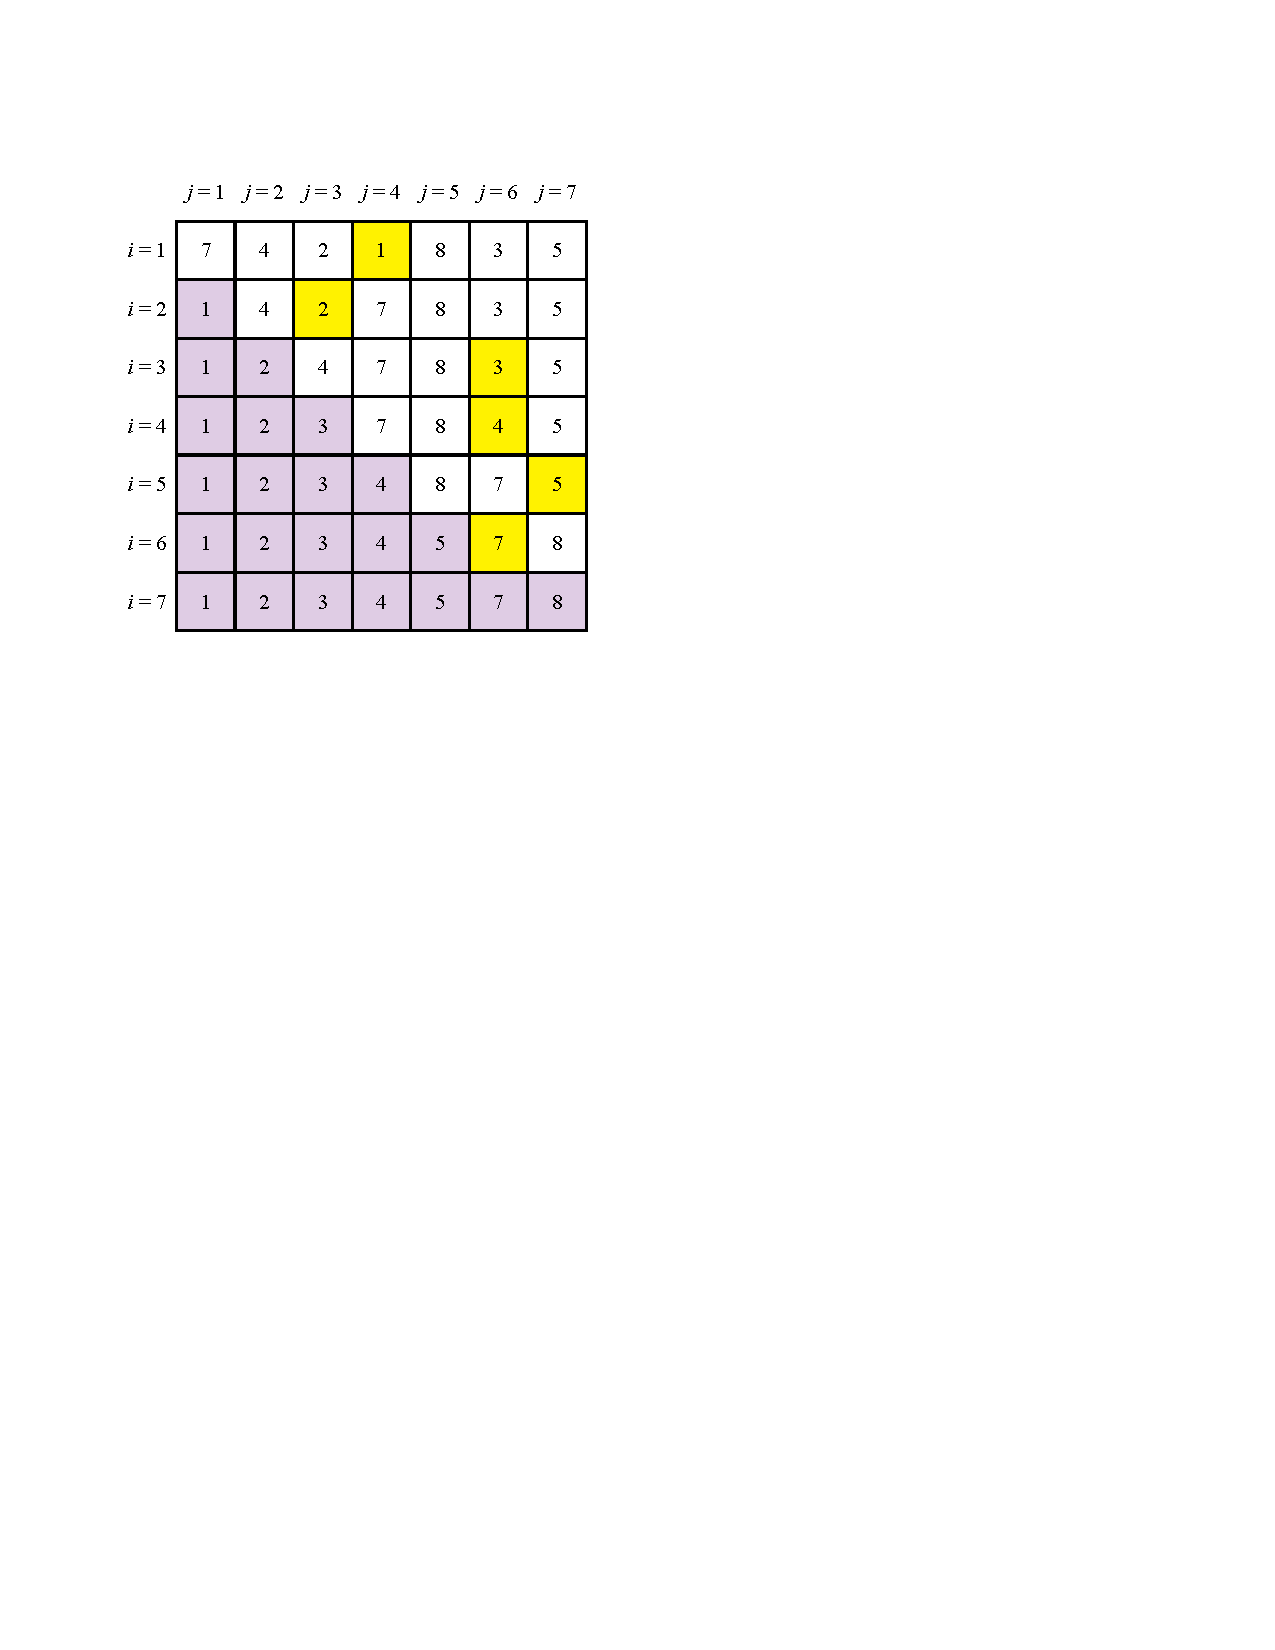
\includegraphics{selection}
	\caption[]{Funzinamento dell'algoritmo \selectionSort.}
\end{figure}

% TODO scrivere spiegazione selectionSort
% \paragraph{Spiegazione}
% Diamo per scontato che il primo elemento sia ordinato.

\begin{hint}
Provalo su carta!
Un algoritmo dev'essere provato per essere capito!
\end{hint}

\paragraph{Analisi della complessità}
Il ciclo effettua \(n\) chiamate della funzione \minFunction (una per ciascuna iterazione).
Ad ogni iterazione il vettore su cui viene calcolato il minimo risulta più piccolo di un elemento.
\[\begin{WithArrows}
	&\sum_{i=1}^{n-1} (n-1) \Arrow{\(10+9+\dots+1 \Leftrightarrow 1+2+\dots+10\)} \\
	&= \sum_{i=1}^{n-1} i \\
	&= \frac{n(n-1)}{2} \Arrow{svolgo i calcoli} \\
	&= n^2 - \frac{n}{2} \\
	&= \Theta(n^2)
\end{WithArrows}\]
Posso dire che è \(\Theta(n^2)\), e non solo che \(\Omega(n^2)\), perché indipendentemente dall'ordine iniziale ci metterà sempre lo stesso tempo.
In altre parole, il caso migliore, peggiore e medio coincidono.

\clearpage
\subsection{Insertion sort}

Un algoritmo che si basa sul principio di ordinamento di una \enquote{mano} di carte da gioco è il seguente:

\begin{algorithm}[H]
	\caption{insertionSort}
	%&../preamble

% arara: pdflatex: { synctex: no }
% arara: latexmk: { clean: partial }
\ifstandalone
\begin{document}
\begin{algorithm}[H]
\fi

% \tcp{efficiente per ordinare piccoli insiemi di elementi}
\tcp{effettua l'ordinamento di un vettore}
\prototype{\insertionSort{\Item{} A, \Int n}}{

	\BlankLine
	\From(\Comment*[h]{il 1\textsuperscript{o} elemento verrà ordinato in seguito}){\Int \(i=2\) \DownTo \(n\)}{

		\BlankLine
		\Item \(temp \Assign A[i]\) \Comment*[h]{elemento da ordinare}\;
		\Int \(j \Assign i\)\;

		\BlankLine
		\While{\(j > 1\) \And \(A[j-1] > temp\)}{
			\(A[j] \Assign A[j-1]\) \Comment*[h]{copio l'elemento}\;
			\Decrement{j} \Comment*[h]{mi sposto}\;
		}

		\BlankLine
		\(A[j] \Assign temp\)\;
	}
}
% \tcp{vettore già ordinato: \(\Omega(n)\)}
% \tcp{vettore decrescente: \(\Omicron(n^2)\)}
% \tcp{in media \(\Omicron(n^2)\)}
\ifstandalone
\end{algorithm}
\end{document}
\fi

\end{algorithm}

% TODO scrivere spiegazione insertionSort
% \paragraph{Spiegazione}
% Diamo per scontato che il primo elemento sia ordinato.

Questo è un algoritmo molto efficiente per ordinare piccoli insiemi di elementi.

\paragraph{Analisi della complessità}
Il \emph{costo di esecuzione} di questo algoritmo non \emph{dipende} solo dalla dimensione del vettore, ma anche \emph{dalla distribuzione dei dati in ingresso}.
Nel caso in cui il vettore sia già \emph{ordinato} il costo è \(\Omicron(n)\), in quanto non si entra mai nel secondo ciclo dato che la condizione risulta falsa.
Nel caso in cui il vettore sia \emph{ordinato in ordine inverso} è \(\Omega(n^2)\).
In media (informalmente) possiamo assumere che metà dei valori sia ordinata rispetto la loro disposizione finale e quindi metà di loro dovrà fare \(n\) passi per arrivare alla destinazione per una complessità di \(n \cdot \nicefrac{n}{2} = \Omicron(n^2)\).

Infine quando sappiamo che i valori sono quasi ordinati o che \(n\) è molto piccolo (nell'ordine di 16 o 32 elementi) allora questo algoritmo risulta efficiente.

\clearpage
\subsection{Merge sort}

MergeSort è basato sulla tecnica divide-et-impera vista in precendenza.
Ma come la utilizza?

\begin{definition}[approccio divide-et-impera di MergeSort]
Si svolge in tre parti:
\begin{itemize}
	\item \textbf{divide}: spezza il vettore di \(n\) elementi in 2 sottovettori di \(\frac n 2\) elementi;
	\item \textbf{impera}: chiama \mergeSort ricorsivamente sui due sottovettori (ottenendo due metà ordinate);
	\item (\textbf{combina}): unisce (da questo deriva \foreign{merge}) le due sequenze ordinate.
\end{itemize}
\end{definition}

L'idea alla base di questo algoritmo sfrutta il fatto che è possibile \emph{unire due sottovettori ordinati} in un vettore ordinato \emph{in tempo lineare}.

\begin{algorithm}[H]
	\caption{mergeSort}
	%&../preamble

% arara: pdflatex: { synctex: no }
% arara: latexmk: { clean: partial }
\ifstandalone
\begin{document}
\begin{algorithm}[H]
\fi

\BlankLine
\tcp{ordina i sottovettori}
\prototype{\mergeSort{\Item{} \(A\), \Int \(primo\), \Int \(ultimo\)}}{

	\BlankLine
	\If(\Comment*[h]{devono esistere almeno due elementi}){\(primo < ultimo\)}{
		\Int \(mezzo \Assign \floor{\frac{primo + ultimo}{2}}\)\;
		\mergeSort{\(A\), \(primo\), \(mezzo\)}\;
		\mergeSort{\(A\), \(mezzo+1\), \(ultimo\)}\;
		\merge{\(A\), \(primo\), \(ultimo\), \(mezzo\)}\Comment*[l]{unisce le soluzioni}\;
	}
}

\ifstandalone
\end{algorithm}
\end{document}
\fi

% \BlankLine
% \BlankLine
% Equazione di ricorrenza:
% \[
% 	T =
% 	\begin{dcases}
% 		\Theta(1) & n = 1\\
% 		\T*{\nicefrac{n}{2}} + \T*{\nicefrac{n}{2}} + \Theta(n) & n > 1 \\
% 	\end{dcases}
% 	=
% 	\begin{dcases}
% 		c & n = 1\\
% 		2\T{\nicefrac{n}{2}} + dn & n > 1\\
% 	\end{dcases}
% \]
%
% \BlankLine
% Analisi per livelli:
% \[
% \Omicron \left( \sum_{i=0}^{k} \Ccancel{2^i} \frac{n}{\Ccancel{2^i}} \right) = \Omicron \left( \sum_{i=0}^{k} n \right) = \Omicron(k \cdot n) = \Omicron(n \log n)
% \]
% %
% Teorema dell'esperto:
%
% \begin{minipage}[t]{.4\linewidth}
% \begin{align*}
% 		\alpha &= \log_2 2 = 1 \\
% 		\beta  &= 1 \\
% 		\alpha &= \beta \\
% \end{align*}
% \end{minipage}
% \begin{minipage}[t]{.4\linewidth}
% \begin{align*}
% 	T &= \Omicron(n^{\alpha} \log n) \\
% 	  &= \Omicron(n \log n) \\
% \end{align*}
% \end{minipage}

	%&../preamble

% arara: pdflatex: { synctex: no }
% arara: latexmk: { clean: partial }
\ifstandalone
\begin{document}
\begin{algorithm}[H]
\fi

\BlankLine
\tcp{effettua l'ordinamento dei sotto-vettori}
\prototype{\merge{\Item \(A\), \Int \(primo\), \Int \(ultimo\), \Int \(mezzo\)}}{
	\Int \(i\), \(j\), \(k\), \(h\)\;

	\BlankLine
	\tcp{inizializzo i puntatori}
	\(i \Assign primo\)\;
	\(j \Assign mezzo\)\;
	\(k \Assign primo\)\tcp*[l]{\(k\): indica la prossima posizione di scrittura}

	\BlankLine
	% \tcp{}
	\While{\(i \leqslant mezzo\) \And \(j \leqslant ultimo\)}{

		\BlankLine
		\tcp{B è il vettore di appoggio in cui memorizzo la porzione di vettore già ordinata}
		\eIf{\(A[i] \leqslant A[j]\)}{
			\tcp{l'elemento è gia ordinato}
			\(B[k] \Assign A[i]\)\;
			\Increment{i}\;
		}{
			\(B[k] \Assign A[j]\)\;
			\Increment{j}\;
		}

		\BlankLine
		\tcp{\emph{in entrambi i casi} ho inserito un valore}
		\Increment{k}\;
	}

	\BlankLine
	\tcp{se uno dei due vettori finisce ricopio la parte ordinata alla fine del vettore d'appoggio}
	\(j \Assign ultimo\)\;
	\From{\(h \Assign mezzo\) \DownTo \(i\)}{
		\(A[j] \Assign A[h]\)\;
		\Decrement{j}\;
	}

	\BlankLine
	\tcp{ricopio il vettore d'appoggio del vettore originale}
	\From{\(j \Assign primo\) \DownTo \(k-1\)}{
		\(A[j] \Assign B[j]\)\;
	}
}

\ifstandalone
\end{algorithm}
\end{document}
\fi

\end{algorithm}

% TODO scrivere spiegazione mergeSort
% \paragraph{Spiegazione}
% Quando un'array diventa vuoto, copia tutti i valori dall'array rimanente nell'array ordinato.

\clearpage
\paragraph{Analisi della complessità}
Assumiamo (per semplicità) che \(n = 2^k\) (ovvero che l'altezza dell'albero di suddivisioni sia esattamente \(k = \log_2 n\)) e che tutti i sottovettori abbiano dimensioni che sono potenze esatte di 2.
L'equazione di ricorrenza risultante è la seguente:
\begin{align*}
	T &=
	\begin{dcases}
		\Theta(1) & n = 1\\
		\T*{\nicefrac{n}{2}} + \T*{\nicefrac{n}{2}} + \Theta(n) & n > 1 \\
	\end{dcases}\\
	&=
	\begin{dcases}
		c & n = 1\\
		2\T{\nicefrac{n}{2}} + dn & n > 1\\
	\end{dcases}\\
\end{align*}
Qual è il costo computazionale di \mergeSort?

\begin{figure}[H]\centering
	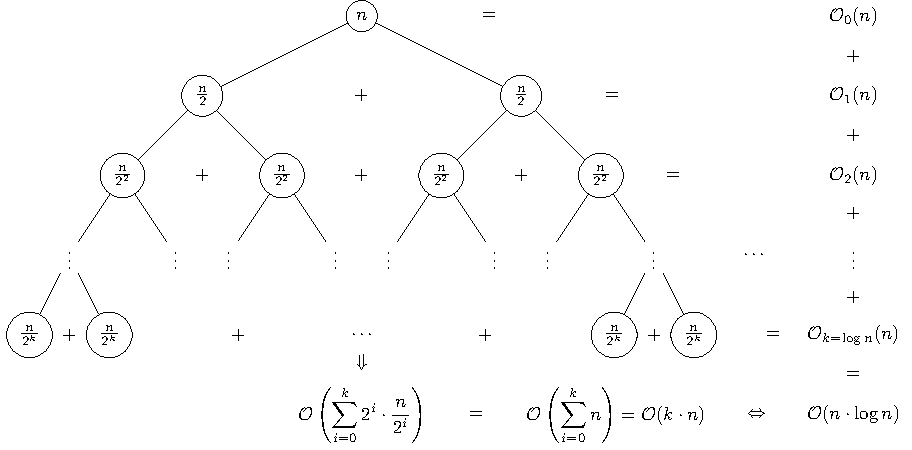
\includegraphics{mergesort-recursion}
	\caption[]{Analisi per livelli del costo di \mergeSort}
\end{figure}

L'analisi per livelli è la seguente:
\[\begin{WithArrows}
	&\Omicron \left( \sum_{i=0}^{k} \Ccancel{2^i} \frac{n}{\Ccancel{2^i}} \right) \Arrow{semplifico}\\
	&= \Omicron \left( \sum_{i=0}^{k} n \right) \Arrow{equivalente}\\
	&= \Omicron((k+1) \cdot n) \Arrow{\(k+1\) elementi, semplico perché è una costante}\\
	&= \Omicron(k \cdot n) \Arrow{\(k = \log n\)}\\
	&= \Omicron(n \log n)
\end{WithArrows}\]

\(\Omicron(n \log n)\) è asintoticamente migliore di \(\Omicron(n^2)\).
Questo algoritmo è preferibile --- per grandi dimensioni di \(n\) --- al \selectionSort e all'\insertionSort.

% NOTE fra dice che è abbastanza inutile 😞
% \section{Conclusioni}
%
% Abbiamo visto tre algoritmi di ordinamento:
% \begin{itemize}
% 	\item \selectionSort
% 	\item \insertionSort
% 	\item \mergeSort
% \end{itemize}
% Nell'ultima lezione vedremo molti altri algoritmi di ordinamento.
\ifsubfile
\end{document}
\fi

	%&../settings/preamble.main

\ifsubfile
\usepackage[newfloat, cachedir=_minted-cache, outputdir=../build]{minted}
\usepackage{../libraries/set-minted}

\pagestyle{plain}
\setcounter{chapter}{2}

% arara: pdflatex: { options: ["--output-directory=../build"], shell: yes, draft: yes, synctex: no }
% arara: pdflatex: { options: ["--output-directory=../build"], shell: yes, synctex: no }
\begin{document}
\fi
\chapter{Analisi delle funzioni di costo}

Abbiamo concluso la prima parte delle lezioni che ci introduceva alle equazioni di ricorrenza: ora andremo a capire i fondamenti matematici che ci permetteranno di analizzarne una famiglia più grande.

% NOTE ripasso della notazione asintotica e della complessità degli algoritmi e dei problemi.
\section{Proprietà della notazione asintotica}

\subsection{Regola generale}

\begin{theorem}[regola generale]
\(f(n) = a_k n^k + a_{k-1} n^{k-1} + \ldots a_1 n + a_0, a_k >0 \Rightarrow f(n) = \Theta(n^k)\)
\end{theorem}

\begin{proof}
\textbf{Limite superiore}: \(\exists c>0, \exists m \geqslant 0: f(n) \leqslant cn^k, \forall n \geqslant m\)

\[\begin{WithArrows}
f(n) &= a_k n^k + a_{k-1} n^{k-1} + \ldots + a_1 n + a_0 \Arrow{\(a_k > 0\) per def., rendo gli altri positivi}\\
	 &\leqslant a_k n^k + \abs{a_{k-1}} n^{k-1} +  \ldots  + \abs{a_1} n + \abs{a_0} \Arrow{\(\forall n \geqslant 1\), elevo tutte le potenze a \(k\)} \\
	 &\leqslant a_k n^k + \abs{a_{k-1}} n^k +  \ldots  + \abs{a_1} n^k + \abs{a_0} n^k \Arrow{raccolgo \(n^k\)}\\
	 &= (a_k + \abs{a_{k-1}}  +  \ldots  + \abs{a_1} + \abs{a_0})\, n^k \Arrow{esiste una costante \(c\)\\che rende la disequazione vera?} \\
	 &\stackrel{?}{\leqslant} cn^k
\end{WithArrows}\]
che è vera per \(c \geqslant (\abs{a_k} + \abs{a_{k-1}} + \ldots + \abs{a_1} + \abs{a_0} )\) (il coefficiente) e per \(m = 1\).
\end{proof}

\begin{proof}
\textbf{Limite inferiore}: \(\exists d>0, \exists m \geqslant 0: f(n) \geqslant d n^k, \forall n \geqslant m\)
\[\begin{WithArrows}
	f(n) &= a_k n^k + a_{k-1} n^{k-1} + \ldots + a_1 n + a_0 \Arrow[tikz={text width=4cm}]{normalizzo aggiungendo un segno negativo}\\
	&\geqslant a_kn^k - \abs{a_{k-1}} n^{k-1} - \ldots  - \abs{a_1} n - \abs{a_0} \Arrow{\(\forall n \geqslant 1\), elevo alla \(k-1\)}\\
	&\geqslant a_kn^k - \abs{a_{k-1}} n^{k-1} - \ldots  - \abs{a_1} n^{k-1} - \abs{a_0} n^{k-1} \\
	&\stackrel{?}{\geqslant} d n^k
\end{WithArrows}\]
L'ultima equazione è vera se:
\[
d \leqslant a_k - \frac{\abs{a_{k-1}}}{n} - \frac{\abs{a_{k-2}}}{n} -\ldots - \frac{\abs{a_1}}{n} - \frac{\abs{a_0}}{n} > 0
\iff
n > \frac{\abs{a_{k-1}} + \ldots + \abs{a_0}}{a_k} = m\qedhere
\]
% Costituito da una componente positiva (\(a_k\)) e da una componente negativa che per valori crescenti di \(n\) tende a \(0\).
\end{proof}
Abbiamo dimostrato sia il limite superiore che quello inferiore, possiamo affermare che è un \(\Theta\).

Ad esempio \(17n^3 - 47n^2 + 123n + 17 = \Theta(n^3)\).
Oppure \(2n^3 + 7 = \Theta(n^2)\).

\subsection{Funzioni di costo particolari}

La complessità di \(f(n) = 5\) è pari a \(\Theta(1)\), questa classe di complessità rappresenta quegli algoritmi che sono così ben congegnati che indipendentemente dalla dimensione dell'input impiegano un tempo costante a risolvere il problema.
Ad esempio richiedere il minimo in un vettore ordinato.

Dimostriamolo.
\begin{align*}
f(n) &= 5 \geqslant c_1 n^0 \Rightarrow c_1 \leqslant 5 \\
f(n) &= 5 \leqslant c_2 n^0 \Rightarrow c_2 \geqslant 5 \\
f(n) &= \Theta(n^0) = \Theta(1) \\
\end{align*}

La complessità di \(f(n) = 5 + \sin(n)\) è pari a \(\Theta(1)\), in quanto \(\sin(n)\) oscilla fra \(1\) e \(-1\).

\begin{figure}[H]\centering
	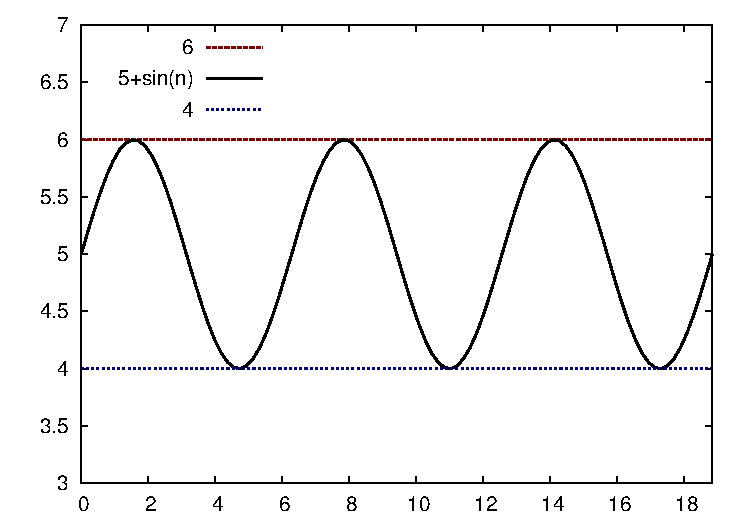
\includegraphics[width=.6\textwidth]{plot-2}
	\caption[]{\(\sin(n)\) oscilla fra \(1\) e \(-1\).}
	\label{fig:plot-2}
\end{figure}


\subsection{Proprietà delle notazioni}

\begin{theorem}[dualità]
Se \(f(n)\) è limitata superiormente da \(g(n)\), allora \(g(n)\) è limitata inferiormente da \(f(n)\).
\[ f(n) = \mathcal{O}(g(n)) \Leftrightarrow g(n) = \Omega(f(n)) \]
\end{theorem}
La dimostrazione avviene tramite passaggi algebrici.
\begin{proof}
\[\begin{WithArrows}
	f(n) = \mathcal{O}(g(n)) %
	&\Leftrightarrow f(n) \leqslant \bs{c}\ g(n), \forall n \geqslant m %
	\Arrow{ribalto la disequazione, \(c>0\)} \\
	&\Leftrightarrow g(n) > \bs{\frac{1}{c}}\: f(n), \forall n \geqslant m %
	\Arrow{rinomino \(\frac{1}{c}\) a \(c'\)} \\
	&\Leftrightarrow g(n) > \bs{c'}\, f(n), \forall n \geqslant m, c' = \frac{1}{c} %
	\Arrow{passo alla notazione dei quantificatori} \\
	&\Leftrightarrow g(n) = \Omega(f(n))
\end{WithArrows}\]
\end{proof}

\begin{theorem}[eliminazione delle costanti]
\[\begin{WithArrows}
f(n) = \Omicron(g(n)) \Leftrightarrow af(n) = \Omicron(g(n)), \forall a > 0 \\
f(n) = \Omega(g(n)) \Leftrightarrow af(n) = \Omega(g(n)), \forall a > 0
\end{WithArrows}\]
\end{theorem}
La dimostrazione avviene sempre tramite semplici passaggi algebrici.
\begin{proof}
\[\begin{WithArrows}
f(n) = \Omicron(g(n)) &\Leftrightarrow f(n) \leqslant c\,g(n), \forall n \geqslant m \Arrow{Introduco una costante \(a\)}\\
	  &\Leftrightarrow f(n) \leqslant ac\,g(n), \forall n \geqslant m, \forall a \geqslant 0 \Arrow{raccolgo \(ac\) sotto un'unica costante \(c'\)}\\
	  &\Leftrightarrow f(n) \leqslant c'g(n), \forall n \geqslant m, c' = ac > 0 \Arrow{per definizione}\\
	  &\Leftrightarrow a f(n) = \Omicron(g(n))
\end{WithArrows}\]
\end{proof}

Ad esempio \(2 \log n = \Theta(\log n)\), ignoriamo quindi le costanti numeriche.

\begin{theorem}[sommatoria, sequenza di algoritmi]
	\begin{align*}
	&
	\begin{dcases}
	f_1(n) = \Omicron(g_1(n)) \\
	f_2(n) = \Omicron(g_2(n)) \\
	\end{dcases}
	\Rightarrow f_1(n) + f_2(n) = \Omicron(\maxFunction(g_1(n),g_2(n)))\\
	&
	\begin{dcases}
	f_1(n) = \Omega(g_1(n)) \\
	f_2(n) = \Omega(g_2(n)) \\
	\end{dcases}
	\Rightarrow f_1(n) + f_2(n) = \Omega(\maxFunction(g_1(n),g_2(n)))\\
	\end{align*}
\end{theorem}
\begin{proof}
\[\begin{WithArrows}
f_1 (n) = \Omicron(g_1 (n)) \land f_2 n = \Omicron(g_2(n)) &\Rightarrow \Arrow{per definizione}\\
f_1 (n) \leqslant c_1 g_1 (n) \land f_2 (n) \leqslant c_2 g_2 (n) &\Rightarrow \Arrow[jump=2]{raccolgo}\\
f_1 (n) + f_2 (n) \leqslant c_1 g_1 (n) + c_2 g_2 (n) &\Rightarrow\\
f_1 (n) + f_2 (n) \leqslant \maxFunction\{c_1, c_2\}(2 \cdot \maxFunction(g_1(n), g_2(n)) &\Rightarrow \Arrow{per definizione}\\
f_1 (n) + f_2 (n) = \Omicron(g_1(n) + g_2(n))
\end{WithArrows}\]
\end{proof}

Ad esempio se ripeto due volte un algoritmo lineare, l'algoritmo risultante sarà comunque lineare.
Mentre se ho un algoritmo lineare ed un algoritmo quadratico, la complessità risultante è una combinazione delle due, il limite superiore della complessità totale sarà quindi quadratica.

\begin{theorem}[cicli annidati]
Se \(f_1(n)\) viene ripetuto \(f_2(n)\) volte, allora \(f_1(n) \cdot f_2(n)\) è limitato superiormente dal prodotto delle complessità e limitato inferiormente dal prodotto delle complessità.
\begin{align*}
	&
	\begin{dcases}
	f_1(n) = \Omicron(g_1(n)) \\
	f_2(n) = \Omicron(g_2(n)) \\
	\end{dcases}
	\Rightarrow f_1(n) \cdot f_2(n) = \Omicron(g_1(n) \cdot g_2(n))\\
	&
	\begin{dcases}
	f_1(n) = \Omega(g_1(n)) \\
	f_2(n) = \Omega(g_2(n)) \\
	\end{dcases}
	\Rightarrow f_1(n) \cdot f_2(n) = \Omega(g_1(n) \cdot g_2(n))\\
\end{align*}
\end{theorem}
La dimostrazione è molto semplice.
\begin{proof}
\[\begin{WithArrows}
f_1 (n) = \Omicron(g_1 (n)) \land f_2 n = \Omicron(g_2(n)) &\Rightarrow \Arrow{per definizione}\\
f_1 (n) \leqslant c_1 g_1 (n) \land f_2 (n) \leqslant c_2 g_2 (n) &\Rightarrow \Arrow{raccolgo, \(c_1 c_2 > 0\)}\\
f_1 (n) \cdot f_2 (n) \leqslant c_1 c_2 g_1(n) g_2(n)
\end{WithArrows}\]
\end{proof}

Ad esempio, se ripeto \(n\) volte un algoritmo di costo \(\log n\), l'algoritmo complessivo avrà un costo di \(n \log n\).

\begin{theorem}[simmetria]
Se \(f(n)\) è limitata superiormente ed inferiormente da \(g(n)\), allora anche \(g(n)\) è limitata inferiormente e superiormente da \(f(n)\).
	\[ f(n) = \Theta(g(n)) \Leftrightarrow g(n) = \Theta(f(n)) \]
\end{theorem}

Vuol dire semplicemente che \(2n^2 + 7 = \Theta(n^2) \Leftrightarrow n^2 = \Theta(2n^2 + 7)\).

La dimostrazione avviene tramite la proprietà di dualità:
\begin{proof}
\[\begin{WithArrows}
f(n) = \Theta(g(n)) &\quad\Rightarrow\quad f(n) = \Omicron(g(n)) \quad\Rightarrow\quad g(n) = \Omega(f(n)) \\
f(n) = \Theta(g(n)) &\quad\Rightarrow\quad f(n) = \Omega(g(n)) \quad\Rightarrow\quad g(n) = \Omicron(f(n))
\end{WithArrows}\]
\end{proof}

\begin{theorem}[transitività]
Se \(f(n)\) è limitata superiormente da \(g(n)\), e \(g(n)\) è limitata superiormente da \(h(n)\), allora \(f(n)\) è limitata superiormente da \(h(n)\).
\[
\begin{dcases}
f(n) = \mathcal{O}(g(n)) \\
g(n) = \mathcal{O}(h(n)) \\
\end{dcases}
\Rightarrow f(n) = \Omicron(h(n))
\]
\end{theorem}
La dimostrazione è banale:
\begin{proof}
\[\begin{WithArrows}
	f(n) = \mathcal{O}(g(n)) \land g(n) = \mathcal{O}(h(n)) &\Rightarrow %
	\Arrow{applico la definizione} \\
	f(n) \leqslant c_1 g(n) \land g(n) \leqslant c_2 h(n) &\Rightarrow %
	\Arrow{sostituisco \(g(n)\) con \(c_2 h(n)\)} \\
	f(n) \leqslant c_1 c_2 h(n) &\Rightarrow %
	\Arrow{\(c_1 c_2 > 0\), elimino la costante} \\
	f(n) = \mathcal{O}(h(n))
\end{WithArrows}\]
\end{proof}

\subsection*{Altre funzioni di costo}

Vogliamo provare che \fbox{\(\log n = \Omicron(n)\)}

Dimostriamo per induzione che \(\exists c > 0, \exists m \geqslant 0\,\colon \log n \leqslant cn, \forall n \geqslant m\).

\begin{itemize}
	\item \textbf{caso base} \((n=1)\):
	\[\begin{WithArrows}
	\log n &\leqslant cn \Arrow{\(n = 1\)}\\
	\log 1 &\leqslant c \cdot 1 \Arrow{semplifico}\\
	0 &\leqslant c
	\end{WithArrows}\]
	\item \textbf{ipotesi induttiva}: \(\log k \leqslant ck, \forall k \leqslant n\)
	\item \textbf{passo induttivo} dimostriamo la proprietà per \(n+1\):
	\[\begin{WithArrows}
	\log(n+1) \leqslant \log(n+n) &= \log2n \quad \forall n \geqslant 1 \Arrow{\(\log ab = \log a + \log b\)}\\
	&= \log 2 + \log n \Arrow{\(\log_2 2 = 1\)}\\
	&= 1 + \log n \Arrow{per ipotesi induttiva}\\
	&\leqslant 1 + cn \Arrow{obiettivo}\\
	&\overset{?}{\leqslant} c(n+1) \Arrow{metto a confronto}\\
	1 + cn &\leqslant c(n+1) \Arrow{moltiplico}\\
	1 + \Ccancel{cn} &\leqslant \Ccancel{cn} + c \Arrow{semplifico}\\
	1 &\leqslant c
	\end{WithArrows}\]
\end{itemize}

\subsection*{Classificazione delle funzioni}

\`{E} possibile trarre un ordinamento dalle principali espressioni, estendendo le relazioni che abbiamo dimostrato fino ad ora.
Per ogni \(r < s, h < k, a < b\):
\[
\Omicron(1)
\subset
\Omicron(\log^r n)
\subset
\Omicron(\log^s n)
\subset
\Omicron(n^h)
\subset
\Omicron(n^h \log^r n)
\subset
\Omicron(n^h \log^s n)
\subset
\Omicron(n^k)
\subset
\Omicron(a^n)
\subset
\Omicron(b^n)
\]

Ricordati che \(\log^r(n) = {(\log n)}^r\).
Non è detto che gli esponenti siano interi.
\(\sqrt[1000]{n}\) cresce più velocemente di \(\log^2 n\).
\(n\) cresce meno velocemente di \(n \log n\), il quale a sua volta cresce meno velocemente di \(n \log^2 n\).

\clearpage
\section{Analisi per livelli}

Nell'analisi per livelli (o dell'albero di ricorsione) andiamo sostanzialmente a \enquote{srotolare} la ricorrenza in un albero, i cui nodi rappresentano i costi dei vari livelli della ricorsione.

\subsection{Esempi di analisi per livelli}

\subsubsection*{Analisi per livelli dell'algoritmo della ricerca binaria}

Equazione di ricorrenza della ricerca binaria:
\[
	T(n) =
	\begin{dcases}
		T(\nicefrac{n}{2}) + b & n > 1 \\
		1 & n \leq 1 \\
	\end{dcases}
\]

Assumiamo per semplicità che \(n = 2^k\), ovvero che \(k = \log n\).
\`{E} possibile quindi risolvere questa ricorrenza nel seguente modo:
\[\begin{WithArrows}
T(n) &= b + T(\frac{n}{2}) \Arrow{\(T\left(\frac{n}{2} \cdot \frac{1}{2} \right) + b\)}\\
	 &= b + b + T(\frac{n}{4}) \Arrow{\(T\left(\frac{n}{4} \cdot \frac{1}{2} \right) + b\)}\\
	 &= b + b + b + T(\frac{n}{8}) \Arrow[jump=2]{svolgo \(\log n\) operazioni}\\
	 &\phantom{= b + b + b}\vdots\\
	 &= \underbracket[0.01mm]{b + b + \ldots + b }_{\log n}+ T(1) \Arrow{semplifico}\\
	 &= b\log n + T(1) \Arrow{eliminazione delle costanti}\\
	 &= \Theta(\log n)
\end{WithArrows}\]

\subsubsection*{Analisi per livelli del primo tentativo della moltiplicazione di Karatsuba}

Equazione di ricorrenza:
\[
	T(n) =
	\begin{dcases}
		4 T(n/2) + n & n > 1 \\
		1 & n \leqslant 1 \\
	\end{dcases}
\]

\`{E} possibile risolvere questa ricorrenza nel modo seguente:
\[\begin{WithArrows}[displaystyle]
T(n) &= n + 4T(\nicefrac{n}{2}) \Arrow{\(4T\left(\frac{n}{2} \cdot \frac{1}{2} \right) + \frac{n}{2}\)}\\
	 &{\color{lightgray}= n + 4\left(4T\left(\frac{n}{2} \cdot \frac{1}{2}\right) + \frac{n}{2} \right)} \Arrow[tikz={color=lightgray}]{semplifico}\\
	 &= n + 4\nicefrac{n}{2} + 16 T(\nicefrac{n}{4}) \Arrow{\(4T\left(\frac{n}{4} \cdot \frac{1}{2} \right) + \frac{n}{4}\), \(4\nicefrac{n}{2} = 2n\)}\\
	 &{\color{lightgray} n + 2n + 16\left(4T\left(\frac{n}{4} \cdot \frac{1}{2}\right) + \frac{n}{4} \right)} \Arrow[tikz={color=lightgray}]{semplifico}\\
	 &= n + 2n + 16\nicefrac{n}{4} + 64 T(\nicefrac{n}{8}) \Arrow[jump=2]{svolgo \(\log n\) operazioni}\\
	 &\phantom{= n + 2n + 16}\vdots \\
	 &= \underbracket[0.01mm]{n + 2n + 4n + 8 n + \cdots + 2^{\log n-1}n}_{sommatoria} + 4^{\log n} T(1) \Arrow{raccolgo}\\
	 &= n \sum_{j=0}^{\log n-1} 2^j + 4^{\log n}
\end{WithArrows}\]

Ciò che abbiamo ottenuto è una forma chiusa, non più un'equazione di ricorrenza: non è ancora nella sua forma definitiva, dobbiamo ancora trattarla.

\[\begin{WithArrows}[displaystyle]
T(n) &= n \sum_{j=0}^{\log n-1} 2^j + 4^{\log n} \Arrow{Applico \(\forall x \neq 1: \sum_{j=0}^k x^j = \frac{x^{k+1}-1}{x-1}\),\\ dove \(k = \log n-1\)}\\[2ex]
	 &= n \cdot \frac{2^{\log n}-1}{2-1} + 4^{\log n} \Arrow{\(2^{\log n} = n^{\log_2 2} = n^{1}\)}\\
	 &= n(n-1) + 4^{\log n} \Arrow{moltiplico: \(n(n-1) = n^2 - n\)\\semplifico: \(4^{\log n} = n^{\log 4} = n^2\)}\\[2ex]
	 &= n^2 - n + n^2 \Arrow{raccolgo \(n^2\)}\\
	 &= 2n^2 - n \Arrow{regola generale}\\
	 &= \Theta(n^2)
\end{WithArrows}\]

Possiamo concludere che \(T(n) = n + 4T(\nicefrac{n}{2}) = \Theta(n^2)\).

\clearpage
\subsection*{Modifichiamo l'esempio precendente}

Esaminiamo la seguente equazione di ricorrenza:
\[
T(n) =
\begin{dcases}
	4T(\nicefrac{n}{2}) + n^3 & n > 1 \\
	1 & n \leqslant 1
\end{dcases}
\]

Per semplicità consideriamo \(n = 2^{\ell}\).
\begin{center}
\begin{tabular}{@{} *{5}{c} @{}}
	\toprule
		livello & dim. & costo chiam. & no. chiamate & costo livello \\
	\midrule
		\(0\) & \(n\)   & \(n^3\)     & \(1\)  & \(n^3\) \\
	\addlinespace
		\(1\) & \(\nicefrac{n}{2}\) & \((\nicefrac{n}{2})^3\) & \(4\)  & \(4(\nicefrac{n}{2})^3\)\\
	\addlinespace
		\(2\) & \(\nicefrac{n}{4}\) & \((\nicefrac{n}{4})^3\) & \(16\) & \(16(\nicefrac{n}{4})^3\)\\
	\addlinespace
		\(3\) & \(\nicefrac{n}{8}\) & \((\nicefrac{n}{8})^3\) & \(64\) & \(64(\nicefrac{n}{8})^3\)\\
	\addlinespace
		\(\vdots\) & \(\vdots\) & \(\vdots\) & \(\vdots\) & \(\vdots\) \\
	\addlinespace
		\(i\) & \(\nicefrac{n}{2^i}\) & \((\nicefrac{n}{2^i})^3\) & \(4^i\) & \(4^i (\nicefrac{n}{2^i})^3\) \\
	\addlinespace
		\(\vdots\) & \(\vdots\) & \(\vdots\) & \(\vdots\) & \(\vdots\) \\
	\addlinespace
		\({\ell-1}\) & \(\nicefrac{n}{2^{\ell-1}}\) & \((\nicefrac{n}{2^{\ell-1}})^3\) & \(4^{\ell-1}\) & \(4^{\ell-1} (\nicefrac{n}{2^{\ell-1}})^3\) \\
	\addlinespace
		\(\ell = \log n\) & 1 & \(T(1)\) & \(4^{\log n}\) & \(4^{\log n}\) \\
	\bottomrule
\end{tabular}
\end{center}

Sommando il costo di tutti i \(\ell-1\) livelli ed il livello \(\ell\)-esimo otteniamo:
\[\begin{WithArrows}[displaystyle]
T(n) &= \sum_{i=0}^{\log n-1} 4^i \cdot \frac{n^3}{2^{3i}} + 4^{\log n} \Arrow{semplifico: \(4^i = 2^{2i}\),\\porto fuori: \(n^3\)}\\
	 &= n^3 \sum_{i=0}^{\log n-1} \frac{2^{2i}}{2^{3i}} + 4^{\log n} \Arrow{semplifico: \(\frac{2^{2i}}{2^{3i}} = {\left(\frac{1}{2}\right)}^{i}\)}\\
	 &= n^3 \sum_{i=0}^{\log n-1} {\left(\frac{1}{2}\right)}^{i} + 4^{\log n} \Arrow{cambio di base, \(4^{\log n} = n^{\log 4} = n^2\)}\\
	 &= n^3 \sum_{i=0}^{\log n-1} {\left(\frac{1}{2}\right)}^{i} + n^2 \Arrow{estensione della sommatoria ad \(\infty\)}\\
	 &\leqslant n^3 \sum_{i=0}^{\infty} {\left(\frac{1}{2}\right)}^{i} + n^2 \Arrow{Serie geometrica infinita decrescente:\\\(\forall x, \abs{x} < 1: \sum_{i=0}^{\infty} x^i = \frac{1}{1-x}\), dove \(x = \frac{1}{2}\)}\\
	 &= n^3 + \frac{1}{1-\frac{1}{2}} + n^2 \Arrow{semplifico: \(\frac{1}{1-\frac{1}{2}} = 2\)}\\
	 &= 2n^3 + n^2
\end{WithArrows}\]
Abbiamo dimostrato che \(T(n) \leqslant 2n^3 + n^2\), possiamo quindi affermare che \(T(n) = \Omicron(n^3)\), ma non possiamo affermare che \(T(n) = \Theta(n^3)\) poiché abbiamo dimostrato solo un limite superiore.

\begin{hint}
Tutte le volte che notiamo in un'equazione di riccorrenza una parte polinomiale, come ad esempio \(n^3\), possiamo dire con certezza che l'equazione è \(\Omega(n^3)\).
\end{hint}

Ora possiamo affermare che \(T(n) = \Theta(n^3)\).

\clearpage
\subsection*{Modifichiamo l'esempio precendente ulteriormente}

Esaminiamo la seguente equazione di ricorrenza:
\[
T(n) =
\begin{dcases}
	4T(\nicefrac{n}{2}) + n^2 & n > 1 \\
	1 & n \leqslant 1
\end{dcases}
\]
Cambia il costo della chiamata, che passa dall'essere \(n^3\) all'essere \(n^2\).
Di conseguenza cambia anche il costo del livello.
\begin{center}
\begin{tabular}{@{} *{5}{c} @{}}
	\toprule
		Livello & Dim. & Costo chiam. & no. chiamate & Costo livello \\
	\midrule
		\(0\) & \(n\)   & \(n^2\)     & \(1\)  & \(n^2\) \\
	\addlinespace
		\(1\) & \(\nicefrac{n}{2}\) & \((\nicefrac{n}{2})^2\) & \(4\)  & \(4(\nicefrac{n}{2})^2\)\\
	\addlinespace
		\(2\) & \(\nicefrac{n}{4}\) & \((\nicefrac{n}{4})^2\) & \(16\) & \(16(\nicefrac{n}{4})^2\)\\
	\addlinespace
		\(3\) & \(\nicefrac{n}{8}\) & \((\nicefrac{n}{8})^2\) & \(64\) & \(64(\nicefrac{n}{8})^2\)\\
	\addlinespace
		\(\vdots\) & \(\vdots\) & \(\vdots\) & \(\vdots\) & \(\vdots\) \\
	\addlinespace
		\(i\) & \(\nicefrac{n}{2^i}\) & \((\nicefrac{n}{2^i})^2\) & \(4^i\) & \(4^i (\nicefrac{n}{2^i})^2\) \\
	\addlinespace
		\(\vdots\) & \(\vdots\) & \(\vdots\) & \(\vdots\) & \(\vdots\) \\
	\addlinespace
		\({\ell-1}\) & \(\nicefrac{n}{2^{\ell-1}}\) & \((\nicefrac{n}{2^{\ell-1}})^2\) & \(4^{\ell-1}\) & \(4^{\ell-1} (\nicefrac{n}{2^{\ell-1}})^2\) \\
	\addlinespace
		\(\ell = \log n\) & 1 & \(T(1)\) & \(4^{\log n}\) & \(4^{\log n}\) \\
	\bottomrule
\end{tabular}
\end{center}

Sommando il costo di tutti i \(\ell-1\) livelli ed il livello \(\ell\)-esimo otteniamo:
\[\begin{WithArrows}[displaystyle]
T(n) &= \sum_{i=0}^{\log n-1} \frac{n^2}{2^{2i}} \cdot 4i + 4^{\log_2 n} \Arrow{semplifico: \(4^i = 2^{2i}\), \(4^{\log n} = n^{\log_2 4} = n^2\)\\porto fuori: \(n^2\)}\\
	 &= n^2 \sum_{i=0}^{\log n-1} \frac{2^{2i}}{2^{2i}} + n^2 \Arrow{semplifico: \(\frac{2^{2i}}{2^{2i}} = 1\)}\\
	 &= n^2 \sum_{i=0}^{\log n-1} 1 + n^2 \Arrow{svolgo la sommatoria: \(\sum_{i=0}^{\log n-1} 1 = \log n\)}\\
	 &= n^2 \log n + n^2 \Arrow{regola generale}\\
	 &= \Theta(n^2 log n)
\end{WithArrows}\]

\section*{Conclusioni}

Per riassumere, se consideriamo i termini non ricorrenti, \(n\) ha prodotto \(n^2\), \(n^2\) ha prodotto \(n^2 \log n\) ed \(n^3\) ha prodotto \(n^3\).
Quando avremo a disposizione lo strumento \enquote{master theorem} riusciremo semplicemente guardando l'equazione di ricorrenza a capire quale complessità essa produce.

\clearpage
\section{Metodo di sostituzione}

Vediamo ora un ulteriore meccanismo per risolvere le equazioni di ricorrenza in quanto il metodo precendente in alcuni casi può non esserci di aiuto.
Il metodo di sostituzione è un metodo in cui si cerca di \enquote{indovinare} (\foreign{guess}) una soluzione in base alla propria esperienza ed in seguito si dimostra che questa intuizione è corretta tramite dimostrazione per induzione.

\subsection*{Primo esercizio}

\[
	T(n) =
	\begin{dcases}
		T( \lfloor \nicefrac{n}{2} \rfloor ) + n & n > 1 \\
		1 & n \leqslant 1
	\end{dcases}
\]
Risolvendolo tramite il metodo precendente otteniamo:
\[\begin{WithArrows}[displaystyle]
T(n) &= n \sum_{i=0}^{\log n} {\left( \frac{1}{2} \right)}^{i} \Arrow{estensione della sommatoria ad \(\infty\)}\\
	 &\leqslant n \sum_{i=0}^{\infty} {\left( \frac{1}{2} \right)}^{i}
	 \Arrow{Serie geometrica decrescente infinita:\\
	 \(\forall x, \abs{x} < 1: \sum_{i=0}^{\infty} x^i = \frac{1}{1-x}\), dove \(x = \frac{1}{2}\)}\\
	 &\leqslant n \frac{1}{1-\frac{1}{2}} \Arrow{\(\frac{1}{1-\frac{1}{2}} = 2\)}\\
	 &= 2n
\end{WithArrows}\]

Sapendo già il risultato proviamo -- per tentativi -- a dimostrare che \fbox{\(T(n) = \Omicron(n)\)}

\textbf{Limite superiore}: Dobbiamo dimostrare che \(\exists c > 0, \exists m \geqslant 0 \,\colon T(n) \leqslant cn, \forall n \geqslant m\)
\begin{itemize}
	\item \textbf{caso base} dimostriamo \(T(1)\):
	\[T(1) = 1 \overset{?}{\leqslant} c \cdot 1 \iff c \geqslant 1\]
	\item \textbf{ipotesi induttiva} \(\forall k < n \,\colon T(n) \leqslant ck\), ossia assumiamo che per tutti i valori più piccoli di \(n\) la dimostrazione sia già stata fatta.
	\item \textbf{passo induttivo} dimostriamo la disequazione per \(T(n)\):
	\[\begin{WithArrows}
	T(n) &= T(\floor{\frac{n}{2}}) + n \Arrow{sost. ip. ind. con \(k = \floor{\frac{n}{2}}\)}\\
	&\leqslant c \floor{\frac{n}{2}} + n \Arrow{semplifico l'intero inferiore}\\
	&\leqslant c \frac{n}{2} + n \Arrow{raccolgo \(n\)}\\
	&= (\frac{c}{2} + 1)n \Arrow{obiettivo}\\
	&= (\frac{c}{2} + 1)n \overset{?}{\leqslant} cn \Arrow[jump=2]{semplifico}\\
	&\Rightarrow \frac{c}{2} + 1 \leqslant c\\
	&\Rightarrow c \geqslant 2
	\end{WithArrows}\]
	Abbiamo quindi provato che \(T(n) \leqslant cn\), con due diversi valori della nostra costante \(c\): nel caso base è risultata \(c \geqslant 1\), mentre nel passo induttivo è risultata pari a \(c \geqslant 2\).
	% Possiamo accettare solo un valore di \(c\) che \emph{rispetti entrambe le disequazioni}, in questo caso è \(c = 2\).
	Quindi la nostra ipotesi è valida per qualsiasi valore di c t.c.\ \(c \geqslant a\) e \(c \geqslant 2\), ovvero \(\forall c \geqslant 2\).

	Quanto abbiamo dimostrato vale per \(n = 1\) e per tutti i valori di \(n\) successivi, di conseguenza \(m = 1\).
\end{itemize}

Al solo scopo didattico (in quanto lo potremmo dedurlo dal termine non ricorsivo) proviamo passo passo anche il limite inferiore, ossia che \fbox{\(T(n) = \Omega(n)\)}

\textbf{Limite inferiore}: Dobbiamo dimostrare che \(\exists d > 0, \exists m \geqslant 0 \,\colon T(n) \geqslant dn, \forall n \geqslant m\).

\begin{note}
Usiamo la costante \(d\) al solo scopo di non confonderla la costante \(c\) usata nella dimostrazione precendente.
\end{note}
\begin{itemize}
	\item \textbf{caso base} \(T(1)\):
	\[T(1) = 1 \overset{?}{\geqslant} d \cdot 1 \iff d \leqslant 1\]
	\item \textbf{ipotesi induttiva} \(\forall k < n \,\colon T(k) \geqslant ck\), ossia assumiamo che per tutti i valori più piccoli di \(n\) la mia dimostrazione sia già stata fatta.
	\item \textbf{ipotesi induttiva} dimostriamo la disequazione per \(T(n)\)
	\[\begin{WithArrows}
	T(n) &= T(\floor{\frac{n}{2}}) + n \Arrow{sost. ip. ind. con \(d = \frac{n}{2}\)}\\
		 &\geqslant d \floor{\frac{n}{2}} + n \Arrow{semplifico l'intero inferiore}\\
		 &\geqslant d \frac{n}{2} - 1 + n \Arrow{raccolgo \(n\)}\\
		 &= \left( \frac{d}{2} - \frac{1}{n} + 1 \right) n \Arrow{obiettivo}\\
		 &= \left( \frac{d}{2} - \frac{1}{n} + 1 \right) n \overset{?}{\geqslant} dn \Arrow[jump=2]{semplifico}\\
		 &\Rightarrow \frac{d}{2} - \frac{1}{n} + 1 \geqslant d\\
		 &\Rightarrow d \leqslant 2 - \frac{2}{n}
	\end{WithArrows}\]

	Abbiamo quindi provato che \(T(n) \geqslant dn\), con due diversi valori della nostra costante \(d\): nel caso base è risultata \(d \leqslant 1\), mentre nel passo induttivo è risultata pari a \(d \leqslant 2 - \frac{2}{n}\).
	% Possiamo accettare solo un valore di \(d\) che \emph{rispetti entrambe le disequazioni} per ogni valore di \(n \geqslant 1\), in questo caso è \(d = 1\).
	\(d = 1\) è valore che soddisfa entrambre le disequazioni, dimostra quindi la nostra tesi.

	Quanto abbiamo dimostrato vale per \(n = 1\) e per tutti i valori di \(n\) successivi, di conseguenza \(m = 1\).

	Per concludere abbiamo provato che \(T(n) = T(\floor{\frac{n}{2}}) + n\) è limitata sia superiormente \(T(n) = \Omicron(n)\), sia inferiormente \(T(n) = \Omega(n)\), possiamo affermare quindi con assoluta certezza che \(T(n) = \Theta(n)\).
\end{itemize}

\
Nota che avremmo potuto evitare la dimostrazione del limite inferiore osservando che
\[\textstyle T(n) = T(\floor{\frac{n}{2}}) + n \geqslant n \overset{?}{\geqslant} dn\]
l'ultima disequazione risulta vera per \(d \leqslant 1\), la quale è una condizione identica a quella del caso base.
Nota che non abbiamo fatto nemmeno ricorso all'ipotesi induttiva.

\subsection*{Cosa succede se si sbaglia l'intuizione}

\[
T(n) =
	\begin{dcases}
	T(n-1) + n & n > 1\\
	1 & n \leqslant 1\\
	\end{dcases}
\]

\begin{note}
L'equazione di riccorrenza rappresenta il caso in cui selection sort sia espresso in forma ricorsiva.
\end{note}
\begin{figure}[H]
	\centering
	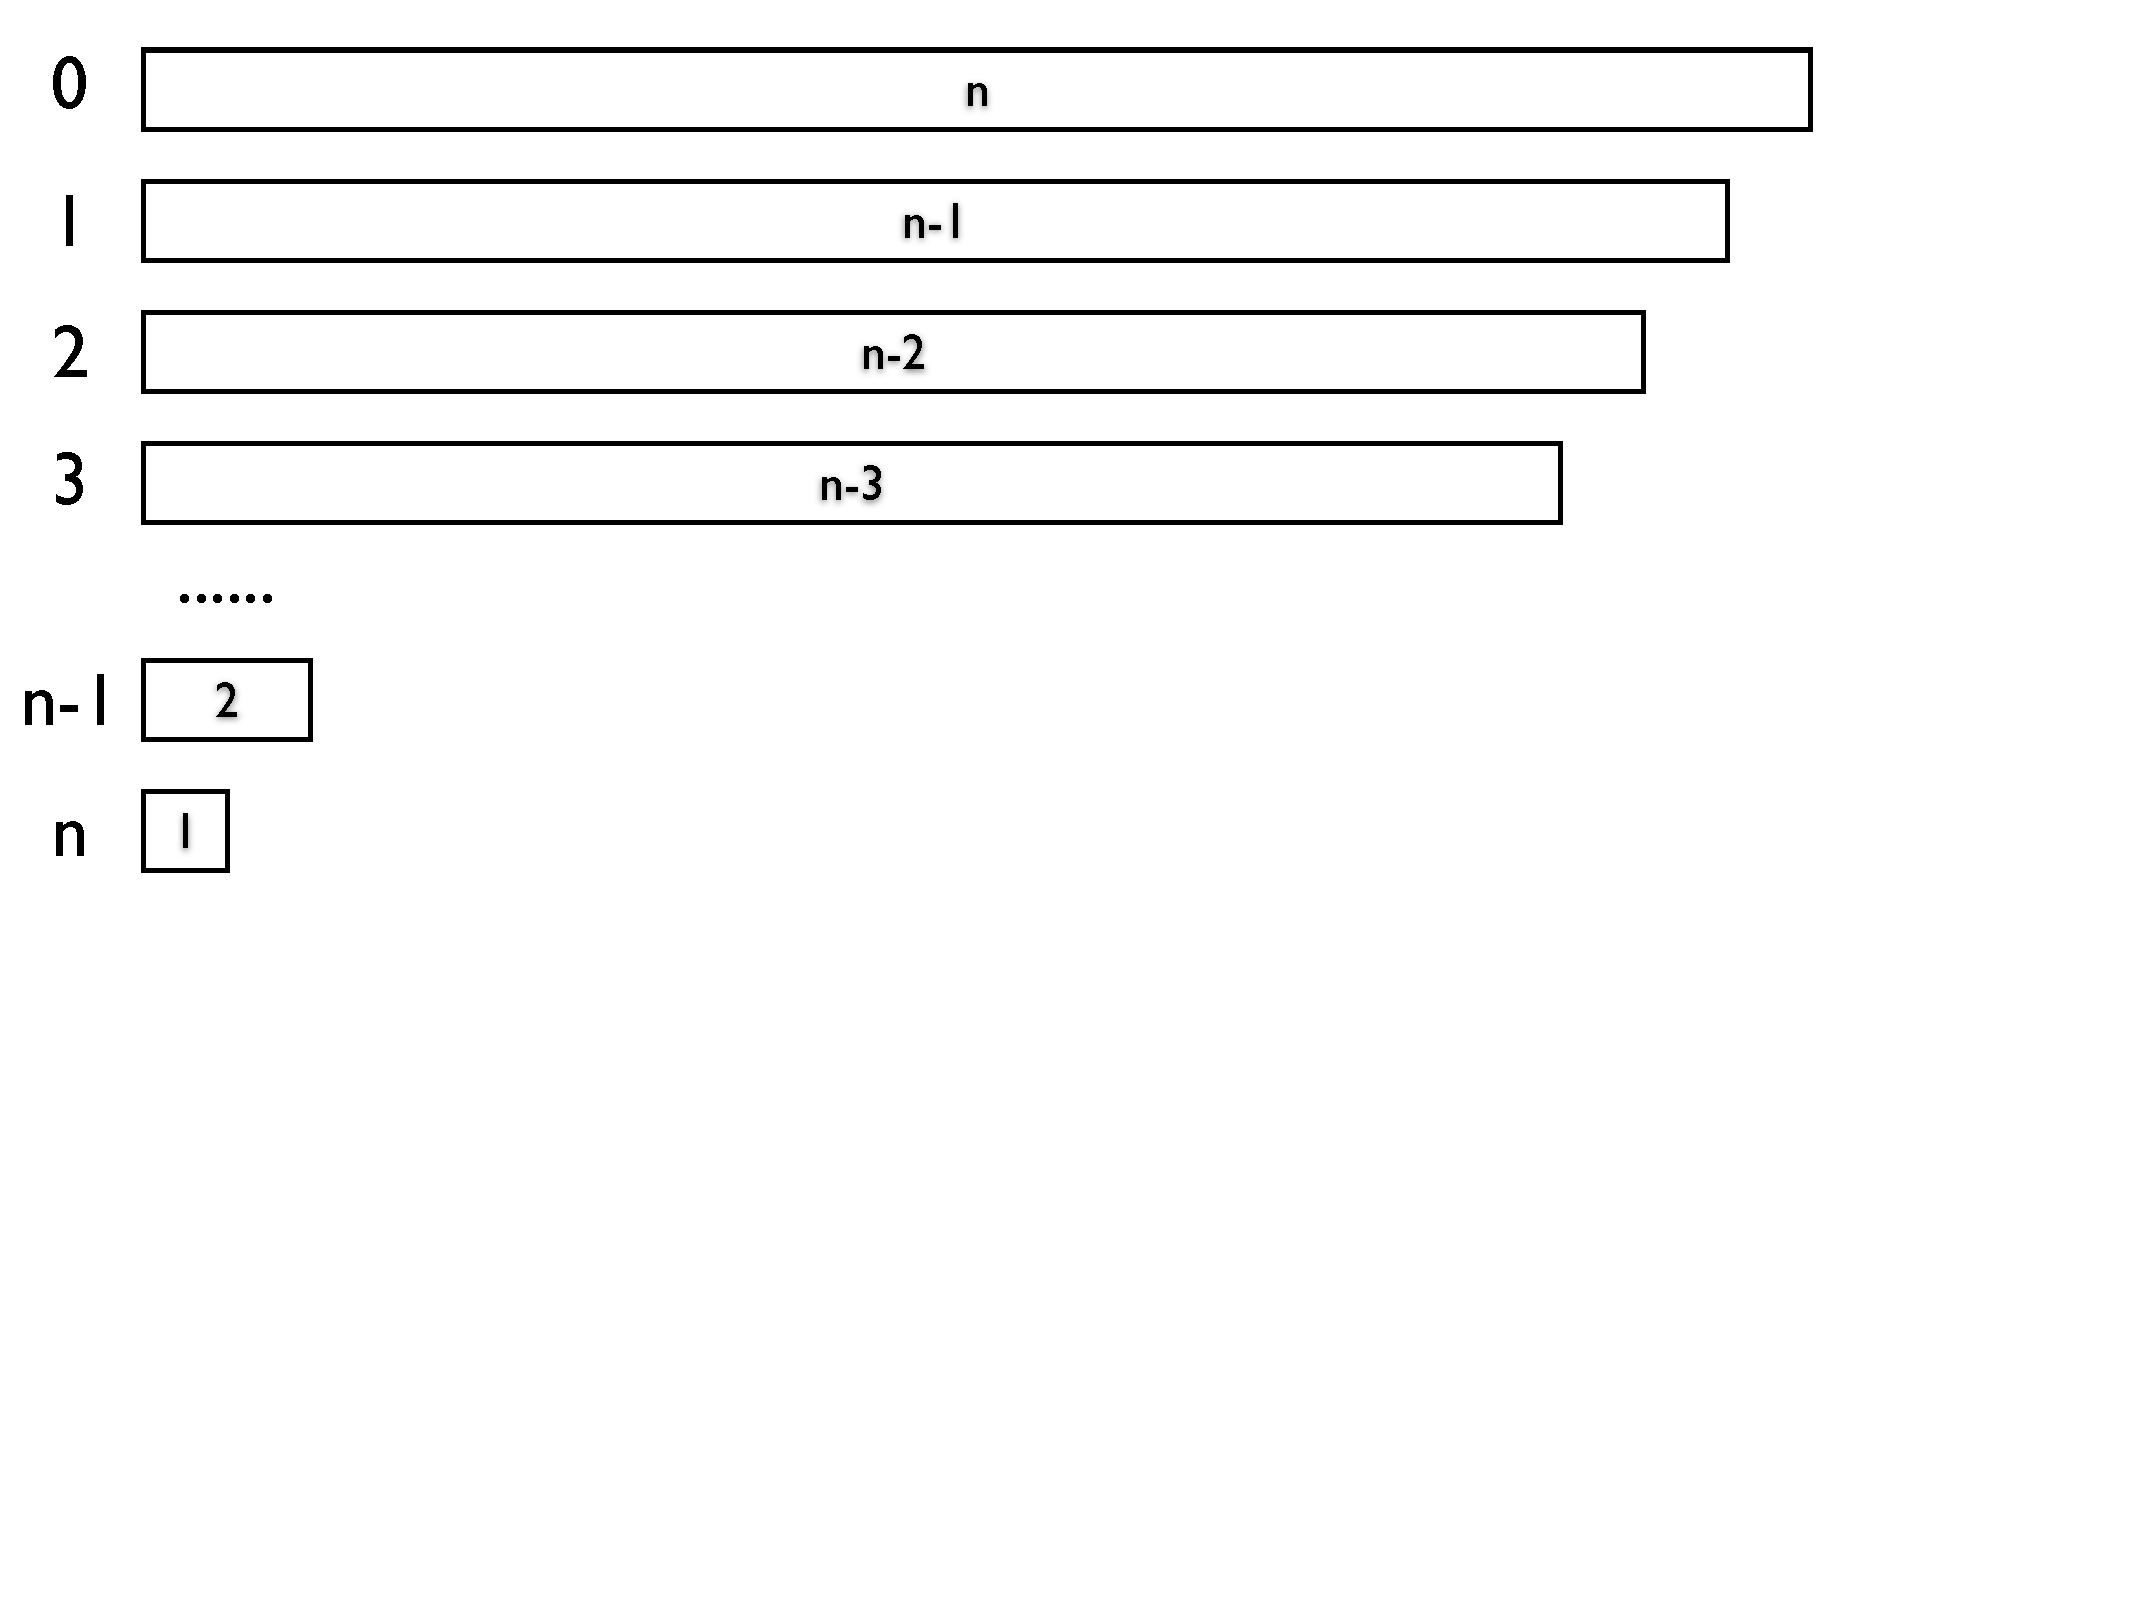
\includegraphics[width=.6\textwidth]{ennemenouno}
	\caption[]{Rappresentazione della ricorrenza lineare.}
\end{figure}

Possiamo rappresentare la funzione nel seguente modo:
\[
	T(n) = \sum_{i=1}^{n} i = \frac{n (n + 1)}{2} = \Theta(n^2)
\]

Effettuiamo un tentativo e proviamo a dimostrare che \fbox{\(T(n) = \Omicron(n)\)}

\textbf{Limite superiore}: Dobbiamo dimostrare che \(\exists c > 0, \exists m \geqslant 0 \,\colon T(n) \leqslant cn, \forall n \geqslant m\).
\begin{itemize}
	\item \textbf{caso base} lo saltiamo perché vedremmo subito che è sbagliato.
	\item \textbf{ipotesi induttiva} \(\forall k < n \,\colon T(k) \leqslant ck\).
	\item \textbf{passo induttivo} dimostriamo la disequazione per \(T(n)\):
	\[\begin{WithArrows}
	T(n) &= T(n-1) + n \Arrow{sost. ip. ind. con \(k = n-1\)}\\
	&= c(n-1) + n \Arrow{moltiplico}\\
	&= cn - c + n \Arrow{raccolgo \(n\)}\\
	&= (c+1)n - c \Arrow{rimuovo l'elemento negativo}\\
	&\leqslant (c+1)n \Arrow{obiettivo}\\
	&= (c+1)n \overset{?}{\leqslant} cn \Arrow{semplifico}\\
	&\Rightarrow c+1 \leqslant c
	\end{WithArrows}\]

	Possiamo notare che l'ultima disequazione risulta impossibile.
	Dunque quando proviamo a dimostrare qualcosa di sbagliato non riusciremo a dimostrarlo.
\end{itemize}

\subsection*{Difficoltà matematica}

\[
T(n) =
	\begin{cases}
	T(\floor{ \frac{n}{2} }) + T(\ceil{ \frac{n}{2} }) + 1 & n > 1 \\
	1 & n \leqslant 1
	\end{cases}
\]

\begin{note}
\`{E} possibile ottenere questa equazione di riccorrenza dall'algoritmo che calcola il minimo di un vettore non ordinato in maniera ricorsiva.
\end{note}

\begin{figure}[H]
	\centering
	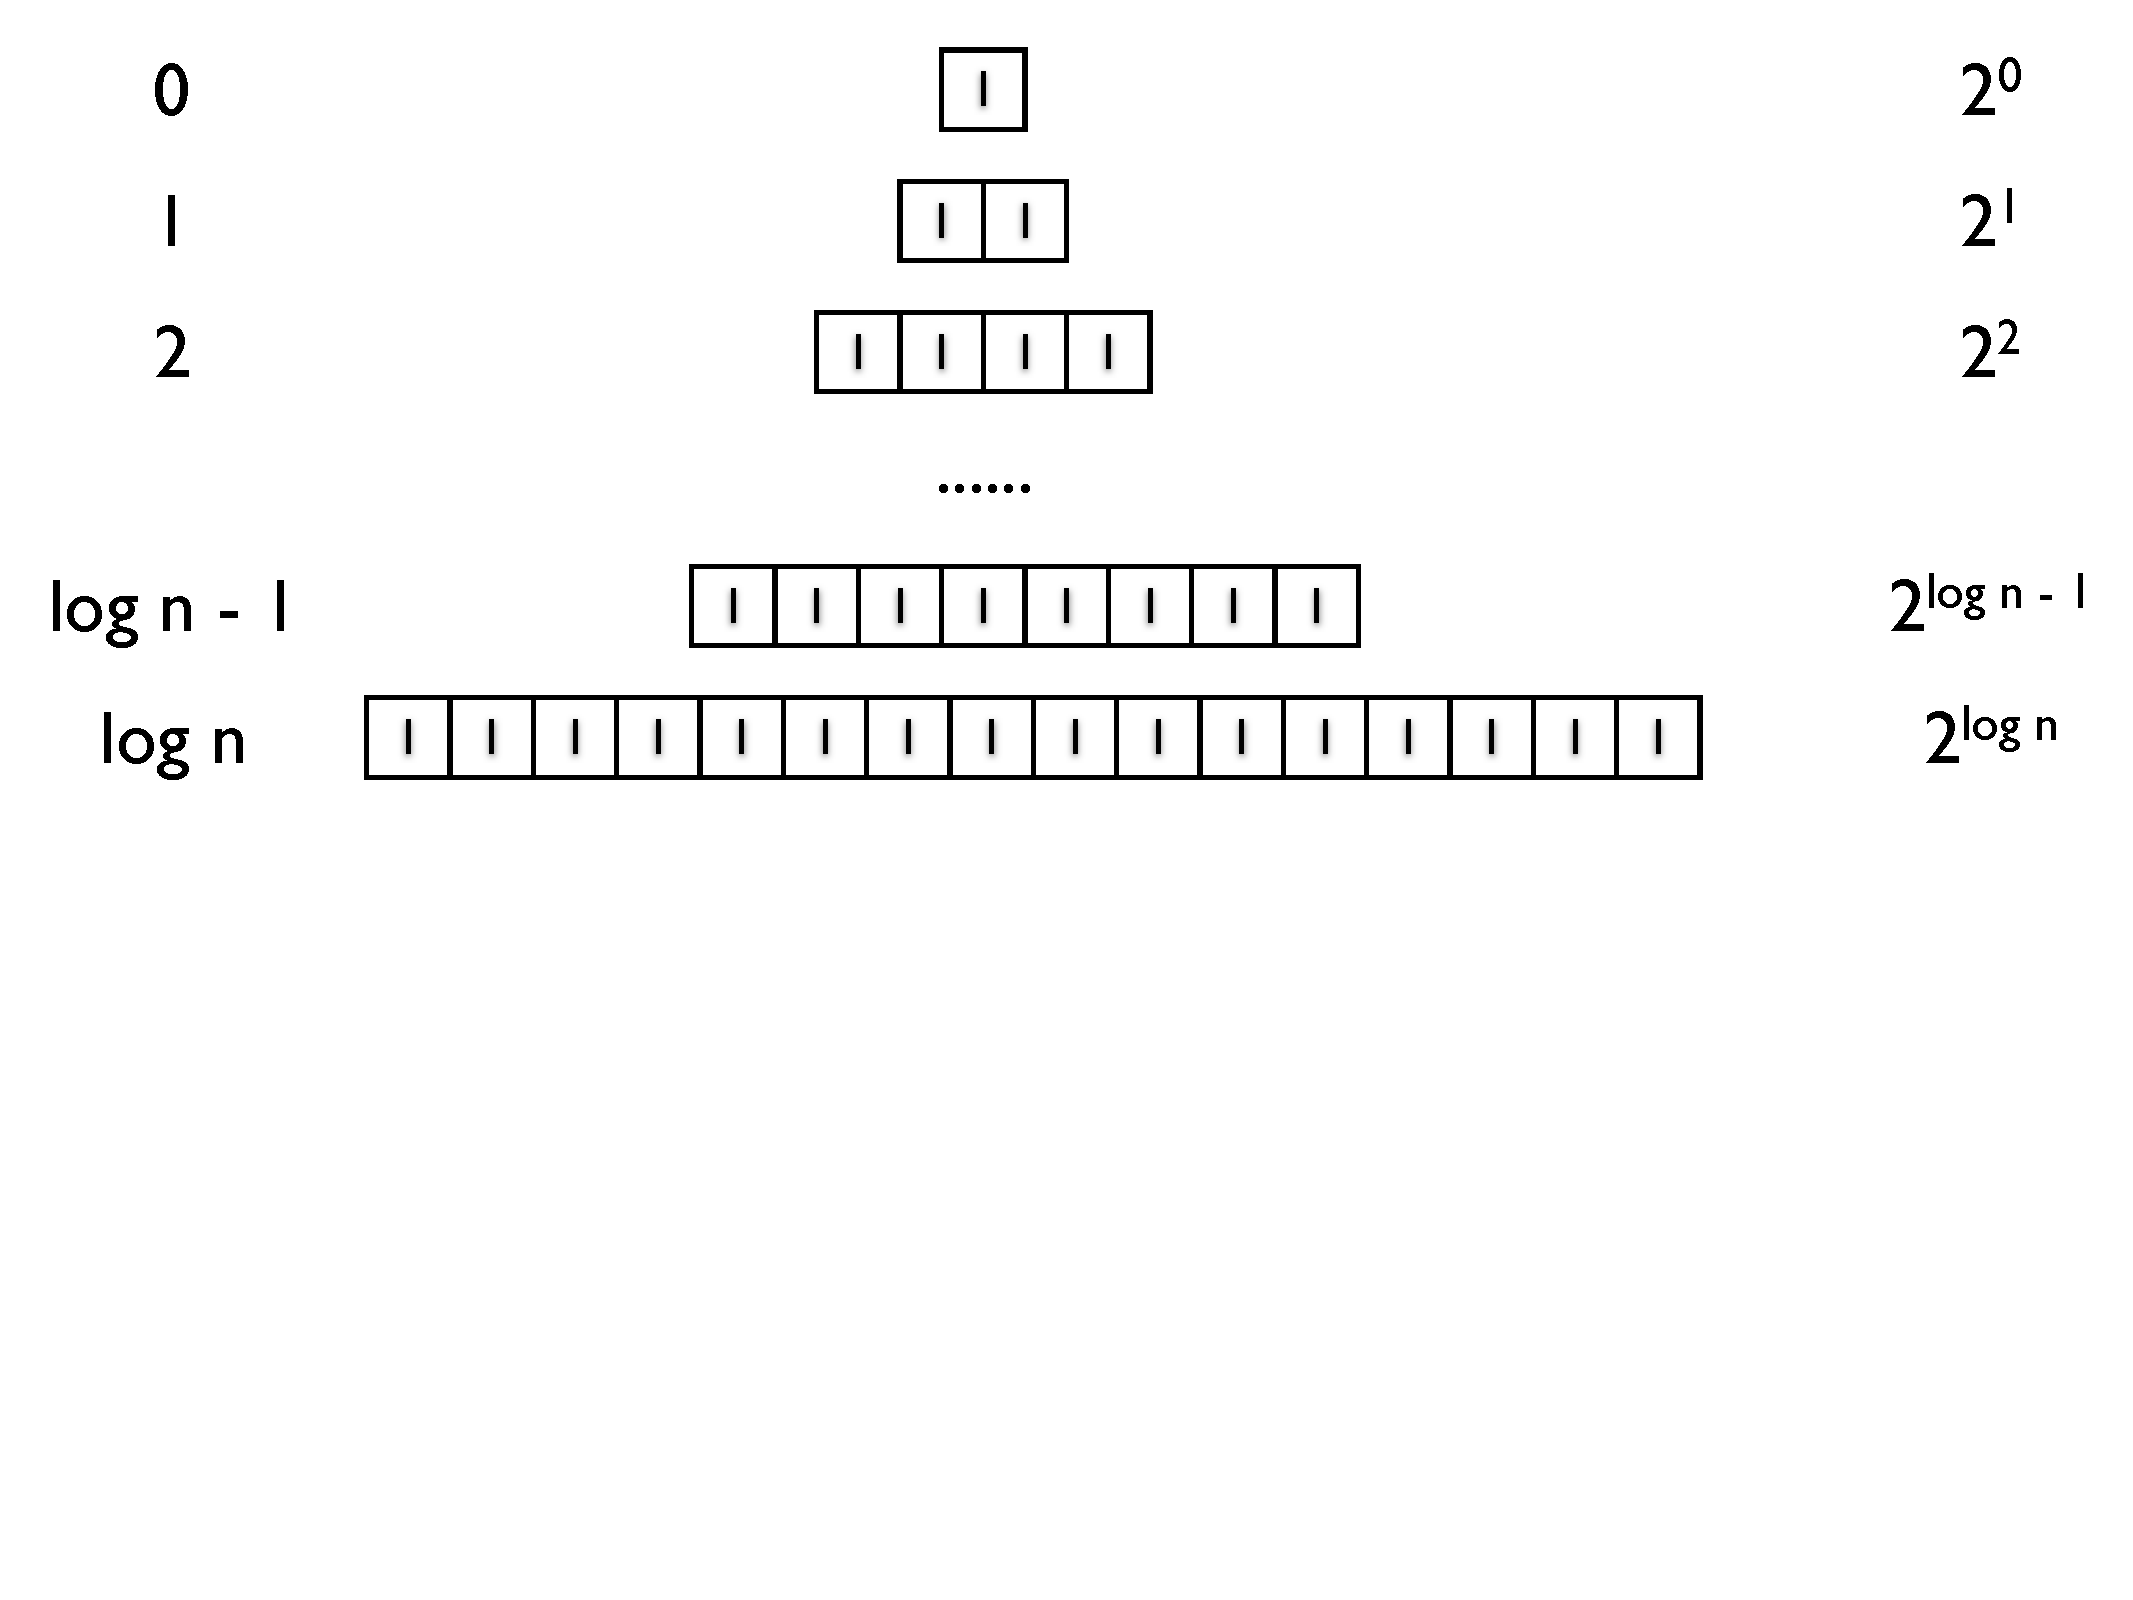
\includegraphics[width=.6\textwidth]{tree1}
	\caption[]{Rappresentazione della ricorsione.}
\end{figure}

\[
	T(n) = \sum_{i=0}^{\log n} 2^i = n + \frac{n}{2} + \frac{n}{4} + \cdots + 1 = \Omicron(n)
\]

Effettuiamo un tentativo per \fbox{\(T(n) = \Omicron(n)\)}

\begin{itemize}
	\item \textbf{ipotesi induttiva}: \(\forall k < n \,\colon T(k) \leqslant ck\).
	\item \textbf{passo induttivo}: dimostriamo la disequazione per \(T(n)\):
	\clearpage
	\[\begin{WithArrows}
	T(n) &= T(\floor{ \frac{n}{2} }) + T(\ceil{ \frac{n}{2} }) + 1 \Arrow{sost. ip. ind.}\\
		 &= c(\floor{ \frac{n}{2} }) + c(\ceil{ \frac{n}{2} }) + 1 \Arrow{semplifichiamo, \(\floor{ \frac{n}{2} } + \ceil{ \frac{n}{2} } = n\)}\\
		 &= cn + 1 \Arrow{obiettivo}\\
		 &= cn + 1 \overset{?}{\leqslant} cn \Arrow{semplifico}\\
		 &\Rightarrow 1 \leqslant 0
	\end{WithArrows}\]

	Anche in questo caso notiamo che l'ultima disequazione risulta impossibile, ma \mbox{-- a differenza del caso precendente --} non riusciamo a dimostrare il passo induttivo per un termine di ordine inferiore.
	Il tentativo risulta quindi errato.

	Proviamo quindi ad utilizzare un'ipotesi induttiva \emph{più stretta}.

	\item \textbf{ipotesi induttiva più stretta}: \(\exists c > 0, \exists m \geqslant 0 \,\colon T(n) \leqslant cn - b, \forall n \geqslant m\), \(b > 0\).

	Abbiamo introdotto una costante \(b > 0\) nella nostra tesi, questa modifica ci permetterà di dimostrare correttamente il passo induttivo.

	\item \textbf{ipotesi induttiva} \(\exists b > 0, \forall k < n \,\colon T(k) \leqslant ck - b\).

	\item \textbf{passo induttivo} dimostriamo la disequazione per \(T(n)\):
	\[\begin{WithArrows}
	T(n) &= T(\floor{ \frac{n}{2} }) + T(\ceil{ \frac{n}{2} }) + 1 \Arrow{sost. ip. ind.}\\
	&= c(\floor{ \frac{n}{2} }) - b + c(\ceil{ \frac{n}{2} }) - b + 1 \Arrow{semplifichiamo}\\
	&= cn -2b + 1 \Arrow{obiettivo}\\
	&= cn -2b + 1 \overset{?}{\leqslant} cn - b\Arrow[jump=2]{semplifico}\\
	&\Leftrightarrow -2b + 1 \leqslant -b\\
	&\Leftrightarrow b \geqslant 1
	\end{WithArrows}\]

	\item \textbf{caso base}
	\[T(1) = 1 \overset{?}{\leqslant} c \cdot 1 - b \Leftrightarrow c \geqslant b + 1\]
	Per concludere abbiamo provato che \(T(n) \leqslant cn - b \leqslant cn\) con diversi valori delle costanti \(c\) e \(b\), nel passo induttivo \(\forall b \geqslant 1, \forall c\), nel caso base \(\forall c \geqslant b+1\).
	Una coppia di valori di \(b\) e \(c\) che rispettano queste disequazioni sono \(b = 1\), \(c = 2\).

	Questo vale per \(n = 1\), e per tutti i valori di \(n\) successivi, quindi per \(m = 1\).

	Abbiamo quindi provato che \(T(n) = \Omicron(n)\).
\end{itemize}

Dimostriamo il limite inferiore facendo un tentativo per \fbox{\(T(n) = \Omega(n)\)}

Dobbiamo dimostrare che \(\exists d > 0, \exists m \geqslant 0 \,\colon T(n) \geqslant dn, \forall n \geqslant m\).

\begin{itemize}
	\item \textbf{passo induttivo}
	\[\begin{WithArrows}
	T(n) &= T(\floor{ \frac{n}{2} }) + T(\ceil{ \frac{n}{2} }) + 1 \Arrow{sost. ip. ind.}\\
	&\geqslant d(\floor{ \frac{n}{2} }) + d(\ceil{ \frac{n}{2} }) + 1 \Arrow{semplifichiamo}\\
	&= dn + 1 \Arrow{obiettivo}\\
	&= dn + 1 \overset{?}{\geqslant} dn
	\end{WithArrows}\]
	L'ultima disequazione risulta vera \(\forall d\).
	\item \textbf{caso base}
	\[T(n) = 1 \geqslant d \cdot 1 \iff d \leqslant 1\]

	Abbiamo quindi provato che \(T(n) = \Omega(n)\)
\end{itemize}

\subsection*{Problemi con i casi base}

\[
	T(n) =
	\begin{cases}
		2T(\floor{ \frac{n}{2} }) + n & n > 1 \\
		1 & n \leqslant 1
	\end{cases}
\]
Proviamo a visualizzarlo graficamente così:

\begin{figure}[H]
	\centering
	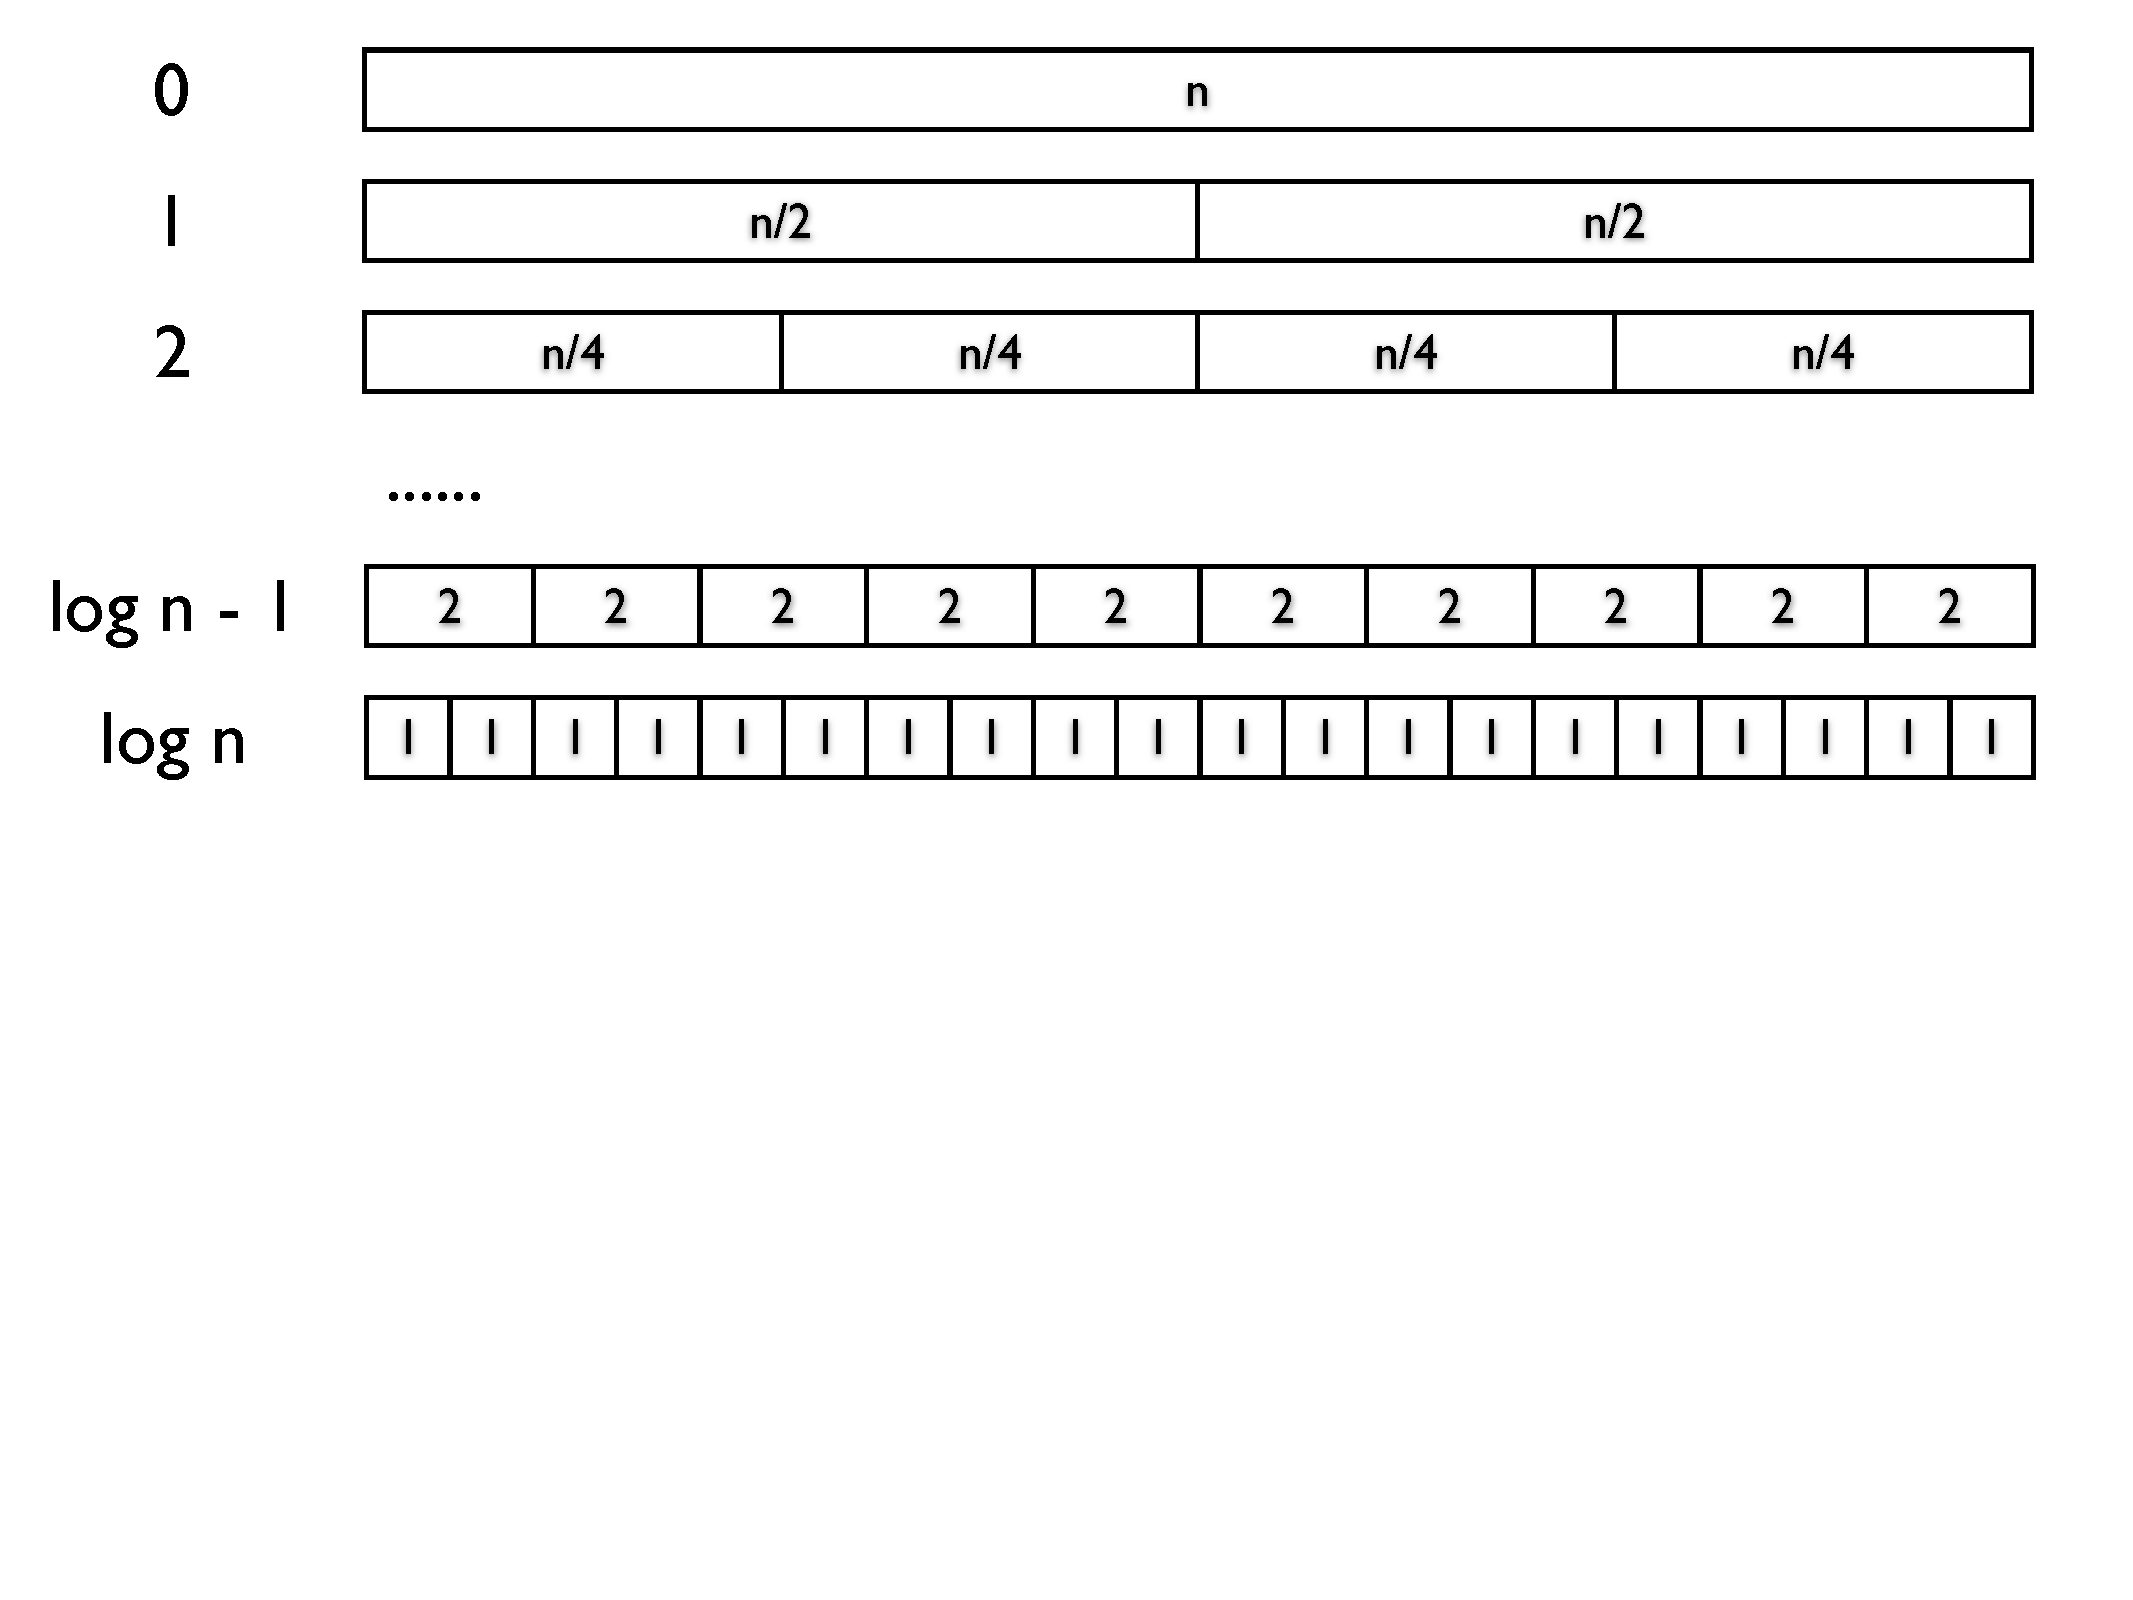
\includegraphics[width=.6\textwidth]{mergesort}
	\caption[]{Rappresentazione della ricorsione.}
\end{figure}

\begin{note}
\`{E} molto simile all'equazione dell'algoritmo \mergeSort che sappiamo avere una complessità di \(\Omicron(n \log n)\).
\end{note}

Effettuiamo un tentativo per \fbox{\(T(n) = \Omicron(n \log n)\)}

Dobbiamo dimostrare che \(\exists c > 0, \exists m \geqslant 0 \,\colon T(n) \leqslant cn \log n, \forall n \geqslant m\).

\begin{itemize}
	\item \textbf{Ipotesi induttiva}: \(\exists c > 0, \forall k < n \,\colon T(k) \leqslant ck \log k\)
	\item \textbf{Passo di induzione}: Dimostriamo la disequazione per \(T(n)\):
	\[\begin{WithArrows}
	T(n) &= 2T(\floor{ \frac{n}{2} }) + n \Arrow{sost. ip. ind. con \(k = \floor{\frac{n}{2}}\)}\\
		 &\leqslant 2c\floor{ \frac{n}{2} } \log \floor{ \frac{n}{2} } + n \Arrow{rimuovo l'intero inferiore}\\
		 &\leqslant \Ccancel{2}c \frac{n}{\Ccancel{2}} \log \frac{n}{2} + n \Arrow{semplifico}\\
		 &= cn \log \frac{n}{2} + n \Arrow{\(\log \frac{n}{2} = \log n - \log_2 2 = \log n - 1\)}\\
		 &= cn (\log n - 1) + n \Arrow{moltiplico}\\
		 &= cn \log n - cn + n \Arrow{obiettivo}\\
		 &\leqslant cn \log n - cn + n \overset{?}{\leqslant} cn \log n \Arrow[jump=2]{semplifico}\\
		 &\Leftrightarrow -cn + n \leqslant 0\\
		 &\Leftrightarrow c \geqslant 1
	\end{WithArrows}\]
	\item \textbf{caso base}: dimostriamo la disequazione per \(T(1)\)
	\[T(1) = 1 \overset{?}{\leqslant} 1 \cdot c \log 1 = 0 \Rightarrow 1 \nleq 0\]
	\`{E} falso, ma non è un problema, non a caso si chiama notazione asintotica: il valore di \(m\) lo possiamo scegliere noi.
	\item \textbf{caso base}: dimostriamo la disequazione per \(T(2)\), \(T(3)\)
	\begin{align*}
		T(2) &= 2T(\floor{\frac{2}{2}}) + 2 = 4 \leqslant 1 \cdot c \cdot 2 \log 2 \Leftrightarrow c \geqslant 2\\
		T(3) &= 2T(\floor{\frac{3}{2}}) + 3 = 5 \leqslant 1 \cdot c \cdot 3 \log 3 \Leftrightarrow c \geqslant \frac{5}{3 \log 3}\\
		T(4) &= 2T(\floor{\frac{4}{2}}) + 4 = 2T(\floor{2}) + 4
	\end{align*}
	Non è necessario provare la terza disequazione, in quanto viene espressa in base ai casi base diversi da \(T(1)\) che sono già stati dimostrati e quindi possono costituire la base per la nostra induzione.
\end{itemize}

Riassumendo:
\begin{itemize}
	\item[] Abbiamo provato che \(T(n) \leqslant cn \log n\)
	\begin{itemize}[label=\textbullet]
		\item nel passo induttivo: \(\forall c \geqslant 1\)
		\item nel caso base: \(\forall c \geqslant 2, c \geqslant \frac{5}{3\log 3}\)
	\end{itemize}
	Visto che sono tutte disequazioni con il segno \(\geqslant\), è sufficiente utilizzare \(c \geqslant \maxFunction\left\{ 1,2,\frac{5}{3 \log 3} \right\}\)

	Questo vale per \(n=2\), \(n=3\), e per tutti i valori di \(n\) successivi, quindi \(m = 2\).
\end{itemize}

\subsection*{Ultimo esercizio}

\[
	T(n) =
	\begin{dcases}
	9 T( \floor{\nicefrac{n}{3} }) + n & n > 1 \\
	1 & n \leqslant 1 \\
	\end{dcases}
\]

Effettuiamo un tentantivo \fbox{\(T(n) = \Omicron(n^2)\)}

Dobbiamo dimostrare che \(\exists c > 0, \exists m \geqslant 0 \,\colon T(n) \leqslant cn^2, \forall n \geqslant m\)
\begin{itemize}
	\item \textbf{ipotesi induttiva}: \(\exists c > 0 \,\colon T(k) \leqslant ck^2, \forall k < n\)
	\item \textbf{passo induttivo} dimostriamo la disequazione per \(T(n)\):
	\[\begin{WithArrows}
	T(n) &= 9T\left( \floor{\frac{n}{3}} \right) + n \Arrow{sost. ip. ind. con \(k = \floor{\frac{n}{3}}\)}\\
		 &\leqslant 9 c{\left( \floor{\frac{n}{3}} \right)}^{2} + n \Arrow{rimuovo l'intero inferiore}\\
		 &\leqslant 9 c \left( \frac{n^2}{9} \right) + n \Arrow{semplifico il \(9\)}\\
		 &= cn^2 + n \Arrow{obiettivo}\\
		 &= cn^2 + n \leqslant cn^2
	\end{WithArrows}\]
	L'ultima disequazione risulta falsa per un termine di ordine inferiore: proviamo quindi a modificare l'ipotesi induttiva e a ripetere il passo induttivo.
	\item \textbf{ipotesi induttiva più stretta} \(\exists c > 0 \,\colon T(k) \leqslant c(k^2 - k), \forall k < n\)
	\item \textbf{passo induttivo} dimostriamo la disequazione per \(T(n)\):
	\[\begin{WithArrows}
	T(n) &= 9T\left( \floor{\frac{n}{3}} \right) + n \Arrow{sost. ip. ind. con \(k = \floor{\frac{n}{3}}\)}\\
		 &\leqslant 9c \left( {\floor{\frac{n}{3}}}^{2} - \floor{\frac{n}{3}} \right) + n \Arrow{rimuovo l'intero inferiore}\\
		 &\leqslant 9c \left( {\left(\frac{n}{3}\right)}^{2} - \frac{n}{3} \right) + n \Arrow{svolgo la potenza}\\
		 &\leqslant 9c \left( \frac{n^2}{9} - \frac{n}{3} \right) + n \Arrow{moltiplico}\\
		 &\leqslant cn^2 - 3cn + n \Arrow{obiettivo}\\
		 &\leqslant cn^2 - 3cn + n \overset{?}{\leqslant} cn^2 - cn \Arrow[jump=2]{semplifico}\\
		 &\Leftrightarrow 2 cn \geqslant cn\\
		 &\Leftrightarrow c \geqslant \frac{1}{2}
	\end{WithArrows}\]
	\item \textbf{caso base}
	\begin{align*}
		T(1) &= 1 \leqslant c(1^2 - 1) = 0, falso\\
		T(2) &= 9T(0) + 2 = 11 \leqslant c(2^2 - 2) \Leftrightarrow c \geqslant \nicefrac{11}{2}\\
		T(3) &= 9T(1) + 3 = 12 \leqslant c(3^2 - 3) \Leftrightarrow c \geqslant \nicefrac{12}{6}\\
		T(4) &= 9T(1) + 4 = 13 \leqslant c(4^2 - 4) \Leftrightarrow c \geqslant \nicefrac{13}{12}\\
		T(5) &= 9T(1) + 5 = 14 \leqslant c(5^2 - 5) \Leftrightarrow c \geqslant \nicefrac{14}{20}\\
		T(6) &= 9T(2) + 6
	\end{align*}
	Non è necessario andare oltre poiché T(6) dipende da T(2) che è già stato dimostrato.

	Riassumendo i parametri scelti sono:
	\begin{itemize}[label=\textbullet]
		\item \(c \geqslant \maxFunction \left\{ \frac{1}{2},\frac{11}{2},\frac{12}{6},\frac{13}{12},\frac{14}{20} \right\}\)
		\item \(m = 1\)
	\end{itemize}
	Nota che l'esempio combina le due difficoltà insieme, ma è stato creato artificiosamente: infatti se avessimo scelto come ipotesi più stretta \(T(n) \leqslant cn^2 - bn\), il problema sui casi base non si sarebbe posto.

	Abbiamo quindi dimostrato che \(T(n) \leqslant c(n^2 - n) \leqslant cn^2, \forall n \geqslant 1, \forall c \geqslant \frac{14}{20}\), ossia che \(T(n) = \Omicron(n)\)
\end{itemize}

\subsection*{Riassumendo}

Il metodo di sostituzione è composto da tre parti:
\begin{enumerate}
	\item si \emph{indovina} una possibile soluzione e si formula un'ipotesi induttiva;
	\item si \emph{sostituisce} nella ricorrenza le espressioni \(T(\,\cdot\,)\), utilizzando l'ipotesi induttiva;
	\item si \emph{dimostra} che la soluzione è valida anche per il caso base.
\end{enumerate}

Bisogna fare attenzione:
\begin{itemize}
	\item ad ipotizzare soluzioni troppo \enquote{strette};
	\item ad alcuni casi particolari che richiedono astuzie matematiche;
	\item ai casi base in cui compare il logaritmo in quanto potrebbe complicare le cose.
\end{itemize}

\clearpage
\section{Metodo dell'esperto (o delle ricorrenze comuni)}

Esiste un'ampia classe di ricorrenze che possono essere risolte facilmente facendo ricorso ad alcuni teoremi, ognuno dei quali si occupa di una classe particolare di equazioni di ricorrenza.

\begin{theorem}[ricorrenze lineari con partizione bilanciata]
Siano \(a\) e \(b\) costanti intere tale che \(a \geqslant 1\) e \(b \geqslant 2\), e \(c\), \(\beta\) costanti reali tali che \(c > 0\) e \(\beta \geqslant 0\).
Sia \(T(n)\) data dalla relazione di ricorrenza:
\[
	T(n) =
	\begin{dcases}\textstyle
		a\T{\frac{n}{b}} + cn^{\beta} & n > 1 \\
		d & n \leqslant 1 \\
	\end{dcases}
\]
Posto \(\alpha = \frac{\log a}{\log b} = \log_{b} a\), allora:
\[
	T(n) =
	\begin{dcases}
		\Theta(n^{\alpha}) & \alpha > \beta \\
		\Theta(n^{\alpha}\log n) & \alpha = \beta \\
		\Theta(n^{\beta}) & \alpha < \beta \\
	\end{dcases}
\]
\end{theorem}

\paragraph{Commento}
Affrontiamo le equazioni di ricorrenza in cui la dimensione viene divisa in \(b\) parti, dove \(b\) dev'essere almeno pari a 2; l'algoritmo ricorsivo dev'essere richiamato \(a\) volte, dove \(a\) è almeno 1.
Nella versione estesa, che vedremo fra poco, vedremo che i parametri \(a\) e \(b\) verranno \enquote{rilassati}.

Prendiamo ad esempio il primo esercizio \(T(n) = 4T(\frac{n}{2})\) e vediamo che si può risolvere semplicemente calcolando \(\alpha = \log_b a = \log_2 4 = 2 > \beta = 1\), possiamo quindi concludere che \(T(n) = \Theta(n^{\alpha}) = \Theta(n^2)\).

\begin{proof}[Dimostrazione del teorema delle ricorrenze lineari con partizione bilanciata]
Assumiamo che \(n\) sia una potenza intera di \(b\), ossia che \(n = b^k\), \(k = \log_b n\) poiché ci permetterà di semplificare i calcoli successivi ed è ininfluente sul risultato.
Ad esempio supponiamo che l'input abbia dimensione \(b^k + 1\) (\(2^8 + 1 = 257\) bit), se estendiamo l'input fino ad una dimensione \(b^{k+1}\) (\(2^8+1 = 512\) bit, facendo del \foreign{padding}, l'input sarebbe stato esteso al massimo di un fattore costante \(b\) (\(2\) nel nostro caso), il che è ininfluente al fine della complessità computazionale.

Calcoliamo l'albero delle ricorrenze per la seguente equazione di ricorrenza:
\[
	T(n) =
	\begin{dcases}\textstyle
		a\T{\frac{n}{b}} + cn^{\beta} & n > 1 \\
		d & n \leqslant 1 \\
	\end{dcases}
\]

\clearpage
\begin{center}
	\begin{tabular}{@{} *{5}{c} @{}}
		\toprule
			livello & dim. & costo chiam. & no. chiamate & costo livello \\
		\midrule
			\(0\) & \(b^k\) & \(c\,b^{k\beta}\) & \(1\) & \(cb^{k\beta}\) \\
		\addlinespace
			\(1\) & \(b^{k-1}\) & \(c\,b^{(k-1)\beta}\) & \(a\)  & \(a \cdot c\, b^{(k-1)\beta}\)\\
		\addlinespace
			\(2\) & \(b^{k-2}\) & \(c\,b^{(k-2)\beta}\) & \(a^2\) & \(a^2 \cdot c\, b^{(k-2)\beta}\)\\
		\addlinespace
			\(\vdots\) & \(\vdots\) & \(\vdots\) & \(\vdots\) & \(\vdots\) \\
		\addlinespace
			\(i\) & \(b^{k-i}\) & \(c\,b^{(k-i)\beta}\) & \(a^i\) & \(a^i \cdot c\, b^{(k-i)\beta}\)\\
		\addlinespace
			\(\vdots\) & \(\vdots\) & \(\vdots\) & \(\vdots\) & \(\vdots\) \\
		\addlinespace
			\(k-1\) & \(b\) & \(c b^{(k-(k-1))\beta} = c\,b^{\beta}\) & \(a^{k-1}\) & \(a^{k-1} \cdot c\, b^{\beta}\) \\
		\addlinespace
			\(k\) & \(1\) & \(d\) & \(a^k\) & \(a^k \cdot d\) \\
		\bottomrule
	\end{tabular}
\end{center}

Sommando i costi totali del \(k\)-esimo livello e dei livelli fino al \(k-1\), si ottiene:
\[\begin{WithArrows}[displaystyle]
T(n) &= da^k + \sum_{i=0}^{k-1} a^i \cdot c b^{(k-i)\beta} \Arrow{moltiplico}\\
	 &= da^k + \sum_{i=0}^{k-1} a^i \cdot c b^{k\beta} \cdot b^{-i\beta} \Arrow{porto fuori i termini\\non dipendenti da \(i\)}\\
	 &= da^k + cb^{k\beta} \sum_{i=0}^{k-1} \frac{a^i}{b^{i\beta}} \Arrow{raccolgo \(i\)}\\
	 &= da^k + cb^{k\beta} \sum_{i=0}^{k-1} \left( \frac{a}{b^{\beta}} \right)^{i}
\end{WithArrows}\]
A questo punto ho una formula chiusa ma non ancora nella sua forma definitiva.

\
Facciamo alcune osservazioni.
\begin{itemize}[label=\textbullet]
	\item \(a^k = a^{\log_b n} = a^{\frac{\log n}{\log b}} = 2^{\log_2 a \frac{\log n}{\log b}} = 2^{\log_2 n \frac{\log a}{\log b}} = n^{\frac{\log a}{\log b}} = n^{\alpha}\)

	\item \(\alpha = \frac{\log a}{\log b} \Leftrightarrow \alpha\log b = \log a \Leftrightarrow \log b^{\alpha} = \log a \Leftrightarrow a = b^{\alpha}\)

	\item poniamo \(q = \frac{a}{b^{\beta}} = \frac{b^{\alpha}}{b^{\beta}} = b^{\alpha-\beta}\)
\end{itemize}
Grazie alle osservazioni appena fatto possiamo sostituire i parametri nell'equazione finale:
\[\begin{WithArrows}[displaystyle]
T(n) &= da^k + cb^{k\beta} \sum_{i=0}^{k-1} \left( \frac{a}{b^{\beta}} \right)^{i} \Arrow{sostituisco: \(\alpha^k \rightarrow n^{\alpha}\)\\sostituisco: \(a \rightarrow b^{\alpha}\), \(q = \frac{b^{\alpha}}{b^{\beta}}\)}\\
	 &= dn^{\alpha} + cb^{k\beta} \sum_{i=0}^{k-1} q^{i}
\end{WithArrows}\]
Da qui si aprono tre possibilità, ossia che
\begin{enumerate*}
	\item \(\alpha > \beta\)
	\item \(\alpha = \beta\)
	\item \(\alpha < \beta\)
\end{enumerate*}
Studiamole una per una.

\begin{enumerate}
	\item Caso \fbox{\(\alpha > \beta\)}, ne segue che \(q = b^{\alpha - \beta} > 1\)
	\[\begin{WithArrows}[displaystyle]
	T(n) &= dn^{\alpha} + cb^{k\beta} \sum_{i=0}^{k-1} q^{i} \Arrow{serie geometrica finita}\\
		 &= n^{\alpha}d + cb^{k\beta} \left[ \frac{q^k - 1}{q-1} \right] \Arrow{introduco la disequazione}\\
		 &\leqslant n^{\alpha}d + cb^{k\beta} \frac{q^k}{q-1} \Arrow{sostituisco: \(q = \frac{a}{b^{\beta}} \Rightarrow q^k = \frac{a^k}{b^{k\beta}}\)}\\
		 &= n^{\alpha}d + \frac{cb^{k\beta}a^k}{b^{k\beta}} \frac{1}{q-1} \Arrow{semplifico: \(b^{k\beta}\)}\\
		 &= n^{\alpha}d + \frac{ca^k}{q-1} \Arrow{sostituisco: \(a^k = n^{\alpha}\)}\\
		 &= n^{\alpha}d + \frac{cn^{\alpha}}{q-1} \Arrow{raccolgo per \(n^{\alpha}\)}\\
		 &= n^{\alpha} \left[ d + \frac{c}{q-1} \right]
	\end{WithArrows}\]
	Visto che \(d\), \(c\) e \(q\) sono tutti termini positivi e costanti possiamo concludere che \(n^{\alpha}\) limita superiormente l'espressione e che quindi \(T(n) = \Omicron(n^{\alpha})\).
	Infine per via della componente non ricorsiva \(dn^{\alpha}\), \(T(n)\) è anche \(\Omega(n^{\alpha})\), possiamo concludere che \(T(n) = \Theta(n^{\alpha})\).

	\item Caso \fbox{\(\alpha = \beta\)}, ne segue che \(q = b^{\alpha - \beta} = 1\)
	\[\begin{WithArrows}[displaystyle]
	T(n) &= dn^{\alpha} + cb^{k\beta} \sum_{i=0}^{k-1} q^{i} \Arrow{\(q^i = 1^i = 1\)\\\(1+2+\cdots+k-1 = k\)}\\
		 &= n^{\alpha}d + cn^{\beta}k \Arrow{sostituisco: \(\beta = \alpha\)}\\
		 &= n^{\alpha}d + cn^{\alpha}k \Arrow{raccolgo per \(n^{\alpha}\)}\\
		 &= n^{\alpha}(d + ck) \Arrow{sostituisco: \(k = \log_b n\)}\\
		 &= n^{\alpha}(d + c\textstyle\frac{\log n}{\log b})
	\end{WithArrows}\]
	Visto che \(d\), \(c\) e \(\log b\) sono tutti termini positivi e costanti e che non abbiamo introdotto disequazioni, possiamo affermare che \(T(n) = \Theta(n^{\alpha}\log n)\).

	\item Caso \fbox{\(\alpha < \beta\)}, ne segue che \(q = b^{\alpha - \beta} < 1\)
	\[\begin{WithArrows}[displaystyle]
	T(n) &= dn^{\alpha} + cb^k \sum_{i=0}^{k-1} q^i \Arrow{serie geometrica finita}\\
		 &= dn^{\alpha} + cb^k \left[ \frac{q^k - 1}{q-1} \right] \Arrow{inversione, \(1-q > 0\)}\\
		 &= dn^{\alpha} + cb^k \left[ \frac{1 - q^k}{1-q} \right] \Arrow{introduco\\la disequazione}\\
		 &\leqslant dn^{\alpha} + cb^k \left[ \frac{1}{1-q} \right] \Arrow{sostituisco: \(b^k = n\)}\\
		 &= n^{\alpha}d + \frac{cn^{\beta}}{1-q}
	\end{WithArrows}\]
	\(n^{\alpha} < n^{\beta}\) quindi considero il polinomio di grado maggiore, di conseguenza \(T(n)\) è \(\Omicron(n^{\beta})\).
	Poiché \(T(n) = \Omega(n^{\beta})\) per via del termine non ricorsivo, possiamo affermare che \(T(n) = \Theta(n^{\beta})\).
\end{enumerate}
Fine dimostrazione.
\end{proof}

\begin{theorem*}[ricorrenze lineari con partizione bilanciata estesa]
Sia \(a \geqslant 1\), \(b > 1\), \(f(n)\) asintoticamente positiva, e sia
\[
	T(n) =
	\begin{dcases}\textstyle
		a\T{\frac{n}{b}} + f(n) & n > 1 \\
		d & n \leqslant 1 \\
	\end{dcases}
\]
Sono dati tre casi:
\begin{enumerate}
	\item \(\exists \varepsilon > 0 \colon f(n) = \Omicron(n^{\alpha-\varepsilon})\) allora \(T(n) = \Theta(n^{\alpha})\);
	\item \(f(n) = \Theta(n^\alpha)\) allora \(T(n) = \Theta(f(n)\log n)\);
	\item \(\exists \varepsilon > 0 \,\colon f(n) = \Omicron(n^{\alpha + \varepsilon}) \land\\\exists c \,\colon 0 < c < 1, \exists m > 0 \,\colon\\a f(\frac{n}{b}) \leqslant c f(n), \forall n \geqslant m\) allora \(T(n) = \Theta(f(n))\).
\end{enumerate}
\end{theorem*}

Non vedremo la dimostrazione poiché è troppo complessa.

\paragraph{Commento}
Il teorema precendente funzionava con \(n^{\beta}\), aveva una serie di condizioni semplificative, ora non ci sono più.
Nel secondo caso se \(f(n) = n^{\beta}\) ritorniamo esattamente al secondo caso del teorema precendente, ma qui possiamo prendere in considerazione funzioni più complesse.

\subsection*{Esercizi}

Le soluzioni sono indicate fra parentesi.
\begin{itemize}
	\item \(T(n) = 9T(\frac{n}{3}) + n\) \hfill[\(\Omicron(n^{2-\varepsilon})\), con \(\varepsilon < 1\)]
	\item \(T(n) = T(\frac{2}{3} n) + 1\)  \hfill[\(\Theta(n^0)\)]
	\item \(T(n) = 3T(\frac{n}{4}) + n\log n\) \hfill[\(c = \nicefrac{3}{4}\), \(m = 1\)]
	\item \(T(n) = 2T(\frac{n}{2}) + n\log n\) \hfill[nessun caso applicabile]
\end{itemize}

\begin{theorem*}[ricorrenze lineari di ordine costante]
Siano \(\{a_1, a_2, \dots, a_n\}\) costanti intere non negative, con \(h\) costante positiva, \(c\) e \(\beta\) costanti reali tali che \(c > 0\) e \(\beta \geqslant 0\), e sia \(T(n)\) definita dalla relazione di ricorrenza:
\[
	T(n) =
	\begin{dcases}
		\sum_{1 \leqslant i \leqslant h} a_i \T{n-1} + cn^{\beta} & n > m \\
		\Theta(1) & n \leqslant m \leqslant h \\
	\end{dcases}
\]
Posto \(a = \sum_{1 \leqslant i \leqslant h} a_i\), allora:
\begin{enumerate}
	\item \(T(n)\) è \(\Theta(n^{\beta+1})\), se \(a = 1\);
	\item \(T(n)\) è \(\Theta(a^n n^{\beta})\), se \(a \geqslant 2\).
\end{enumerate}
\end{theorem*}

\paragraph{Commento}
Questo teorema tratta ricorrenze lineari \emph{di ordine costante} perché tutte le volte rimuoviamo dalla dimensione di input \(n\) una quantità costante.

\subsection*{Esercizi}

Le soluzioni sono indicate fra parentesi.
\begin{itemize}[label=\textbullet]
	\item \(T(n) = T(n-10) + n^2\) \hfill[costo polinomiale]
	\item \(T(n) = T(n-2) - T(n-1) + 1\) \hfill[costo esponenziale]
\end{itemize}

\ifsubfile
\end{document}
\fi

	%&../settings/preamble.main

\ifsubfile
\usepackage[newfloat, cachedir=_minted-cache, outputdir=../build]{minted}
\usepackage{../libraries/set-minted}

\pagestyle{plain}
\setcounter{chapter}{2}

% arara: pdflatex: { options: ["--output-directory=../build"], shell: yes, draft: yes, synctex: no }
% arara: pdflatex: { options: ["--output-directory=../build"], shell: yes, synctex: no }
\begin{document}
\fi
\section{Algoritmo della somma massimale di un sottovettore}

Date le nostre nuove conoscenze possiamo calcolare con precisione la complessità delle varie versioni degli algoritmi proposti per la soluzione al problema della somma massimale di un sottovettore.

\subsubsection*{Complessità della prima versione}

\begin{code}
\begin{minted}{cpp}
int maxsum1(int[] A, int n) {
	int maxSoFar = 0;
	for (int i = 0; i < n; i++) {
		for (int j = i; j < n; j++) {
			int sum = 0;
			for (int k = i; k <= j; k++) {
				sum = sum + A[k];
			}
			maxSoFar = max(maxSoFar, sum);
		}
	}
	return maxSoFar;
}
\end{minted}
% \captionof{listing}{Versione 1}
% \label{code:c-code}
\end{code}

La complessità dell'algoritmo può essere approssimata come segue (contando il numero di esecuzioni della riga più interna):
\[\begin{WithArrows}[displaystyle]
T(n) = \sum_{i=0}^{n-1} \sum_{j=i}^{n-1} (j - i + 1)
\end{WithArrows}\]

Vogliamo provare che \(T(n) = \Omicron(n^3)\).
\begin{proof}
\textbf{limite superiore}:
\(\exists c_2 > 0, \exists m \geqslant 0 : T(n) \leqslant c_2 n^3\), \(\forall n \geqslant m\).
\[\begin{WithArrows}[displaystyle]
T(n) &= \sum_{i=0}^{n-1} \sum_{j=i}^{n-1} (j - i + 1) \Arrow{spiegazione}\\
	 &\leqslant \sum_{i=0}^{n-1} \sum_{j=i}^{n-1} n \Arrow{spiegazione}\\
	 &\leqslant \sum_{i=0}^{n-1} \sum_{j=0}^{n-1} n \Arrow{spiegazione}\\
	 &=\sum_{i=0}^{n-1} n^2 \Arrow{spiegazione}\\
	 &= n^3 \leqslant c_2 n^3
\end{WithArrows}\]
Questa disequazione è vera per \(n \geqslant m = 0\) and \(c_2 \geqslant 1\).
\end{proof}

Vogliamo provare che \(T(n) = \Omega(n^3)\).
\begin{proof}
\textbf{limite inferiore}:
\(\exists c_1 > 0, \exists m \geqslant 0 : T(n) \leqslant c_1 n^3\), \(\forall n \geqslant m\).
\[\begin{WithArrows}[displaystyle]
T(n) &= \sum_{i=0}^{n-1} \sum_{j=i}^{n-1} (j - i + 1) \\
	 &\geqslant \sum_{i=0}^{\nicefrac{n}{2}} \sum_{j=i}^{n+\nicefrac{n}{2}-1} (j - i + 1) \Arrow{spiegazione}\\
	 &= \sum_{i=0}^{\nicefrac{n}{2}} \sum_{j=i}^{n+\nicefrac{n}{2}-1} \nicefrac{n}{2} \Arrow{spiegazione}\\
	 &= \sum_{i=0}^{\nicefrac{n}{2}} \nicefrac{n^2}{4} \geqslant \nicefrac{n^3}{8} \geqslant c_1 n^3
\end{WithArrows}\]
Questa disequazione è vera per \(n \geqslant m = 0\) and \(c_1 \geqslant 8\).
\end{proof}

\subsubsection*{Complessità della seconda versione}

\begin{code}
\begin{minted}{cpp}
int maxsum2(int[] A, int n) {
	int maxSoFar = 0;
	for (int i=0; i < n; i++) {
		int sum = 0;
		for (int j=i; j < n; j++) {
			sum = sum + A[j];
			maxSoFar = max(maxSoFar, sum);
		}
	}
	return maxSoFar;
}
\end{minted}
% \captionof{listing}{Versione 2}
% \label{code:version-2}
\end{code}

La complessità di questo algoritmo può essere approssimata come segue (stiamo contando il numero di passi nel ciclo più interno):
\[\begin{WithArrows}[displaystyle]
T(n) = \sum_{i=0}^{n-1} n-i
\end{WithArrows}\]

Vogliamo provare che \(T(n) = \Theta(n^2)\)

\begin{proof}
\[\begin{WithArrows}[displaystyle]
T(n) &= \sum_{i=0}^{n-1} n-i \Arrow{spiegazione}\\
     &= \sum_{i=1}^{n} i \Arrow{spiegazione}\\
     &= \frac{n (n + 1)}{2} = \Theta(n^2)
\end{WithArrows}\]
Questo non richiede ulteriori spiegazioni.
\end{proof}

\subsubsection*{Complessità della terza versione}

\begin{code}
\begin{minted}{cpp}
int maxsum_rec(int[] A, int i, int j) {
    if (i == j)
      return max(0, A[i]);

    int m = (i + j) / 2;
    int maxs = maxsum_rec(A, i, m);
    int maxd = maxsum_rec(A, m + 1, j);
    int maxss = 0;
    int sum = 0;

    for (int k = m; k >= i; k--) {
      sum = sum + A[k];
      maxss = max(maxss, sum);
    }

	int maxdd = 0;
    sum = 0;
    for (int k = m + 1; k <= j; k++) {
      sum = sum + A[k];
      maxdd = max(maxdd, sum);
    }

    return max(max(maxs, maxd), maxss + maxdd);
}
\end{minted}
% \captionof{listing}{Versione 3}
% \label{code:version-3}
\end{code}

Per questo, definiamo la equazione di ricorrenza:
\[\begin{WithArrows}[displaystyle]
T(n) = 2T(\nicefrac{n}{2}) + n
\end{WithArrows}\]
Utilizzando il teorema, possiamo vedere che \(\alpha = \log_2 2 = 1\) e \(\beta = 1\), quindi \(T(n) = \Theta(n \log n)\).

\subsubsection*{Complessità della quarta versione}

\begin{code}
\begin{minted}{cpp}
int maxsum4(int A[], int n) {
	int maxSoFar = 0;
	int maxHere = 0;
	for (int i = 0; i < n; i++) {
		maxHere = max(maxHere + A[i], 0);
		maxSoFar = max(maxSoFar, maxHere);
	}

	return maxSoFar;
}
\end{minted}
% \captionof{listing}{Versione 4}
% \label{code:version-4}
\end{code}

\`{E} facile vedere che la complessità di questa versione è \(\Theta(n)\).

\ifsubfile
\end{document}
\fi

	%&../settings/preamble.main

\ifsubfile
\pagestyle{plain}
\setcounter{chapter}{2}

% arara: pdflatex: { options: ["--output-directory=../build/chapters"], draft: yes, synctex: no }
% arara: pdflatex: { options: ["--output-directory=../build/chapters"], synctex: no }
\begin{document}
\fi
\chapter{Analisi ammortizzata}

Testo.
\ifsubfile
\end{document}
\fi

	%&../settings/preamble.main

\ifsubfile
\usepackage[newfloat, cachedir=_minted-cache, outputdir=../build]{minted}
\usepackage{../libraries/set-minted}
\mintedpath{{../assets/codes/04/}}

\pagestyle{plain}
\setcounter{chapter}{3}

% arara: pdflatex: { options: ["--output-directory=../build"], shell: yes, draft: yes, synctex: no }
% arara: pdflatex: { options: ["--output-directory=../build"], shell: yes, synctex: no }
\begin{document}
\fi
\chapter{Strutture dati}
\epigraph{``Picking the wrong data structure for the job can be disastrous in terms of performance.
		    Identifying the very best data structure is usually not as critical, because there can be several choices that perform similarly.''}%
		 {--- \textup{\textsc{Steven S.\ Skiena, The Algorithm Design Manual (1997)}}}

\section{Strutture dati astratte}

\begin{definition}[Tipo di dato]
In un linguaggio di programmazione, un dato è un valore che una variabile può assumere.
\end{definition}

\begin{definition}[Tipo di dato astratto]
Un modello matematico, dato da una collezione di valori e un insieme di operazioni ammesse su questi valori.
\end{definition}

\begin{definition}[Tipi di dato primitivi]
Sono dei tipi di dati che vengono forniti direttamente dal linguaggio.
Come ad esempio: int (\texttt{+,-,*,/, \%}), boolean (\texttt{!, \&\&, ||}).
\end{definition}

Ogni tipo di dato deve distinguere \emph{specifica} ed \emph{implementazione} di un tipo di dato astratto.
La \emph{specifica} è astratta, il \enquote{manuale d'uso} che nasconde i dettagli implementativi all'utente, mentre l'\emph{implementazione} è la realizzazione vera e propria del tipo di dato.

\begin{table}[H]
	\centering
	\caption{Differenza fra specifica ed implementazione}
	\label{tab:differenza-specifica-implementazione}
	\begin{tabular}{@{} *{2}{l} @{}}
		\toprule
			Specifica & Implementazione \\
		\midrule
			Numeri reali & IEEE-754\\
		\addlinespace
			\multirow{2}{*}{Pile} & Pile basate su vettori\\
								  & Pile basate su puntatori\\
	    \addlinespace
			\multirow{2}{*}{Code} & Code basate su vettori circolari\\
								  & Code basate su puntatori\\
		\bottomrule
	\end{tabular}
\end{table}

\begin{definition}[Strutture di dati]
Le strutture di dati sono collezioni di dati, caratterizzate più dall'organizzazione della collezione piuttosto che dal tipo dei dati in esse contenute.
\end{definition}

Le strutture dati sono un modo sistematico per organizzare i dati e su di esse sono definite un insieme di operatori che permettono di manipolare la struttura stessa.
Le strutture dati possono essere caratterizzate in vari modi:
\begin{itemize}
	\item \emph{lineari}/\emph{non lineari}: presentano (o meno) una sequenza al loro interno;
	\item \emph{statiche}/\emph{dinamiche}: possono variare (o meno) di dimensione o di contenuto;
	\item \emph{omogenee}/\emph{disomogenee}: si riferisce ai dati contenuti al loro interno.
\end{itemize}

\begin{table}[H]
	\centering
	\caption[Implementazione delle strutture dati nei vari linguaggi]{Implementazione delle strutture dati nei vari linguaggi.\\Nota che Java distingue chiaramente la specifica dall'implementazione}
	\label{tab:strutture-dati}
	\begin{tabular}{@{} l >{\ttfamily}l >{\ttfamily}l >{\ttfamily}l @{}}
	\toprule
		Tipo & \normalfont{Java} & \normalfont{\texttt{C++}} & \normalfont{Python} \\
	\midrule
		Sequenze & \makecell[l]{\alert{List, Queue, Deque},\\LinkedList, ArrayList,\\Stack, ArrayDeque} & \makecell[l]{list, forward\_list,\\vector, stack,\\queue, dequeue} & \makecell[l]{list,\\tuple}\\
	\midrule
		Insiemi & \makecell[l]{\alert{Set},\\TreeSet, HashSet,\\LinkedHashSet} & \makecell[l]{set,\\unordered\_set} & \makecell[l]{set,\\fronzenset}\\
	\midrule
		Dizionari & \makecell[l]{\alert{Map},\\HashTree, HashMap,\\LinkedHashMap} & \makecell[l]{map,\\unordered\_map} & \makecell[l]{dict}\\
	\midrule
		Alberi & \makecell[cc]{-} & \makecell[cc]{-} & \makecell[cc]{-}\\
	\midrule
		Grafi  & \makecell[cc]{-} & \makecell[cc]{-} & \makecell[cc]{-}\\
	\bottomrule
	\end{tabular}
\end{table}

\section{Sequenza}

Una sequenza è una struttura dati \emph{dinamica}, \emph{lineare} che rappresenta una sequenza \emph{ordinata} di valori, dove un valore può comparire più di una volta.
L'ordine all'interno della sequenza è importante.

Le operazioni ammesse su una sequenza sono:
\begin{itemize}
	\item L'aggiunta e la rimozione elementi, specificando la posizione (tipicamente un intero), l'elemento \(s_1\) si trova in posizione \({pos}_i\) ed esistono posizioni fittizie \({pos}_0\) e \({pos}_{n+1}\);
	\item Accesso diretto alla testa e coda;
	\item Accesso sequenziale a tutti gli altri elementi.
\end{itemize}

\begin{algorithm}[H]
	\caption[Specifica sequenza]{Specifica \textsc{Sequence}}
	%&../preamble

% arara: pdflatex: { synctex: no }
% arara: latexmk: { clean: partial }
\ifstandalone
\begin{document}
\begin{algorithm}[H]
\fi
\begin{minipage}[t]{.48\textwidth}

Una struttura dati \emph{dinamica}, \emph{lineare} che rappresenta una sequenza \emph{ordinata} di valori, dove lo stesso valore può comparire più volte.

\BlankLine
\sequenceConstructor

\BlankLine
\tcp{INTERPRETARE}
\Bool \listEmpty \Comment*[r]{\True se la sequenza è vuota}
\Bool \listEnd \Comment*[r]{\True se \(p\) è uguale a \(pos_0\) o a \(pos_{n+1}\)}

\BlankLine
\tcp{LEGGERE}
\Pos \listHead \Comment*[r]{posizione del primo elemento}
\Pos \listTail \Comment*[r]{posizione dell'ultimo elemento}

\BlankLine
\tcp{ITERARE}
\Pos \listSucc \Comment*[r]{posizione dell'elem.\ che segue \(p\)}
\Pos \listPred \Comment*[r]{posizione dell'elem.\ che precede \(p\)}

% \vspace{20pt}
\end{minipage}\hfill%
\begin{minipage}[t]{.45\textwidth}

% \BlankLine
\tcp{MODIFICA}

\BlankLine
\tcp{inserisce l'elemento di tipo \Item nella posizione \(p\),}
\tcp{ritorna la nuova posizione,}
\tcp{che diviene il predecessore di \(p\)}
\Pos \listInsert{\Pos p, \Item v}

\tcp{rimuove l'elemento contenuto nella pos.\ \(p\),}
\tcp{ritorna il successore di \(p\)}
\Pos \listRemove{\Pos p}

\BlankLine
\tcp{legge l'elemento di tipo \Item}
\tcp{contenuto nella posizione \(p\)}
\listRead{\Pos p}

\BlankLine
\tcp{scrive l'elemento \(v\) di tipo \Item}
\tcp{nella posizione \(p\)}
\listWrite{\Pos p, \Item v}

\vphantom{0pt}
\end{minipage}
\ifstandalone
\end{algorithm}
\end{document}
\fi

\end{algorithm}

\clearpage
\subsection{Implementazione delle sequenze}

Di seguito vengono presentati alcuni esempi d'utilizzo dell'implementazione delle sequenze nei diversi linguaggi di programmazione utilizzati oggigiorno.

\begin{code}
\captionof{listing}{Implementazione delle liste in Java}
% \label{code:java-sequence}
\begin{minted}{java}
List<String> lista = new LinkedList<String>();
lista.add("two");
lista.addFirst("one");
lista.addLast("three");

Result: [ "one", "two", "three" ]
\end{minted}
\end{code}

\begin{code}
\captionof{listing}{Implementazione delle liste in \texttt{C++}}
% \label{code:cpp-sequence}
\begin{minted}{cpp}
std::list<int> lista;
lista.push_front(2);
lista.push_front(1);
lista.push_back(3);

Result: [1,2,3]
\end{minted}
\end{code}

\begin{code}
\captionof{listing}{Implementazione delle liste in Python}
% \label{code:python-sequence}
\begin{minted}{python}
lista = ["one", "three"]
lista.insert(1, "two")

Result: [ 'one', 'two', 'three' ]
\end{minted}
\end{code}

\section{Insiemi}

Un insieme è una struttura dati \emph{dinamica}, \emph{non lineare} che memorizza una \emph{collezione non ordinata di elementi} senza valori ripetuti.
L'ordinamento fra elementi è dato dall'eventuale relazione d'ordine definita sul tipo degli elementi stessi.

Le operazioni ammesse su un'insieme sono:
\begin{itemize}
	\item operazioni di base: come inserimento, cancellazione e verifica di contenimento;
	\item operazione di ordinamento: massimo, minimo;
	\item operazioni insiemistiche: unione, intersezione, differenza;
	\item iteratori: effettuare operazione per ogni elemento contenuto nell'insieme.
\end{itemize}

\begin{algorithm}[H]
	\caption[Struttura dati insieme]{Struttura dati \textsc{Set}}
	%&../preamble

% arara: pdflatex: { synctex: no }
% arara: latexmk: { clean: partial }
\ifstandalone
\begin{document}
\begin{algorithm}[H]
\fi
\begin{minipage}[t]{.45\textwidth}

Una struttura dati \emph{dinamica}, \emph{non lineare} che memorizza una \emph{collezione non ordinata di elementi} senza valori ripetuti.

\BlankLine
\setConstructor

\BlankLine
\tcp{INTERPRETARE}
\Int \setSize \Comment*[r]{cardinalità dell'insieme}
\Bool \setContains \Comment*[r]{\True se \(x\) è contenuto}

% \vspace{20pt}
\end{minipage}\hfill%
\begin{minipage}[t]{.48\textwidth}

% \BlankLine
\tcp{OPERAZIONI DI BASE}
\tcp{inserisce \(x\) nell'insieme, se assente}
\setInsert{\Item \(k\)}

\tcp{rimuove \(x\) nell'insieme, se presente}
\setRemove{\Item \(k\)}

\BlankLine
\tcp{OPERAZIONI INSIEMISTICHE}
\static \Set \setUnion{\Set \(A\), \Set \(B\)}\;
\static \Set \setIntersection{\Set \(A\), \Set \(B\)}\;
\static \Set \setDifference{\Set \(A\), \Set \(B\)}\;

\end{minipage}
\ifstandalone
\end{algorithm}
\end{document}
\fi

\end{algorithm}

\begin{code}
\captionof{listing}{Implementazione degli insiemi in Java}
% \label{code:java-set}
\begin{minted}{java}
List<String> lista = new LinkedList<String>();
Set<String> docenti = new TreeSet<>();
docenti.add("Alberto");
docenti.add("Cristian");
docenti.add("Alessio");

Result: { "Alberto", "Alessio", "Cristian" }
\end{minted}
\end{code}

\begin{code}
\captionof{listing}{Implementazione degli insiemi in \texttt{C++}}
% \label{code:cpp-set}
\begin{minted}{cpp}
std::set<std::string> frutta;
frutta.insert("mele");
frutta.insert("pere");
frutta.insert("banane");
frutta.insert("mele");
frutta.remove("mele")

Result: { "banane", "pere" }
\end{minted}
\end{code}

\begin{code}
\captionof{listing}{Implementazione degli insiemi in Python}
% \label{code:python-set}
\begin{minted}{python}
items = { "rock", "paper", "scissors", "rock" }
print(items)
print("Spock" in items)
print("lizard" not in items)

Result: { "rock", "paper", "scissors" }
False
True
\end{minted}
\end{code}

\section{Dizionari}

Un dizionario è una struttura dati che rappresenta il concetto matematico di \emph{relazione univoca} \(R : D \to C\), o associazione chiave-valore, dove:
\begin{itemize}
	\item l'insieme \(D\) è il dominio (gli elementi sono detti \emph{chiavi});
	\item l'insieme \(C\) è il codominio (gli elementi sono detti \emph{valori}).
\end{itemize}

Le operazioni ammesse sui dizionari sono:
\begin{itemize}
	\item ottenere il valore associato ad una particolare chiave (se presente) o \Nil se assente;
	\item inserire una nuova associazione chiave-valore, cancellando eventuali associazioni precedenti per la stessa chiave;
	\item rimuovere un'associazione chiave-valore esistente.
\end{itemize}

\begin{algorithm}[H]
	\caption[Specifica dizionario]{Specifica \textsc{Dictionary}}
	%&../preamble

% arara: pdflatex: { synctex: no }
% arara: latexmk: { clean: partial }
\ifstandalone
\begin{document}
\begin{algorithm}[H]
\fi

Un dizionario è una struttura dati che rappresenta il concetto matematico di \emph{relazione univoca} o associazione chiave-valore.

\BlankLine
\dictionaryConstructor

\BlankLine
\Item \dictLookup{\Item \(k\)} \Comment*[r]{restituisce il valore associato alla chiave \(k\), \Nil altrimenti}
\Item \dictInsert{\Key \(k\), \Item \(v\)} \Comment*[r]{associa il valore \(v\) alla chiave \(k\)}
\dictRemove{\Key \(k\)} \Comment*[r]{rimuove l'associazione della chiave \(k\)}

\ifstandalone
\end{algorithm}
\end{document}
\fi

\iffalse
% NOTE definizione alternativa
Struttura dati \emph{dinamica}, \emph{non lineare} che memorizza una collezione non ordinata di elementi senza valori ripetuti.
Rappresenta i concetto matematico di \emph{relazione univoca} \(R\colon D \to C\), o associazione chiave-valore. Dove \(D\) rappresenta il dominio di elementi detti \emph{chiave}, mentre \(C\) rappresenta il codominio degli elementi detti \emph{valori}.
Ogni \emph{valore} può essere associato a più \emph{chiavi}, ma non il contrario.

\BlankLine
\Item \dictLookup{\Item k} \Comment*[r]{restituisce il valore associato alla chiave \(k\) se presente, \Nil altrimenti}

\dictInsert{\Item k, \Item v} \Comment*[r]{associa il valore \(v\) alla chiave \(k\), sovrascrive se già presente}

\dictRemove{\Item k} \Comment*[r]{rimuove l'associazione della chiave \(k\)}
\fi

\end{algorithm}

\begin{code}
\captionof{listing}{Implementazione dei dizionari in Java}
% \label{code:java-liste}
\begin{minted}{java}
Map<String, String> capoluoghi = new HashMap<>();
capoluoghi.put("Toscana", "Firenze");
capoluoghi.put("Lombardia", "Milano");
capoluoghi.put("Sardegna", "Cagliari");
\end{minted}
\end{code}

\begin{code}
\captionof{listing}{Implementazione dei dizionari in \texttt{C++}}
% \label{code:cpp-liste}
\begin{minted}{cpp}
std::map<std::string, int> wordcounts;
std::string s;

while (std::cin >> s && s != "end")
  ++wordcounts[s];
\end{minted}
\end{code}

\begin{code}
\captionof{listing}{Implementazione dei dizionari in Python}
% \label{code:python-liste}
\begin{minted}{python}
v = {}
v[10] = 5
v["alberto"] = 42
v[10]+v["alberto"]

Result: 47
\end{minted}
\end{code}

\section{Alberi}

Un albero ordinato è dato da un insieme finito di elementi detti nodi.
Uno di questi nodi è designato come radice.
I rimanenti nodi, se esistono sono partizionati in insiemi \emph{ordinati} e \emph{disgiunti}, anch'essi alberi ordinati.

\begin{figure}[H]
	\centering
	\begin{forest} circled, wide
	[A
		[B[C]]
		[C[F][G]]
		[D[H][I]]
	]
	\end{forest}
	\caption[]{Un albero}
\end{figure}

Non vedremo implementazioni nei vari linguaggi in quanto non esiste una struttura dati definita riconosciuta universalmente.

\section{Grafi}

La struttura dati grafo è composta da:
\begin{itemize}
	\item un insieme di elementi detti nodi o vertici;
	\item un insieme di coppie (ordinate oppure no) di nodi detti archi.
\end{itemize}

% TODO inserire l'immagine di un grafo semplice

Tutte le operazioni su alberi e grafi ruotano attorno alla possibilità di effettuare visite su di essi, vedremo la specifica completa più avanti.

\begin{note}
La scelta della struttura dati si riflette sull'efficienza e sulle operazioni ammesse.
\end{note}

\clearpage
\section{Implementazione strutture dati elementari}

\subsection{Lista}

Una lista è una sequenza di nodi, contenenti dati arbitrari e 1-2 puntatori all'elemento successivo e/o precedente.

La contiguità nella lista non implica che ci sia continuità nella memoria.
Tutte le operazioni effettuate sulla lista hanno complessità \(\Omicron(1)\), ma per fare una ricerca dobbiamo spendere \(\Omicron(n)\).

Esistono diverse implmentazioni della lista, le quali possono essere:
\begin{itemize}
	\item bidirezionale o monodirezionale;
	\item con sentinella o senza;
	\item circolare o non circolare.
\end{itemize}

% TODO inserire immagine delle liste (da fare)

\begin{algorithm}[H]
	\caption{Struttura dati lista bidirezionale con sentinella in pseudocodice}
	%&../preamble

% arara: pdflatex: { synctex: no }
% arara: latexmk: { clean: partial }
\ifstandalone
\begin{document}
\begin{algorithm}[H]
\fi
\begin{minipage}[t]{.48\textwidth}

% \BlankLine
\List \Comment*[r]{bidirezionale con sentinella}

\BlankLine
\List \Pred		\Comment*[r]{predecessore}
\List \Succ		\Comment*[r]{successore}
\List \Value	\Comment*[r]{elemento}

\BlankLine
\prototype{\List \listConstructor}{
	\tcp{la sentinella fa riferimento a sé stessa}
	\(t.\Pred = t\)\;
	\(t.\Succ = t\)\;

	\BlankLine
	\Return \(t\)\;
}

\BlankLine
\prototype{\Pos \listHead}{
	\Return \Succ\;
}

\BlankLine
\prototype{\Pos \listTail}{
	\Return \Pred\;
}

\BlankLine
\prototype{\Pos \listSucc}{
	\Return \(p.\Succ\)\;
}

\BlankLine
\prototype{\Pos \listPred}{
	\Return \(p.\Pred\)\;
}

\BlankLine
\prototype{\Bool \listEnd{\Pos p}}{
	\Return \(p = \This\)\;
}

\end{minipage}\hfill%
\begin{minipage}[t]{.45\textwidth}

% \BlankLine
\prototype{\Item \listRead{\Pos p}}{
	\Return \(p.\Value\)\;
}

\BlankLine
\prototype{\listWrite{\Pos p}}{
	\Return \(p.\Value\)\;
}

\BlankLine
\tcp{posso fare queste operazioni essendo sicuro}
\tcp{di avere sempre un predecessore}
	\prototype{\Pos \listInsert{\Pos p, \Item v}}{
	\List \(t\) \Assign \new \listConstructor\;
	\(t.\Value = v\)\;
	\(t.\Pred = p.\Pred\)\;
	\(p.\Pred.\Succ = t\)\;
	\(t.\Succ = p\)\;
	\(p.\Pred = t\)\;

	\BlankLine
	\Return \(p\)\;
}

\BlankLine
\prototype{\Pos \listRemove{\Pos p}}{
	\(p.\Pred.\Succ = p.\Succ\)\;
	\(p.\Succ.\Pred = p.\Pred\)\;
	\List \(t = p.\Succ\)\;

	\BlankLine
	\Delete \(p\)\;
	\Return \(t\)\;
}

\vspace{15pt}
\vphantom{0pt}

\end{minipage}
\ifstandalone
\end{algorithm}
\end{document}
\fi

\end{algorithm}

Il costo delle operazioni di lettura, scrittura, inserimento e rimozione per questa struttura è \(\Omicron(1)\).

\begin{code}
	\captionof{listing}{Lista bidirezionale \emph{senza} sentinella in Java}
	\label{code:java-lista-bidirezionale-sentinella}
	\pathinputminted{java}{List.java}
\end{code}

\begin{figure}[H]
	\centering
	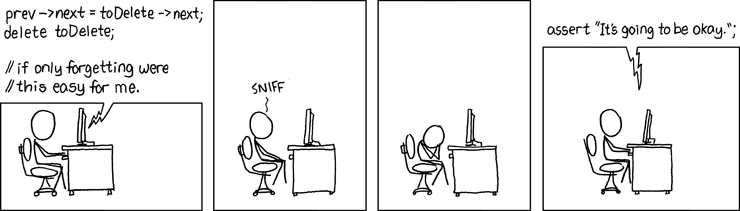
\includegraphics[width=\textwidth]{forgetting}
	\caption[]{\texttt{xkcd no.\ 379}}
	\label{fig:forgetting}
\end{figure}

\subsection{Pila}

La pila è una struttura dati \emph{dinamica}, \emph{lineare} in cui l'elemento rimosso dall'operazione di cancellazione è predeterminato, ed è quello che \enquote{è rimasto per meno tempo nell'insieme} (con strategia \textsc{LIFO}, \foreign{Last-In-First-Out}).

\begin{algorithm}[H]
	\caption[Specifica pila]{Specifica \textsc{Stack}}
	%&../preamble

% arara: pdflatex: { synctex: no }
% arara: latexmk: { clean: partial }
\ifstandalone
\begin{document}
\begin{algorithm}[H]
\fi

\Bool \stackEmpty \Comment*[r]{restituisce vero se la pila è vuota}
\stackPush{\Item \(v\)} \Comment*[r]{inserisce \(v\) in cima alla pila}
\Item \stackPop \Comment*[r]{estrae l'elemento in cima alla pila e lo restituisce al chiamante}
\Item \stackTop \Comment*[r]{legge l'elemento in cima alla pila}

\ifstandalone
\end{algorithm}
\end{document}
\fi

\end{algorithm}

Ogni volta che viene effettuata una chiamata a funzione si usa implicitamente una pila, che memorizza tutti i record di attivazione delle chiamate effettuate.
Sfrutteremo questo meccanismo implicito per visitare gli alberi, attraverso una visita in profondità.

Le pile possono essere implementate come:
\begin{itemize}
	\item liste bidirezionali, dove il puntatore punta all'elemento \textsf{top} (non utilizzate);
	\item tramite vettore, dove la dimesione è limitata quindi si crea un \foreign{overhead} più basso.
\end{itemize}

\begin{algorithm}[H]
	\caption{Struttura dati pila basata su vettore in pseudocodice}
	%&../preamble

% arara: pdflatex: { synctex: no }
% arara: latexmk: { clean: partial }
\ifstandalone
\begin{document}
\begin{algorithm}[H]
\fi
\begin{minipage}[t]{.45\textwidth}

% \BlankLine
\Item{} \(A\)	\Comment*[r]{elementi}
\Int \(n\)		\Comment*[r]{cursore}
\Int \(m\)		\Comment*[r]{dimesione massima}

\BlankLine
\tcp{crea una pila vuota}
\prototype{\Stack \stackConstructor{\Int dim}}{
	\Stack \(t =\) \new \Stack\;
	\(t.A =\) \new \Array{\Int}[0][dim-1]\;
	\(t.m = dim\)\;
	\(t.n = 0\)\;

	\BlankLine
	\Return \(t\)\;
}

\BlankLine
\tcp{leggi l'elemento in cima alla pila}
\prototype{\Item \stackTop}{
	\precondition{\(n > 0\)}

	\BlankLine
	\Return A[n]\;
}

% \vspace{10pt}
\end{minipage}\hfill%
\begin{minipage}[t]{.45\textwidth}
% \BlankLine
\tcp{restituisce \True se la pila è vuota}
\prototype{\Bool \stackEmpty}{
	\Return \(n \Equal 0\)
}

\BlankLine
\tcp{estrae l'elemento in cima alla pila e lo restituisce al chiamante}
\prototype{\Item \stackPop}{
	\precondition{\(n > 0\)}

	\BlankLine
	\Item \(t = A[n]\)\;
	\Decrement{n}\;

	\BlankLine
	\Return \(t\)
}

\BlankLine
\tcp{inserisce \(v\) in cima alla pila}
\prototype{\stackPush{\Item v}}{
	\precondition{\(n < m\)}

	\BlankLine
	\Increment{n}\;
	\(A[n] = v\)
}

\vphantom{0pt}

\end{minipage}
\ifstandalone
\end{algorithm}
\end{document}
\fi

\end{algorithm}

\begin{code}
	\captionof{listing}{Pila basata su vettore circolare in Java}
	\label{code:vector-stack}
	\pathinputminted{java}{VectorStack.java}
\end{code}

\clearpage
\subsection{Coda}

La coda è una struttura dati \emph{dinamica} \emph{lineare} in cui l'elemento rimosso dall'operazione di cancellazione è predeterminato, ed è quello che \enquote{è rimasto per più tempo nell'insieme} (con strategia, \textsc{FIFO}, \foreign{First-In-First-Out}).

\begin{algorithm}[H]
	\caption[Specifica coda]{Specifica \textsc{Queue}}
	%&../preamble

% arara: pdflatex: { synctex: no }
% arara: latexmk: { clean: partial }
\ifstandalone
\begin{document}
\begin{algorithm}[H]
\fi

\Bool \queueEmpty \Comment*[r]{restituisce vero se la coda è vuota}
\Item \queueInsert{\Item \(v\)} \Comment*[r]{inserisce \(v\) in fondo alla coda}
\Item \queueRemove \Comment*[r]{estrae l'elemento in cima alla coda e lo restituisce al chiamante}
\Item \queueTop \Comment*[r]{legge l'elemento in testa alla coda}

\ifstandalone
\end{algorithm}
\end{document}
\fi

\end{algorithm}

Nei sistemi operativi, i processi in attesa di utilizzare una risorsa vengono gestiti tramite una coda.
La politica \textsc{FIFO} è onesta (\foreign{fair}) rispetto l'ordine in cui i processi sono stati inseriti.

Le code possono essere implementate come:
\begin{itemize}
	\item liste monodirezionali, dove sono presenti due puntatori: uno alla testa (\foreign{head}) per l'estrazione, ed uno alla coda per l'inserimento;
	\item vettori circolari, il quale ha una dimensione limitata e crea un \foreign{overhead} più basso.
\end{itemize}

\begin{algorithm}[H][ht]
	\caption{Struttura dati coda basata su vettore circolare in pseudocodice}
	%&../preamble

% arara: pdflatex: { synctex: no }
% arara: latexmk: { clean: partial }
\ifstandalone
\begin{document}
\begin{algorithm}[H]
\fi
\begin{minipage}[t]{.45\textwidth}

\Item{} \(A\)	\Comment*[r]{elementi}
\Int \(n\)		\Comment*[r]{dimensione attuale}
\Int \(testa\)	\Comment*[r]{testa}
\Int \(m\)		\Comment*[r]{dimesione massima}

\BlankLine
\tcp{crea una cosa vuota}
\prototype{\Queue \queueConstructor{\Int dim}}{
	\Queue \(t =\) \new \Queue\;
	\(t.A =\) \new \Array{\Int}[0][dim-1]\;
	\(t.m = dim\)\;
	\(t.testa = 0\)\;
	\(t.n = 0\)\;

	\BlankLine
	\Return \(t\)\;
}

\BlankLine
\tcp{legge l'elemento in testa alla coda}
\prototype{\Item \queueTop}{
	\precondition{\(n > 0\)}

	\BlankLine
	\Return A[testa]\;
}

% \vspace{5pt}
\end{minipage}\hfill%
\begin{minipage}[t]{.45\textwidth}

% \BlankLine
\tcp{restituisce \True de la coda è vuota}
\prototype{\Item \queueEmpty}{
	\Return \(n \Equal 0\)\;
}

\BlankLine
\tcp{estrae l'elemento in testa alla coda e lo restituisce al chiamante}
\prototype{\Item \queueRemove}{
	\precondition{\(n > 0\)}

	\BlankLine
	\Item \(t = A[testa]\)\;
	\(testa = (testa+1) \bmod m\)\;
	\Decrement{n}\;

	\BlankLine
	\Return \(t\)\;
}

\BlankLine
\tcp{inserisce \(v\) in fondo alla coda}
\prototype{\Item \queueInsert}{
	\precondition{\(n < m\)}

	\BlankLine
	\(A[(testa+n) \bmod m]\) = \(v\)\;
	\Increment{n}\;
}

\vphantom{0pt}

\end{minipage}
\ifstandalone
\end{algorithm}
\end{document}
\fi

\end{algorithm}

\begin{figure}[hp]
\begin{code}
	\captionof{listing}{Coda basata su vettore in Java}
	\label{code:vector-queue}
	\pathinputminted{java}{VectorQueue.java}
\end{code}
\end{figure}

\ifsubfile
\end{document}
\fi

	%&../settings/preamble.main

\ifsubfile
\pagestyle{plain}
\setcounter{chapter}{4}

% NOTE sopprimere i warnings localmente
% \hbadness=10000
% \hfuzz=\maxdimen\newdimen\hfuzz
% % \usepackage[saveall]{silence}
% \usepackage{silence}
% \WarningsOff[caption]

% arara: pdflatex: { options: ["--output-directory=../build/chapters"], draft: yes, synctex: no }
% arara: pdflatex: { options: ["--output-directory=../build/chapters"], synctex: no }
\begin{document}
\fi
\chapter{Alberi}

% TODO scrivere introduzione

\section{Definizioni}

\begin{definition}[albero radicato, \foreign{rooted tree}]
Un albero consiste di un insieme di nodi e un insieme di archi orientati che connettono coppie di nodi, con le seguenti proprietà:
\begin{itemize}
	\item un nodo dell'albero è designato come nodo radice;
	\item ogni nodo \(n\), a parte la radice, ha esattamente un arco entrante;
	\item esiste un cammino unico dalla radice ad ogni nodo;
	\item l'albero è connesso.
\end{itemize}
\end{definition}

\begin{definition}[albero radicato, definizione ricorsiva]
Un albero è dato da:
\begin{itemize}
	\item un insieme vuoto, oppure
	\item una radice e zero o più sottoalberi, ognuno dei quali è albero; la radice è connessa alla radice di ogni sottoalbero con un arco orientato.
\end{itemize}
\end{definition}

\begin{definition}[profondità, \foreign{depth}]
La lunghezza del cammino semplice dalla radice al nodo (misurato in archi).
\end{definition}

\begin{definition}[livello, \foreign{level}]
L'insieme dei nodi alla stessa profondità.
\end{definition}

\begin{definition}[altezza dell'albero, \foreign{height}]
La profondità massima delle sue foglie.
\end{definition}

\section{Terminologia}

\begin{minipage}[c]{.45\textwidth}
	\centering
	\begin{itemize}[itemsep=5pt]
		\item \(A\) è la radice (\foreign{root});
		\item \(B\), \(C\) sono radici dei sottoalberi (\foreign{roots of their subtrees});
		\item \(D\), \(E\) sono fratelli (\foreign{siblings});
		\item \(D\), \(E\) sono figli (\foreign{children}) di \(B\);
		\item \(B\) è il padre (\foreign{parent}) di \(D\), \(E\);
		\item \(H\), \(I\), \(J\), \(K\), \(L\), \(M\), \(G\) sono foglie (\foreign{leafs});
		\item gli altri nodi sono nodi interni (\foreign{internal nodes});
		\item \(E\) è lo zio (il fratello del padre) di \(I\);
		\item \(B\) è il nonno di \(I\), \(I\) è il nipote di \(B\).
		% \item \(A\) è il bis-nonno di \(I\).
	\end{itemize}
\end{minipage}%
\begin{minipage}[c]{.45\textwidth}
	\centering
	\scalebox{.9}{
		\begin{forest} circled, wide
			[A [B [D [H][I]] [E [J][K]] ] [C [F [L][M]] [G] ]]
		\end{forest}
	}
\end{minipage}

\clearpage
\section{Alberi binari}

\begin{definition}[Albero binario]
Un albero binario è un albero radicato in cui ogni nodo ha al massimo due figli, che vengono identificati come figlio sinistro e figlio destro.
\end{definition}

\begin{note}
Due alberi \(T\) e \(U\) che hanno gli stessi nodi, gli stessi figli per ogni nodo e la stessa radice, sono distinti qualora un nodo \(u\) sia designato come figlio sinistro di un nodo \(v\) in \(T\) come figlio destro del medesimo nodo in \(U\).
In altre parole, anche se due alberi hanno lo stesso numero di nodi ed ognuno di questi nodi ha lo stesso numero di figli non è che detto che l'albero risultante sia identico.
\end{note}

\begin{algorithm}[H]
\caption*{Specifica albero binario}
%&../preamble

% arara: pdflatex: { synctex: no }
% arara: latexmk: { clean: partial }
\ifstandalone
\begin{document}
\begin{algorithm}[H]
\fi

\BlankLine
\tcp{GESTIONE ALBERO}

\BlankLine
\treeConstructor{\Item \(v\)} \Comment*[l]{costruisce un nuovo nodo, contenente \(v\), senza figli o genitori}
\Item \treeRead \Comment*[l]{legge il valore memorizzato nel nodo}
\treeWrite{\Item \(v\)} \Comment*[l]{modifica il valore memorizzato nel nodo}
\Tree \treeParent \Comment*[l]{restituisce il padre, oppure \Nil se questo nodo è radice}

\BlankLine
\BlankLine
\tcp{GESTIONE STRUTTURA}

\BlankLine
\tcp{restituiscono il figlio sinistro (destro) di questo nodo,}
\tcp{restituisce \Nil se assente}
\Tree \treeLeft\;
\Tree \treeRight\;

\BlankLine
\tcp{inserisce il sottoalbero radicato in \(t\)}
\tcp{come figlio sinistro (destro) di questo nodo}
\insertLeft{\Tree \(t\)}\;
\insertRight{\Tree \(t\)}\;

\BlankLine
\tcp{distrugge (ricorsivamente) il figlio sinistro (destro) di questo nodo}
\deleteLeft\;
\deleteRight\;

\ifstandalone
\end{algorithm}
\end{document}
\fi

\end{algorithm}

\begin{note}
Le funzioni \emph{senza parametri} sono indicate con un carattere senza grazie e privi di parentesi tonde vuote al fine di alleggerire la lettura del codice.
\end{note}

\subsection{Memorizzazione di un albero binario}

\begin{figure}[H]
	\centering
	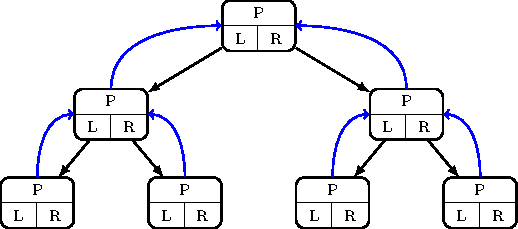
\includegraphics{tree-binary}
\end{figure}

Vengono memorizzati i seguenti campi:
\begin{itemize}
	\item \emph{parent}: riferimento al nodo padre;
	\item \emph{left}: riferimento al figlio sinistro;
	\item \emph{right}: riferimento al figlio destro.
\end{itemize}
Uno qualunque di questi oggetti potrebbe essere pari a \Nil, stando ad indicare che non esiste nessun sottoalbero.

\subsection{Implementazione}

\begin{algorithm}[H]
	\caption{Implementazione albero binario in pseudocodice}
	%&../preamble

% arara: pdflatex: { synctex: no }
% arara: latexmk: { clean: partial }
\ifstandalone
\begin{document}
\begin{algorithm}[H]
\fi
\begin{minipage}[t]{.5\textwidth}

\tcp{crea un nuovo albero}
\tcp{restituisce la radice dell'albero creato}
\prototype{\Tree \treeConstructor{\Item \(v\)}}{
	\Tree \(t =\) \new \Tree\;
	\(t.\varParent \Assign \Nil\)\;
	\(t.\varLeft \Assign t.\varRight \Assign \Nil\)\;
	\(t.\Value \Assign v\)\;

	\BlankLine
	\Return \(t\)\;
}

\prototype{\insertLeft{\Tree \(t\)}}{
	\If{\(\varLeft \Neq \Nil\)}{
		\(t.\varParent \Assign \This\)\;
		\(\varLeft \Assign t\)\;
	}
}

\prototype{\insertRight{\Tree \(t\)}}{
	\If{\(\varRight \Neq \Nil\)}{
		\(t.\varParent \Assign \This\)\;
		\(\varRight \Assign t\)\;
	}
}

\end{minipage}% <- importante, non toccare!
\begin{minipage}[t]{.5\textwidth}

\tcp{elimina ricorsivamente il sottoalbero sinistro}
\prototype{\deleteLeft{}}{
	\If{\(\varLeft \Neq \Nil\)}{
		\(\varLeft.\deleteLeft\)\;
		\(\varLeft.\deleteRight\)\;
		\(\varLeft \Assign \Nil\)\;
	}
}

\tcp{elimina ricorsivamente il sottoalbero destro}
\prototype{\deleteRight{}}{
	\If{\(\varRight \Neq \Nil\)}{
		\(\varRight.\deleteLeft\)\;
		\(\varRight.\deleteRight\)\;
		\(\varRight \Assign \Nil\)\;
	}
}

\end{minipage}
\ifstandalone
\end{algorithm}
\end{document}
\fi

\end{algorithm}

\subsection{Visite}

La visita di un albero (o la ricerca) è una strategia per passare attraverso (visitare) tutti i nodi di un albero.
Si possono distinguere due tipi di visite:
\begin{enumerate}
	\item visita in profondità: chiamata anche \foreign{Depth-First Search} (DFS), per visitare un albero visita ricorsivamente ognuno dei suoi sottoalberi; esistono tre varianti in base a quando il nodo viene visitato (pre, in o post-ordine); questa particolare visita sfrutta implicitamente il meccanismo di una pila (\foreign{stack}) tramite le chiamate ricorsive effettuate;
	\item visita in ampiezza: chiamata anche \foreign{Breadth First Search} (BFS), per visitare un albero visita ogni livello, uno dopo l'altro partendo dalla radice; richiede esplicitamente l'utilizzo di una coda (\foreign{queue}).
\end{enumerate}

\begin{algorithm}[H]
	\caption{Schema per visita in profondità}
	%&../preamble

% arara: pdflatex: { synctex: no }
% arara: latexmk: { clean: partial }
\ifstandalone
\begin{document}
\begin{algorithm}[H]
\fi
\begin{minipage}[t]{.5\linewidth}

\BlankLine
\prototype{\dfsSchema{\Tree \(t\)}}{
	\If{\(t \neq \Nil\)}{

		\BlankLine
		\tcp{pre-order visit}
		\Print \(t\)\;

		\BlankLine
		\dfsProc{\(t.\treeLeft\)}\;

		\BlankLine
		\tcp{in-order visit}
		\Print \(t\)\;

		\BlankLine
		\dfsProc{\(t.\treeRight\)}\;

		\BlankLine
		\tcp{post-order visit}
		\Print \(t\)\;
	}
}

\end{minipage}%
\begin{minipage}[t]{.5\linewidth}

\ifFigureOfAlgo
\begin{minipage}[t][5cm]{.5\linewidth}
	\centering
	\vfill
	\begin{forest} circled, for tree={font=\footnotesize\scshape}
		[a
			[b
				[c]
				[d]
			]
			[e
				[f]
				[g]
			]
		]
	\end{forest}
	\vfill
	\begin{tabular}{@{} l *{7}{ >{\scshape}c @{} } @{}}\small
		\emph{pre}-visita  & a & b & c & d & e & f & g \\
		\emph{in}-visita   & c & b & d & a & f & e & g \\
		\emph{post}-visita & c & d & b & f & g & e & a \\
	\end{tabular}
\end{minipage}
\fi

\end{minipage}
\ifstandalone
\end{algorithm}
\end{document}
\fi

\end{algorithm}

A seconda di dove scrivo il codice in questo schema ottengo una visita diversa.

\clearpage
\subsection{Applicazioni}

In genere post-visita e in-visita sono quelle più applicate, la pre-visita meno.

\subsection*{Visita in post-ordine}

Una possibile applicazione della visita post-ordine è quella di effettuare un conteggio dei nodi presenti nell'albero.

\begin{algorithm}[H]
	\caption{Conteggio dei nodi in un albero}
	%&../preamble

% arara: pdflatex: { synctex: no }
% arara: latexmk: { clean: partial }
\ifstandalone
\begin{document}
\begin{algorithm}[H]
\fi
\begin{minipage}[c]{.4\textwidth}

\prototype{\conteggioNodi{\Tree \(t\)}}{
	\eIf{\(t \Equal \Nil\)}{
		\tcp{è un albero vuoto}
		\Return \(0\)\;
	}{
		\tcp{conto ricorsivamente i nodi}
		\(C_{\ell} = \conteggioNodi{\(t.\treeLeft\)}\)\;
		\(C_{r} = \conteggioNodi{\(t.\treeRight\)}\)\;

		\BlankLine
		\Return \(C_{\ell} + C_{r} + 1\)\;
	}
}

\end{minipage}%
\begin{minipage}[c]{.5\textwidth}%
\ifFigureOfAlgo%
\hfill% centramento orizzontale
\begin{minipage}[t][3.8cm]{.85\linewidth}
	\centering
	\begin{forest} circled, wide,
		for tree={
			font=\scshape,
			count/.style 2 args={
				edge label={node[near end, font=\sffamily\scriptsize, #1]{#2}},
		    },
		}
		[a
			[b, count={above left}{3}
				[c, count={above left}{1}]
				[d, count={above right}{1}]
			]
			[e, count={above right}{3}
				[f, count={above left}{1}]
				[g, count={above right}{1}]
			]
		]
	\end{forest}
\end{minipage}
\fi
\end{minipage}
\ifstandalone
\end{algorithm}
\end{document}
\fi

\end{algorithm}

\subsection*{Visita in ordine (in-visita)}

Una possibile applicazione della visita post-ordine è quella di stampare espressioni con operatori binari.

\begin{algorithm}[H]
	\caption{Stampa espressioni con operatori binari}
	%&../preamble

% arara: pdflatex: { synctex: no }
% arara: latexmk: { clean: partial }
\ifstandalone
\begin{document}
\begin{algorithm}[H]
\fi
\begin{minipage}{.5\textwidth}

\prototype{\Int \stampaEspressioni{\Tree \(t\)}}{
	\eIf{\(t.\treeLeft \Equal \Nil\) \And \(t.\treeRight \Equal \Nil\)}{
		\tcp{siamo in una foglia}
		\Print \(t.\treeRead\)
	}{
		\tcp{sono su un nodo interno}
		\Print \enquote{(}\;

		\stampaEspressioni{\(t.\treeLeft\)}\;

		\Print \(t.\treeRead\)\;

		\stampaEspressioni{\(t.\treeRight\)}\;

		\Print \enquote{)}\;
	}
}

\end{minipage}%
\begin{minipage}{.5\textwidth}
\ifFigureOfAlgo
\begin{minipage}[t][4.5cm]{.85\linewidth}
	\vfill\centering
	\begin{center}
		\begin{forest} circled math tree
		[*[+[4][9]][+[3][4]]]
		\end{forest}
	\end{center}
	Stampa: \texttt{(( 4 + 9 ) * ( 3 + 4 ))}
	\vfill
\end{minipage}
\fi

\end{minipage}
\ifstandalone
\end{algorithm}
\end{document}
\fi

\end{algorithm}

% TODO
% Questa particolare funzione è stata utilizzata nell'esame del

\subsection*{Complessità di una visita}

Il costo di una visita di un albero contenente \(n\) nodi è \(\Theta(n)\), in quanto ogni nodo viene visitato al massimo una volta.

\clearpage
\section{Alberi generici}

\begin{algorithm}[H]
	\caption{Specifica albero generico}
	%&../preamble

% arara: pdflatex: { synctex: no }
% arara: latexmk: { clean: partial }
\ifstandalone
\begin{document}
\begin{algorithm}[H]
\fi

\BlankLine
\tcp{GESTIONE ALBERO}

\BlankLine
\treeConstructor{\Item \(v\)} \Comment*[l]{costruisce un nuovo nodo, contenente \(v\), senza figli o genitori}
\Item \treeRead \Comment*[l]{legge il valore memorizzato nel nodo}
\treeWrite{\Item \(v\)} \Comment*[l]{modifica il valore memorizzato nel nodo}
\Tree \treeParent \Comment*[l]{restituisce il padre, oppure \Nil se questo nodo è radice}

\BlankLine
\BlankLine
\tcp{GESTIONE STRUTTURA}

\begin{minipage}{\textwidth}%
\begin{multicols}{2}%

\BlankLine
\tcp{restituiscono il primo figlio,}
\tcp{oppure \Nil se questo nodo è una foglia}
\Tree \treeChild\;

\BlankLine
\tcp{restituisce il prossimo fratello,}
\tcp{oppure \Nil se assente}
\Tree \treeSibling\;

\BlankLine
\tcp{inserisce il sottoalbero \(t\)}
\tcp{come primo figlio di questo nodo}
\insertChild{\Tree \(t\)}

\BlankLine
\tcp{inserisce il sottoalbero \(t\)}
\tcp{come prossimo fratello di questo nodo}
\insertSibling{\Tree \(t\)}

\BlankLine
\tcp{distuggi l'albero radicato}
\tcp{identificato dal primo fratello}
\deleteChild

\BlankLine
\tcp{distuggi l'albero radicato}
\tcp{identificato dal primo figlio}
\deleteSibling

\end{multicols}
\end{minipage}
\vspace{5pt}

\ifstandalone
\end{algorithm}
\end{document}
\fi

\end{algorithm}

\subsection{Visita in profondità}

Un albero binario è anche un albero generale e lo visitiamo esattamente come lo visitavamo prima.

\begin{algorithm}[H]
	\caption{Visita in profondità}
	%&../preamble

% arara: pdflatex: { synctex: no }
% arara: latexmk: { clean: partial }
\ifstandalone
\begin{document}
\begin{algorithm}[H]
\fi

\BlankLine
\prototype{\dfsProc{\Tree \(t\)}}{
	\If{\(t \neq \Nil\)}{

		\BlankLine
		\tcp{pre-order visit}
		\Print \(t\)\;

		\BlankLine
		\dfsProc{\(t.\treeLeft{}\)}\;

		\BlankLine
		\tcp{effettuo visita}
		\Tree \(u\) \Assign \(t\).\treeChild\;
		\While{\(u \Neq \Nil\)}{
			\dfsProc{\(u\)}\;
			\(u\).\treeSibling\;
		}

		\BlankLine
		\tcp{post-order visit}
		\Print \(t\)\;
	}
}

\ifstandalone
\end{algorithm}
\end{document}
\fi

\end{algorithm}

\subsection{Visita in ampiezza}

Mentre nella visita in profondità il meccanismo della pila (\foreign{stack}) era implicito nelle chiamate ricorsive, in questo caso è necessario utilizzare \emph{esplicitamente} una coda (\foreign{queue}).
Un'altra differenza fra i due algoritmi è che quello in profondità è un algoritmo ricorsivo, l'altro è iterativo.
Quando tutti i nodi di un livello vengono estratti dalla coda, la coda contiene solo ed unicamente i nodi del livello successivo.

\begin{algorithm}[H]
	\caption{Visita in ampiezza}
	%&../preamble

% arara: pdflatex: { synctex: no }
% arara: latexmk: { clean: partial }
\ifstandalone
\begin{document}
\begin{algorithm}[H]
\fi
\begin{minipage}{.5\textwidth}

\prototype{\bfsProc{\Tree \(t\)}}{
	\Queue \(Q \Assign\) \queueConstructor\;
	\(Q.\queueInsert{t}\) \Comment*[l]{inserisci la radice}

	\BlankLine
	\While{\Not \(Q.\queueEmpty\)}{
		\tcp{fintanto che la coda non è vuota}
		\tcp{estraggo un nodo dalla coda}
		\Tree \(u \Assign Q.\queueRemove\)\;

		\BlankLine
		\tcp{visita per livelli del nodo \(u\)}
		\Print \(u\)\;

		\BlankLine
		\tcp{fintanto che ho almeno un figlio}
		\(u \Assign u.\treeChild\)\;
		\While{\(u \Neq \Nil\)}{

			\BlankLine
			\tcp{metto in coda il figlio}
			\(Q.\queueInsert{u}\)\;
			\tcp{passo al figlio destro}
			\(u \Assign u.\treeSibling\)\;
		}
	}
}

\end{minipage}%
\begin{minipage}{.5\textwidth}

\ifFigureOfAlgo
\begin{minipage}[t][7.5cm]{.85\linewidth}
	\vfill\centering
	\begin{center}
		\begin{forest} circled, wide
		[\textsc{a}[\textsc{b}[\textsc{c}][\textsc{d}]][\textsc{e}[\textsc{f}][\textsc{g}]]]
		\end{forest}
	\end{center}
	Sequenza: {\scshape a b e c d f g}
	\vfill\null
\end{minipage}
\fi

\end{minipage}
\ifstandalone
\end{algorithm}
\end{document}
\fi

\end{algorithm}

\paragraph{Commento}
Mettiamo in coda tutti i nodi che vogliamo visitare passo passo.
Qui la stampa è in pre-visita ma qui -- a differenza dei grafi -- non ha molta importanza se la visita la facciamo prima o dopo.
Visito tutti i figli prima di passare al livello successivo.

\section{Memorizzazione}

Esistono diversi modi per memorizzare un albero, più o meno indicati a seconda del numero massimo e medio di figli presenti.
Le realizzazioni possibili sono:
\begin{enumerate}
	\item con vettore dei figli;
	\item primo figlio, prossimo fratello;
	\item con vettore dei padri
\end{enumerate}

\subsection{Realizzazione con vettore dei figli}

\begin{figure}[H]
	\centering
	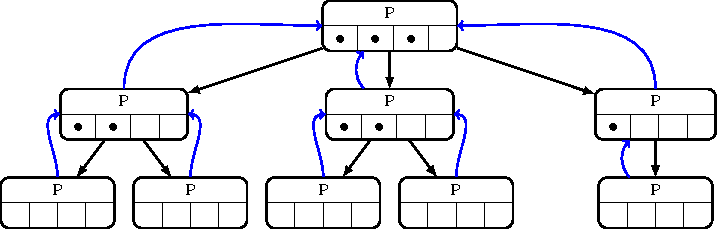
\includegraphics[width=.8\textwidth]{tree-vectorChildren}
	\caption[Realizzazione di un albero tramite vettore dei figli]{Realizzazione con vettore dei figli}
	\label{fig:tree-vector-children}
\end{figure}

Vengono memorizzati i seguenti campi:
\begin{itemize}
	\item \emph{parent} che è il riferimento al nodo padre;
	\item vettore dei figli il quale a seconda del numero dei figli può comportare una discreta quantità di spazio sprecato.
\end{itemize}

\subsection{Realizzazione basata su primo figlio, prossimo fratello}

Viene implementato come una lista di fratelli.

\begin{figure}[H]
	\centering
	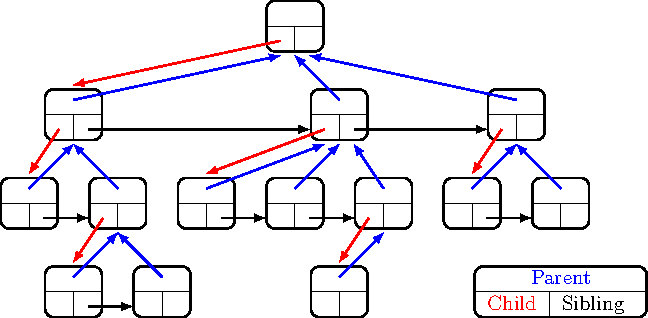
\includegraphics[width=.8\textwidth]{tree-listChildren}
	\caption[Realizzazione di un albero tramite primo figlio, prossimo fratello]{Realizzazione basata su primo figlio, prossimo fratello}
	\label{fig:tree-list-children}
\end{figure}

La memorizzazione che viene utilizzata nel \foreign{file system} è esattamente questa.

\begin{algorithm}[H]
	\caption{Implementazione albero \enquote{primo figlio, prossimo fratello} in pseudocodice}
	%&../preamble

% arara: pdflatex: { synctex: no }
% arara: latexmk: { clean: partial }
\ifstandalone
\begin{document}
\begin{algorithm}[H]
\fi

\Tree \varParent \Comment*[r]{Riferimento al padre}
\Tree \varChild \Comment*[r]{Riferimento al primo figlio}
\Tree \varSibling \Comment*[r]{Riferimento al prossimo fratello}
\Item \varValue \Comment*[r]{Valore memorizzato nel nodo}

\begin{minipage}{.5\textwidth}

\BlankLine
\prototype{\Tree \treeConstructor{\Item \(v\)}}{
	\Tree \(t =\) \new \Tree\;
	\(t.\varValue \Assign v\)\;
	\(t.\varParent \Assign t.\varChild \Assign t.\varSibling \Assign \Nil\)\;

	\BlankLine
	\Return \(t\)\;
}

\BlankLine
\prototype{\insertChild{\Tree \(t\)}}{
	\(t.\varParent \Assign \Self\)\;
	\tcp{inserisci \(t\) prima dell'attuale primo figlio}
	\(t.\varSibling \Assign \varChild\)\;
	\(\varChild \Assign t\)\;
}

\BlankLine
\prototype{\insertSibling{\Tree \(t\)}}{
	\(t.\varParent \Assign \varParent\)\;
	\tcp{inserisci \(t\) prima dell'attuale prossimo fratello}
	\(t.\varSibling \Assign \varSibling\)\;
	\(\varSibling \Assign t\)\;
}

\end{minipage}%
\begin{minipage}{.5\textwidth}

\BlankLine
\prototype{\deleteChild{}}{
	\(\Tree\ newChild\ \Assign \varChild.\treeSibling\)\;
	\delete{\varChild}\;
	\(\varChild \Assign newChild\)\;
}

\BlankLine
\prototype{\deleteSibling{}}{
	\(\Tree\ newBrother\ \Assign \varSibling.\treeSibling\)\;
	\treeDelete{\varSibling}\;
	\(\varSibling \Assign newBrother\)\;
}

\BlankLine
\tcp{metodo ausiliare}
\prototype{\treeDelete{\Tree \(t\)}}{
	\Tree \(u\) \Assign \(t\).\treeChild\;

	\BlankLine
	\While{\(u \Neq \Nil\)}{
		\Tree \(next\) \Assign \(u\).\treeSibling\;
		\treeDelete{\(u\)}\;
		\(u \Assign next\)\;
	}
}

\end{minipage}

\ifstandalone
\end{algorithm}
\end{document}
\fi

\end{algorithm}

\newpage
\subsection{Realizzazione con vettore dei padri}

Nella realizzazione con vettore dei padri, l'albero è rappresentato da un vettore i cui elementi contengono il valore associato al nodo e l'indice della posizione del padre del vettore.

\bigskip
\begin{minipage}[c]{.5\textwidth}
	\centering
	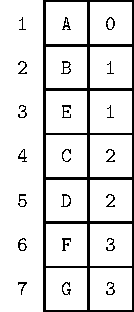
\includegraphics{tree-vectorParents}
\end{minipage}%
\begin{minipage}[c]{.5\textwidth}
	\centering
	\begin{forest} circled, wide, for tree={font=\scshape}
	[a[b[c][d]][e[f][g]]]
	\end{forest}
\end{minipage}

\bigskip
Questa realizzazione può sembrare particolarmente assurda poiché dato un nodo non permette di stabilire direttamente quali sono i suoi figli, ma ci sono molti algoritmi che sono interessati solo ai padri.
Questa è la rappresentazione più compatta che possiamo creare, vedremo la sua utilità quando andremo a studiare le visite sui grafi.

\ifsubfile
\end{document}
\fi

	%&../settings/preamble.main

\ifsubfile
\pagestyle{plain}
\setcounter{chapter}{5}

% arara: pdflatex: { options: ["--output-directory=../build"], draft: yes, synctex: no }
% arara: pdflatex: { options: ["--output-directory=../build"], synctex: no }
\begin{document}
\fi
\chapter{Alberi Binari di Ricerca}

\section{Introduzione}

Facciamo un breve ripasso della struttura dati dizionario.
La struttura dati dizionario è un insieme dinamico che implementa le seguenti funzionalità:
\begin{itemize}
	\item \Item \dictLookup{\Item \(v\)} permette di cercare per una certa chiave;
	\item \dictInsert{\Item \(k\), \Item \(v\)} permette di associare una chiave ad un valore;
	\item \dictRemove{\Item \(k\)} permette di rimuovere una certa associazione chiave-valore.
\end{itemize}

\begin{table}[H]
	\centering
	% \captionsetup{format=hang}
	\caption{Possibili implementazioni della struttura dati dizionario\\e relative complessità}
	\label{tab:complessita-implementazioni-dizionario}
	\begin{tabular}{@{} l *{3}{c} @{}}
	\toprule
		Struttura dati & \dictLookup & \dictInsert & \dictRemove\\
	\midrule
	Vettore ordinato & \(\Omicron(\log n)\) & \(\Omicron(n)\) & \(\Omicron(n)\)\\
	Vettore non ordinato & \(\Omicron(n)\) & \({\Omicron(1)}^{*}\) & \({\Omicron(1)}^{*}\)\\
	Lista non ordinata & \(\Omicron(n)\) & \({\Omicron(1)}^{*}\) & \({\Omicron(1)}^{*}\)\\
	\bottomrule
	\end{tabular}

	\smallskip
	{\small	* assumendo che l'elemento sia già stato trovato, \(\Omicron(n)\) altrimenti.}
\end{table}

Ora vedremo la struttura dati dizionario implementata come un albero binario di ricerca.

L'idea che ha portato allo sviluppo degli alberi binari di ricerca è stata quella di portare la ricerca binaria (o dicotomica) negli alberi, avendo quindi un meccanismo dinamico per la memorizzazione delle informazioni ma basandosi sul meccanismo della ricerca binaria per recuperarle.

Le associazioni chiave-valore vengono memorizzate in un albero binario.
Ogni nodo contiene una coppia (\(u\).\varKey, \(u\).\varValue).
Le chiavi devono appartenere ad un insieme \emph{totalmente ordinato}, ossia dev'essere possibile stabilire, date due chiavi, una relazione di precendenza fra di loro.

\begin{property*}
Le seguenti proprietà permettono di realizzare un algoritmo di ricerca dicotomica:
\begin{enumerate}
	\item Le chiavi contenute nei nodi del sottoalbero sinistro di \(u\) sono minori di \(u\).\varKey;
	\item Le chiavi contenute nei nodi del sottoalbero destro di \(u\) sono maggiori di \(u\).\varKey.
\end{enumerate}
\end{property*}

\begin{note}
Queste proprietà valgono per ogni nodo e riguardano l'intero sottoalbero.
\end{note}

Vedremo un algoritmo per verificare se un albero binario è un albero binario di ricerca più avanti (\verifyABR), il quale controllerà se queste proprietà sono soddisfatte.

\clearpage
\begin{algorithm}[H]
	\caption*{Specifica Alberi Binari di Ricerca (\textsc{ABR})}
	%&../preamble

% arara: pdflatex: { synctex: no }
% arara: latexmk: { clean: partial }
\ifstandalone
\begin{document}
\begin{algorithm}[H]
\fi

\begin{minipage}[t]{.45\textwidth}
\BlankLine
\tcp{CONTENUTO DI UN NODO}

\BlankLine
\Tree \varParent\;
\Tree \varLeft\;
\Tree \varRight\;
\Item \varKey\;
\Item \varValue\;

\BlankLine
\tcp{GETTERS}

\BlankLine
\Tree \treeParent\;
\Tree \treeLeft\;
\Tree \treeRight\;
\Item \treeKey\;
\Item \treeValue\;

% \columnbreak
% \vspace{15pt}
% \vphantom{0pt}
\end{minipage}\hfill%
\begin{minipage}[t]{.45\textwidth}

\BlankLine
\tcp{ORDINAMENTO}

\BlankLine
\Tree \succNode{\Tree \(t\)}\;
\Tree \predNode{\Tree \(t\)}\;
\Tree \minNode\;
\Tree \maxNode\;

\BlankLine
\tcp{FUNZIONI DIZIONARIO}

\BlankLine
\Item \dictLookup{\Item \(k\)}\;
\dictInsert{\Item \(k\), \Item \(v\)}\;
\dictRemove{\Item \(k\)}\;

\BlankLine
\tcp{FUNZIONI INTERNE}

\BlankLine
\Item \lookupNode\;
\insertNode{\Tree \(T\), \Item \(k\), \Item \(v\)}\;
\removeNode{\Tree \(T\), \Item \(k\)}\;
\end{minipage}
\BlankLine

\ifstandalone
\end{algorithm}
\end{document}
\fi

\end{algorithm}

\subsection*{Ricerca di un nodo}

\begin{algorithm}[H]
	\caption{Ricerca di un nodo in un dizionario realizzato tramite \textsc{ABR}}
	%&../preamble

% arara: pdflatex: { synctex: no }
% arara: latexmk: { clean: partial }
\ifstandalone
\begin{document}
\begin{algorithm}[H]
\fi

\BlankLine
\prototype{\Int \dictLookup{\Item \(k\)}}{
	\Tree \(t\) \Assign \lookupNode{\(tree, k\)}\;

	\BlankLine
	\eIf{\(t \Neq \Nil\)}{
		\Return \(t\).\treeValue\;
	}{
		\Return \Nil\;
	}
}

\BlankLine
% \tcp{Restituisce il nodo dell'albero \(t\)}
% \tcp{che contiene la chiave \(k\),}
% \tcp{se presente, \Nil altrimenti}
\tcp{RICERCA DI UN NODO, iterativa}
\prototype{\Tree \lookupNode{\Tree \(T\), \Item \(k\)}}{
	\Tree \(u \Assign T\) \Comment*[l]{parto dalla radice}

	\BlankLine
	\While{\(u \Neq \Nil\) \And \(u.\treeKey \Neq k\)}{
		\(u\) \Assign \iif{\(k < u.\treeKey, u.\treeLeft, u.\treeRight\)}\;
	}
}

\BlankLine
\tcp{RICERCA DI UN NODO, ricorsiva}
\prototype{\Tree \lookupNode{\Tree \(T\), \Item \(k\)}}{
	\eIf{\(T \Equal \Nil\) \Or \(T.\treeKey \Equal k\)}{
		\Return \(T\)\;
	}{
		\Return \lookupNode{\iif{\(k < u.\treeKey, u.\treeLeft, u.\treeRight\)}, \(k\)}\;
	}
}
\BlankLine

\ifstandalone
\end{algorithm}
\end{document}
\fi

\end{algorithm}

\clearpage
\subsection*{Ricerca del minimo e del massimo}

\begin{algorithm}[H]
	\caption{Ricerca del minimo e del massimo in un dizionario realizzato tramite \textsc{ABR}}
	%&../preamble

% arara: pdflatex: { synctex: no }
% arara: latexmk: { clean: partial }
\ifstandalone
\begin{document}
\begin{algorithm}[H]
\fi

\begin{minipage}{.5\textwidth}
\BlankLine
\tcp{RICERCA DEL MINIMO}
\prototype{\Tree \minNode{\Tree \(T\)}}{
	\Tree \(u = T\) \Comment*[l]{parto dalla radice}

	\BlankLine
	\While{\(u.\treeLeft \Neq \Nil\)}{
		\(u \Assign u.\treeLeft\)\;
	}

	\BlankLine
	\Return \(u\)\;
}

% \vspace{-5pt}
% \vphantom{0pt}
\end{minipage}%
\begin{minipage}{.5\textwidth}

\BlankLine
\tcp{RICERCA DEL MASSIMO}
\prototype{\Tree \maxNode{\Tree \(T\)}}{
	\Tree \(u = T\) \Comment*[l]{parto dalla radice}

	\BlankLine
	\While{\(u.\treeRight \Neq \Nil\)}{
		\(u \Assign u.\treeRight\)\;
	}

	\BlankLine
	\Return \(u\)\;
}
\end{minipage}
\BlankLine

\ifstandalone
\end{algorithm}
\end{document}
\fi

\end{algorithm}

\subsection*{Ricerca del predecessore, successore}

\begin{algorithm}[H]
	\caption{Ricerca del predecessore e del successore di un nodo in un dizionario realizzato tramite \textsc{ABR}}
	%&../preamble

% arara: pdflatex: { synctex: no }
% arara: latexmk: { clean: partial }
\ifstandalone
\begin{document}
\begin{algorithm}[H]
\fi

\begin{minipage}{.5\textwidth}
\BlankLine
\tcp{RICERCA DEL PREDECESSORE}
\prototype{\Tree \predNode{\Tree \(t\)}}{

	\BlankLine
	\If{\(t \Equal \Nil\)}{
		\Return \(t\)\;
	}

	\BlankLine
	\eIf{\(t.\alert{\treeLeft} \Neq \Nil\)}{
	\lnlset{sx-does-exists}{1}%
		\Return \(\alert{\maxNode{t.\treeLeft}}\)\;
	}{\lnlset{sx-not-exists}{2}%
		\Tree \(p \Assign t.\treeParent\)\;

		\BlankLine
		\While{\(p \Neq \Nil\) \And \(t \Equal p.\alert{\treeLeft}\)}{
			\(t \Assign p\) \Comment*[l]{padre}
			\(p \Assign p.\treeParent\) \Comment*[l]{nonno}
		}
	}

	\BlankLine
	\Return \(p\)\;
}

% \vspace{-5pt}
% \vphantom{0pt}
\end{minipage}%
\begin{minipage}{.5\textwidth}

\BlankLine
\tcp{RICERCA DEL SUCCESSORE}
\prototype{\Tree \succNode{\Tree \(t\)}}{

	\BlankLine
	\If{\(t \Equal \Nil\)}{
		\Return \(t\)\;
	}

	\BlankLine
	\eIf{\(t.\alert{\treeRight} \Neq \Nil\)}{
	\lnlset{dx-dies-exists}{3}%
		\Return \(\alert{\minNode{t.\alert{\treeRight}}}\)\;
	}{\lnlset{dx-not-exists}{4}%
		\Tree \(p \Assign t.\treeParent\)\;

		\BlankLine
		\While{\(p \Neq \Nil\) \And \(t \Equal p.\alert{\treeRight}\)}{
			\(t \Assign p\)\;
			\(p \Assign p.\treeParent\)\;
		}
	}

	\BlankLine
	\Return \(p\)\;
}
\end{minipage}
\BlankLine

\ifstandalone
\end{algorithm}
\end{document}
\fi

\end{algorithm}

\begin{enumerate}[label={\footnotesize\ttfamily (\arabic*)}]
	\item \(u\) ha figlio sinistro: il predecessore è il massimo del sottoalbero sinistro di \(u\);
	\item \(u\) non ha figlio sinistro: risalendo attraverso i padri, il predecessore è il primo avo \(v\) tale per cui \(u\) sta nel sottoalbero destro di \(v\);
	\item \(u\) ha figlio destro: il successore è il minimo del sottoalbero destro di \(u\);
	\item \(u\) non ha figlio destro: risalendo attraverso i padri, il sucessore è il primo avo \(v\) tale per cui \(u\) sta nel sottoalbero sinistro di \(v\).
\end{enumerate}

\begin{note}
Posso trovare \Nil se passo alla funzione \succNode il nodo massimo o alla funzione \predNode il minimo (usciranno dal ciclo restituendo \(p\) che sarà pari a \Nil).
\end{note}

\clearpage
\subsection*{Inserimento di un nodo}

La funzione \insertNode inserisce un'associazione chiave-valore \((k,v)\) nell'albero \(T\).
Se la chiave è già presente, sostituisce il valore associato;
altrimenti, viene inserita una nuova associazione.
Se l'albero è vuoto (\(T \Equal \Nil\)) restituisce il primo nodo dell'albero, altrimenti restituisce la radice di \(T\) inalterata.

La funzione ausiliaria \shortcut si occupa di inserire il nodo collegandolo al corretto genitore.

\begin{algorithm}[H]
	\caption{Inserimento di un nodo in un \textsc{Dictionary} realizzato tramite \textsc{ABR}}
	%&../preamble

% arara: pdflatex: { synctex: no }
% arara: latexmk: { clean: partial }
\ifstandalone
\begin{document}
\begin{algorithm}[H]
\fi

\BlankLine
\tcp{IMPLEMENTAZIONE DIZIONARIO}
\prototype{\dictInsert{\Item \(k\), \Item \(v\)}}{
	\(tree\) \Assign \insertNode{\(tree, k, v\)}\;
}

\ifstandalone
\end{algorithm}
\end{document}
\fi

	%&../preamble

% arara: pdflatex: { synctex: no }
% arara: latexmk: { clean: partial }
\ifstandalone
\begin{document}
\begin{algorithm}[H]
\fi

\BlankLine
\tcp{INSERIMENTO DI UN NODO}
\prototype{\Tree \insertNode{\Tree \(T\), \Item \(k\), \Item \(v\)}}{
	\Tree \(p \Assign \Nil\) \Comment*[l]{padre}
	\Tree \(u \Assign T\) \Comment*[l]{parto dalla radice}

	\BlankLine
	\tcp{cerco posizione inserimento}
	\While{\(u \Neq \Nil\) \And \(u.\treeKey \Neq k\)}{
		\(p \Assign u\)\;
		\(u\) \Assign \iif{\(k < u.\treeKey, u.\treeLeft, u.\treeRight\)}\;
	}

	\BlankLine
	\eIf{\(u \Neq \Nil\) \And \(u.\treeKey \Equal k\)}{
		\tcp{la chiave è già presente, aggiorno il valore}

		\BlankLine
		\(u.\treeValue \Assign v\)\;
	}{
		\tcp{la chiave non è presente}
		\tcp{creo un nodo coppia chiave-valore}
		\Tree \(new\) \Assign \treeConstructor{\(k, v\)}\;

		\BlankLine
		\tcp{collego il nodo creato}
		\shortcut{\(p, new, k\)}\;

		\BlankLine
		\If{\(p \Equal \Nil\)}{
			\(T \Assign new\) \Comment*[l]{primo nodo ad essere inserito}
		}
	}

	\BlankLine
	\tcp{restituisco l'albero non modificato o il nuovo nodo}
	\Return \(T\)\;
}

\ifstandalone
\end{algorithm}
\end{document}
\fi

	%&../preamble

% arara: pdflatex: { synctex: no }
% arara: latexmk: { clean: partial }
\ifstandalone
\begin{document}
\begin{algorithm}[H]
\fi

\BlankLine
\tcp{collega un nodo padre \(p\) ad un nodo figlio \(u\)}
\prototype{\shortcut{\Tree p, \Tree u, \Item x}}{
	\If{\(u \Neq \Nil\)}{
		\tcp{il nodo è stato cancellato}
		\(u\).\treeParent \Assign \(p\) \Comment*[l]{registro il padre}
	}

	\BlankLine
	\If{\(p \Neq \Nil\)}{
		\tcp{collego il nodo sul figlio corretto}
		\(u\) \Assign \iif{\(x < p.\treeKey, p.\treeLeft, p.\treeRight\)}\;
	}
}

\ifstandalone
\end{algorithm}
\end{document}
\fi

\end{algorithm}

\clearpage
\subsection*{Rimozione di un nodo}

Rimuove il nodo contenente la chiave \(k\) dall'albero \(T\), restituisce la radice dell'albero (potenzialmente cambiata).

% TODO assicurarsi che questo algoritmo sia in una pagina pari, in modo tale da avere la spiegazione grafica sulla destra
\begin{algorithm}[H]
	\caption{Rimozione di un nodo in un \textsc{Dictionary} realizzato tramite \textsc{ABR}}
	%&../preamble

% arara: pdflatex: { synctex: no }
% arara: latexmk: { clean: partial }
\ifstandalone
\begin{document}
\begin{algorithm}[H]
\fi

\BlankLine
\tcp{IMPLEMENTAZIONE DIZIONARIO}
\prototype{\dictRemove{\Item \(k\)}}{
	\Tree \(tree \Assign \removeNode{tree, k}\)\;
}

\ifstandalone
\end{algorithm}
\end{document}
\fi

	%&../preamble

% arara: pdflatex: { synctex: no }
% arara: latexmk: { clean: partial }
\ifstandalone
\begin{document}
\begin{algorithm}[H]
\fi

\BlankLine
\tcp{RIMOZIONE DI UN NODO}
\prototype{\Tree \removeNode{\Tree \(T\), \Item \(k\)}}{
	% NOTE viene dichiarato ma non viene utilizzato
	% \Tree \(t\)\;

	\BlankLine
	\tcp{individuo il nodo da rimuovere}
	\Tree \(u \Assign\) \lookupNode{\(T, k\)}\;

	\BlankLine
	\tcp{se il nodo da rimuovere è presente nell'albero\dots}
	\If{\(u \neq \Nil\)}{
		\lnl{case:primo-caso}%
		\tcp{\dots e non ha figli}
		\uIf{\(u.\treeLeft \Equal \Nil\) \And \(u.\treeRight \Equal \Nil\)}{
		% \uIf(\tcp*[h]{nessun figlio}){\(u.\treeLeft \Equal \Nil\) \And \(u.\treeRight \Equal \Nil\)}{
			\If(\tcp*[h]{se esiste il padre}){\(u.\treeParent \Neq \Nil\)}{
				\shortcut{\(u.\treeParent, \Nil, k\)} \Comment*[l]{rimuovo il puntatore al figlio}
			}

			\BlankLine
			\tcp{rimuovo direttamente il nodo}
			\delete \(u\)\;
		}\lnlset{terzo-caso}{3}%
		\tcp{\dots ed ha due figli}
		\uIf{\(u.\treeLeft \neq \Nil\) \And \(u.\treeRight \neq \Nil\)}{
		% \uIf(\tcp*[h]{due figli}){\(u.\treeLeft \neq \Nil\) \And \(u.\treeRight \neq \Nil\)}{

			\BlankLine
			\Tree \(s\) \Assign \succNode \Comment*[l]{individuo il successore}

			\BlankLine
			\shortcut{\(s.\treeParent, s.\treeRight, s.\treeKey\)} \Comment*[l]{collego il sottoalbero destro}

			\BlankLine
			\tcp{copio il successore}
			\tcp{nella posizione del nodo rimosso}
			\(u.\treeKey \Assign s.\treeKey\)\;
			\(u.\treeValue \Assign s.\treeValue\)\;

			\BlankLine
			\tcp{rimuovo il successore}
			\delete \(s\)\;
		}\lnl{case:secondo-caso}%
		\tcp{\dots ed ha un solo figlio (sinistro)}
		\uIf{\(u.\treeLeft \neq \Nil\) \And \(u.\treeRight \Equal \Nil\)}{
		% \uIf(\tcp*[h]{solo un figlio (sinistro)}){\(u.\treeLeft \neq \Nil\) \And \(u.\treeRight \Equal \Nil\)}{

			\BlankLine
			\shortcut{\(u.\treeParent, u.\treeLeft, k\)} \Comment*[l]{collega il figlio al padre}

			\BlankLine
			\If(\tcp*[h]{se il padre non esiste}){\(u.\treeParent \Equal \Nil\)}{
				\(T \Equal u.\treeRight\) \Comment*[l]{il figlio diventa la radice}
			}
		}
		\tcp{\dots ed ha un solo figlio (sinistro)}
		\Else{
		% \Altrimenti(\tcp*[h]{solo un figlio (destro)}){

			\BlankLine
			\shortcut{\(u.\treeParent, u.\treeRight, k\)} \Comment*[l]{collega il figlio al padre}

			\BlankLine
			\If(\tcp*[h]{se il padre non esiste}){\(u.\treeParent \Equal \Nil\)}{
				\(T \Equal u.\treeRight\) \Comment*[l]{il figlio diventa la radice}
			}
		}
	}

	\BlankLine
	\tcp{restituisco la radice}
	\Return \(T\)\;
}

\ifstandalone
\end{algorithm}
\end{document}
\fi

	% %&../preamble

% arara: pdflatex: { synctex: no }
% arara: latexmk: { clean: partial }
\ifstandalone
\begin{document}
\begin{algorithm}[H]
\fi

\BlankLine
\tcp{collega un nodo padre \(p\) ad un nodo figlio \(u\)}
\prototype{\shortcut{\Tree p, \Tree u, \Item x}}{
	\If{\(u \Neq \Nil\)}{
		\tcp{il nodo è stato cancellato}
		\(u\).\treeParent \Assign \(p\) \Comment*[l]{registro il padre}
	}

	\BlankLine
	\If{\(p \Neq \Nil\)}{
		\tcp{collego il nodo sul figlio corretto}
		\(u\) \Assign \iif{\(x < p.\treeKey, p.\treeLeft, p.\treeRight\)}\;
	}
}

\ifstandalone
\end{algorithm}
\end{document}
\fi

\end{algorithm}

\clearpage
\begin{enumerate}[label={\footnotesize\ttfamily (\arabic*)}]
	\item se il nodo da eliminare \(u\) non ha figli: lo si elimina semplicemente, in quanto togliere una foglia non altera le proprietà di ordinamento dell'albero;
	% NOTE aggiustamenti per fare rientrare tutto in una pagina
	\vspace{-5pt}
	\begin{figure}[H]\centering
		\hfill
		\begin{subfigure}[t]{.3\linewidth}
			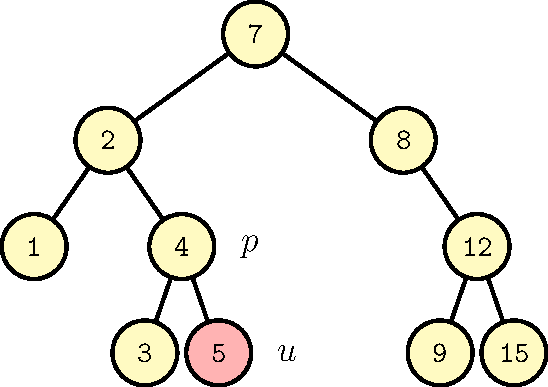
\includegraphics[width=\linewidth, page=1]{tree-abr-delete1}
			\caption{Individuazione nodo foglia}
		\end{subfigure}
		\hfill
		\begin{subfigure}[t]{.3\linewidth}
			\includegraphics[width=\linewidth, page=2]{tree-abr-delete1}
			\caption{Rimozione del nodo foglia}
		\end{subfigure}
		\hfill\null
	\end{figure}
	% NOTE aggiustamenti per fare rientrare tutto in una pagina
	\vspace{-15pt}
	\item se il nodo da eliminare ha un solo figlio \(f\) (destro o sinistro): si elimina \(u\) e si collega \(f\) all'ex-padre \(p\) di \(u\) in sostituzione di \(u\) (tramite la funzione \shortcut);
	le proprietà di ordinamento non vengono alterate in quanto tutti i nodi del sottoalbero destro di \(p\) sono maggiori di \(p\) stesso;
	% NOTE aggiustamenti per fare rientrare tutto in una pagina
	\vspace{-5pt}
	\begin{figure}[H]
		\begin{subfigure}[t]{.3\linewidth}
			\includegraphics[width=\linewidth, page=3]{tree-abr-delete1}
			\caption{Individuazione nodo \(u\) da eliminare}
		\end{subfigure}
		\hfill
		\begin{subfigure}[t]{.3\linewidth}
			\includegraphics[width=\linewidth, page=4]{tree-abr-delete1}
			\caption{Rimozione nodo \(u\)}
		\end{subfigure}
		\hfill
		\begin{subfigure}[t]{.3\linewidth}
			\includegraphics[width=\linewidth, page=5]{tree-abr-delete1}
			\caption{Collegamento del sottoalbero \(f\) di \(u\) al padre \(p\) di \(u\)}
		\end{subfigure}
	\end{figure}
	% NOTE aggiustamenti per fare rientrare tutto in una pagina
	\vspace{-15pt}
	\item se il nodo da eliminare \(u\) ha due figli: cerchiamo di ricadere nel caso {\footnotesize\ttfamily (2)};
	\begin{enumerate*}
		\item individuiamo il successore (predecessore) \(s\) di \(u\), il quale è il più piccolo valore maggiore di \(u\) (il più grande valore minore di \(u\)) e di conseguenza non ha figli sinistri (non ha figli destri);
		\item si \enquote{stacca} il successore \(s\);
		\item si collega l'eventuale figlio destro di \(s\) al padre (tramite la funzione \shortcut) in quanto trovandosi nel sottoalbero sinistro del nonno vuol dire che sicuramente il suo valore non è maggiore del padre di \(s\);
		\item si copia \(s\) su \(u\), si rimuove il nodo \(s\), così facendo rispetto comunque l'ordine parziale.
	\end{enumerate*}
	% NOTE aggiustamenti per fare rientrare tutto in una pagina
	\vspace{-5pt}
	\begin{figure}[H]
		\hfill
		\begin{subfigure}[t]{.45\linewidth}
			\includegraphics[width=\linewidth, page=2]{tree-abr-delete2}
			\caption{Individuiamo il successore \(s\) di \(u\)}
		\end{subfigure}
		\hfill
		\begin{subfigure}[t]{.45\linewidth}
			\includegraphics[width=\linewidth, page=3]{tree-abr-delete2}
			\caption{Si \enquote{stacca} il successore \(s\)}
		\end{subfigure}
		\hfill\null

		\vspace{10pt}

		\hfill
		\begin{subfigure}[t]{.45\linewidth}
			\includegraphics[width=\linewidth, page=4]{tree-abr-delete2}
			\caption{Si collega l'eventuale figlio destro di \(s\) al padre}
		\end{subfigure}
		\hfill
		\begin{subfigure}[t]{.45\linewidth}
			\includegraphics[width=\linewidth, page=5]{tree-abr-delete2}
			\caption{Si copia \(s\) su \(u\), si rimuove il nodo \(s\)}
		\end{subfigure}
		\hfill\null

		% NOTE rimosso perché la spiegazione risulta ugualmente chiara, e non ci starebbe tutto in una pagina diciamocelo
		% \vspace{10pt}
		%
		% \hfill
		% \begin{subfigure}[t]{.45\linewidth}
		% 	\includegraphics[width=\linewidth, page=5]{tree-abr-delete2}
		% 	\caption{bla bla bla}
		% \end{subfigure}
		% \hfill\null
	\end{figure}
\end{enumerate}

\clearpage
\subsection*{Costo computazionale delle operazioni}

Tutte le operazioni sono confinate ai nodi posizionati lungo un cammino semplice dalla radice ad una foglia.
Quindi se l'altezza dell'albero è definita come \(h\), il tempo di ricerca ha complessità \(\Omicron(h)\).

Il caso pessimo è rappresentanto da un albero sbilanciato completamente a destra o completamente a sinistra.
Questo caso può accadere quando si inseriscono ordinatamente i dati nell'albero.
Questo caso, dove l'altezza \(h = n\) porta ad una complessità \(\Omicron(n)\).

Mentre il caso ottimo è rappresentanto da un albero perfettamente bilanciato.
Nell'esempio è mostrato un albero perfetto con \(2^h - 1\) nodi, dove \(h\) è l'altezza.
In questo caso la complessità è pari a \(\Omicron(\log n)\), ad esempio con \(h = 2^3 - 1\) la complessità è \(\Omicron(\log h) = \Omicron(\log 7) < 3\).

Ci domandiamo quindi quale sia l'altezza media di un albero binario di ricerca.
Il caso \enquote{semplice} è quello di considerare che gli inserimenti avvengano in maniera statisticamente uniforme, è possibile dimostrare che l'altezza media è \(\Omicron(\log n)\), mentre il caso generale, ossia quello in cui avvengono sia inserimenti che cancellazioni è di difficile trattazione. Per evitare questa casistica si utilizzano varie tecniche per mantenere l'albero bilanciato.
Per capire queste tecniche abbiamo prima bisogno di fissare un concetto.
\begin{definition}[Fattore di bilanciamento]
Il fattore di bilanciamento \(\beta(v)\) di un nodo \(v\) è la massima differenza di altezza fra i sottoalberi di \(v\).
\end{definition}

Negli anni sono state usate diverse tecniche, ora in disuso:
\begin{itemize}
	\item Alberi AVL (1962): \(\beta(v) \leqslant 1\) per ogni nodo \(v\), il bilanciamento dell'albero avveniva tramite rotazioni;
	\item B-Alberi (1972): \(\beta(v) = 0\) per ogni nodo \(v\), sono specializzati per strutture in memoria secondaria;
	\item Alberi 2-3 (1983): \(\beta(v) = 0\) per ogni nodo \(v\), in cui ogni nodo può avere o 2 o 3 figli, se ad un nodo viene aggiunto un ulteriore figlio, il ramo viene spezzato in due rami con 2 figli ciascuno, mentre se ad un ramo con 2 figli ne viene tolto uno allora l'unico figlio rimanente viene collegato al padre, questo potrebbe riportare il problema al primo caso; il bilanciamento viene ottenuto quindi tramite merge/split, il grado è variabile.
\end{itemize}

\begin{note}[Meccanismo di rotazione]
Il meccanismo di rotazione ci permette di abbassare il fattore di sbilanciamento rispettando le proprietà di ordinamento parziale.
\end{note}

\clearpage
\section{Alberi Binari di Ricerca bilanciati}

\begin{definition}[Albero Red-Black]
Un albero red-black è un albero binario di ricerca in cui:
\begin{itemize}
	\item ogni nodo è colorato di rosso o di nero;
	\item le chiavi vengono mantenute solo nei nodi interni dell'albero;
	\item le foglie sono costituite solo da nodi speciali \textbf{Nil}.
\end{itemize}
\end{definition}

I nodi speciali \textbf{Nil} sono dei nodi sentinella il cui unico scopo è quello di evitare di trattare diversamente i puntatori ai nodi, dai puntatori \Nil;
infatti al posto di un puntatore \Nil si usa un puntatore ad un nodo \textbf{Nil};
in memoria ne esiste solo uno per motivi di economia.
I nodi con figli \textbf{Nil} sono le foglie nell'albero binario di ricerca corrispondente.

Un albero red-black deve rispettare i seguenti vincoli:
\begin{enumerate}
	\item la radice è nera;
	\item tutte le foglie sono nere;
	\item entrambi i figli di un nodo rosso sono neri;
	\item ogni cammino semplice da un nodo \(u\) ad una delle foglie contenute nel sottoalbero radicato in \(u\) ha lo stesso numero di nodi neri.
\end{enumerate}

\begin{algorithm}[H]
	\caption{Specifica \textsc{Red-Black Tree}}
	%&../preamble

% arara: pdflatex: { synctex: no }
% arara: latexmk: { clean: partial }
\ifstandalone
\begin{document}
\begin{algorithm}[H]
\fi

\BlankLine
\tcp{CONTENUTO DI UN NODO}

\BlankLine
\Tree \varParent\;
\Tree \varLeft\;
\Tree \varRight\;
\Int \alert{\varColor} \Comment*[l]{\RED o \BLACK}
\Item \varKey\;
\Item \varValue\;

\BlankLine
\tcp{GETTERS}

\BlankLine
\Tree \treeParent\;
\Tree \treeLeft\;
\Tree \treeRight\;
\Int \treeColor\;
\Item \treeKey\;
\Item \treeValue\;

\ifstandalone
\end{algorithm}
\end{document}
\fi

\end{algorithm}

\begin{property*}[Altezza nera di un nodo \(v\)]
L'altezza nera \(b(v)\) di un nodo \(v\) è il numero di nodi neri lungo ogni percorso da \(v\) (escluso) ad ogni foglia (inclusa) del suo sottoalbero.
\end{property*}

\begin{property*}[Altezza nera di un albero Red-Black]
L'altezza nera di un albero Red-Black è pari all'altezza nera della sua radice.
\end{property*}

Entrambe le proprietà sono ben definite perché tutti i percorsi hanno lo stesso numero di nodi neri (per via della regola no.\ 4).

\clearpage
\subsection*{Esempi}

Nelle suguenti figure i nodi neri sono segnati in bianco, mentre quelli rossi sono segnati.

\begin{figure}[H]\centering
	\renewcommand{\subfigurename}{Es.}
	\renewcommand\thesubfigure{\arabic{subfigure}}
	\captionsetup[subfigure]{labelformat=simple, labelsep=space}
	\begin{subfigure}[t]{.48\linewidth}\centering
		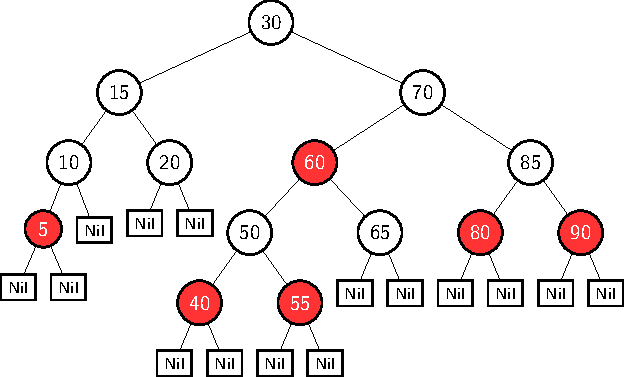
\includegraphics[width=\linewidth, page=1]{tree-rb-examples}
		\caption{Entrambi i figli di un nodo rosso sono neri (3),\\ma un nodo nero può avere figli neri.}
	\end{subfigure}
	\hfill
	\begin{subfigure}[t]{.48\linewidth}\centering
		\includegraphics[width=\linewidth, page=2]{tree-rb-examples}
		\caption{Ogni percorso da un nodo interno ad un nodo \textbf{Nil} ha lo stesso numero  di nodi neri (4).\\L'altezza nera di quest'albero è 3}
		\vspace{5pt}
	\end{subfigure}

	\begin{lemma}
	L'altezza totale di un albero è al più il doppio della sua altezza nera.
	\end{lemma}

	\begin{subfigure}[t]{.48\linewidth}\centering
		\includegraphics[width=\linewidth, page=2]{tree-rb-examples}
		\caption{Più colorazioni sono possibili (versione 1).\\L'altezza di questo albero è 3}
	\end{subfigure}
	\hfill
	\begin{subfigure}[t]{.48\linewidth}\centering
		\includegraphics[width=\linewidth, page=3]{tree-rb-examples}
		\caption{Più colorazioni sono possibili (versione 2).\\L'altezza di questo albero è 3}
	\end{subfigure}

	\begin{subfigure}[t]{.48\linewidth}\centering
		\includegraphics[width=\linewidth, page=4]{tree-rb-examples}
		\caption{Cambiare colorazione può cambiare l'altezza nera.\\L'altezza di questo albero è 3}
	\end{subfigure}
	\hfill
	\begin{subfigure}[t]{.48\linewidth}\centering
		\includegraphics[width=\linewidth, page=5]{tree-rb-examples}
		\caption{Cambiare colorazione può cambiare l'altezza nera.\\Stesso albero, l'altezza nera di questo albero è 2}
	\end{subfigure}
\end{figure}

% \clearpage
% \subsection*{Esercizio}
%
% \begin{figure}[ht]
% 	\caption*{Quasto albero può essere un albero Red-Black?}
% 	\vspace{5pt}
% 	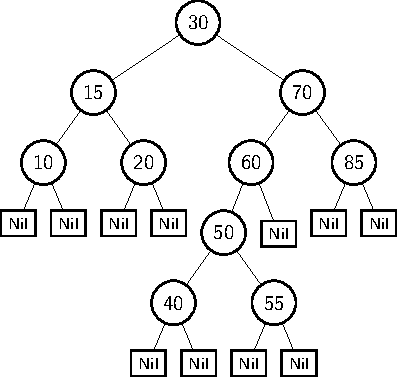
\includegraphics[width=\linewidth, height=4.5cm, keepaspectratio]{tree-rb-question}
% \end{figure}
% \vfill\null
% \clearpage

\clearpage
\subsection{Inserimento di un nodo}

Durante la modifica di un albero Red-Black è possibile che le condizioni di bilanciamento risultino violate.
Quando i vincoli Red-Black vengono violati si può agire in due modi:
\begin{itemize}
	\item modificando i colori nella zona della violazione;
	\item operando dei bilanciamenti dell'albero tramite rotazioni (a destra o a sinistra)
\end{itemize}

\subsection{Bilanciamento dell'albero}

\subsection*{Rotazione a sinistra}

\begin{algorithm}[H]
	% \caption{Rotazione di un \textsc{Red-Black Tree} a sinistra}
	\caption{Bilanciamento dell'albero tramite rotazione a sinistra}
	\setcounter{AlgoLine}{0}
	%&../preamble

% arara: pdflatex: { synctex: no }
% arara: latexmk: { clean: partial }
\ifstandalone
\begin{document}
\begin{algorithm}[H]
\fi

\BlankLine
\tcp{effettua una rotazione verso sinistra}
\prototype{\Tree \leftRotation{\Tree x}}{
	\lnl{case:primo-step}%
	\Tree \(y \Assign x.\treeRight\)\;
	\Tree \(p \Assign x.\treeParent\)\;

	\BlankLine
	\lnl{case:secondo-step}%
	\(x.\treeRight \Assign y.\treeLeft\) \Comment*[l]{il sottoalbero \(B\) diventa figlio destro di \(x\)}
	\If{\(y.\treeLeft \Neq \Nil\)}{
		\(y.\treeLeft.\treeParent \Assign x\)\;
	}

	\BlankLine
	\lnl{case:terzo-step}%
	\(y.\treeLeft \Assign x\) \Comment*[l]{\(x\) diventa figlio sinistro di \(y\)}
	\(x.\treeParent \Assign y\)\;

	\BlankLine
	\lnl{case:quarto-step}%
	\(y.\treeParent \Assign p\) \Comment*[l]{\(y\) diventa figlio di \(p\)}
	\If{\(p \Neq \Nil\)}{
		\eIf{\(p.\treeLeft \Equal x\)}{
			\(p.\treeLeft \Assign y\)
		}{
			\(p.\treeRight \Assign y\)
		}
	}

	\BlankLine
	\Return \(y\)\;
}

\ifstandalone
\end{algorithm}
\end{document}
\fi

\end{algorithm}

\begin{note}
Il disegno differisce minimamente da quello che si trova sulle slide per motivi di comodità nel disegnarli con \LaTeX{}
\end{note}
\begin{figure}[H]
	\renewcommand\thesubfigure{\arabic{subfigure}}
	\begin{subfigure}[t]{.23\linewidth}
		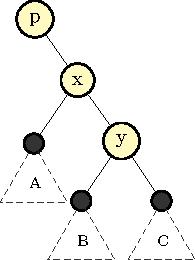
\includegraphics[width=\linewidth, page=1]{tree-rb-leftRotation}
		\caption{Stato iniziale}
	\end{subfigure}\hfill
	\begin{subfigure}[t]{.23\linewidth}
		\includegraphics[width=\linewidth, page=2]{tree-rb-leftRotation}
		\caption{Il sottoalbero \(B\) diventa figlio dx di \(x\)}
	\end{subfigure}\hfill
	\begin{subfigure}[t]{.23\linewidth}
		\includegraphics[width=\linewidth, page=3]{tree-rb-leftRotation}
		\caption{\(x\) diventa figlio sx di \(y\)}
	\end{subfigure}\hfill
	\begin{subfigure}[t]{.23\linewidth}
		\includegraphics[width=\linewidth, page=4]{tree-rb-leftRotation}
		\caption{\(y\) diventa figlio di \(p\),\\il vecchio padre di \(x\)}
	\end{subfigure}
	\caption{Esempio di rotazione a sinistra}
\end{figure}
\clearpage
\subsection*{Rotazione a destra}

La rotazione a destra è simmetrica e viene spiegata ed illustrata per completezza.

\begin{algorithm}[H]
	% \caption{Rotazione di un \textsc{Red-Black Tree} a destra}
	\caption{Bilanciamento dell'albero tramite rotazione a destra}
	\setcounter{AlgoLine}{0}
	%&../preamble

% arara: pdflatex: { synctex: no }
% arara: latexmk: { clean: partial }
\ifstandalone
\begin{document}
\begin{algorithm}[H]
\fi

\BlankLine
\tcp{effettua una rotazione verso destra}
\prototype{\Tree \rightRotation{\Tree x}}{
	\tcp{entrambi potrebbero essere \Nil}
	\lnl{case:primo-step}%
	\Tree \(y \Assign x.\treeLeft\)\;
	\Tree \(p \Assign x.\treeParent\)\;

	\BlankLine
	\lnl{case:secondo-step}%
	\(x.\treeLeft \Assign y.\treeRight\) \Comment*[l]{il sottoalbero \(B\) diventa figlio sinistro di \(x\)}
	\If{\(y.\treeRight \Neq \Nil\)}{
		\(y.\treeRight.\treeParent \Assign x\)\;
	}

	\BlankLine
	\lnl{case:terzo-step}%
	\(y.\treeRight \Assign x\) \Comment*[l]{\(x\) diventa figlio destro di \(y\)}
	\(x.\treeParent \Assign y\)\;

	\BlankLine
	\lnl{case:quarto-step}%
	\(y.\treeParent \Assign p\) \Comment*[l]{\(y\) diventa figlio di \(p\)}
	\If{\(p \Neq \Nil\)}{
		\If{\(p.\treeRight \Equal x\)}{
			\(p.\treeRight \Assign y\)
		}{
			\(p.\treeLeft \Assign y\)
		}
	}

	\BlankLine
	\Return \(y\)\;
}

\ifstandalone
\end{algorithm}
\end{document}
\fi

\end{algorithm}

\begin{figure}[H]
	\renewcommand\thesubfigure{\arabic{subfigure}}
	\begin{subfigure}[t]{.23\linewidth}
		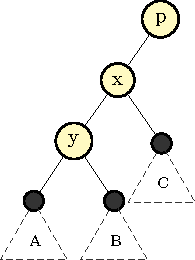
\includegraphics[width=\linewidth, page=1]{tree-rb-rightRotation}
		\caption{Stato iniziale}
	\end{subfigure}\hfill
	\begin{subfigure}[t]{.23\linewidth}
		\includegraphics[width=\linewidth, page=2]{tree-rb-rightRotation}
		\caption{Il sottoalbero \(B\) diventa figlio sx di \(x\)}
	\end{subfigure}\hfill
	\begin{subfigure}[t]{.23\linewidth}
		\includegraphics[width=\linewidth, page=3]{tree-rb-rightRotation}
		\caption{\(x\) diventa figlio dx di \(y\)}
	\end{subfigure}\hfill
	\begin{subfigure}[t]{.23\linewidth}
		\includegraphics[width=\linewidth, page=4]{tree-rb-rightRotation}
		\caption{\(y\) diventa figlio di \(p\),\\il vecchio padre di \(x\)}
	\end{subfigure}
	\caption{Esempio di rotazione a destra}
\end{figure}

\clearpage
\subsection*{Inserimento di un nodo in un albero binario bilanciato}

Per inserire un nodo in un albero Red-Black si usa la stessa procedura usata per gli alberi binari di ricerca e si colora il nuovo nodo di \RED.
Il vincolo che potremmo violare è il terzo, quello che prevede che entrambi i figli di un nodo rosso siano neri.

\begin{algorithm}[H]
	\caption{Inserimento di un nodo in un \textsc{Red-Black Tree}}
	%&../preamble

% arara: pdflatex: { synctex: no }
% arara: latexmk: { clean: partial }
\ifstandalone
\begin{document}
\begin{algorithm}[H]
\fi

\BlankLine
\tcp{Inserimento di un nodo in un albero Red-Black}
\prototype{\Tree \insertNode{\Tree T, \Tree k, \Item x}}{
	\Tree \(p \Assign \Nil\) \Comment*[l]{riferimento al padre}
	\Tree \(u \Assign T\) \Comment*[l]{riferimento alla radice}

	\BlankLine
	\tcp{cerco posizione inserimento}
	\While{\(u \Neq \Nil\) \And \(u.\treeKey \Neq k\)}{
		\(p \Assign u\)\;
		\(u\) \Assign \iif{\(k < u.\treeKey, u.\treeLeft, u.\treeRight\)}\;
	}

	\BlankLine
	\eIf{\(u \Neq \Nil\) \And \(u.\treeKey \Equal k\)}{
		\tcp{la chiave è già presente, aggiorno il valore}

		\BlankLine
		\(u.\treeValue \Assign v\)\;
	}{
		\tcp{la chiave non è presente}
		\tcp{creo un nodo coppia chiave-valore}
		\Tree \(new\) \Assign \treeConstructor{\(k, v\)}\;

		\BlankLine
		\tcp{collego il nodo creato}
		\shortcut{\(p, new, k\)}\;

		\alert{\treeFixInsert{\(new\)}}\;

		\BlankLine
		\If{\(p \Equal \Nil\)}{
			\(T \Assign new\) \Comment*[l]{primo nodo ad essere inserito}
		}
	}

	\BlankLine
	\tcp{restituisco l'albero non modificato o il nuovo nodo}
	\Return \(T\)\;
}

\ifstandalone
\end{algorithm}
\end{document}
\fi

\end{algorithm}

Nel caso in cui l'inserimento vìoli il terzo vincolo ci sposteremo verso l'alto lungo il percorso di inserimento;
cercheremo di ripristinare il terzo vincolo;
sposteremo le violazioni verso l'alto rispettando il quarto vincolo (mantenendo l'altezza nera dell'albero);
al termine, coloreremo la radice di nero (onorando il primo vincolo).

\begin{note}
Le operazioni di ripristino sono necessarie solo quando due nodi consecutivi sono rossi, altrimenti non sono necessarie.
\end{note}

\clearpage
\begin{algorithm}[H]
	\caption{Bilanciamento dell'albero in seguito all'inserimento di un nodo rosso}
	\setcounter{AlgoLine}{0}
	%&../preamble

% arara: pdflatex: { synctex: no }
% arara: latexmk: { clean: partial }
\ifstandalone
\begin{document}
\begin{algorithm}[H]
\fi

\BlankLine
% \tcp{bilanciamento di un \textsc{Red-Black Tree} in seguito all'inserimento di un nodo \RED}
\prototype{\treeFixInsert{\Tree t}}{

	\BlankLine
	\(t.\treeColor \Assign \RED\) \Comment*[l]{coloro il nodo da inserire di rosso}

	\BlankLine
	\tcp{\(t \Equal \Nil\) è la condizione di fino ciclo}
	\While{\(t \Neq \Nil\)}{

		\BlankLine
		\lnlset{case:refences}{0}%
		\Tree \(p \Assign t.\treeParent\) \Comment*[r]{riferimento al padre}
		\Tree \(n \Assign\) \iif{\(p \Neq \Nil, p.\treeParent, \Nil\)} \Comment*[r]{riferimento al nonno}
		\Tree \(z \Assign\) \iif{\(n \Equal \Nil, \Nil\), \iif{\(n.\treeLeft \Equal p, n.\treeRight, n.\treeLeft\)}} \Comment*[r]{riferimento allo zio}

		\BlankLine
		\lnl{case:no-father}%
		\uIf{\(p \Equal \Nil\)}{
			\(t.\treeColor \Assign \BLACK\)\;
			\(t \Assign \Nil\) \Comment*[l]{fine}
			\BlankLine

		}%
		\lnl{case:black-father}
		\uElseIf{\(p.\treeColor \Equal \BLACK\)}{
			\(t \Assign \Nil\) \Comment*[l]{fine}
			\BlankLine

		}%
		\lnl{case:red-aunt}
		\uElseIf{\(z.\treeColor \Equal \RED\)}{
			\(p.\treeColor \Assign z.\treeColor \Assign \BLACK\)\;
			\(n.\treeColor \Assign \RED\)\;
			\(t \Assign n\) \Comment*[l]{passo il problema al nonno}
			\BlankLine

		}\Else{

			\BlankLine
			\lnlset{right-left}{4a}%
			\uIf{(\(t \Equal p.\treeRight\)) \And (\(p \Equal n.\treeLeft\))}{
				\leftRotation{\(p\)}\;
				\(t \Assign p\) \Comment*[l]{passo il problema al padre}
				\BlankLine

			}%
			\lnlset{left-right}{4b}%%
			\eIf{(\(t \Equal p.\treeLeft\)) \And (\(p \Equal n.\treeRight\))}{
				\rightRotation{\(p\)}\;
				\(t \Assign p\) \Comment*[l]{passo il problema al padre}
				\BlankLine

			}{%
				\BlankLine
				\lnlset{left-left}{5a}%
				\uIf{(\(t \Equal p.\treeLeft\)) \And (\(p \Equal n.\treeLeft\))}{
					\rightRotation{\(n\)}\;
				}%
				\lnlset{right-right}{5b}%
				\ElseIf{(\(t \Equal p.\treeRight\)) \And (\(p \Equal n.\treeRight\))}{
					\leftRotation{\(n\)}\;
				}

				\BlankLine
				\(p.\treeColor \Assign \BLACK\)\;
				\(n.\treeColor \Assign \RED\)\;
				\(t \Assign \Nil\) \Comment*[l]{fine}
			}
		}
	}
}

\ifstandalone
\end{algorithm}
\end{document}
\fi

\end{algorithm}

\clearpage
\begin{enumerate}[label={\footnotesize\ttfamily (\arabic*)}, start=0]

	\vspace{-5pt}
	\item dichiaro dei riferimento al padre, al nonno e allo zio
	\begin{figure}[H]\centering
		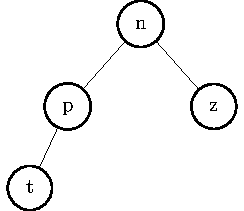
\includegraphics[page=1]{tree-rb-insertNode}
	\end{figure}

	\vspace{-5pt}
	\item il nuovo nodo \(t\) non ha padre; Questo può accadere in due casi:
		\begin{compactlist}
			\item è il primo nodo ad essere inserito, oppure
			\item quando abbiamo spostato la violazione verso l'alto fino a raggiungere la radice
		\end{compactlist}
	Ricoloriamo \(t\) di \BLACK in quanto trovandosi sulla radice dell'albero non viola nessun vincolo.

	\vspace{-5pt}
	\begin{figure}[H]\centering
		\begin{subfigure}[t]{.5\textwidth}\centering
			\includegraphics[width=.3\linewidth, page=2]{tree-rb-insertNode}
			\caption{Possibile violazione del primo vincolo}
		\end{subfigure}%
		\begin{subfigure}[t]{.5\textwidth}\centering
			\includegraphics[width=.3\linewidth, page=3]{tree-rb-insertNode}
			\caption{Ricolorazione del nodo \(t\)}
		\end{subfigure}
		% \caption{Spostamento del problema verso l'alto}
	\end{figure}

	\vspace{-5pt}
	\item il padre \(p\) di \(t\) è nero; anche in questo caso non abbiamo violato nessun vincolo perché avendo inserito un nodo rosso la lunghezza dei cammini neri non cambia e avendo inserito un nodo rosso figlio di un nodo nero non violiamo il terzo vincolo;

	\vspace{-5pt}
	\begin{figure}[H]\centering
		\includegraphics[page=4]{tree-rb-insertNode}
	\end{figure}

	\vspace{-5pt}
	\item il padre \(p\) e lo zio \(z\) sono rossi; Se \(z\) è rosso è possibile ricolorare di nero \(p\) e \(z\), e di rosso \(n\); poiché tutti i cammini che passano per \(z\) e \(p\) passano anche per \(n\), l'altezza nera non è cambiata (non abbiamo violato il quarto vincolo); Abbiamo spostato così il problema verso l'alto, più precisamente sul nonno che potrebbe aver violato il primo o il terzo vincolo, ovvero che \(n\) può essere una radice rossa o che abbia un padre rosso. Per risolvere il problema poniamo \(t \Assign n\) e continuiamo il ciclo.

	\vspace{-5pt}
	\begin{figure}[H]\centering
		\begin{subfigure}[t]{.5\textwidth}
			\includegraphics[width=\linewidth, page=5]{tree-rb-insertNode}
			\caption{Possibile violazione del primo e del terzo vincolo}
		\end{subfigure}%
		\begin{subfigure}[t]{.5\textwidth}
			\includegraphics[width=\linewidth, page=6]{tree-rb-insertNode}
			\caption{Ricolorazione del padre e dello zio di nero}
		\end{subfigure}
		% \caption{Spostamento del problema verso l'alto}
	\end{figure}

	\item[\footnotesize\ttfamily (4a)] il padre \(p\) è rosso e lo zio \(z\) è nero; si assuma che \(t\) sia figlio \emph{destro}  di \(p\) e che \(p\) sia figlio \emph{sinistro}  di \(n\); effettuando una rotazione a sinistra a partire dal nodo \(p\) scambiamo i ruoli di \(t\) e d \(p\) ottenendo il caso {\footnotesize\ttfamily (5a)}, dove i nodi in conflitto sul terzo vincolo sono entrambi figli \emph{sinistri} dei loro padri; i nodi coinvolti nel cambiamento sono \(p\) e \(t\), entrambi rossi, quindi l'altezza nera non cambia; abbiamo spostato il problema al padre, quindi poniamo \(t \Assign p\) e continuiamo il ciclo.

	\item[\footnotesize\ttfamily (4b)] speculare al caso {\footnotesize\ttfamily (4a)} (ossia che che \(t\) sia figlio \emph{sinistro}  di \(p\) e che \(p\) sia figlio \emph{destro}  di \(n\))

	\begin{figure}[H]\centering
		\begin{subfigure}[t]{.5\textwidth}
			\includegraphics[width=\linewidth, page=7]{tree-rb-insertNode}
			\caption{Possibile violazione del primo e del terzo vincolo}
		\end{subfigure}%
		\begin{subfigure}[t]{.5\textwidth}
			\includegraphics[width=\linewidth, page=8]{tree-rb-insertNode}
			\caption{Ricolorazione del padre e dello zio di nero}
		\end{subfigure}
		\caption[]{Rappresentazione grafica del caso {\footnotesize\ttfamily (4a)}}
	\end{figure}

	\item[\footnotesize\ttfamily (5a)] anche in questo caso il padre \(p\) è rosso e lo zio \(z\) è nero; ma si assuma che \(t\) sia figlio \emph{sinistro} di \(p\) e che \(p\) sia figlio \emph{sinistro}  di \(n\); effettuando una rotazione a destra a partire dal nodo \(n\) ci porta ad una situazione in cui \(t\) e \(n\) sono figli di \(p\); colorando \(p\) di nero ed \(n\) di rosso ci troviamo in una situazione in cui tutti i vincoli vengono rispettati (in particolare, l'altezza nera che passano per la radice è uguale a quella iniziale).

	\item[\footnotesize\ttfamily (5b)] speculare al caso {\footnotesize\ttfamily (5a)} (ossia che che che \(t\) sia figlio \emph{destro} di \(p\) e che \(p\) sia figlio \emph{destro}  di \(n\))

	\begin{figure}[H]\centering
		\begin{subfigure}[t]{.5\textwidth}
			\includegraphics[width=\linewidth, page=8]{tree-rb-insertNode}
			\caption{Possibile violazione del primo e del terzo vincolo}
		\end{subfigure}%
		\begin{subfigure}[t]{.5\textwidth}
			\includegraphics[width=\linewidth, page=9]{tree-rb-insertNode}
			\caption{Ricolorazione del padre e dello zio di nero}
		\end{subfigure}
		\caption[]{Rappresentazione grafica del caso {\footnotesize\ttfamily (5a)}}
	\end{figure}
\end{enumerate}

\paragraph{Complessità}
Ognuna di queste operazione avviene in tempo costante.
Ogni volta il problema può salire di uno o due livelli, in quanto l'altezza dell'albero è limitata da \(\log n\), il nostro algoritmo è limitato superiormente da \(\log n\), ossia \(\Omicron(\log n)\).

Più precisamente:
\begin{itemize}
	\item \(\Omicron(\log n)\) per scendere fino al punto di inserimento;
	\item \(\Omicron(1)\) per effettuare l'inserimento;
	\item \(\Omicron(\log n)\) per risalire ed \enquote{aggiustare} (caso {\footnotesize\ttfamily 3})
\end{itemize}

\clearpage
\subsection*{Esempi di inserimento}

Proviamo ad inserire il nodo \(16\) nell'albero red-black sottostante.

\begin{figure}[H]\centering
	% \renewcommand{\subfigurename}{Es.}
	% \renewcommand\thesubfigure{\arabic{subfigure}}
	% \captionsetup[subfigure]{labelformat=simple, labelsep=space}
	\begin{subfigure}[t]{.48\linewidth}\centering
		\includegraphics[width=\linewidth, page=1]{tree-rb-insertNode-example-1}
		\caption{Stato attuale}
	\end{subfigure}
	\hfill
	\begin{subfigure}[t]{.48\linewidth}\centering
		\includegraphics[width=\linewidth, page=2]{tree-rb-insertNode-example-1}
		\caption{Inserimento del nodo \(16\) andato a buon fine}
	\end{subfigure}
\end{figure}

\vspace{-5pt}
Non violiamo alcun vincolo in quanto il padre di \(16\) è nero e non abbiamo modificato l'altezza nera.
Questo caso rappresenta il caso {\footnotesize\ttfamily 2}, l'inserimento del nodo \(16\) è quindi andato a buon fine.
Alternativamente proviamo ad inserire il nodo \(42\) sempre nello stesso albero.

% \vspace{-5pt}
\begin{figure}[H]\centering
	\begin{subfigure}[t]{.48\linewidth}\centering
		\includegraphics[width=\linewidth, page=2]{tree-rb-insertNode-example-2}
		\caption{Inserimento del nodo \(42\), violiamo il secondo vincolo, ci troviamo nel caso {\footnotesize\ttfamily 3} (\(z\) rosso), quindi coloriamo di nero \(p\) e \(z\) e di rosso \(n\), il problema si sposta ad \(n\)}
	\end{subfigure}
	\hfill
	\begin{subfigure}[t]{.48\linewidth}\centering
		\includegraphics[width=\linewidth, page=3]{tree-rb-insertNode-example-2}
		\caption{Violiamo il terzo vincolo, entrambi i nodi rossi sono figli \emph{sinistri} quindi ci troviamo nel caso {\footnotesize\ttfamily 5a}, quindi coloriamo di nero \(p\), di rosso \(n\) \dots}
	\end{subfigure}

	\vspace{5pt}

	\begin{subfigure}[t]{.48\linewidth}\centering
		\includegraphics[width=\linewidth, page=4]{tree-rb-insertNode-example-2}
		\caption{\dots ed effettuiamo una rotazione a destra con perno \(n\)}
	\end{subfigure}
	\hfill
	\begin{subfigure}[b]{.48\linewidth}\centering
		\includegraphics[width=\linewidth, page=5]{tree-rb-insertNode-example-2}
		\caption{Abbiamo ripristinato il terzo vincolo, gli altri vincoli non sono mai stati violati, quindi abbiamo finito}
	\end{subfigure}
\end{figure}
\vspace{-10pt}

Questo esempio ci mostra chiaramente come gli alberi Red-Black, attraverso il rispetto dei vincoli, tendano a mantenere bilanciato l'albero.
Esiste una versione \emph{top-down} dell'algoritmo di inserimento che scende fino interessato \enquote{aggiustando} l'albero man mano.

\clearpage
\subsection{Rimozione di un nodo}

Se il nodo rimosso è rosso l'altezza nera rimane invariata, non sono stati creati nodi rossi consecutivi e la radice resta nera.
Il problema sorge quando si rimuovono nodi neri in quanto è possibile che siano stati violati il primo ed il terzo vincolo e sicuramente è stato violato il quarto vincolo in quanto cambia l'altezza nera.
L'algoritmo \treeFixDelete{\(T, t\)} ripristina la proprietà Red-Black con rotazioni e cambiamenti di colore.
Ci sono quattro casi possibili (e 4 simmetrici).
% A lezione non è stato spiegato l'algoritmo, viene riportato solo per completezza.

\vspace{-5pt}
\begin{algorithm}[H]
	\caption{Rimozione di un nodo in un \textsc{Red-Black Tree}}
	% \caption{Bilanciamento dell'albero in seguito alla rimozione di un nodo}
	% NOTE non presente nel documento finale
	% \input{tree-rb-removeNode}
	\setcounter{AlgoLine}{0}
	%&../preamble

% arara: pdflatex: { synctex: no }
% arara: latexmk: { clean: partial }
\ifstandalone
\begin{document}
\begin{algorithm}[H]
\fi

\BlankLine
% \tcp{bilanciamento di un \textsc{Red-Black Tree} in seguito alla rimozione di un nodo \RED}
\prototype{\treeFixDelete{\Tree T, \Tree t}}{

	\BlankLine
	\(t.\treeColor \Assign \RED\) \Comment*[l]{coloro il nodo da inserire di rosso}

	\BlankLine
	\While{(\(t \Neq T\)) \And (\(t.\treeColor \Equal \BLACK\))}{

		\BlankLine
		\Tree \(p \Assign t.\treeParent\) \Comment*[r]{riferimento al padre}

		\BlankLine
		\eIf{\(t \Equal p.\treeLeft\)}{

			\BlankLine
			\Tree \(f \Assign p.\treeRight\) \Comment*[r]{riferimento al fratello}
			\Tree \(ns \Assign f.\treeLeft\) \Comment*[r]{riferimento al nipote sinistro}
			\Tree \(nd \Assign f.\treeRight\) \Comment*[r]{riferimento al nipote destro}

			\BlankLine
			\lnl{caso1}%
			\eIf{\(f.\treeColor \Equal \RED\)}{
				\(p.\treeColor \Assign \RED\)\;
				\(f.\treeColor \Assign \BLACK\)\;
				\leftRotation{\(p\)}\;
				\tcp{t viene lasciato inalterato, quindi si ricade nei casi 2, 3, 4}
				\BlankLine

			}{

				\lnl{caso2}%
				\uIf{\(ns.\treeColor \Equal nd.\treeColor \Equal \BLACK\)}{
					\(f.\treeColor \Equal \RED\)\;
					\(t \Assign p\) \Comment*[l]{passo il problema al padre}
					\BlankLine

				}%
				\lnl{caso3}%
				\uElseIf{(\(ns.\treeColor \Equal \RED\)) \And (\(nd.\treeColor \Equal \BLACK\))}{
					\(ns.\treeColor \Assign \BLACK\)\;
					\(f.\treeColor \Assign  \RED\)\;
					\rightRotation{\(f\)}\;
					\tcp{t viene lasciato inalterato, quindi si ricade nel caso 4}
					\BlankLine

				}%
				\lnl{caso4}%
				\ElseIf{\(nd.\treeColor \Equal \RED\)}{
					\(f.\treeColor \Equal p.\treeColor\)\;
					\(p.\treeColor \Assign \BLACK\)\;
					\(nd.\treeColor \Assign \BLACK\)\;
					\leftRotation{\(p\)}\;
					\(t \Assign T\)\;
				}
			}
		}{
			\tcp{casi speculari}
		}
	}
}

\ifstandalone
\end{algorithm}
\end{document}
\fi

\end{algorithm}
\vspace{-10pt}

La cancellazione è concettualmente complicata, ma è efficiente.
\begin{enumerate}[label={\footnotesize\ttfamily (\arabic*)}, noitemsep, topsep = 5pt, parsep = 5pt, partopsep = 0pt]
	\item si passa ad uno dei casi 2, 3, 4;
	\item si torna ad uno degli altri casi, ma risalendo di un livello l'albero;
	\item si passa al caso 4;
	\item si termina.
\end{enumerate}

% \paragraph{Complessità}
\`{E} possibile visitare al massimo un numero \(\Omicron(\log n)\) di casi, ognuno dei quali è gestito in \(\Omicron(1)\).

\ifsubfile
\end{document}
\fi

	%&../settings/preamble.main

\ifsubfile
\pagestyle{plain}
\setcounter{chapter}{6}

% arara: pdflatex: { options: ["--output-directory=../build/chapters"], draft: yes, synctex: no }
% arara: pdflatex: { options: ["--output-directory=../build/chapters"], synctex: no }
\begin{document}
\fi
\chapter{Hashing}

\ifsubfile
\end{document}
\fi

	%&../settings/preamble.main

\ifsubfile
\pagestyle{plain}
\setcounter{chapter}{7}

% arara: pdflatex: { options: ["--output-directory=../build"], draft: yes, synctex: no }
% arara: pdflatex: { options: ["--output-directory=../build"], synctex: no }
\begin{document}
\fi
\chapter{Insiemi}

Possono essere implementati con molte delle strutture dati viste fin'ora.
Ognuna delle quali rappresenta valntaggi e svantaggi.

\section{Realizzazione con vettori booleani}

L'insieme viene rappresentato attraverso un vettore booleano di \(m\) elementi.
Il quale è notevolmente semplice da implementare ed estremamente efficiente verificare se un elemento appartiene all'insieme.
Sfortunatamente la memoria occupata è \(\Omicron(m)\), indipendentemente dalle dimensioni effettive, inoltre alcune operazioni dipendono dalla memoria utilizzata per memorizzare questi oggetti, piuttosto che dal numero di oggetti effettivamente memorizzati, il che porta ad una complessità di queste operazione di \(\Omicron(m)\).

\begin{algorithm}[H]
	\caption[Struttura dati insieme implementata come Vettore Booleano]
	        {Struttura dati \textsc{Set} implementata come Vettore Booleano}
	%&../preamble

% arara: pdflatex: { synctex: no }
% arara: latexmk: { clean: partial }
\ifstandalone
\begin{document}
\begin{algorithm}[H]
% \caption{Struttura dati \textsc{Set} implementata come Vettore Booleano}
% \the\columnsep
% \setlength{\columnsep}{-3.5cm}
% \the\columnsep
% \begin{multicols}{2}
\fi
% Una struttura dati \emph{dinamica}, \emph{non lineare} che memorizza una \emph{collezione non ordinata di elementi} senza valori ripetuti.

\begin{minipage}[t]{.4\textwidth}
\BlankLine
\Array{\Bool} \(V\)\;
\Int \(size\)\;
\Int \(dim\)\;

\BlankLine
\prototype{\Set \setConstructor{\Int m}}{
	\Set \(t \Assign\) \new \Set\;
	\(t.\varSize \Assign 0\)\;
	\(t.\varCapacity \Assign m\)\;
	\(t.V \Assign [\False] * m\)\;

	\BlankLine
	\Return \(t\)\;
}

\BlankLine
\prototype{\Set \setContains{\Int \(x\)}}{

	\BlankLine
	\eIf{\(1 \leqslant x \leqslant \varCapacity\)}{
		\Return \(V[x]\)\;
	}{
		\Return \(\False\)\;
	}
}

\BlankLine
\prototype{\Int \setSize}{
	\Return \(\varSize\)\;
}

\BlankLine
\prototype{\setInsert{\Int \(x\)}}{
	\If{\(1 \leqslant x \leqslant \varCapacity\)}{
		\If{\Not \(V[x]\)}{
			\(\Increment{\varSize}\)\;
			\(V[x] \Assign \True\)\;
		}
	}
}

\BlankLine
\prototype{\setRemove{\Int \(x\)}}{
	\If{\(1 \leqslant x \leqslant \varCapacity\)}{
		\If{\(V[x]\)}{
			\(\Decrement{\varSize}\)\;
			\(V[x] \Assign \False\)\;
		}
	}
}

\end{minipage}%
\begin{minipage}[t]{.5\textwidth}

\BlankLine
\prototype{\Set \setUnion{\Set \(A\), \Set \(B\)}}{
	\tcp{crea un insieme della capacità max}
	\Set \(C \Assign\) \setConstructor{\maxFunction{\(A.\varCapacity, A.\varCapacity\)}}\;

	\BlankLine
	\tcp{inserisci gli elementi di \(A\)}
	\From{\(i \Assign 1\) \DownTo \(A.\varCapacity\)}{
		\If{\(A.\setContains{i}\)}{
			\(C.\setInsert{i}\)\;
		}
	}

	\BlankLine
	\tcp{inserisci gli elementi di \(B\)}
	\From{\(i \Assign 1\) \DownTo \(B.\varCapacity\)}{
		\If{\(A.\setContains{i}\)}{
			\(C.\setInsert{i}\)\;
		}
	}
}

\BlankLine
\prototype{\Set \setIntersection{\Set \(A\), \Set \(B\)}}{
	\tcp{crea un insieme della capacità min}
	\Set \(C \Assign\) \setConstructor{\(\minFunction{A.\varCapacity, A.\varCapacity}\)}\;

	\BlankLine
	\From{\(i \Assign 1\) \DownTo \(\minFunction{A.\varCapacity, A.\varCapacity}\)}{
		\tcp{se è contenuto in entambi}
		\If{\(A.\setContains{i}\) \And \(B.\setContains{i}\)}{
			\(C.\setInsert{i}\) \Comment*[l]{aggiungilo}
		}
	}
}

\BlankLine
\prototype{\Set \setDifference{\Set \(A\), \Set \(B\)}}{
	\Set \(C \Assign\) \setConstructor{\(A.\varCapacity\)}\;

	\BlankLine
	\From{\(i \Assign 1\) \DownTo \(A.\varCapacity\)}{
		\tcp{se è contenuto \(A\) e non in \(B\)}
		\If{\(A.\setContains{i}\) \And \Not \(B.\setContains{i}\)}{
			\(C.\setInsert{i}\) \Comment*[l]{aggiungilo}
		}
	}
}

% \vspace{35pt}
% \vphantom{0pt}

\end{minipage}
\ifstandalone
% \end{multicols}
% \the\columnsep
% \setlength{\columnsep}{10pt}
% \the\columnsep
\end{algorithm}
\end{document}
\fi

\end{algorithm}

\clearpage
\subsection{Implementazioni nei linguaggi di programmazione}

Esistono alcune implementazioni nei linguaggi attualmente utilizzati.
In Java esiste la struttura dati \texttt{BitSet} i cui meotodi sono illustrati nella tabella~\ref{tab:java-set-implementation}.
Mentre in \texttt{C++ STL} esistono due implementazioni \texttt{std::bitset} e \texttt{vector<bool>}:
\begin{itemize}
	\item \texttt{bitset} è una struttura dati con dimensione fissata nel template al momento della compilazione;
	\item \texttt{vector<bool>} è una specializzazione di \texttt{vector} per ottimizzare la memorizzazione, ha dimensione dinamica.
\end{itemize}

\begin{table}[ht]
	\centering
	\caption{Implementazione \texttt{java.util.BitSet}}%
	\label{tab:java-set-implementation}
	\begin{tabular}{@{} l >{\ttfamily}l @{}}
	\toprule
		Operazione & \normalfont{Metodo} \\
	\midrule
		\setContains & boolean get(int i) \\
		\setSize & int cardinality() \\
		\setInsert & void set(int i) \\
		\setRemove & void clear(int i) \\
		\setUnion & void and(BitSet set) \\
		\setIntersection & void or(BitSet set) \\
		% \setDifference & \\
	\bottomrule
	\end{tabular}
\end{table}

\vspace{-10pt}
\section{Realizzazione con vettore non ordinato}

\begin{algorithm}[H]
	\caption[Struttura dati insieme implementata come vettore non ordinato]
	        {Struttura dati \textsc{Set} implementata come vettore non ordinato}
	%&../preamble

% arara: pdflatex: { synctex: no }
% arara: latexmk: { clean: partial }
\ifstandalone
\begin{document}
\begin{algorithm}[H]
% \caption{Struttura dati \textsc{Set} implementata come vettore non ordinato}
\fi

\prototype{\Set \setDifference{\Set \(A\), \Set \(B\)}}{
	\Set \(C \Assign\) \setConstructor \Comment*[l]{non ha bisogno della dimensione}

	\BlankLine
	\From{\(s \in A\)}{
		\tcp{se non è contenuto in \(B\)}
		\If{\Not \(B.\setContains{s}\)}{
			\(C.\setInsert{s}\) \Comment*[l]{aggiungilo}
		}
	}
}

\ifstandalone
\end{algorithm}
\end{document}
\fi

\end{algorithm}

\paragraph{Costo delle operazioni}
Le operazioni di ricerca, inserimento e cancellazione costano \(\Omicron(n)\), le operazioni di inserimento (assumendo che non esista l'elemento) costano \(\Omicron(1)\), le operazioni di unione, intersezione e differenza \(\Omicron(nm)\).

\clearpage
\section{Realizzazione vettore ordinato}

\begin{algorithm}[H]
	\caption*{Struttura dati \textsc{Set} implementata come vettore ordinato}
	%&../preamble

% arara: pdflatex: { synctex: no }
% arara: latexmk: { clean: partial }
\ifstandalone
\begin{document}
\begin{algorithm}[H]
% \caption{Struttura dati \textsc{Set} implementata come vettore ordinato}
\fi

\prototype{\Set \setIntersection{\List \(A\), \List \(B\)}}{

	\BlankLine
	\List \(C\) \Assign \setConstructor \Comment*[l]{non ha bisogno della dimensione}

	\tcp{creo puntatori alle liste}
	\Pos \(p\) \Assign \(A\).\listHead\;
	\Pos \(q\) \Assign \(B\).\listHead\;

	\BlankLine
	\While{\Not \(A.\listEnd{p}\) \And \(B.\listEnd{q}\)}{

		\BlankLine
		\uIf(\tcp*[h]{se gli elementi coincidono}){\(A.\listRead{p} \Equal B.\listRead{q}\)}{
			\(C\).\listInsert{\(C\).\listTail, \(A\).\listRead{\(p\)}} \Comment*[l]{inseriscilo nell'intersezione}
			\tcp{scorri i puntatori}
			\(p\) \Assign \(A\).\listSucc{\(p\)}\;
			\(q\) \Assign \(B\).\listSucc{\(q\)}\;
		}
		\uElseIf{\(A.\listRead{p} < B.\listRead{q}\)}{
			\(p\) \Assign \(A\).\listSucc{\(p\)} \Comment*[l]{scorro puntatore di \(A\)}
		}
		\Else{
			\(q\) \Assign \(B\).\listSucc{\(q\)} \Comment*[l]{scorro puntatore di \(B\)}
		}
	}
}

\ifstandalone
\end{algorithm}
\end{document}
\fi

\end{algorithm}

\paragraph{Costo delle operazioni}
Le operazioni di ricerca costano \(\Omicron(n)\) con le liste e \(\Omicron(\log n)\) con i vettori, le operazioni di inserimento e cancellazione costano \(\Omicron(n)\), le operazioni di unione, intersezione e differenza \(\Omicron(n)\).

\section{Reality Check}

In realtà si utilizzano strutture dati complesse che permettono di ottimizzare le performance.
Se abbiamo bisogno dell'ordinamento si utilizzano alberi bilanciati, mentre se abbiamo bisogno di sapere smeplicemente se un elemento è contenuto o meno si utilizzano le tabelle hash.

\medskip
Per le operazioni di ricerca, inserimento e cancellazione negli alberi bilanciati hanno una complessità di \(\Omicron(\log n)\), mentre nelle tabelle hash di \(\Omicron(1)\).

\medskip
Le implementazioni più diffuse degli alberi bilanciati sono \texttt{TreeSet} in Java, \texttt{OrderedSet} in Python e \texttt{set} in \texttt{C++}, mentre le implementazioni più diffuse delle tabelle hash sono \texttt{HashSet} in Java, \texttt{set} in Python e \texttt{unordered\_set} in \texttt{C++}.

\begin{table}[!ht]
	\centering
	\caption[Implementazioni e relative complessità delle operazioni sugli insiemi]{Implementazioni e relative complessità delle operazioni\\\(m \equiv\) dimensione del vettore o della tabella hash}%
	\label{tab:set-resume}
	\begin{tabular}{@{} *8{l} @{}}
	\toprule
		& \makecell[l]{\setContains\\\lookup} & \setInsert & \setRemove & \makecell[l]{\minFunction\\\maxFunction} & \makecell[l]{\textsf{foreach}\\(memoria)} & Ordine \\
	\cmidrule{2-7}
		Vettore booleano & \(\Omicron(1)\) & \(\Omicron(1)\) & \(\Omicron(1)\) & \(\Omicron(m)\) & \(\Omicron(m)\) & Sì\\
	\addlinespace
		Lista non ordinata & \(\Omicron(n)\) & \(\Omicron(n)\) & \(\Omicron(n)\) & \(\Omicron(n)\) & \(\Omicron(n)\) & No\\
	\addlinespace
		Lista ordinata & \(\Omicron(n)\) & \(\Omicron(n)\) & \(\Omicron(n)\) & \(\Omicron(1)\) & \(\Omicron(n)\) & Sì\\
	\addlinespace
		Vettore ordinato & \(\Omicron(\log n)\) & \(\Omicron(n)\) & \(\Omicron(n)\) & \(\Omicron(1)\) & \(\Omicron(n)\) & Sì\\
	\addlinespace
		Alberi bilanciati & \(\Omicron(\log n)\) & \(\Omicron(\log n)\) & \(\Omicron(\log n)\) & \(\Omicron(\log n)\) & \(\Omicron(n)\) & Sì\\
	\addlinespace
		Hash (mem.\ interna) & \(\Omicron(1)\) & \(\Omicron(1)\) & \(\Omicron(1)\) & \(\Omicron(m)\) & \(\Omicron(n)\) & No\\
	\addlinespace
		Hash (mem.\ esterna) & \(\Omicron(1)\) & \(\Omicron(1)\) & \(\Omicron(1)\) & \(\Omicron(m+n)\) & \(\Omicron(m+n)\) & No\\
	\bottomrule
	\end{tabular}
\end{table}

\ifsubfile
\end{document}
\fi

	%&../settings/preamble.main

\ifsubfile
\pagestyle{plain}
\setcounter{chapter}{8}

% arara: pdflatex: { options: ["--output-directory=../build"], draft: yes, synctex: no }
% arara: pdflatex: { options: ["--output-directory=../build"], synctex: no }
\begin{document}
\fi
\chapter{Grafi}

\section{Introduzione}

Un grafo non è altro che un insieme di entità collegate da un insieme di relazioni che possono essere interpretate in vari modi.

Il questa parte della lezione affronteremo i problemi che possono essere risolti tramite grafi non pesati, ossia:
\begin{itemize}
	\item ricerca del cammino più breve, misurato in numero di archi (che differisce dal problema del cammino minimo definito su grafi pesati che cerca di stabilire quale sia il cammino meno costoso);
	\item componenti (fortemente) connesse;
	\item verifica ciclicità;
	\item ordinamento topologico.
\end{itemize}

\begin{comment}
\subsection{Esempi}

Moltissimi problemi possono essere visti come problemi su grafi.
Sebbene i problemi abbiano forma astratta, le loro applicazioni si trovano poi negli ambiti più disparati.
Ad esempio:
\begin{itemize}
	\item Quando cercate qualcuno su LinkedIn, vi restituisce un \enquote{grado di conoscenza};
	\item L'ordinamento topologico viene utilizzato per stabilire un ordine di azioni in un grafo di dipendenze;
	\item Gli algoritmi di model checking utilizzati per la verifica formale del software sono basati sull'identificazione delle componenti fortemente connesse.
\end{itemize}

Dalle testimonianze otteniamo il grafo degli incontri, ma abbiamo bisogno di ragionare sul grafo degl intervalli.
\end{comment}

\subsection{Definizioni}

\begin{definition}[Grafo orientato, \foreign{directed}]
	Un grafo orientato è una coppia \(G = (V,E)\) dove \(V\) è un insieme di nodi (node) o vertici (vertex), mentre \(E\) è un insieme di coppie ordinate \((u, v)\) di nodi detti archi (edges).
\end{definition}

\begin{definition}[Grafo non orientato, \foreign{undirected}]
	Un grafo non orientato è una coppia \(G = (V,E)\) dove è un insieme di nodi (node) o vertici (vertex), mentre \(E\) è un insieme di coppie \alert{non ordinate} \((u, v)\) dette archi (edges).
\end{definition}

\begin{figure}[H]
	\begin{subfigure}{.5\textwidth}\centering
		% \includegraphics{definition-directed}
		\includegraphics{rev-graph-directed}
		\caption{Grafo diretto}
	\end{subfigure}\hfill
	\begin{subfigure}{.5\textwidth}\centering
		% \includegraphics{definition-undirected}
		\includegraphics{rev-graph-undirected}
		\caption{Grafo indiretto}
	\end{subfigure}
\end{figure}

\subsection{Terminologia}

\begin{property*}[Adiacenza]
	Un vertice \(v\) è detto \alert{adiacente} a \(u\) se esiste un arco \((u,v)\).
\end{property*}

\begin{property*}[Incidenza]
	Un arco \((u,v)\) è detto \alert{incidente} da \(u\) a \(v\).
\end{property*}

\clearpage
\begin{multicols}{2}
\centering
% \includegraphics{adjacent}
\includegraphics{rev-graph-directed-adj}
\columnbreak
\begin{itemize}
	\item \((a,b)\) è incidente da \(a\) a \(b\)
	\item \((a,d)\) è incidente da \(a\) a \(d\)
	\item \((d,a)\) è incidente da \(d\) a a
	\item \(b\) è adiacente ad \(a\)
	\item \(d\) è adiacente ad \(a\)
	\item \(a\) è adiacente a \(d\)
\end{itemize}
\end{multicols}

\begin{note}
	In un grafo non orientato, la relazione di adiacenza è simmetrica.
\end{note}

\subsection{Ragionamenti sulla complessità}

Definiamo il numero di nodi con \(n = \abs{V}\), ed il numero di archi con \(m = \abs{E}\).
C'è una relazione precisa fra \(n\) ed \(m\). In un grafo non orientato \(m \leqslant \frac{n(n-1)}{2} = \Omicron(n^2)\), mentre in un grafo orientato \( m \leqslant n^2 - n = \Omicron(n^2)\).
Questi ordini di grandezza ci serviranno a valutare quale algoritmo utilizzare in base al numero di possibili archi.
La complessità viene quindi espressa in termini sia di \(n\) che di \(m\), ad esempio \(\Omicron(n+m)\).

\subsection{Casi speciali}

\subsection*{Completezza di un grafo}

Un grafo con un arco fra tutte le coppie di nodi è detto \emph{completo}.
Informalmente (non c'è accordo sulla definizione) parleremo di:
\begin{itemize}
	\item grafo \emph{sparso} se ha \enquote{pochi archi}; ad esempio grafi con \(m\) pari a \(\Omicron(n)\) o \(\Omicron(n \log n)\) sono considerati tali;
	\item grafo \emph{denso} se ha \enquote{tanti archi}; ad esempio grafi con \(m\) pari a \(\Omega(n^2)\).
\end{itemize}

\begin{figure}[H]
	\begin{subfigure}{.5\textwidth}\centering
		\includegraphics{rev-graph-undirected-sparse}
		\caption{Grafo sparso}
	\end{subfigure}\hfill
	\begin{subfigure}{.5\textwidth}\centering
		\includegraphics{rev-graph-undirected-dense}
		\caption{Grafo denso}
	\end{subfigure}
\end{figure}

\subsection*{Alberi radicati}

\begin{definition}[Albero non radicato, libero]
	Un albero libero (free tree) è un grafo connesso con \(m = n-1\), dove non viene identificata una radice.
\end{definition}

\begin{definition}[Albero radicato]
	Un albero radicato (rooted tree) è un grafo connesso con \(m = n-1\) nel quale uno dei nodi è designato come radice.
\end{definition}

\begin{definition}[Foresta]
	Un insieme di alberi è un grafo detto foresta.
\end{definition}

\begin{figure}[H]
	\begin{subfigure}{.5\textwidth}\centering
		\includegraphics[page=1]{rev-forest}
		\caption{Albero libero}
	\end{subfigure}\hfill
	\begin{subfigure}{.5\textwidth}\centering
		\includegraphics[page=2]{rev-forest}
		\caption{Albero radicato}
	\end{subfigure}
\end{figure}

\subsection*{Definizioni}

\begin{definition}[Grado, \foreign{degree}]
	In un grafo non orientato il grado di un nodo è il numero di archi incidenti su di esso.
\end{definition}

\begin{definition}[Grado entrante, \foreign{in-degree}]
	In un grafo orientato il grado entrante di un nodo è il numero di archi entranti su di esso.
\end{definition}

\begin{definition}[Grado uscente, \foreign{out-degree}]
	In un grafo orientato il grado uscente di un nodo è il numero di archi uscenti da esso.
\end{definition}

\begin{figure}[H]
	\begin{subfigure}[t]{.5\textwidth}\centering
		\includegraphics{rev-graph-undirected-degree}
		\caption{Grado di un grafo indiretto}
	\end{subfigure}\hfill
	\begin{subfigure}[t]{.5\textwidth}\centering
		\includegraphics{rev-graph-directed-degree}
		\caption{Grado di un grafo diretto}
	\end{subfigure}
\end{figure}

% NB rispetto gli anni precedenti manca la definizione di catena?
\begin{definition}[Cammino, \foreign{path}]
	In un grafo \(G = (V,E)\), un cammino \(C\) di lunghezza \(k\) è una sequenza di nodi \(u_1, \dots, u_k\) tale che \((u_i, u_{i+1}) \in E\) per \(0 \leqslant i \leqslant k-1 \).
\end{definition}

\begin{figure}[H]\centering
	\includegraphics{rev-graph-directed-path}
	\caption[Cammino in un grafo diretto]{Cammino in un grafo diretto, \(a, b, c, e, d\) è un cammino di lunghezza \(4\)}
\end{figure}

\begin{note}
Un cammino è detto semplice se tutti i suoi nodi sono distinti.
\end{note}

\clearpage
\subsection{Specifica}

Nella versione più generale, il grafo è una struttura di dati dinamica che permette di aggiungere e  rimuovere nodi e archi.
La specifica che utilizzeremo non prevede la rimozione dei nodi dal grafo.

\begin{algorithm}[H]
	\caption{Specifica della struttura dati \textsc{Graph}}
	%&../preamble

% arara: pdflatex: { synctex: no }
% arara: latexmk: { clean: partial }
\ifstandalone
\begin{document}
\NoCaptionOfAlgo
\begin{algorithm}[H]
\caption{Struttura dati grafo}
\fi

% Il \Graph è una struttura dati dinamica che permette di aggiungere e rimuovere nodi ed archi.

\graphConstructor \Comment*[r]{crea un grafo vuoto}

\BlankLine
\Set \VV \Comment*[r]{restituisce l'insieme di tutti i nodi}
\Int \graphSize \Comment*[r]{restituisce il numero di nodi}

\BlankLine
\Set \adj{\Node u} \Comment*[r]{restituisce l'insieme di nodi adiacenti a \(u\)}

\BlankLine
\nodeInsert{\Node \(u\)}				\Comment*[r]{aggiunge il nodo \(u\) al grafo}
\nodeDelete{\Node \(u\)}				\Comment*[r]{rimuove il nodo \(u\) dal grafo}

\BlankLine
\edgeInsert{\Node \(u\), \Node \(v\)}	\Comment*[r]{aggiunge l'arco \((u,v)\) al grafo}
\edgeDelete{\Node \(u\), \Node \(v\)}	\Comment*[r]{rimuove l'arco \((u,v)\) dal grafo}

\ifstandalone
\end{algorithm}
\RestoreCaptionOfAlgo
\end{document}
\fi

\end{algorithm}

% NOTE in questa facciata ho ridotto lo spazio fra le sottosezioni per dare più fiato alle immagini
\subsection{Memorizzazione}

Esistono due diversi modi per memorizzare un grafo:
\begin{enumerate}
	\item \textbf{matrici di adiacenza}: utilizza una matrice contenente un bit per indicare la presenza di ciascun arco: questo permette di controllare in tempo costante se un determinato arco è presente.
	La matrice di adiacenza viene ottenuta nel seguente modo:
	\[
		m_{uv} =
		\begin{dcases}
			1 & (u,v) \in E \\
			0 & (u,v) \not\in E
		\end{dcases}
	\]
	\item \textbf{lista di adiacenza}: una lista delle adiacenze presenti fra i nodi.
\end{enumerate}

\clearpage
\subsection*{Grafo orientato}
\vspace{-5pt}

Memorizzare un grafo orientato attraverso matrice di adiacenza occupa uno spazio pari a \(n^2\) bit, mentre se si utilizza una lista di adiacenza vengono occupati \(an + bm\) bit.

% NOTE ho rimosso il vettore di adiacenza per allineare le figure con le altre immagini
\begin{figure}[H]\hfill
	\begin{subfigure}[t]{.25\textwidth}\centering
		\includegraphics[width=\linewidth, height=3.5cm, keepaspectratio, page=1]{rev-memory-graph-directed}
		\caption{Grafo orientato}
	\end{subfigure}\hfill
	\begin{subfigure}[t]{.25\textwidth}\centering
		\includegraphics[width=\linewidth, height=3.5cm, keepaspectratio, page=2]{rev-memory-graph-directed}
		\caption{Matrice di adiacenza}
	\end{subfigure}\hfill
	\begin{subfigure}[t]{.35\textwidth}\raggedright
		\includegraphics[width=\linewidth, height=3.5cm, keepaspectratio, page=3]{rev-memory-graph-directed}
		\caption{Lista di adiacenza}
	\end{subfigure}%\hfill
	% \begin{subfigure}[t]{.15\textwidth}\raggedright
	% 	\includegraphics[width=\linewidth, height=3cm, keepaspectratio, page=4]{rev-memory-graph-directed}
	% 	\caption{Vettore di adiacenza}
	% \end{subfigure}\hfill\null
\end{figure}

\vspace{-20pt}
\subsection*{Grafo non orientato}
\vspace{-5pt}

Se il grafo non è orientato ed utilizziamo una matrice di adiacenza per memorizzarlo, è sufficiente memorizzare solo la metà superiore, occupando uno spazio pari a \(n(n-1)/2\) bit, mentre con lista di adiacenza dobbiamo raddoppiare i puntatori occupando \(an + 2 \cdot bm\) bit.

\begin{figure}[H]\hfill
	\begin{subfigure}[t]{.25\textwidth}\centering
		\includegraphics[width=\linewidth, height=3.5cm, keepaspectratio, page=1]{rev-memory-graph-undirected}
		\caption{Grafo non orientato}
	\end{subfigure}\hfill
	\begin{subfigure}[t]{.25\textwidth}\centering
		\includegraphics[width=\linewidth, height=3.5cm, keepaspectratio, page=2]{rev-memory-graph-undirected}
		\caption{Matrice di adiacenza}
	\end{subfigure}\hfill
	\begin{subfigure}[t]{.35\textwidth}\raggedright
		\includegraphics[width=\linewidth, height=3.5cm, keepaspectratio, page=3]{rev-memory-graph-undirected}
		\caption{Lista di adiacenza}
	\end{subfigure}
\end{figure}

\vspace{-20pt}
\subsection*{Grafo pesato}
\vspace{-5pt}

Infine se il grafo è pesato ed usiamo le matrici per rappresentarlo possiamo memorizzare il peso al posto del valore booleano, l'assenza dell'arco è quindi segnalata da un valore particolare (come \(-1\) o \(\infty\) in base alla procedura che vogliamo risolvere).
Mentre se utilizziamo una lista di adiacenza memorizzeremo semplicemente il peso.

\begin{figure}[H]\hfill
	\begin{subfigure}[t]{.25\textwidth}\centering
		\includegraphics[width=\linewidth, height=3.5cm, keepaspectratio, page=1]{rev-memory-graph-weighted}
		\caption{Grafo pesato}
	\end{subfigure}\hfill
	\begin{subfigure}[t]{.25\textwidth}\centering
		\includegraphics[width=\linewidth, height=3.5cm, keepaspectratio, page=2]{rev-memory-graph-weighted}
		\caption{Matrice di adiacenza pesata}
	\end{subfigure}\hfill
	\begin{subfigure}[t]{.35\textwidth}\raggedright
		\includegraphics[width=\linewidth, height=3.5cm, keepaspectratio, page=3]{rev-memory-graph-weighted}
		\caption{Lista di adiacenza pesata}
	\end{subfigure}
\end{figure}

% TODO tabella implementazione nei vari linguaggi
% Noi utilizzeremo dei vettori idealmente statici o dinamici.

\clearpage
\subsection*{Dettagli sull'implementazione}

Nel seguito, se non diversamente specificato, assumeremo che:
\begin{itemize}
	\item l'implementazione sia basata su vettori di adiacenza (statici o dinamici);
	\item l'accesso alle informazioni abbia costo costante (ossia che la classe \Node sia \mbox{equivalente a \Int);}
	\item le operazioni per aggiungere nodi e archi abbiano costo ammortizzato \(\Omicron(1)\);
	\item dopo l'inizializzazione, il grafo sia statico.
\end{itemize}

% TODO importare codice implementazione pesata con dizionari in python
% TODO esempio di esecuzione

\subsection*{Iterazione su nodi e archi}

Negli algoritmi che seguiranno utilizzeremo questi schemi di codice per iterare su nodi ed archi.

\begin{algorithm}[H]
	\caption[Come iterare su nodi ed archi]{Schemi di iterazione per nodi ed archi}

	\BlankLine
	\tcp{iterare sui nodi}
	\ForEach{\(u \in G.\VV\)}{
		\{ \alert{Esegui operazioni sul nodo \(u\)} \}\;
	}

	\BlankLine
	\tcp{iterare sugli archi}
	\ForEach{\(u \in G.\VV\)}{
	\{ \textcolor{faded}{Esegui operazioni sul nodo \(u\)} \}\;

		\BlankLine
		\ForEach{\(v \in G.\adj{u}\)}{
			\{ \alert{Esegui operazioni sull'arco \(u, v\)} \}\;
		}
	}
\end{algorithm}

\paragraph{Complessità dell'iterazione}
Quest'operazione costa \(\Omicron(m+n)\) con le liste di adiacenza, mentre \(\Omicron(n^2)\) con le matrici di adiacenza.

\subsection*{Riassumendo}

Le matrici sono ideali per grafi \emph{densi}, occupano uno spazio \(\Omicron(n^2)\) e iterare su tutti gli archi costa \(\Omicron(n^2)\), verificare se \(u\) è adiacente a \(v\) richiede tempo costante \(\Omicron(1)\).

Le liste di adiacenza sono ideali per grafi \emph{sparsi}, occupano uno spazio \(\Omicron(n+m)\) e iterare su tutti gli archi costa \(\Omicron(n+m)\), verificare se \(u\) è adiacente a \(v\) richiede tempo lineare \(\Omicron(n)\).

\clearpage
\section{Visite dei grafi}

Dato un grafo \(G = (V,E)\) e un vertice \(r \in V\) di partenza (che prende il nome di \emph{radice} o di \emph{sorgente}), si vuole visitare una e una volta sola tutti i nodi del grafo che possono essere raggiunti da \(r\).

\paragraph{In ampiezza}
La visita in ampiezza effettua una visita dei nodi per livelli: prima visita la radice, poi i nodi a distanza uno dalla radice, poi i nodi a distanza due e così via\dots
Una possibile applicazione di questa visita è quella di calcolare i cammini più brevi da una singola sorgente.

\paragraph{In profondità}
La visita in profondità effettua una visita ricorsiva: per ogni nodo adiacente, si visita il nodo e tutti i suoi nodi adiacenti ricorsivamente.
Delle possibili applicazioni sono l'ordinamento topologico, la verifica della ciclicità e le componenti connesse e fortemente connesse.

\subsection{Visita in ampiezza}

Un approccio ingenuo alla visita di un grafo potrebbe essere il seguente:

\begin{algorithm}[H]
	\caption{Primo tentativo di visita di un grafo}
	\prototype{\visitaGrafo{\Graph \(G\)}}{
		\ForEach{\(u \in G.\VV\)}{
			\{ \alert{visita nodo \(u\)} \}\;
			\ForEach{\(v \in G.\adj{u}\)}{
				\{ \alert{visita arco \((u,v)\)} \}\;
			}
		}
	}
\end{algorithm}

Ma la struttura del grafo non viene presa in considerazione, poiché si itera su tutti i nodi e gli archi senza alcun criterio.
Un possibile approcio potrebbe essere quello di sfruttare l'algoritmo delle visite sugli alberi

\begin{algorithm}[H]
	\caption{Algoritmo adatto all'attraversamento degli alberi}
	%&../preamble

% arara: pdflatex: { synctex: no }
% arara: latexmk: { clean: partial }
\ifstandalone
\begin{document}
\begin{algorithm}[H]
\fi
\prototype{\visitaAlbero{\Graph \(G\), \Int \(r\)}}{

	\BlankLine
	\Queue \(Q\) \Assign \queueConstructor\;

	\(Q\).\queueInsert{\(r\)}\;

	\BlankLine
	\While{\Not \(Q\).\setEmpty}{
		\Node \(u\) \Assign \(Q\).\queueRemove\;

		\{ visita il nodo \(u\) \}\;

		\BlankLine
		\ForEach{\(u \in G.\adj{u}\)}{
			\(Q\).\queueInsert{\(v\)}\;
		}
	}
}
\ifstandalone
\end{algorithm}
\end{document}
\fi

\end{algorithm}

\clearpage
\begin{figure}[H]
	\centering

	\begin{subfigure}{.5\textwidth}
		\includegraphics[width=\linewidth, page=1]{errata}
	\end{subfigure}\hfill
	\begin{subfigure}{.5\textwidth}
		\includegraphics[width=\linewidth, page=2]{errata}
	\end{subfigure}

	\begin{subfigure}{.5\textwidth}
		\includegraphics[width=\linewidth, page=3]{errata}
	\end{subfigure}\hfill
	\begin{subfigure}{.5\textwidth}
		\includegraphics[width=\linewidth, page=4]{errata}
	\end{subfigure}

	\caption{Esempio di attraversamento di un grafo\\tramite la procedura di visita di un albero}
\end{figure}

Dall'esempio possiamo notare come i nodi vengano reinseriti all'infinito all'interno della coda e questo non permette all'algoritmo di terminare.
Negli alberi, data la loro struttura, abbiamo la sicurezza che non visiteremo mai lo stesso nodo più di una volta.
Abbiamo bisogno di un meccanismo che ci permetta di evitare che questo avvenga.
Possiamo farlo memorizzando i nodi che abbiamo già visitato.

\begin{algorithm}[H]
	\caption{Algoritmo adatto all'attraversamento dei grafi}
	%&../preamble

% arara: pdflatex: { synctex: no }
% arara: latexmk: { clean: partial }
\ifstandalone
\begin{document}
\begin{algorithm}[H]
\fi
\prototype{\visitaGrafo{\Graph G, \Node r}}{

	\BlankLine
	\Set \(S\) \Assign \setConstructor \Comment*[l]{insieme generico, da specificare (\Stack, \Queue)}
	\(S.\setInsert{r}\) \Comment*[l]{inserisco il nodo, da specificare}

	\BlankLine
	\tcp{ho visitato il nodo}
	\{ \alert{marca il nodo \(r\) come \enquote{scoperto}} \}

	\BlankLine
	\tcp{fintanto che l'insieme non è vuoto}
	\While{\(S.\setSize > 0\)}{

		\BlankLine
		\tcp{la politica di rimozione dipende dal problema da risolvere}
		\Node \(u \Assign S.\setRemove\)\;

		\BlankLine
		\{ \alert{esamina il nodo \(u\)} \}

		\BlankLine
		\ForEach{\(v \in G.\adj{u}\)}{

			\BlankLine
			\{ \alert{esamina l'arco \((u,v)\)} \}

			\BlankLine
			\If{\(v\) non è già stato scoperto}{

				\BlankLine
				\tcp{serve a non inserire il nodo più di una volta}
				\{ \alert{marca il nodo \(v\) come \enquote{scoperto}} \}\;

				\(S.\setInsert{v}\) \Comment*[l]{inserisce il nodo nell'insieme, da specificare}
			}
		}
	}
}
\ifstandalone
\end{algorithm}
\end{document}
\fi

\end{algorithm}

\clearpage
Gli obiettivi della visita in ampiezza sono:
\begin{itemize}
	\item visitare i nodi a distanze crescenti dalla sorgente: visitare quindi i nodi a distanza \(k\) prima di quelli a distanza \(k+1\);
	\item calcolare il cammino più breve da \(r\) a tutti gli altri nodi, dove il cammino più breve è il percorso con il minor numero di archi;
	\item generare un albero in ampiezza (\foreign{breadth-first}): l'albero in ampiezza è un albero contenente tutti i nodi raggiungibili da \(r\), tale per cui il cammino dalla radice \(r\) al nodo \(u\) nell'albero corrisponde al cammino più breve da \(r\) a \(u\) nel grafo.
\end{itemize}

\begin{algorithm}[H]
	\caption{Procedura specializzata per la visita in ampiezza di un grafo}
	%&../preamble

% arara: pdflatex: { synctex: no }
% arara: latexmk: { clean: partial }
\ifstandalone
\begin{document}
\begin{algorithm}[H]
\fi

\BlankLine
\tcp{visitare tutti i nodi a distanza \(k\) prima di visitare i nodi a distanza \(k+1\)}
\prototype{\bfsProc{\Graph \(G\), \Node \(r\)}}{
	\Queue \(S\) \Assign \queueConstructor \Comment*[l]{creo una pila}
	\(S\).\queueInsert{\(r\)} \Comment*[l]{inserisco la radice}

	\BlankLine
	\tcp{inizializzazione}
	\Array{\Bool} \(visitato\) \Assign \Array{\Bool}[1][G.n] \Comment*[l]{della dimensione del no.\ di nodi}
	\lForEach(\tcp*[h]{devo ancora visitarli}){\(u \in G.\VV - \{r\}\)}{
		\(visitato[u]\) \Assign \False
	}
	\(visitato[r]\) \Assign \True \Comment*[l]{radice visitata}

	\BlankLine
	\tcp{visita del grafo}
	\While{\Not \(S\).\setEmpty}{
		\Node \(u\) \Assign \(S\).\queueRemove \Comment*[l]{rimuovo un nodo}

		\BlankLine
		\{ \alert{esamina il nodo \(u\)} \}

		\BlankLine
		\ForEach(\tcp*[h]{per ciascun nodo adiacente "v"}){\(v \in G.\adj{u}\)}{

			\BlankLine
			\{ \alert{esamina l'arco \((u,v)\)} \}

			\BlankLine
			\If(\tcp*[h]{se non ho ancora visitato "v"}){\Not \(visitato[v]\)}{

				\BlankLine
				\(visitato[v]\) \Assign \True \Comment*[l]{marcalo come visitato}
				\(S.\queueInsert\) \Comment*[l]{inseriscilo nella coda}
			}
		}
	}
}
\ifstandalone
\end{algorithm}
\end{document}
\fi

\end{algorithm}

\clearpage
\subsection{Cammini più brevi}

Vediamo ora un'applicazione della visita in ampiezza: la ricerca dei cammini più brevi e lo facciamo tramite un esempio particolare: calcolare il numero di erd\"{o}s.

Paulo Erd\"{o}s è stato uno dei matematici più prolifici al mondo (1500+ articoli e 500+ co-autori).
Definiamo il numero di erdos nel seguente modo:
\begin{itemize}
	\item Erd\"{o}s ha valore \(erdos = 0\);
	\item i co-autori di Erd\"{o}s hanno \(erdos = 1\);
	\item se \(X\) è co-autore di qualcuno con \(erdos = k\) e non è co-autore con qualcuno con \(erdos < k\), allora \(X\) ha \(erdos = k+1\);
	\item le persone non raggiunte da questa definizione hanno \(erdos = +\infty\).
\end{itemize}

\begin{algorithm}[ht]
	% \caption{Visita in ampiezza (erdos)}
	\caption{Ricerca dei cammini minimi più brevi dalla radice}
	%&../preamble

% arara: pdflatex: { synctex: no }
% arara: latexmk: { clean: partial }
\ifstandalone
\begin{document}
\begin{algorithm}[H]
\fi

\BlankLine
\tcp{il camminimo più breve fra due vertici viene memorizzato tramite il vettore dei padri \(p\)}
\prototype{\erdos{\Graph \(G\), \Node \(r\), \Array{\Int} \(erdos\), \Node \(parent\)}}{

	\BlankLine
	\tcp{struttura di supporto}
	\Queue \(S\) \Assign \queueConstructor \Comment*[l]{creo una pila}
	\(S.\queueInsert{r}\) \Comment*[l]{inserisco la radice}

	\BlankLine
	\tcp{inizializzazione}

	\lForEach(\tcp*[h]{nodi non ancora raggiunti}){\(u \in G.\VV - \{r\}\)}{
		\(erdos[u]\) \Assign \(\infty\)
	}
	\(erdos[r]\) \Assign \True \Comment*[l]{erdõs ha distanza 0 da se stesso}
	\(parent[r]\) \Assign \Nil \Comment*[l]{per la stampa del cammino}

	\BlankLine
	\tcp{visita del grafo}
	\While{\Not \(S.\setEmpty\)}{
		\Node \(u\) \Assign \(S\).\queueRemove\;

		\BlankLine
		\ForEach{\(u \in G.\adj{u}\)}{

			\BlankLine
			\{ \alert{esamina l'arco \((u,v)\)} \}

			\BlankLine
			\If{\(erdos[v] \Equal \infty\)}{
				\tcp{il nodo non è stato ancora stato scoperto}

				\BlankLine
				\(erdos[v]\) \Assign \(erdos[u] + 1\) \Comment*[l]{gli assegno un livello di erdõs+1}
				\(parent[v]\) \Assign \(u\) \Comment*[l]{memorizzo il padre del nodo attuale nel v.\ dei padri}
				\(S\).\queueInsert{v} \Comment*[l]{è la prima volta che lo raggiungo quindi lo metto in coda}
			}
		}
	}
}
\ifstandalone
\end{algorithm}
\end{document}
\fi

\end{algorithm}

\clearpage
\begin{figure}[H]

	\begin{subfigure}[t]{.48\textwidth}
		\includegraphics[width=\linewidth, page=1]{erd-rev}
		\caption{Assegno al nodo \(a\) distanza \(0\), lo aggiungo alla coda}
	\end{subfigure}\hfill
	\begin{subfigure}[t]{.48\textwidth}
		\includegraphics[width=\linewidth, page=2]{erd-rev}
		\caption{Estraggo il nodo \(a\),
			assegno ai suoi nodi adiacenti non ancora visitati (\(c\), \(f\), \(e\)) distanza \(a+1 = 1\)
			e li aggiungo alla coda}
	\end{subfigure}

	\begin{subfigure}[t]{.48\textwidth}
		\includegraphics[width=\linewidth, page=3]{erd-rev}
		\caption{Estraggo il nodo \(c\),
			assegno ai suoi nodi adiacenti non ancora visitati (\(b\), \(d\)) distanza \(c+1 = 2\)
			e li aggiungo alla coda}
	\end{subfigure}\hfill
	\begin{subfigure}[t]{.48\textwidth}
		\includegraphics[width=\linewidth, page=4]{erd-rev}
		\caption{Estraggo il nodo \(e\),
			assegno ai suoi nodi adiacenti non ancora visitati (\(h\)) distanza \(e+1 = 2\)\\
			e lo aggiungo alla coda}
	\end{subfigure}

	\begin{subfigure}[t]{.45\textwidth}
		% \addtocounter{subfigure}{4}
		\includegraphics[width=\linewidth, page=5]{erd-rev}
		\caption{Estraggo il nodo \(f\),
			assegno ai suoi nodi adiacenti non ancora visitati (\(b\), \(g\)) distanza \(f+1 = 2\)\\
			e li aggiungo alla coda}
	\end{subfigure}\hfill
	\begin{subfigure}[t]{.45\textwidth}
		\includegraphics[width=\linewidth, page=6]{erd-rev}
		\caption{Estraggo il nodo \(b\),
			il quale non ha nodi adiacenti non ancora visitati}
	\end{subfigure}

\end{figure}

\begin{figure}[H]

	\begin{subfigure}[t]{.45\textwidth}
		\addtocounter{subfigure}{6}
		\includegraphics[width=\linewidth, page=7]{erd-rev}
		\caption{Estraggo il nodo \(d\),
			il quale non ha nodi adiacenti non ancora visitati}
	\end{subfigure}\hfill
	\begin{subfigure}[t]{.45\textwidth}
		\includegraphics[width=\linewidth, page=8]{erd-rev}
		\caption{Estraggo il nodo \(h\),
			assegno al suo nodo adiacente non ancora visitato (\(j\)) distanza \(h+1 = 3\)\\
			e lo aggiungo alla coda}
	\end{subfigure}

	\begin{subfigure}[t]{.45\textwidth}
		\includegraphics[width=\linewidth, page=9]{erd-rev}
		\caption{Estraggo il nodo \(g\),
			il quale non ha nodi adiacenti non ancora visitati}
	\end{subfigure}\hfill
	\begin{subfigure}[t]{.45\textwidth}
		\includegraphics[width=\linewidth, page=10]{erd-rev}
		\caption{Estraggo il nodo \(j\),
			il quale non ha nodi adiacenti non ancora visitati}
	\end{subfigure}

	\begin{subfigure}[t]{.45\textwidth}
		\includegraphics[width=\linewidth, page=11]{erd-rev}
		\caption{Questo è l'albero risultante}
	\end{subfigure}\hfill
	\begin{subfigure}[t]{.45\textwidth}
		\includegraphics[width=\linewidth, page=12]{erd-rev}
		\caption{Rappresentazione dell'albero di copertura \textsf{bfs},
				 attraverso il vettore dei padri}
	\end{subfigure}

	\addtocounter{figure}{-1}
	\caption{Esempio di visita di un grafo\\tramite la procedura di visita in ampiezza}
\end{figure}

L'albero \enquote{di copertura} con radice \(r\) viene memorizzato tramite vettore dei padri (che nell'algoritmo di \erdos abbiamo chiamato \(parent\)).

\clearpage
\begin{algorithm}[H]
	\caption{Stampa del cammino}
	%&../preamble

% arara: pdflatex: { synctex: no }
% arara: latexmk: { clean: partial }
\ifstandalone
\begin{document}
\begin{algorithm}[H]
\fi

\BlankLine
\tcp{stampa il cammino da \(r\) a \(s\) nell'ordine corretto}
\prototype{\printPath{\Node \(r\), \Node \(s\), \Array{\Node} \(parent\)}}{
	\params{parent}[vettore dei padri]

	\BlankLine
	\uIf(\tcp*[h]{se è la radice}){\(r \Equal s\)}{
		\Print \(s\) \Comment*[l]{la stampo}
	}
	\uElseIf{\(parent[s] \Equal \Nil\)}{
		\Print \enquote{nessun cammino da \(r\) a \(s\)}
	}
	\Else{
		\tcp{la chiamata ricorsiva prima della stampa per stampare in ordine}
		\printPath{\(r\), \(parent[s]\), \(p\)}\;
		\Print \(s\)\;
	}
}

\ifstandalone
\end{algorithm}
\end{document}
\fi

\end{algorithm}

\subsection{Complessità della visita in ampiezza}

Ognuno degli \(n\) nodi viene inserito nella coda al massimo una volta, ed ogni volta che un nodo viene estratto tutti i suoi archi vengono analizzati una volta sola, per una complessità totale di \(\Omicron(m+n)\).
Il numero di archi analizzati è quindi
\[
	m = \sum_{u \in V} \mathit{out}_d(u)
\]
dove \(\mathit{out}_d(u)\) è il grado uscente (\foreign{out-degree}) del nodo \(u\).

% TODO aggiungere esercizi d'esame nella quale la soluzione richiede una visita in ampiezza

\subsection{Visita in profondità}

Molto spesso la visita in profondità è solo una parte di una soluzione ad un altro problema, viene utilizzata per esplorare un intero grafo, e non solo i nodi raggiungibili da una singola sorgente.

L'output dell'algoritmo non è più un singolo albero, ma una foresta \foreign{depth-first} (ossia un insieme di alberi \foreign{depth-first}).

La struttura dati utilizzata non è più una coda, bensì uno \foreign{stack} implicito (attraverso la ricorsione) o esplicito (vedremo un algoritmo nel seguito).

\begin{algorithm}[H]
	\caption{Visita in profondità, ricorsiva con stack implicito}
	%&../preamble

% arara: pdflatex: { synctex: no }
% arara: latexmk: { clean: partial }
\ifstandalone
\begin{document}
\begin{algorithm}[H]
\fi

\BlankLine
\tcp{genera un albero depth-first}
\prototype{\dfsProc{\Graph G, \Node u, \Array{\Bool} visitato}}{
	\(visitato[u] = \True\) \Comment*[l]{ho visitato il nodo}

	\BlankLine
	\lnl{dfs:pre-visita}%
	\{ \alert{esamina il nodo \(u\) (caso \emph{pre}-visita)} \}

	\BlankLine
	\ForEach{\(v \in G.\adj{u}\)}{

		\BlankLine
		\{ \alert{esamina l'arco \((u,v)\)} \}

		\BlankLine
		\If(\tcp*[h]{se non l'ho ancora visitato}){\Not \(visitato[v]\)}{
			\tcp{chiamata ricorsiva}
			\dfsProc{G, v, visitato} \Comment*[l]{lo visito ricorsivamente}
		}
	}

	\BlankLine
	\lnl{dfs:post-visita}%
	\{ \alert{esamina il nodo \(u\) (caso \emph{post}-visita)} \}
}

\ifstandalone
\end{algorithm}
\end{document}
\fi

\end{algorithm}

\paragraph{Analisi della complessità}
Questo algoritmo ha la stessa complessità della visita in ampiezza: \(\Omicron(n+m)\) con il grafo implementato tramite liste di adiacenza, e \(\Omicron(n^2)\) con matrice di adiacenza.

Si presenta però un problema, mentre con gli alberi possiamo assumere che la loro profondità sia limitata, con i grafi non possiamo fare lo stesso discorso.
Eseguire una visita in profondità basata su chiamate ricorsive può essere rischioso (errore di \textsf{stack overflow}) in grafi molto grandi e connessi (in particolare se non sono orientati, in quanto la visita analizza tutti i nodi).
\`{E} possibile che la profondità raggiunta sia troppo grande per la dimensione dello stack del linguaggio.
In tali casi, si preferisce utilizzare una visita in ampiezza, oppure in profondità ma basata su stack esplicito.

\begin{algorithm}[H]
	\caption[Visita in profondità iterativa]{Visita in profondità, iterativa con stack esplicito, visita in \emph{pre}-ordine}
	%&../preamble

% arara: pdflatex: { synctex: no }
% arara: latexmk: { clean: partial }
\ifstandalone
\begin{document}
\algorithmstyle{ruled}
\NoCaptionOfAlgo
\begin{algorithm}[H]
\caption[Visita in profondità iterativa]{Visita in profondità, iterativa con stack esplicito e visita in \emph{pre}-ordine}
\fi

\BlankLine
\tcp{effettua una visita in profondità iterativa}
\prototype{\dfsProcIter{\Graph G, \Node r}}{
	\Stack \(S \Assign \stackConstructor\)\;
	\(S.\stackPush{r}\) \Comment*[l]{inserisco la radice nella pila}

	\BlankLine
	\Array{\Bool} \(visitato \Assign\) \new \Array{\Bool}[1][G.\graphSize]\;
	\lForEach{\(u \in G.\VV - \{r\}\)}{
		\(visitato[u] \Assign \False\)\;
	}
	\(visitato[r] \Assign \True\) \Comment*[l]{marco la radice come visitata}

	\BlankLine
	\While{\Not \(S.\stackEmpty\)}{

		\BlankLine
		\Node \(u \Assign S.\stackPop\) \Comment*[l]{estraggo un nodo}
		\If(\tcp*[h]{se non l'ho ancora visitato}){\Not \(visitato[v]\)}{
			\BlankLine
			\{ \alert{esamina il nodo \(u\) in \emph{pre}-ordine} \}\;
			\(visitato[v] \Assign \True\) \Comment*[l]{lo segno come visitato}

			\BlankLine
			\ForEach(\tcp*[h]{per ciascun nodo adiacente}){\(v \in G.\adj{u}\)}{

				\BlankLine
				\{ \alert{esamina l'arco \((u,v)\)} \}

					\(S.\stackPush{v}\) \Comment*[l]{lo inserisco nella pila}
			}
		}
	}
}

\ifstandalone
\end{algorithm}
\RestoreCaptionOfAlgo
\algorithmstyle{tworuled}
\end{document}
\fi

\end{algorithm}

La procedura si ottiene semplicemente sostituendo una pila alla coda utilizzata nella visita in ampiezza.

Un nodo può essere inserito nella pila più volte (tante volte quanti sono gli archi entranti in quel nodo, il numero di archi entranti in tutti i nodi è limitato superiormente dal numero di archi \(m\), quindi \(\Omicron(m)\), in quanto il controllo se un nodo è già stato inserito viene fatto all'estrazione, non all'inserimento come avveniva in precedenza.

\paragraph{Complessità della visita in ampiezza con stack esplicito}
Inserimenti ed estrazioni sono pari al numero degli archi, quindi \(\Omicron(m)\), visitare gli archi costa \(\Omicron(m)\) e le visite dei nodi costano \(\Omicron(n)\), per una complessità risultante di \(\Omicron(m+n)\), invariata rispetto agli algoritmi precedenti.

\paragraph{Visita in post-ordine}
\`{E} possibile effettuare una visita in profondità con una procedura con stack esplicito e visita in \emph{post}-ordine ma abbiamo bisogno di aggiungere due \enquote{flag}: \textsf{discovery} e \textsf{finish}.

Quando un nodo viene scoperto viene inserito nello stack con il tag \textsf{discovery};
quando un nodo viene estratto dalla coda con tag \textsf{discovery}: viene re-inserito con il tag \textsf{finish} e tutti i suoi vicini vengono inseriti;
Quando un nodo viene estratto dalla coda con tag \textsf{finish}, viene effettuata la post-visita.
Non vedremo il codice poiché è complicato e i dettagli non sono interessanti.

% TODO mettere esercizio dove questo avviene

\clearpage
\subsection{Componenti connesse}

Vogliamo identificare le componenti connesse di un grafo.
Prima di tutto vogliamo capire se è connesso, dopodiché vogliamo sapere quante sono le sue componenti connesse.
Il motivo per cui vogliamo farlo è che molti algoritmi che operano sui grafi iniziano decomponendo il grafo nelle sue componenti connesse per poi ri-comporre i risultati assieme.
Sono definite due tipologie di problemi:
\begin{itemize}
	\item componenti connesse (\foreign{Connected Components, CC});
	\item componenti fortemente connesse (\foreign{Strongly Connected Components, SCC})
\end{itemize}
Entrambi i problemi sono definiti su grafi non orientati.

Per capire meglio il problema abbiamo bisogno di qualche definizione:
\begin{definition}[Raggiungibilità di un nodo]
	Un nodo \(v\) è raggiungibile da un nodo \(u\) se esiste almeno un cammino da \(u\) a \(v\).
\end{definition}

% Un nodo \(d\) è raggiungibile dal nodo \(a\) e viceversa.
% Un nodo \(d\) è raggiungibile dal nodo \(a\), ma non viceversa.
% TODO esempio di raggiungibilità 50/101

\begin{definition}[Grafo non orientato connesso]
	Un grafo non orientato \(G = (V, E)\) è connesso se e solo se ogni suo nodo è raggiungibile da ogni altro suo nodo.
\end{definition}

% TODO inserire esempio di grafo connesso e non connesso

\begin{definition}[Componente connessa]
	Un grafo \(G' = (V', E')\) è una componente connessa di \(G\) se e solo se \(G'\) è un sottografo connesso e massimale di \(G\).
\end{definition}

\begin{definition}[Sottografo]
	\(G'\) è un sottografo di \(G\) \((G' \subseteq G) \Leftrightarrow V' \subseteq V\) e \(E' \subseteq E\)
\end{definition}

\begin{definition}[Grafo massimale]
	\(G'\) è massimale se e solo se non esiste nessun altro sottografo \(G''\) di \(G\) tale che \(G''\) è connesso e più grande di \(G'\) (ad esempio \(G' \subseteq G'' \subseteq G\))
\end{definition}

% TODO produrre esempio di sottografo ma non massimale e di sottografo massimale

Vogliamo quindi verificare se un grafo è connesso oppure no, ed identificare le sue componenti connesse.
Per farlo utilizzeremo di un vettore (che chiameremo \(id\)), il quale conterrà l'indentificatore alla quale la componente appartiene (\(id[u]\) è l'indentificatore della c.c.\ a cui appartiene \(u\)).
Un grafo risulta connesso se, al termine della visita in profondità, tutti i suoi nodi risultano marcati.
Altrimenti la visita deve ricominciare da capo da un nodo non marcato, identificando una nuova componente.

\begin{algorithm}[H]
	\caption[Componenti Connesse]{Identifica le componenti connesse di un grafo non orientato}
	%&../preamble

% arara: pdflatex: { synctex: no }
% arara: latexmk: { clean: partial }
\ifstandalone
\begin{document}
\begin{algorithm}[H]
\fi

\BlankLine
% \tcp{identifica le componenti connesse di un grafo non orientato}
\tcp{parte iterativa}
\prototype{\Array{\Int} \ConnectedComponents{\Graph G, \Stack S}}{

	\BlankLine
	\tcp{creo un vettore della dimensione dei nodi del grafo}
	\Array{\Int} \(id\) \Assign \new \Array{\Int}[1][G.\setSize]\;
	\tcp{inizializzo il vettore}
	\lForEach{\(u \in G.\VV\)}{
		\(id[u] \Assign 0\)
	}

	\Int \(counter = 0\) \Comment*[l]{contatore delle componenti connesse}

	\BlankLine
	\ForEach(\tcp*[h]{per ogni nodo del grafo}){\(u \in G.\VV\)}{

		\BlankLine
		\If(\tcp*[h]{ho trovato una nuova componente connessa}){\(id[u] \Equal 0\)}{
			\Increment{counter} \Comment*[l]{aggiorno il contatore}

			\BlankLine
			\tcp{effettuo una chiamata ricorsiva sul nodo scoperto}
			\ccdfs{G, counter, u, id}
		}
	}

	\BlankLine
	\tcp{restituisco l'identificativo della componente connessa}
	\Return \(id\)
}
\ifstandalone
\end{algorithm}
\end{document}
\fi

	%&../preamble

% arara: pdflatex: { synctex: no }
% arara: latexmk: { clean: partial }
\ifstandalone
\begin{document}
\begin{algorithm}[H]
\fi

\BlankLine
\tcp{visita ricorsiva di ciascuna componente}
\prototype{\ccdfs{\Graph G, \Int counter, \Node u, \Array{\Int} id}}{

	\vspace{2pt}
	\params{counter}[identificatore di quante cc ho trovato fin'ora]
	\params{u}[il nodo che sto visitando]
	\params{id}[l'identificativo della componente]

	\BlankLine
	\tcp{memorizzo l'identificativo della cc}
	\(id[v] \Assign counter\)\;

	\BlankLine
	\ForEach(\tcp*[h]{per ciascun nodo adiacente}){\(v \in G.\adj{u}\)}{

		\BlankLine
		\If(\tcp*[h]{non è ancora stato visitato}){\(id[v] \Equal 0\)}{
			\tcp{\(v\): il nodo su cui vado ad operare}

			\BlankLine
			\ccdfs{G, counter, v, id} \Comment*[l]{lo visito ricorsivamente}
		}
	}
}
\ifstandalone
\end{algorithm}
\end{document}
\fi

\end{algorithm}

\clearpage
\begin{figure}[p]

	\begin{subfigure}[t]{.48\textwidth}
		\includegraphics[width=\linewidth, page=1]{ccex-anim-rev}
		\caption{Stato iniziale}
	\end{subfigure}\hfill
	\begin{subfigure}[t]{.48\textwidth}
		\includegraphics[width=\linewidth, page=2]{ccex-anim-rev}
		\caption{Partiamo dal nodo \(a\) per comodità,
			gli assegniamo il valore \(1\)}
	\end{subfigure}

	\begin{subfigure}[t]{.48\textwidth}
		\includegraphics[width=\linewidth, page=7]{ccex-anim-rev}
		\caption{Visito tutti i nodi adiacenti al nodo \(a\)}
	\end{subfigure}\hfill
	\begin{subfigure}[t]{.48\textwidth}
		\includegraphics[width=\linewidth, page=11]{ccex-anim-rev}
		\caption{Una volta arrivati al nodo \(d\) abbiamo già visitato tutti i suoi possibili vicini}
	\end{subfigure}

	\begin{subfigure}[t]{.48\textwidth}
		\includegraphics[width=\linewidth, page=16]{ccex-anim-rev}
		\caption{Abbiamo completato la visita della prima componente connessa}
	\end{subfigure}\hfill
	\begin{subfigure}[t]{.48\textwidth}
		\includegraphics[width=\linewidth, page=17]{ccex-anim-rev}
		\caption{Abbiamo ricontrollato se potevamo ripartire da uno qualsiasi dei nodi della prima componente ma aveva già un \(id\) assegnato, partiamo da \(e\) per comodità}
	\end{subfigure}

	\begin{subfigure}[t]{.48\textwidth}
		\includegraphics[width=\linewidth, page=34]{ccex-anim-rev}
		\caption{Completo così anche la seconda componente\dots}
	\end{subfigure}\hfill
	\begin{subfigure}[t]{.48\textwidth}
		\includegraphics[width=\linewidth, page=35]{ccex-anim-rev}
		\caption{\dots e la terza}
	\end{subfigure}

	\caption{Esempio di identificazione delle componenti connesse\\in un grafo non orientato}
\end{figure}
\clearpage

\section{Verifica ciclicità}

\subsection*{Grafi aciclici non orientati}

\begin{definition}[ciclo, \foreign{cycle}]
In un grafo orientato \(G = (V, E)\), un ciclo \(C\) di lunghezza \(k > 2\) è una sequenza di nodi \(u_0, u_1, \dots u_k\) tale che \((u_i, u_{i+1} \in E)\) (un cammino) per \(0 \leqslant i \leqslant k-1\) e \(u_0 = u_k\) (il primo e l'ultimo nodo coincidono, ossia è chiuso).
\end{definition}

\begin{figure}[H]
	\centering
	\includegraphics[width=.3\textwidth]{ciclo-non-rev}
	\caption[]{\(k > 2\) esclude cicli banali composti da coppie di archi, i quali sono onnipresenti nei grafi non orientati.
	Questo grafo contine \(3\) cicli, uno di lunghezza \(3\), uno di lunghezza \(4\) ed uno di lunghezza \(5\).}
\end{figure}

\begin{definition}[Grafo aciclico]
Un grafo non orientato che non contiene cicli è detto aciclico.
\end{definition}

\begin{figure}[H]
	\centering
	\includegraphics[width=.3\textwidth]{acyclic-und-rev}
	\caption{Un grafo aciclico.}
\end{figure}

Un grafo che contiene cicli è detto \emph{ciclico}, altrimenti viene detto \emph{aciclico}.
Dato un grafo non orientato, vogliamo poter essere in grado di determinare se contiene cicli o meno.
Dobbiamo scrivere quindi un algoritmo che restituisca \True se il grafo contiene un ciclo, \False altrimenti.

\begin{note}
Se è un grafo connesso ed è aciclico, allora è un albero.
\end{note}

L'idea è che se visito un nodo che ho già visitato, allora ho identificato un ciclo.

\clearpage
\begin{algorithm}[H]
	\caption{Ricerca di un ciclo in un grafo non orientato}
	%&../preamble

% arara: pdflatex: { synctex: no }
% arara: latexmk: { clean: partial }
\ifstandalone
\begin{document}
\begin{algorithm}[H]
\fi

\BlankLine
\tcp{restituisce \True se trova un ciclo}
\prototype{\Bool \hasCycleRec{\Graph \(G\), \Node \(u\), \Node \(p\), \Array{\Bool} \(visited\)}}{
	\params{G}[grafo esplorato]
	\params{u}[nodo da esaminare]
	\params{p}[nodo da cui provengo (padre)]
	\params{visited}[vettore dei nodi visitati]

	\BlankLine
	\(visited[u]\) \Assign \True \Comment*[l]{lo visito per la prima volta}

	\BlankLine
	\ForEach(\tcp*[h]{visito tutti i suoi vicini}){\(v \in G.\adj{u} - \{p\}\)}{
		\tcp{\(G.\adj{u} - \{p\}\): non considero il nodo da cui provengo (è un grafo orientato)}

		\BlankLine
		\uIf(\tcp*[h]{ho già visitato il nodo}){\(visited[v]\)}{
			\Return \True \Comment*[l]{ho trovato un ciclo}

			\BlankLine
			\tcp{altrimenti effettuo una visita ricorsiva sul nodo vicino \(v\)}
		}
		\ElseIf{\hasCycleRec{G, v, u, visited}}{
			\tcp{se una qualsiasi delle sottochiamate ritorna vero, allora ho trovato un ciclo}
			\Return \True\;
		}
	}

	\BlankLine
	\tcp{non ho trovato alcun ciclo}
	\Return \False\;
}

\ifstandalone
\end{algorithm}
\end{document}
\fi

	%&../preamble

% arara: pdflatex: { synctex: no }
% arara: latexmk: { clean: partial }
\ifstandalone
\begin{document}
\begin{algorithm}[H]
\fi

\BlankLine
\tcp{ricerca di un ciclo \textbf{per grafi disconnessi}}
\prototype{\Bool \hasCycle{\Graph \(G\)}}{

	\BlankLine
	\Array{\Bool} \(visited\) \Assign \new \Array{\Bool}{1}{G.\setSize} \Comment*[l]{creo il vettore}

	\ForEach(\tcp*[h]{lo inizializzo}){\(u \in G.\VV\)}{
		\(visited[u]\) \Assign \False\;
	}

	\BlankLine
	\ForEach(\tcp*[h]{per ciascun nodo appartenente al grafo}){\(u \in G.\VV\)}{
		\If(\tcp*[h]{il primo nodo non sarà stato visitato}){\Not \(visited[u]\)}{
			\If{\hasCycleRec{G, v, \Null, visited}}{
			\tcp{effettuo una visita ricorsiva sul nodo vicino \(v\)}
				\Return \True\;
			}
		}
	}

	\BlankLine
	\Return \False
}

\ifstandalone
\end{algorithm}
\end{document}
\fi

\end{algorithm}

La parte non ricorsiva dell'algoritmo ci permettere di cercare cicli in grafi non connessi, in quanto stiamo osservando grafi e non alberi (i quali sono connessi).

\clearpage
\subsection*{Grafi aciclici orientati}

Cosa succede se iniziamo a considerare i grafi orientati?

\begin{definition}[ciclo, \foreign{cycle}]
In un grafo non orientato \(G = (V, E)\), un ciclo \(C\) di lunghezza \(k \geqslant 2\) è una sequenza di nodi \(u_0, u_1, \dots u_k\) tale che \((u_i, u_{i+1} \in E)\) (un cammino) per \(0 \leqslant i \leqslant k-1\) e \(u_0 = u_k\) (il primo e l'ultimo nodo coincidono, ossia è chiuso).
\end{definition}

La definizione è identica a parte che ora consideriamo come cicli anche i cammini composti da due soli nodi (\(k \geqslant 2\))

\begin{figure}[H]
	\centering
	\includegraphics{ciclo-rev}
	\caption[]{\(a, b, c, e, d, a\) è un cammino di lunghezza \(5\)}
\end{figure}

\begin{note}
Un ciclo è detto semplice se tutti i suoi nodi sono distinti (ad esclusione del primo e dell'ultimo)
\end{note}

\begin{definition}[Grafo diretto aciclico, \foreign{Directed Acyclic Graph}]
Un grafo orientato che non contiene cicli è detto DAG (Directed Acyclic Graph)
\end{definition}

\begin{figure}[H]
	\centering
	\begin{subfigure}{.5\textwidth}
		\includegraphics[page=1]{acyclic-rev}
		\caption{Un grafo aciclico.}
	\end{subfigure}\hfill
	\begin{subfigure}{.5\textwidth}
		\includegraphics[page=2]{acyclic-rev}
		\caption{Un grafo ciclico. Il ciclo è dato dai nodi \(c, e, f\).}
	\end{subfigure}
	\caption{Esempio di grafo aciclico e ciclico}
\end{figure}

I \foreign{Directed Acyclic Graph}, DAG d'ora in poi, rappresentano una classe di problemi ben precisi e vedremo degli algoritmi che trattano nello specifico questi grafi.
Il problema è il medesimo: dato un grafo non orientato, vogliamo poter essere in grado di determinare se contiene cicli o meno.
Dobbiamo scrivere quindi un algoritmo che restituisca \True se il grafo contiene un ciclo, \False altrimenti.

L'algoritmo precedente riesce a risolvere anche queto problema?
Riesci a pensare ad un grafo orientato per cui l'algoritmo appena visto non si comporta correttamente?

\begin{figure}[H]
	\centering
	\begin{subfigure}{.18\textwidth}
		\includegraphics[width=\linewidth, page=1]{acyclic-error-rev}
	\end{subfigure}\hfill
	\begin{subfigure}{.18\textwidth}
		\includegraphics[width=\linewidth, page=2]{acyclic-error-rev}
	\end{subfigure}\hfill
	\begin{subfigure}{.18\textwidth}
		\includegraphics[width=\linewidth, page=3]{acyclic-error-rev}
	\end{subfigure}\hfill
	\begin{subfigure}{.18\textwidth}
		\includegraphics[width=\linewidth, page=4]{acyclic-error-rev}
	\end{subfigure}\hfill
	\begin{subfigure}{.18\textwidth}
		\includegraphics[width=\linewidth, page=5]{acyclic-error-rev}
	\end{subfigure}
	\caption[]{Se in un grafo esistono due cammini che portano allo stesso nodo l'algoritmo precedente dirà erroneamente che esiste un ciclo.}
\end{figure}

\clearpage
% NOTE titolo poco esplicativo
% NOTE titolo suggerito: schema di visita in profondità di un grafo
\subsection*{Classificazione degli archi}

Ogni volta che si esamina un arco da un nodo marcato (visitato) ad un nodo non marcato (non visitato), tale arco viene detto arco dell'albero.
Gli archi non inclusi nell'albero possono essere divisi in tre categorie:
\begin{itemize}
	\item se \(u\) è un antenato di \(v\) in \(T\), \((u,v)\) è detto arco in avanti;
	\item se \(u\) è un discendente di \(v\) in \(T\), \((u,v)\) è detto arco all'indietro;
	\item altrimenti viene detto arco di attraversamento.
\end{itemize}

\begin{figure}[H]
	\centering
	\begin{subfigure}{.5\textwidth}\centering
		\includegraphics[page=1]{schema-rev}
		% \caption{}
	\end{subfigure}\hfill
	\begin{subfigure}{.5\textwidth}\centering
		\includegraphics[page=2]{schema-rev}
		% \caption{}
	\end{subfigure}
	% \caption{Esempio di applicazione di \dfsSchema su un grafo semplice}
\end{figure}

\begin{algorithm}[H]
	\caption{Schema per visita dell'albero in profondità}
	%&../preamble

% arara: pdflatex: { synctex: no }
% arara: latexmk: { clean: partial }
\ifstandalone
\begin{document}
\begin{algorithm}[H]
\fi

\BlankLine
\tcp{classifica i lati di un grafo}
\prototype{\dfsSchema{\Graph \(G\), \Node \(u\), \Int {\sffamily\&}\(time\), \Array{\Int} \(dt\), \Array{\Int} \(ft\)}}{

	\params{time}[contatore]
	\params{dt}[tempo di scoperta]
	\params{ft}[tempo di fine]

	\BlankLine
	esamina il nodo \(u\) (caso \emph{pre}-visita)

	\BlankLine
	\Increment{time} \Comment*[l]{incremento il contatore}
	\(dt[u]\) \Assign \(time\) \Comment*[l]{lo memorizzo nel vettore di scoperta}

	\BlankLine
	\tcp{effettuo una visita in profondità}
	\ForEach{\(v \in G.\adj{u}\)}{

		\BlankLine
		\{ \textcolor{black}{esamina l'arco \((u,v)\) (qualsiasi)} \} \Comment*[l]{qui si sviluppa la logica dell'algoritmo}

		\BlankLine
		\uIf(\tcp*[h]{non ho ancora esaminato il nodo}){\(dt[v] \Equal 0\)}{
			\{ \textcolor{arcoAlbero}{esamina l'arco \((u,v)\) (albero)} \}\;

			\BlankLine
			\dfsSchema{G, v, time, dt, ft} \Comment*[l]{effettuo la chiamata ricorsiva}
			\BlankLine

		}
		\uElseIf{\(dt[u] > dt[v]\) \And \(ft[v] \Equal 0\)}{
			\tcp{se raggiungo un mio discendente e non ho ancora terminato la mia visita, allora ho trovato un arco \emph{all'indietro}}
			\{ \textcolor{arcoIndietro}{esamina l'arco \((u,v)\) (indietro)} \}
			\BlankLine

		}
		\uElseIf{\(dt[u] < dt[v]\) \And \(ft[v] \Neq 0\)}{
			\tcp{se raggiungo un mio discendente e ho terminato la mia visita, allora ho trovato un arco \emph{in avanti}}
			\{ \textcolor{arcoAvanti}{esamina l'arco \((u,v)\) (avanti)} \}
			\BlankLine

		}
		\Else{
			\tcp{l'ultimo caso rimanente}
			\{ \textcolor{arcoAttraversamento}{esamina l'arco \((u,v)\) (attraversamento)} \}
		}
	}


	\BlankLine
	\{ visita il nodo \(u\) (\emph{post}-visita) \}

	\BlankLine
	\Increment{time} \tcp{aggiorno il contatore}
	\(ft[u]\) \Assign \(time\) \Comment*[l]{lo memorizzo nel vettore di fine}
}

\ifstandalone
\end{algorithm}
\end{document}
\fi

\end{algorithm}

% \paragraph{Commento}
% La variabile \(time\) è passata per riferimento quindi è globale.
% Inizialmente il suo valore è pari a \(0\), quindi il valore di scoperta assegnato il primo nodo è pari a \(1\).

% \vspace{-20pt}
\begin{figure}[H]

	\begin{subfigure}{.15\textwidth}
		\includegraphics[width=\linewidth, height=3.5cm, keepaspectratio, page=1]{schema-esempio-rev}
	\end{subfigure}\hfill
	\begin{subfigure}{.15\textwidth}
		\includegraphics[width=\linewidth, height=3.5cm, keepaspectratio, page=2]{schema-esempio-rev}
	\end{subfigure}\hfill
	\begin{subfigure}{.15\textwidth}
		\includegraphics[width=\linewidth, height=3.5cm, keepaspectratio, page=3]{schema-esempio-rev}
	\end{subfigure}\hfill
	\begin{subfigure}{.15\textwidth}
		\includegraphics[width=\linewidth, height=3.5cm, keepaspectratio, page=4]{schema-esempio-rev}
	\end{subfigure}\hfill
	\begin{subfigure}{.15\textwidth}
		\includegraphics[width=\linewidth, height=3.5cm, keepaspectratio, page=5]{schema-esempio-rev}
	\end{subfigure}\hfill
	\begin{subfigure}{.15\textwidth}
		\includegraphics[width=\linewidth, height=3.5cm, keepaspectratio, page=6]{schema-esempio-rev}
	\end{subfigure}

	\begin{subfigure}{.15\textwidth}
		\includegraphics[width=\linewidth, height=3.5cm, keepaspectratio, page=7]{schema-esempio-rev}
	\end{subfigure}\hfill
	\begin{subfigure}{.15\textwidth}
		\includegraphics[width=\linewidth, height=3.5cm, keepaspectratio, page=8]{schema-esempio-rev}
	\end{subfigure}\hfill
	\begin{subfigure}{.15\textwidth}
		\includegraphics[width=\linewidth, height=3.5cm, keepaspectratio, page=9]{schema-esempio-rev}
	\end{subfigure}\hfill
	\begin{subfigure}{.15\textwidth}
		\includegraphics[width=\linewidth, height=3.5cm, keepaspectratio, page=10]{schema-esempio-rev}
	\end{subfigure}\hfill
	\begin{subfigure}{.15\textwidth}
		\includegraphics[width=\linewidth, height=3.5cm, keepaspectratio, page=11]{schema-esempio-rev}
	\end{subfigure}\hfill
	\begin{subfigure}{.15\textwidth}
		\includegraphics[width=\linewidth, height=3.5cm, keepaspectratio, page=12]{schema-esempio-rev}
	\end{subfigure}

	\begin{subfigure}{.15\textwidth}
		\includegraphics[width=\linewidth, height=3.5cm, keepaspectratio, page=13]{schema-esempio-rev}
	\end{subfigure}\hfill
	\begin{subfigure}{.15\textwidth}
		\includegraphics[width=\linewidth, height=3.5cm, keepaspectratio, page=14]{schema-esempio-rev}
	\end{subfigure}\hfill
	\begin{subfigure}{.15\textwidth}
		\includegraphics[width=\linewidth, height=3.5cm, keepaspectratio, page=15]{schema-esempio-rev}
	\end{subfigure}\hfill
	\begin{subfigure}{.15\textwidth}
		\includegraphics[width=\linewidth, height=3.5cm, keepaspectratio, page=16]{schema-esempio-rev}
	\end{subfigure}\hfill
	\begin{subfigure}{.15\textwidth}
		\includegraphics[width=\linewidth, height=3.5cm, keepaspectratio, page=17]{schema-esempio-rev}
	\end{subfigure}\hfill
	\begin{subfigure}{.15\textwidth}
		\includegraphics[width=\linewidth, height=3.5cm, keepaspectratio, page=18]{schema-esempio-rev}
	\end{subfigure}

	\caption[]{Visitati in ordine alfabetico per comodità}
\end{figure}

% TODO disegnare lo schema degli intervalli, Gantt chart package?
Osserviamo i numeri assegnati ai nodi; se li consideriamo come intervalli allora \(a \subset b\) perché \([1,8] \subset [2,5]\).
Osservando gli intervalli possiamo quindi dedurre le relazioni di discendenza fra i nodi.

Ma perché li classifichiamo?
Perché possiamo dimostrare delle proprietà sul tipo di archi e usarle per costruire algoritmi migliori.

\begin{theorem*}
Data una visita in profondità di un grafo \(G = (V, E)\), per ogni coppia di nodi \((u, v) \in V\), solo una delle condizioni seguenti è vera:
\begin{itemize}
	\item Gli intervalli \([dt[u], ft[u]\) e \([dt[v], ft[v]]\) sono non-sovrapposti;
	\(u,v\) non sono discendenti l'uno dell'altro nella foresta \foreign{depth-first};
	\item L'intervallo \([dt[u], ft[u]]\) è contenuto in \([dt[v], ft[v]]\);
	\(u\) è un discendente di \(v\) in un albero \foreign{depth-first};
	\item L'intervallo \([dt[v], ft[v]]\) è contenuto in \([dt[u], ft[u]]\);
	\(v\) è un discendente di \(u\) in un albero \foreign{depth-first}.
\end{itemize}
\end{theorem*}

\begin{theorem*}
Un grafo orientato è aciclico se e solo se non esistono archi all'indietro nel grafo
\end{theorem*}

\begin{proof}[Dimostrazione]
Abbiamo due casi:
\begin{enumerate}
	\item se esiste un ciclo, sia \(u\) il primo nodo del ciclo che viene visitato e sia \((u,v)\) un arco del ciclo.
	Il cammino che connette \(u\) a \(v\) verrà prima o poi visitato, e da \(v\) verrà scoperto l'arco all'indietro \((v, u)\) (se esiste un ciclo prima o poi nella visita lo vado a toccare);
	\item se esiste un arco all'indietro \((u,v)\) dove \(v\) è un antenato di \(u\), allora esiste un cammino da \(v\) a \(u\) e un arco da \(u\) a \(v\), ovvero un ciclo.
\end{enumerate}
\end{proof}
Sfruttando questa dimostrazione possiamo quindi semplificare l'algoritmo precedente per la ricerca di un ciclo in un grafo aciclico diretto.

\begin{algorithm}[H]
	\caption{Ricerca di un ciclo in un grafo aciclico diretto}
	%&../preamble

% arara: pdflatex: { synctex: no }
% arara: latexmk: { clean: partial }
\ifstandalone
\begin{document}
\begin{algorithm}[H]
\fi

\BlankLine
\tcp{applicabile solo ai DAG, in quanto non hanno archi all'indietro}
\prototype{\Bool \hasCycle{\Graph \(G\), \Node \(u\), \Int \(\&time\), \Array{\Int} \(dt\), \Array{\Int} \(ft\)}}{
	\tcp{\(u\): il primo nodo che viene visitato}

	\BlankLine
	\Increment{time} \Comment*[l]{aumento il contatore}
	\(dt[u]\) \Assign \(time\) \Comment*[l]{memorizzo il tempo di scoperta}

	\BlankLine
	\ForEach{\(v \in G.\adj{u}\)}{

		\BlankLine
		\uIf(\tcp*[h]{non ho ancora scoperto questo nodo}){\(dt[v] \Equal 0\)}{

			\BlankLine
			\tcp{effettuo una visita ricorsiva}
			\If{\hasCycle{G, v, time, dt, ft}}{
				\Return \True\;
			}
		}

		\BlankLine
		\tcp{logica dell'algoritmo}
		\ElseIf{\(dt[u] > dt[v]\) \And \(ft[v] \Equal 0\)}{
			\tcp{se raggiungo un mio discendente e non ho ancora terminato la mia visita, allora ho trovato un arco \emph{all'indietro} (un ciclo)}
			\Return \True\;
		}
	}

	\BlankLine
	\Increment{time} \Comment*[l]{aumento il contatore}
	\(ft[u]\) \Assign \(time\) \Comment*[l]{memorizzo il tempo di fine}

	\BlankLine
	\tcp{non ho trovato un ciclo}
	\Return \False\;
}

\ifstandalone
\end{algorithm}
\end{document}
\fi

\end{algorithm}

\begin{figure}[H]

	\begin{subfigure}{.20\textwidth}
		\includegraphics[width=\linewidth, page=1]{acyclic-schema-rev}
	\end{subfigure}\hfill
	\begin{subfigure}{.20\textwidth}
		\includegraphics[width=\linewidth, page=2]{acyclic-schema-rev}
	\end{subfigure}\hfill
	\begin{subfigure}{.20\textwidth}
		\includegraphics[width=\linewidth, page=3]{acyclic-schema-rev}
	\end{subfigure}\hfill
	\begin{subfigure}{.20\textwidth}
		\includegraphics[width=\linewidth, page=4]{acyclic-schema-rev}
	\end{subfigure}\hfill
	\begin{subfigure}{.20\textwidth}
		\includegraphics[width=\linewidth, page=5]{acyclic-schema-rev}
	\end{subfigure}

	\begin{subfigure}{.20\textwidth}
		\includegraphics[width=\linewidth, page=6]{acyclic-schema-rev}
	\end{subfigure}\hfill
	\begin{subfigure}{.20\textwidth}
		\includegraphics[width=\linewidth, page=7]{acyclic-schema-rev}
	\end{subfigure}\hfill
	\begin{subfigure}{.20\textwidth}
		\includegraphics[width=\linewidth, page=8]{acyclic-schema-rev}
	\end{subfigure}\hfill
	\begin{subfigure}{.20\textwidth}
		\includegraphics[width=\linewidth, page=9]{acyclic-schema-rev}
	\end{subfigure}\hfill
	\begin{subfigure}{.20\textwidth}
		\includegraphics[width=\linewidth, page=10]{acyclic-schema-rev}
	\end{subfigure}

	\caption[]{Questo è il particolare esempio sulla quale l'algoritmo precedente falliva}
\end{figure}

% TODO aggiunge schema degli intervalli

\begin{note}
Se nello schema degli intervalli ci sono due intervalli sovrapposti, allora esiste un ciclo.
\end{note}

\clearpage
\section{Ordinamento topologico}

L'obiettivo è quello di scrivere un algoritmo che prende in input un DAG e che ne restituisca un possibile ordinamento topologico.

\begin{definition}[ordinamento topologico]
Dato un grafo diretto e aciclico (DAG) \(G\), un ordinamento topologico di \(G\) è un ordinamento lineare dei suoi nodi tale che se \((u,v) \in E\), allora \(u\) appare prima di \(v\) nell'ordinamento.
\end{definition}

\begin{note}
Se il grafo contiene un ciclo, non esiste un ordinamento topologico.
\end{note}

\begin{figure}[H]
	\centering
	\includegraphics[width=.6\textwidth]{top-sort1}
	\caption[Esistenza di più ordinamenti topologici]{Possono esistere più ordinamenti topologici.}
\end{figure}

% L'idea alla base dell'ordinamento topologico
Un approccio banale potrebbe essere il seguente:
\begin{itemize}
	\item trovo un nodo senza archi entranti;
	\item aggiungo questo nodo nell'ordinamento e lo rimuovo dal grafo insieme a tutti i suoi archi;
	\item ripeto questa procedura fino a quando tutti i nodi sono stati rimossi.
\end{itemize}
% TODO grafica esempio banale ordinamento topologico

Si può fare meglio di così.
Eseguiamo una visita in profondità nel quale l'operazione di visita consiste nell'aggiungere il nodo in testa ad una lista in \emph{post}-ordine.
E restituiamo la lista così ottenuta.
Restituiamo in output la sequenza dei nodi ordinati per tempo decrescente di fine.

\begin{figure}[H]

	\begin{subfigure}{.15\textwidth}
		\includegraphics[width=\linewidth, page=1]{topsort-rev}
	\end{subfigure}\hfill
	\begin{subfigure}{.15\textwidth}
		\includegraphics[width=\linewidth, page=2]{topsort-rev}
	\end{subfigure}\hfill
	\begin{subfigure}{.15\textwidth}
		\includegraphics[width=\linewidth, page=3]{topsort-rev}
	\end{subfigure}\hfill
	\begin{subfigure}{.15\textwidth}
		\includegraphics[width=\linewidth, page=4]{topsort-rev}
	\end{subfigure}\hfill
	\begin{subfigure}{.15\textwidth}
		\includegraphics[width=\linewidth, page=5]{topsort-rev}
	\end{subfigure}\hfill
	\begin{subfigure}{.15\textwidth}
		\includegraphics[width=\linewidth, page=6]{topsort-rev}
	\end{subfigure}

	\begin{subfigure}{.15\textwidth}
		\includegraphics[width=\linewidth, page=7]{topsort-rev}
	\end{subfigure}\hfill
	\begin{subfigure}{.15\textwidth}
		\includegraphics[width=\linewidth, page=8]{topsort-rev}
	\end{subfigure}\hfill
	\begin{subfigure}{.15\textwidth}
		\includegraphics[width=\linewidth, page=9]{topsort-rev}
	\end{subfigure}\hfill
	\begin{subfigure}{.15\textwidth}
		\includegraphics[width=\linewidth, page=10]{topsort-rev}
	\end{subfigure}\hfill
	\begin{subfigure}{.15\textwidth}
		\includegraphics[width=\linewidth, page=11]{topsort-rev}
	\end{subfigure}\hfill
	\begin{subfigure}{.15\textwidth}
		\includegraphics[width=\linewidth, page=12]{topsort-rev}
	\end{subfigure}

	\caption{Esempio di ordinamento topologico}

\end{figure}

\begin{algorithm}[H]
	\caption[Ordinamento topologico]{Ordinamento topologico di un grafo orientato aciclico}
	%&../preamble

% arara: pdflatex: { synctex: no }
% arara: latexmk: { clean: partial }
\ifstandalone
\begin{document}
\begin{algorithm}[H]
\fi

\BlankLine
\tcp{ritorna una pila in cui il primo elemento è il primo elemento dell'ordinamento}
\prototype{\Stack \topSort{\Graph \(G\)}}{

	\BlankLine
	\Stack \(S\) \Assign \stackConstructor\;

	\BlankLine
	\Array{\Bool} \(visited\) \Assign \new \Array{\Bool}[1][G.\setSize]

	\ForEach{\(u \in G.\VV\)}{
		\(visited[u]\) \Assign \False\;
	}

	\BlankLine
	\ForEach(\tcp*[h]{per ogni nodo del grafo}){\(u \in G.\VV\)}{

		\If(\tcp*[h]{se non l'ho visitato}){\Not \(visitato[u]\)}{

			\BlankLine
			\tcp{effettua una chiamata ricorsiva}
			\topSortdfs{G, u, visitato, S}
		}
	}

	\BlankLine
	\Return \(S\)\;
}

\ifstandalone
\end{algorithm}
\end{document}
\fi

	%&../preamble

% arara: pdflatex: { synctex: no }
% arara: latexmk: { clean: partial }
\ifstandalone
\begin{document}
\begin{algorithm}[H]
\fi

\BlankLine
\tcp{restituisce l'ordinamento topologico dei nodi di un DAG}
\prototype{\Int \topSortdfs{\Graph \(G\), \Node \(u\), \Array{\Bool} \(visitato\), \Stack \(S\)}}{

	\BlankLine
	\(visitato[u]\) \Assign \True \Comment*[l]{imposta il nodo come visitato}

	\BlankLine
	\ForEach{\(v \in G.\adj{u}\)}{
		\tcp{è una grafo diretto aciclico quindi non ho bisogno di ricordarmi da dove sono venuto}
		\If{\Not \(visitato[v]\)}{

			\BlankLine
			\tcp{effettua una visita in profondità}
			\(i\) \Assign \topSortdfs{G, u, visitato, S}\;
		}
	}

	\BlankLine
	\(S.\stackPush{u}\) \Comment*[l]{aggiungi il nodo in testa alla pila}
}


\ifstandalone
\end{algorithm}
\end{document}
\fi

\end{algorithm}

Quando termino tutte le chiamate ricorsive l'algoritmo restituisce un ordinamento topologico dei nodi del grafo dato in input; quando un nodo è \enquote{finito} tutti i suoi discendenti sono stati scoperti e aggiunti alla lista.
Aggiungendolo in testa alla lista, il nodo si trova prima dei nodi a cui i suoi archi puntano, ossia i suoi discendenti.

\begin{figure}[H]

	\begin{subfigure}{.15\textwidth}
		\includegraphics[width=\linewidth, height=4.5cm, keepaspectratio, page=7]{topsort-rev}
	\end{subfigure}\hfill
	\begin{subfigure}{.15\textwidth}
		\includegraphics[width=\linewidth, height=4.5cm, keepaspectratio, page=8]{topsort-rev}
	\end{subfigure}\hfill
	\begin{subfigure}{.15\textwidth}
		\includegraphics[width=\linewidth, height=4.5cm, keepaspectratio, page=9]{topsort-rev}
	\end{subfigure}\hfill
	\begin{subfigure}{.15\textwidth}
		\includegraphics[width=\linewidth, height=4.5cm, keepaspectratio, page=10]{topsort-rev}
	\end{subfigure}\hfill
	\begin{subfigure}{.15\textwidth}
		\includegraphics[width=\linewidth, height=4.5cm, keepaspectratio, page=11]{topsort-rev}
	\end{subfigure}\hfill
	\begin{subfigure}{.15\textwidth}
		\includegraphics[width=\linewidth, height=4.5cm, keepaspectratio, page=12]{topsort-rev}
	\end{subfigure}

	\caption[Esempio di ordinamento topologico alternativo]{Esempio di ordinamento topologico alternativo al precendente,\\il quale dimostra informalmente che l'algoritmo funziona partendo da qualsiasi nodo}

\end{figure}

\clearpage
\section{Componenti fortemente connesse}

\begin{definition}[Grafo fortemente connesso]
Un grafo orientato \(G = (V,E)\) è \alert{fortemente connesso} se e solo se ogni suo nodo è raggiungibile da ogni altro suo nodo.
\end{definition}

\begin{definition}[Componente fortemente connessa]
Un grafo \(G' = (V',E')\) è una \alert{componente fortemente connessa} di \(G\) se e solo se \(G'\) è un sottografo connesso e massimale di \(G\).
\end{definition}

Le definizioni di fortemente connessa è identica alla definizione di componente connessa, ma si opera su grafi orientati, mentre prima operavamo su grafi non orientati.

\begin{figure}[H]
	\centering
	\hfill
	\begin{subfigure}{.4\textwidth}
		\includegraphics[width=\linewidth, page=1]{scc}
	\end{subfigure}\hfill
	\begin{subfigure}{.4\textwidth}
		\includegraphics[width=\linewidth, page=2]{scc}
	\end{subfigure}
	\hfill\null
	\caption[Identificazione della componente fortemente connessa]{\((a)\) e \((b)\) sono componenti connesse massimali, \((c, d, e, f)\) è una componente fortemente connessa.}
\end{figure}

Per definire le componenti fortemente connesse potremmo applicare l'algoritmo \ConnectedComponents; purtroppo il risultato dipende dal nodo di partenza.

\begin{figure}[H]
	\centering
	\begin{subfigure}{.3\textwidth}
		\includegraphics[width=\linewidth, page=3]{scc}
	\end{subfigure}\hfill
	\begin{subfigure}{.3\textwidth}
		\includegraphics[width=\linewidth, page=4]{scc}
	\end{subfigure}\hfill
	\begin{subfigure}{.3\textwidth}
		\includegraphics[width=\linewidth, page=5]{scc}
	\end{subfigure}
	\caption[]{Il risultato dipende dal nodo di partenza.}
\end{figure}

\clearpage
\subsection{L'algoritmo di Kosaraju}

L'algoritmo di Kosaraju:
\begin{enumerate}
	\item effettua una visita in profondità del grafo \(G\)
	\item ne calcola il grafo trasposto \(G^T\) (ossia il grafo con la direzione degli archi invertiti)
	\item esegue una visita in profondità sul grafo trasposto \(G^T\) utilizzando l'algoritmo \ConnectedComponents, esaminando i nodi nell'ordine inverso di tempo di fine della prima visita;
\end{enumerate}
Le componenti connesse (e i relativi alberi \foreign{depth-first}) rappresentano le componenti fortemente connesse \mbox{di \(G\)}.

\begin{algorithm}[H]
	\caption{Algoritmo di Kosaraju}
	%&../preamble

% arara: pdflatex: { synctex: no }
% arara: latexmk: { clean: partial }
\ifstandalone
\begin{document}
\begin{algorithm}[H]
\fi

\BlankLine
\tcp{indentifica le componenti fortemente connesse}
\prototype{\Array{\Int} \StrongConnectedComponents{\Graph G}}{

	\BlankLine
	\Stack \(S\) \Assign \topSort{\(G\)} \Comment*[l]{prima visita}
	\(G^T\) \Assign \transpose{\(G\)} \Comment*[l]{trasposizione del grafo}

	\BlankLine
	\Return \ConnectedComponents{\(G^T, S\)} \Comment*[l]{seconda visita}
}

\ifstandalone
\end{algorithm}
\end{document}
\fi

\end{algorithm}

Restituisce un vettore di interi che associa ad ogni nodo l'id della sua componente fortemente connessa.
Applicando l'algoritmo di ordinamento topologico \emph{su un grafo generale}, siamo sicuri che:
\begin{itemize}
	\item se un arco \((u,v)\) non appartiene ad un ciclo, allora \(u\) viene listato prima di \(v\) nella sequenza ordinata;
	\item gli archi di un ciclo vengono listati in qualche ordine (che è ininfluente).
\end{itemize}
Utilizziamo quindi la procedura \topSort per ottenere i nodi in ordine decrescente di tempo di fine.

Nella \topSort non calcoliamo nemmeno i tempi di fine, li utilizziamo semplicemente per dimostrare che i nodi vengono ordinati in ordine inverso di tempo di fine.

% \caption{esempi di esecuzione di ordinamento topologico, partenza dal nodo \(a\)}

\begin{definition}[Grafo trasposto]
Dato un grafo orientato \(G = (V, E)\), il grafo trasposto \mbox{\(G_t = (V,E_T)\)} ha gli stessi nodi e gli archi orientati in senso opposto: \(E_T = \{ (u,v) \mid (v,u) \in E \}\)
\end{definition}

\begin{algorithm}[H]
	\caption{Calcolo del grafo trasposto}
	%&../preamble

% arara: pdflatex: { synctex: no }
% arara: latexmk: { clean: partial }
\ifstandalone
\begin{document}
\begin{algorithm}[H]
\fi

\BlankLine
\tcp{restituisce il grafo transposto}
\prototype{\Array{\Int} \transpose{\Graph \(G\)}}{

	\BlankLine
	\Graph \(G^T\) \Assign \graphConstructor \Comment*[l]{creo il grafo}

	\BlankLine
	\ForEach{\(u \in G.\VV\)}{
		\(G^T\).\nodeInsert{\(u\)} \Comment*[l]{aggiungo gli stessi nodi}
	}

	\BlankLine
	\ForEach{\(u \in G.\VV\)}{
		\ForEach{\(v \in G.\adj{u}\)}{
			\(G^T\).\edgeInsert{\(v,u\)} \Comment*[l]{li aggiungo in ordine inverso}
		}
	}

	\BlankLine
	\tcp{restituisco il grafo trasposto}
	\Return \(G^T\)\;
}

\ifstandalone
\end{algorithm}
\end{document}
\fi

\end{algorithm}

\clearpage
\paragraph{Complessità}
Il costo computazionale totale ammonta a \(\Omicron(m+n)\), in quanto aggiungere i nodi costa \(\Omicron(n)\), gli archi \(\Omicron(m)\) ed ogni operazione costa \(\Omicron(1)\).

\begin{figure}[H]
	\begin{subfigure}{.5\textwidth}
		\includegraphics[width=\linewidth, page=2]{scc3}
		\caption{Grafo originale}
	\end{subfigure}\hfill
	\begin{subfigure}{.5\textwidth}
		\includegraphics[width=\linewidth, page=3]{scc3}
		\caption{Grafo trasposto}
	\end{subfigure}
\end{figure}

\begin{algorithm}[H]
	\caption{Identificazione delle componenti connesse alternativa}
	%&../preamble

% arara: pdflatex: { synctex: no }
% arara: latexmk: { clean: partial }
\ifstandalone
\begin{document}
\begin{algorithm}[H]
\fi

\BlankLine
% \tcp{identifica le componenti connesse di un grafo non orientato}
\tcp{parte iterativa}
\prototype{\Array{\Int} \ConnectedComponents{\Graph G, \Stack S}}{

	\BlankLine
	\tcp{creo un vettore della dimensione dei nodi del grafo}
	\Array{\Int} \(id\) \Assign \new \Array{\Int}[1][G.\setSize]\;
	\tcp{inizializzo il vettore}
	\ForEach{\(u \in G.\VV\)}{
		\(id[u] \Assign 0\)\;
	}
	\tcp{contatore delle componenti connesse}
	\Int \(counter \Assign 0\)\;

	\BlankLine
	\While(\tcp*[h]{fintanto che la pila non è vuota}){\alert{\Not \(S.\stackEmpty\)}}{

		\alert{\(u\) \Assign \(S\).\stackPop}\;

		\BlankLine
		\If(\tcp*[h]{ho trovato una nuova componente connessa}){\(id[u] \Equal 0\)}{
			\Increment{counter} \Comment*[l]{aggiorno il contatore}

			\BlankLine
			\tcp{effettuo una chiamata ricorsiva sul nodo scoperto}
			\ccdfs{G, counter, u, id}
		}
	}

	\BlankLine
	\tcp{restituisco l'identificativo della componente connessa}
	\Return \(id\)
}
\ifstandalone
\end{algorithm}
\end{document}
\fi

	%&../preamble

% arara: pdflatex: { synctex: no }
% arara: latexmk: { clean: partial }
\ifstandalone
\begin{document}
\begin{algorithm}[H]
\fi

\BlankLine
\tcp{visita ricorsiva di ciascuna componente}
\prototype{\ccdfs{\Graph G, \Int counter, \Node u, \Array{\Int} id}}{

	\vspace{2pt}
	\params{counter}[identificatore di quante cc ho trovato fin'ora]
	\params{u}[il nodo che sto visitando]
	\params{id}[l'identificativo della componente]

	\BlankLine
	\tcp{memorizzo l'identificativo della cc}
	\(id[v] \Assign counter\)\;

	\BlankLine
	\ForEach(\tcp*[h]{per ciascun nodo adiacente}){\(v \in G.\adj{u}\)}{

		\BlankLine
		\If(\tcp*[h]{non è ancora stato visitato}){\(id[v] \Equal 0\)}{
			\tcp{\(v\): il nodo su cui vado ad operare}

			\BlankLine
			\ccdfs{G, counter, v, id} \Comment*[l]{lo visito ricorsivamente}
		}
	}
}
\ifstandalone
\end{algorithm}
\end{document}
\fi

\end{algorithm}

Invece di esaminare i nodi in ordine arbitrario, questa versione di \ConnectedComponents li esamina nell'ordine \textsc{LIFO} memorizzato nello stack.

\begin{figure}[H]\centering
	\includegraphics[page=4]{scc3}
	\caption[Identificazione delle componenti fortemente connesse]{Identificazione delle componenti fortemente connesse;\\l'ordine in cui li visito è quello della pila \texttt{\{ a, b, c, e, d, f \} }}
\end{figure}

\begin{algorithm}[H]
	\caption{Identificazione delle componenti fortemente connesse}
	%&../preamble

% arara: pdflatex: { synctex: no }
% arara: latexmk: { clean: partial }
\ifstandalone
\begin{document}
\begin{algorithm}[H]
\fi

\BlankLine
\tcp{indentifica le componenti fortemente connesse}
\prototype{\Array{\Int} \StrongConnectedComponents{\Graph G}}{

	\BlankLine
	\Stack \(S\) \Assign \topSort{\(G\)} \Comment*[l]{prima visita}
	\(G^T\) \Assign \transpose{\(G\)} \Comment*[l]{trasposizione del grafo}

	\BlankLine
	\Return \ConnectedComponents{\(G^T, S\)} \Comment*[l]{seconda visita}
}

\ifstandalone
\end{algorithm}
\end{document}
\fi

\end{algorithm}

\paragraph{Complessità}
Ognuna delle fasi che compongono l'algoritmo:
\begin{enumerate}
	\item visita in profondità della \topSort;
	\item la trasposizione del grafo di \transpose;
	\item la visita delle componenti connesse.
\end{enumerate}
richiede un costo di \(\Omicron(m+n)\).
Quindi la complessità è lineare nel numero di nodi e nel numero di archi, ossia \(\Omicron(m+n)\).

\begin{figure}[H]\centering
	\begin{subfigure}[t]{.3\textwidth}
		\includegraphics[width=\linewidth, page=1]{scc4}
		\caption{La prima visita parte da \(f\),\\la seconda dal nodo \(a\)}
	\end{subfigure}\hfill
	\begin{subfigure}[t]{.3\textwidth}
		\includegraphics[width=\linewidth, page=3]{scc4}
		\caption{Calcolo il grafo trasposto \(G^T\)}
	\end{subfigure}\hfill
	\begin{subfigure}[t]{.3\textwidth}
		\includegraphics[width=\linewidth, page=4]{scc4}
		\caption{Identificazione delle componenti fortemente connesse}
	\end{subfigure}
	\caption[]{Una seconda esecuzione dell'ordinamento topologico}
\end{figure}

\clearpage
\subsection{Dimostrazione di correttezza}

\begin{definition}[Grafo delle componenti]
Il grafo delle componenti si definisce come il grafo \(C(G) = (V_c, E_c)\), dove:
\begin{itemize}
	\item \(V_c = \{C_1, C_2, \dots, C_k\}\), dove \(C_i\) è la \(i\)-esima componente fortemente connessa del grafo \(G\);
	\item \(E_c = \{(C_i, C_j) \mid \exists (u_i, v_i) \in E \,\colon u_i \in C_i \land u_j \in C_j\}\)
\end{itemize}
\end{definition}

\begin{figure}[H]
	\hfill
	\begin{subfigure}{.4\textwidth}
		\includegraphics[width=\linewidth, page=1]{scc2}
		\caption{Grafo delle componenti del grafo}
	\end{subfigure}\hfill
	\begin{subfigure}{.4\textwidth}
		\includegraphics[width=\linewidth, page=6]{scc2}
		\caption{Grafo delle componenti del grafo trasposto}
	\end{subfigure}
	\hfill\null
	\caption[Grafo delle componenti del grafo e del grafo trasposto]{}
\end{figure}

% La relazione che intercorre
Quando si traspone un grafo fortemente connesso, l'insieme di nodi che compongono il grafo delle componenti connesse rimane lo stesso, mentre gli archi sono in direzione inversa.

\begin{note}
Il grafo delle componenti è aciclico poiché se contenesse un ciclo, il ciclo stesso sarebbe una più grande componente fortemente connessa, il che è assurdo.
\end{note}

Se il grafo delle componenti è aciclico, allora posso farne un'ordinamento topologico.
Possiamo definire quindi \(dt(C) = \minFunction\{dt(u) \mid u \in C\}\) e \(ft(C) = \maxFunction\{ft(u) \mid u \in C\}\), i quali corrisponderanno ai tempo di inizio e di fine del primo nodo visitato in \(C\).

\begin{theorem*}
Siano \(C\) e \(C'\) due distinte componenti fortemente connesse nel grafo orientato \mbox{\(G = (V,E)\)}.
Se c'è un arco \((C, C') \in E_c\), allora \(ft(C) > ft(C')\).
\end{theorem*}

La componente che finisce la visita per ultima è la componente dalla quale si possono raggiungere le altre componenti.

\begin{figure}[H]
	\begin{subfigure}{.5\textwidth}
		\includegraphics[width=\linewidth, page=3]{scc2}
		\caption{Grafo delle componenti del grafo}
	\end{subfigure}\hfill
	\begin{subfigure}{.5\textwidth}
		\includegraphics[width=\linewidth, page=4]{scc2}
		\caption{Grafo delle componenti del grafo trasposto}
	\end{subfigure}
\end{figure}

\begin{corollario*}
Siano \(C_u\) e \(C_v\) due componenti fortemente connesse distinte del grafo orientato \(G = (V,E)\).
Se c'è un arco \((u,v) \in E_t\) tale che \(u \in C_u\) e \(v \in C_v\), allora \(ft(C_u) < ft(C_v)\).
\end{corollario*}

In generale:
\[(u,v) \in E_t \Rightarrow (v,u) \in E \Rightarrow (C_v, C_u) \in E_c \Rightarrow ft(C_v) > ft(C_u) \Rightarrow ft(C_u) < ft(C_v)\]
Nel nostro caso:
\[(b,a) \in E_t \Rightarrow (a,b) \in E \Rightarrow (C_a, C_b) \in E_c \Rightarrow \underset{12}{ft(C_a)} > \underset{11}{ft(C_b)} \Rightarrow \underset{11}{ft(C_b)} < \underset{12}{ft(C_a)}\]

Se la componente \(C_u\) e la componente \(C_v\) sono connesse da un arco \((u,v) \in E_t\), allora possiamo dedurne che \(ft(C_u) < ft(C_v)\) (dal corollario) e che la visita di \(C_v\) inizierà prima della visita di \(C_u\) (dal teorema).
Non esistendo cammini fra \(C_v\) e \(C_u\) in \(G_t\) (altrimenti il grafo sarebbe ciclico) la visita di \(C_v\) non raggiungerà \(C_u\).
In altre parole, l'algoritmo \ConnectedComponents assegnerà correttamente gli indentificatori delle componenti ai nodi.

\subsection*{Algoritmo di Tarjan}

L'algoritmo di Tarjan è preferito a quello di Kosaraju il quale, avendo comunque la medesima complessità computazionale (\(\Omicron(m+n)\)), è preferito a quest'ultimo in quanto necessita di una sola visita e non richiede la trasposizione del grafo (al posto di una doppia visita e di memoria aggiuntiva).

\subsection*{Applicazioni}

Gli algoritmi sulle componenti fortemente connesse possono essere utilizzati per risolvere il problema \enquote{2-satisfiability} (2-SAT), un problema di soddisfacibilità booleana con clausole composte da coppie di letterali.

\ifsubfile
\end{document}
\fi

	%&../settings/preamble.main

\ifsubfile
\pagestyle{plain}
\setcounter{chapter}{9}

% arara: pdflatex: { options: ["--output-directory=../build"], draft: yes, synctex: no }
% arara: pdflatex: { options: ["--output-directory=../build"], synctex: no }
\begin{document}
\fi
\chapter{Strutture dati speciali}

\ifsubfile
\end{document}
\fi

	%&../settings/preamble.main

\ifsubfile
% NOTE sopprimere i warnings localmente
\hbadness=10000
\hfuzz=\maxdimen\newdimen\hfuzz
% \usepackage[saveall]{silence}
\usepackage{silence}
\WarningsOff[caption]

\pagestyle{plain}
\setcounter{chapter}{11}

% arara: pdflatex: { options: ["--output-directory=../build"], draft: yes, synctex: no }
% arara: pdflatex: { options: ["--output-directory=../build"], synctex: no }
\begin{document}
\fi
\chapter{Divide et Impera}

\section{Risoluzione di problemi}

Dato un problema non esistono \enquote{ricette originali} per risolverlo in modo efficiente;
tuttavia è possibile evidenziare quattro fasi:
\begin{enumerate}
	\item \textbf{classificazione del problema}: è il primo passo verso la risoluzione;
	\item \textbf{caratterizzazione della soluzione}: bisogna caratterizzare matematicamente la soluzione, evitando di escludere soluzioni banali;
	\item \textbf{tecnica di progetto}: quando è possibile dividere il problema in più sottoproblemi di complessità minore allora la tecnica \enquote{divide et impera} potrebbe essere quella più appropriata (più avanti vedremo delle tecniche più interessanti quali: programmazione dinamica (Capitolo 13), algoritmi ingordi (Capitolo 14) e backtrack (Capitolo 16));
	\item \textbf{utilizzo di strutture dati}: bisogna scegliere la struttura dati più adatta alla risoluzione del nostro particolare problema (spesso sarà una tabella hash o un albero binario di ricerca, più avanti vedremo delle strutture dati specializzate per risolvere problemi specifici, a differenza di quelle che abbiamo visto fin'ora che sono generiche).
\end{enumerate}
Queste fasi non sono necessariamente sequenziali, l'ordine dipende da come stiamo affrontando il problema.

\subsection{Classificazione dei problemi}

Ma come possiamo classificare un problema?
Le classi di problemi che affronteremo possono essere raggruppate in quattro macro-categorie:
\begin{itemize}
	\item \textbf{problemi decisionali}: consistono nel determinare se il dato in ingresso soddisfa o meno una certa proprietà ed hanno una risposta binaria (si/no, true/false); come ad esempio stabilire se un grafo risulta connesso o meno.
	Su questo genere di problemi spesso non esistono delle tecniche standard e bisogna creare algoritmi ad-hoc;
	\item \textbf{problemi di ricerca}: consistono nel trovare nello spazio di soluzioni possibili una soluzione ammissibile che rispetti certi vincoli, come ad esempio la ricerca della posizione di una sottostringa in una stringa.
	In questi problemi la tecnica \enquote{divide et impera} può rincorrere in nostro aiuto;
	\item \textbf{problemi di ottimizzazione}: ad ogni soluzione è associata una funzione di costo e vogliamo trovare quella di costo minimo, come ad esempio il cammino (pesato) più breve fra due nodi.
	Questa classe di problemi può essere risolta tramite la programmazione dinamica o algoritmi ingordi;
	\item \textbf{problemi di approssimazione}: a volte, trovare la soluzione ottima è computazionalmente impossibile e ci si accontenta di una soluzione approssimata, in questo caso il costo rimane basso ma non sappiamo se è ottimale; un esempio di questo genere di problemi è quello del commesso viaggiatore.
\end{itemize}

\subsection{Caratterizzazione della soluzione}

\`{E} fondamentale definire bene il problema dal punto di vista matematico.
La formulazione del problema può suggerire una prima idea, seppur banale, alla risoluzione dello stesso.
Lo si può osservare nella formulazione del seguente problema: data una sequenza di \(n\) elementi, una permutazione ordinata è data dal minimo seguito da una permutazione ordinata dei restanti \(n-1\) elementi.
Questa formulazione produce l'algoritmo \selectionSort.
La definizione matematica può suggerire una possibile tecnica, ad esempio:
\begin{itemize}
	\item se troveremo una \emph{sottostruttura ottima} allora potremmo applicare la programmazione dinamica (Capitolo 13);
	\item se troveremo la \emph{proprietà greedy} allora potremmo applicare un algoritmo ingordo (Capitolo 14).
\end{itemize}

\section*{Tecniche di soluzione dei problemi}

Come vengono affrontati i problemi dalle varie tecniche?
\begin{itemize}
	\item nella tecnica divide-et-impera un problema viene suddiviso in sotto-problemi indipendenti, i quali vengono risolti ricorsivamente (avendo quindi un approccio dall'alto verso il basso, detto \foreign{top-down}); Abbiamo già visto diversi esempi dell'applicazione di questa tecnica, provate a pensare all'algoritmo \mergeSort: ordinare due sottovettori sono due problemi indipendenti (ordinare il sottovettore di sinistra non richiede conoscere il contenuto del vettore di destra e viceversa);
	\item nella programmazione dinamica la soluzione viene costruita (dal basso verso l'altro, \foreign{bottom-up}) a partire da un insieme di sotto-problemi potenzialmente ripetuti.
	\item la tecnica della \foreign{memoization} (annotazione) è la versione \foreign{top-down} della programmazione dinamica.
	\item la tecnica \foreign{greedy} effettua sempre la scelta localmente ottima (necessita di una dimostrazione).
	\item il backtrack procede per \enquote{tentativi}, tornando ogni tanto sui suoi passi;
	\item nella ricerca locale la soluzione ottima viene trovata \enquote{migliorando} via via soluzioni esistenti; Negli algoritmi probabilistici si dimostra che talvolta è meglio scegliere casualmente, ma in modo \enquote{gratuito}, che con giudizio, ma in maniera costosa.
\end{itemize}

\section{La tecnica del Dividi-et-Impera}

La tecnica del Divide-et-Impera si suddivide in tre fasi principali:
\begin{itemize}
	\item \textbf{Divide}: divide il problema in sotto-problemi più piccoli è indipendenti;
	\item \textbf{Impera}: risove i sottoproblemi ricorsivamente;
	\item (\textbf{Combina}): \enquote{unisce} le soluzioni dei sottoproblemi.
\end{itemize}
Sfortunatamente non esiste una ricetta unica per applicare questa tecnica: ad esempio l'algoritmo \mergeSort ha una fase \enquote{divide} banale (basta calcolare il valore mediano) ma, allo stesso tempo una fase di unione delle soluzioni complessa, diversamente nel \quickSort la fase \enquote{divide} è complessa ma non esiste una fase \enquote{combina}.
\`{E} quindi necessario fare uno sforzo creativo, in quanto la tecnica ci dà una modalità con cui ad arrivare alla soluzione, ma bisogna applicarla caso per caso.

\subsection*{Minimo divide-et-impera}

La tecnica \enquote{divide-et-impera} non è un proiettile d'argento, a volte utilizzarla crea più danni di quanti ne risolva.
Osserva questo esempio nella quale è presentato un algoritmo di ricerca del minimo con questa tecnica.
\begin{algorithm}[H]
\caption{Algoritmo di ricerca del minimo con tecnica divide-et-impera}
\prototype{\minRec{\Array{\Int} \(A\), \Int \(i\), \Int \(j\)}}{
	\eIf{\(i \Equal j\)}{
		\Return \(A[i]\)\;
	}{
		\(m \Assign \floor{\frac{i+j}{2}}\)\;
		\Return \minFunction{\minRec{\(A, i, m\)}, \minRec{\(A, m+1, j\)}}\;
	}
}
\end{algorithm}

\paragraph{Complessità}
L'algoritmo divide il vettore a metà, cerca il minimo nella metà di sinistra e nella metà di destra, il risultato è il minimo dei due minimi.
\begin{align*}
	T &=
	\begin{dcases}
		2T(\nicefrac{n}{2}) + 1 & n > 1\\
		1 & n = 1 \\
	\end{dcases}\\
\end{align*}
La complessità ammonta a \(\alpha=1, \beta=0, T(n) = \Theta(n)\), non ne vale la pena, tanto vale fare la ricerca del minimo come abbiamo spiegato a lezione.

\section{La torre di Hanoi}

La torre di Hanoi è un gioco matematico che prevede tre pioli e \(n\) dischi di dimensioni diverse.
Inizialmente i dischi sono impilati in ordine decrescente nel piolo di sinistra.
Lo scopo del gioco è quello di impilare i dischi sul piolo di destra, senza mai impilare un disco più grande su uno più piccolo, muovendo al massimo un disco alla volta ed utilizzando il piolo centrale come appoggio.
Questo problema può essere risolto tramite la tecnica \enquote{divide-et-impera}.

\begin{algorithm}[H]
	\caption{Versione ricorsiva della soluzione al problema della torre di Hanoi}
	%&../preamble

% arara: pdflatex: { synctex: no }
% arara: latexmk: { clean: partial }
\ifstandalone
\begin{document}
\begin{algorithm}[H]
\fi

\prototype{\ricHanoi{\Int \(n\), \Int \(src\), \Int \(dest\), \Int \(middle\)}}{
	\eIf{\(n=1\)}{
		\Print \(src \rightarrow dest\)
	}{
		\ricHanoi{\(n-1, src, middle, dest\)} \Comment*[l]{sposta \(n-1\) dischi da \(src\) a \(middle\)}
		\Print \(src \rightarrow dest\) \Comment*[l]{sposta \(1\) disco da \(src\) a \(dest\)}
		\ricHanoi{\(n-1, middle, dest, src\)} \Comment*[l]{sposta \(n-1\) dischi da \(middle\) a \(dest\)}
	}
}

\ifstandalone
\end{algorithm}
\end{document}
\fi

\end{algorithm}

Nella prima parte l'algoritmo sposta \(n-1\) dischi da \(src\) a \(middle\) utilizzando \(dest\) come punto d'appoggio.
Dopodiché sposta l'ultimo disco rimanente dalla \(src\) alla \(dest\).
Infine sposta \(n-1\) dischi da \(src\) a \(dest\) utilizzando \(src\) come punto d'appoggio.

\paragraph{Complessità}
L'equazione di ricorrenza prodotta da questo algoritmo è \(T = 2T(n-1) + 1 = \Theta(2^n)\).
Si può dimostrare che questa soluzione è ottima (non si può fare meglio di così).

\section{Algoritmo di ordinamento}

L'algoritmo di ordinamento \quickSort è basato sulla tecnica \enquote{divide et impera}, nel caso medio ha una complessità di \(\Omicron(n \log n)\), mentre nel caso pessimo è di \(\Omicron(n^2)\).
Fino a qualche anno fa era l'algoritmo di eccellenza per l'ordinamento.
Infatti presenta molti aspetti a suo favore:
\begin{itemize}
	\item il fattore costante del \quickSort è migliore di quello del \mergeSort;
	\item non utilizza memoria addizionale in quanto svolge i calcoli \enquote{in-memory} (a differenza di \mergeSort che ha bisogno di un vettore di appoggio);
	\item esistono delle tecniche \enquote{euristiche} per evitare il caso pessimo.
\end{itemize}
Quindi spesso è preferito ad altri algoritmi.
All'interno dell'ultimo capitolo riassumeremo tutti gli algoritmi di ordinamento visti fin'ora e ne vedremo di nuovi, tra questi anche gli algoritmi attualmente utilizzati negli attuali linguaggi di programmazione (c, java, python).

\paragraph{Spiegazione}
Sono dati in input un vettore \(A[1 \dots n]\), gli indici \(start\), \(end\) tali che \(1 \leqslant start \leqslant end \leqslant n\), tali indici indicano quale parte del vettore stiamo ordinando, come avviene in \mergeSort.

\medskip
\begin{enumerate}
	\item la parte del \enquote{divide} avviene nel seguente modo:
	\begin{itemize}
		\item scegliamo un valore \(p \in A[start \dots end]\) detto perno (\foreign{pivot});
		\item spostiamo gli elementi del vettore \(A[start \dots end]\) in modo tale che:
		\begin{itemize}
			\item \(\forall i \in [start \dots j-1]\,:A[i] \leqslant p\);
			\item \(\forall i \in [j+1 \dots end]\,:A[i] \geqslant p\)
		\end{itemize}
		l'indice \(j\) viene calcolato per rispettare tale condizione;
		\item il perno viene messo in posizione \(A[j]\).
	\end{itemize}
	\item la parte \enquote{impera} ordina i due sottovettori \(A[start \dots j-1]\) e \(A[j+1 \dots end]\) richiamando ricorsivamente \quickSort;
	\item la parte \enquote{combina} non fa nulla.
\end{enumerate}

\begin{algorithm}[H]
\caption{quickSort}
%&../preamble

% arara: pdflatex: { synctex: no }
% arara: latexmk: { clean: partial }
\ifstandalone
\begin{document}
\begin{algorithm}[H]
\fi

\prototype{\quickSort{\Item{} A, \Int primo, \Int ultimo}}{

	\BlankLine
	\tcp{su almeno due elementi}
	\If{\(primo < ultimo\)}{
		\Int \(j \Assign \pivot{A, primo, ultimo}\) \Comment*[l]{logica dell'algoritmo}

		\BlankLine
		\tcp{richiamo l'algoritmo su entrambi i sottovettori}
		\quickSort{A, primo, \(j-1\)}\;
		\quickSort{A, \(j+1\), ultimo}\;
	}
}

\ifstandalone
\end{algorithm}
\end{document}
\fi

\end{algorithm}

\clearpage
\begin{algorithm}[H]
\caption{perno}
%&../preamble

% arara: pdflatex: { synctex: no }
% arara: latexmk: { clean: partial }
\ifstandalone
\begin{document}
\begin{algorithm}[H]
\fi

\BlankLine
\tcp{sposta gli elementi più piccoli a sinistra del perno, i più grandi a destra}
\prototype{\Int \pivot{\Item{} A, \Int primo, \Int ultimo}}{
	\Item \(x \Assign A[primo]\) \Comment*[l]{il perno è il primo elemento}
	\Int \(j \Assign primo\) \Comment*[l]{il cursore parte dal primo elemento}

	\BlankLine
	\tcp{spostamenti \enquote{in-place}}
	\From{\(i \Assign primo\) \DownTo \(ultimo\)}{
		\If(\tcp*[h]{l'elemento è più piccolo del perno}){\(A[i] < x\)}{
			\Increment{j} \Comment*[l]{sposta il cursore \(j\)}
			\Swap{\(A[i]\)}{\(A[j]\)} \Comment*[l]{scambia gli elementi: \(i \leftrightarrow j\)}
		}
	}

	\BlankLine
	\tcc{a questo punto tutti gli elementi posizionati prima della posizione \(j\) sono più piccoli del perno, rimane solo da riposizionare il perno nella sua posizione finale (è ordinato)}

	\BlankLine
	\tcp{riposiziono il perno}
	\(A[primo] \Assign A[j]\)\;
	\(A[j] \Assign x\)\;

	\BlankLine
	\tcp{restituisco la posizione del perno}
	\Return \(j\)\;
}

\ifstandalone
\end{algorithm}
\end{document}
\fi

\end{algorithm}

% TODO importare immagini di quickSort che spiegano l'ordinamento e la ricorsione

\paragraph{Complessità computazionale}
Il costo della funzione \pivot è \(\Theta(n)\) (deve guardare \(n-1\) valori ed effettuare i confronti).
Il costo di \quickSort dipende dal partizionamento:
\begin{itemize}
	\item il partizionamento \emph{peggiore} si verifica quando il perno è l'elemento minimo (o massimo), questo particolare caso accade quando il vettore è ordinato in ordine crescente (decrescente).
	La complessità risultante è \(T(n) = T(n-1) + T(0) + \Theta(n) = T(n-1) + \Theta(n) = \Theta(n^2)\).
	\item il partizionamento \emph{migliore} avviene quando il vettore di dimensione \(n\) viene diviso in due sottoproblemi di dimensione \(\nicefrac{n}{2}\).
	La complessità risultante è \(T(n) = 2T(\nicefrac{n}{2}) + \Theta(n) = \Theta(n \log n)\);
	\item il partizionamento nel \emph{caso medio} è molto più vicino al caso ottimo che al caso peggiore, prendiamo ad esempio il partizionamento 9-a-1:
	\begin{equation*}
		T(n) = T\left(\frac{n}{10}\right) + T\left(\frac{9n}{10}\right) + cn = \Theta(n \log n)
	\end{equation*}
	Prendiamo un altro esempio, il partizionamento 99-a-1:
	\begin{equation*}
		T(n) = T\left(\frac{n}{10}\right) + T\left(\frac{99n}{10}\right) + cn = \Theta(n \log n)
	\end{equation*}
	\begin{note}
	In questi esempi, il partizionamento ha proporzionalità limitata e i fattori moltiplicativi possono essere importanti.
	\end{note}
	Il costo computazionale dipende dall'ordine degli elementi e non dai loro valori.
	Dobbiamo quindi considerare tutte le possibili permutazioni, il che è difficile dal punto di vista analitico.
	Alcuni partizionamenti saranno parzialmente bilanciati, altri pessimi; in media questi si alterneranno nella sequenza di partizionamenti, ma quelli parzialmente bilanciati \enquote{dominano} quelli pessimi.
\end{itemize}

\section*{Moltiplicazione di catena di matrici}

Viene fatto un accenno ad un argomento che verrà affrontato in modo più approfondito nel capitolo successivo.

\section{Conclusioni}

La tecnica divide-et-impera viene applicata quando i passi \enquote{divide} e \enquote{combina} sono semplici e i costi risultano migliori del corrispondente algoritmo iterativo (quindi, ad esempio, va bene per effettuare l'ordinamento, ma non per effettuare la ricerca del minimo).
Ulteriori vantaggi dell'applicazione di questa tecnica sono:
\begin{itemize}
	\item la facile parallelizzazione: la possibilità di dividere il problema in più sottoproblemi porta ad una naturale divisione dei compiti fra più processori;
	\item l'utilizzo ottimale della memoria \foreign{cache} (\foreign{cache oblivious}): tutti i dati con la quale stiamo lavorando sono colocalizzati nella memoria principale.
\end{itemize}

% TODO finire di scrivere il capitolo
\section{Applicazione della tecnica}

Infine vediamo una prima applicazione della tecnica e ne valutiamo le prestazioni.

\subsection{Gap}

In un vettore \(V\) contenente \(n \geqslant 2\) interi, un gap è un indice \(i\), \(1 < i \leqslant n\), tale che \(V[i-1] < V[i]\).
\begin{itemize}
	\item Dimostrare che se \(n \geqslant 2\) e \(V[1] < V[n]\), allora \(V\) contiene almeno un gap;
	\item Progetta un algoritmo che, dato un vettore \(V\) contentente \(n \geqslant 2\) interi e tale che \(V[1] < V[n]\) (la condizione sopra), restituisca la posizione di un gap nel vettore (questo algoritmo assume che il gap esista).
\end{itemize}

\begin{proof}[Dimostrazione per assurdo]
Suppponiamo che non ci sia un gap nel vettore.
Allora \(V[1] \geqslant V[2] \geqslant V[3] \geqslant \dotsm \geqslant V[n]\), che contraddice il fatto che \(V[1] < V[n]\).
\end{proof}

Proviamo a riformulare la proprietà tenendo conto di due indici:
\begin{itemize}
	\item sia \(V\) un vettore di dimensione \(n\);
	\item siano \(i\), \(j\) due indici tali che \(1 \leqslant i < j \leqslant n\) e \(V[i] < V[j]\).
\end{itemize}
In altre parole, ci sono più di due elementi nel sottovettore \(V[i \dots j]\) e il primo elemento \(V[i]\) è più piccolo dell'ultimo elemento \(V[j]\).

\begin{proof}[Dimostrazione per induzione]
Voglia provare per induzione sulla dimensione \(n\) del sottovettore che il sottovettore contiene un gap.
\begin{itemize}
	\item \textbf{caso base}: \(n = j - i + 1 = 2\), ad esempio \(j = i + 1\): \(V[i] < V[j]\) implica che \(V[i] < V[j]\) implica che \(V[i] < V[i + 1]\), che è un gap;

	\item \textbf{ipotesi induttiva}: dato un qualunque (sotto)vettore \(V[h \dots k]\) di dimensione \(n' < n\), tale che \(V[h] < V[k]\), allora \(V[h \dots k]\) contiene un gap;

	\item \textbf{passo induttivo}: consideriamo un qualunque elemento \(m\) tale che \(i < m < j\).
	Almeno uno dei due casi seguenti è vero:
	\begin{itemize}
		\item se \(V[m] < V[j]\), allora esiste un gap in \(V[m \dots j]\), per ipotesi induttiva;
		\item se \(V[i] < V[m]\), allora esiste un gap in \(V[i \dots m]\), per ipotesi induttiva.
	\end{itemize}
\end{itemize}
\end{proof}

\begin{algorithm}[H]
\caption{Algoritmo che ricerca un intervallo all'interno del vettore}

\tcp{funzione wrapper}
\prototype{\gap{\Array{\Int} \(V\), \Int \(n\)}}{
	\params{n}[dimensione del vettore]

	\BlankLine
	\Return \gapRec{\(V, 1, n\)}\;
}

\BlankLine
\prototype{\gapRec{\Array{\Int} V, \Int \(i\), \Int \(j\)}}{

	\BlankLine
	\If(\tcp*[h]{ho due elementi}){\(j \Equal i + 1\)}{
		\Return \(j\) \Comment*[l]{ritorno il secondo elemento}
	}

	\BlankLine
	\(m = \floor{\frac{i + j}{2}}\) \Comment*[l]{calcolo il mediano}

	\BlankLine
	\eIf{\(V[m] < V[j]\)}{
		\Return \gapRec{\(V, m, j\)} \Comment*[l]{a destra}
	}{
		\Return \gapRec{\(V, i, m\)} \Comment*[l]{a sinistra}
	}
}
\end{algorithm}

% TODO scrivere la complessità dell'algoritmo
% \paragraph{Complessità}
% L'algoritmo ha complessità

\begin{table}[htbp]\centering
	\caption{Valutazione delle prestazioni degli algoritmi scritti in python}
	\begin{tabular}{@{} S S[table-format=4.2] S[table-format=1.2] @{}}
		\toprule
			\(n\) & \normalfont{Iterativa (ms)} & \normalfont{Ricorsiva (\(\mu\)s)} \\
		\midrule
			\(10^3\) & 0.06 & 2.05 \\
			\(10^4\) & 0.61 & 2.78 \\
			\(10^5\) & 6.11 & 3.36 \\
			\(10^6\) & 62.44 & 4.01 \\
			\(10^7\) & 621.69 & 4.87 \\
			\(10^8\) & 6205.72 & 5.47 \\
		\bottomrule
	\end{tabular}
\end{table}

\ifsubfile
\end{document}
\fi


\part{Secondo semestre}

	%&../settings/preamble.main

\ifsubfile
\pagestyle{plain}
\setcounter{chapter}{9}

% arara: pdflatex: { options: ["--output-directory=../build"], draft: yes, synctex: no }
% arara: pdflatex: { options: ["--output-directory=../build"], synctex: no }
\begin{document}
\fi
\chapter{Strutture dati speciali}

\ifsubfile
\end{document}
\fi

	%&../settings/preamble.main

\ifsubfile
\pagestyle{plain}
\setcounter{chapter}{10}

% arara: pdflatex: { options: ["--output-directory=../build/chapters"], draft: yes, synctex: no }
% arara: pdflatex: { options: ["--output-directory=../build/chapters"], synctex: no }
\begin{document}
\fi
\chapter{Scelta della struttura dati}

\begin{note}
La prima cosa da fare quando si progetta un algoritmo è capire quale sia la struttura dati adatta a risolvere quel particolare problema.
\end{note}

\section{Cammini minimi, sorgente singola}

\subsection{Problema dei cammini minimi}

\begin{definition}[Costo del cammino]
Dato un cammino \(p = \angleled{v_1, v_2, \ldots, v_k}\) con \(k > 1\), il \emph{costo del cammino} (\foreign{weight of the path}) è dato da
\begin{equation*}
w(p) = \sum_{i=2}^k w(v_{i-1}, v_i)
\end{equation*}
\end{definition}
Ossia dalla somma dei singoli pesi dei lati che compongono il percorso.

\paragraph{Definizione del problema}
Dati in input un grafo orientato \(G = (V, E)\), un nodo sorgente \(s\) ed una funzione di peso \(w \colon E \to R\) (che associa ad ogni arco un numero reale che rappresenta il peso).

Trovare un cammino da \(s\) ad \(u\), per ogni nodo \(u \in V\), il cui costo sia minimo, ovvero più piccolo o uguale al costo di qualunque altro cammino da \(s\) a \(u\).

\begin{note}
Non ci limitiamo a trovare un solo percorso, ma tutti i cammini da un nodo a tutti gli altri nodi.
\end{note}

\paragraph{Panoramica sul problema}

Per risolvere il problema del cammino minimo fra una coppia di vertici, si risolve il problema di cammini minimi da sorgente unica (si trovano tutti i cammini che partono da un nodo) e si estrae il cammino richiesto.
Per quanto riguarda il \emph{caso pessimo} non si conoscono algoritmi che abbiamo tempo di esecuzione migliore.

In alcuni casi gli archi possono avere peso negativo. Questo influisce sul problema (se è ben definito oppure no) e sulla soluzione (in assenza di archi negativi si \textcolor{red}{(possono?)} devono utilizzare tecniche diverse).

Nell'algoritmo di Dijkstra si suppone che tutti gli archi abbiano peso positivo, mentre nell'algoritmo di Bellman-Ford gli archi possono avere peso negativo, ma non possono esistere cicli di peso negativo.

\begin{note}
In generale possiamo ammettere pesi negativi, ma non cicli negativi.
\end{note}

\paragraph{Considerazioni sui cicli}
Se esiste un ciclo di peso negativo raggiungibile dalla sorgente, non esistono cammini finiti di peso minimo;
per qualunque cammino, basterà passare per un ciclo negativo più volte per ottenere un ciclo di costo inferiore.

Ovviamente, in un cammino minimo \emph{non è possibile la presenza di un ciclo di peso positivo}.
Mentre i cicli di peso nullo possono essere banalmente eliminati dal cammino minimo, in quanto inutili e ridondanti.

\subsection{Sottostruttura ottima}

Nota che due cammini minimi possono avere un tratto in comune, ma non possono convergere in un nodo comune \(B\) dopo aver percorso un tratto iniziale distinto.

\begin{figure}[H]\centering
	\begin{subfigure}[t]{.5\linewidth}\centering
		\includestandalone[mode=image]{walk-common-part}
		\caption{Due cammini minimi che hanno un tratto in comune a partire dal nodo \(B\)}%
		\label{fig:walk-common-part}
	\end{subfigure}%
	\begin{subfigure}[t]{.5\linewidth}\centering
		\includestandalone[mode=image]{walk-shared-node}
		\caption{Due cammini che convergono in un nodo comune \(B\) dopo aver percorso un tratto iniziale distinto.}%
		\label{fig:walk-shared-node}
	\end{subfigure}
	\caption{La figura~\ref{fig:walk-common-part} è una condizione ammissibile, mentre~\ref{fig:walk-shared-node} non lo è.}%
	\label{fig:sottostruttura-ottima}
\end{figure}

\begin{definition}[Albero dei cammini minimi]
L'albero dei cammini minimi è un albero di copertura radicato in \(s\) avente un cammino da \(s\) a tutti i nodi raggiungibili da \(s\).
\end{definition}

\begin{note}
Non confonderlo con gli alberi di copertura di peso minimo.
\end{note}

% NOTE è stato rimosso nelle nuove trasparenze?
% \begin{definition}[Albero di copertura, \foreign{spanning tree}]
% Dato un grafo \(G = (V, E)\) non orientato e connesso, un albero di copertura \(G\) è un sottografo di \(T = (V, E_T)\) tal che:
% \begin{itemize}
% 	\item T è un albero;
% 	\item \(E_T \subseteq E\);
% 	\item \(T\) contiene tutti i vertici di \(G\).
% \end{itemize}
% \end{definition}

\paragraph{Soluzione ammissibile}
Una soluzione \emph{ammissibile} può essere descritta da un \emph{albero di copertura \(T\)} radicato in \(s\) e da un \emph{vettore delle distanze \(d\)}, i cui valori \(d[u]\) rappresentano il costo del cammino da \(s\) a \(u\) in \(T\).

\begin{figure}[H]\centering
	\begin{subfigure}[b]{.5\linewidth}\centering
		\includestandalone[mode=image]{shortestPath-admittable}
		\caption{Soluzione ammissibile (albero di peso minimo)}%
		\label{fig:soluzione-ammissibile}
	\end{subfigure}%
	\begin{subfigure}[b]{.5\linewidth}\centering
		\includestandalone[mode=image]{shortestPath-optimal}
		\caption{Soluzione ottima (albero dei cammini minimi)}%
		\label{fig:soluzione-ottima}
	\end{subfigure}
	\caption[Differenza fra albero di peso minimo e albero dei cammini minimi]
	        {Nota la differenza fra i due alberi: a sinistra l'albero di \emph{peso minimo} che rappresenta una soluzione ammissibile, ma non ottima, mentre a destra l'albero dei cammini minimi, ossia l'insieme dei percorsi che minimizzano il peso fra il nodo sorgente e tutti gli altri nodi, il quale rappresenta la soluzione ottima.}
\end{figure}

\begin{note}
In questo problema devo trovare i percorsi che minimizzano il peso fra un nodo e tutti gli altri nodi, e \textbf{non}, come sembra spontaneo fare, l'albero che ha complessivamente peso minimo.
\end{note}

\paragraph{Rappresentazione dell'albero}
Utilizziamo la rappresentazione basata su vettore dei padri, così come abbiamo fatto con le visite in ampiezza/profondità.

\subsection{Teorema di Bellman}

\begin{theorem}[Teorema di Bellman]
Una soluzione ammissibile \(T\) è (anche) ottima se e solo se:
\begin{align*}
d[v] \bs{=} d[u] + w (u,v)			& \text{ per ogni arco }(u,v) \bs{\in T} \\
d[v] \bs{\leqslant} d[u] + w (u,v)	& \text{ per ogni arco }(u,v) \bs{\in E}
\end{align*}
\end{theorem}
\begin{proof}[Dimostrazione per assurdo (parte 1)]
Sia \(T\) una soluzione ottima.
Consideriamo un qualunque arco \((u,v) \in E\) e sia \(w (u, w)\) la sua lunghezza.

Ovviamente se \((u,v) \in T\), allora \(d[v] = d[u] + w(u,v)\).
Invece se \((u,v) \notin T\), allora poiché \(T\) è ottimo, deve risultare \(d[v] \leqslant d[u] + w(u,v)\), altrimenti esisterebbe nel grafo \(G\) un cammino da \(s\) a \(v\) più corto di quello in \(T\), che è \emph{assurdo} perché abbiamo ipotizzato che \(T\) fosse ottima.
\end{proof}

\begin{proof}[Dimostrazione per assurdo (parte 2)]
Supponiamo per assurdo che il cammino da \(s\) a \(u\) in \(T\) non sia ottimo.
Allora esiste un cammino da \(s\) a \(u\) con distanza \(d'[u]<d[u]\).
Sia \(d'[v]\) la distanza da \(s\) ad un generico nodo \(v\) che appare in tale cammino.
Poichè \(d'[s] = d[s] = 0\), ma \(d'[u]<d[u]\), esiste un arco \((h,k)\) per cui \(d'[h] \geqslant d'[h]\) e \(d'[k]< d[k]\).
Per costruzione \(d_h' + w(h,k) = d_k'\).
Per ipotesi \(d_h + w(h,k) \ge d_k\).
Combinando queste due relazioni, si ottiene:
\begin{equation*}
d_k' = d_h' + w(h,k) \geqslant d_h + w(h,k) \geqslant d_k
\end{equation*}
che contraddice l'ipotesi.
\end{proof}

\subsection{Verso un algoritmo}

\begin{algorithm}[H]
	\caption*{Algoritmo prototipo per il calcolo dei cammini minimi}
	%&../preamble

% arara: pdflatex: { synctex: no }
% arara: latexmk: { clean: partial }
\ifstandalone
\begin{document}
\begin{algorithm}[H]
\fi

\tcp{Algoritmo prototipo dei cammini minimi}
(\Int, \Int)\prototype{ \CamminiMinimi{\Graph \(G\), \Node \(s\)}}{

	\BlankLine
	\tcp{Inizializza \(T\) ad una foresta di copertura composta da nodi isolati}
	\tcp{Inizializza \(d\) con una sovrastima della distanza (\(d[s] = 0\), \(d[x] = +\infty\))}

	\BlankLine
	\While{\( \exists (u,v) \colon d[u] + G.\weight{u,v} < d[v] \)}{
		\tcp{Esiste un arco che mi permette di migliorare la stima}

		\BlankLine
		\(d[v] = d[u] + \weight{u,v}\) \Comment*[h]{Aggiorno la distanza}\;
		\tcp{Sostituisci il padre di \(v\) in \(T\) con \(u\)}
	}
	\Return \((T,d)\)
}

\ifstandalone
\end{algorithm}
\end{document}
\fi

\end{algorithm}

\paragraph{Commento}
L'algoritmo prende in input un grafo e il nodo sorgente.
I pesi vengono estratti dalla struttura dati \Graph.
Inizializziamo \(d\) con una sovrastima della distanza; \(d[s] = 0\) sta a significare che la sorgente ha distanza da sè stessa pari a 0 (caso base) e con \(d[x] = +\infty\) indico che la distanza di tutti gli altri nodi, fintanto che non è nota, è pari a \(+\infty\).

\begin{note}
Se al termine dell'esecuzione dell'algoritmo qualche nodo mantiene una distanza infinita, allora esso non è raggiungibile dalla sorgente.
\end{note}

\begin{algorithm}[H]
	\caption*{Algoritmo generico per il calcolo dei cammini minimi}
	%&../preamble

% arara: pdflatex: { synctex: no }
% arara: latexmk: { clean: partial }
\ifstandalone
\begin{document}
\begin{algorithm}[H]
\fi

(\Int, \Int)\prototype{ \CamminiMinimi{\Graph \(G\), \Node \(s\)}}{

	\BlankLine
	\tcp{Inizializzazione dei vettori}
	\Array{\Int} \(d\) \Assign \new \Array{\Int}[1][G.n]
	\Comment*[r]{distanze dalla sorgente}

	\Array{\Int} \(T\) \Assign \new \Array{\Int}[1][G.n]
	\Comment*[r]{vettore dei padri}

	\Array{\Bool} \(b\) \Assign \new \Array{\Bool}[1][G.n]
	\Comment*[r]{per sapere in tempo costante se \(u \in S\)}

	\BlankLine
	\tcp{Inizializzo tutti i nodi tranne la sorgente}
	\ForEach{\(u \in G.\VV - \{s\}\)}{
		\(T[u] \Assign \Nil\) \Comment*[l]{non hanno padri}
		\(d[u] \Assign +\infty\) \Comment*[l]{non li ho ancora raggiunti}
		\(b[u] \Assign \False\) \Comment*[l]{non appartengono ancora all'insieme}
	}

	\BlankLine
	\tcp{Inizializzo la sorgente}
	\(T[s] \Assign \Nil\) \Comment*[h]{non ha padre}\;
	\(d[s] \Assign 0\) \Comment*[h]{per convenzione}\;
	\(b[s] \Assign \True\) \Comment*[h]{appartiene all'insieme}\;

	\BlankLine
	\lnl{shortestPath:init}%
	\alert{\DataStructure \(S \Assign \dsConstructor\)}\;
	\alert{\(S\).\dsAdd{s}}\;

	\BlankLine
	\While{\Not \(S.\setEmpty\)}{

		\lnl{shortestPath:remove}%
		\alert{\Int \(u \Assign S.\extract\)} \Comment*[l]{estraggo un nodo}
		\Array{b}{u} \Assign \False \Comment*[l]{non è più contenuto nella struttura dati}

		\BlankLine
		\ForEach(\Comment*[h]{per tutti i vicini}){\(v \in G.\adj(u)\)}{

			\BlankLine
			\If(\Comment*[h]{se migliora la stima}){\(d[u] + G.\weight{u,v} < d[v]\)}{
				% NOTE eIf incompatibile con l'opzione 'onelanguage'
				% NOTE in realtà è la traduzione sbagliata di "Else" in "allora"
				\eIf(\Comment*[h]{se non fa già parte dell'insieme}){\Not \(b[v]\)}{
					\lnl{shortestPath:add}%
					\alert{\(S.\dsAdd(v)\)} \Comment*[h]{aggiungilo}\;
					\(b[v] \Assign \True\) \Comment*[h]{fa parte dell'insieme}\;
				}{
					\lnl{shortestPath:shortest-update}%
					\alert{\footnotesize\ttfamily// Azione da intraprendere nel caso \(v\) sia già presente in \(S\)}
				}

				\BlankLine
				\tcp{aggiorno i vettori}
				\(T[v] \Assign u\)\;
				\(d[v] \Assign d[u] + G.\weight{u,v}\)\;
			}
		}
	}

	\Return \((T,d)\)\;
}

\ifstandalone
\end{algorithm}
\end{document}
\fi

\end{algorithm}

\paragraph{Commento}
\Array{\Bool} ci permette di sapere in tempo costante se un certo nodo appartiene ad una struttura dati oppure no, non sarà necessario quando implementeremo realmente il codice.

\newpage
\section{Algoritmo di Dijkstra}

Il seguente algoritmo è stato sviluppato da Edsger W.\ Dijkstra nel 1956, pubblicato nel 1959.
Nella versione originale veniva utilizzato per trovare la distanza minima fra due nodi sfruttando il concetto di coda con priorità.
Tieni conto però che le code di priorità basate sugli heap binari sono state proposte nel '64, infatti l'algoritmo che di solito viene considerato di Dijkstra è in realtà la versione modificata di Johnson.

\paragraph{Implementazione}
L'algoritmo utilizza una coda con priorità basata su vettore.

\begin{algorithm}[H]
	\caption{Algoritmo di Dijkstra}
	\setcounter{AlgoLine}{0}
	%&../preamble

% arara: pdflatex: { synctex: no }
% arara: latexmk: { clean: partial }
\ifstandalone
\begin{document}
\begin{algorithm}[H]
\fi

(\Array{\Int}, \Array{\Int})\prototype{ \CamminiMinimi{\Graph \(G\), \Node \(s\)}}{

	\BlankLine
	\lnlset{dijkstra:init}{1}%
	\alert{ \Heap \(S\) \Assign \heapConstructor } \Comment*[l]{\(\Omicron(n) \cdot 1\)}
	\alert{ \(S\).\heapInsert{\(s\), \(0\)} }\;

	\BlankLine
	\While(\Comment*[h]{\(\Omicron(n)\)}){\Not \(S.\setEmpty\)}{

		\lnlset{dijkstra:remove}{2}%
		\tcp{\(\Omicron(n)\) vettore ordinato / \(\Omicron(\log n)\) heap binario}
		\alert{\Int \(u\) \Assign \(S\).\heapDeleteMin }\;
		\(b[u]\) \Assign \False\;

		\BlankLine
		\ForEach{\( v \in G.\adj{u} \)}{
			\If{\(d[u] + G.\weight{u,v} < d[v] \)}{

				\BlankLine
				\eIf{\Not \(b[v]\)}{
					\tcp{\(\Omicron(1) \cdot n\) vettore ordinato / \(\Omicron(\log n) \cdot n\) heap binario}
					\lnlset{dijkstra:add}{3}%
					\alert{ \(S.\heapInsert{\(v\), \(d[u] + G.\weight{u,v}\)}\)} \;
					\(b[v]\) \Assign \True\;
				}{
					\tcp{\(\Omicron(1) \cdot m\) vettore ordinato / \(\Omicron(\log n) \cdot m\) heap binario}
					\lnlset{dijkstra:update}{4}%
					\alert{ \(S\).\heapDecrease{\(v\), \(d[u] + G.\weight{u,v}\)} }\;
				}

				\BlankLine
				\tcp{aggiorno i vettori}
				\(T[v]\) \Assign \(u\)\;
				\(d[v]\) \Assign \(d[u] + G.\weight{u,v}\)\;
			}
		}
	}
	\Return \((T, d)\)\;
}

\ifstandalone
\end{algorithm}
\end{document}
\fi

\end{algorithm}

\paragraph{Analisi della complessità}
% \vspace{-15pt}

\begin{itemize}
	\item[\circled{\ref{dijkstra:init}}]
	Viene creato un vettore di dimensione \(n\).
	Ogni elemento \(u\)-esimo rappresenta il nodo \(u\).
	Le priorità (distanze) vengono inizializzate ad \(+\infty\).
	La priorità di \(s\) è posta uguale a \(0\).
	Per un costo di \(O(n)\);

	\item[\circled{\ref{dijkstra:remove}}]
	Si ricerca il minimo all'interno del vettore, una volta trovato si \enquote{cancella} la sua priorità.
	Per un costo complessivo di \(O(n)\) (viene svolto all'interno di un ciclo);

	\item[\circled{\ref{dijkstra:add}}]
	Si registra la priorità nella posizione corrispondente all'indice \(v\).
	Per un costo di \(O(1)\);

	\item[\circled{\ref{dijkstra:update}}]
	Si aggiorna la priorità nella posizione corrispondente all'indice \(v\).
	Per un costo di \(O(1)\).
\end{itemize}

% \vspace{-15pt}
\subsubsection*{Esempio di esecuzione}
% \vspace{-10pt}

\begin{minipage}[c]{0.5\textwidth}\centering
	\begin{tikzpicture}[
	    thick,
	    font=\ttfamily\bfseries\small
	]
	\tikzset{
	    mynode/.style = {circle, draw=black, align=center,fill=yellow!40},
	    mynoder/.style = {circle, draw=black, align=center,fill=red!40},
	    edgen/.style = {->,thick},
	    edger/.style = {->,ultra thick,red}
	}
	\node[mynoder] at (0.0,1.0) (a) {A};
	\node[mynode]  at (1.5,0.0) (b) {B};
	\node[mynode]  at (1.5,2.0) (c) {C};
	\node[mynode]  at (3.5,2.0) (d) {D};
	\node[mynode]  at (3.5,0.0) (e) {E};
	\node[mynode]  at (5.0,1.0) (f) {F};
	\draw[edgen] (a) edge node[below] {1} (b);
	\draw[edgen] (a) edge node[above] {2} (c);
	\draw[edgen] (c) edge node[left] {1} (b);
	\draw[edgen] (c) edge node[above] {3} (d);
	\draw[edgen] (b) edge node[left] {5} (d);
	\draw[edgen] (b) edge node[below] {2} (e);
	\draw[edgen] (e) edge node[below] {3} (f);
	\draw[edgen] (e) edge node[left] {1} (d);
	\draw[edgen] (d) edge node[above] {1} (f);
	\end{tikzpicture}
\end{minipage}%
\begin{minipage}[c]{0.5\textwidth}\centering
	\begin{tabular}{@{} c ? *{7}{c} @{}}
		&&A&B&C&D&E&F \\
	\thickrule
		A & 0 & \textbf{0} & \(\cancel{0}\) & \(\cancel{0}\) & \(\cancel{0}\) & \(\cancel{0}\) & \(\cancel{0}\) \\
		B & \(\infty\) & 1 & \textbf{1} & \cancel{1} & \cancel{1} & \cancel{1} & \cancel{1} \\
		C & \(\infty\) & 2 & 2 & \textbf{2} & \cancel{2} & \cancel{2} & \cancel{2} \\
		D & \(\infty\) & \(\infty\) & 6 & 5 & 4 & \textbf{4} & 4\\
		E & \(\infty\) & \(\infty\) & 3 & 3 & \textbf{3} & \cancel{3} & \cancel{3} \\
		F & \(\infty\) & \(\infty\) & \(\infty\) & \(\infty\) & 6 & 5 & \textbf{5} \\
	\end{tabular}
\end{minipage}

\begin{itemize}
	\item ogni colonna contiene lo stato del vettore $d$ all'inizio di ogni ripetizione del ciclo \textsf{while} \Not S.\setEmpty
	\item ogni riga \(v\) rappresenta l'evoluzione dello stato dell'elemento \(d[v]\);
	\item la legenda delle colonne rappresenta il nodo che viene estratto.
\end{itemize}

\paragraph{Correttezza}
Tutte le volte che estraiamo un nodo, quel nodo ha una distanza (priorità) positiva ed estraiamo nodi a distanza progressivamente crescenti.
Se estraggo un nodo dalla coda tutti gli altri nodi hanno distanze più grandi.
Tutte le volte che estraggo un nodo la sua distanza non può più essere modificata.
Ed è questo il motivo per cui l'algoritmo di Dijkstra funziona (bene) solo con pesi positivi.

\begin{note}
L'algoritmo di Dijkstra funziona correttamente solo con pesi positivi.
\end{note}

\subsection{Correttezza per pesi positivi}

Ogni nodo viene estratto una e una sola volta.
Al momento dell'estrazione la sua distanza è minima.

\begin{proof}[Dimostrazione per induzione sul numero \(k\) di nodi estratti]
Per \(k=0\) (caso base) è vero poiché \mbox{\(d[s]=0\)} e non ci sono lunghezze negative.
Supponiamo che sia vero per i primi \(k-1\) nodi (ipotesi induttiva).
Quando viene estratto il \(k\)-esimo nodo \(u\), la sua distanza \(d[u]\) dipende dai \(k-1\) nodi già estratti (passo induttivo).
Non può quindi dipendere dai nodi ancora da estrarre, che hanno distanza \(\geqslant d[u]\).
Di conseguenza \(d[u]\) è minimo e \(u\) non verrà più re-inserito, perché non ci sono distanze negative.
\end{proof}

\section{Algoritmo di Johnson}

\paragraph{Analisi della complessità}
% \(\Omicron(n^2 + m)\) ma siccome \(m = \Omicron(n^2)\), allora il costo è \(\Omicron(n^2)\).
Con l'introduzione dell'heap binario nel '64 le operazioni che prima venivano svolte con complessità \(\Omicron(n)\) sul vettore ordinato ora hanno complessità \(\Omicron(\log n)\).
Di conseguenza la complessità totale dell'algoritmo scende da \(\Omicron(n^2)\) a \(\Omicron(m \log n)\).

Per \emph{grafi densi} non conviene utilizzare uno heap binario in quanto \(m = \Theta(n^2)\) e di conseguenza l'algoritmo avrebbe una complessità di \(\Omicron(n^2 \log n)\) si preferisce quindi la versione con vettore ordinato per una complessità di \(\Omicron(n^2)\), mentre per \emph{grafi sparsi} \(m = \Theta(n)\) e l'algoritmo \(\Omicron(n \log n)\) che è migliore di \(\Omicron(m \log n)\).

\section{Algoritmo di Fredman-Tarjan}

\paragraph{Analisi della complessità}
Sfruttando un heap di fibonacci l'operazione di \heapDecrease ha costo ammortizzato costante; così facendo hanno abbassato la complessità a \(\Omicron(m + n \log n)\).
Per \emph{grafi sparsi} produce un miglioramento nella complessità.

\section{Algoritmo di Bellman-Ford-Moore}

\begin{note}
\'E computazionalmente più pesante dell'algoritmo di Dijkstra ma può lavorare anche con archi di peso negativo.
\end{note}

\paragraph{Implementazione}
Utilizza una coda senza priorità.

\begin{algorithm}[H]
	\caption{Algoritmo di Bellman-Ford-Moore}
	%&../preamble

% arara: pdflatex: { synctex: no }
% arara: latexmk: { clean: partial }
\ifstandalone
\begin{document}
\begin{algorithm}[H]
\fi

(\Array{\Int}, \Array{\Int})\prototype{\ \CamminiMinimi{\Graph \(G\), \Node \(s\)}}{

	\BlankLine
	\lnlset{bellman:init}{1}%
	\alert{ \Queue \(S\) \Assign \queueConstructor }\;
	\alert{ \(S.\queueInsert{s}\) } \Comment*[h]{metto in coda il nodo sorgente}\;

	\BlankLine
	\While(\Comment*[h]{\(\Omicron(n)\)}){\Not \(S\).\setEmpty}{

		\lnlset{bellman:remove}{2}%
		\alert{ \Int \(u\) \Assign \(S\).\queueRemove } \Comment*[l]{\(\Omicron(1 \cdot n)\)}
		\(b[u]\) \Assign \False\;

		\BlankLine
		\ForEach{\( v \in G.\adj{u} \)}{
			\If{\( d[u] + G.\weight{u,v} < d[v] \)}{

				\BlankLine
				\If{\Not \(b[v]\)}{
					\lnlset{bellman:add}{3}%
					\tcp{lo metto in cosa quando c'è un miglioramento}
					\alert{ \(S.\queueInsert{v}\) } \Comment*[h]{\(\Omicron(m \cdot n)\)}\;
					\(b[v]\) \Assign \True\;
				}
			}
		}
	}
	\Return \((T, d)\)\;
}

\ifstandalone
\end{algorithm}
\end{document}
\fi

\end{algorithm}

\begin{itemize}
	\item [\circled{\ref{bellman:init}}]
	Viene creata una coda di dimensione \(n\).
	Per un costo computazionale di \(O(n)\);
	\item [\circled{\ref{bellman:remove}}]
	Viene estratto il prossimo elemento della coda.
	Per un costo computazionale di \(O(1)\);
	\item [\circled{\ref{bellman:add}}]
	Si inserisce l'indice \(v\) in coda.
	Per un costo computazionale di \(O(1)\).
\end{itemize}

L'inserimento in coda può essere fatto più di una volta durante il ciclo di esecuzione dell'algoritmo, al contrario di quel che accade nell'algoritmo di Dijkstra.
Il passo \circled{4} non è necessario in quanto non c'è una priorità da aggiornare.

\subsubsection*{Esempio di esecuzione}

\begin{minipage}[c]{0.5\textwidth}\centering
	\begin{tikzpicture}[
	    thick,
	    font=\ttfamily\bfseries\small
	]
	\tikzset{
	    mynode/.style = {circle, draw=black, align=center,fill=yellow!40},
	    mynoder/.style = {circle, draw=black, align=center,fill=red!40},
	    edgen/.style = {->,thick},
	    edger/.style = {->,ultra thick,red}
	}
		\node[mynoder] at (0.0,1.0) (a) {A};
		\node[mynode]  at (1.5,0.0) (b) {B};
		\node[mynode]  at (1.5,2.0) (c) {C};
		\node[mynode]  at (3.5,2.0) (d) {D};
		\node[mynode]  at (3.5,0.0) (e) {E};
		\node[mynode]  at (5.0,1.0) (f) {F};
		\draw[edgen] (a) edge node[below] {1} (b);
		\draw[edgen] (a) edge node[above] {2} (c);
		\draw[edgen] (c) edge node[left] {-2} (b);
		\draw[edgen] (c) edge node[above] {3} (d);
		\draw[edgen] (b) edge node[left] {4} (d);
		\draw[edgen] (b) edge node[below] {3} (e);
		\draw[edgen] (e) edge node[below] {3} (f);
		\draw[edgen] (e) edge node[left] {-1} (d);
		\draw[edgen] (d) edge node[above] {1} (f);
	\end{tikzpicture}
\end{minipage}%
\begin{minipage}[c]{0.5\textwidth}
\paragraph{Come leggere la tabella sottostante}
\begin{itemize}[leftmargin=*]
	\item la prima riga contiene l'elemento estratto dalla coda;
	\item l'ultima riga contiene lo stato della coda;
	\item i vettori delle distanze sono rappresentate dalle colonne.
\end{itemize}
\end{minipage}

\begin{table}[H]\centering
	\begin{tabu}{ r @{\hskip 5pt} >{\ttfamily\small}c ? c | c  | cc | ccc | ccc | c | c @{\hskip 5pt}}
		\rowfont{\ttfamily\small}
			nodo estratto:& & & A & B & C & D & E & B & F & D & E & D & F \\
		\Xcline{2-14}{1pt}
			\multirow[c]{6}{*}{\rotatebox[origin=c]{90}{vettori}}
						   & A & 0 & 0 & 0 & 0 & 0 & 0 & 0 & 0 & 0 & 0 & 0 & 0 \\
						   & B & \(\infty\) & 1 & 1 & 0 & 0 & 0 & 0 & 0 & 0 & 0 & 0 & 0 \\
						   & C & \(\infty\) & 2 & 2 & 2 & 2 & 2 & 2 & 2 & 2 & 2 & 2 & 2 \\
						   & D & \(\infty\) & 5 & 5 & 5 & 3 & 3 & 3 & 3 & 3 & 2 & 2 & 2 \\
						   & E & \(\infty\) & \(\infty\) & 4 & 4 & 4 & 4 & 3 & 3 & 3 & 3 & 3 & 3 \\
						   & F & \(\infty\) & \(\infty\) & \(\infty\) & \(\infty\) & 6 & 5 & 5 & 5 & 4 & 4 & 3 & 3 \\
		\Xcline{2-14}{1pt}\rowfont{\ttfamily\small}
	 			queue:& S & A & BC & CDE & DEB & EBF & BFD & FDE & DE & E & D & F & \\
	\end{tabu}
\end{table}

\paragraph{Dimostrazione di correttezza}
Per dimostrare la correttezza dell'algoritmo dobbiamo dare la definizione di \enquote{passata}.
Una passata si definisce ricorsivamente come segue: per \(k = 0\), la zeresima passata consiste nell'estrazione del nodo \(s\) dalla coda \(S\), per \(k > 0\) la \(k\)-esima passata consiste nell'estrazione di tutti i nodi presenti in \(S\) al termine della passata \(k-1\)-esima.
Viene data solo un'intuizione, non viene fatta una dimostrazione formale.
Al termine della passata \(k\), i vettori \(T\) e \(d\) descrivono i cammini minimi di lunghezza al più \(k\).
Al termine della passata \(n-1\), i vettori \(T\) e \(d\) descrivono i cammini (di lunghezza al più \(n-1\)).

\paragraph{Analisi della complessità}
L'inserimento in coda dei nodi avviene solo una volta per un costo di \(\Omicron(1)\).
Un nodo può essere estratto e reinserito al massimo \(n-1\) volte, per un costo di \(\Omicron(n^2)\).
Quando avviene un miglioramento la distanza viene aggiornata, per un costo i \(\Omicron(n \dot m)\).
Il costo complessivo dell'algoritmo risulta quindi \(\Omicron(n \dot m)\).

\paragraph{Cammini minimi su DAG}
I cammini minimi su DAG sono sempre ben definiti;
anche in presenza di pesi negativi, in quanto non esistono cicli (nè tantomeno quelli negativi).
\'E possibile rilassare gli archi \emph{in ordine topologico}, \emph{una volta sola}.
Non essendoci cicli, non c'è modo di tornare su un nodo già visitato ed abbassare il valore della sua distanza (il suo campo \(d\)).

Si utilizza quindi l'ordine topologico.

\begin{algorithm}[H]
	\caption{Algoritmo di Bellman-Ford-Moore applicato su DAG}
	%&../preamble

% arara: pdflatex: { synctex: no }
% arara: latexmk: { clean: partial }
\ifstandalone
\begin{document}
\begin{algorithm}[H]
\fi

(\Array{\Int}, \Array{\Int})\prototype{\ \CamminiMinimi{\Graph \(G\), \Node \(s\)}}{

	\BlankLine
	\Array{\Int} \(d =\) \new \Array{\Int}[1][G.n] \Comment*[r]{\(d[u]\) è la distanza da \(s\) a \(u\)}
	\Array{\Int} \(T =\) \new \Array{\Int}[1][G.n] \Comment*[r]{\(T[u]\) è il padre da \(u\) nell'albero \(T\)}

	\BlankLine
	\tcp{Inizializzo i vettori}
	\ForEach{\(u \in G.\VV - \{s\}\)}{
		\(T[u] = \Nil\)\;
		\(d[u] = +\infty\)\;
	}

	\BlankLine
	\tcp{Inizializzo la sorgente}
	\(T[s] = \Nil\)\;
	\(d[u] = 0\)\;

	\BlankLine
	\tcp{Effettuo l'ordinamento topologico dei nodi nel DAG}
	\Stack \(S = \topSort\)\;

	\BlankLine
	\tcp{fintanto che la pila non è vuota}
	\While{\Not \(S.\setEmpty\)}{
		\(u = S.\stackPop\) \tcp{estraggo un nodo}
		\ForEach(\tcp*[h]{per ogni nodo adiacente}){\(v \in G.\adj{v}\)}{
			\If(\tcp*[h]{se il peso è migliore di quello presente}){\(d[u] + G.\weight{u,v} < d[v]\)}{

				\BlankLine
				\tcp{aggiorno il peso}
				\(T[v] = u\)\;
				\(d[v] = d[u] + G.\weight{u,v}\)\;
			}
		}
	}

	\BlankLine
	\tcp{restituisco il vettore dei padri e il vettore delle distanze}
	\Return (\(T\), \(d\))\;
}

\ifstandalone
\end{algorithm}
\end{document}
\fi

\end{algorithm}

\subsection{Riassumendo}

\begin{table}[H]\centering
	\caption{Quale complessità preferire?}%
	\label{tab:complexity-compared}
	\begin{tabular}{@{} *{4}{l} @{}}\toprule
			\textbf{Algoritmo} & \textbf{Complessità} & \textbf{Input}\\
		\midrule
			Dijkstra		& \(\Omicron(n^2)\)				& Pesi positivi, grafi denso  \\
		\lightrule
			Johnson			& \(\Omicron(m \log n)\)		& Pesi positivi, grafi sparso \\
		\lightrule
			Fredman-Tarjan	& \(\Omicron(m + n \log n)\)	& Pesi positivi, grafi denso, dimensioni molto grandi \\
		\lightrule
			Bellman-Ford	& \(\Omicron(m \cdot n)\)		& Pesi negativi \\
							& \(\Omicron(m + n)\)			& DAG			\\
						\lightrule
			BFS				& \(\Omicron(m + n)\)			& Senza pesi	\\
		\bottomrule
	\end{tabular}
\end{table}

\subsection{Cammini minimi, sorgente multipla}

Vogliamo cercare i cammini minimi fra tutti i nodi.

\begin{table}[H]\centering
	\caption{Quale complessità preferire?}%
	\label{tab:complexity-compared}
	\begin{tabular}{@{} *{3}{l} @{}}
		\toprule
			\textbf{Algoritmo} & \textbf{Complessità} & \textbf{Input}\\
		\midrule
			Pesi positivi, grafo denso & \(\Omicron(n \cdot n^2)\) & Applicazione ripetuta (\(n\)) dell'algoritmo di Dijkstra \\
		\lightrule
			Pesi positivi, grafo sparso & \(O(n \cdot (m \log n))\) & Applicazione ripetuta dell'algoritmo di Johnson \\
		\lightrule
			Pesi negativi & \(O(n \cdot nm)\) & Applicazione ripetuta di Bellman-Ford (sconsigliata) \\
		\lightrule
			Pesi negativi, grafo denso & \(O(n^3)\) & Algoritmo di \textbf{Floyd e Warshall} \\
		\lightrule
			Pesi negativi, grafo sparso & \(O(nm \log n)\) & Algoritmo di \textbf{Johnson per sorgente multipla}\\
		\bottomrule
	\end{tabular}
\end{table}

L'algoritmo di Bellman-Ford è sconsigliato per grafi densi perché può arrivare ad avere una complessità di \(\Omicron(n^4)\), mentre l'algoritmo di Floyd e Warshall ha una complessità di \(\Omicron(n^3)\) indipendentemente dalla forma del grafo.

\section{Algoritmo di Floyd-Warshall}

Utilizza la programmazione dinamica.
Ci riesce ridefinendo la definione del costo di cammino in modo tale che possa essere calcolato in modo ricorsivo.

\begin{definition}[Cammini minimi \(k\)-vincolati]
Sia \(k\) un valore in \(\{0, \dots, n\}\).
Diciamo che un cammino \(p_{xy}^{k}\) è un cammino minimo \(k\)-vincolato fra \(x\) ed \(y\) se esso ha il costo minimo fra tutti i cammini fra \(x\) e \(y\) che non passano per nessun vertice in \(v_{k+1}, \dots, v_n\) (\(x\) e \(y\) sono esclusi dal vincolo).
\end{definition}

\begin{note}
Assumiamo, come abbiamo sempre fatto, che esista un ordinamento fra i nodi del grafo \(v_1, v_2, \dots, v_n\).
\end{note}

% \(p_{xy}^{0}\) corrisponde a
% \(p_{xy}^{n}\) corrisponde a

\begin{definition}[Distanza \(k\)-vincolata]
Denotiamo con \(d^{k}[x][y]\) il costo totale del cammino minimo \(k\)-vincolato fra \(x\) e \(y\), se esiste.
\[
d^{k}[x][y] =
	\begin{dcases}
		w(p_{xy}^{k}) & \text{se esiste }p_{xy}^{k}\\
		+\infty & \text{altrimenti}\\
	\end{dcases}
\]
\end{definition}

% \(d^{0}[x][y]\) corrisponde a
% \(d^{n}[x][y]\) corrisponde a

La formulazione ricorsiva è la seguente:
\[
d^{k}[x][y] =
	\begin{dcases}
		d[x][y] & k = 0\\
		d^{k-1}[x][y] \lor d^{k-1}[x][k] \land d^{k-1}[k][y] & k > 0\\
	\end{dcases}
\]
Ad esempio:

% TODO esternare le immagini
\begin{minipage}[c]{0.5\textwidth}\centering
\begin{tikzpicture}[
    thick,
    font=\ttfamily\bfseries\small
]
	\tikzset{
	    mynode/.style = {circle, draw=black, align=center,fill=yellow!40},
	    mynoder/.style = {circle, draw=black, align=center,fill=red!40},
	    edgen/.style = {->,thick},
	    edger/.style = {->,ultra thick,red}
	}
	\node[mynode] at (0.0,0.0) (a) {1};
	\node[mynode] at (2.0,0.0) (b) {2};
	\node[mynode] at (4.0,0.0) (c) {3};
	\draw[edgen] (a) edge node[above] {2} (b);
	\draw[edgen] (b) edge node[above] {-2} (c);
	\draw[edgen] (a) edge[bend left=45] node[above] {1} (c);
\end{tikzpicture}
\end{minipage}%
\begin{minipage}[c]{0.5\textwidth}\centering
\begin{align*}
d^{0}[1][3] &= 1 \\
d^{1}[1][3] &= 1 \\
d^{2}[1][3] &= \minFunction(d^{1}[1][3], d^{1}[1][2] + d^{2}[2][3]) \\
			&= \minFunction(1, +2-2) \\
			&= \minFunction(1, 0) = 0 \\
\end{align*}
\end{minipage}

% TODO [39-40]

Oltre a definire la matrice \(d\), calcoliamo una matrice \(T\) dove \(T[x][y]\) rappresenta il predecessore di \(y\) nel cammino più breve da \(x\) a \(y\).
Ad esempio:

\begin{minipage}[c]{0.5\textwidth}\centering
\begin{tikzpicture}[
    thick,
    font=\ttfamily\bfseries\small
]
	\tikzset{
	    mynode/.style = {circle, draw=black, align=center,fill=yellow!40},
	    mynoder/.style = {circle, draw=black, align=center,fill=red!40},
	    edgen/.style = {->,thick},
	    edger/.style = {->,ultra thick,red}
	}
	\node[mynode] at (0.0,0.0) (a) {1};
	\node[mynode] at (2.0,0.0) (b) {2};
	\node[mynode] at (4.0,0.0) (c) {3};
	\draw[edgen] (a) edge node[above] {2} (b);
	\draw[edgen] (b) edge node[above] {-2} (c);
	\draw[edgen] (a) edge[bend left=45] node[above] {1} (c);
\end{tikzpicture}
\end{minipage}%
\begin{minipage}[c]{0.5\textwidth}\centering
\begin{align*}
T[1][2] &= 1 \\
T[2][3] &= 2 \\
T[1][3] &= 2 \\
\end{align*}
\end{minipage}

% TODO scrivere l'algoritmo
\begin{algorithm}[H]
	\caption{Algoritmo di Floyd-Warshall}
	%&../preamble

% arara: pdflatex: { synctex: no }
% arara: latexmk: { clean: partial }
\ifstandalone
\begin{document}
\begin{algorithm}[H]
\fi

(\Array{\Int}, \Array{\Int})\prototype{\ \CamminiMinimi{\Graph \(G\), \Node \(s\)}}{

	\BlankLine
	\tcp{Credo le matrici}
	\Matrix{\Int} \(d =\) \new \Matrix{\Int}[1\dots n][1\dots n] \Comment*[r]{matriche delle distanze}
	\Matrix{\Int} \(T =\) \new \Matrix{\Int}[1\dots n][1\dots n] \Comment*[r]{matriche dei padri (predecessori)}

	\BlankLine
	\tcp{Inizializzo i vettori}
	\ForEach{\(u, v \in G.\VV\)}{
		\(d[u][v] = +\infty\)\;
		\(T[u][v] = \Nil\)\;
	}

	\BlankLine
	\tcp{Inserisco i valori iniziali}
	\ForEach{\(u \in G.\VV\)}{
		\ForEach{\(v \in G.\adj{u}\)}{
			\(d[u][v] = G.\weight(u, v)\)\;
			\(T[u][v] = u\)\;
		}
	}

	\BlankLine
	\tcp{Aggiorno le distanze}
	\From{\(k \Assign 1\) \DownTo \(G.n\)}{
		\ForEach{\(u \in G.\VV\)}{
			\ForEach{\(v \in G.\adj{u}\)}{
				\If{\( d[u][k] + d[k][v] < d[u][v] \)}{
					\(d[u][v] = d[u][k] + d[k][v]\)\;
					\(T[u][v] =T[k][v]\)\;
				}
			}
		}
	}

	\BlankLine
	\Return \(d\)\;
}

\ifstandalone
\end{algorithm}
\end{document}
\fi

\end{algorithm}

\section{Algoritmo di Warshall}

\begin{definition}[Chiusura transitiva]
La chiusura transitiva \(G^* = (V, E^*)\) di un grafo \(G = (V, E)\) è il grafo orientato tale che \((u, v) \in E^*\) se e solo esiste un cammino da \(u\) a \(v\) in \(G\).
\end{definition}

Supponendo di avere il grafo \(G\) rappresentato da una matrice di adiacenza \(M\), la matrice \(M^n\) rappresenta la matrice di adiacenza di \(G^*\).

La formulazione ricorsiva è la seguente:
\[
M^{k}[x][y] =
	\begin{dcases}
		M[x][y] & k = 0\\
		M^{k-1}[x][y] \lor M^{k-1}[x][k] \land M^{k-1}[k][y] & k > 0\\
	\end{dcases}
\]

\section*{Conclusioni}

Abbiamo visto una panoramica dei più importanti algoritmi per la ricerca dei cammini minimi.
Esistono anche altri algoritmi, in particolare l'algortimo \(A^*\) utilizza euristiche per velocizzare la ricerca.

\ifsubfile
\end{document}
\fi

	%&../settings/preamble.main

\ifsubfile
% NOTE sopprimere i warnings localmente
\hbadness=10000
\hfuzz=\maxdimen\newdimen\hfuzz
% \usepackage[saveall]{silence}
\usepackage{silence}
\WarningsOff[caption]

\pagestyle{plain}
\setcounter{chapter}{11}

% arara: pdflatex: { options: ["--output-directory=../build"], draft: yes, synctex: no }
% arara: pdflatex: { options: ["--output-directory=../build"], synctex: no }
\begin{document}
\fi
\chapter{Divide et Impera}

\section{Risoluzione di problemi}

Dato un problema non esistono \enquote{ricette originali} per risolverlo in modo efficiente;
tuttavia è possibile evidenziare quattro fasi:
\begin{enumerate}
	\item \textbf{classificazione del problema}: è il primo passo verso la risoluzione;
	\item \textbf{caratterizzazione della soluzione}: bisogna caratterizzare matematicamente la soluzione, evitando di escludere soluzioni banali;
	\item \textbf{tecnica di progetto}: quando è possibile dividere il problema in più sottoproblemi di complessità minore allora la tecnica \enquote{divide et impera} potrebbe essere quella più appropriata (più avanti vedremo delle tecniche più interessanti quali: programmazione dinamica (Capitolo 13), algoritmi ingordi (Capitolo 14) e backtrack (Capitolo 16));
	\item \textbf{utilizzo di strutture dati}: bisogna scegliere la struttura dati più adatta alla risoluzione del nostro particolare problema (spesso sarà una tabella hash o un albero binario di ricerca, più avanti vedremo delle strutture dati specializzate per risolvere problemi specifici, a differenza di quelle che abbiamo visto fin'ora che sono generiche).
\end{enumerate}
Queste fasi non sono necessariamente sequenziali, l'ordine dipende da come stiamo affrontando il problema.

\subsection{Classificazione dei problemi}

Ma come possiamo classificare un problema?
Le classi di problemi che affronteremo possono essere raggruppate in quattro macro-categorie:
\begin{itemize}
	\item \textbf{problemi decisionali}: consistono nel determinare se il dato in ingresso soddisfa o meno una certa proprietà ed hanno una risposta binaria (si/no, true/false); come ad esempio stabilire se un grafo risulta connesso o meno.
	Su questo genere di problemi spesso non esistono delle tecniche standard e bisogna creare algoritmi ad-hoc;
	\item \textbf{problemi di ricerca}: consistono nel trovare nello spazio di soluzioni possibili una soluzione ammissibile che rispetti certi vincoli, come ad esempio la ricerca della posizione di una sottostringa in una stringa.
	In questi problemi la tecnica \enquote{divide et impera} può rincorrere in nostro aiuto;
	\item \textbf{problemi di ottimizzazione}: ad ogni soluzione è associata una funzione di costo e vogliamo trovare quella di costo minimo, come ad esempio il cammino (pesato) più breve fra due nodi.
	Questa classe di problemi può essere risolta tramite la programmazione dinamica o algoritmi ingordi;
	\item \textbf{problemi di approssimazione}: a volte, trovare la soluzione ottima è computazionalmente impossibile e ci si accontenta di una soluzione approssimata, in questo caso il costo rimane basso ma non sappiamo se è ottimale; un esempio di questo genere di problemi è quello del commesso viaggiatore.
\end{itemize}

\subsection{Caratterizzazione della soluzione}

\`{E} fondamentale definire bene il problema dal punto di vista matematico.
La formulazione del problema può suggerire una prima idea, seppur banale, alla risoluzione dello stesso.
Lo si può osservare nella formulazione del seguente problema: data una sequenza di \(n\) elementi, una permutazione ordinata è data dal minimo seguito da una permutazione ordinata dei restanti \(n-1\) elementi.
Questa formulazione produce l'algoritmo \selectionSort.
La definizione matematica può suggerire una possibile tecnica, ad esempio:
\begin{itemize}
	\item se troveremo una \emph{sottostruttura ottima} allora potremmo applicare la programmazione dinamica (Capitolo 13);
	\item se troveremo la \emph{proprietà greedy} allora potremmo applicare un algoritmo ingordo (Capitolo 14).
\end{itemize}

\section*{Tecniche di soluzione dei problemi}

Come vengono affrontati i problemi dalle varie tecniche?
\begin{itemize}
	\item nella tecnica divide-et-impera un problema viene suddiviso in sotto-problemi indipendenti, i quali vengono risolti ricorsivamente (avendo quindi un approccio dall'alto verso il basso, detto \foreign{top-down}); Abbiamo già visto diversi esempi dell'applicazione di questa tecnica, provate a pensare all'algoritmo \mergeSort: ordinare due sottovettori sono due problemi indipendenti (ordinare il sottovettore di sinistra non richiede conoscere il contenuto del vettore di destra e viceversa);
	\item nella programmazione dinamica la soluzione viene costruita (dal basso verso l'altro, \foreign{bottom-up}) a partire da un insieme di sotto-problemi potenzialmente ripetuti.
	\item la tecnica della \foreign{memoization} (annotazione) è la versione \foreign{top-down} della programmazione dinamica.
	\item la tecnica \foreign{greedy} effettua sempre la scelta localmente ottima (necessita di una dimostrazione).
	\item il backtrack procede per \enquote{tentativi}, tornando ogni tanto sui suoi passi;
	\item nella ricerca locale la soluzione ottima viene trovata \enquote{migliorando} via via soluzioni esistenti; Negli algoritmi probabilistici si dimostra che talvolta è meglio scegliere casualmente, ma in modo \enquote{gratuito}, che con giudizio, ma in maniera costosa.
\end{itemize}

\section{La tecnica del Dividi-et-Impera}

La tecnica del Divide-et-Impera si suddivide in tre fasi principali:
\begin{itemize}
	\item \textbf{Divide}: divide il problema in sotto-problemi più piccoli è indipendenti;
	\item \textbf{Impera}: risove i sottoproblemi ricorsivamente;
	\item (\textbf{Combina}): \enquote{unisce} le soluzioni dei sottoproblemi.
\end{itemize}
Sfortunatamente non esiste una ricetta unica per applicare questa tecnica: ad esempio l'algoritmo \mergeSort ha una fase \enquote{divide} banale (basta calcolare il valore mediano) ma, allo stesso tempo una fase di unione delle soluzioni complessa, diversamente nel \quickSort la fase \enquote{divide} è complessa ma non esiste una fase \enquote{combina}.
\`{E} quindi necessario fare uno sforzo creativo, in quanto la tecnica ci dà una modalità con cui ad arrivare alla soluzione, ma bisogna applicarla caso per caso.

\subsection*{Minimo divide-et-impera}

La tecnica \enquote{divide-et-impera} non è un proiettile d'argento, a volte utilizzarla crea più danni di quanti ne risolva.
Osserva questo esempio nella quale è presentato un algoritmo di ricerca del minimo con questa tecnica.
\begin{algorithm}[H]
\caption{Algoritmo di ricerca del minimo con tecnica divide-et-impera}
\prototype{\minRec{\Array{\Int} \(A\), \Int \(i\), \Int \(j\)}}{
	\eIf{\(i \Equal j\)}{
		\Return \(A[i]\)\;
	}{
		\(m \Assign \floor{\frac{i+j}{2}}\)\;
		\Return \minFunction{\minRec{\(A, i, m\)}, \minRec{\(A, m+1, j\)}}\;
	}
}
\end{algorithm}

\paragraph{Complessità}
L'algoritmo divide il vettore a metà, cerca il minimo nella metà di sinistra e nella metà di destra, il risultato è il minimo dei due minimi.
\begin{align*}
	T &=
	\begin{dcases}
		2T(\nicefrac{n}{2}) + 1 & n > 1\\
		1 & n = 1 \\
	\end{dcases}\\
\end{align*}
La complessità ammonta a \(\alpha=1, \beta=0, T(n) = \Theta(n)\), non ne vale la pena, tanto vale fare la ricerca del minimo come abbiamo spiegato a lezione.

\section{La torre di Hanoi}

La torre di Hanoi è un gioco matematico che prevede tre pioli e \(n\) dischi di dimensioni diverse.
Inizialmente i dischi sono impilati in ordine decrescente nel piolo di sinistra.
Lo scopo del gioco è quello di impilare i dischi sul piolo di destra, senza mai impilare un disco più grande su uno più piccolo, muovendo al massimo un disco alla volta ed utilizzando il piolo centrale come appoggio.
Questo problema può essere risolto tramite la tecnica \enquote{divide-et-impera}.

\begin{algorithm}[H]
	\caption{Versione ricorsiva della soluzione al problema della torre di Hanoi}
	%&../preamble

% arara: pdflatex: { synctex: no }
% arara: latexmk: { clean: partial }
\ifstandalone
\begin{document}
\begin{algorithm}[H]
\fi

\prototype{\ricHanoi{\Int \(n\), \Int \(src\), \Int \(dest\), \Int \(middle\)}}{
	\eIf{\(n=1\)}{
		\Print \(src \rightarrow dest\)
	}{
		\ricHanoi{\(n-1, src, middle, dest\)} \Comment*[l]{sposta \(n-1\) dischi da \(src\) a \(middle\)}
		\Print \(src \rightarrow dest\) \Comment*[l]{sposta \(1\) disco da \(src\) a \(dest\)}
		\ricHanoi{\(n-1, middle, dest, src\)} \Comment*[l]{sposta \(n-1\) dischi da \(middle\) a \(dest\)}
	}
}

\ifstandalone
\end{algorithm}
\end{document}
\fi

\end{algorithm}

Nella prima parte l'algoritmo sposta \(n-1\) dischi da \(src\) a \(middle\) utilizzando \(dest\) come punto d'appoggio.
Dopodiché sposta l'ultimo disco rimanente dalla \(src\) alla \(dest\).
Infine sposta \(n-1\) dischi da \(src\) a \(dest\) utilizzando \(src\) come punto d'appoggio.

\paragraph{Complessità}
L'equazione di ricorrenza prodotta da questo algoritmo è \(T = 2T(n-1) + 1 = \Theta(2^n)\).
Si può dimostrare che questa soluzione è ottima (non si può fare meglio di così).

\section{Algoritmo di ordinamento}

L'algoritmo di ordinamento \quickSort è basato sulla tecnica \enquote{divide et impera}, nel caso medio ha una complessità di \(\Omicron(n \log n)\), mentre nel caso pessimo è di \(\Omicron(n^2)\).
Fino a qualche anno fa era l'algoritmo di eccellenza per l'ordinamento.
Infatti presenta molti aspetti a suo favore:
\begin{itemize}
	\item il fattore costante del \quickSort è migliore di quello del \mergeSort;
	\item non utilizza memoria addizionale in quanto svolge i calcoli \enquote{in-memory} (a differenza di \mergeSort che ha bisogno di un vettore di appoggio);
	\item esistono delle tecniche \enquote{euristiche} per evitare il caso pessimo.
\end{itemize}
Quindi spesso è preferito ad altri algoritmi.
All'interno dell'ultimo capitolo riassumeremo tutti gli algoritmi di ordinamento visti fin'ora e ne vedremo di nuovi, tra questi anche gli algoritmi attualmente utilizzati negli attuali linguaggi di programmazione (c, java, python).

\paragraph{Spiegazione}
Sono dati in input un vettore \(A[1 \dots n]\), gli indici \(start\), \(end\) tali che \(1 \leqslant start \leqslant end \leqslant n\), tali indici indicano quale parte del vettore stiamo ordinando, come avviene in \mergeSort.

\medskip
\begin{enumerate}
	\item la parte del \enquote{divide} avviene nel seguente modo:
	\begin{itemize}
		\item scegliamo un valore \(p \in A[start \dots end]\) detto perno (\foreign{pivot});
		\item spostiamo gli elementi del vettore \(A[start \dots end]\) in modo tale che:
		\begin{itemize}
			\item \(\forall i \in [start \dots j-1]\,:A[i] \leqslant p\);
			\item \(\forall i \in [j+1 \dots end]\,:A[i] \geqslant p\)
		\end{itemize}
		l'indice \(j\) viene calcolato per rispettare tale condizione;
		\item il perno viene messo in posizione \(A[j]\).
	\end{itemize}
	\item la parte \enquote{impera} ordina i due sottovettori \(A[start \dots j-1]\) e \(A[j+1 \dots end]\) richiamando ricorsivamente \quickSort;
	\item la parte \enquote{combina} non fa nulla.
\end{enumerate}

\begin{algorithm}[H]
\caption{quickSort}
%&../preamble

% arara: pdflatex: { synctex: no }
% arara: latexmk: { clean: partial }
\ifstandalone
\begin{document}
\begin{algorithm}[H]
\fi

\prototype{\quickSort{\Item{} A, \Int primo, \Int ultimo}}{

	\BlankLine
	\tcp{su almeno due elementi}
	\If{\(primo < ultimo\)}{
		\Int \(j \Assign \pivot{A, primo, ultimo}\) \Comment*[l]{logica dell'algoritmo}

		\BlankLine
		\tcp{richiamo l'algoritmo su entrambi i sottovettori}
		\quickSort{A, primo, \(j-1\)}\;
		\quickSort{A, \(j+1\), ultimo}\;
	}
}

\ifstandalone
\end{algorithm}
\end{document}
\fi

\end{algorithm}

\clearpage
\begin{algorithm}[H]
\caption{perno}
%&../preamble

% arara: pdflatex: { synctex: no }
% arara: latexmk: { clean: partial }
\ifstandalone
\begin{document}
\begin{algorithm}[H]
\fi

\BlankLine
\tcp{sposta gli elementi più piccoli a sinistra del perno, i più grandi a destra}
\prototype{\Int \pivot{\Item{} A, \Int primo, \Int ultimo}}{
	\Item \(x \Assign A[primo]\) \Comment*[l]{il perno è il primo elemento}
	\Int \(j \Assign primo\) \Comment*[l]{il cursore parte dal primo elemento}

	\BlankLine
	\tcp{spostamenti \enquote{in-place}}
	\From{\(i \Assign primo\) \DownTo \(ultimo\)}{
		\If(\tcp*[h]{l'elemento è più piccolo del perno}){\(A[i] < x\)}{
			\Increment{j} \Comment*[l]{sposta il cursore \(j\)}
			\Swap{\(A[i]\)}{\(A[j]\)} \Comment*[l]{scambia gli elementi: \(i \leftrightarrow j\)}
		}
	}

	\BlankLine
	\tcc{a questo punto tutti gli elementi posizionati prima della posizione \(j\) sono più piccoli del perno, rimane solo da riposizionare il perno nella sua posizione finale (è ordinato)}

	\BlankLine
	\tcp{riposiziono il perno}
	\(A[primo] \Assign A[j]\)\;
	\(A[j] \Assign x\)\;

	\BlankLine
	\tcp{restituisco la posizione del perno}
	\Return \(j\)\;
}

\ifstandalone
\end{algorithm}
\end{document}
\fi

\end{algorithm}

% TODO importare immagini di quickSort che spiegano l'ordinamento e la ricorsione

\paragraph{Complessità computazionale}
Il costo della funzione \pivot è \(\Theta(n)\) (deve guardare \(n-1\) valori ed effettuare i confronti).
Il costo di \quickSort dipende dal partizionamento:
\begin{itemize}
	\item il partizionamento \emph{peggiore} si verifica quando il perno è l'elemento minimo (o massimo), questo particolare caso accade quando il vettore è ordinato in ordine crescente (decrescente).
	La complessità risultante è \(T(n) = T(n-1) + T(0) + \Theta(n) = T(n-1) + \Theta(n) = \Theta(n^2)\).
	\item il partizionamento \emph{migliore} avviene quando il vettore di dimensione \(n\) viene diviso in due sottoproblemi di dimensione \(\nicefrac{n}{2}\).
	La complessità risultante è \(T(n) = 2T(\nicefrac{n}{2}) + \Theta(n) = \Theta(n \log n)\);
	\item il partizionamento nel \emph{caso medio} è molto più vicino al caso ottimo che al caso peggiore, prendiamo ad esempio il partizionamento 9-a-1:
	\begin{equation*}
		T(n) = T\left(\frac{n}{10}\right) + T\left(\frac{9n}{10}\right) + cn = \Theta(n \log n)
	\end{equation*}
	Prendiamo un altro esempio, il partizionamento 99-a-1:
	\begin{equation*}
		T(n) = T\left(\frac{n}{10}\right) + T\left(\frac{99n}{10}\right) + cn = \Theta(n \log n)
	\end{equation*}
	\begin{note}
	In questi esempi, il partizionamento ha proporzionalità limitata e i fattori moltiplicativi possono essere importanti.
	\end{note}
	Il costo computazionale dipende dall'ordine degli elementi e non dai loro valori.
	Dobbiamo quindi considerare tutte le possibili permutazioni, il che è difficile dal punto di vista analitico.
	Alcuni partizionamenti saranno parzialmente bilanciati, altri pessimi; in media questi si alterneranno nella sequenza di partizionamenti, ma quelli parzialmente bilanciati \enquote{dominano} quelli pessimi.
\end{itemize}

\section*{Moltiplicazione di catena di matrici}

Viene fatto un accenno ad un argomento che verrà affrontato in modo più approfondito nel capitolo successivo.

\section{Conclusioni}

La tecnica divide-et-impera viene applicata quando i passi \enquote{divide} e \enquote{combina} sono semplici e i costi risultano migliori del corrispondente algoritmo iterativo (quindi, ad esempio, va bene per effettuare l'ordinamento, ma non per effettuare la ricerca del minimo).
Ulteriori vantaggi dell'applicazione di questa tecnica sono:
\begin{itemize}
	\item la facile parallelizzazione: la possibilità di dividere il problema in più sottoproblemi porta ad una naturale divisione dei compiti fra più processori;
	\item l'utilizzo ottimale della memoria \foreign{cache} (\foreign{cache oblivious}): tutti i dati con la quale stiamo lavorando sono colocalizzati nella memoria principale.
\end{itemize}

% TODO finire di scrivere il capitolo
\section{Applicazione della tecnica}

Infine vediamo una prima applicazione della tecnica e ne valutiamo le prestazioni.

\subsection{Gap}

In un vettore \(V\) contenente \(n \geqslant 2\) interi, un gap è un indice \(i\), \(1 < i \leqslant n\), tale che \(V[i-1] < V[i]\).
\begin{itemize}
	\item Dimostrare che se \(n \geqslant 2\) e \(V[1] < V[n]\), allora \(V\) contiene almeno un gap;
	\item Progetta un algoritmo che, dato un vettore \(V\) contentente \(n \geqslant 2\) interi e tale che \(V[1] < V[n]\) (la condizione sopra), restituisca la posizione di un gap nel vettore (questo algoritmo assume che il gap esista).
\end{itemize}

\begin{proof}[Dimostrazione per assurdo]
Suppponiamo che non ci sia un gap nel vettore.
Allora \(V[1] \geqslant V[2] \geqslant V[3] \geqslant \dotsm \geqslant V[n]\), che contraddice il fatto che \(V[1] < V[n]\).
\end{proof}

Proviamo a riformulare la proprietà tenendo conto di due indici:
\begin{itemize}
	\item sia \(V\) un vettore di dimensione \(n\);
	\item siano \(i\), \(j\) due indici tali che \(1 \leqslant i < j \leqslant n\) e \(V[i] < V[j]\).
\end{itemize}
In altre parole, ci sono più di due elementi nel sottovettore \(V[i \dots j]\) e il primo elemento \(V[i]\) è più piccolo dell'ultimo elemento \(V[j]\).

\begin{proof}[Dimostrazione per induzione]
Voglia provare per induzione sulla dimensione \(n\) del sottovettore che il sottovettore contiene un gap.
\begin{itemize}
	\item \textbf{caso base}: \(n = j - i + 1 = 2\), ad esempio \(j = i + 1\): \(V[i] < V[j]\) implica che \(V[i] < V[j]\) implica che \(V[i] < V[i + 1]\), che è un gap;

	\item \textbf{ipotesi induttiva}: dato un qualunque (sotto)vettore \(V[h \dots k]\) di dimensione \(n' < n\), tale che \(V[h] < V[k]\), allora \(V[h \dots k]\) contiene un gap;

	\item \textbf{passo induttivo}: consideriamo un qualunque elemento \(m\) tale che \(i < m < j\).
	Almeno uno dei due casi seguenti è vero:
	\begin{itemize}
		\item se \(V[m] < V[j]\), allora esiste un gap in \(V[m \dots j]\), per ipotesi induttiva;
		\item se \(V[i] < V[m]\), allora esiste un gap in \(V[i \dots m]\), per ipotesi induttiva.
	\end{itemize}
\end{itemize}
\end{proof}

\begin{algorithm}[H]
\caption{Algoritmo che ricerca un intervallo all'interno del vettore}

\tcp{funzione wrapper}
\prototype{\gap{\Array{\Int} \(V\), \Int \(n\)}}{
	\params{n}[dimensione del vettore]

	\BlankLine
	\Return \gapRec{\(V, 1, n\)}\;
}

\BlankLine
\prototype{\gapRec{\Array{\Int} V, \Int \(i\), \Int \(j\)}}{

	\BlankLine
	\If(\tcp*[h]{ho due elementi}){\(j \Equal i + 1\)}{
		\Return \(j\) \Comment*[l]{ritorno il secondo elemento}
	}

	\BlankLine
	\(m = \floor{\frac{i + j}{2}}\) \Comment*[l]{calcolo il mediano}

	\BlankLine
	\eIf{\(V[m] < V[j]\)}{
		\Return \gapRec{\(V, m, j\)} \Comment*[l]{a destra}
	}{
		\Return \gapRec{\(V, i, m\)} \Comment*[l]{a sinistra}
	}
}
\end{algorithm}

% TODO scrivere la complessità dell'algoritmo
% \paragraph{Complessità}
% L'algoritmo ha complessità

\begin{table}[htbp]\centering
	\caption{Valutazione delle prestazioni degli algoritmi scritti in python}
	\begin{tabular}{@{} S S[table-format=4.2] S[table-format=1.2] @{}}
		\toprule
			\(n\) & \normalfont{Iterativa (ms)} & \normalfont{Ricorsiva (\(\mu\)s)} \\
		\midrule
			\(10^3\) & 0.06 & 2.05 \\
			\(10^4\) & 0.61 & 2.78 \\
			\(10^5\) & 6.11 & 3.36 \\
			\(10^6\) & 62.44 & 4.01 \\
			\(10^7\) & 621.69 & 4.87 \\
			\(10^8\) & 6205.72 & 5.47 \\
		\bottomrule
	\end{tabular}
\end{table}

\ifsubfile
\end{document}
\fi

	%&../settings/preamble.main

\ifsubfile
\usepackage[newfloat, cachedir=_minted-cache, outputdir=../build]{minted}
\usepackage{../libraries/set-minted}

\pagestyle{plain}
\setcounter{chapter}{12}
\usepackage[
    parfill=30pt, % default: 30pt
]{parskip}

% arara: pdflatex: { options: ["--output-directory=../build"], shell: yes, draft: yes, synctex: no }
% arara: pdflatex: { options: ["--output-directory=../build"], shell: yes, synctex: no }
\begin{document}
\fi
\chapter{Programmazione Dinamica}
\epigraph{\enquote{Those who cannot remember the past are condemned to repeat it.}}%
         {--- \textup{\textsc{George Santayana}, \emph{The Life of Reason} (1905)}}

\section*{Introduzione}

La programmazione dinamica è un metodo per spezzare ricorsivamente un problema in
sottoproblemi, i quali vengono risolti una sola volta e la loro soluzione viene memorizzata in una tabella.
Nel caso il sottoproblema debba essere risolto nuovamente, si recupera la soluzione dalla tabella.
La tabella è facilmente indirizzabile: la sua consultazione costa \(\Omicron(1)\).

\begin{figure}[!ht]
    \centering
    \includegraphics[width=.65\textwidth]{progrdyn}
    \caption{Approccio generale ad un problema per capire quale tecnica utilizzare}
\end{figure}
\vspace{-15pt}

\subsection*{La programmazione dinamica nella storia}

Il termine \foreign{Dynamic Programming} è stato coniato da Richard Bellman agli inizi degli anni '50, nell'ambito dell'ottimizzazione matematica.
Inizialmente, si riferiva al processo di risolvere un problema compiendo le migliori decisioni una dopo l'altra.
\enquote{\foreign{Dynamic}} doveva dare un senso \enquote{temporale}, mentre \enquote{\foreign{Programming}} si riferiva all'idea di creare \enquote{programmazioni ottime}, per esempio nella logistica.
\`{E} possibile approfondire all'indirizzo \url{https://en.wikipedia.org/wiki/Dynamic_programming#History}.

La \emph{programmazione dinamica} è caratterizzata da 4 fasi principali:
\begin{enumerate}
    \item caratterizzare \emph{matematicamente} la struttura di una soluzione ottima;
    \item definire ricorsivamente il valore di una soluzione ottima;
    \item calcolare il valore di una soluzione ottima con approccio \foreign{bottom-up} ed utilizzare una tabella per memorizzare la soluzione dei sottoproblemi  ed utilizzarla per evitare di ripetere i calcoli più volte;
    \item ricostruire la soluzione ottima.
\end{enumerate}

\clearpage
\section{Domino}

\paragraph{Definizione del problema}
Il gioco del domino è basato su tessere di dimensione \(2 \times 1\).
Scrivere un algoritmo efficiente che prenda in input un intero \(n\) e restituisca il numero di possibili disposizioni di \(n\) tessere in un rettangolo \(2 \times n\).

\begin{figure}[H]\centering
    \includegraphics[width=1\textwidth]{domino}
    \caption[]{Rappresentazione delle cinque disposizioni possibili con cui è possibile riempire un rettangolo \(2 \times 4\).}
\end{figure}

\subsubsection{Definizione ricorsiva}

Definiamo una formula ricorsiva \(DP[n]\) che ci permetta di calcolare il numero di disposizioni possibili quando si hanno \(n\) tessere.
Con nessuna tessera (\(n=0\)) esiste una sola disposizione possibile.
Avendo a disposizione una tessera (\(n=1\)) è possibile disporla solo verticalmente.

Se posiziono una tessera in verticale, risolverò il problema di dimensione \(n-1\), mentre se la posiziono in orizzontale ne devo mettere due, risolvendo così il problema di dimensione \(n-2\).
Queste ultime due possibilità si sommano insieme (conteggio).
\[
    DP(n) =
    \begin{dcases}
    1                 & n \leqslant 1 \\
    DP[n-2] + DP[n-1] & n > 1 \\
    \end{dcases}
\]

La serie generata è una successione di Fibonacci.
\(DP[n]\) infatti è pari al \(n + 1\)-esimo numero della serie.

\subsubsection{Algoritmo ricorsivo}

L'algoritmo che viene scaturito dalla definizione ricorsiva del problema è il seguente:

\begin{algorithm}[H]
    \caption{Algoritmo \emph{ricorsivo} che risolve il problema Domino}
    %&../preamble

% arara: pdflatex: { synctex: no }
% arara: latexmk: { clean: partial }
\ifstandalone
\begin{document}
\begin{algorithm}[H]
\fi

\prototype{\Int \fibonacciRic{\Int n}}{
	\eIf{\( n \leqslant 1 \)}{
		\Return \(1\)\;
	}{
		% \tcp{due chiamate ricorsive \(time \to \Omicron(2^n)\)}
		\Return \(\fibonacciRic{\(n-1\)} + \fibonacciRic{\(n-2\)}\)\;
	}
}

\ifstandalone
\end{algorithm}
\end{document}
\fi

\end{algorithm}

\paragraph{Analisi della complessità}
L'equazione di ricorrenza associata a \fibonacciRic è la seguente:
\[
    T(n) =
    \begin{dcases}
    1                   & n \leqslant 1 \\
    T(n-1) + T(n-2) + 1 & n > 1 \\
    \end{dcases}
\]
\`{E} una ricorrenza lineare di ordine costante, per calcolare la sua complessità applichiamo quindi il \foreign{master theorem}: i fattori moltiplicativi di \(T(n-1)\) e \(T(n-2)\) sono \(a_1 = 1\) e \(a_2 = 1\) rispettivamente, possiamo raccogliergli in \(a = a_1 + a_2 = 2\), il fattore \(\beta\) risulta pari a \(0\), in quanto \(n^0=1\).
Possiamo quindi concludere che la complessità dell'algoritmo è \(\Theta(a^n \cdot n^\beta) = \Theta(2^n)\).

L'albero di ricorsione generato dall'algoritmo è il seguente:

\begin{figure}[H]\centering
    \includegraphics[width=.7\textwidth]{fibonacci-tree}
    \caption[]{Albero di ricorsione per \fibonacciRic. Possiamo notare che molti sottoproblemi vengono ripetuti.}
\end{figure}

\subsubsection{Come evitare di risolvere un problema più di una volta}

Dall'albero di ricorsione possiamo notare che molti sottoproblemi vengono ripetuti.
Per evitare che questo avvenga memorizziamo il risultato ottenuto risolvendo un particolare
problema in una \textbf{tabella DP}, la quale sarà un vettore, una matrice o dizionario dipendentemente dalle nostre esigenze.
La tabella conterrà un elemento per ogni sottoproblema che dobbiamo risolvere.
Memorizzeremo i casi base nelle relative posizioni.
Dopodiché l'iterazione sarà \foreign{bottom-up}: partiremo dai casi base e andremo verso problemi via via sempre più grandi fino a risolvere il problema originale.

\begin{algorithm}[H]
    \caption{Algoritmo \emph{iterativo} che risolve il problema Domino}
    %&../preamble

% arara: pdflatex: { synctex: no }
% arara: latexmk: { clean: partial }
\ifstandalone
\begin{document}
\begin{algorithm}[H]
\fi

\prototype{\Int \fibonacciIter{\Int \(n\)}}{

	\BlankLine
	\(DP\) \Assign \new \Array{\Int}[0][n] \tcp{inizializzo la \enquote{tabella} DP}
	\(DP[0] \Assign DP[1] \Assign 1\) \tcp{inserisco i casi base}

	\BlankLine
	\tcp{computo i valori successivi sulla base dei valori precedenti}
	\From{\(i \Assign 2\) \DownTo \(n\)}{
		\(DP[i]\) \Assign \(DP[i-1] + DP[i-2]\)\;
	}

	\BlankLine
	\Return \(DP[n]\) \tcp{restituisco il valore \(n\)-esimo richiesto}
}

\ifstandalone
\end{algorithm}
\end{document}
\fi

\end{algorithm}
\paragraph{Analisi della complessità}
% La complessità in tempo è lineare, come lo è la complessità spaziale.
La complessità in tempo è \(T(n) = \Theta(n)\), quella in spazio è \(S(n) = \Theta(n)\).
\`{E} possibile migliorare l'algoritmo riducendo lo spazio utilizzato.

\begin{table}[H]\centering
    \caption[Inserire didascalia per il toc]
            {I casi base vengono inseriti manualmente nelle relative posizioni.\\
             Ogni valore \(i\)-esimo successivo viene computato sulla base dei suoi valori precedenti \(i-1\) e \(1-2\).}
    % \includegraphics[width=.4\textwidth]{fib-table1}
    \begin{tabular}{@{} *{9}{C} @{}}
    \toprule
        n & 0 & 1 & 2 & 3 & 4 & 5 & 6 & 7 \\
    \midrule
        DP[n] & \emph{1} & \emph{1} & 2 & 3 & 5 & 8 & 13 & 21 \\
    \bottomrule
    \end{tabular}
\end{table}

\begin{algorithm}[H]
    \caption{Algoritmo \emph{iterativo che ottimizza lo spazio utilizzato} che risolve il problema Domino}
    %&../preamble

% arara: pdflatex: { synctex: no }
% arara: latexmk: { clean: partial }
\ifstandalone
\begin{document}
\begin{algorithm}[H]
\fi

\prototype{\Int \fibonacci{\Int \(n\)}}{

	\BlankLine
	\Int \(DP_0 \Assign 1\)\;
	\Int \(DP_1 \Assign 1\)\;
	\Int \(DP_2 \Assign 1\)\;

	\BlankLine
	\From{\(i \Assign 2\) \DownTo \(n\)}{
		\(DP_0 \Assign DP_1\)\;
		\(DP_1 \Assign DP_2\)\;
		\(DP_2 \Assign DP_0 + DP_1\)\;
	}

	\BlankLine
	\Return \(DP_2\)\;
}

\ifstandalone
\end{algorithm}
\end{document}
\fi

\end{algorithm}
\paragraph{Analisi della complessità}
Questa implementazione ha costo costante nello spazio \(S(n) = \Theta(1)\).

\renewcommand\arraystretch{1.4}
\begin{table}[H]\centering
    % \includegraphics[width=.4\textwidth]{fib-table2}
    \begin{tabular}{@{} C ? *{7}{C|} C @{}}
        n & 0 & 1 & 2 & 3 & 4 & 5 & 6 & 7 \\
    \thickrule
        {DP[n]_0} & - & - & 1 & 1 & 2 & 3 & 5 & 8 \\
        {DP[n]_1} & \emph{1} & \emph{1} & 1 & 2 & 3 & 5 & 8 & 13 \\
        {DP[n]_2} & \emph{1} & \emph{1} & 2 & 3 & 5 & 8 & 13 & 21 \\
    \end{tabular}
\end{table}
\renewcommand\arraystretch{1}

Sotto il modello di costo logaritmico, le tre versioni hanno le complessità mostrate nella tabella.

\begin{table}[H]\centering
    \caption{Confronto delle varie versioni della funzione di fibonacci}
    \begin{tabular}{@{} ll cc @{}}
    \toprule
        Funzione & Tipologia & \(T(n)\) & \(S(n)\) \\
    \midrule
        \fibonacciRic &  ricorsiva & \(\Omicron(n2^n)\) & \(\Omicron(n^2)\) \\
    \lightrule
        \fibonacciIter &  iterativa & \(\Omicron(n^2)\) & \(\Omicron(n^2)\) \\
    \lightrule
        \fibonacci &  finale & \(\Omicron(n^2)\) & \(\Omicron(n)\) \\
    \bottomrule
    \end{tabular}
\end{table}

Si può fare meglio di così utilizzando l'esponenziazione di matrici basata su quadrati (per approfondimenti consultare \url{https://brilliant.org/wiki/fast-fibonacci-transform/}).

\clearpage
\section{Hateville}

\paragraph{Descrizione del problema}
Hateville è un villaggio particolare, composto da \(n\) case, numerate da \(1\) a \(n\) lungo una singola strada.
Ad Hateville ognuno odia i propri vicini della porta accanto, da entrambi i lati.
Quindi il vicino \(i\) odia i vicini \(i-1\) e \(i+1\) (se esistenti).
Hateville vuole organizzare una sagra e vi ha affidato il compito di raccogliere i fondi.
Ogni abitante \(i\) ha intenzione di donare una quantità \(D[i]\), ma non intende partecipare ad una raccolta fondi a cui partecipano uno o entrambi i propri vicini.

Dobbiamo scrivere un algoritmo che restituisca la quantità massima di fondi che può essere raccolta.

\paragraph{Consegne del problema}
I problemi che possono esserci posti sono due:
\begin{enumerate}
    \item scrivere un algoritmo che restituisca la quantità massima di fondi che può essere raccolta;
    \item scrivere un algoritmo che restituisca il sottoinsieme di indici \(S \subseteq \{1, \dots, n\}\) tale per cui la donazione totale \(T = \sum_{i \in S} D[i]\) è massimale.
\end{enumerate}
se risolviamo il primo siamo ad un passo dalla soluzione del secondo, mentre se risolviamo il primo abbiamo risolto necessariamente il primo.

\paragraph{Esempi di esecuzione}
Con un vettore di donazioni \(D = [4, 3, 6]\) la raccolta massima è \(10\), dato dall'insieme di indici \(\{1, 3\}\).
Mentre con un vettore di donazioni \(D = [10, 5, 5, 10]\) la raccolta massima è \(20\), dato dall'insieme di indici \(\{1, 4\}\).

La domanda che dobbiamo porci è la seguente: è possibile ridefinire una formula ricorsiva che ci permetta di calcolare il sottoinsieme di case che, se selezionate, dà origine alla maggior quantità di donazioni?

\subsection{Definizione ricorsiva}

Ridefiniamo il problema caratterizzandolo matematicamente.

Definiamo \(HV(i)\) uno dei possibili insiemi di indici da selezionare per ottenere una donazione ottimale delle prime \(i\) case di Hateville, numerate \(1, \dots, n\).
\(HV(n)\) diventa quindi la soluzione del problema originale.

\subsubsection{Passo ricorsivo}

Andiamo per passi.
Consideriamo il vicino \(i\)-esimo.
\begin{itemize}
    \item cosa succede se \textbf{non accetto} la sua donazione?
    Lo scarto.
    Proviamo ad esprimerlo in funzione dei problemi precedenti (dopotutto il problema viene risolto in maniera ricorsiva):
    \[HV(i) = HV(i-1)\]

    \item cosa succede se \textbf{accetto} la sua donazione?
    Accetto la donazione \(i\)-esima e scarto i vicini.
    In simboli:
    \[HV(i) = \{i\} \cup HV(i-2)\]

    \item a questo punto come faccio a \textbf{decidere} quale delle due opzioni scegliere?
    Semplicemente prendo quello che mi dà un guadagno maggiore.
    In simboli:
    \[HV(i) = highest(HV(i-1), \{i\} \cup HV(i-2))\]
\end{itemize}
La funzione \(highest\) restituisce l'insieme di valore massimo.

\subsection*{Sottostruttura ottima}

Quando voglio provare che una soluzione di programmazione dinamica è corretta devo riuscire a dimostrare che le mie possibili scelte sono quelle giuste.
Per dimostrarlo utilizziamo il teorema di sottostruttura ottima, che dice sostanzialmente che il modo in cui ho applicato la ricorsione è corretto.

Proviamo quindi a dimostrare le scelte fatte.
Il problema dato dalle prime \(i\) case è indicato con \(HV_{p}(i)\) e una (ce ne può essere più di una) soluzione ottima per questo problema è indicato con \(HV_{s}(i)\).

Se \(i \not\in HV_{s}(i)\) allora \(HV_{s}(i) = HV_{s}(i-1)\) (ossia se l'\(i\)-esimo elemento non appartiene alla soluzione del problema \(HV_{s}i\) allora abbiamo scartare quella donazione \(HV_{s}(i-1)\)), altrimenti se l'abbiamo accettata e quindi \(i \in HV_{s}i\) allora \(HV_{s}(i) = HV_{s}(i-2) \cup \{i\}\).

Se abbiamo la soluzione ottima, allora possiamo dimostrare che abbiamo la soluzione ottima per i rispettivi sottoproblemi (da qui sottostruttura).

\begin{note}
Nella maggior parte dei casi non è necessaria una dimostrazione della soluzione, ma basta un'intuizione.
\end{note}

\subsection{Dimostrazione sottostruttura ottima}

Ricordiamo che indichiamo con \(HV_{p}(i)\) il problema dato dalle prime \(i\) case e con \(HV_{s}(i)\) una delle possibili soluzioni ottime per questo problema.
Indichiamo inoltre con \(\abs{HV_{s}(i)}\) l'ammontare di donazioni per la soluzione ottima \(HV_{s}(i)\).

\begin{note}
Dobbiamo dimostrare separatamente il caso in cui prendiamo la donazione \(i\)-esima e il caso in cui non la prendiamo, in quanto sono eventi mutualmente esclusivi.
\end{note}

Entrambe le dimostrazioni procedono per assurdo.

\begin{proof}[Dimostrazione caso 1: \(i {\protect\not\in} HV_{s}(i)\)]
Se non abbiamo preso la donazione \(i\)-esima vogliamo dimostrare che la soluzione ottima \(HV_{s}(i)\) è una soluzione ottima anche per il problema precedente \(HV_{p}(i-1)\).

Se così non fosse esisterebbe una soluzione (migliore) \(HV_{s}^{'} (i-1)\) per il problema \(HV_{p}(i-1)\) tale che l'ammontare delle donazioni del problema precedente sarebbe maggiore (in simboli \(\abs{HV_{s}^{'} (i-1)} > \abs{HV_{s}(i)}\)).
Ma allora \(HV_{s}^{'} (i-1)\) sarebbe una soluzione per \(HV_{p}(i)\)% (tale che \(\abs{HV_{s}^{'} (i-1)} > \abs{HV_{s}(i)}\))
, che è assurdo.
Quindi \(HV_{s}(i)\) è una soluzione ottima anche per \(HV_{p}(i-1)\).
\end{proof}

\begin{proof}[Dimostrazione caso 2: \(i \in HV_{s}(i)\)]
Se abbiamo preso l'\(i\)-esima donazione vogliamo dimostrare che \(i-1\) non appartiene alla soluzione ottima (in simboli \(i-1 \not\in HV_{s}(i)\)), altrimenti non sarebbe una soluzione ammissibile.
Quindi, se dalla soluzione ottima \(HV_{s}(i)\) togliessimo la donazione \(i\)-esima (\(HV_{s}(i) - \{i\}\)) questa dovrebbe essere una soluzione ottima per \(HV_{p} (i-2)\).

Se così non fosse, esisterebbe una soluzione \(HV_{s}^{'} (i-2)\) per il problema \(HV_{p} (i-2)\) tale che il suo guadagno sarebbe maggiore (in simboli \(\abs{HV_{s}^{'} (i-2)} > \abs{HV_{s} (i) - \{i\}}\)).
Ma allora \(HV_{s}^{'} (i-2) \cup \{i\}\) sarebbe una soluzione per \(HV_{p}(i)\)% (tale che \(\abs{HV_{s}^{'} (i-2) \cup \{i\}} > \abs{HV_{s} (i)}\))
, che è assurdo.
Quindi \(i-1 \not\in HV_s(i)\).
\end{proof}

\subsection{Completare la ricorsione}

Ragioniamo sui casi base.
Se ho \(0\) case il mio guadagno è zero: \(HV(0) = \emptyset\);
se ho una casa prendo semplicemente la sua donazione: \(HV(1) = \{1\}\).

Possiamo quindi scrivere la formula per calcolare la somma massima date \(i\) case:
\[
    HV(i) =
    \begin{dcases}
        0                                    & i = 0         \\
        \{1\}                                & i = 1         \\
        highest(HV(i-1), HV(i-2) \cup \{i\}) & i \geqslant 2 \\
    \end{dcases}
\]

Non vale la pena scrivere un algoritmo ricorsivo, basato su divide-et-impera, per risolvere il problema di Hateville poiché si risolverebbero molti sottoproblemi più volte.

\subsection{Memorizzare una tabella}

Facciamo qualche esempio di esecuzione.
Nel primo il vettore delle donazioni è \(D = [10, 5, 5, 8, 4, 7, 12]\), mentre nel secondo è \(D = [10, 1, 1, 10, 1, 1, 10]\).
Convincersi che gli insiemi risultanti sono corretti.

\begin{table}[H]\centering
    \begin{tabular}{@{} C *{8}{C} @{}}
    \toprule
        i & 0 & 1 & 2 & 3 & 4 & 5 & 6 & 7\\
    \midrule
        D & & 10 & 5 & 5 & 8 & 4 & 7 & 12\\
    \lightrule
        HV & \emptyset & \{1\} & \{1\} & \{1,3\} & \{1,4\} & \{1,3,5\} & \{1,4,6\} & \{1,3,5,7\}\\
    \bottomrule
    \end{tabular}
\end{table}

\begin{table}[H]\centering
    \begin{tabular}{@{} C *{8}{C} @{}}
    \toprule
        i & 0 & 1 & 2 & 3 & 4 & 5 & 6 & 7\\
    \midrule
        D &  & 10 & 1 & 1 & 10 & 1 & 1 & 10\\
    \lightrule
        HV & \emptyset & \{1\} & \{1\} & \{1,3\} & \{1,4\} & \{1,4\} & \{1,4,6\} & \{1,4,7\}\\
    \bottomrule
    \end{tabular}
\end{table}

A questo punto dobbiamo risolvere ancora due problemi:
\begin{enumerate}
    \item dobbiamo definire la funzione \(highest\) (ma è banale);
    \item dobbiamo memorizzare gli insiemi nella tabella.
\end{enumerate}
Memorizzare gli insiemi delle scelte nella tabella è costoso, quindi lo non faremo.
Costruiremo invece il valore della soluzione.
Così facendo eviteremo di memorizzare gli insiemi nella tabella e potremmo comunque ricostruire la soluzione a posteriori.

\subsubsection{Tabella di programmazione dinamica}

Indichiamo con \(DP[i]\) il \textbf{valore} della  massima quantità di donazioni che possiamo ottenere dalle prime \(i\) case di Hateville, e con \(DP[n]\) il valore della soluzione ottima.
%
Possiamo quindi riempire la tabella di programmazione dinamica nel seguente modo:
\[
    DP[i] =
    \begin{dcases}
        0                                  & i = 0 \\
        D[1]                               & i = 1 \\
    \maxFunction(DP[i-1], DP[i-2] + DP[i]) & i \geqslant 2 \\
    \end{dcases}
\]

Nel caso avessi \(0\) donatori allora la somma delle donazioni sarà \(0\).
Mentre nel caso abbia un solo donatore (\(i=1\)) allora prenderò la sua donazione (\(D[1]\)).
Infine nel caso avessi \(2\) o più donatori allora prendere una scelta: o scarterò quella donazione, quindi non considererò più quell'indice (\(DP[i-1]\)), o la accetter (\(+ DP[i]\)) e dovrò scartare a priori la scelta del suo vicino (\(DP[i-2]\)).
La sceltà è rappresentata dalla funzione \maxFunction che selezionerà quale fra le due scelte sarà quella più conveniente.

\begin{note}
Non memorizziamo più insiemi, ma valori.
Infatti non effettuiamo più l'unione di insiemi ma la somma fra i valori contenuti all'interno della tabella.
\end{note}

Dall'equazione di ricorrenza possiamo scrivere in modo naturale un algoritmo iterativo che risolve questo particolare problema.
Nel caso volessimo implementare un algoritmo ricorsivo allora dovremmo utilizzare la tecnica della \foreign{memoization} che vedremo più avanti.

\begin{algorithm}[H]
    \caption{Algoritmo iterativo che risolve il problema Hateville}
    %&../preamble

% arara: pdflatex: { synctex: no }
% arara: latexmk: { clean: partial }
\ifstandalone
\begin{document}
\begin{algorithm}[H]
\fi

\prototype{\Int \hateville{\Array{\Int} D, \Int n}}{

	\BlankLine
	\tcp{creo la tabella, un vettore in questo caso}
	\Array{\Int} \(DP\) \Assign \new \Array{\Int}[0][n]\;

	\BlankLine
	\tcp{inserisco i casi base}
	\(DP[0] \Assign 0\) \tcp{nessun donatore}
	\(DP[1] \Assign D[1]\) \tcp{un solo donatore}

	\BlankLine
	\tcp{calcolo il valore \(n\)-esimo}
	\From{\(i \Assign 2\) \DownTo \(n\)}{
		\(DP[i]\) \Assign \maxFunction{\(DP[i-1]\), \(DP[i-2] + D[i]\)}
	}

	\BlankLine
	\tcp{restituisco il valore \(n\)-esimo}
	\Return \(DP[n]\)\;
}

\ifstandalone
\end{algorithm}
\end{document}
\fi

\end{algorithm}

Stiamo calcolando la soluzione per ogni possibile sottoproblema (\(n+1\)) qual è il valore massimo della soluzione.
Questa soluzione ha complessità \(\Theta(n)\) in quanto dobbiamo fare \(\Theta(n)\) per ottenere il risultato.

\subsubsection{Soluzione con linguaggi di programmazione}

Vediamo un paio di implementazioni con \enquote{veri} linguaggi di programmazione.
Gli indici differiscono dalla notazione matematica.

\begin{code}
\begin{minted}{java}
public int hateville(int[] D, int n) {
    int[] DP = new int[n+1];
    DP[0] = 0;
    DP[1] = D[0]; // l'indice parte da \(0\)
    for (int i=2; i <= n; i++) {
        DP[i] = max(DP[i-1], DP[i-2] + D[i-1]); // devo prendere la donazione \(i-1\)
    }

    return DP[n];
}
\end{minted}
\captionof{listing}{Implementazione della soluzione in Java}
\end{code}

\begin{code}
\begin{minted}{python}
def hateville(D):
    DP = [ 0, D[0] ] # l'indice parte da \(0\)

    for i in range(1,len(D)): # scrittura più elegante
        DP.append( max(DP[-1], DP[-2] + D[i]) )

    return DP[-1]
\end{minted}
\captionof{listing}{Implementazione della soluzione in Python}
\end{code}

\subsection{Ricostruire la soluzione originale}

Questi sono i possibili risultati che possiamo ottenere applicando l'algoritmo.

\vspace{1ex}
\begin{minipage}{.5\linewidth}\centering
    \begin{tabular}{@{} >{$}c<{$} *{8}{c} @{}}
    \toprule
    i & 0 & 1 & 2 & 3 & 4 & 5 & 6 & 7\\
    \midrule
    D &  & 10 & 5 & 5 & 8 & 4 & 7 & 12\\
    \lightrule
    DP & 0 & 10 & 10 & 15 & 18 & 19 & 25 & 31\\
    \bottomrule
    \end{tabular}
\end{minipage}%
\begin{minipage}{.5\linewidth}\centering
    \begin{tabular}{@{} >{$}c<{$} *{8}{c} @{}}
    \toprule
    i & 0 & 1 & 2 & 3 & 4 & 5 & 6 & 7\\
    \midrule
    D &  & 10 & 1 & 1 & 10 & 1 & 1 & 10\\
    \lightrule
    DP & 0 & 10 & 10 & 11 & 20 & 20 & 21 & 30\\
    \bottomrule
    \end{tabular}
\end{minipage}
\vspace{1ex}

A questo punto abbiamo il valore della soluzione massimale, ma non abbiamo la soluzione, ossia l'insieme degli indici.

Per riscostruire la soluzione guardiamo l'elemento \(i\)-esimo presente nella tabella nella posizione \(DP[i]\), se la casa \(i\)-esima non è stata selezionata allora il valore di \(DP[i]\) deriva da \(DP[i-1]\), altrimenti (se la casa è stata selezionata) il suo valore deriva da \(DP[i-2] + D[i]\).
Se entrambe le equazioni sono vere, una vale l'altra.

Utilizziamo quindi questa informazione per ricostruire la soluzione in modo ricorsivo: per ricostruire la soluzione fino ad \(i\), calcoliamo i valori fino a \(i-2\) e aggiungiamo \(i\) (se la casa è stata selezionata), altrimenti li calcoliamo fino a \(i-1\) senza aggiungere nulla.

\begin{algorithm}[H]
    \caption{Ricostruire la soluzione generale di Hateville}
    %&../preamble

% arara: pdflatex: { synctex: no }
% arara: latexmk: { clean: partial }
\ifstandalone
\begin{document}
\begin{algorithm}[H]
\fi

\prototype{\Int \hateville{\Array{\Int} D, \Int n}}{

	\BlankLine
	\tcp{creo la tabella}
	\Array{\Int} \(DP\) \Assign \new \Array{\Int}[0][n]\;

	\BlankLine
	\tcp{inserisco i casi base}
	\(DP[0] \Assign 0\)\;
	\(DP[1] \Assign DP[1]\)\;

	\BlankLine
	\tcp{calcolo il valore \(i\)-esimo}
	\From{\(i \Assign 2\) \DownTo \(n\)}{
		\(DP[i]\) \Assign \maxFunction{\(DP[i-1]\), \(DP[i-2] + D[i]\)}
	}

	\BlankLine
	\tcp{restituisco il valore \(n\)-esimo}
	\Return \hatevilleSolution{\(DP\), \(D\), \(n\)}\;
}

\BlankLine
\tcp{ricostruisce l'insieme degli indici dato il valore massimale}
\prototype{\Int \hatevilleSolution{\Array{\Int} \(DP\), \Array{\Int} \(D\), \Int \(i\)}}{
	\params{i}[indice di scorrimento]

	\BlankLine
	\uIf(\tcp*[h]{nessun donatore}){\(i \Equal 0\)}{
		\Return \(\emptyset\)\;
	}
	\uElseIf(\tcp*[h]{un solo donatore}){\(i \Equal 1\)}{
		\Return \(\{1\}\)\;
	}
	\uElseIf(\Comment*[l]{se non c'è variazione fra valori consecutivi}){\(DP[i] \Equal DP[i-1]\)}{
		\Return \hatevilleSolution{\(DP\), \(D\), \(i-1\)} \tcp{scarto l'indice}
	}
	\Else(\tcp*[h]{c'è variazione fra valori consecutivi}){
		\Set \(sol =\) \hatevilleSolution{\(DP\), \(D\), \(i-2\)} \tcp{chiamo ricorsivamente l'algoritmo sull'indice \(i-2\)}
		\(sol\).\setInsert{i} \tcp{inserisco l'indice nell'insieme}

		\BlankLine
		\tcp{restituisco l'insieme degli indici}
		\Return \(sol\)\;
	}
}

\ifstandalone
\end{algorithm}
\end{document}
\fi

\end{algorithm}

Effettuo prima la chiamata ricorsiva e poi l'inserimento dell'indice all'interno dell'insieme così alla fine dell'esecuzione gli indici saranno nell'ordine corretto.

\paragraph{Analisi della complessità}
La complessità computazionale di \hatevilleSolution è \(T(n) = \Theta(n)\), quella spaziale è \(S(n) = \Theta(n)\).

\begin{note}
Non è possibile migliorare la complessità spaziale di \hateville poiché è necessario ricostruire la soluzione.
\end{note}

\clearpage
\section{Zaino}

\paragraph{Definizione informale del problema}
Dato un insieme di oggetti, ognuno caratterizzato da un \emph{peso} ed un \emph{profitto}, e uno \enquote{zaino} con un limite di capacità, individuare un sottoinsieme di oggetti il cui peso sia inferiore alla capacità dello zaino e in cui il valore totale degli oggetti sia massimale, ossia il più alto o uguale al valore di qualunque altro sottoinsieme di oggetti.

\paragraph{Definizione formale del problema}
Dati un vettore \(w\), dove \(w[i]\) è il \textbf{peso} (\foreign{weight}) dell'oggetto \(i\)-esimo, un vettore \(p\), dove \(p[i]\) è il \textbf{profitto} (\foreign{profit}) dell'oggetto \(i\)-esimo, e la \textbf{capacità} \(C\) dello zaino.
Bisogna trovare un insieme \(S \subseteq \{1, \dots, n\}\) tale che:
\begin{itemize}
    \item il \textbf{valore totale} deve essere minore o uguale alla capacità;
    \[w(S) = \sum_{i \in S} w[i] \leqslant C\]
    \item il \textbf{profitto totale} deve essere massimizzato.
    \[p(S) = \sum_{i \in S} p[i]\]
\end{itemize}

\paragraph{Esempi di esecuzione}
Con un vettore dei pesi \(w = [10, 4, 8]\) ed un vettore dei profitti \(p = [20, 6, 12]\) ed una capacità \(C=12\).
L'insieme degli indici da restituire è \(S = \{1\}\).
Mentre con un vettore dei pesi \(w = [10, 4, 8]\) ed un vettore dei profitti \(p = [20, 7, 15]\) ed una capacità sempre pari a \(C=12\).
L'insieme degli indici da restituire è \(S = \{2, 3\}\).

\subsubsection{Definizione matematica del valore della soluzione}

Dato uno zaino di capacità \(C\) e \(n\) oggetti caratterizzati da peso \(w\) e profitto \(p\), definiamo \(DP[i][c]\) come il massimo profitto che può essere ottenuto dai primi \(i \leqslant n\) oggetti contenuti in uno zaino di capacità \(c \leqslant C\).
Il massimo profitto ottenibile dal problema originale è rappresentato da \(DP[n][C]\).

\subsubsection{Passo ricorsivo}

Andiamo per passi.
Consideriamo l'oggetto \(i\)-esimo.
\begin{itemize}
    \item cosa succede se \textbf{non prendo} quell'oggetto?
    La capacità non cambia e non c'è profitto.
    Avanziamo con l'indice (\(i-1\)).
    \[DP[i][c] = DP[i-1][c]\]

    \item cosa succede se \textbf{prendo} quell'oggetto?
    Sottraiamo il peso dalla capacità (\(c - w[i]\)) e aggiungiamo il relativo profitto (\(+ p[i]\)).
    Avanziamo con l'indice (\(i-1\)).
    \[DP[i][c] = DP[i-1][c - w[i]] + p[i]\]

    \item a questo punto come faccio a \textbf{decidere} quale delle due opzioni scegliere?
    Semplicemente prendo quello che mi dà un guadagno maggiore.
    In simboli:
    \[DP[i][c] = \maxFunction(DP[i-1][c - w[i]] + p[i], DP[i-1][c])\]
\end{itemize}

\subsubsection{Completare la ricorsione}

Ragioniamo sui casi base.
Se non abbiamo più oggetti o se abbiamo finito la capacità dello zaino allora il nostro guadagno sarà \(0\).
E nel caso prendessimo un oggetto la nostra capacità diventasse negativa?
In quel caso mettiamo come valore convenzionale \(-\infty\).

Possiamo quindi scrivere la formula per calcolare il massimo guadagno dati \(i\) oggetti ed una capacità \(c\):
\[
    DP[i][c] =
    \begin{dcases}
        0                                                   & i=0\ \Or\ c=0     \\
        -\infty                                             & c<0               \\
        \maxFunction(DP[i-1][c - w[i]] + p[i], DP[i-1][c])) & \text{altrimenti} \\
    \end{dcases}
\]

\subsection{Algoritmo iterativo}

Dalla formula possiamo ricavare il seguente algoritmo iterativo.

\begin{algorithm}[H]
    \caption{Algoritmo \emph{iterativo} per la soluzione al problema dello zaino}
    %&../preamble

% arara: pdflatex: { synctex: no }
% arara: latexmk: { clean: partial }
\ifstandalone
\begin{document}
\begin{algorithm}[H]
\fi

\prototype{\Int \knapsack{\Array{\Int} \(w\), \Array{\Int} \(p\), \Int \(n\), \Int \(C\)}}{
    \params{w}[vettore dei pesi]
    \params{p}[vettore dei profitti]
    \params{n}[numero di oggetti]
    \params{C}[capacità massima dello zaino]

    \BlankLine
    \tcp{creo la tabella di programmazione dinamica}
    \(DP\) \Assign \new \Matrix{\Int}[0\dots n][0\dots C]\;

    \BlankLine
    \tcp{la inizializzo}
    \From{\(i \Assign 0\) \DownTo \(n\)}{
        \(DP[i][0] = 0\) \tcp{capacità nulla}
    }

    \BlankLine
    \From{\(c \Assign 0\) \DownTo \(C\)}{
        \(DP[0][c] = 0\) \tcp{nessun oggetto}
    }

    \BlankLine
    \tcp{calcolo caso per caso}
    \From{\(i \Assign 1\) \DownTo \(n\)}{

        \BlankLine
        \From{\(c \Assign 1\) \DownTo \(C\)}{

            \BlankLine
            \eIf(\tcp*[h]{se la capacità residua è sufficiente}){\(w[i] \leqslant c\)}{

                \BlankLine
                \(DP[i][c] = \maxFunction(DP[i-1][c - w[i]] + p[i], DP[i-1][c])\) \tcp{decido se prenderlo o scartarlo}
            }{
                \(DP[i][c] = DP[i-1][c]\) \tcp{lo scarto}
            }
        }
    }

    \BlankLine
    \tcp{restituisco il profitto massimo}
    \Return \(DP[n][C]\)\;
}

\ifstandalone
\end{algorithm}
\end{document}
\fi

\end{algorithm}

\paragraph{Esempio di esecuzione}
Con un vettore dei pesi \(w = [4, 2, 3, 4]\) e un vettore dei profitti \(p = [10, 7, 8, 6]\) ed una capacità di \(C=9\), la tabella di programmazione generata è la seguente:
\begin{table}[H]\centering
    \renewcommand*{\arraystretch}{1.4}
    \begin{tabular}{ c ? *{9}{C|} C }
        \diagbox[width=25pt, height=25pt]{i}{c} & \textbf{0} & \textbf{1} & \textbf{2} & \textbf{3} & \textbf{4} & \textbf{5} & \textbf{6} & \textbf{7} & \textbf{8} & \textbf{9}\\
    \thickrule
        \textbf{0} & \emph{0} & \emph{0} & \emph{0} & \emph{0} & \emph{0} & \emph{0} & \emph{0} & \emph{0} & \emph{0} & \emph{0} \\
    \hline
        \textbf{1} & \emph{0} & 0 & 0 & 0 & 10 & 10 & 10 & 10 & 10 & 10\\
    \hline
        \textbf{2} & \emph{0} & 0 & 7 & 7 & 10 & 10 & 17 & 17 & 17 & 17\\
    \hline
        \textbf{3} & \emph{0} & 0 & 7 & 8 & 10 & 15 & 17 & 18 & 18 & 25\\
    \hline
        \textbf{4} & \emph{0} & 0 & 7 & 8 & 10 & 15 & 17 & 18 & 18 & 25\\
    \end{tabular}
    \renewcommand*{\arraystretch}{1.0}
\end{table}

I valori in \textbf{grassetto} indicato numero di oggetti (\(i\)) e la capacità (\(c\)) dello zaino, mentre i valori in \emph{corsivo} sono i valori inizializzati della tabella.

La tabella viene riempita per righe.
Per capire come funziona l'algoritmo prendiamo in considerazione la seconda riga che corrisponde alla possibilità di prendere \(i=2\) oggetti: una volta raggiunta la capacità di \(c=2\) possiamo prendere l'oggetto con peso \(7\), una volta raggiunta la capacità di \(c=4\) devo scegliere il massimo profitto prendere l'oggetto \(10\) (\(DP[i-1][c - w[i]] + p[i]\)) e \(7\), ossia ignorarlo \(DP[i-1][c]\).
Quando raggiungo la capacità di \(c=6\) posso prendere entrambi gli oggetti per un profitto totale di \(17\).

\subsection{Algoritmo ricorsivo}

\paragraph{Complessità}
La complessità di \knapsack è \(\Theta(nC)\).
Osserviamo che \(C\) è parte dell'input (non è la dimensione del problema).
Applicchiamo quindi il criterio di costo logaritmico: per rappresentare \(C\) sono necessari \(k = \log_2 C\) bit, quindi la complessità è \(T(n) = \Omicron(n2^k)\). \knapsack è un algoritmo esponenziale.

\begin{algorithm}[H]
    \caption{Algoritmo \emph{ricorsivo} per la soluzione al problema dello zaino}
    %&../preamble

% arara: pdflatex: { synctex: no }
% arara: latexmk: { clean: partial }
\ifstandalone
\begin{document}
\begin{algorithm}[H]
\fi

\BlankLine
\tcp{metodo wrapper}
\prototype{\Int \knapsack{\Array{\Int} \(w\), \Array{\Int} \(p\), \Int \(n\), \Int \(C\)}}{

    \BlankLine
    \Return \knapsackRec{\(w\), \(p\), \(n\), \(C\)}\;
}

\BlankLine
\prototype{\Int \knapsackRec{\Array{\Int} \(w\), \Array{\Int} \(p\), \Int \(n\), \Int \(c\)}}{
    \params{c}[capacità residua]

    \BlankLine
    \uIf{\(c < 0\)}{
        \Return \(-\infty\)\;
        \BlankLine

    }
    \uElseIf{\(i \Equal 0\) \Or \(c \Equal 0\)}{
        \Return \(0\)\;
        \BlankLine

    }
    \Else{
        \Int \(nottaken\) \Assign \knapsackRec{\(w\), \(p\), \(i-1\), \(c\)}\;
        \Int \(taken\) \Assign \knapsackRec{\(w\), \(p\), \(i-1\), \(c-w[i]\)} \(+ p[i]\)\;

        \BlankLine
        \Return \maxFunction{\(nottaken\), \(taken\)}\;
    }
}

\ifstandalone
\end{algorithm}
\end{document}
\fi

\end{algorithm}

\paragraph{Analisi della complessità}
La funzione ricorsiva scaturita dalla funzione \knapsack è la seguente:
\[
    T(n) =
    \begin{dcases}
        1           & n \leqslant 1 \\
        2T(n-1) + 1 & n > 1         \\
    \end{dcases}
    = \Omicron(2^n)
\]
Non si può fare meglio di così.

\subsection{Memoization}

\begin{note}
Non tutti gli elementi della matrice sono necessari alla risoluzione del nostro problema.
\end{note}

Prendiamo l'esempio precedente.

\NewDocumentCommand{\red}{m}{\textcolor{red}{\textbf{#1}}}
\NewDocumentCommand{\green}{m}{\textcolor{ForestGreen}{\textbf{#1}}}

\begin{table}[H]\centering
    \renewcommand*{\arraystretch}{1.4}
    \begin{tabular}{ c ? *{9}{C|} C }
        \diagbox[width=25pt, height=25pt]{i}{c} & \textbf{0} & \textbf{1} & \textbf{2} & \textbf{3} & \textbf{4} & \textbf{5} & \textbf{6} & \textbf{7} & \textbf{8} & \textbf{9}\\
    \thickrule
        \textbf{0} & \emph{\red{0}} & \emph{\red{0}} & \emph{\red{0}} & \emph{\red{0}} & \emph{\red{0}} & \emph{\red{0}} & \emph{\red{0}} & \emph{\red{0}} & \emph{0} & \emph{\red{0}} \\
    \hline
        \textbf{1} & \emph{\red{0}} & 0 & \red{0} & \red{0} & \red{10} & \red{10} & \red{10} & \red{10} & 10 & \red{10}\\
    \hline
        \textbf{2} & \emph{0} & 0 & \red{7} & 7 & 10 & \red{10} & \red{17} & 17 & 17 & \red{17}\\
    \hline
        \textbf{3} & \emph{0} & 0 & 7 & 8 & 10 & \red{15} & 17 & 18 & 18 & \red{25}\\
    \hline
        \textbf{4} & \emph{0} & 0 & 7 & 8 & 10 & 15 & 17 & 18 & 18 & \red{25}\\
    \end{tabular}
    \renewcommand*{\arraystretch}{1.0}
\end{table}

I valori segnati in \red{rosso} sono gli unici necessari alla computazione della soluzione.

La \foreign{memoization} (annotazione) è una tecnica che fonde l'approccio di \emph{memorizzazione} della programmazione dinamica con l'approccio \foreign{top-down} di divide-et-impera.

Quando devo risolvere un sottoproblema prima controllo se l'ho già risolto, guardando nella cella corrispondente della tabella dove memorizzo i risultati, altrimenti lo calcolo al momento (\foreign{on-the-fly}) chiamando ricorsivamente i sottoproblemi e scrivendo i rispettivi risultati nella tabella.
In questo modo mi assicuro di fare il calcolo una volta sola ed evito di calcolare valori che non verranno mai usati.

Per indicare che il problema non è ancora stato risolto la inizializzo ad un valore speciale (\(-1\)).

\begin{algorithm}[H]
    \caption{Zaino con memoization}
    %&../preamble

% arara: pdflatex: { synctex: no }
% arara: latexmk: { clean: partial }
\ifstandalone
\begin{document}
\begin{algorithm}[H]
\fi

\BlankLine
\tcp{funzione wrapper}
\prototype{\Int \knapsack{\Array{\Int} \(w\), \Array{\Int} \(p\), \Int \(n\), \Int \(C\)}}{

    \BlankLine
    \(DP\) \Assign \new \Matrix{\Int}[1\dots n][1\dots C]\;

    \BlankLine
    \From{\(i \Assign 1\) \DownTo \(n\)}{

        \BlankLine
        \From{\(c \Assign 1\) \DownTo \(C\)}{

            \BlankLine
            \(DP[i][c] = -1\) \tcp{non ho ancora risolto questo sotto-problema}
        }
    }

    \BlankLine
    \Return \knapsackRec{\(w\), \(p\), \(n\), \(C\), \(DP\)}\;
}

\BlankLine
\prototype{\Int \knapsackRec{\Array{\Int} \(w\), \Array{\Int} \(p\), \Int \(n\), \Int \(c\), \Matrix{\Int}[][] \(DP\)}}{

    \BlankLine
    \uIf{\(c < 0\)}{
        \Return \(-\infty\)\;
        \BlankLine

    }
    \uElseIf{\(i \Equal 0\) \Or \(c \Equal 0\)}{
        \Return \(0\)\;
        \BlankLine

    }
    \Else{

        \BlankLine
        \If{\(DP[i][c] < 0\)}{

            \BlankLine
            \Int \(nottaken\) \Assign \knapsackRec{\(w\), \(p\), \(i-1\), \(c\), \(DP\)}\;
            \Int \(taken\) \Assign \knapsackRec{\(w\), \(p\), \(i-1\), \(c-w[i]\), \(DP\)} \(+ p[i]\)\;

            \BlankLine
            \(DP[i][c]\) \Assign \maxFunction{\(nottaken\), \(taken\)}\;
        }

        \BlankLine
        \Return \(DP[i][c]\)\;
    }
}

\ifstandalone
\end{algorithm}
\end{document}
\fi

\end{algorithm}
La tabella viene inizializzata esternamente, nella funzione \foreign{wrapper}, con un valore che non viene usato durante la procedura (\(-1\) nel caso vengano usati \emph{solo} valori positivi, \(-\infty\) nel caso vengano usati sia valori positivi che valori negativi).

\begin{minted}{python}
def knapsackRec(w, p, i, c, DP):
    if c < 0:
        return -math.inf
    elif i == 0 or c == 0:
        return 0
    else:
        if DP[i][c] < 0:
            nottaken = knapsackRec(w, p, i-1, c, DP)
            taken = knapsackRec(w, p, i-1, c-w[i-1], DP) + p[i-1]
            DP[i][c] = max(nottaken, taken)
            return DP[i][c]

def knapsack(w,p,C):
    n = len(w)
    DP = [[-1]*(C+1) for i in range(n+1)]
    return knapsackRec(w,p,n,C,DP)
\end{minted}

\begin{table}[H]\centering
    \renewcommand*{\arraystretch}{1.4}
    \begin{tabular}{ c ? *{9}{C|} C }
        \diagbox[width=25pt, height=25pt]{i}{c} & \textbf{0} & \textbf{1} & \textbf{2} & \textbf{3} & \textbf{4} & \textbf{5} & \textbf{6} & \textbf{7} & \textbf{8} & \textbf{9}\\
    \thickrule
        \textbf{0} & \emph{0} & \emph{0} & \emph{0} & \emph{0} & \emph{0} & \emph{0} & \emph{0} & \emph{0} & \emph{0} & \emph{0} \\
    \hline
        \textbf{1} & \emph{0} & -1 & \red{0} & \red{0} & \red{10} & \red{10} & \red{10} & \red{10} & -1 & \red{10}\\
    \hline
        \textbf{2} & \emph{0} & -1 & \red{7} & -1 & -1 & \red{10} & \red{17} & -1 & -1 & \red{17}\\
    \hline
        \textbf{3} & \emph{0} & -1 & -1 & -1 & -1 & \red{15} & 17 & -1 & -1 & \red{25}\\
    \hline
        \textbf{4} & \emph{0} & -1 & -1 & -1 & -1 & -1 & -1 & -1 & -1 & \red{25}\\
    \end{tabular}
    \renewcommand*{\arraystretch}{1.0}
\end{table}

\paragraph{Scelta della struttura dati}
\`{E} meglio scegliere una tabella o un dizionario?

Il costo di inizializzazione della tabella è pari a \(\Omicron(nC)\).
Applicata in questo modo, non c’è alcun vantaggio nell'utilizzare la tecnica di \foreign{memoization}.
Permette tuttavia di tradurre in fretta le espressioni ricorsive.

Se invece di usare una tabella utilizzassimo un dizionario non dovremmo pagare il costo d'inizializzazione.
Il costo di esecuzione è pari a \(\Omicron(min(2^n, nC))\).

\begin{code}
\begin{minted}{python}
def knapsack(w,p,C):
    n = len(w)
    DP = {} # Hash-table dictionary
    return knapsackRec(w,p,n,C,DP)

def knapsackRec(w, p, i, c, DP):
    if c < 0:
        return -math.inf
    elif i == 0 or c == 0:
        return 0
    else:
        if not (i,c) in DP: # la soluzione non è contenuta nell'insieme delle soluzioni
        nottaken = knapsackRec(w, p, i-1, c, DP)
        taken = knapsackRec(w, p, i-1, c-w[i-1], DP) + p[i-1]
        DP[i,c] = max(nottaken, taken)
        return DP[i,c]
\end{minted}
\captionof{listing}{Implementazione di zaino con dizionario in Python}
\end{code}

\begin{code}
\begin{minted}{python}
from functools import wraps

def memo(func):
    cache = {}
    @wraps(func)
    def wrap(*args):
        if args not in cache:
            cache[args] = func(*args)
        return cache[args]
    return wrap

@memo
def knapsackRec(w, p, i, c):
    if c < 0:
        return -math.inf
    elif i == 0 or c == 0:
        return 0
    else:
        nottaken = knapsackRec(w, p, i-1, c)
        taken = knapsackRec(w, p, i-1, c-w[i-1]) + p[i-1]
        return max(nottaken, taken)

def knapsack(w, p, C):
    n = len(w)
    return knapsackRec(w, p, n, C)
\end{minted}
\captionof{listing}{Implementazione di zaino con dizionario in Python con annotazione automatica}
\end{code}

\begin{note}
La ricostruzione della soluzione in Python è lasciata come esercizio.
\end{note}

\section{Zaino senza limiti}

Con \emph{senza limiti} ci si riferisce alla scelta degli oggetti.

\paragraph{Definizione del problema}
Dato uno zaino di capacità \(C\) e \(n\) oggetti caratterizzati da peso \(w\) e profitto \(p\), definiamo \(DP[i][c]\) come il massimo profitto che può essere ottenuto dai primi \(i \leqslant n\) oggetti contenuti in uno zaino di capacità \(c \leqslant C\), \emph{senza porre limiti al numero di volte che un oggetto può essere selezionato}.

\subsubsection{Definizione matematica del valore della soluzione}

Come modifichiamo la formula ricorsiva?
\[
    DP[i][c] =
    \begin{dcases}
        0                                                   & i=0\ \Or\ c=0     \\
        -\infty                                             & c<0               \\
        \maxFunction(DP[i-1][c - w[i]] + p[i], DP[i-1][c])) & \text{altrimenti} \\
    \end{dcases}
\]
In un caso come questo, è possibile semplificare la formula riducendo lo spazio occupato.

\subsubsection{Variante della soluzione}

Dato uno zaino senza limiti di scelta di capacità \(C\) e \(n\) oggetti caratterizzati da peso \(w\) e profitto \(p\), definiamo \(DP[c]\) come il massimo profitto che può essere ottenuto da tali oggetti in uno zaino di capacità \(c \leqslant C\).

\[
    DP[c] =
    \begin{dcases}
    0                                           & c = 0 \\
    max_{w[i] \leqslant c}\{DP[c-w[i]] + p[i]\} & c > 0 \\
    \end{dcases}
\]

\begin{algorithm}[H]
    \caption{Zaino senza limiti con \foreign{memoization}}
    %&../preamble

% arara: pdflatex: { synctex: no }
% arara: latexmk: { clean: partial }
\ifstandalone
\begin{document}
\begin{algorithm}[H]
\fi

\BlankLine
\tcp{funzione wrapper}
\prototype{\Int \knapsack{\Array{\Int} \(w\), \Array{\Int} \(p\), \Int \(n\), \Int \(C\)}}{

    \BlankLine
    \Array{\Int} \(DP\) \Assign \new \Array{\Int}[0][C]\;

    \BlankLine
    \From{\(i \Assign 0\) \DownTo \(C\)}{
            \BlankLine
            \(DP[i] = -1\)\;
    }

    \BlankLine
    \Return \knapsackRec{\(w\), \(p\), \(n\), \(C\), \(DP\)}\;
	\Return \(DP[C]\)\;
}

\BlankLine
\prototype{\Int \knapsackRec{\Array{\Int} \(w\), \Array{\Int} \(p\), \Int \(n\), \Int \(c\), \Array{\Int} \(DP\)}}{

    \BlankLine
    \If{\(c \Equal 0\)}{
        \Return \(0\)\;
    }

	\BlankLine
	\If{\(DP[c] < 0\)}{
		\BlankLine
		\(DP[c] \Assign 0\)\;

		\BlankLine
		\From{\(i \Assign 1\) \DownTo \(n\)}{

			\BlankLine
			\If{\(w[i] \leqslant c\)}{

				\BlankLine
				\Int \(val\) \Assign \knapsackRec{\(w\), \(p\), \(n\), \(c-w[i]\), \(DP\)} \(+\ p[i]\)\;
				\(DP[c] \Assign \maxFunction{\(DP[c]\), \(val\)}\)\;
			}
		}
	}

	\BlankLine
	\Return \(DP[c]\)\;
}

\ifstandalone
\end{algorithm}
\end{document}
\fi

\end{algorithm}

\paragraph{Complessità}
Non è detto che tutti gli elementi debbano essere riempiti.
La complessità in spazio è pari a \(\Theta(C)\).
Questo approccio rende più difficile ricostruire la soluzione.
Possiamo ispezionare tutti gli elementi per capire da dove deriva il massimo.
Conviene tuttavia memorizzare l'indice da cui deriva il massimo.

\begin{algorithm}[H]
    \caption{Zaino senza limiti con \foreign{memoization} e ricostruzione della soluzione}
    %&../preamble

% arara: pdflatex: { synctex: no }
% arara: latexmk: { clean: partial }
\ifstandalone
\begin{document}
\begin{algorithm}[H]
\fi

\BlankLine
\tcp{funzione wrapper}
\prototype{\Int \knapsack{\Array{\Int} \(w\), \Array{\Int} \(p\), \Int \(n\), \Int \(C\)}}{

    \BlankLine
	\Array{\Int} \(DP\) \Assign \new \Array{\Int}[0][C]\;
    \Array{\Int} \(pos\) \Assign \new \Array{\Int}[0][C] \tcp{vettori delle posizioni}

    \BlankLine
    \From{\(i \Assign 0\) \DownTo \(C\)}{
            \BlankLine
			\(DP[i] = -1\)\;
            \(pos[i] = -1\) \tcp{lo inizializzo}
    }

    \BlankLine
    \knapsackRec{\(w\), \(p\), \(n\), \(C\), \(DP\), \(pos\)}\;
	\Return \knapsackSolution{\(w\), \(C\), \(pos\)}
}

\BlankLine
\tcp{calcolo dei valori}
\prototype{\Int \knapsackRec{\Array{\Int} \(w\), \Array{\Int} \(p\), \Int \(n\), \Int \(c\), \Array{\Int} \(DP\), \Array{\Int} \(pos\)}}{

    \BlankLine
    \If{\(c \Equal 0\)}{
        \Return \(0\)\;
    }

	\BlankLine
	\If{\(DP[c] < 0\)}{
		\BlankLine
		\(DP[c] \Assign 0\)\;

		\BlankLine
		\From{\(i \Assign 1\) \DownTo \(n\)}{

			\BlankLine
			\If{\(w[i] \leqslant c\)}{

				\BlankLine
				\Int \(val\) \Assign \knapsackRec{\(w\), \(p\), \(n\), \(c-w[i]\), \(DP\), \(pos\)} \(+\ p[i]\)\;

				\BlankLine
				\If{\(val \geqslant DP[c]\)}{

					\BlankLine
					\(DP[c]\) \Assign \(val\)\;
					\(pos[c]\) \Assign \(i\)\;
				}
			}
		}
	}

	\BlankLine
	\Return \(DP[c]\)\;
}


\BlankLine
\tcp{ricostruzione della soluzione}
\prototype{\knapsackSolution{\Array{\Int} \(w\), \Int \(c\), \Array{\Int} \(pos\)}}{

	\BlankLine
	\eIf{\(c \Equal 0\) \Or \(pos[c] < 0\)}{

		\BlankLine
		\Return \listConstructor{}\;
	}{
		\BlankLine
		\List \(L\) \Assign \knapsackSolution{\(w\), \(c-w[pos[c]]\), \(pos\)}\;
		\(L\).\listInsert{\(L\).\listHead{}, \(pos[c]\)}\;

		\BlankLine
		\Return \(L\)\;
	}
}

\ifstandalone
\end{algorithm}
\end{document}
\fi

\end{algorithm}

% \begin{itemize}
% 	\item \(c \Equal 0\)
% 	\item \(\Pos[c] < 0\)
% \end{itemize}

% \paragraph{Analisi della complessità}
% Ognuno degli elementi costa \(\Theta(n)\) per essere riempito, mal che vada devo riempire tutte le \(C\) caselle delle tabelle.
% Quindi nel caso pessimo ho una complessità di \(\Omicron(nC)\)

% \section{Sottosequenza comune massimale}
%
% % TODO trovare l'esame
% % Questo problema è stato affrontato in modo \emph{molto} approfondito nella soluzione dell'esame del
% \begin{definition}[sottosequenza]
%
% \end{definition}
%
% \begin{definition}[sottosequenza comune]
%
% \end{definition}
%
% \begin{definition}[sottosequenza comune massimale]
%
% \end{definition}
%
% \paragraph{Defizione formale del problema}
% Date due sequenze \(P\) e \(T\) di lunghezza \(n\) e \(m\), rispettivamente, trovare la più lunga sottosequenza comune di \(P\) e \(T\).
%
% Una soluzione banale è quella di cercare tutte le sottosequenze e di prendere quella di lunghezza maggiore.
%
% La quale ha una complessità che non vogliamo pagare in quanto ci sono soluzioni più efficienti.
%
% \subsection{Descrizione matematica della soluzione ottima}
% % TODO continua
%
% \section{String matching approssimato}
%
% \begin{itemize}
% 	\item Una stringa \(P = p_1 \ldots p_m\) (\emph{pattern})
% 	\item Una stringa \(T = p_1 \ldots p_n\) (\emph{testo}), con \(m \leqslant n\)
% \end{itemize}
%
% \begin{definition}[Occorrenza \(k\)-approssimata]
% Un'occorrenza \(k\)-approssimata di un \emph{pattern}(\(P\)) in un \emph{testo} \(T\), con \(0 \leqslant k \leqslant m\), è una copia di \(P\) in \(T\) in cui sono ammessi \(k\) \enquote{errori} (o differenze) tra caratteri di \(P\) e caratteri di \(T\), del seguente tipo:
% \end{definition}
%
% \begin{enumerate}
% 	\item i corrispondenti caratteri in \(P\) e in \(T\) sono diversi (\emph{sostituzione});
% 	\item un carattere in $P$ non è incluso in $T$ (\emph{inserimento});
% 	\item un carattere in $T$ non è incluso in $P$ (\emph{cancellazione}).
% \end{enumerate}
%
% L'obiettivo è trovare un'occorrenza \(k\)-approssimata di \(P\) in \(T\) per cui \(k\) sia minimo.
% % TODO Ossia trovare il numero di caratteri minimo che serve per
%
% \begin{definition}[Tabella di programmazione dinamica]
% Sia \(DP[0 \ldots m, 0 \ldots n]\) una tabella di programmazione dinamica tale che \(DP[i][j]\) contiene il minimo valore \(k\) per cui esiste un'occorrenza \(k\)-approssimata di \(P(i)\) in \(T(j)\), che termina nella posizione \(j\).
% \end{definition}
%
% Esistono quattro possibilità:
% \begin{enumerate}
% 	\item \makebox[4.5cm][l]{\(DP[i-1][j-1]\), se \(p_i = t_j\)} avanza su entrambi i caratteri;
% 	\item \makebox[4.5cm][l]{\(DP[i-1][j-1]+1\), se \(p_i \Neq t_j\)} avanza su entrambi i caratteri  (\emph{sostituzione});
% 	\item \makebox[4.5cm][l]{\(DP[i-1][j]+1\)} avanza sul pattern (\emph{inserimento});
% 	\item \makebox[4.5cm][l]{\(DP[i][j-1]+1\)} avanza sul testo (\emph{cancellazione}).
% \end{enumerate}

% NOTE è la stessa cosa
% \begin{table}[H]
% 	\begin{tabular}{@{} l l l @{}}
% 		1. & \(DP[i-1][j-1]\), se \(p_i = t_j\)		& avanza su entrambi i caratteri (uguali) \\
% 		2. & \(DP[i-1][j-1]+1\), se \(p_i \Neq t_j\) & avanza su entrambi i caratteri  (\emph{sost.}) \\
% 		3. & \(DP[i-1][j]+1\)						& avanza sul pattern (\emph{inserimento})\\
% 		4. & \(DP[i][j-1]+1\)						& avanza sul testo (\emph{cancellazione})\\
% 	\end{tabular}
% \end{table}

% Ricostruzione della soluzione finale:
% \begin{itemize}
% 	\item \(DP[m][j] = k\) se e solo se esiste un'occorrenza \(k\)-approssimata di \(P\) in \(T(j)\) che termina nella posizione \(j\);
% 	\item La soluzione del problema è data dal più piccolo valore \(DP[m][j]\), per \(0 \leqslant j \leqslant n\).
% \end{itemize}
%
% \begin{figure}[H]\centering
% 	\begin{subfigure}[b]{.48\linewidth}
% 		\centering
% 		\includestandalone[mode=buildnew, width=.5\linewidth]{assets/figures/13/table_asm}
% 		\caption{figura 1}%
% 		\label{fig:etichetta}
% 	\end{subfigure}%
% 	\begin{subfigure}[b]{.48\linewidth}
% 		\centering
% 		\includestandalone[mode=buildnew, width=.5\linewidth]{assets/figures/13/table_asm-2-test}
% 		\caption{figura 2}%
% 		\label{fig:etichetta}
% 	\end{subfigure}
% 	% \caption{didascalia}
% \end{figure}
%
% \includestandalone{assets/algorithms/13/stringMatching}
%
% \begin{note}
% Non è detto che la \enquote{soluzione finale} si trovi nella casella \enquote{in basso a destra} ; è invece possibile che la soluzione debba essere ricercata all'interno della tabella.
% \end{note}
%
% \section{Catena di moltiplicazione di matrici}
%
% \begin{figure}[H]\centering
% 	\scalebox{0.8}{
% 		\includestandalone{./assets/figures/13/matrix_multiplication}
% 	}
% 	\caption{Moltiplicazione fra matrici}
% \end{figure}
%
% Il prodotto fra matrici non è \emph{commutativo} (in quanto le matrici devono essere compatibili righe per colonne) è però \emph{associativo}.
% Vogliamo quindi calcolare il prodotto di una catena di matrici impiegando il minor numero possibile di moltiplicazioni scalari.
%
% Iniziamo caratterizzando matematicamente il nostro problema definendo la parentesizzazione \(P[i \dots j]\) del prodotto \(A_i \cdot A_{i+1} \dots A_j\) nel seguente modo:
%
% \begin{itemize}
% 	\item la matrice \(A_i\) se gli indici corrispondono (\(i = j\));
% 	\item il prodotto di due parentesizzazioni \(P_{i,k} \cdot P_{k+1,j}\) altrimenti.
% \end{itemize}
%
% \begin{figure}[H]
% 	\centering
% 	\begin{forest} math tree
% 			[(A_1 \cdot (A_2 \cdot A_3)) \mathcolor{brighter}{\bs{\times}} (A_4 \cdot (A_5 \cdot A_6))
% 				[(A_1 \cdot (A_2 \cdot A_3))
% 					[A_1]
% 						[(A_2 \cdot A_3)
% 							[A_2]
% 								[A_3]
% 						]
% 				]
% 				[(A_4 \cdot (A_5 \cdot A_6)
% 					[A_4]
% 					[(A_5 \cdot A_6)
% 						[A_5]
% 							[A_6]
% 					]
% 				]
% 			]
% 	\end{forest}
% 	\caption{In questo caso \(k = 3\) e il prodotto evidenziato è detto \textcolor{brighter}{\emph{ultimo prodotto}}.}
% \end{figure}
%
% \subsection{Quantificare il numero di parentesizzazioni possibili}
%
% Per trovare la soluzione ottima, la parentesizzazione ottima nel nostro caso (la parentesizzazione che richiede il minor numero di moltiplicazioni scalari per essere completata, fra tutte le parentesizzazioni possibili), dobbiamo essere in grado di quantificarle e calcolarle empiricamente.
%
% La motivazione alla base è che conviene preprocessare i dati per cercare la parentesizzazione migliore, per risparmiare tempo dopo nel calcolo vero e proprio.
%
% Cercare di enumerare tutte le possibili combinazioni (approcciando quindi il problema con la forza bruta) per poi scegliere la parentesizzazione migliore \emph{non è possibile}, in quanto le combinazioni crescono come i numeri catalani (esponenzialmente) il che non ci permette di scrivere un algoritmo polinomiale, ma bensì esponenziale.
%
% \begin{figure}[H]
% 	\begin{equation*}
% 		P(n) =
% 		\begin{dcases}
% 			1                            & n = 1 \\
% 			\sum_{i=1}^{n-1} P(k) P(n-k) & n > 1 \\
% 		\end{dcases}
% 	\end{equation*}
% 	\caption{numero di parentesizzazioni per n matrici \(A_1 \cdot \dotso \cdot A_n\). \(P(n) = \Omega(2^n)\)}
% \end{figure}
%
% Aggiungiamo un po' di notazione matematica per semplificare la scrittura:
%
% \begin{table}[H]
% 	\centering
% 	\caption{Definizioni matematiche}
% 	\begin{tabular}{@{} l l @{}}
% 		\toprule
% 			notazione\dots                        & \dots indica\\
% 		\lightrule
% 			\(A_1 \cdot A_2 \cdot A_3 \dots A_n\) & il prodotto di \(n\) matrici da ottimizzare \\
% 		\lightrule
% 			\(c_{i - 1}\)                         & il numero di \emph{righe} della matrice \(A_i\) \\
% 		\lightrule
% 			\(c_j\)                               & il numero di \emph{colonne} della matrice \(A_i\) \\
% 		\lightrule
% 			\(A[i \dots j]\)                      & il sottoprodotto \(A_i \cdot A_{i + 1} \cdot \dotso \cdot A_j\) \\
% 		\lightrule
% 			\(P[i \dots j]\)                      & una parentesizzazione per \(A[i \dots j]\) \\
% 		\bottomrule
% 	\end{tabular}
% \end{table}
%
% \begin{note}
% \(P[i \dots j]\) non dev'essere necessariamente una parentesizzazione ottima.
% \end{note}
%
% Indipendentemente dalle operazioni che facciamo il risultato avrà sempre il numero di righe della prima matrice ed il numero di colonne dell'ultima matrice.
%
% \begin{theorem}[sottostruttura ottima]
% 	Se \(P[i \dots j] = P[i \dots k] \cdot P[k + 1 \dots j]\) è una parentesizzazione ottima del prodotto \(A[i \dots j]\), allora:
% 	\begin{itemize}
% 		\item \(P[i \dots k]\) è una parentesizzazione ottima del prodotto \(A[i \dots k]\);
% 		\item \(P[k + 1 \dots j]\) è una parentesizzazione ottima del prodotto \(A[k+1 \dots k]\).
% 	\end{itemize}
% \end{theorem}
%
% \begin{proof}[Dimostrazione per assurdo]
% Supponiamo esista un parentesizzazione ottima (diversa) \(P'[i \dots k]\) di \(A[i \dots k]\) con costo inferiore a \(P[i \dots k]\).
%
% Allora, la moltiplicazione \(P'[i \dots k] \cdot P'[k+1 \dots j]\) sarebbe una parentesizzazione di \(A[i \dots j]\) con costo inferiore a quella ottima \(P[i \dots j]\), ma siccome quella ottima deve avere un costo minimo questo è assurdo.
% \end{proof}
%
% In altre parole il teorema afferma che esiste una \emph{sottostruttura ottima}. %
% Ogni soluzione ottima al problema della parentesizzazione contiene al suo interno le soluzioni ottime dei due sottoproblemi.
%
% L'esistenza di una sottostruttura ottima ci indica che in questo particolare problema \emph{la programmazione dinamica è applicabile}.
%
% Proseguiamo quindi definendo ricorsivamente il costo di una soluzione ottima.
%
% \subsection{Valore della soluzione ottima}
%
% Sia \(DP[i][j]\) il minimo numero di moltiplicazioni scalari necessarie per calcolare il prodotto \(A[i \dots j]\).
% \begin{itemize}
% 	\item \fbox{caso base: \(i = j\)} %
% 		  Allora \(DP[i][j] = 0\) (non è necessario effettuare moltiplicazioni)
%
% 	\item \fbox{caso ricorsivo \(i < j\)} %
% 		  Esiste una parentesizzazione ottima
% 		  \[P[i \dots j] = P[i \dots k] \cdot P[k + 1 \dots j]\]
% 		  che può essere definita (sfruttando la ricorsione)
% 		  \[DP[i][j] = DP[i][k] + DP[k + 1][j] + c_{i-1} \cdot c_k \cdot c_j\]
% \end{itemize}
%
% Dove \(c_{i-1} \cdot c_k \cdot c_j\) è il costo della moltiplicazione delle \(c_{i-1}\) righe della prima matrice per le \(c_k\) colonne della seconda matrice (che corrispondono alle righe della terza matrice), il cui risultato viene a sua volta moltiplicato per le \(c_j\) colonne della quarta (terza?) matrice.
%
% Non posso sapere a priori quale sia il valore ottimale per \(k\) quindi li provo tutti prendendo in considerazione che può assumere tutti i valori fra \(i\) e \(j-1\). %
% Ad esempio se ho tre matrici \(A_1, A_2, A_3\) le due parentesizzazioni possibili sono \(((A_1 \cdot A_2) \cdot A_3)\) e \((A_1 \cdot (A_2 \cdot A_3))\) quindi \(k\) può assumere valori da 1 a 2.
% \[
% 	DP[i][j] =
% 	\begin{dcases}
% 		0 & i = j \\
% 		\underset{i \leqslant k < j}{min} \{DP[i][k] + DP[k+1][j] + c_{i-1} \cdot c_{k} \cdot c_j\} & i < j \\
% 	\end{dcases}
% \]
%
% \subsection{Dalla formula al codice}
% \begin{fquote}[Donald Knuth]%
% An algorithm must be seen to be believed, and the best way to learn what an algorithm is all about is to try it
% \end{fquote}
%
% % NOTE Le frecce uniscono i costi che devono essere sommati fra di loro.
%
% \subsection*{Approccio top-down}
%
% \begin{algorithm}[H]
% 	\caption{}
% 	%&../preamble

% \documentclass[varwidth=6in]{standalone}
% \usepackage{../preamble}

% arara: pdflatex: { synctex: no }
% arara: latexmk: { clean: partial }
\ifstandalone
\begin{document}
\NoCaptionOfAlgo
\begin{algorithm}[H]
\caption[Parentesizzazione ricorsiva]{}
\fi

\prototype{\Int \recPar{\Array{\Int} c, \Int i, \Int j}}{

	\BlankLine
	\eIf(\tcp*[h]{se gli indici corrispondono}){i \Assign j}{
		\Return 0 \tcp*[h]{non devo fare operazioni}
	}{
		\(min \Assign +\infty\)\;

		\tcp{Tutta la logica dell'algoritmo}
		\From{\Int \(k \Assign i\) \DownTo \(j - 1\)}{
			\Int \(q\) \Assign \(\recPar{c, i, k} + \recPar{\(c\), \(k + 1\), \(j\)} + \Array{c}{i - 1} \cdot \Array{c}{k} \cdot \Array{c}{j}\)\;

			\BlankLine
			\If(\tcp*[h]{se \(q\) è più piccolo del minimo}){\( q < min \)}{
				\(min \Assign q\) \tcp*[h]{aggiorniamo il minimo}
			}
		}
	}
	\Return \(min\)\;
}

\ifstandalone
\end{algorithm}
\RestoreCaptionOfAlgo
\end{document}
\fi

% \end{algorithm}
%
% \paragraph{Complessità}
% % TODO: impostare correttamente cleverref
% Un'approccio ricorsivo top-down alla risoluzione del problema è illustrato nell'algoritmo \recPar.
% \`{E} possibile dimostrare che l'algoritmo è \(\Omega(2^n)\), che non è poi tanto meglio dell'approccio basato su forza bruta.
% Questa complessità deriva dal fatto che \emph{molti sottoproblemi vengono risolti più volte} .
% \`{E} proprio in casi come questi che la programmazione dinamica ci viene incontro.
%
% \subsection*{Approccio bottom-up}
%
% Utilizziamo quindi due tabelle per contenere i risultati intermedi:
% \begin{enumerate}
% 	\item \(DP[i][j]\) contiene il numero di moltiplicazioni scalari necessarie per moltiplicare le matrici \(A[i \dots j]\);
% 	\item \(last[i][j]\) contiene il valore \(k\) dell'ultimo prodotto che minimizza il costo per il sottoproblema.
% \end{enumerate}
%
% \begin{algorithm}[H]
% 	\caption{}
% 	%&../preamble

% \documentclass[varwidth=6in]{standalone}
% \usepackage{../preamble}

\SetKwFunction{computePar}{computePar}

% arara: pdflatex: { synctex: no }
% arara: latexmk: { clean: partial }
\ifstandalone
\begin{document}
\NoCaptionOfAlgo
\begin{algorithm}[H]
\caption[Versione bottom-up]{}%
\label{alg:computePar}
\fi

\prototype{\computePar{\Int stuff}}{

	\BlankLine
	\(DP[][]\) \Assign \new \Matrix{\Int}{1\dots n}{1\dots n}\;
	\(last[][]\) \Assign \new \Matrix{\Int}{1\dots n}{1\dots n}\;

	\BlankLine
	\tcp{riempi diagonale principale}
	\From{\(i \Assign 1\) \DownTo \(n\)}{
		\(DP[i][i] \Assign 0\)\;
	}

	\BlankLine
	\tcp{Tutta la logica dell'algoritmo}
	\From(\tcp*[f]{h: indice diagonale}){\(h \Assign 2\) \DownTo \(n\)}{
		\From(\tcp*[f]{i: riga}){\(i \Assign 1\) \DownTo \(n - h + 1\)}{

			\BlankLine

			\Int \(j \Assign i + h - 1\) \tcp*[r]{j: colonna}
			\(DP[i][j] \Assign +\infty\)\;

			\From{\(k \Assign i\) \DownTo \(j - 1\)}{

				\BlankLine
				\Int \(temp \Assign DP[i][k] + DP[k + 1][j] + c_{i-1} \cdot c_k \cdot c_j\)\;
				\If{\(temp < DP[i][j]\)}{

					\BlankLine
					\tcp{aggiorna l'ultimo prodotto}
					\(DP[i][j] \Assign temp\)\;
					\(last[i][j] \Assign k\)\;
				}
			}
		}
	}
}

\ifstandalone
\end{algorithm}
\RestoreCaptionOfAlgo
\end{document}
\fi

% \end{algorithm}
%
% L'algoritmo lavora per riempiendo una diagonale alla volta tramite la variabile \(h\) il cui valore varia sulle diagonali sopra quella principale, mentre \(i\) e \(j\) assumono valori delle celle nella diagonale \(h\). %
% Infatti la variabile \(i\) assume valori che variano da \(1\) a \(n-h+1\).
% Ad esempio al primo ciclo \(i=1\), \(h=2\) e la variabile \(i\) assumerà il valore di \(6-2+1=5\) evitando così di toccare la diagonale principale.
% Discorso analogo per la variabile \(j\).
%
% L'algoritmo calcola tutti i possibili valori, ma conserva solo il più piccolo.
% A differenza dell'algoritmo precedente non svogliamo più chiamate ricorsive ma riutilizziamo valori già calcolati.
%
% \begin{itemize}
% 	\item Un vettore \(c[0 \ldots n]\) contenente le dimensioni delle matrici;
% 		  \begin{itemize}
% 			  \item \(c[0]\) è il numero di righe della prima matrice
% 			  \item \(c[i-1]\) è il numero di righe della matrice \(A_i\)
% 			  \item \(c[i]\) è il numero di colonne della matrice \(A_i\)
% 		  \end{itemize}
% 	\item Due indici \(i\), \(j\) che rappresentano l'intervallo di matrici da moltiplicare;
% 	\item Il costo della funzione si trova nella posizione \(DP[1,n]\).
% \end{itemize}

% \bigskip
% \begingroup
% \renewcommand*{\arraystretch}{1.0}
% \begin{minipage}[t]{0.12\linewidth}
% 	\begin{tabular}{cc}\toprule
% 		\(i\) & \(c[i]\) \\\midrule
% 		0     & 7        \\\lightrule
% 		1     & 8        \\\lightrule
% 		2     & 4        \\\lightrule
% 		3     & 2        \\\lightrule
% 		4     & 3        \\\lightrule
% 		5     & 5        \\\lightrule
% 		6     & 6        \\\bottomrule
% 	\end{tabular}
% \end{minipage}
% \begin{minipage}[t]{0.47\linewidth}
% 	\begin{tabular}{!>{\bfseries}r^r^r^r^r^r^r}\toprule\rowstyle{\bfseries}
% 		\normalfont{\emph{DP}} & 1 & 2 & 3  & 4           & 5   & 6   \\\midrule
% 		1 & \phantom{00}0 & \blink{224} & \blink{176} & \alert{218} & 276 & 350 \\\lightrule
% 		2                      &   & 0 & 64 & \blink{112} & 174 & 250 \\\lightrule
% 		3                      &   &   & 0  & \blink{24}  & 70  & 138 \\\lightrule
% 		4                      &   &   &    & 0           & 30  & 90  \\\lightrule
% 		5                      &   &   &    &             & 0   & 90  \\\lightrule
% 		6                      &   &   &    &             &     & 0   \\\bottomrule
% 	\end{tabular}
% \end{minipage}%
% \begin{minipage}[t]{0.4\linewidth}
% 	\begin{tabular}{!>{\bfseries}r^r^r^r^r^r^r}
% 		\toprule\rowstyle{\bfseries}
% 		\last & 1 & 2 & 3 & 4 & 5 & 6 \\\midrule
% 		1     & \phantom{00}0 & \phantom{00}1 & \phantom{00}1 & \phantom{00}\alert{3} & \phantom{00}3 & \phantom{00}3 \\\lightrule
% 		2     &   & 0 & 2 & 3 & 3 & 3 \\\lightrule
% 		3     &   &   & 0 & 3 & 3 & 3 \\\lightrule
% 		4     &   &   &   & 0 & 4 & 5 \\\lightrule
% 		5     &   &   &   &   & 0 & 5 \\\lightrule
% 		6     &   &   &   &   &   & 0 \\\bottomrule
% 	\end{tabular}
% \end{minipage}
%
% \bigskip
%
% \begin{center}
% \setlength{\tabcolsep}{3pt}
% \begin{tabular}{@{} lll @{} l @{} lllll @{} l @{}}
% 	\(DP[1][4]\) & \(=\) & \(min_{1 \leq k < 4}\) & \{ & \(DP[1,k]\) & $+$   & \(DP[k+1,4]\) & \(+\) & $c_0 \cdot c_k \cdot c_4\)  & \} \\[5pt]
% 				 & \(=\) & \(min\)                & \{ & \(DP[1,1]\) & \(+\) & \(DP[2,4]$    & \(+\) & $c_0 \cdot c_1 \cdot c_4,\)      \\
% 				 &       &                        &    & \(DP[1,2]\) & \(+\) & \(DP[3,4]$    & \(+\) & $c_0 \cdot c_2 \cdot c_4,\)      \\
% 				 &       &                        &    & \(DP[1,3]\) & \(+\) & \(DP[4,4]$    & \(+\) & $c_0 \cdot c_3 \cdot c_4\)  & \} \\[5pt]
% 				 & \(=\) & \(min\)                & \{ & 0           & \(+\) & 112           & \(+\) & $7 \cdot 8 \cdot 3,\)            \\
% 				 &       &                        &    & 224         & \(+\) & 24            & \(+\) & $7 \cdot 4 \cdot 3,\)            \\
% 				 &       &                        &    & 176         & \(+\) & 0             & \(+\) & $7 \cdot 2 \cdot 3\)        & \} \\[5pt]
% 				 & \(=\) & \(min\)                & \{ & 280         & \(,\) & 332           & \(,\) & \alert{218}                 & \} \\
% \end{tabular}
% \end{center}
% \endgroup

% \paragraph{Complessità}
% Il costo computazionale è \(\Omicron(n^3)\) in quanto ogni cella richiede, nel caso peggiore, un tempo \(\Omicron(n)\) per essere riempita.
%
% % TODO mancano dei dettagli
%
% \subsection{Ricostruzione della soluzione ottima}
%
% \`{E} inoltre necessario mostrare la soluzione trovata, per questo motivo abbiamo registrato informazioni sulla soluzione nella matriche \emph{last}.
%
% Possiamo quindi definire un algoritmo che ricostruire l'informazione a partire dall'informazione calcolata: \(last[i,j]\) contiene il valore \(k\) su cui dobbiamo spezzare il prodotto \(A[i \dots j]\).
% Ci suggerisce quindi che per calcolare \(A[i \dots j]\) dobbiamo prima calcolare \(A[i \dots k]\) e \(A[k+1 \dots j]\) e poi moltiplicarle fra di loro.
% Questo processo è facilmente realizzabile tramite un algoritmo ricorsivo.
%
% Modifichiamo leggermente la funzione sopra nel modo seguente:
% \begin{algorithm}[H]
% \caption{Stuff}
%
% 	\prototype{\computePar{\Int c, \Int i, \Int n}}{
% 		\omitted\;
% 		\printPar\((last[], 1, n)\)\;
% 	}
%
% 	%&../preamble

% arara: pdflatex: { synctex: no }
% arara: latexmk: { clean: partial }
\ifstandalone
\begin{document}
\begin{algorithm}[H]
\fi

\prototype{\printPar{\Matrix{\Int} \(last\), \Int \(i\), \Int \(j\)}}{

	\eIf{\( i \Equal j \)}{
		\Print \enquote{A[};\ \Print \(i\);\ \Print \enquote{]}\;
	}{
		\Print \enquote{(} \Comment*[r]{aperta}
		\printPar{\(last, i, last[i][j]\)} \Comment*[r]{parentesizzazione ottima fino a \(k\)}
		\Print \enquote{\(\cdot\)} \Comment*[r]{segno di moltiplicazione}
		\printPar{\(last, last[i][j] + 1, j\)} \Comment*[r]{parentesizzazione ottima da \(k+1\)}
		\Print \enquote{)} \Comment*[r]{chiusa}
	}
}

\ifstandalone
\end{algorithm}
\end{document}
\fi

%
% \end{algorithm}
% La funziona stampa semplicemente il risultato.
%
% \subsection{Calcolo effettivo}
%
% La funziona sopra si limita a stampare la soluzione ma noi vogliamo effettuare il calcolo effettivo della soluzione.
%
% \begin{algorithm}[H]
% 	\caption{}
% 	%&../preamble

% arara: pdflatex: { synctex: no }
% arara: latexmk: { clean: partial }
\ifstandalone
\begin{document}
\begin{algorithm}[H]
\fi

\prototype{\Matrix{\Int} \multiplyFunction{\Matrix{\Int} A, \Matrix{\Int} S, \Int i, \Int j}}{

	\BlankLine
	\eIf{\( i \Equal j \)}
	{ \Return \Array{A}{i}\; }
	{
		\BlankLine
		\Matrix{\Int} \(X\) = \multiplyFunction{\( last[][], i, last[i][j] \)}\;

		\Matrix{\Int} \(Y\) = \multiplyFunction{\( last[][], last[i][j] + 1, j \)}\;

		\BlankLine
		\Return \multiplyMatrices{X,Y}
	}
}

\ifstandalone
\end{algorithm}
\end{document}
\fi

% \end{algorithm}
%
% Facendo un esempio
%
% \bigskip
% \begin{minipage}{.5\linewidth}
% 	\begin{align*}
% 		A[1 \ldots 6] & = A[1 \ldots 3] \cdot A[4 \ldots 6] \\
% 		A[1 \ldots 3] & = A_1 \cdot A[2 \ldots 3]           \\
% 		A[4 \ldots 6] & = A[4 \ldots 5] \cdot A_6           \\
% 		A[2 \ldots 3] & = A_2 \cdot A_3                     \\
% 		A[4 \ldots 5] & = A_4 \cdot A_5
% 	\end{align*}
% \end{minipage}
% \begin{minipage}{.4\linewidth}
% 	\begin{tabu}{ >{\bfseries}r r r r r r r}
% 		\toprule\rowfont{\bfseries}
% 		\last & 1 & 2 & 3 & 4 & 5 & 6 \\\midrule
% 		1 & \phantom{00}0 & \phantom{00}1 & \phantom{00}1 & \phantom{00}3 & \phantom{00}3 & \phantom{00}3 \\\lightrule
% 		2     &   & 0 & 2 & 3 & 3 & 3 \\\lightrule
% 		3     &   &   & 0 & 3 & 3 & 3 \\\lightrule
% 		4     &   &   &   & 0 & 4 & 5 \\\lightrule
% 		5     &   &   &   &   & 0 & 5 \\\lightrule
% 		6     &   &   &   &   &   & 0 \\\bottomrule
% 	\end{tabu}
% \end{minipage}
%
% \bigskip
% Che risulta in \( A = ( ( A_1 \cdot  (A_2 \cdot A_3) ) \cdot ( (A_4 \cdot A_5 )  \cdot A_6) ) \)
%
% \begin{note}
% A volte, bisogna fare attenzione a come riempire la tabella: non è detto infatti che riempire una riga dopo l'altra sia possibile.
% \end{note}
%
% \section{Insieme indipendente di intervalli pesati}
%
% \begin{note}
% Questo problema non è risolvibile solo tramite la programmazione dinamica.
% \end{note}
%
% \subsection{Definizione del problema}
%
% Siano dati \(n\) intervalli distinti \([a_1, b_1[, \ldots, [a_n, b_n[\) della retta reale, aperti a destra, dove all'intervallo \(i\) è associato un profitto \(w_i, 1 \leqslant i \leqslant n\).
%
% \begin{definition}[Intervalli disgiunti]
% Due intervalli \(i\) e \(j\) si dicono \emph{disgiunti} se:  \(b_j \leqslant a_i\)  oppure  \(b_i \leqslant a_j\).
% \end{definition}
%
% L'obiettivo è trovare un \emph{insieme indipendente di peso massimo}, ovvero un sottoinsieme di intervalli disgiunti tra loro tale che la somma dei loro profitti sia la più grande possibile. %
% La una prenotazione di una sala conferenze è un esempio di questo genere di problemi. %
% Riesci a trovare la soluzione ottima? La soluzione si trova sulla pagina successiva.
%
% \begin{figure}[H]
% 	\centering
% 	\includestandalone{./assets/figures/13/gantt}
% 	\caption{Un esempio di intervalli disgiunti: prenotazione di una sala conferenze, a sinistra sono indicati i \emph{pesi} di ogni intervallo}%
% 	\label{fig:gantt}
% \end{figure}
%
% \section{Pre-elaborazione}
%
% \subsection{Implementazione banale}
%
% Per usare la programmazione dinamica è necessario effettuare una pre-elaborazione: ordinare gli intervalli per estremi finali crescenti (per ordine di fine) \(b_1 \leqslant b_2 \leqslant \dots \leqslant b_n\).
%
% \(DP[i]\) contiene il profitto massimo ottenibile con i primi \(i\) intervalli.
%
% \begin{figure}[H]
% 	\begin{equation*}
% 		DP[i] =
% 		\begin{dcases}
% 			0 & i = 0 \\
% 			\max (DP[i-1],\ \mathcolor{mathcolor}{\max \{ DP[j] + w_i \colon 1 \leqslant j < i \land b_j \leqslant a_i \}} ) & i > 0
% 		\end{dcases}
% 	\end{equation*}
% 	\caption[pre-elaborazione intervalli pesati prima versione]{Prima versione}
% \end{figure}
%
% Devo compiere una scelta (e la scelta migliore è rappresentato dal fatto che scelgo quella con \emph{profitto massimo}), le possibilità sono due:
%
% \begin{itemize}
% 	\item non prendo l'intervallo, quindi scarto un elemento (\(DP[i-1]\));
% 	\item prendo l'elemento, posso compiere questa scelta solo se l'intervallo è \emph{compatibile} (ovvero se \( j < i \) e (devono valere entrambe le proprietà) se l'intervallo finisce prima dell'inizio dell'intervallo considerato (\( b_j \leqslant a_i \))).
% \end{itemize}
%
% \begin{figure}[H]\centering
% 	\includestandalone{assets/figures/13/gantt_pd}
% 	\caption{Soluzione ottima}%
% 	\label{fig:gantt-solution-pd}
% \end{figure}
%
% \paragraph{Complessità}
% Il costo computazionale associato a questa formula è \(\Omicron(n^2)\) perché per ognuno degli intervalli devo guardare tutti gli altri.
%
% \subsection{Pre-calcolo dei predecessori}
%
% Una seconda possibile pre-elaborazione consiste nel pre-calcolare il \emph{predecessore} \(pred_i\) di \(i\), dove \(j\) si riferisce all'intervallo subito antecedente a quello considerato (\( j < i \) è il massimo indice tale che \( b_j \leqslant a_i \))
%
% \begin{figure}[H]\centering
% 	\includegraphics{assets/figures/13/gantt_part}
% 	\caption{Predecessore}%
% 	\label{fig:pred}
% \end{figure}
%
% \begin{figure}[H]
% 	\[
% 	DP[i] =
% 	\begin{dcases}
% 		0 & i = 0 \\
% 		\max (DP[i-1],\ \mathcolor{mathcolor}{DP[\mathit{pred}_i] + w_i)} & i > 0
% 	\end{dcases}
% 	\]
% 	\caption[pre-elaborazione intervalli pesati seconda versione]{Seconda versione}
% 	\label{}
% \end{figure}
%
% L'algoritmo di calcolo dei predecessori è illustrato di seguito
%
% \begin{algorithm}[H]
% 	\caption{}
% 	%&../preamble

% arara: pdflatex: { synctex: no }
% arara: latexmk: { clean: partial }
\ifstandalone
\begin{document}
\begin{algorithm}[H]
\fi

\tcp{Pre-computa i predecessori}
\prototype{\Array{\Int} \computePredecessor{\Array{\Int} a, \Array{\Int} a, \Int n}}{

	\BlankLine
	\Matrix{\Int} \(pred\) \(\Assign\) \new \Array{\Int}{0}{n}\;
	\(pred[0] \Assign 0\)\;

	\BlankLine
	\From{\(i \Assign 1\) \DownTo \(n\)}{
		\(j \Assign i-1\)\;

		\BlankLine
		\While{\(j > 0\) \And \(b[j] > a[i]\)}{
			\(\Decrement{j}\)\;
		}
		\(pred[i] \Assign j\)\;
	}

	\BlankLine
	\Return \(pred\)\;
}

\ifstandalone
\end{algorithm}
\end{document}
\fi

% \end{algorithm}
%
% \paragraph{Complessità}
% Pre-calcolare i predecessori viene a costare \(\Omicron(n^2)\), ma si può fare meglio di così.
%
% \begin{algorithm}[H]
% 	\caption{}
% 	%&../preamble

% arara: pdflatex: { synctex: no }
% arara: latexmk: { clean: partial }
\ifstandalone
\begin{document}
\begin{algorithm}[H]
\fi

\prototype{\Set \maxInterval{\Int a, \Int b, \Int w, \Int n}}{

	\{ ordina gli intervalli per estremi di fine crescenti \}\;

	\BlankLine
	\Matrix{\Int} \(pred\) \Assign \computePredecessor{a, b, n}\;
	\Matrix{\Int} \(DP\) \Assign \new \Array{\Int}{0}{n}\;

	\BlankLine
	\tcp{Riempio la tabella}
	\(DP[0] \Assign 0\)\;

	\BlankLine
	\tcp{Calcolo delle soluzioni}
	\From{\(i \Assign 1\) \DownTo \(n\)}{
		\(DP[i]\) \Assign \MathMax{\(DP[i-1]\), \(w[i] + DP[pred[i]]\)}\;
	}

	\tcp{Costruisco l'insieme dei predecessori}
	\(i \Assign n\)\;
	\Set \(S \Assign \setConstructor\)\;

	\BlankLine
	\While(\Comment*[h]{fintanto che ci sono intervalli disponibili}){\( i > 0 \)}{

		\BlankLine
		\eIf(\Comment*[h]{logica dell'algoritmo}){\(DP[i-1] > \weight{i} + DP[pred[i]]\)}{
			\(\Decrement{i}\) \Comment*[h]{non considerare l'intervallo}\;
		}{
			\(S.\setInsert(i)\) \Comment*[h]{inseriscilo nell'insieme}\;
			\(i \Assign pred[i]\) \Comment*[h]{scorri gli interalli}\;
		}
	}

	\BlankLine
	\Return \(S\) \Comment*[h]{ritorna l'insieme di intervalli ordinati}\;
}

\ifstandalone
\end{algorithm}
\end{document}
\fi

% \end{algorithm}
%
% \paragraph{Complessità}
% La complessità di questa funzione è la sommatoria asintotica di tutte le sue parti
%
% \begin{table}[H]
% 	\centering
% 	\begin{tabular}{@{} ll @{}}\toprule
% 		Funzione						& Costo						\\\midrule
% 		Ordinamento intervalli			& \(\Omicron(n \log n)\)	\\\lightrule
% 		Calcolo predecessori			& \(\Omicron(n \log n)\)	\\\lightrule
% 		Riempimento tabella \emph{DP} 	& \(\Omicron(n)\) 			\\\lightrule
% 		Ricostruzione soluzione			& \(\Omicron(n)\)			\\\cmidrule{2-2}
% 										& \(\Omicron(n \log n)\)	\\\bottomrule
% 	\end{tabular}
% \end{table}
%
% \begin{note}
% Talvolta, può essere necessario pre-processare l'input per poter applicare nella maniera più efficiente possibile la programmazione dinamica.
% \end{note}
%
% \section{Conclusioni}
%
% La programmazione dinamica non è la soluzione di tutti i vostri problemi.
% Esistono altre tecniche che possono fare \emph{meglio di così}.
% Inoltre, è possibile che soluzioni ad-hoc possano essere migliori.

\ifsubfile
\end{document}
\fi

	%&../settings/preamble.main

\ifsubfile
\pagestyle{plain}
\setcounter{chapter}{13}

% arara: pdflatex: { options: ["--output-directory=../build"], draft: yes, synctex: no }
% arara: pdflatex: { options: ["--output-directory=../build"], synctex: no }
\begin{document}
\fi
\chapter{Algoritmi ingordi}
\epigraph{`The point is, ladies and gentleman, that greed, for lack of a better word, is good. %
           Greed is right, greed works. %
           Greed clarifies, cuts through, and captures the essence of the evolutionary spirit. %
           Greed, in all of its forms; greed for life, for money, for love, for knowledge has marked the upward surge of mankind.''}%
         {--- \textup{\textsc{Gordon Gekko, Wall Street (1987)}}}

\begin{note}
Non è difficile scrivere algoritmi ingordi, la parte difficile sta nel dimostrare che restituiscano la soluzione ottimale.
\end{note}

Molti dei problemi che vedremo li abbiamo già visti, ma in questo capitolo tratteremo dei loro casi particolari.
Capita spesso che per risolvere casi generali ci si debba avvalere della programmazione dinamica, mentre per casi particolari sia meglio usare algoritmi ingordi.

\section{Introduzione}

Sia la programmazione dinamica che gli algoritmi greedy cercano di risolvere problemi di ottimizzazione.
Gli algoritmi che li risolvono devono prendere una serie di decisioni e differiscono fra di loro da \emph{come} queste decisioni vengono prese.
Nella programmazione dinamica valutiamo tutte le possibili decisioni evitando di rivalutare decisioni (percorsi) già intraprese.
Negli algoritmi ingordi, invece, selezioniamo \emph{una sola} fra le possibili decisioni. Quale? Quella che sembra ottima (ovvero \emph{localmente ottima}).
\`{E} però necessario dimostrare che si ottiene un ottimo globale (ossia una soluzione \emph{globalmente ottima}).

\begin{note}
Questo approccio riduce la complessità di dover valutare tutte le possibilità, ma necessita di essere dimostrato.
\end{note}

\paragraph{Quando applicarla}
\`{E} consigliato applicare la tecnica greedy quando fra tutte le scelte possibili ne può essere individuata una che porta sicuramente alla soluzione ottima.
Deve comunque rimanere valida (come nella programmazione dinamica) la proprietà di \emph{sottostruttura ottima} ovvero che quando viene effettuata una scelta resti un sottoproblema con la stessa struttura del problema principale.

\begin{note}
Non tutti i problemi hanno una soluzione greedy.
\end{note}

\section{Insieme indipendente di intervalli non pesati}

\paragraph{Definizione del problema}
Dati in input un insieme di intervalli della retta reale \(S = \{1, 2, \dots n\}\).
Trovare un \emph{insieme indipendente massimale}, ovvero un sottoinsieme di cardinalità massima formato da intervalli disgiunti tra loro.

\begin{note}[Proprietà degli intervalli]
Gli intervalli sono chiusi a sinistra e aperti a destra.
\end{note}

% TODO link a insieme indipendente di intervalli pesati
Abbiamo già risolto questo problema (con la programmazione dinamica), ma il fatto che tutti i pesi siano pari a 1 porta ad una semplificazione del problema.

\begin{figure}[bt]
	\centering
	\includegraphics{gantt-greedy}
	\caption[]{Una delle possibili soluzioni ingorde al problema dell'insieme indipendente di intervalli.
			   Quali altre possibili soluzioni di cardinalità massima sono presenti?
			   Nota che tutti gli intervalli hanno lo stesso peso.}%
	\label{fig:gantt-solution-greedy}
\end{figure}

\begin{note}
Per questo particolare problema non esiste un insieme di cardinalità 5 (ossia un insieme contenente cinque elementi).
\end{note}

\paragraph{Come affrontare il problema}
\begin{enumerate}
	\item \emph{individuare} la sottostruttura ottima;
	\item \emph{scrivere} una definizione ricorsiva per la dimensione della soluzione ottima;
	\item \emph{cercare} una possibile scelta ingorda;
	\item \emph{dimostrare} che la scelta presa porti alla soluzione ottima;
	\item \emph{scrivere} un algoritmo ricorsivo (spesso sono iterativi) che effettui sempre la scelta ingorda.
\end{enumerate}

\subsection{Individuazione sottostruttura ottima}

Assumiamo che gli intervalli siano ordinati per tempo di fine (\(b_1 \leqslant b_2 \leqslant \dots b_n\)).

Definiamo il sottoproblema \(S[i,j]\) come l'insieme di intervalli che iniziano dopo la fine di \(i\) e finiscono prima dell'inizio di \(j\), ovvero \(S[i,j] = \{ k \mid b_i \leqslant a_k < b_k \leqslant a_j \}\).

Per scopi implementativi (fungeranno da sentinelle) aggiungiamo due intervalli fittizi che singoleggiano \(\pm\infty\), ovvero l'intervallo zeresimo indicato da \(b_0\) (\(b_0 = -\infty\)) e l'intervallo successivo indicato da \(n+1\) (\(n+1 = +\infty\)).
In questi termini il problema iniziale corrisponde al problema \(S[0, n+1]\).

\begin{note}
L'idea è definire problemi a mano a mano sempre più piccoli.
E definirli in base agli indici degli intervalli rimanenti.
\end{note}

\begin{theorem*}
Supponiamo che \(A[i,j]\) sia una (poiché non è unica) soluzione ottimale di \(S[i,j]\) e sia \(k\) un (qualunque) intervallo che appartiene a \(A[i,j]\); suddividiamo quindi il problema \(S[i,j]\) in due sottoproblemi:

\begin{itemize}
	\item \(S[i,k]\): gli intervalli di \(S[i,j]\) che finiscono prima di \(k\);
	\item \(S[k,j]\): gli intervalli di \(S[i,j]\) che iniziano dopo di \(k\)
\end{itemize}

\(A[i,j]\) contiene le soluzioni ottimali di \(S[i,k]\) e \(S[k,j]\) quindi:

\begin{itemize}
	\item \(A[i,j] \cap S[i,k]\) è la soluzione ottimale di \(S[i,k]\)
	\item \(A[i,j] \cap S[k,j]\) è la soluzione ottimale di \(S[k,j]\)
\end{itemize}
\end{theorem*}

\begin{proof}[Dimostrazione per assurdo]
Se esistesse una soluzione migliore al problema \(S[i,j]\), diciamo \(A'[i,k]\) e la sostituissi ad \(A[i,k]\) ottenerrei una soluzione migliore anche al mio problema originale, ma questo non è possibile poiché se ottenessi una soluzione migliore allora \(A[i,k]\) non sarebbe una soluzione ottima, il che è assurdo.
\end{proof}

\subsection{Definizione ricorsiva del costo della soluzione}

Partendo dalla definizione ricorsiva della soluzione

\begin{equation*}
A[i,j] = A[i,k] \cup \{ k \} \cup A[k, j]
\end{equation*}

\noindent
non possiamo determinare \(k\) a priori quindi dobbiamo necessariamente provare tutti i valori.

L'equazione di ricorrenza che si ottiene è la seguente

\begin{equation*}
	DP[i,j] =
	\begin{dcases}
		0 & S[i,j] = \emptyset \\
		\max_{k \in S[i,j]} \{ \underbracket[1pt]{DP[i,k]}_{\text{prima di }k} + \underbracket[1pt]{DP[k,j]}_{\text{dopo }k} + 1 \} & \textrm{altrimenti} \\
	\end{dcases}
\end{equation*}
dove \(DP[i, j]\) è la dimensione del più grande sottoinsieme \(A[i,j] \subseteq S[i,j]\) di intervalli indipendenti.

\begin{enumerate}
	\item se l'insieme di intervalli dati in input è vuoto (\(S[i,j] = \emptyset\)), allora la dimensione dell'insieme è pari a \(0\) (caso base);
	\item altrimenti, se l'insieme di intervalli di partenza non è vuoto, consideriamo l'insieme di cardinalità massima.
	L'insieme viene calcolato scegliendo l'intervallo \(k\)-esimo fra tutti gli intervalli \(k\) appartenenti all'insieme di partenza (\(k \in S[i,j]\)), sommando quindi \(1\) alla soluzione finale, e chiamando ricorsivamente il problema sugli intervalli rimanenti.
\end{enumerate}

\subsection{Verso una soluzione ingorda}

La definizione precedente ci permette di scrivere un algoritmo basato su programmazione dinamica o su memoization di complessità \(\Omicron(n^3)\): bisogna necessariamente risolvere tutti i problemi con \(i<j\), con costo \(\Omicron(n)\) nel caso pessimo.

Nella risoluzione del problema di intervalli \emph{pesati} abbiamo visto un algoritmo di complessità \(\Omicron(n \log n)\), il quale è applicabile anche nella risoluzione di questo problema.
Questa complessità era data dall'ordinamento del vettore che avveniva prima che i dati venissero processati indipendentemente dall'ordinamento iniziale.
Tuttavia è possibile migliorare il nostro algoritmo cercando una soluzione ingorda al nostro problema evitando di valutare tutte le possibili soluzioni.
Infatti non è necessario analizzare tutti i possibili valori di \(k\).

\begin{theorem*}[scelta ingorda]

Sia \(S[i,j]\) un sottoproblema non vuoto, ed indentifichiamo \(m\) l'intervallo di \(S[i,j]\) con il \textcolor{darker}{minor tempo di fine}, allora:

\begin{enumerate}
	\item il sottoproblema \(S[i,m]\) è vuoto;
	\item \(m\) è compreso in \underline{qualche} soluzione ottima di \(S[i,j]\).
\end{enumerate}

\end{theorem*}

\subsection{Dimostrazione che è una soluzione ottima}

\begin{proof}
Fai riferimento \href{https://youtu.be/pt53LdiwN7s?t=1381}{alla spiegazione su youtube} qui non riportata (importante).
\end{proof}

\paragraph{Conseguenze}
Non è più necessario analizzare tutti i possibili valori di \(k\) in quanto faccio una una scelta \enquote{ingorda}, ma sicura: seleziono l'attività \(m\) con il minor tempo di fine.
A questo punto non è più necessario analizzare due sottoproblemi; eliminando tutte le attività che non sono compatibili con la scelta ingorda mi resta solo il sottoproblema \(S[m,j]\) da risolvere.

\subsection{Scrittura dell'algoritmo}

\begin{algorithm}[H]
	\caption{Insieme indipendente di intervalli disgiunti}
	%&../preamble

% arara: pdflatex: { synctex: no }
% arara: latexmk: { clean: partial }
\ifstandalone
\begin{document}
\begin{algorithm}[H]
\fi

\prototype{\Set \independentSet{\Array{\Int} \(a\), \Array{\Int} \(b\)}}{

	\BlankLine
	\{ ordina \(a\) e \(b\) in modo che \(b[1] \leqslant b[2] \leqslant \cdots \le b[n]\) \}\;
	\tcp{\(\Omicron(n)\) se già ordinati, \(\Omicron(n \log n)\) altrimenti}

	\BlankLine
	\Set \(S \Assign \setConstructor\)\;
	\(S\).\setInsert(1) \Comment*[h]{inserisco il primo intervallo}\;
	\Int \Last \(\Assign 1\) \Comment*[h]{ultimo intervallo inserito}\;

	\BlankLine
	\From{\(i \Assign 2\) \DownTo \(n\)}{
		\If{\(a[i] \geqslant b[\Last]\)}{
			\tcp{gli intervalli sono indipendenti}

			\BlankLine
			\(S\).\setInsert(i) \Comment*[h]{lo inserisco}\;
			\(\Last \Assign i\) \Comment*[h]{lo rendo l'ultimo inserito}\;
		}
	}

	\Return \(S\)\;
}

\ifstandalone
\end{algorithm}
\end{document}
\fi

\end{algorithm}

\paragraph{Commento}
Divido il resto per il taglio della moneta più grande trovando il numero di monete massimo di quel taglio, dopodiché tolgo il valore della somma quelle monete dal resto.

\begin{note}
Questo algoritmo non è applicabile al problema dell'insieme indipendente di intervalli \emph{pesati}.
\end{note}

\paragraph{Ricapitolando}
Abbiamo cercato di risolvere il problema della selezione delle attività tramite programmazione dinamica, prima individuando una sottostruttura ottima, poi scrivendo una definizione ricorsiva per la dimensione della soluzione ottima.

Abbiamo poi dimostrato la proprietà della scelta greedy: dimostrando che per ogni sottoproblema, esiste almeno una soluzione ottima che contiene la scelta greedy.
Infine abbiamo scritto un algoritmo iterativo che effettua sempre la scelta ingorda.

\section{Resto}

\paragraph{Definizione del problema}
Dati in input un insieme di \enquote{tagli} di monete, memorizzati in un vettore di interi positivi \(t[1 \ldots n]\) ed un intero \(R\) rappresentante il resto che dobbiamo restituire.
Trovare il più piccolo numero intero di pezzi necessari per dare un resto di \(R\) centesimi utilizzando i tagli di cui sopra, assumendo di avere un numero illimitato di monete per ogni taglio.

Più formalmente bisogna trovare un vettore \(x\) di interi non negativi tale che
\begin{align*}
R &= \sum_{i=1}^n x[i] \cdot t[i] & m &= \sum_{i=1}^n x[i] \quad \textrm{è minimo} \\
\end{align*}

\subsection{Individuazione sottostruttura ottima}

Sia \(S(i)\) il problema di dare il resto pari ad \(i\).
Sia \(A(i)\) una soluzione ottima del problema \(S(i)\), rappresentata da un multi-insieme (un insieme nel quale lo stesso indice può comparire più di una volta); sia \(j \in A(i)\) (\(j\) un possibile taglio).
Allora, \(S(i-t[j])\) è un sottoproblema di \(S(i)\), la cui soluzione ottima è data da \(A(i) - \{j\}\).

Quest'idea si traduce nella seguente definizione ricorsiva.

\subsection{Definizione ricorsiva del costo della soluzione}

Utilizziamo la tabella \(DP[0 \ldots R]\) per memorizzare le soluzioni e in \(DP[i]\) memorizziamo il minimo numero di monete per risolvere il problema \(S[i]\).

\begin{equation*}
	DP[i] =
	\begin{dcases}
		0 & i = 0 \\
		\min_{1 \leqslant j \leqslant n} \{ DP[i-t[j]] \text{ t.c.\ } t[j] \leqslant i \} + 1 & i > 0
	\end{dcases}
\end{equation*}

Il numero minimo di monete è \(0\) se non dobbiamo dare nessun resto (caso base), altrimenti cerchiamo fra tutti i possibili tagli quello che minimizza il numero di monete restituite.

\subsection{Algoritmo basato su programmazione dinamica}

\begin{algorithm}[H]
	\caption{Programmazione dinamica applicata al problema del resto}
	%&../preamble

% arara: pdflatex: { synctex: no }
% arara: latexmk: { clean: partial }
\ifstandalone
\begin{document}
\begin{algorithm}[H]
\fi

\prototype{\restoDP{\Array{\Int} t, \Int n, \Int R}}{
	\params{t}[tagli disponibili]
	\params{n}[numero di monete]
	\params{R}[il resto da dare]

	\BlankLine
	\BlankLine
	\(DP\) \Assign \new \Array{\Int}[0][R]\;
	\(S\) \Assign \new \Array{\Int}[0][R]\;
	\(DP[0] \Assign 0\) \Comment*[h]{caso base}\;

	\BlankLine
	\tcp{Riempire la tabella \(DP\)}
	\From{\(i \Assign 1\) \DownTo \(R\)} {
		\(DP[i] \Assign +\infty\)\;

		\BlankLine
		\BlankLine
		\From(\Comment*[h]{Riempio la tabella}){\(j \Assign 1\) \DownTo \(n\)} {
			\If{\(t[j] \leqslant i\) \And \(DP[i-t[j]] + 1 < DP[i]\)}{
				\tcp{aggiorno il valore}

				\BlankLine
				\(DP[i] \Assign DP[i - t[j]] + 1\) \Comment*[h]{registro il valore}\;
				\(S[i] \Assign j\) \Comment*[h]{la moneta da utilizzare per risolvere il problema quando il taglio è \(i\)}\;
			}
		}
	}

	\BlankLine
	\While(\Comment*[h]{ho resto da dare}){\(R > 0\)}{
		\Print \(t[S[R]]\) \Comment*[h]{stampo la moneta}\;
		\(R \Assign R - t[S[R]]\) \Comment*[h]{decremento il resto}\;
	}
}

\ifstandalone
\end{algorithm}
\end{document}
\fi

\end{algorithm}

\paragraph{Commento}
\(t[j] \leqslant i\) sta a significare che il taglio delle monete che possiamo scegliere dev'essere più piccolo del resto che dobbiamo dare.

\paragraph{Complessità}
\(\Omicron(nR)\) dato dai cicli innestati.
Una soluzione dipendente dal resto \(R\) da dare non è ottimale, si può fare meglio di così.

\begin{note}
Quest'algoritmo rappresenta la soluzione generale al problema e, a differenza dell'algoritmo ingordo (che vedremo più avanti), funziona per qualsiasi insieme di tagli di monete.
\end{note}

\subsection{Scelta ingorda}

Seleziona la moneta \(j\) \textcolor{darker}{più grande} tale per cui \(t[j] \leqslant R\), per poi risolvere il problema \(S(R - t[j])\).

\subsection{Scrittura dell'algoritmo}

\begin{algorithm}[H]
	\caption{Approccio ingordo al problema del resto}
	%&../preamble

% arara: pdflatex: { synctex: no }
% arara: latexmk: { clean: partial }
\ifstandalone
\begin{document}
\begin{algorithm}[H]
\fi

\prototype{\restoGreedy{\Array{\Int} \(t\), \Int \(n\), \Int \(R\), \Array{\Int} \(x\)}}{

	\{ Ordina le monete in modo \emph{decrescente} \}\;
	\tcp{\(\Omicron(n)\) se già ordinato, \(\Omicron(n \log n)\) altrimenti}

	\BlankLine
	\From(\Comment*[h]{\(\Omicron(n)\)}){\(i \Assign 1\) \DownTo \(n\)} {

		\BlankLine
		\tcp{il numero di monete di taglio massimo}
		\(x[i] \Assign \left\lfloor \dfrac{R}{t[i]} \right\rfloor\)\;

		\BlankLine
		\tcp{calcolo il resto rimanente}
		\(R \Assign R - x[i] \cdot t[i]\)\;
	}

	\Return \(R\)
}

\ifstandalone
\end{algorithm}
\end{document}
\fi

\end{algorithm}

\paragraph{Complessità}
Questo algoritmo ha complessità lineare, ossia \(\Omicron(n)\).

\subsection{Dimostrazione che è una soluzione ottima}

\begin{note}
La seguente dimostrazione si riferiscere ai tagli \({\myCircle}_1 = 50\), \({\myCircle}_2 = 10\), \({\myCircle}_3 = 5\), \({\myCircle}_4 = 1\).
\end{note}

Sia \(x\) una qualunque soluzione ottima; quindi il resto \(R\) è esprimibile tramite una certa somma dei nostri possibili tagli, dove il numero dei tagli \(m\) è minimo:
\begin{align*}
R &= \sum_{i=1}^n x[i] \cdot t[i] & m &= \sum_{i=1}^n x[i] \\
\end{align*}

\noindent
Sia \(m_k\) \emph{la somma delle monete di taglio inferiore} a \(t[k]\):
\begin{equation*}
m_k = \sum_{i=k+1}^{4} x[i] \cdot t[i]
\end{equation*}

\noindent
Se dimostriamo che la somma delle monete di taglio inferiore a \(k\) è minore del valore del taglio \(k\)-esimo (\(\forall k: m_k < t[k]\)), allora la soluzione (ottima) è proprio quella calcolata dall'algoritmo.

\(m_{*}\) denota l'insieme di monete con tagli inferiore a \({\myCircle}_{*}\) centesimi, ad esempio \(m_{2}\) denota l'insieme di monete con tagli inferiore a (\({\myCircle}_{2} =\)) 10 centesimi.
Mentre \(x[*]\) simboleggia il \emph{numero} di monete di quel taglio presenti nel resto della soluzione ottima, ad esempio \(x[3]\) simboleggia il \emph{numero} di monete di \({\myCircle}_3 = 5\) centesimi.
\begin{align*}
m_4 &= 0					&&< 1 = t[4] \\
m_3 &= 1 \cdot x[4]			&& < 5 = t[3] \\
m_2 &= 5 \cdot x[3] + m_3	&&\leqslant 5 + m_3 < 5 + 5 = 10 = t[2] \\
m_1 &= 10 \cdot x[2] + m_2	&& \leqslant 40 + m_2 < 40 + 10 = 50 = t[1] \\
\end{align*}

\begin{note}
Fare riferimento \href{https://youtu.be/pt53LdiwN7s?t=2779}{alla spiegazione su youtube} qui non riportata.
\end{note}

\section{Approccio ingordo}

Cercheremo di risolvere i successivi problemi avendo direttamente un approccio ingordo, senza passare prima per la programmazione dinamica.
Come fare? bisogna:
\begin{itemize}
	\item \emph{evidenziare} i passi di decisione, \emph{trasformando} il problema di ottimizzazione in un problema di \enquote{scelte} successive;
	\item \emph{evidenziare} una possibile scelta ingorda, \emph{dimostrando} che tale scelta rispetta il principio di scelta ingorda;
	\item \emph{evidenziare} la sottostruttura ottima, \emph{dimostrando} che la soluzione ottima del problema \enquote{residuo} dopo la scelta ingorda può essere unito a tale scelta;
	\item \emph{scrivendo} un algoritmo top-down (anche iterativo), in alcuni casi sarà necessario pre-processare l'input.
\end{itemize}

\section{Scheduling}

\paragraph{Definizione del problema}
Supponiamo di avere un processore e \(n\) job da eseguire su di esso,
ognuno caratterizzato da un tempo di esecuzione \(t[i]\) noto a priori.
Trovare una sequenza di esecuzione (permutazione) che minimizzi il \emph{tempo di completamento medio}.

Dato un vettore \(A[1 \ldots n]\) contenente una permutazione di \(\{ 1, \ldots n \}\), il \emph{tempo di completamento} dell'\(h\)-esimo job nella permutazione è:
\begin{equation*}
T_A(h) = \sum_{i=1}^h t[A[i]]
\end{equation*}

Ad esempio
% NOTE: tex.stackexchange.com/questions/296387/
% TODO: isolare
% \documentclass[tikz,border=2pt]{standalone}
\begin{figure}[H]
	\centering
	\begin{tikzpicture}[thick, font = \ttfamily\bfseries]
		\node[job, minimum width = 2.0cm] at (0,0)   { 4 };
		\node[job, minimum width = 0.5cm] at (2,0)   { 1 };
		\node[job, minimum width = 3.0cm] at (2.5,0) { 6 };
		\node[job, minimum width = 1.5cm] at (5.5,0) { 3 };
		\node[] at (0,	-0.50){0};
		\node[] at (2,	-0.50){4};
		\node[] at (2.5,-0.50){5};
		\node[] at (5.5,-0.50){11};
		\node[] at (7,	-0.50){14};
	\end{tikzpicture}
\end{figure}
\noindent
dove il tempo di completamento medio è pari a \[\frac{4+5+11+14}{4} = \frac{34}{4} = 8.5\]

Applicando l'algoritmo \emph{Shortest Job First}:

\begin{figure}[H]
	\centering
	\begin{tikzpicture}[thick, font = \ttfamily\bfseries]
		\node[job, minimum width = 0.5cm] at (0.0,0) { 1 };
		\node[job, minimum width = 1.5cm] at (0.5,0) { 3 };
		\node[job, minimum width = 2.0cm] at (2.0,0) { 4 };
		\node[job, minimum width = 3.0cm] at (4.0,0) { 6 };
		\node[] at (0.0, -0.50){0};
		\node[] at (0.5, -0.50){1};
		\node[] at (2.0, -0.50){4};
		\node[] at (4.0, -0.50){8};
		\node[] at (7,   -0.50){14};
\end{tikzpicture}
\end{figure}

dove il tempo di complemento è pari a \[\frac{1+4+8+14}{4} = \frac{27}{4} = 6.75 < 8.5\]

\begin{theorem*}[Scelta greedy]
Esiste una soluzione ottima \(A\) in cui il job con minor tempo di fine \(m\) si trova in prima posizione (\(A[1] = m)\).
\end{theorem*}

\begin{theorem*}[Sottostruttura ottima]
Sia \(A\) una soluzione ottima di un problema con \(n\) job, in cui il job con minor tempo di fine \(m\) si trova in prima posizione.
La permutazione dei seguenti \(n-1\) job in \(A\) è una soluzione ottima al sottoproblema in cui il job \(m\) non viene considerato.
\end{theorem*}

\subsection{Dimostrazione}

Fai riferimento \href{https://youtu.be/pt53LdiwN7s?t=3626}{alla spiegazione grafica su youtube} qui non riportata.

\section{Zaino frazionario}

Riproponiamo un problema visto in precedenza, ma stavolta anzichè avere la limitazione di poter prenderere o non prendere un oggetto (chiamato problema dello zaino \texttt{0/1}), possiamo prenderne anche frazioni di esso (zaino \emph{reale}).

Un approccio ingordo è quello di ordinare gli oggetti in ordine di \emph{profitto specifico decrescente} (profitto su volume) e prendere quante più frazioni possibili degli elementi fino a riempire l'intera capacità dello zaino.

\begin{algorithm}[H]
	\caption{Approccio ingordo al problema del resto}
	%&../preamble

% arara: pdflatex: { synctex: no }
% arara: latexmk: { clean: partial }
\ifstandalone
\begin{document}
\begin{algorithm}[H]
\fi

\prototype{\zaino{\Array{\Real} \(p\), \Array{\Real} \(v\), \Real \(C\), \Int \(n\), \Array{\Real} \(x\)}}{

	\BlankLine
	\{ ordina \(p\) e \(v\) in modo che \(\frac{p[1]}{w[1]} \geqslant \frac{p[2]}{w[2]} \geqslant \cdots \geqslant \frac{p[n]}{w[n]}\)\}\;

	\BlankLine
	\tcp{\(\Omicron(n)\) se già ordinato, \(\Omicron(n \log n)\) altrimenti}

	\BlankLine
	\BlankLine
	\From{\(i \Assign 1\) \DownTo \(n\)}{
		\(x[i] \Assign \MathMin\left( \dfrac{C}{w[i]}, 1 \right)\) \Comment*[h]{ne prendo solo una frazione?}\;

		\BlankLine
		\(C \Assign C - x[i] \cdot w[i]\) \Comment*[h]{aggiorno la capacità residua}\;
	}
}

\ifstandalone
\end{algorithm}
\end{document}
\fi

\end{algorithm}

\(x[i]\) rappresenta la frazione dell'oggetto \(i\)-esimo che deve essere presa.

\subsection{Correttezza dell'algoritmo}

Dimostrazione informale:
\begin{enumerate}
	\item assumiamo che gli oggetti siano ordinati per profitto specifico decrescente;
	\item sia \(x\) una soluzione ottima;
	\item supponiamo che \(x[1] < \min\left( \frac{C}{w[i]}, 1 \right) < 1\);
	\item allora possiamo costruire una nuova soluzione in cui \(x'[1] = \min\left( \frac{C}{w[i]}, 1 \right)\) e la proporzione di uno o più oggetti è ridotta di conseguenza;
	\item otteniamo così una soluzione \(x'\) di profitto uguale o superiore, visto che il profitto specifico del primo oggetto è massimo.
\end{enumerate}

\section{Compressione di Huffman}

Per rappresentare in modo efficiente i dati (minimizzare lo spazio su disco occupato, minimizzare il tempo di trasferimento su disco\dots ) abbiamo bisogno di adottare una qualche tecnica di compressione.
Una fra le tante possibili è la \emph{codifica dei caratteri}.

\begin{note}
La codifica dei caratteri ha una complessità dipendente in percentuale dalle dimensioni del file di origine.
\end{note}

\begin{note}
Un codice non deve essere mai \underline{prefisso} di un altro codice, in quanto è una condizione necessaria per distinguerli.
\end{note}

\subsection{Rappresentazione ad albero per la decodifica}

Rappresenteremo il nostro risultato tramite un albero.
La rappresentazione sulla sinistra non è la migliore possibile.
Ed è possibile ottimizzare l'albero comprimendo i cammini per i caratteri \texttt{d} e \texttt{e} (come puoi vedere nella figura a destra).
Modificando di conseguenza anche la codifica dei caratteri ed ottenendo una codifica ottimizzata.

\begin{minipage}[t]{.5\linewidth}
\begin{figure}[H]
	\centering
	\includegraphics{treenode}
\end{figure}
\centering
{\ttfamily
\begin{tabular}{|c|c|c|c|c|}\hline
	a & b & c & d & e  \\\hline
	\R{0}\R{0} & \R{0}\B{1}\R{0} & \R{0}\B{1}\B{1} & \B{1}\R{0}\R{0} & \B{1}\B{1}\B{1} \\\hline
\end{tabular}}
\end{minipage}
\begin{minipage}[t]{.5\linewidth}
\begin{figure}[H]
	\centering
	\includegraphics{treenode-compressed}
\end{figure}
\centering
{\ttfamily
\begin{tabular}{|c|c|c|c|c|}\hline
	a & b & c & d & e  \\\hline
	\R{0}\R{0} & \R{0}\B{1}\R{0} & \R{0}\B{1}\B{1} & \B{1}\R{0} & \B{1}\B{1} \\\hline
\end{tabular}}
\end{minipage}

\vspace{10pt}
\paragraph{Definizione formale del problema}
Dati in input un file \(F\) composto da caratteri di un certo alfabeto (che chiameremo \(\Sigma\)).
Dobbiamo cercare di rappresentare il nostro file con il minor numero di bit possibili.
Supponiamo che l'albero \(T\) rappresenti la nostra codifica.
Per ogni carattere appartente all'alfabeto (\(c \in \Sigma\)), definiamo come \(d_{T}(c)\) la profondità della foglia che rappresenta il carattere \(c\).
Quindi il codice per rappresentare \(c\) richiederà \(d_{T}(c)\) bit.
Infine se \(f[c]\) è il numero di occorrenze di \(c\) in \(F\), allora la \emph{dimensione della codifica} è
\begin{equation*}
C[F,T] = \sum_{c \in \Sigma} f[c] \cdot d_{T}(c)
\end{equation*}

\begin{itemize}
	\item \(f[c]\): frequenza del carattere \(c\) nell'alfabeto \(\Sigma\);
	\item \(d_{T}(c)\): profondità del nodo \(c\) nell'albero \(T\), ovvero i bit necessari per la codifica di \(c\).
\end{itemize}
Quindi una codifica \(C\) è data da un particolare albero \(T\) dove viene rappresentata e da un particolare file \(F\).

\subsection{Principio dell'algoritmo di Huffman}

Vogliamo minimizzare la lunghezza della codifica per caratteri che compaiono più frequentemente: assegnando ai caratteri con frequenza minore codici corrispondenti a percorsi più lunghi all'interno dell'albero e a quelli di frequenza maggiore un percorso più corto.

\begin{note}
Una certa codifica è progettata per un file specifico.
\end{note}

\subsection{Algoritmo}

\begin{algorithm}[H]
	\caption{Approccio ingordo al problema del resto}
	%&../preamble

% \documentclass[varwidth=6in]{standalone}
% \usepackage{../preamble}

% arara: pdflatex: { synctex: no }
% arara: latexmk: { clean: partial }
\ifstandalone
\begin{document}
\NoCaptionOfAlgo
\begin{algorithm}[H]
\caption[Algoritmo di Huffman]{}
\fi

\prototype{\Tree \huffman{\Array{\Int} \(c\), \Array{\Int} \(f\), \Int \(n\)}}{
	\tcp{\Array{c}{1}{n}: caratteri dell'alfabeto}
	\tcp{\(f[1 \dots n]\): frequenze dei caratteri}
	\tcp{\(n\): dimensione dell'alfabeto}

	\BlankLine
	\Heap \(Q\) \Assign \minHeapConstructor\;

	\BlankLine
	\From(\Comment*[h]{}{\(\Omicron(n)\)}){\(i \Assign 1\) \DownTo \(n\)}{
		\(Q\).\heapInsert{\(f[i]\), \treeConstructor{\(f[i]\), \(c[i]\)}} \Comment*[h]{}{\(\Omicron(\log n)\)}
	}

	\BlankLine
	\From(\Comment*[h]{\(n\): radice}{\(\Omicron(n)\)}){\(i \Assign 1\) \DownTo \(n-1\)}{
		\BlankLine
		\tcp{estraggo i 2 caratteri meno frequenti}
		\(z_1\) \Assign \(Q\).\heapDeleteMin\;
		\(z_2\) \Assign \(Q\).\heapDeleteMin\;

		\BlankLine
		\tcp{Creo un nuovo nodo}
		\(z \Assign \treeConstructor(z_1.f + z_2.f, \Nil)\)\;
		\(z.\varLeft \Assign z_1\)\;
		\(z.\varRight \Assign z_2\)\;

		\BlankLine
		\tcp{Lo inserisco nella coda}
		% \marginnote{\color{blue} \(\Omicron(\log n)\)}
		\(Q\).\heapInsert{z.f, z}\;
	}

	\Return \(Q\).\heapDeleteMin\;
}

\ifstandalone
\end{algorithm}
\RestoreCaptionOfAlgo
\end{document}
\fi

\end{algorithm}

Siccome ogni volta devo estrarre i due elementi più piccoli faccio affidamento ad una {\minHeapConstructor}.

1. inserisco tutte le lettere con la priorità data dalla loro frequenza e con un nodo contenente sia la frequenza che la lettera associata.
Dopodiché estraggo i due elementi più piccoli, credo un nuovo nodo contenente i due elementi appena estratti e restituisco il nodo così fatto al chiamante.

\paragraph{Funzionamento dell'algoritmo}
\begin{enumerate}
	\item rimuovo i due nodi con frequenza minore;
	\item creo un nodo un'etichetta nulla e con frequenza pari alla somma delle frequenze dei nodi eliminati;
	\item collego i due nodi con il nodo creato;
	\item aggiungo il nodo così creato alla lista, mantenendo l'ordine;
	\item si termina quando reasta un solo nodo nella lista;
	\item al termine, si etichettano gli archi dell'albero con bit \texttt{0}, \texttt{1}.
\end{enumerate}

\paragraph{Complessità}
Effettuo \(n\) volte operazioni che costano \(\log n\), come le operazioni di {\heapInsert} o di {\heapDeleteMin} per una complessità totale di \(\Omicron(n \log n)\).

\subsection{Dimostrazione di correttezza}

\begin{theorem*}
L'output dell'algoritmo Huffman per un dato file è un codice a prefisso ottimo.
\end{theorem*}

Scegliere i due elementi con la frequenza più bassa conduce sempre ad una soluzione ottimale.
Dato un problema sull'alfabeto \(\Sigma\).
\`{E} possibile costruire un sottoproblema con un alfabeto più piccolo in cui togliamo due caratteri e ne aggiungiamo uno fittizio.

\subsection{Scelta ingorda}

\texttt{MATERIALE MANCANTE}

\section{Albero di copertura minimi}

\paragraph{Problema}
Dato un grafo pesato, determinare come interconnettere tutti i suoi nodi minimizzando il costo del peso associato ai suoi archi (agli archi che andiamo a scegliere).
Questo problema prende vari nomi, come albero di copertura minimo o albero di connessione minimo, in inglese \emph{Minimum Spanning Tree}.

\paragraph*{Risorse}

\begin{otherlanguage}{english}
If you are curious about who is the cookie monster, then watch the \href{https://www.youtube.com/watch?v=tKwnms5iRBU}{MIT lecture on Minimum Spanning Tree} of Professor Erik Demaine.
\end{otherlanguage}
% Questo materiale è basato sulla lezione \enquote{\href{https://www.youtube.com/watch?v=VocW2D-Z0hk}{Alberi di copertura di peso minimo}} di \href{http://cricca.disi.unitn.it/montresor/}{Alberto Montresor}.

% \colon -> tex.stackexchange.com/questions/37789
\paragraph{Definizione del problema}
Dati in input un grafo non orientato e connesso \(G = (V, E)\) ed una funzione di peso (che determina il costo di connessione) \(w\colon V \times V \to\! \mathbb{R}\) (data una coppia di nodi restituisce un numero reale che rappresenta il peso).

\begin{note}
Poiché \(G\) non è orientato possiamo dire che \(w(u,v) = w(v,u)\).
\end{note}

Un albero di copertura di \(G\) è un sottografo \(T = (V, E_{T})\) tale che \(T\) è un albero non radicato, i lati dell'albero siano un sottoinsieme di quelli del grafo (\(E_{T} \subseteq E\)) e che contenga tutti i vertici di \(G\).
Il problema consiste quindi nel trovare l'albero di copertura il cui \emph{peso totale} sia minimo rispetto a ogni altro albero di copertura, dove il \emph{peso totale} è dato da:
\begin{equation*}
w(T) = \sum_{\mathclap{e \in T}}\; w(e) = \sum_{\mathclap{[u,v] \in E_T}}\; w(u,v)
\end{equation*}

\begin{note}
Non è detto che l'albero di copertura minimo sia univoco.
\end{note}

\subsection{Algoritmo generico}

L'idea è di accrescere un sottoinsieme \(A\) di archi in modo tale che venga sempre
rispettata la seguente invariante: \(A\) è un sottoinsieme di qualche albero di connessione minimo.

\begin{theorem*}[Arco sicuro]
Un arco \([u,v]\) è detto sicuro per \(A\) se \(A \cup \{[u,v]\}\) è ancora un sottoinsieme di qualche albero di connessione minimo.
\end{theorem*}

\begin{algorithm}[H]
\caption{Algoritmo generico per generare un albero di copertura minimo}

\prototype{\Set \mstGenerico{\Graph G, \Array{\Int} w}}{

	\Set \(A \Assign \emptyset\) \Comment*[h]{parto da un insieme vuoto}\;
	\BlankLine
	\While{\(A\) non forma un albero di copertura}{

		\BlankLine
		Trova un arco sicuro \([u,v]\)\;
		\(A \Assign A \cup \{[u,v]\}\) \Comment*[h]{lo aggiungo all'albero}\;
	}
	\Return \(A\)\;
}

\end{algorithm}

\subsection{Dimostrazione}
La dimostrazione banale è lasciata come esercizio al lettore.
Scherzo, scherzo!
(ma non la riporto comunque ;-))

\subsection{Algoritmo di Kruskal}

\paragraph{Idea}
L'idea è quella di ingrandire sottoinsieme disgiunti (qualche idea sulla struttura dati da utilizzare?) di un albero di copertura minimo connettendoli fra di loro fino ad avere l'albero complessivo.
Si individua quindi un arco sicuro scegliendo un arco \emph{di peso minimo} fra tutti gli archi che connettono due alberi distinti (distinti da componenti connesse) della foresta.

L'algoritmo è ingordo perchè ad ogni passo si aggiunge alla foresta un arco con il peso minore.

\paragraph{Implementazione}
Per l'implementazione si usa una struttura Merge-Find Set ({\mfConstructor}).

L'input non è un grafo \(G\), ma un vettore di archi (\(\textsc{edge}[\,]\)) perché abbiamo bisogno di ordinare gli archi in base la peso.
La rappresentazione dei grafi (per liste di adiacenza) non permette di ordinare gli archi in base al peso.
La trasformazione non viene rappresentata nel seguente algoritmo.

\begin{algorithm}[H]
	\caption{Algoritmo di Kruskal per la generazione di un MST}
	%&../preamble

% arara: pdflatex: { synctex: no }
% arara: latexmk: { clean: partial }
\ifstandalone
\begin{document}
\begin{algorithm}[H]
\fi

\prototype{\Set \kruskal{\Edge{} \(A\), \Int \(n\), \Int \(m\)}}{
\tcp{\Edge{}: vettore di archi}

	\BlankLine
	\lnl{kruskal:init}%
	\Set \(T\) \Assign \setConstructor \Comment*[h]{insieme (inizialmente vuoto) che conterrà gli archi dell'albero minimo}\;
	\mfSet \(M\) \Assign \mfConstructor{n} \Comment*[h]{insieme disgiunto grande }\;

	\BlankLine
	\tcp{ordino per peso crescente}
	\lnl{kruskal:order}%
	\{ ordina \(A[1][m]\) in modo che \(A[1].\peso \leqslant \cdots \leqslant A[m].\peso\) \}\;
%
	\BlankLine
	\Int \(c \Assign 0\) \Comment*[h]{quanti archi ho aggiunto}\;
	\Int \(i \Assign 1\) \Comment*[h]{quale arco sto guardando}\;
	\lnl{kruskal:op}%
	\While(\Comment*[h]{Termina quando l'albero è costruito}){\(c < n-1\) \And \(i \leqslant m\)}{
%
		\BlankLine
		\tcp{\(c < n-1\): ho raggiunto tutti gli archi necessari per fare un albero}
		\tcp{\(i \leqslant m\): ho esaurito tutti gli archi da guardare (per controllo)}
		\If(\Comment*[h]{non fanno parte dello stesso albero}){\(M.\mfFind{\(A[i].u\)} \Neq M.\mfFind{\(A[i].v\)}\)}{

			\BlankLine
			\(M.\mfMerge{\(A[i].u\), \(A[i].v\)}\) \Comment*[l]{unisco gli insiemi disgiunti}
			\(T.\setInsert{\(A[i]\)}\) \Comment*[l]{inserisco l'arco all'albero}
			\(c \Assign c + 1\) \Comment*[l]{ho aggiunto un altro arco}
		}

		\BlankLine
		\(i \Assign i + 1\) \Comment*[l]{guardo il prossimo arco}
	}

	\Return \(T\) \Comment*[l]{Ritorna l'albero di copertura minimo}
}

\ifstandalone
\end{algorithm}
\end{document}
\fi

\end{algorithm}

% TODO aggiungere link al video di youtube
% \paragraph{Esempio}
% Fai riferimento alla \href{}{spiegazione grafica} qui non riportata.

\paragraph{Complessità}
Il tempo di esecuzione per l'algoritmo di Kruskal dipende dalla realizzazione della struttura dati Merge-Find Set.
Utilizziamo la versione con \emph{euristica sul rango più compressione dei cammini} che rende tutte le operazioni con costo ammortizzato costante pari a \(\Omicron(1)\).
\begin{itemize}[topsep=0pt, itemsep=0pt]
	\item[\circled{\ref{kruskal:init}}]
	l'inizializzazione richiede \(\Omicron(n)\) in quanto devono essere creati tutti gli alberi separati;

	\item[\circled{\ref{kruskal:order}}]
	l'ordinamento degli archi (\(m\)) richiede \(\Omicron(m \log n)\), siccome il numero degli archi è limitato superiormente da \(n^2\) posso scrivere \(\Omicron(m \log n^2)\), per le proprietà dei logaritmi \(\Omicron(m \log n)\);

	\item[\circled{\ref{kruskal:op}}]
	nel caso peggiore vengono eseguite \(\Omicron(m)\) operazioni sulla foresta di insiemi disgiunti (due {\mfFind} ed una {\mfMerge}), con tempo ammortizzato \(\Omicron(1)\).
	Per un totale di \(\Omicron(n + m \log n + m) = O(m \log n)\).
\end{itemize}

\section{Algoritmo di Prim}

\paragraph{Idea}
A differenza dell'algoritmo di Kruskal che formava molti alberi (rappresentati da insiemi disgiunti) che uniti successivamente, l'algoritmo di Prim procede mantenendo in \(A\) un singolo albero.

\begin{note}
Durante l'esecuzione dell'algoritmo esiste un solo albero che rappresenta il quale rappresenta un sottoinsieme di un albero di copertura minimo del grafo totale.
\end{note}

L'albero parte da un vertice arbitrario \(r\) (la radice) e cresce fino a quando non ricopre tutti i vertici.
Ad ogni passo viene aggiunto un arco leggero che collega un vertice in \(V_A\) con un vertice in \(V - V_{A}\), dove \(V_{A}\) è l'insieme di nodi raggiunti da archi in \(A\).

\paragraph{Implementazione}
Abbiamo bisogno di una struttura dati per i nodi non ancora presenti nell'albero.
Durante l'esecuzione, i vertici che devono essere inseriti si trovano in una coda con min-priorità \(Q\) ordinata in base alla seguente definizione di priorità: \enquote{la priorità del nodo \(v\) è il peso minimo di un arco che collega \(v\) ad un vertice nell'albero, o \(+\infty\) se tale arco non esiste}.

L'albero è memorizzato tramite un \emph{vettore dei padri}, in cui \(A\) è mantenuto implicitamente, infatti è definito \(A = \{ [v, p[v]] \mid v \in V - Q - \{ r \} \}\) (\(Q\) archi non ancora raggiunti, \(\{r\}\) radice).

\begin{algorithm}[H]
	\caption{Algoritmo di Prim per la generazione di un MST}
	%&../preamble

% arara: pdflatex: { synctex: no }
% arara: latexmk: { clean: partial }
\ifstandalone
\begin{document}
\begin{algorithm}[H]
\fi

\prototype{\prim{\Graph \(G\), \Node \(r\), \Array{\Int} \(p\)}}{
	\tcp{\(r\): nodo dalla quale parto}
	\tcp{\(p\): vettore dei padri}

	\BlankLine
	\Heap \(Q\) \Assign \minHeapConstructor\;
	\PriorityItem{} \Pos \Assign \new \PriorityItem{1\dots G.n}\;

	\BlankLine
	% \tcp{Per ciascun nodo appartenente al grafo, esclusa la radice che ne fa già parte}
	\tcp{inserisco i nodi nella coda, memorizzando la loro posizione}
	\lnlset{prim:init}{1}%
	\ForEach{\(u \in G.\VV() - \{ r \}\)}{
		% \tcp{li inserisco, memorizzando la loro posizione, nella coda indicando che devono ancora essere raggiunti (\(+\infty\))}
		\(\Pos[u] \Assign Q.\heapInsert(u, +\infty)\)\;
	}

	\BlankLine
	\tcp{Inserisco il "nodo di partenza"}
	\(\Pos[r] \Assign Q.\heapInsert{r, 0}\)\;
	\(p[r] \Assign 0\) \Comment*[l]{convenzione per indicare che non ha padre}

	\BlankLine
	\lnlset{prim:ciclo-esterno}{2}%
	\While(\Comment*[h]{non ci sono più nodi}){\Not \(Q\).\setEmpty}{

	\BlankLine
		\Node \(u\) \Assign \(Q\).\heapDeleteMin \Comment*[l]{cancello e restituisco il nodo}
		\(\Pos[u] \Assign \Nil\) \Comment*[h]{non considero più quel nodo}\;

		\BlankLine
		\tcp{per ciascun nodo adiacente a quello considerato}
		\lnlset{prim:ciclo-interno}{3}%
		\ForEach{\(v \in G.\adj(u)\)}{

			\BlankLine
			\If{\(\Pos[v] \Neq \Nil\) \And \(\weight{u,v} < \Pos[v].\priority\)}{
				\tcp{\(\Pos[v] \Neq \Nil\): è già stato visitato}
				\tcp{\(\weight{u,v} < \Pos[v].\priority\): }

				\BlankLine
				\(Q.\heapDecrease{\Pos[v], \weight{u,v}}\) \Comment*[l]{commento}
				\(p[v] \Assign u\) \Comment*[l]{commento}
			}
		}
	}
}

\ifstandalone
\end{algorithm}
\end{document}
\fi

\end{algorithm}

\paragraph{Esempio}
Fai riferimento alla \href{https://www.youtube.com/watch?v=VocW2D-Z0hk&feature=youtu.be&t=3247}{spiegazione grafica}, qui viene riportato solo lo schema sulla quale si basa.

\begin{figure}[H]\centering
	\includegraphics{mst}
\end{figure}

\paragraph{Analisi della complessità} \(\Omicron(m \log n)\)

L'efficienza dell'algoritmo di Prim dipende dalla coda con priorità.
Può essere implementato tramite heap binario oppure con un vettore non ordinato.

\subparagraph{heap binario}
Nel caso si utilizzi un heap binario allora:

\begin{itemize}[topsep=0pt, itemsep=0pt]
	\item[\circled{\ref{prim:init}}]
	l'inizializzazione costa \(\Omicron(m \log n)\);

	\item[\circled{\ref{prim:ciclo-esterno}}]
	il ciclo principale viene eseguito \(n-1\) per una complessità di \(\Omicron(n)\) volte dove ogni operazione di {\heapDeleteMin} costa \(\Omicron(\log n)\);

	\item[\circled{\ref{prim:ciclo-interno}}]
	il ciclo interno viene eseguito \(\Omicron(m)\) volte dove ogni operazione di {\heapDecrease} costa \(\Omicron(\log n)\).
\end{itemize}
Per un totale di \(\Omicron(n + m \log n + n \log n) = \Omicron(m \log n)\).

\begin{note}
L'algoritmo risulta asintoticamente uguale a quello di Kruskal.
\end{note}

\subparagraph{vettore non ordinato}
Nel caso si utilizzi vettore un non ordinato:
\begin{itemize}[topsep=0pt, itemsep=0pt]
	\item[\circled{\ref{prim:init}}]
	l'inizializzazione costa \(\Omicron(n)\);

	\item[\circled{\ref{prim:ciclo-esterno}}]
	il ciclo principale viene eseguito \(n-1\) per una complessità di \(\Omicron(n)\) volte dove ogni operazione di {\heapDeleteMin} costa \(\Omicron(n)\);

	\item[\circled{\ref{prim:ciclo-interno}}]
	il ciclo interno viene eseguito \(\Omicron(m)\) volte dove ogni operazione di {\heapDecrease} costa \(\Omicron(1)\).
\end{itemize}
Per un totale di \(\Omicron(n + n^2 + m \cdot 1) = \Omicron(n^2)\).

\begin{note}
Cambiando la struttura dati cambia la complessità dell'algoritmo.
\end{note}

In definitiva se il grafo è \emph{sparso} conviene utilizzare l'heap binario (\(\Omicron(m \log n)\)), mentre se il grafo è \emph{denso} (o addirittura completo) conviene utilizzare il vettore non ordinato (\(\Omicron(n^2)\)).

\subsection{Cenni storici}

\begin{figure}[H]
	\centering\footnotesize
	\begin{chronology}*[1]{1925}{1930}{.25\linewidth}
		\event{1926}{Boruvka}
		\event{1930}{Jarnik}
	\end{chronology}
	\begin{chronology}*[1]{1955}{1958}{.2\linewidth}
		\event{1956}{\color{purple}Kruskal}
		\event{1957}{\color{purple}Prim}
	\end{chronology}
	\begin{chronology}*[1]{1985}{1988}{.2\linewidth}
		\event{1987}{Fredman-Tarjan}
	\end{chronology}
	\begin{chronology}*[1]{1993}{1996}{.2\linewidth}
		\event{1995}{Karger, Klein, Tarjan}
	\end{chronology}
\end{figure}

L'algoritmo di Fredman-Tarjan sfrutta un heap di Fibonacci che abbassa di molto la complessità dell'algoritmo ma ha dei costi associati molto grandi e quindi non viene utilizzato.

Nel '95 Karger, Klein e Tarjan hanno ideato un algoritmo probabilistico che risolve il problema in \(\Omicron(m + n)\) (molto spesso andare \enquote{a caso} conviene).

Se questo problema si possa risolvere in tempo lineare in modo deterministico è una questione ancora aperta.

\subsection{Conclusioni}
Gli algoritmi ingordi sono semplici da programmare e molto efficienti.
Inoltre quando è possibile dimostrare la proprietà di scelta ingorda, danno la soluzione ottima.
Una soluzione sub-ottima è comunque accettabile.

\ifsubfile
\end{document}
\fi

	%&../settings/preamble.main

\ifsubfile
\usepackage[newfloat, cachedir=_minted-cache, outputdir=../build]{minted}
\usepackage{../libraries/set-minted}
\mintedpath{{../assets/codes/04/}}

\pagestyle{plain}
\setcounter{chapter}{14}

% arara: pdflatex: { options: ["--output-directory=../build/chapters"], shell: yes, draft: yes, synctex: no }
% arara: pdflatex: { options: ["--output-directory=../build/chapters"], shell: yes, synctex: no }
\begin{document}
\fi
\chapter{Ricerca locale}

E' una tecnica di programmazione. L'idea generale è la seguente: se si conosce una soluzione ammissibile (non necessariamente ottima) ad un problema di ottimizzazione, si può cercare di trovare una soluzione migliore nelle \enquote{vicinanze} di quella precedente.
Si continua in questo modo fino a quando non si è più in grado di migliorare

\begin{minipage}{.6\linewidth}
	\begin{algorithm*}[H]
	\caption{Logica della ricerca locale}
	\SetKwFunction{ricercaLocale}{ricercaLocale}

	\prototype{\ricercaLocale}{
		\(Sol =\) una soluzione ammissibile del problema\;

		\BlankLine
		\While{\(\exists S \in I(Sol)\) migliore di \(Sol\)}{
			\(Sol = S\)
		}
	}

\end{algorithm*}
\end{minipage}
\begin{minipage}{.4\linewidth}
\centering
	\pgfplotsset{width=5cm}
	\begin{tikzpicture}
	\begin{axis}[
		,axis lines = none
		% ,xlabel = \(x\)
		% ,ylabel = {\(f(x)\)}
		% ,legend style={legend pos=south west}
	]
	\addplot [
		smooth,
		% samples=100,
		% mark min,
		domain=-1:4,
		color=darker,
	]
	{3*x^4 - 16*x^3 + 18*x^2};
	% \addlegendentry{\(3x^4 - 16x^3 + 18x^2\)}
	\end{axis}
	\end{tikzpicture}
\end{minipage}

\section{Problema di flusso massimo}

Prima di definire il problema abbiamo bisogno di definire alcune entità e le corrispondenti proprietà.

\begin{minipage}[b]{.5\linewidth}
	\begin{definition}[rete di flusso]
	Una rete di flusso \(G = (V,E,s,t,c)\) è data da:
	\begin{itemize}
		\item un grafo orientato \(G = (V,E)\);
		\item un nodo \(s \in V\) detto \alert{sorgente};
		\item un nodo \(t \in V\) detto \alert{pozzo};
		\item una funzione di \alert{capacità} \(c \colon V \times V \to \mathbb{R}^{\geqslant 0}\),\\tale per cui \((u,v) \not\in R \Rightarrow c(u,v) = 0\).
	\end{itemize}
	\end{definition}
\end{minipage}
\begin{minipage}[b]{.5\linewidth}
% \centering
% \begin{figure}[H]
	% \centering
	\includegraphics{template}
	% \caption{Rete di flusso}%
	% \label{gif:rete-flusso}
% \end{figure}
\end{minipage}

\begin{definition}
Un flusso in \(G\) è una funzione \(f\colon V \times V \to \mathbb{R}\) (nota che può essere anche negativo) che gode delle seguenti proprietà:
\begin{semicompactlist}
	\item Vincolo sulla capacità;
	\item Antisimmetria;
	\item Conservazione del flusso.
\end{semicompactlist}
\end{definition}

% \bigskip
\begin{minipage}{.5\linewidth}
	\subparagraph{Vincolo sulla capacità}
	Il flusso non deve eccedere la capacità sull'arco, ovvero
	\begin{equation*}
	\forall u,v \in V: f(u,v) \leqslant c(u,v)
	\end{equation*}
\end{minipage}
\begin{minipage}{.5\linewidth}
\centering
\includegraphics{prop1}
\end{minipage}

\bigskip
\begin{minipage}{.5\linewidth}
	\subparagraph{Antisimmetria}
	Il flusso che passa dal nodo \(u\) al nodo \(v\), è pari a meno il flusso dal nodo \(v\) al nodo \(u\), ovvero
	\begin{equation*}
	\forall u,v \in V: f(u,v) = -f(v,u)
	\end{equation*}
	% NOTE tolto per problemi di spaziatura
	% Il flusso viene definito in questo modo per semplificare la proprietà successiva e altre regole.
\end{minipage}
\begin{minipage}{.5\linewidth}
\centering
\includegraphics{prop2}
\end{minipage}

\bigskip
\begin{minipage}{.5\linewidth}
	\subparagraph{Conservazione del flusso}

	Per ogni nodo, la somma dei flussi entranti deve essere uguale alla somma dei flussi uscenti.
	\begin{equation*}
	\forall u \in V - \{s, t\} \colon \sum_{v \in V} f(u, v) = 0
	\end{equation*}
	La sommatoria dei flussi che partono da \(u\) a qualunque altro nodo, ad esclusione della sorgente e del pozzo, deve essere 0.
\end{minipage}
\begin{minipage}{.5\linewidth}
\centering
\includegraphics{prop3}
\end{minipage}

\begin{definition}[valore del flusso]
Il valore di un flusso \(f\) è definito come la quantità di flusso uscente da \(s\).
\begin{equation*}
\abs{f} = \sum_{\mathclap{(s,v) \in E}}\; f (s,v)
\end{equation*}
\end{definition}

\subsection{Problema del flusso massimo}

\begin{definition}[Flusso massimo]
Data una rete \(G = (V, E, s, t, c)\), trovare un flusso che abbia valore massimo fra tutti i flussi associabili alla rete.
\begin{equation*}
\abs{f^{*}} = \max\{\, \abs{f}\, \}
\end{equation*}
\end{definition}

\begin{comment}
\begin{minipage}[t]{.45\linewidth}\centering
	\begin{figure}[H]
		\centering
		\includegraphics{esempioFlusso}
		\caption{Il valore del flusso in questo caso è pari a \(3\) ma non è massimo}%
		\label{gif:valore-flusso}
	\end{figure}
\end{minipage}\hfill
\begin{minipage}[t]{.45\linewidth}\centering
	\begin{figure}[H]
		\centering
		\includegraphics{esempioFlusso-maxFlow}
		\caption{Il valore del flusso massimo per questa rete è \(4\)}
		\label{gif:flusso-massimo}
	\end{figure}
\end{minipage}
\end{comment}

\begin{figure}[H]
	\begin{subfigure}[t]{0.475\textwidth}\centering
		\includegraphics{esempioFlusso}
		\caption{Il valore del flusso in questo caso è pari a \(3\) ma non è massimo.}
		\label{gif:valore-flusso}
	\end{subfigure}\hfill
	\begin{subfigure}[t]{0.475\textwidth}\centering
		\includegraphics{esempioFlusso-maxFlow}
		\caption{Il valore del flusso massimo per questa rete è \(4\).}
		\label{gif:flusso-massimo}
	\end{subfigure}
	% \caption{Principali topologie dei modelli compartimentali.}
	% \label{fig:main}
\end{figure}

\begin{note}
Il nostro obiettivo è quindi quello di trovare il flusso massimo.
\end{note}

\section{Metodo delle reti residue}

Utilizziamo quindi il \emph{metodo delle reti residue}.
Il metodo consiste nel partire da un flusso \enquote{corrente} \(f\), inizialmente nullo e
\begin{enumerate*}[label=\arabic*)]
	\item si \enquote{sottrae} il flusso attuale dalla rete iniziale, ottenendo così una rete residua;
	\item si cerca un flusso \(g\) all'interno della rete residua;
	\item si somma \(g\) ad \(f\).
\end{enumerate*}, ripetendo le azioni precedenti fino a quando non è più possibile trovare un flusso positivo \(g\).

Se il procedimento viene svolto correttamente, è possibile dimostrare che questo approccio restituisce un flusso massimo.

\begin{note}
\`{E} un algoritmo di ricerca locale, senza una dimostrazione non è possibile dire che la soluzione sia ottima.
\end{note}

\begin{definition}[Flusso nullo]
Definiamo \alert{flusso nullo} la funzione \(f_0 \colon V \times V \to R^{\leqslant 0}\) tale che \(f(u,v) = 0\) per ogni \(u, v \in V\).
\end{definition}

\begin{definition}[Somma di flussi]
Per ogni coppia di flussi \(f_1\) e \(f_2\) in \(G\), definiamo il \alert{flusso somma} \(g = f_1 + f_2\) come un flusso tale per cui \(g(u,v) = f_1(u,v) + f_2(u,v)\)
\end{definition}
\begin{note}
\`{E} possibile invalidare il vincolo sulla capacità.
\end{note}

\begin{minipage}{.5\linewidth}
\begin{definition}[Capacità residua]
	Definiamo \alert{capacità residua} di un flusso \(f\) una funzione \mbox{\(c_{f}\colon V \times V \to R^{\geqslant 0}\)} tale che \(c_{f}(u,v) = c(u,v) - f(u,v)\)
	\end{definition}
	Per la definizione di capacità residua, si creano degli archi all'indietro: \(c_{f}(b,a) = c(b,a) - f(b,a) = 0 - (-5) = 5\)
\end{minipage}
\begin{minipage}{.5\linewidth}\centering
	\includegraphics{prop4}
\end{minipage}

\begin{minipage}{.5\linewidth}
	\begin{definition}[Reti residue]
	Data una rete di flusso \(G = (V, E, s, t, c)\) e un flusso \(f\) su \(G\), possiamo costruire una \alert{rete residua} \(G_f = (V, \alert{E_f}, s, t, \alert{c_f})\), tale per cui \((u,v) \in E_f\) se e solo se \(c_f(u,v) > 0\).
	\end{definition}
\end{minipage}
\begin{minipage}{.5\linewidth}
	\centering
	% \begin{figure}[H]
	% \centering
	\includegraphics{reteResidua}
	% \caption{Rete residua}%
	% \label{gif:valore-flusso}
	% \end{figure}
\end{minipage}

\subsection{Algoritmo}

\begin{algorithm}[H]
\caption{Schema generale}

\SetKwFunction{maxFlow}{maxFlow}

\prototype{\Matrix{\Int} \maxFlow{\Graph G, \Node s, \Node t, \Matrix{\Int} c}}{

	\BlankLine
	\(f \Assign f_0\) \Comment*[h]{inizializza un flusso nullo}
	\(r \Assign c\) \Comment*[h]{capacità iniziale}

	\BlankLine
	\tcp{Fintanto che non rimane un flusso nullo}
	\Repeat{\(g \Equal f_0\)}{
		\(g \Assign\) trova un flusso \(r\) tale che \(\abs{g} > 0\), altrimenti \(f_0\)\;
		\AddTo{f}{g} \Comment*[h]{necessita di una dimostrazione}\;
		\(r \Assign\) rete di flusso residua del flusso \(f\) in \(G\)\;

	}

	\BlankLine
	\Return \(f\) \Comment*[h]{il flusso}\;
}

\end{algorithm}

\paragraph{Dimostrazione di correttezza}
\begin{lemma}
Se \(f\) è un flusso in \(G\) e \(g\) è un flusso in \(G_f\), allora \(f + g\) è un flusso in \(G\).
\end{lemma}

\subparagraph{Vincolo sulla capacità}

\begin{proof}
\[\begin{WithArrows}
g(u,v) &\leqslant c_f(u,v) \Arrow[tikz=mathcolor]{sostituisco \(c_f\)} \\
%
g(u,v) &\leqslant c(u,v) - f(u,v) \Arrow{aggiungo termine uguale} \\
%
\mathcolor{mathcolor}{f(u,v)} + g(u,v) &\leqslant c(u,v) - \Ccancel{f(u,v)} + \Ccancel{\mathcolor{mathcolor}{f(u,v)}} \Arrow{raccolgo e semplifico} \\
%
(\mathcolor{mathcolor}{f} + g)(u,v) &\leqslant c_f(u,v)
\end{WithArrows}\]
\end{proof}

% TODO vincolo sulla capacità
\subparagraph{Vincolo sulla capacità}

\texttt{MATERIALE MANCANTE}

% TODO indicare il numero delle slide
\subparagraph{Esempio}
Fare riferimento alla spiegazione grafica (\href{https://youtu.be/rxH0SEakE2Y?t=2127}{minuto 35:27}) qui non riportata (riferimento trasparenze \slide{00} - \slide{00}.

% TODO scrivere algoritmo
\begin{algorithm}[H]
	\caption{Algoritmo di Ford-Fulkerson}
	%&../preamble

% \documentclass[varwidth=6in]{standalone}
% \usepackage{../preamble}

% arara: pdflatex: { synctex: no }
% arara: latexmk: { clean: partial }
\ifstandalone
\begin{document}
\NoCaptionOfAlgo
\begin{algorithm}[H]
\caption[]{}
\fi

\SetKwFunction{nomeFunzione}{nomeFunzione}

\prototype{\Int \nomeFunzione{parameters}}{
	\BlankLine


	\BlankLine
	\Return \(0\)\;
}

\ifstandalone
\end{algorithm}
\RestoreCaptionOfAlgo
\end{document}
\fi

\end{algorithm}

\subparagraph{Ricerca del cammino}
Manca del testo.
Notare che le due cose non si escludono a vicenda.
Il costo della visita è \(\Omicron(V+E)\).

\begin{code}
\captionof{listing}{inserire didascalia}
\begin{minted}{java}
/**
 * Compute the max-flow using the Ford-Fulkerson algorithm
 * @param C the capacity matrix
 * @param s the source node
 * @param t the sink node
 * @return the flow matrix
 */
private static int[][] flow(int[][] C, int s, int t) {
	// Create an empty flow
	int[][] F = new int[C.length][C.length];

	// Visited array to perform DFS, initially empty
	boolean[] visited = new boolean[C.length];

	// Repeat until there is no path
	while (dfs(C, F, s, t, visited, Integer.MAX_VALUE) > 0) {
		Arrays.fill(visited, false);
	}
	return F;
}
\end{minted}
\end{code}

\begin{code}
\captionof{listing}{inserire didascalia}
\begin{minted}{java}
/**
 * Performs a DFS starting from node i and trying to reach node t.
 * @param C the capacity matrix; if capacity[x][y]>0, there is a edge from x to y
 * @param F the flow matrix to be computed
 * @param i the current node,
 * @param t the sink node
 * @param visited the boolean set containing the nodes that have been visited
 * @param min the smallest capacity found during the visit.
 * @returns the value of the additional flow found during the DFS
 */
private static int dfs(int[][] C, int[][] F, int i, int t, boolean[] visited, int min) {
	// If sink has been reached, terminate
	if (i == t) return min;

	visited[i] = true;
	for (int j = 0; j < C.length; j++) {
		if (C[i][j] > 0 && !visited[j]) {
			// Non-visited neighbor
			int val = dfs(C, F, j, t, visited, Math.min(min, C[i][j]));
			if (val > 0) {
				C[i][j] = C[i][j] - val;
				C[j][i] = C[j][i] + val;

				F[i][j] = F[i][j] + val;
				F[j][i] = F[j][i] - val;

				return val;
			}
		}
	}

	// The sink has not been found
	return 0;
}
\end{minted}
\end{code}

\paragraph{Complessità}
Se le capacità della rete sono intere, l'algoritmo di Ford e Fulkerson ha complessità \(\Omicron((V+E)\, \abs{f^{*}} )\) (il costo della visita in ampiezza) o complessità \(\Omicron(V^2\, \abs{f^{*}}) \) nel caso pessimo (se fatto su una matrice).

L'algoritmo di Edmonds e Karp ha complessità \(\Omega(V \cdot E^{2})\) nel caso pessimo.

Entrambi i limiti superiori sono validi, si prende quindi il più basso fra i due.

\begin{note}
Il cambio di notazione (ovvero segnalare i nodi con \(V\) (\emph{vertex}) anziché con \(n\), e i lati con \(E\) (\emph{edges}) anziché con \(m\)) è necessario per non fare confusione con gli esercizi.
\end{note}

\begin{lemma}
Il numero totale di aumenti di flusso eseguiti dall'algoritmo di Edmonds e Karp è \(\Omicron(V \cdot E) \).
\end{lemma}

\subsection{Dimostrazione complessità}

\texttt{MATERIALE MANCANTE}
% Omessa.
%
% Tabella delle complessità.
%
% Dinic è il più utilizzato.
% In Ordin i fattori moltiplicativi sono importanti.

\subsection{Dimostrazione correttezza}

Per fare la dimostrazione di correttezza dobbiamo (re)introdurre delle definizioni.

\begin{definition}[Taglio]
Un \alert{taglio} (S,T) della rete di flusso \(G = (V,E,s,t,c)\) è una partizione \(V\) in \(S\) e \(T = V-S\) tale che \(s \in S\), \(t \in T\).
\end{definition}

Mettere schema a destra.

\begin{definition}[Capacità di un taglio]
La \alert{capacità} \(c(S,T)\) attraverso il taglio \(S,T\) è pari a
\begin{equation*}
c(S,T) = \sum_{\mathclap{u \in S, v \in T}}\; c(u,v)
\end{equation*}
\end{definition}

Mettere schema a destra.

\begin{definition}[Flusso di un taglio]
Se \(f\) è un \alert{flusso} in \(G\), il flusso netto \(F(S,T)\) attraverso \((S,T)\) è  pari a
\begin{equation*}
F(S,T)= \sum_{\mathclap{u \in S, v \in T}}\; f(u,v)
\end{equation*}
\end{definition}

Mettere schema a destra.

\begin{lemma}[Valore del flusso di un taglio]
Dato un flusso \(f\) e un taglio \((S,T)\), la quantità di flusso \(F(S,T)\) che attraversa il taglio è uguale a \(\abs{f}\).
\end{lemma}

% TODO trovare l'errore
\[\begin{WithArrows}[displaystyle]
F(S,T) &= \sum_{\mathclap{u \in S, v \in T}}\; f(u,v) \Arrow{\(V = T - S\)} \\
       &= \sum_{\mathclap{u \in S, v \in \mhl{V}}}\; f(u,v) - \sum_{\mathclap{u, v \in \mhl{S}}}\; f(u,v) \Arrow{conservazione del flusso\\ e antisimmetria} \\
	   &= \underbracket[1pt]{\sum_{\mathclap{u \in S \mhl{-\{s\}}, v \in V}}\; f(u,v)}_{0}%
	      + \sum_{\mathclap{v \in V}}\; f(\mhl{s},v)%
		  + \underbracket[1pt]{\sum_{\mathclap{u, v \in S}}\; f(u,v)}_{0} \Arrow{per definizione} \\
	   &= \sum_{\mathrlap{v \in V}}\; f(s,v) = f
\end{WithArrows}\]
% dove \(\displaystyle \sum_{\mathclap{u \in S \mhl{-\{s\}}, v \in V}}\; f(u,v) = 0\) per la conservazione del flusso, e \(\displaystyle \sum_{\mathclap{u \in S , v \in S}}\; f(u,v) = 0\) per antisimmetria.

Un taglio definisce un limite superiorie al flusso massimo che può essere presente nella rete.

\begin{lemma}[Capacità del taglio]
Il flusso massimo è limitato superiormente dalla capacità del taglio minimo (ovvero il taglio la cui capacità è minotr fra tutti i taglio).
\end{lemma}

\texttt{MATERIALE MANCANTE}
% Mettere schema a destra.

La somma dei flussi dev'essere necessariamente minore della somma delle capacità.

\texttt{MATERIALE MANCANTE}
% Riporta equazione.

Quindi, il valore del flisso è limitato superiormente dalla capacità di tutti i possibili tagli.

\begin{theorem}[Teorema del flusso massimo]
Le seguenti affermazioni sono equivalenti:
\begin{itemize}
	\item a
	\item b
	\item c
\end{itemize}
\end{theorem}

\texttt{DA FINIRE}

\ifsubfile
\end{document}
\fi

	%&../settings/preamble.main

\ifsubfile
\pagestyle{plain}
\setcounter{chapter}{15}

% arara: pdflatex: { options: ["--output-directory=../build"], draft: yes, synctex: no }
% arara: pdflatex: { options: ["--output-directory=../build"], synctex: no }
\begin{document}
\fi
\chapter{Backtrack}

\paragraph{Problemi tipici}
Problemi tipici sono:
\begin{itemize}
	\item \emph{elencare tutte le possibili soluzioni} (enumerazione), come ad esempio elencare tutte le possibili permutazioni di un insieme;
	\item \emph{costruire almeno una soluzione del problema}, in questo caso si utilizza l'algoritmo di enumerazione fermandosi alla prima soluzione dispoonibile;
	\item \emph{contare le soluzioni}, in alcuni casi è possibile contare in modo analitico, in altri casi si costruiscoo le soluzioni e si contano;
	\item \emph{trovare le soluzioni ottimali}, si enumerano tutte le soluzioni che vengono valutate tramite una funzione di costo.
	 	In questo caso si utilizzano anche altre tecniche di programmazione (come la programmazione dinamica, o la tecnica greedy).
\end{itemize}

\section{Eumerazione}

Per costruire tutte le soluzioni, si utilizza un approccio di \enquote{forza bruta} (\emph{brute force}).
In alcuni casi è l'unica strada percorribile.
Fortunatamente i processori moderni rendono affrontabili problemi considerati di dimensioni medio-piccole.
Inoltre, a volte lo spazio delle soluzioni non deve essere analizzato interamente.

\begin{idea}[backtracking]
\enquote{Prova a fare qualcosa, e se non va bene, disfalo e prova qualcos'altro}
\end{idea}

Il backtracking è una tecnica algoritmica che, come altre, deve essere personalizzata per ogni applicazione individuale.
Dobbiamo quindi trovare un metodo sistematico per iterare su tutte le possibili istanze di uno spazio di ricerca.

\paragraph{Organizzazione del problema}
Una soluzione viene rappresentata come il vettore \(S[1][n]\);
il contenuto degli elementi \(S[i]\) è una \emph{sequenza di scelte} (possibili) \(C\) dipendenti dal problema.

Ad esempio preso un insieme \(C\) che rappresenta un insieme generico possiamo avere possibili \emph{permutazioni} o \emph{sottoinsiemi}.
Se \(C\) è un insieme di mosse ottenerremo una \emph{sequenza di mosse};
se nell'insieme \(C\) sono contenuti archi di un grafo, allora otterremo possibili percorsi del grafo; e così via.

\paragraph{Scherma di risoluzione generale}
Ad ogni passo, partiamo da una soluzione generale \(S[1][k]\) in cui \(k \geqslant 0\) scelte sono state prese (ovvero abbiamo effettuato \(k\) scelte, dove \(k\) può essere anche nullo).

Se la sequenza di scelte che abbiamo effettuato (\(S[1][k]\)) costituiscono una soluzione ammissibile allora la \enquote{processiamo}.
Può essere quindi stampata, contata, valutata, oppure si può decidere di terminare elencando tutte le possibili soluzioni.

Indipendentemente dalla precedente se \(S[1][k]\) non rappresenta una soluzione completa, allora proviamo, se è possibile, ad \emph{estendere} \(S[1][k]\) con una delle possibili scelte in una soluzione \(S[1][k+1]\);
altrimenti \enquote{cancelliamo} l'ultima scelta effettuata \(S[k]\) tornando sui nostri passi (facendo quindi \emph{backtracking}) e ripartendo dalla soluzione precedente \(S[1][k-1]\).

\paragraph{Rappresentazione del problema}
Il nostro problema viene rappresentato da un \emph{albero di decisione} nel quale:
\begin{itemize}
	\item lo \emph{spazio di ricerca} viene rappresentato dall'albero stesso;
	\item la \emph{soluzione parziale vuota} (ossia quella dove non abbiamo preso nessuna decisione) è la radice;
	\item le \emph{soluzioni parziali} sono rappresentate dai nodi interni;
	\item le \emph{soluzioni ammissibili} vengono rappresentate dalle foglie.
\end{itemize}

\subparagraph{Pruning}
I \enquote{rami} dell'albero che sicuramente non portano a soluzioni ammissibili possono essere \enquote{potati} (\emph{pruned}).
La valutazione della \enquote{potatura} viene effettuata nelle soluzioni parziali radici del sottoalbero da potare.

\begin{note}
Il pruning riduce drasticamente lo spazio delle soluzioni del problema.
\end{note}

% TODO subfigure
\begin{figure}
\begin{subfigure}[t]{.6\textwidth}
	\begin{forest} compact tree
	[[[[[][]][[][]]][[[][]][[][]]]][[[[][]][[][]]][[[][]][[][]]]]]
	\end{forest}
	\caption{Lo spazio di ricerca di un determinato problema è rappresentato da un albero delle decisioni}%
	\label{fig:tree-backtrack}
\end{subfigure}
\begin{subfigure}[t]{.4\textwidth}\flushright
	\begin{forest} compact tree
	[[,pruned red
		[[[][]][[][]]][[[][]][[][]]]
	]
	[
		[[[][]][,pruned red
			[][]]
		]
		[,pruned red
			[[][]][[][]]]
		]
	]
	\end{forest}
	\caption{\emph{pruning} dei rami}%
	\label{fig:tree-backtrack-pruned}
\end{subfigure}
\caption{Un albero di decisione ed il suo corrispondente albero potato dei rami che non portano a soluzioni ammissibili.}
\end{figure}

\paragraph{Approcci}
Ci sono due possibili approcci alla tecnica del backtracking:
\begin{enumerate}
	\item la prima consiste nello sviluppo di un algoritmo \emph{ricorsivo} che lavora tramite una visita in profondità nell'albero delle scelte;
	\item la seconda consiste nello sviluppo di un algoritmo \emph{iterativo} ed utilizza un approccio ingordo (\foreign{greedy}), eventualmente tornando sui propri passi (effetuando quindi \foreign{backtracking}).
\end{enumerate}

Sia il problema dell'inviluppo convesso, che quello della corrispondenza fra stringhe (\emph{string matching}) utilizzano questo approccio.

In base alle \(i\) scelte già effettuate decido quali sono le mie future scelte.

\begin{algorithm}[H]
\caption{Schema generale per il problema dell'enumerazione}

\prototype{\Bool \enumeration{\Item{} S, \Int n, \Int i, \dots}}{
	\params{S}[vettore contenente le soluzioni parziali \(S[1][i]\)]
	\params{n}[il numero massimo di scelte possibili]
	\params{i}[indice corrente]
	\params{\dots}[parametri addizionali dipendenti dal problema]

	\BlankLine
	\BlankLine
	\Set \(C = \getChoices{S, n, i, \dots}\) \Comment*[h]{Determina \(C\) in funzione di \(S[1][i-1]\)}

	\params{C}[l'insieme dei possibili candidati per estendere la soluzione]

	\BlankLine
	\ForEach(\tcp*[h]{per ogni possibile scelta fra quelle possibili}){\(c \in C\)}{
		\(S[i] \Assign c\) \Comment*[l]{registro la scelta}

		\BlankLine
		\If{\(\isAdmissible{S, n, i}\)}{
			\tcp{\(S[1][i]\) è una soluzione ammissibile}
			\If{\(\processSolution{S, n, i, \dots}\)}{
				\tcp{vogliamo bloccare l'esecuzione alla prima soluzione possibile}
				\Return \True
			}
		}

		\BlankLine
		\tcp{non decido di fermarmi alla prima soluzione ammissibile}
		\If{\(\enumeration{S, n, \(\mhl{i+1}\), \dots}\)}{
			\tcp{effettuo la \(i+1\)-esima scelta}
			\Return \True
		}
	}
	\tcp{non ho trovato la soluzione cercata}
	\Return \False\;
}

\end{algorithm}

\newpage
\subsection{Problemi che trattano di sottoinsiemi}

\paragraph{Definizione del problema}
Elencare tutti i sottoinsiemi dell'insieme \(\{1, \dots, n\}\)

\begin{minipage}[t]{.5\linewidth}
	\begin{algorithm}[H]
	\caption{Primo tentativo}

	\prototype{\subSets{\Array{\Int} S, \Int n, \Int i}}{
		\Set \(C \Assign \iif{\(i \leqslant n, \{ 0,1 \}, \emptyset\)}\)

		\BlankLine
		\ForEach{\(c \in C\)}{
			\(S[i] \Assign c\)\;

			\BlankLine
			\If{\(i \Equal n\)}{
				\processSolution{S, n}\;
			}
			\subSets{\(S\), \(n\), \(i+1\)}\;
		}
	}

	\end{algorithm}
\end{minipage}
\begin{minipage}[t]{.5\linewidth}
	\begin{algorithm}[H]
	\caption{Versione \enquote{più pulita}}

	\prototype{\subSets{\Array{\Int} S, \Int n, \Int i}}{

		\BlankLine
		\ForEach{\(c \in \{0,1\}\)}{
			\(S[i] \Assign c\)\;

			\BlankLine
			\eIf{\(i \Equal n\)}{
				\processSolution{S, n}\;
			}{
				\subSets{\(S\), \(n\), \(i+1\)}\;
			}
		}
	}

	\end{algorithm}
\end{minipage}

Fare riferimento alla \href{https://youtu.be/00hO1skHCls?t=1420}{spiegazione grafica} qui non riportata.

\paragraph{Considerazioni}
Non c'è pruning.
Tutto lo spazio possibile viene esplorato.
Ma questo avviene per definizione.
Questo porta ad una complessità di \(\Omicron(n \cdot 2^n)\).
\`{E} possbile pensare ad una soluzione iterativa, ad-hoc? (che non utilizza la tecnica del backtracking)

\begin{algorithm}[H]
\caption{Versione \enquote{più pulita}}

\prototype{\subSets{\Array{\Int} S, \Int n, \Int i}}{

	\BlankLine
	\From(\Comment*[h]{\(\Omicron(n^2)\)}){\(j = 0\) \DownTo \(2^n - 1\)}{
		\Print \enquote{\{}

		\BlankLine
		\From(\Comment*[h]{\(\Omicron(n)\)}){\(i = 0\) \DownTo \(n-1\)}{
			\If{(\(j\) \And \(2^{i}) \neq 0\)}{
				\Print \(i\)\;
			}
			\Print \enquote{\}}
		}
	}
}

\end{algorithm}

\newpage
\paragraph{Definizione del problema}
Elencare tutti i sottoinsiemi di dimensione \(k\) di un insieme \(\{1, \dots, n\}\)

\begin{minipage}[t]{.5\linewidth}
	\begin{algorithm}[H]
	\caption{Tentativo 1}

	\prototype{\subSets{\Array{\Int} S, \Int n, \Int k, \Int i}}{

		\BlankLine
		\Set \(C \Assign \iif{\(i \leqslant n, \{ 0,1 \}, \emptyset\)}\)

		\BlankLine
		\ForEach{\(c \in C\)}{
			\(S[i] \Assign c\)\;

			\BlankLine
			\If{\(i \Equal n\)}{
				\Int \(count\) \Assign 0\;

				\BlankLine
				\From{\(j \Assign 1\) \DownTo \(n\)}{
					\AddTo{count}{S[j]}\;
				}

				\BlankLine
				\If{\(count \Equal k\)}{
					\tcp{ho finito}
					\processSolution{S, n}\;
				}
			}
		}
		\subSets{S, n, k, i+1}\;
	}

	\end{algorithm}
\end{minipage}
\begin{minipage}[t]{.5\linewidth}
	\begin{algorithm}[H]
	\caption{Tentativo 2}

	\prototype{\subSets{\omitted, \Int count}}{

		\BlankLine
		\Set \(C \Assign \iif{\(i \leqslant n, \{ 0,1 \}, \emptyset\)}\)

		\BlankLine
		\ForEach{\(c \in C\)}{
			\(S[i] \Assign c\)\;
			\AddTo{count}{S[i]}\;

			\BlankLine
			\tcp{logica dell'algoritmo}
			\If{\(i \Equal n\) \And \(count \Equal k\)}{
				\processSolution{S, n}\;
			}

			\subSets{S, n, k, i+1, count}\;
			\RemoveFrom{count}{S[i]}\;
		}
	}

	\end{algorithm}
	\vspace{-10pt}
	Tengo conto del contatore nelle chiamate successive e gli sottraggo i valori aggiunti nelle chiamate di \emph{backtracking}.
\end{minipage}

\begin{algorithm}[H]
\caption{Elencare tutti i sottoinsiemi di dimensione \(k\) di un insieme \(\{1, \dots, n\}\)}

\prototype{\subSets{\Array{\Int} S, \Int n, \Int k, \Int i, \Int count}}{
	\params{n}[numeri di elementi]
	\params{k}[numeri di elementi considerati]
	\params{i}[la scelta che ho già fatto]

	\BlankLine
	\tcp{se ho già raggiunto \(k\) o non ci sono abbastanza bit per arrivare a \(k\) non ho più bisogno di visitare il sotto-albero delle scelte relativo)}
	\Set \(C \Assign \iif{\(count < k\) \And \(count + (n-i+1) \geqslant k\), \(\{0,1\}\), \(\emptyset\)}\)\;
	\tcp{\(count < k\): ho ancora la possibilità di accendere un bit}
	\tcp{\(count + (n-i+1) \geqslant k\): ho ancora abbastanza bit da accendere per raggiungere \(k\)}

	\BlankLine
	\ForEach{\(c \in C\)}{
		\(S[i] \Assign c\)\;
		\tcp{i bit scelti non cambiano nelle chiamate successive}
		\AddTo{count}{S[i]} \Comment*[l]{sommo i bit a \(1\)}

		\BlankLine
		\eIf{\(count \Equal k\)}{
			\processSolution{S, i}\;
		}{
			\subSets{S, n, k, i+1, count}\;
		}

		\BlankLine
		\tcp{quando effettuo il \emph{backtrack} devo tornare allo stato precedente}
		\RemoveFrom{count}{S[i]} \Comment*[l]{sottraggo i bit a 1}
	}
}

\end{algorithm}

\paragraph{Considerazioni}
Abbiamo imparato che \enquote{specializzando} l'algoritmo generico, possiamo ottenere una versione più efficiente.
Tuttavia abbiamo ottenuto solo un miglioramento parziale (verso \(\nicefrac{n}{2}\)).

\begin{note}
\`{E} difficile ottenere la stessa efficienza con un algoritmo iterativo.
\end{note}

\newpage
\section{Permutazioni}

\paragraph{Definizione del problema}
Stampa tutte le permutazioni di un insieme \(A\).
L'insieme dei candidati dipende dalla soluzione parziale \emph{corrente}.

\NoCaptionOfAlgo
\begin{algorithm}[H]
\caption[Stampa tutte le permutazioni di un insieme \(A\)]{}

\prototype{\permutations{\Set \(A\), \Int \(n\), \Item[] \(S\), \Int \(i\)}}{
	\params{A}[insieme dalla quale prendo gli oggetti]
	\params{n}[numero di permutazioni]

	\BlankLine
	\ForEach{\(c \in A\)}{
		\(S[i] \Assign c\) \Comment*[l]{scelgo l'oggetto}
		\(A.\setRemove{c}\) \Comment*[l]{lo tolgo dall'insieme}

		\BlankLine
		\eIf{\(A.\setEmpty\)}{
			\processSolution{S, n}\;
		}{
			\tcp{l'insieme \(A\) ha un elemento in meno}
			\permutations{\(A\), \(n\), \(S\), \(i+1\)}\;
		}

		\BlankLine
		\(A.\setInsert{c}\)\;
	}
}

\end{algorithm}

% \newpage
\section{Problema delle otto regine}

\begin{minipage}[c]{.675\textwidth}
\paragraph{Definizione del problema}
Il problema consiste nello posizionare \(n\) regine in una scacchiera \(n \times n\), in modo tale che nessuna regina ne \enquote{minacci} un'altra.

\begin{idea}
Ogni riga ed ogni colonna deve contenere esattamente una regina.
\end{idea}

Rappresentiamo la scacchiera con un vettore \(S[1][n]\), effettuiamo \emph{pruning} eliminando le diagonali.

Il numero di soluzioni ammonta a \(n! = 8! = \num{40320}\) della quale solo \num{15720} vengono esplorate.
\end{minipage}\hfill
\begin{minipage}[c]{.3\textwidth}
	\centering
	% \begin{figure}[H]
		% \centering
		\includegraphics{chessboard-queens}
	% 	\caption{Soluzione del problema nel caso \(n=8\)}
	% 	\label{fig:chess-board}
	% \end{figure}
\end{minipage}

Esiste un algoritmo \emph{probabilistico} che risolve il problema in tempo lineare, tuttavia non garantisce che la terminazione sia sempre corretta.
Quindi viene fatto eseguire più volte fintanto che restituisce una soluzione corretta.
Il meccanismo consiste nel partire da una soluzione \enquote{ragionevolmente buona} e di muovere il pezzo con il più grande numero di conflitti nella posizione, all'interno della stessa colonna, in cui ne genera il numero minore.
La soluzione iniziale è scelta in modo \enquote{casuale} (ne parleremo più approfonditamente nel prossimo capitolo).
L'algoritmo si ferma quando non ci sono più pezzi da muovere.

\newpage
\section{Giro di cavallo}

\begin{minipage}{.675\textwidth}
\paragraph{Definizione del problema}
Lo scopo è trovare un \enquote{giro di cavallo}, ovvero un percorso di mosse valide del cavallo in modo che ogni casella venga visitata al più una volta.
\end{minipage}
\begin{minipage}{.3\textwidth}
	\centering
	\includegraphics{chessboard-knight}
\end{minipage}

\subsection{Algoritmo risolutivo}

\begin{algorithm}[H]
\caption{Problema del giro di cavallo}

\prototype{\horse{\Matrix{\Int} \(S\), \Int \(i\), \Int \(x\), \Int \(y\)}}{

	\BlankLine
	\Set \(C \Assign \moves{S,x,y}\)\;

	\BlankLine
	\ForEach{\(c \in C\)}{
		\(S[x,y] \Assign i\) \Comment*[l]{ho raggiunto la posizione \((x,y)\) all'\(i\)-esimo passo}

		\BlankLine
		\uIf{\(i \Equal 64\)}{
			\processSolution{S}\;

			\BlankLine
			\Return \True\;
		}
		\ElseIf{\horse{\(S\), \(i+1\), \(x + m_{x}[c]\), \(y + m_{y}[c]\)}}{
			\tcp{effettuo l'\(i\)-esima mossa}

			\BlankLine
			\Return \True\;
		}

		\BlankLine
		\(S[x,y] \Assign 0\)
	}

	\BlankLine
	\Return \False
}

\BlankLine
\tcp{trova le possibili mosse}
\prototype{\moves{\Matrix{\Int} \(S\), \Int \(x\), \Int \(y\)}}{

	\BlankLine
	\Set \(C \Assign \setConstructor\)\;

	\BlankLine
	\tcp{fra tutte le possibili mosse}
	\From{\(i \Assign 1\) \DownTo \(8\)}{
		\tcp{calcola la nuova posizione}
		\(n_x \Assign x + m_x[i]\)\;
		\(n_y \Assign y + m_y[i]\)\;

		\BlankLine
		\If{\(1 \leqslant n_x \leqslant 8\) \And \(1 \leqslant n_y \leqslant 8\) \And \(S[n_x, n_y] \Assign 0\)}{

			\BlankLine
			\tcp{la posizione è libera}
			\(C\).\setInsert{i}\;
		}
	}

	\BlankLine
	\Return \(C\)
}

\end{algorithm}

Le prime due condizioni (\(1 \leqslant n_x \leqslant 8\) \And \(1 \leqslant n_y \leqslant 8\) controllano se rientro nei limiti della scacchiera, mentre la terza (\(S[n_x, n_y] \Assign 0\)) controlla se la posizione non è stata toccata.

% \paragraph{Complessità}

\newpage
\section{Sudoku}

\begin{figure}[H]
	\centering
	\includegraphics{sudoku}
	\caption{Il gioco del sudoku}
	\label{fig:sudoku}
\end{figure}

\subsection{Algoritmo risolutivo}

\begin{minipage}[t]{.5\textwidth}
	\begin{algorithm}[H]
	\caption{Sudoku}

	\prototype{\Bool \sudoku{\Matrix{\Int} S, \Int i}}{

		\BlankLine
		\Int \(x \Assign i \bmod 9\)\;
		\Int \(y \Assign \lfloor i / 9 \rfloor\)\;
		\Set \(C \Assign \setConstructor\)\;

		\BlankLine
		\tcp{il numero è già stato scelto}
		\eIf{\(S[x,y] \neq 0\)}{
			\(S\).\setInsert{\(S[x,y]\)}\;
		}{
			\tcp{inseriamo un numero}
			\From{\(c \Assign 1\) \DownTo \(9\)}{
				\If{\check{\(S\), \(x\), \(y\), \(c\)}}{
					\(C\).\setInsert{c}\;
				}
			}
		}

		\BlankLine
		\Int \(old \Assign S[x,y]\)\;
		\ForEach{\(c \in C\)}{
			\(S[x,y] \Assign c\)\;

			\BlankLine
			\tcp{arriviamo all'ultima casella}
			\If{\(i \Equal 80\)}{
				\processSolution{S,n}\;
				\Return \True
			}

			\BlankLine
			\If{\(\sudoku{\(S\), \(i+1\)}\)}{
				\Return \True
			}
		}

		\BlankLine
		\(S[x,y] \Assign old\)\;
		\Return \False
	}
\end{algorithm}
\end{minipage}%
\begin{minipage}[t]{.55\textwidth}
\begin{algorithm}[H]
\caption*{}

\tcp{se posso inserire un numero in quella cella}
\prototype{\check{\Matrix{\Int} \(S\), \Int \(x\), \Int \(y\), \Int \(c\)}}{

	\BlankLine
	\From{\(j \Assign 0\) \DownTo \(8\)}{
		\tcp{controllo sulla colonna}
		\If{\(S[x,j] \Equal c\)}{
			\Return \False
		}

		\BlankLine
		\tcp{controllo sulla riga}
		\If{\(S[j,y] \Equal c\)}{
			\Return \False
		}
	}

	\BlankLine
	\Int \(b_x \Assign \floor{x/3}\)\;
	\Int \(b_y \Assign \floor{y/3}\)\;
	\From{\(i_x \Assign 0\) \DownTo \(2\)}{
		\From{\(i_y \Assign 0\) \DownTo \(2\)}{
			\tcp{controllo sottotabella}
			\If{\(S[b_x \cdot 3 + i_x, b_y \cdot 3 + i_y] = c\)}{
				\Return \False
			}
		}
	}
}

% TODO mette le minipage all'interno
% NOTE lunghezza totalmente arbitraria
\vspace{104.6pt}
\end{algorithm}
\end{minipage}

\newpage
\section{Inviluppo convesso}

\begin{definition}[poligono convesso]
Un poligono nel piano è \alert{convesso} se ogni segmento di retta che congiunge due punti del poligono sta interamente nel poligono stesso, incluso il bordo.
\end{definition}

\paragraph{Definizione del problema}
Dati \(n\) punti \(p_1, \dots, p_n\) nel piano, con \(n \geqslant 3\), l'\alert{inviluppo convesso} (\emph{convex null}) è il più piccolo poligono convesso che li contiene tutti.

\subsection{Algoritmo inefficiente}

Un poligono può essere rappresentato per mezzo dei suoi spigoli.
Si consideri la retta che passa per una coppia di punti \((p_i, p_j)\), che divide il piano in due semipiani chiusi.
Se tutti i rimanenti \(n-2\) punti stanno dalla \emph{stessa parte}, allora lo spigolo \(S_{ij}\) fa parte dell'inviluppo convesso.

\NoCaptionOfAlgo
\begin{algorithm}[H]
\caption[]{inserire didascalia}

Data una retta definita dai punti \(p_1\) e \(p_2\), determinare se due punti \(p\) e \(q\) stanno nello stesso semipiano definito dalla retta.

\begin{figure}[H]
	\centering
	\includegraphics[scale=.5]{16-back-geometry2}
\end{figure}

\prototype{\Bool \stessaparte{\Point \(p_1\), \Point \(p_2\), \Point \(p\), \Point \(q\)}}{
	\Real \(dx \Assign p_2.x - p_1.x\)\;
	\Real \(dy \Assign p_2.y - p_1.y\)\;
	\Real \(dx_1 \Assign p.x - p_1.x\)\;
	\Real \(dy_1 \Assign p.y - p_1.y\)\;
	\Real \(dx_2 \Assign q.x - p_2.x\)\;
	\Real \(dy_2 \Assign q.y - p_2.y\)\;

	\BlankLine
	\tcp{se \(\geqslant 0\) allora sono dalla stessa parte}
	\Return \(((dx \cdot dy_1 - dy \cdot dx_1) \cdot (dx \cdot dy_2 - dy \cdot dx_2) \geqslant 0)\)\;
}

\end{algorithm}

% \begin{figure}[H]
% 	\centering
% 	\includegraphics[scale=.5]{16-back-geometry2}
% 	% \caption{}
% 	% \label{fig:}
% \end{figure}

\paragraph{Complessità}
Prendiamo tutte le coppie di punti (\(n^2\)) e controlliamo se tutti gli altri punti (\(n-2\)) stanno \enquote{dall'altra parte}.
La complessità ammonta a \(\Omicron(n^2 \cdot (n-2) = \Omicron(n^3)\)

\newpage
\subsection{Algoritmo di Graham}

\begin{minipage}[c]{.5\linewidth}
	\paragraph{Prima fase}
	\begin{itemize}
		\item il punto con ordinata minima fa parte dell'inviluppo convesso;
		\item si ordinano i punti in base all'angolo formato dalla retta passante per il punto con ordinata minima e la retta orizzontale.
	\end{itemize}
\end{minipage}\hfill
\begin{minipage}[c]{.4\linewidth}
	\centering
	\includegraphics[scale=.5]{16-back-geometry3}
\end{minipage}

\begin{minipage}[c]{.5\linewidth}
	\paragraph{Seconda fase}
	\begin{itemize}
		\item inserisci \(p_1\), \(p_2\) nell'inviluppo corrente;
		\item per tutti i punti \(p_i = 3, \dots, n\):
		\begin{enumerate}
			\item siano \(p_h\) e \(p_j\), con \(h < j = i - 1\), gli ultimi due vertici dell'inviluppo corrente;
			\item scandisci a \enquote{ritroso} i punti nell'inviluppo \enquote{corrente} ed elimina \(p_j\) se \stessaparte{\(p_j\),\(p_h\),\(p_1\),\(p_i\)} \(\Equal\) \False;
			\item termina tale scansione se \(p_j\) non deve essere eliminato;
			\item aggiungi \(p_i\) all'inviluppo \enquote{corrente}.
		\end{enumerate}
	\end{itemize}
\end{minipage}\hfill
\begin{minipage}[c]{.4\linewidth}
	\centering
	\includegraphics[scale=.5]{16-back-geometry4}
\end{minipage}

\begin{algorithm}[H]
\caption{Algoritmo di Graham}

\prototype{\Stack \graham{\Point p, \Int n}}{

	\BlankLine
	\Int \(min = 1\)\;

	\BlankLine
	\tcp{trovo il minimo}
	\From{\(i \Assign 2\) \DownTo \(n\)}{
		\If{\(p[i].y < p[min].y\)}{
			\(min \Assign i\)\;
		}
	}

	\BlankLine
	\Swap{\(p[1]\)}{\(p[min]\)}\;

	\BlankLine
	\{ riordina \(p[2, \dots, n]\) in base all'angolo formato rispetto all'asse orizzontale quando sono connessi con \(p[1]\)\}\;

	\BlankLine
	\{ elimina eventuali punti \enquote{allineati} tranne i più lontani da \(p_1\), aggiornando \(n\) \}

	\BlankLine
	\Stack \(S \Assign \stackConstructor\)\;
	\tcp{inserisci \(p_1\), \(p_2\) nell'inviluppo corrente}
	\(S\).\stackPush{\(p_1\)}\;
	\(S\).\stackPush{\(p_2\)}\;

	\BlankLine
	\tcp{per tutti gli altri punti}
	\From{\(i \Assign 3\) \DownTo \(n\)}{

		\BlankLine
		\tcp{escludo tutti i punti all'interno dell'inviluppo}
		\While(\tcp*[h]{\stackTopDue restituisce il secondo elemento}){\Not \stessaparte{S.\stackTop, S.\stackTopDue, \(p_1\), \(p_i\)}}{
			\(S\).\stackPop\;
		}

		\(S\).\stackPush{\(p_i\)}\;
	}
}

\begin{comment}
\BlankLine
\prototype{\Bool \stessaparte{\Point \(p_1\), \Point \(p_2\), \Point \(p\), \Point \(q\)}}{
	\Real \(dx = p_2.x - p_1.x\)\;
	\Real \(dy = p_2.y - p_1.y\)\;
	\Real \(dx_1 = p.x - p_1.x\)\;
	\Real \(dy_1 = p.y - p_1.y\)\;
	\Real \(dx_2 = q.x - p_2.x\)\;
	\Real \(dy_2 = q.y - p_2.y\)\;

	\BlankLine
	\Return \(((dx \cdot dy_1 - dy \cdot dx_1) \cdot (dx \cdot dy_2 - dy \cdot dx_2) \geqslant 0)\)\;
}
\end{comment}

\end{algorithm}

\vspace{-.5cm}
\paragraph{Complessità}
L'algoritmo di Graham ha complessità \(\Omicron(n \log n)\) in quanto è dominato dall'ordinamento dei punti.

\ifsubfile
\end{document}
\fi

	%&../settings/preamble.main

\ifsubfile
\pagestyle{plain}
\setcounter{chapter}{16}

% arara: pdflatex: { options: ["--output-directory=../build"], draft: yes, synctex: no }
% arara: pdflatex: { options: ["--output-directory=../build"], synctex: no }
\begin{document}
\fi
\section{Algoritmi probabilistici}

\begin{idea}
Se non sapete cosa fare fate una scelta casuale.
\end{idea}

\begin{note}
Il calcolo delle probabilità è applicato ai dati di output, non ai dati di input.
\end{note}

\section{Algoritmi Montecarlo}

\begin{idea}
Sono algoritmi in cui la correttezza è probabilistica.
\end{idea}

\texttt{MATERIALE MANCANTE}

\subsection{Test di primalità}

\begin{theorem*}[Piccolo teorema di fermat]
Per ogni numero primo \(n\) e ogni \(b \in [2, \dots, n-1] \colon b^{n-1} \bmod n = 1\).
\end{theorem*}

\begin{algorithm}[H]
\caption{Test di primalità}

\prototype{\isPrime{\Int \(n\)}}{

	\BlankLine
	\(b \Assign \random{2, \(n-1\)}\)\;

	\BlankLine
	\If{\(b^{n-1} \bmod n \Neq 1\)}{

		\BlankLine
		\tcp{non può essere un numero primo}
		\Return \False
	}

	\BlankLine
	\tcp{è un numero primo}
	\Return \True
}

\end{algorithm}

\section{Algoritmi Las Vegas}

\begin{idea}
Sono algoritmi corretti, in cui il funzionamento è probabilistico.
\end{idea}

\texttt{MATERIALE MANCANTE}

\subsection{Statistiche d'ordine}

\texttt{MATERIALE MANCANTE}

\begin{algorithm}[H]
\caption{inserisci didascalia}

\prototype{\heapSelect{\Item{} A, \Int n, \Int k}}{

	\heapBuild{A}\;

	\For{\(i=1\) \DownTo \(k-1\)}{
		\heapDeleteMin{A, n}
	}

	\tcp{restituisce il \(k\)-esimo valore}
	\Return \heapDeleteMin{A, n}
}

\end{algorithm}



\paragraph{Analisi della complessità}
Non va bene per \(k = \nicefrac{n}{2}\), perchè viene \(\Omicron(n + \nicefrac{n}{2} \log n) = \Omicron(n \log n)\)

Cambiamo tattica.
Utilizziamo una tecnica dividi-et-impera simile al \quickSort.
Ma, a differenza di quest'ultimo, non è necessario cercare in entrambe le partizioni.

\begin{algorithm}[H]
\caption{inserisci didascalia}

\prototype{\selection{\Item{} A, \Int start, \Int end, \Int k}}{

	\BlankLine
	\eIf{\(start \Equal end\)}{
		\tcp{caso base: ho un solo elemento}
		\Return \(A[start]\)
	}{

		\BlankLine
		\tcp{calcolo indici}
		\Int \(j = \pivot{A, start, end}\) \Comment*[l]{perno}
		\Int \(q = j - start +1\) \Comment*[l]{mediana}

		\BlankLine
		\uIf{\(k \Equal q\)}{
			\tcp{ho trovato il mio elemento}
			\Return \(A[j]\)
		}\uElseIf{\(k < q\)}{
			\tcp{cerco a sinistra}
			\Return \selection{A, start, \(j-1\), k}
		}
		\Else{
			\tcp{cerco a destra}
			\Return \selection{A, \(j+1\), end, \(k-q\)}
		}
	}
}

\end{algorithm}

% TODO figura esplicativa

\paragraph{Analisi della complessità}

Effettuiamo un'analisi simile a quella fatta per il \quickSort.

\subparagraph{Caso pessimo}

Il caso pessimo è lo stesso del \quickSort (che è il caso in cui il vettore sia già ordinato).
In quanto dividiamo il vettore con 0 elementi a sinistra ed \(n\) elementi a destra della partizione.
\begin{align*}
T(n) &=
	\begin{dcases}
	1			& n \leqslant 1 \\
	T(n-1) + n	& n > 1 \\
	\end{dcases} \\
T(n) &= \Omicron(n^2)
\end{align*}

Quindi nel caso pessimo questo algoritmo risulta peggiore di ordinare il vettore (\(\Omicron(n \log n)\)) e di andare a fare la ricerca.

\subparagraph{Caso ottimo}

Nel caso ottimo ogni volta divido esattamente a metà
\begin{align*}
	T(n) &=
	\begin{cases}
		1						& n \leqslant 1 \\
		T(\nicefrac{n}{2}) + n	& n > 1 \\
	\end{cases} \\
	T(n) &= O(n)
\end{align*}

\subparagraph{Caso medio}

Assumiamo che \pivot restituisca con la stessa probabilità una qualsiasi posizione \(j\) del vettore \(A\):
\[\begin{WithArrows}[displaystyle]
T(n) &= n-1 + \frac{1}{n}\sum_{q=1}^{n} T \left( \max\{q-1, n-q\} \right) \Arrow{per \(n > 1\)} \\
     &\leqslant n-1 + \frac{2}{n} \sum_{ q =  \floor{\nicefrac{n}{2}} }^{n-1} T(q)
\end{WithArrows}\]

\(\frac{1}{n}\) la media su tutti i possibili valori di \(q\)
\(\sum_{q=1}^{n}\) rappresenta la dimensionalità di \(j\), \(q-1\) gli elementi a sinistra, \(n-q\) a destra rispettivamente.

\(\exists c > 0, \exists m \geqslant 0: T(n) \leqslant cn, \forall n \geqslant m\)

\[\begin{WithArrows}[displaystyle]
T\left(n\right) &\leqslant n - 1 + \frac{2c}{n} \sum_{ q=\floor{n/2} }^{n-1} q \Arrow{divido la sommatoria a metà} \\
&\leqslant n + \frac{2c}{n} \left( \sum_{q=1}^{n-1} q - \sum_{q=1}^{\floor{n/2}-1} q \right)  \Arrow{algebra} \\
&= n + \frac{2c}{n}\left(\frac{n\left(n- 1\right)}{2} - \frac{ \floor{n/2} (\floor{n/2} - 1)}{2} \right) \Arrow{semplifico} \\
&\leqslant n + \frac{c}{n} \big( n(n- 1) - (n/2+1)(n/2) \big) \Arrow{eseguo i calcoli} \\
&= n + c\left(n - 1\right) - \left(c/2\right)\left(n/2+ 1\right) \Arrow{eseguo i calcoli} \\
&= n + cn - c - cn/4 - c/2 \Arrow{la mia disequazione risulta vera} \\
&= cn \left( \frac{1}{c}+ \frac{3}{4} - \frac{3}{2n} \right) \leqslant cn \left( \frac{1}{c}+ \frac{3}{4} \right) \leqslant cn
\end{WithArrows}\]

Siamo partiti dall'assunzione che \(j\) assuma equiprobabilisticamente tutti i valori compresi fra 1 ed \(n\).
Se questa assunzione non fosse vera allora i nostri calcoli non avrebbero alcun fondamento.
Forziamo quindi l'assunzione iniziale scegliendo un valore casuale come perno (\(A[\random{start, end}]\)) a differenza di prima dove prendevamo il primo valore (\(A[start]\)).
Questo accorgimento vale anche per \quickSort.
La complessità nel caso medio diventa quindi \(\Omicron(n)\).

\subsection{Selezione deterministica}

Supponiamo di avere un algoritmo \enquote{black box} che mi ritorni un
valore che dista al più \(\frac{3}{10} n\) dal mediano nell'ordinamento.

\paragraph{Implementazione}
L'implementazione dell'algoritmo consiste nei seguenti passaggi:

\begin{itemize}
	\item suddividi i valori in gruppi di 5. Chiameremo l'\(i\)-esimo gruppo \(S_i\), con \(i \in [1, \ceil{\nicefrac{n}{5}} ]\)
	\item trova il mediano \(M_i\) di ogni gruppo \(S_i\)
	\item tramite una chiamata ricorsiva, trova il mediano \(m\) dei mediani
	\([M_1, M_2, \ldots, M_{ \ceil{\nicefrac{n}{5}} }]\)
	\item usa \(m\) come pivot e richiama l'algoritmo ricorsivamente sul vettore opportuno, come nella \selection randomizzata
	\item quando la dimensione scende sotto una certa dimensione, possiamo utilizzare un algoritmo di ordinamento per trovare il mediano
\end{itemize}

\begin{algorithm}[H]
\caption{inserisci didascalia}

\prototype{\Item{} \select{\Item{} \(A\), \Int \(\First\), \Int \(\Last\), \Int \(k\)}}{
	\tcp{se la dimensione è inferiore ad una soglia (10), ordina il vettore e}
	\tcp{restituisci il \(k\)-esimo  elemento di \(A[\First][\Last]\)}
	\If{\(\Last - \First + 1 \leqslant 10\)}{
		\insertionSort{\(A\), \(\First\), \(\Last\)} \tcp{Versione con indici inizio/fine}

		\BlankLine
		\Return \(A[\First+k-1]\)\;
	}

	\BlankLine
	\tcp{divide \(A\) in \(\ceil{n/5}\) sottovettori di dim. \(5\) e ne calcola la mediana}
	\(M\) \Assign \new \Array{\Int}[1][\ceil{\nicefrac{n}{5}}]\;
	\lnl{select:calcolo-mediana}%
	\From{\(i \Assign 1\) \DownTo \(\ceil{\nicefrac{n}{5}}\)}{
		\(M[i] \Assign \medianFive(A, \First + (i-1) \cdot 5, \Last)\)
	}

	\BlankLine
	\tcp{individua la mediana delle mediane e usala come perno}
	\lnl{select:ricorsiva-prima}%
	\Item \(m \Assign \select \left(M, 1, \ceil{\nicefrac{n}{5}}, \ceil{ \frac{ \ceil{\nicefrac{n}{5}} }{2} } \right)\)\;

	\BlankLine
	\Int \(j \Assign \pivot{A, \First, \Last, m}\) \tcp{Versione con \(m\) in input}

	\BlankLine
	\tcp{calcola l'indice \(q\) di \(m\) in \([\First \ldots \Last]\)}
	\Int \(q \Assign j - \First + 1\)\;

	\BlankLine
	\tcp{confronta \(q\) con l'indice cercato e ritorna il valore conseguente}
	\uIf{\(q \Equal k\)}{
		\Return \(m\)\;
	}
	\uElseIf{\(q < k\)}{
		\lnl{select:ricorsiva-seconda}%
		\Return \select{\(A\), \(\First\), \(q-1\), k}\;
	}
	\Else{
		\lnlset{select:ricorsiva-terza}{3}%
		\Return \select{\(A\), \(q+1\), \(\Last\), \(k-q\)}\;
	}
}

\BlankLine
\tcp{calcola la mediana fra 5 elementi}
\prototype{\Int \medianFive}{

	\BlankLine
	\tcp{Restituisco la mediana}
	\Return \(m\)
}

\end{algorithm}

\paragraph{Analisi della complessità}


\begin{itemize}
	\item[\circled{\ref{select:calcolo-mediana}}]
	il calcolo dei mediani \(M[]\) richiede al più \(6\, \ceil{n/5}\)  confronti;

	\item[\circled{\ref{select:ricorsiva-prima}}]
	la prima chiamata ricorsiva dell'algoritmo \select viene effettuata su \(\lceil n/5 \rceil\) elementi;

	\item[\circled{\ref{select:ricorsiva-seconda}}]
	la seconda chiamata ricorsiva dell'algoritmo \select viene effettuata al massimo  su \(7 \frac{n}{10}\) elementi (esattamente \(n - 3\, \ceil{ \frac{ \ceil{\nicefrac{n}{5}} }{2} }\)).
\end{itemize}

L'algoritmo \select esegue nel caso pessimo \(O(n)\) confronti:
\begin{equation*}\textstyle
T(n) = T\left( \frac{n}{5} \right) + T\left( 7 \frac{n}{10} \right) + \frac{11}{5} n = \Omicron(n)
\end{equation*}

\ifsubfile
\end{document}
\fi

	%&../settings/preamble.main

% NOTE per controllare dove sfori la pagina
% \setlength\overfullrule{5pt}

\ifsubfile
\pagestyle{plain}
\setcounter{chapter}{17}

% arara: pdflatex: { options: ["--output-directory=../build"], draft: yes, synctex: no }
% arara: pdflatex: { options: ["--output-directory=../build"], synctex: no }
\begin{document}
\fi
\chapter[Problemi intrattabili e Teoria dell'NP-completezza]{Problemi intrattabili\\Teoria dell'NP-completezza}

\section*{Introduzione}

Con l'eccezione della sezione su backtrack, finora abbiamo considerato solo problemi con soluzioni in tempo polinomoniale.
Il tempo di esecuzione per queste soluzioni è \(\Omicron(n^k)\) per qualche \(k\).

Esistono problemi che per essere risolti hanno bisogno di un tempo almeno esponenziale (che indicheremo con \EXPTIME).
Valutare una posizione di scacchi, dama, go; Oppure risolvere il problema delle Torri di Hanoi sono esempi di problemi con tempo almeno esponenziale.
Esistono inoltre problemi per i quali non esiste alcuna soluzione.
Come ad esempio il problema della terminazione (\foreign{halting problem}).

In questa lezione discuteremo di una classe di problemi per cui non è chiaro se esista un algoritmo polinomoniale oppure no; questi problemi sono tutti nella stessa barca: potrebbero essere tutti risolti in tempo polinomoniale, oppure nessuno di essi.

I problemi per il millennio (\foreign{Millennium problems}) sono sette problemi posti all'attenzione dei matematici dell'Istituto Clay.
Per chi risolve uno di questi problemi c'è in palio un milione di dollari.
Ad oggi, solo un problema è stato risolto (la Congettura di Poincarè).

\paragraph{Problema astratto}
Un problema astratto è una relazione binaria \(R \subseteq I \times S\) tra un insieme \(I\) di istanze del problema e un insieme \(S\) di soluzioni.

Ad esempio prendiamo in considerazione il problema del cammino minimo (\shortestPath).
Una sua istanza è una quadrupla (\(V\), \(E\), \(u\), \(v\)), e una sua soluzione è una sequenza ordinata di vertici \(v_1, \dots, v_k\).

\begin{note}
Possono esistere più soluzioni associate alla stessa istanza.
\end{note}

\subsection*{Tipologie di problemi}

Esistono diverse tipologie di problemi: problemi di \textbf{ottimizzazione}, di \textbf{ricerca} o di \textbf{decisione}.

Nei \textbf{problemi di ottimizzazione} data un'istanza, dobbiamo trovare la \enquote{migliore} soluzione secondo criteri specifici.
Ad esempio nel problema del cammino minimo dato un grafo \(G\) e due nodi \(u\), \(v\), dobbiamo trovare il cammino più breve fra essi.

Nei \textbf{problemi di ricerca} data un'istanza, dobbiamo trovare una possibile soluzione fra quelle esistenti.
Ad esempio nel problema della ricerca di un cammino dato un grafo \(G\) e due nodi \(u\), \(v\), dobbiamo trovare un cammino fra essi.

Nei \textbf{problemi di decisione} data un'istanza, cerchiamo semplicemente di verificare se soddisfa o meno una data proprietà.
La relazione in questo caso è una funzione \(R: I \to \{0,1\}\).
Prendiamo di nuovo in considerazione il problema del percorso minimo ma stavolta ci poniamo una domanda.
Dati un grafo \(G\), due nodi \(u\), \(v\) e un valore \(k\), esiste un cammino tra \(u\) e \(v\) di lunghezza minore o uguale a \(k\)?

\paragraph{Equivalenza fra problemi di ottimizzazione e decisione}
In quanto la versione decisionale dei problemi è più semplice da trattare matematicamente, ragioneremo in termini di problemi di decisione e non di ottimizzazione.

Difatti se posso risolvere efficientemente la versione di ottimizzazione, allora posso risolvere efficientemente la versione di decisione.
\'{E} vero anche l'opposto.
Ossia, se \emph{non} posso risolvere efficientemente la versione di decisione, allora \emph{non} posso risolvere efficientemente la versione di ottimizzazione.

Ad esempio, riconducendoci sempre al problema del cammino più breve, se conosco il cammino più breve, posso rispondere alla domanda decisionale per qualunque valore di \(k\).

\section{Riduzioni}

\subsection{Riduzione polinomiale}

Dati due problemi decisionali \(R_1 \subseteq I_1 \times \{0,1\}\) e \(R_2 \subseteq I_2 \times \{0,1\}\), \(R_1\) è riducibile polinomialmente a \(R_2\) (si scrive matematicamente \(R_1 \leqslant_p R_2\)) se esiste una funzione \(f: I_1 \to I_2\) con le seguenti proprietà:
\begin{itemize}
    \item \(f\) è calcolabile in tempo polinomiale;
    \item per ogni istanza \(x\) del problema \(R_1\) e ogni soluzione \(s \in \{0,1\}\), \((x,s) \in R_1 \Leftrightarrow (f(x), s) \in R_2\).
\end{itemize}

\begin{figure}[H]\centering
	\includegraphics{riduzione}
\end{figure}

\begin{minipage}[c]{.7\textwidth}
\subsection{Colorazione di grafi}

Dati un grafo non orientato \(G = (V,E)\) e un insieme di colori \(C\), una colorazione dei vertici è un assegnamento \(f: V \to C\) che \enquote{colora} ogni nodo con uno dei valori in \(C\), tale per cui nessuna coppia di nodi adiacenti ha lo stesso colore.

Possiamo formulare il problema sia sotto forma di problema di ottimizzazione, che decisionale.
Nella forma decisionale dobbiamo determinare \emph{se esiste}, dato un grafo non orientato \(G = (V,E)\) e un valore \(k\), una colorazione \(G\) con \(k\) colori; mentre nella forma di ottimizzazione dobbiamo restituire la colorazione che necessita del numero minimo di colori.
\end{minipage}%
\begin{minipage}[c]{.3\textwidth}
\begin{figure}[H]\centering
	\includegraphics[width=0.8\textwidth]{coloring}
\end{figure}
\end{minipage}

\subsection{Sudoku}

Il problema generale del Sudoku richiede di inserire dei numeri fra 1 e \(n^2\) in una matrice di \(n^2 \times n^2\) elementi suddivisa in \(n \times n\) sottomatrici di dimensione \(n \times n\), in modo tale che nessun numero compaia più di una volta in ogni riga, colonna e sottomatrice.

Esistono due versioni di questo problema, entrambe espresse in forma decisionale.

Le prima versione è quella classica: data una matrice \(n^2 \times n^2\) elementi, determinare se esiste un modo per assegnare i numeri in modo da rispettare le regole del Sudoku.

Mentre nella seconda abbiamo qualche numero già presente: data una matrice \(n^2 \times n^2\) elementi con alcuni numeri già presenti nella matrice, determinare se esiste un modo per assegnare i numeri in modo da rispettare le regole del Sudoku.

\subsubsection*{Riduzione da problema particolare a problema generale}

\paragraph{Riduzione in tempo polinomiale}
\(V = \{(x,y): 1 \leqslant x \leqslant n^2, 1 \leqslant y \leqslant n^2\}\)

\([(x,y),(x',y')] \in E \Leftrightarrow\)
\begin{itemize}
    \item \(x = x'\); oppure,
    \item \(y = y'\); oppure,
    \item \((\ceil{x/n} = \ceil{x'/n}) \land ((\ceil{y/n} = \ceil{y'/n}))\)
\end{itemize}
\(C = \{1, \dots, n\}\).

Se abbiamo una soluzione per la colorazione, allora abbiamo una soluzione algoritmica per il Sudoku. Scriveremo quindi che \(\sudokuProblem \leqslant_p \graphColoring\).

Troviamo diverse applicazioni. Come ad esempio nell'assegnamento delle radio frequenze in un insieme di torri cellulari. O nell'allocazione degli esami universitari.

\begin{minipage}[c]{.7\textwidth}
\subsection{Insieme indipendente}

Sia dato un grafo non orientato \(G = (V,E)\); un insieme \(S \subseteq V\) è un insieme indipendente se e solo se nessun arco unisce due nodi in \(S\).
Matematicamente scriveremo
\[
    \forall (x,y) \in E : x \not\in S \lor y \not\in S
\]
Possiamo formulare il problema sia sotto forma di problema di ottimizzazione, che decisionale.
Nella forma decisionale dobbiamo determinare \emph{se esiste}, dato un grafo non orientato \(G = (V,E)\) e un valore \(k\), un insieme indipendente di dimensione \(k\); mentre nella forma di ottimizzazione dobbiamo restituire il più grande insieme indipendente presente nel grafo.
\end{minipage}%
\begin{minipage}[c]{.3\textwidth}
\begin{figure}[H]\centering
	\includegraphics[page=2, width=0.7\textwidth]{independent}
\end{figure}
\end{minipage}

\paragraph{Packing problem}
Questo è un esempio di packing problem, un problema in cui si cerca di selezionare il maggior numero di oggetti, la cui scelta è però soggetta a vincoli di esclusione.
I problema dello zaino ne è l'esempio prìncipe.

\begin{minipage}[c]{.7\textwidth}
\subsection{Copertura di vertici}

Dato un grafo non orientato \(G = (V,E)\), un insieme \(S \subseteq V\) è una copertura di vertici se e solo se ogni arco ha almeno un estremo in \(S\).
Matematicamente scriveremo
\[
    \forall (x,y) \in E : x \in S \lor y \in S
\]
Possiamo formulare il problema sia sotto forma di problema di ottimizzazione, che decisionale.
Nella forma decisionale dobbiamo determinare \emph{se esiste}, dato un grafo non orientato \(G = (V,E)\) e un valore \(k\), una copertura di vertici di dimensione al massimo \(k\); mentre nella forma di ottimizzazione dobbiamo restituire la copertura dei vertici di dimensione minima.
\end{minipage}%
\begin{minipage}[c]{.3\textwidth}
\begin{figure}[H]\centering
	\includegraphics[page=2, width=0.7\textwidth]{cover}
\end{figure}
\end{minipage}

\paragraph{Covering problem}
Questo è un esempio di covering problem, un problema in cui si cerca di ottenere il più piccolo insieme in grado di coprire un insieme arbitrario di oggetti con il più piccolo sottoinsieme di questi oggetti.

\subsection{Riduzione per problemi duali}

% \subsubsection{Da insieme indipendente a copertura di vertici}
\subsubsection{Se \(S \subseteq V\) è un insieme indipendente, allora \(V - S\) è una copertura di vertici}

Se \(S\) è un insieme indipendente:
\begin{itemize}
    \item ogni arco \((x,y)\) non può avere entrambi gli estremi in \(S\);
    \item quindi almeno uno dei due deve essere in \(V-S\).
\end{itemize}
\begin{figure}[H]\centering
	\includegraphics[page=3, width=0.4\textwidth]{independent}
\end{figure}

% \subsubsection{Da copertura di vertici a insieme indipendente}
\subsubsection{Se \(V - S\) è una copertura di vertici, allora \(S \subseteq V\) è un insieme indipendente}

Supponiamo per assurdo che \(S\) non sia un insieme indipendente:
\begin{itemize}
    \item allora esiste un arco \((x,y)\) che unisce due nodi in \(S\);
    \item nessuno dei due estremi sta in \(V-S\);
    \item questo implica che \(V-S\) non è una copertura di vertici, il che è assurdo.
\end{itemize}
\begin{figure}[H]\centering
	\includegraphics[page=3, width=0.4\textwidth]{cover}
\end{figure}

\subsection{Equivalenza dei problemi}

Se il problema della copertura di vertici è riducibile al problema dell'insieme indipendente.
\[
    \vertexCover \leqslant_p \indipendentSet
\]
E il problema dell'insieme indipendente è riducibile al problema della copertura di vertici.
\[
    \indipendentSet \leqslant_p \vertexCover
\]
Abbiamo dimostrato che i due problemi sono equivalenti.

\subsection{Soddisfacibilità di formule booleane}

Data un'espressione in forma normale congiuntiva, il problema della soddisfacibilità consiste nel decidere se esiste una assegnazione di valori di verità alle variabili che rende l'espressione vera.

Ad esempio se prendiamo l'espressione \((x \lor \bar{y} \lor z) \land (\bar{x} \lor w) \land y\) e assegniamo ad ogni variabile il valore di verità \True, allora possiamo riscrivere l'espressione come \((\True \lor \False \lor \False) \land (\False \lor \True) \land \True\), semplificando ulteriormente otteniamo \(\True \land \True \land \True\), ed infine \(\True\).
Possiamo dedurne quindi che la formula booleana iniziale è soddisfacibile, in quanto esiste almeno un'interpretazione delle variabili che la rende vera.

Riduciamo il problema generale ad una forma che include solo tre letterali.
Chiameremo questo problema 3-\sat.
Data una espressione in forma normale congiuntiva in cui le clausole hanno esattamente 3 letterali, il problema della soddisfacibilità consiste nel decidere se esiste una assegnazione di valori di verità alle variabili che rende l'espressione vera.

Vogliamo dimostrare che il problema 3-\sat è riducibile polinomialmente a quello dell'insieme indipendente. Ossia
\[
    {\treeSat} \leqslant_p \indipendentSet
\]

\subsubsection*{Riduzione tramite \enquote{gadget}}

Data una formula \treeSat, costruiamo un grafo nel modo seguente:
\begin{itemize}
    \item per ogni clausola, aggiungiamo un terzetto di nodi, collegati fra di loro da archi;
    \item per ogni letterale che compare in modo normale e in modo negato, aggiungere un arco fra di essi (che chiameremo \emph{arco di conflitto}).
\end{itemize}
\begin{figure}[H]\centering
    \includegraphics[page=2, width=0.8\textwidth]{gadget}
    \caption[Gadgets]{La formula {\treeSat} è soddisfacibile se e solo è possibile trovare un insieme indipendente di dimensione esattamente \(k\).}
\end{figure}

\subsubsection*{Riduzione da problema particolare a problema generale}

Ovviamente il problema di soddisfacibilità delle formule booleane con sole tre variabili è riducibile polinomialmente al problema più generale.
Scriviamo quindi che \(\treeSat \leqslant_p \sat\).

Possiamo dimostrare l'inverso? Ossia che \(\sat \leqslant_p \treeSat\)?

\'{E} possibile trasformare una formula {\sat} in una formula {\treeSat} usando due semplici trucchi:
\begin{itemize}
    \item se la clausola è più lunga di tre elementi, si introduce una nuova variabile e si divide la clausola in due:
    \[
        (a \lor b \lor c \lor d) \equiv (a \lor b \lor z) \land (\bar{z} \lor c \lor d)
    \]
    \item se la clausola è più corta di tre elementi, si fa \enquote{\foreign{padding}}:
    \[
        (a \lor b) \equiv (a \lor a \lor b)
    \]
\end{itemize}

\subsection{Proprietà transitiva della riduzione polinomiale}

\'{E} facile intuire che la nozione di riducibilità polinomiale gode della proprietà transitiva.
\[
    \sat \leqslant_p \indipendentSet \leqslant_p \vertexCover
\]

\section{Classi \PTIME, \PSPACE}

\paragraph{Algoritmo}
Dati un problema di decisione \(R\) e un algoritmo \(A\) (scritto in un modello di calcolo Turing-equivalente) che lavora in tempo \(f_t(n)\) e spazio \(f_s(n)\), diciamo che A risolve \(R\) se \(A\) restituisce \(s\) su un'istanza \(x\) se e solo se \((x,s) \in R\).

\paragraph{Classi di complessità}
Data una qualunque funzione \(f(n)\), chiamiamo:
\begin{itemize}
    \item \(\TIME(f(n))\) l'insieme dei problemi decisionali risolvibili da un algoritmo che lavora in tempo \(\Omicron(f(n))\);
    \item \(\SPACE(f(n))\) gli insiemi dei problemi decisionali risolvibili da un algoritmo che lavora \mbox{in spazio \(\Omicron(f(n))\)}.
\end{itemize}

% \paragraph{Classe \PTIME}
La classe {\PTIME} è la classe dei problemi decisionali risolvibili in tempo polinomiale nella dimensione \(n\) dell'istanza di ingresso:
\[
    \PTIME = \bigcup_{c=0}^{\infty} \TIME(n^c)
\]

% \paragraph{Classe \PSPACE}
La classe {\PSPACE} è la classe dei problemi decisionali risolvibili in spazio polinomiale nella dimensione \(n\) dell'istanza di ingresso:
\[
    \PSPACE = \bigcup_{c=0}^{\infty} \SPACE(n^c)
\]

\begin{note}
\(\PTIME \subseteq \PSPACE\).
\end{note}

\section{Classe \NP}

\subsection{Certificato}

Dato un problema decisionale \(R\) e un'istanza di input \(x\) tale che \((x, \True) \in R\), un certificato è un insieme di informazioni che permette di provare che \((x, \True) \in R\).

Un'assegnamento di verità alle variabili della formula è un certificato per il problema di soddisfacibilità delle formule booleane.
Un'associazione nodo-colore \(f: V \to \{1, \dots, k\}\) è un certificato per il problema di colorazione dei grafi.
Un sottoinsieme di \(V\) di \(k\) elementi è un certificato per il problema degli insiemi indipendenti.
Tutti questi \enquote{certificati} hanno dimensione polinomiale nella dimensione dell'input.

I certificati possono essere verificati in tempo polinomiale:
\begin{itemize}
    \item in {\sat} si calcola il valore di verità della formula a partire dall'assegnamento di verità delle variabili in tempo \(\Omicron(n)\);
    \item in {\graphColoring} si verifica che nodi adiacenti non abbiano lo stesso colore in tempo \(\Omicron(m+n)\);
    \item In {\indipendentSet} si verifica che nodi in \(S\) non abbiano nodi adiacenti in \(V-S\) \mbox{in tempo \(\Omicron(m+n)\)}.
\end{itemize}

\begin{note}
La classe {\NP} è l'insieme di tutti i problemi che ammettono un certificato verificabile in tempo polinomiale.
\end{note}

\paragraph{Certificati non polinomiali}
Esistono dei certificati che non possono essere verificati in tempo polinomiale.
Ad esempio il problema \foreign{Quantified Boolean Formula (QBF)} è una generalizzazione del problema {\sat} nel quale ad ogni variabile possono essere applicati quantificatori universali ed esistenziali.
Un esempio è la formula \(\forall x \exists y \exists z ((x \lor z) \land y)\).
Si ritiene che un certificato del genere non esista.

\subsection{Definizione basata su non determinismo}

{\NP} è l'insieme di problemi decisionali che possono essere risolti da una Macchina di Turing non deterministica in tempo polinomiale.

In maniera \emph{molto} informale: dato uno stato ed un elemento di input, una macchina non deterministica può andare in un insieme finito di altri stati.
Esistono due interpretazioni per la macchina non deterministica.
Può essere una macchina che \enquote{azzecca} sempre la scelta giusta, oppure può essere una macchina non deterministica che si divide in un insieme finito di copie, una per scelta possibile.

Prendiamo ad esempio il problema {\sat} con quattro variabili.

\begin{figure}[H]\centering
    \includegraphics[width=0.8\textwidth]{branchAndBound-1}
\end{figure}

\subsection{Relazioni fra problemi}

\begin{lemma}
Se \(R_1 \leqslant_p R_2\) e \(R_2 \in \PTIME\), allora anche \(R_1\) è contenuto in \(\PTIME\).
\end{lemma}

\begin{proof}
Sia \(T_f(n) = \Omicron(n^{k_f})\) il tempo necessario per trasformare un input di \(R_1\), in input di \(R_2\), tramite una funzione \(f\).
Sia \(T_2(n) = \Omicron(n^{k_2})\) il tempo necessario per risolvere \(R_2\).
Qual è la complessità di \(R_1\)?

La funzione \(f\) può prendere un input di dimensione \(n\) e trasformarlo in un input di dimensione \(\Omicron(n^{k_f})\) per \(R_2\).
Il tempo per risolvere \(R_1\) sarà quindi \(T_1(n) = \Omicron(n^{k_f} n^{k_2})\).

Possiamo dedurre che \(T_1(n)\) è polinomiale.
\end{proof}

\section{Problemi \NP-completi}

Introduciamo alcune definizioni.

\paragraph{Problema {\NP}-arduo ({\NP}-hard)}
Un problema decisionale \(R\) si dice {\NP}-arduo se ogni problema \(Q \in \NP\) è riducibile polinomialmente a \(R\) (\(Q \leqslant_p R\)).

\paragraph{Problema {\NP}-completo ({\NP}-complete)}
Un problema decisionale \(R\) si dice {\NP}-completo se appartiene alla classe {\NP} ed è {\NP}-arduo.

\begin{note}
Se un qualunque problema decisionale {\NP}-completo appartenesse a {\PTIME}, allora risulterebbe \(\PTIME = \NP\).
\end{note}

\begin{figure}[H]\centering
    \includegraphics[width=0.8\textwidth]{pnp}
\end{figure}

Dimostrare che un problema è contenuto in {\NP} è semplice.
Dimostrare che un problema è {\NP}-completo richiede una dimostrazione difficile, apparentemente impossibile: tutti i problemi in {\NP} sono riducibili polinomialmente a tale problema, anche quelli che non conosciamo!

Nel 1973 Leonid Levin ha dimostrato in maniera indipendente il seguente teorema.
\begin{theorem*}[Teorema di Cook-Levin]
{\sat} è {\NP}-completo.
\end{theorem*}
La dimostrazione del Teorema è complessa, è basata sugli stati della macchina di Turing.

\subsubsection*{Problemi introdotti oggi}

Partendo dalle riduzioni viste oggi e utilizzando il Teorema di Cook-Levin, otteniamo:
\[
    {\sat} \leqslant_p {\treeSat} \leqslant_p {\indipendentSet} \leqslant_p {\vertexCover} \leqslant_p {\sat}
\]

In altre parole, {\treeSat}, {\indipendentSet}, {\vertexCover} sono {\NP}-completi.

In \enquote{\foreign{Reducibility Among Combinatorial Problems}} Richard Karp ha stilato una lista di 21 problemi {\NP}-completi.

\subsubsection*{I 21 problemi {\NP}-completi di Karp}

\begin{figure}[H]\centering
    \includegraphics[width=0.8\textwidth]{karp-problems}
\end{figure}

\subsection{Problemi {\NP}-Completi \enquote{Classici}}

\begin{minipage}[c]{.7\textwidth}
\subsubsection*{Cricca (\cliqueProblem)}

Dati un grafo non orientato ed un intero \(k\), esiste un sottoinsieme di almeno \(k\) nodi tutti mutualmente adiacenti?

Questo problema trova applicazioni in bioinformatica, ingegneria elettronica e chimica.
\end{minipage}%
\begin{minipage}[c]{.3\textwidth}
\begin{figure}[H]\centering
    \includegraphics[width=0.8\textwidth]{clique}
\end{figure}
\end{minipage}

\begin{minipage}[c]{.3\textwidth}
\begin{figure}[H]\centering
    \includegraphics[width=0.8\textwidth]{tsp}
\end{figure}
\end{minipage}%
\begin{minipage}[c]{.7\textwidth}
\subsubsection*{Commesso viaggiatore (\foreign{Traveling salesperson}, {\tsp})}

Date \(n\) città, le distanze tra esse, ed un intero \(k\), è possibile partire da una città attraversare ogni città esattamente una volta tornando alla città di partenza, percorrendo una distanza non superiore a \(k\)?
\end{minipage}

\subsubsection*{Programmazione lineare \texttt{0/1}}

Data una matrice \(A\) di elementi interi e di dimensione \(m \times n\), ed un vettore \(b\) di \(m\) elementi interi, esiste un vettore \(x\) di \(n\) elementi \texttt{0/1} tale che \(Ax \leqslant b\)?

Ad esempio
\[\begin{WithArrows}[displaystyle, format=cccc]
x_1& + x_2 &+ x_3 + x_4 &\geqslant 2\\
x_1& - x_2 &- x_3 + x_4 &\geqslant 0\\
x_1&       &+ x_3 + x_4 &\geqslant 1
\end{WithArrows}\]
Il sistema è verificato per \(x_1 = x_2 = 1\) ed \(x_3 = x_4 = 0\).

\subsubsection*{Copertura esatta di insiemi}

Dato un insieme \(X\) e una collezione \(\mathcal{Y} = \{Y_1, \dots, Y_n\}\) di sottoinsiemi di \(X\), esiste una sottocollezione \(\mathcal{Z} \subseteq \mathcal{Y}\) che partizioni \(X\)?

Supponiamo che ad esempio l'insieme \(X\) sia \(\{ 1,2,3,4,5,6,7 \}\) e la collezione \(\mathcal{Y} = \{ A,B,C,D,E,F \}\) sia così composta:
\begin{align*}
A &= \{ 1,4,7 \} & B &= \{ 1,4 \} & C &= \{ 4,5,7 \} & D &= \{ 3,5,6 \} & E &= \{ 2,3,6,7 \} & F &= \{ 2,7 \}
\end{align*}
La sottocollezione che partiziona \(X\) è \(\mathcal{Z} = \{ B,D,F \}\).

\subsubsection*{Partizione (\partition)}

Dato un vettore \(A\) contenente \(n\) interi positivi, esiste un sottoinsieme \(S \subseteq \{ 1 \dots n \}\) tale che \(\sum_{i \in S} A[i] = \sum_{i \in S} A[i]\)?

\subsubsection*{Somma di sottoinsieme ({\subSetSumProblem})}
Dati un vettore \(A\) contenente \(n\) interi positivi ed un intero positivo \(k\), esiste un sottoinsieme \(S \subseteq \{ 1 \dots n \}\) tale che \(\sum_{i \in S} a[i] = k\)?

\subsubsection*{Zaino}

Dati un intero positivo \(C\) (la capacità dello zaino) e un insieme di \(n\) oggetti, tali che l'oggetto \(i\) è caratterizzato da un \enquote{profitto} \(p[i] \in Z^{+}\) e da un peso \(w(i) \in Z^{+}\).
Esiste un sottoinsieme \(S \subseteq \{ 1, \dots, n \}\) tale che il peso totale \(w(S) = \sum_{i \in S} w[i] \leqslant C\) e il profitto totale \(p(S) = \sum_{i \in S} p[i]\) è maggiore o uguale a \(k\)?

\begin{minipage}[c]{.7\textwidth}
\subsubsection*{Circuito hamiltoniano}

Dato un grafo non orientato \(G\), esiste un circuito che attraversi ogni nodo una e una sola volta?
\end{minipage}%
\begin{minipage}[c]{.3\textwidth}
\begin{figure}[H]\centering
    \includegraphics[width=0.8\textwidth]{hamiltonian-path}
\end{figure}
\end{minipage}

\subsubsection{La complessità si nasconde dove non te l'aspetti}

\paragraph{Circuito hamiltoniano}
Dato un grafo non orientato \(G\), esiste un circuito che attraversi ogni \emph{nodo} una e una sola volta?
\'E un problema {\NP}-completo.

\paragraph{Circuito euleriano}
Dato un grafo non orientato \(G\), esiste un circuito che attraversi ogni \emph{arco} una e una sola volta?
\'E un problema in {\PTIME}.

\paragraph{Cammini massimi}
Dato un grafo \(G = (V,E)\) e una funzione di peso \(w\) sugli archi, trovare il cammino con il peso \emph{massimo}.
\'E un problema {\NP}-completo.

\paragraph{Cammini minimi}
Dato un grafo \(G = (V,E)\) e una funzione di peso \(w\) sugli archi, trovare il cammino con peso \emph{minimo}.
\'E un problema in {\PTIME}.

\subsection{Problemi aperti}

\paragraph{Isomorfismo fra grafi}
Il problema dell’isomorfismo fra grafi richiede di determinare se due grafi finiti sono isomorfi.
Non sappiamo ancora se il problema sia {\NP}-completo o sia in {\PTIME}.
Il dibattito è ancora in corso.

\paragraph{Primalità}
Dato un numero \(n\), determinare se \(n\) è primo.
Questo problema è incluso in {\PTIME}.

\paragraph{Fattorizzazione}
Dato un numero \(n\), individuare i fattori primi che lo compongono.
Questo problema è sicuramente contenuto in {\NP}, si presume che non sia contenuto nè in {\PTIME}, nè che sia {\NP}-completo.

\subsubsection{Spunti di lettura}

Potete approfondire l'argomento nei seguenti testi:
\begin{itemize}
    \item Jeff Erickson, Algorithm. Cap. 12, NP-Hardness \href{http://jeffe.cs.illinois.edu/teaching/algorithms/}{http://jeffe.cs.illinois.edu/teaching/algorithms/};
    \item Sanjeev Arora, Boaz Barak. Computational complexity: a modern approach. Cambridge University Press, 2009. \href{http://theory.cs.princeton.edu/complexity/}{http://theory.cs.princeton.edu/complexity/}.
\end{itemize}

\begin{figure}[H]\centering
    \includegraphics[width=0.5\textwidth]{tsp-xkcd}
\end{figure}

\ifsubfile
\end{document}
\fi

	%&../settings/preamble.main

\ifsubfile
\pagestyle{plain}
\setcounter{chapter}{18}

% arara: pdflatex: { options: ["--output-directory=../build"], draft: yes, synctex: no }
% arara: pdflatex: { options: ["--output-directory=../build"], synctex: no }
\begin{document}
\fi
\chapter{Soluzioni per problemi intrattabili}
\epigraph{Chi si accontenta, gode}{Proverbio}

\section{Algoritmi pseudo-polinomiali}

Non si può avere tutto dalla vita; bisogna rinunciare a qualcosa:
\begin{itemize}
	\item \textbf{generalità}: algoritmi \alert{pseudo-polinomiali} che funzionano per solo alcuni casi particolari dell'input;
	\item \textbf{ottimalità}: algoritmi di \alert{approssimazione}, che garantiscono di ottenere soluzioni \enquote{vicine} alla soluzione ottimale;
	\item \textbf{formalità}: algoritmi \alert{euristici}, di solito basati su tecniche \foreign{greedy} o di ricerca locale, che forniscano sperimentalmente risultati buoni;
	\item \textbf{efficienza}: algoritmi esponenziali \alert{branch-\&-bound}, che limitano lo spazio di ricerca con un'accurata potatura.
\end{itemize}
Per il rilassamento di ognuno di questi vincoli possiamo definire un tecnica.

\subsection{Somma di sottoinsiemi {\subSetSumProblem}}

\paragraph{Definizione del problema}
Dati un insieme \(A = \{a_1, a_2, \dots, a_n\}\) di interi positivi e un intero positivo \(k\), \alert{esiste} un sottoinsieme \(S\) di indici in \(\{1, \dots, n\}\) tale che \(\sum_{i \in S} A_i = k\) ?

Utilizzando \foreign{backtracking}, abbiamo risolto la versione di ricerca di questo problema.
Quella appena enunciata è la versione decisionale.
Per semplificare il confronto, ci concentriamo sulla seconda.

\subsubsection{Somma di sottoinsiemi risolto tramite programmazione dinamica}

Definiamo una tabella booleana \(DP[0 \dots n][0 \dots k]\).
\(DP[i][r]\) è uguale a \True se esiste un sottoinsieme dei primi \(i\) valori memorizzati in \(A\) la cui somma è pari a \(r\), \False altrimenti.
Il problema generale è definito da \(DP[n][k]\).

\paragraph{Definizione dell'equazione di ricorrenza}
Analizziamo caso per caso.
Prima i casi base:
\begin{itemize}
	\item[\circled{1}] se devo ottenere un valore uguale a \(0\) (\(r=0\)), sono sicuro che non prendendo nessun oggetto posso ottenere quel valore, quindi restituiremo \True;

	\item[\circled{2}] nel caso in cui voglia ottenere un valore (\(r>0\)), ma non ho più alcun oggetto da sommare (\(i=0\)), allora non mi sarà possibile soddisfare la richiesta, restituirò \False.
\end{itemize}

Consideriamo ora i casi in cui vogliamo ottenere un valore (\(r>0\)) e abbiamo ancora oggetti a nostra disposizione (\(i>0\)).

\begin{itemize}[resume]
	\item[\circled{3}] il valore dell'oggetto considerato è troppo grande rispetto al valore \(r\) che voglio ottenere (\(A[i] > r\)), quindi escludo quell'oggetto (\(i-1\)) e lascio inalterato il valore \(r\);

	\item[\circled{4}] posso prendere anche l'ultimo oggetto in quanto il suo valore non eccede \(r\) (\(A[i] \leqslant r\)), quindi considero la possibilità di non prenderlo e di lasciare inalterato il valore di \(r\) (\(DP[i - 1][r]\)), oppure lo prendo e sottraggo il suo valore a quello che voglio ottenere (\(DP[i - 1][r - A[i]]\)).
\end{itemize}
Siamo quindi riusciti a definire l'equazione di ricorrenza come segue
\[
	DP[i][r] =
	\begin{dcases}
		\True                                         & r = 0 \\
		\False                                        & r > 0 \land i = 0\\
		DP[i-1][r]                                    & r > 0 \land i > 0 \land A[i] > r\\
		DP[i - 1][r] \text{ \Or } DP[i - 1][r - A[i]] & r > 0 \land i > 0 \land A[i] \leqslant r\\
	\end{dcases}
\]

L'algoritmo sfrutta l'equazione di ricorrenza.
\begin{algorithm}[H]
	\caption{Somma di sottoinsiemi risolto tramite programmazione dinamica}
	%&../preamble

% arara: pdflatex: { synctex: no }
% arara: latexmk: { clean: partial }
\ifstandalone
\begin{document}
\begin{algorithm}[H]
\fi

\prototype{\Bool \subSetSum{\Array{\Int} \(A\), \Int \(n\), \Int \(k\)}}{

	\BlankLine
	\Matrix{\Bool} \(DP\) \Assign \new \Matrix{\Bool}[0\dots n][0\dots k] = \{{\False}\}\;

	\BlankLine
	\tcp{CASI BASE}

	\BlankLine
	\tcp{se il valore da ottenere è 0, non ho bisogno di selezionare nessun indice}
	\For(\tcp*[h]{\(prima colonna\)}){\(i \Assign 0\) \DownTo \(n\)}{

		\BlankLine
		\(DP[i][0] \Assign \True\) \tcp{\(r=0\)}
	}

	\BlankLine
	\tcp{se non ho nessun intero positivo da selezionare non mi è possibile arrivare al valore richiesto}
	\For(\tcp*[h]{\(prima riga\)}){\(r \Assign 1\) \DownTo \(k\)}{

		\BlankLine
		\(DP[0][r] \Assign \False\) \tcp{\(r>0 \land i=0\)}
	}

	\BlankLine
	\tcp{CASO RICORSIVO}
	\From{\(i \Assign 1\) \DownTo \(n\)}{
		\From(\tcp*[h]{\(commento\)}){\(r \Assign 1\) \DownTo \(A[i]-1\)}{

			\BlankLine
			\(DP[i][r] \Assign DP[i-1][r]\) \tcp{\(A[i] > r\)}
		}

		\BlankLine
		\From(\tcp*[h]{\(commento\)}){\(r \Assign A[i]\) \DownTo \(k\)}{

			\BlankLine
			\(DP[i][r] \Assign DP[i-1][r]\) \Or \(DP[i-1][r - A[i]]\) \tcp{\(A[i] \leqslant r\)}
		}
	}

	\BlankLine
	\tcp{restituisco il valore in posizione \(k\)-esima}
	\Return \(DP[n][k]\)\;
}

\ifstandalone
\end{algorithm}
\end{document}
\fi

\end{algorithm}

\paragraph{Complessità}
Essendo un problema decisionale, è possibile semplificare e utilizzare spazio \(\Theta(k)\), invece che \(\Theta(nk)\), in quanto avrò \(n\) righe e \(k\) colonne.

\paragraph{Esempio di esecuzione}
Ad esempio prendendo l'insieme \(A = [5,9,10]\) di interi positivi e l'intero positivo \(k = 24\) proviamo a riempire la tabella di programmazione dinamica.
Dove le righe rappresentano il numero di oggetti presi e le colonne il valore di \(k\) desiderato.

{
\setlength{\tabcolsep}{3pt}
\begin{tabularx}{\textwidth}{@{} l *{25}{ F{Y} } c @{}}
	\toprule
		& \textbf{0} & \textbf{1} & \textbf{2} & \textbf{3} & \textbf{4} & \textbf{5} & \textbf{6} & \textbf{7} & \textbf{8} & \textbf{9} & \textbf{10} & \textbf{11} & \textbf{12} & \textbf{13} & \textbf{14} & \textbf{15} & \textbf{16} & \textbf{17} & \textbf{18} & \textbf{19} & \textbf{20} & \textbf{21} & \textbf{22} & \textbf{23} & \textbf{24} & \emph{A}\\
	\cmidrule{2-26}
		\textbf{0} & 1 &&&&&&&&&&&&&&&&&&&&&&&&\\
	\lightrule
		\textbf{1} & 1 &&&&& 1 &&&&&&&&&&&&&&&&&&&& \textbf{5}\\
	\lightrule
		\textbf{2} & 1 &&&&& 1 &&&& 1 &&&&& 1 &&&&&&&&&&& \textbf{9}\\
	\lightrule
		\textbf{3} & 1 &&&&& 1 &&&&1 & 1 &&&& 1 & 1 &&&& 1 &&&&& 1& \textbf{10}\\
	\bottomrule
\end{tabularx}
}

\paragraph{Analisi della complessità}
La complessità dell'algoritmo è \(\Theta(nk)\), ma la complessità dei dati in ingresso è \(\Omicron(n \log k)\), in quanto i valori più grandi del nostro obiettivo possono essere esclusi.
Se \(k\) è \(\Omicron(n^c)\) con \(c\) costante, allora \subSetSum ha complessità polinomiale \(\Omicron(n^{c+1})\).
Ma se \(k\) è  \(\Omicron(2^n)\), allora \subSetSum ha complessità superpolinomiale \(\Omicron(n \cdot 2^{n})\).

\begin{observation}
La complessità di \subSetSum dipende quindi dai valori contenuti nell'insieme e non soltanto dalla cardinalità dei dati in ingresso (\(n\)).
\end{observation}

\subsubsection{Somma di sottoinsiemi risolto tramite backtracking}

\begin{algorithm}[H]
	\caption{Somma di sottoinsiemi risolto tramite backtracking}
	%&../preamble

% arara: pdflatex: { synctex: no }
% arara: latexmk: { clean: partial }
\ifstandalone
\begin{document}
\begin{algorithm}[H]
\fi

\prototype{\Bool \subSetSumRec{\Array{Int} \(A\), \Int \(i\), \Int \(r\)}}{

	\BlankLine
	\uIf{\(r \Equal 0\)}{
		\Return \True\;
		\BlankLine
	}
	\uElseIf{\(i \Equal 0\)}{
		\Return \False\;
		\BlankLine
	}
	\uElseIf{\(A[i] > r\)}{
		\Return \(\subSetSumRec(A, i-1, r)\)\;
		\BlankLine
	}
	\Else{
		\Return \(\subSetSumRec(A, i-1, r)\) \Or \(\subSetSumRec(A, i-1, r-A[i])\)\;
	}

	\BlankLine
	\Return \(res\)\;
}

\ifstandalone
\end{algorithm}
\end{document}
\fi

\end{algorithm}

\paragraph{Esempio di esecuzione}
Prendiamo sempre in considerazione l'insieme \(A = [5,9,10]\) di interi positivi e l'intero positivo \(k = 24\).
In questo caso non viene effettivamente calcolata una tabella, in quanto sono tutte chiamate ricorsive, ma viene riportata per comodità.
Dove le righe rappresentano il numero di oggetti presi \(i\) e  le colonne il valore di \(r\).
Ad esempio per calcolare la chiamata (\(i=3\), \(r=24\)) vengono calcolati ricorsivamente il caso precedente (\(i-1 = 3-1 = 2, r = 24\)) e il caso (\(i-1 = 3-1 = 2\), \(r-A[i] = 24-10 = 14\)), ricorsivamente per calcolare (\(i=2, r=24\)) viene effettuata la chiamata ricorsiva per calcolare il caso precedente (\(i-1 = 2-1 = 1\), \(r = 14\)) e il caso (\(i-1 = 2-1 = 1\), \(r = r-A[i] = 14-9 = 5\)).

{
\setlength{\tabcolsep}{3pt}
\begin{tabularx}{\textwidth}{@{} l *{25}{ F{Y} } c @{}}
	\toprule
		& \textbf{0} & \textbf{1} & \textbf{2} & \textbf{3} & \textbf{4} & \textbf{5} & \textbf{6} & \textbf{7} & \textbf{8} & \textbf{9} & \textbf{10} & \textbf{11} & \textbf{12} & \textbf{13} & \textbf{14} & \textbf{15} & \textbf{16} & \textbf{17} & \textbf{18} & \textbf{19} & \textbf{20} & \textbf{21} & \textbf{22} & \textbf{23} & \textbf{24} & \emph{A}\\
	\cmidrule{2-26}
		\textbf{0} & 1 &&&&& 0 &&&& 0 & 0 &&&& 0 & 0 &&&&&&&&& 0 & \\
	\lightrule
		\textbf{1} &&&&&& 1 &&&&&&&&& 0 & 0 &&&&&&&&& 0 & \textbf{5}\\
	\lightrule
		\textbf{2} &&&&&&&&&&&&&&& 1 &&&&&&&&&& 0 & \textbf{9}\\
	\lightrule
		\textbf{3} &&&&&&&&&&&&&&&&&&&&&&&&& 1 & \textbf{10}\\
	\bottomrule
\end{tabularx}
}

\paragraph{Complessità}
Ognuno dei valori è stato calcolato tramite chiamate ricorsive.
Una chiamata ricorsiva quando \(i=3\), due chiamate ricorsive quando \(i=2\), quattro chiamate ricorsive quando \(i=1\) ed infine otto chiamate quando \(i=0\).
Il che è ovvio visto che abbiamo usato un algoritmo esponenziale e quindi raddoppio le chiamate ad ogni passo.
Per una complessità totale di \(\Omicron(2^n)\).

\subsubsection{Somma di sottoinsiemi risolto tramite memoization}

\begin{algorithm}[H]
	\caption{Somma di sottoinsiemi risolto tramite memoization}
	%&../preamble

% arara: pdflatex: { synctex: no }
% arara: latexmk: { clean: partial }
\ifstandalone
\begin{document}
\begin{algorithm}[H]
\fi

\prototype{\Bool \subSetSumMemo{\Array{\Int} \(A\), \Int \(i\), \Int \(r\), \dictionary \(\DP\)}}{

	\BlankLine
	\tcp{CASI BASE}
	\uIf{\(r \Equal 0\)}{
		\Return \True\;
		\BlankLine
	}
	\uElseIf{\(r < 0\) \Or \(i \Equal 0\)}{
		\Return \False\;
	}
	\Else(\tcp*[h]{CASI RICORSIVI}){
		\Bool \(\result\) \Assign \(\DP.\dictLookup((i,r))\) \tcp{uso come chiave la descrizione del problema}

		\BlankLine
		\If(\tcp*[h]{se il problema non è stato ancora calcolato}){\(res \Equal \Nil\)}{


			\BlankLine
			\(\result\) \Assign \subSetSumMemo{\(A\), \(i-1\), \(r\), \(\DP\)} \tcp{calcolo il caso precedente}

			\BlankLine
			\If(\tcp*[h]{se posso prenderlo prendo in considerazione la possibilità di farlo}){\(A[i] < r\)}{
				\(\result\) \Assign \(\result\) \Or \(\subSetSumMemo(A, i-1, r-A[i], DP)\)\;
			}

			\BlankLine
			\(DP.\dictInsert((i,r), res)\) \tcp{inserisco la soluzione nel dizionario}
		}

		\BlankLine
		\Return \(\result\)\;
	}
}

\ifstandalone
\end{algorithm}
\end{document}
\fi

\end{algorithm}

\paragraph{Complessità}
Il dizionario viene rappresentano come una tabella, ma potrebbe essere una \enquote{hashtable}.

Se proviamo a riproviamo ad applicare questo algoritmo sull'esempio precedente, le caselle del dizionario che verranno riempite sono solo quelle contenenti i problemi da risolvere e non tutti.
Nel caso ci siano molti problemi ripetuti il caso pessimo è rappresentato dalla complessità \(\Omicron(nk)\), ossia il caso in cui dobbiamo per forza riempire tutto il dizionario.

{
\setlength{\tabcolsep}{3pt}
\begin{tabularx}{\textwidth}{@{} l *{25}{ Y } c @{}}
	\toprule
		& \textbf{0} & \textbf{1} & \textbf{2} & \textbf{3} & \textbf{4} & \textbf{5} & \textbf{6} & \textbf{7} & \textbf{8} & \textbf{9} & \textbf{10} & \textbf{11} & \textbf{12} & \textbf{13} & \textbf{14} & \textbf{15} & \textbf{16} & \textbf{17} & \textbf{18} & \textbf{19} & \textbf{20} & \textbf{21} & \textbf{22} & \textbf{23} & \textbf{24} & \emph{A}\\
	\cmidrule{2-26}
		\textbf{0} & 1 &&&&& 0 &&&& 0 & 0 &&&& 0 & 0 &&&&&&&&& 0 & \\
	\lightrule
		\textbf{1} &&&&&& 1 &&&&&&&&& 0 & 0 &&&&&&&&& 0 & \textbf{5}\\
	\lightrule
		\textbf{2} &&&&&&&&&&&&&&& 1 &&&&&&&&&& 0 & \textbf{9}\\
	\lightrule
		\textbf{3} &&&&&&&&&&&&&&&&&&&&&&&&& 1 & \textbf{10}\\
	\bottomrule
\end{tabularx}
}

Se prendiamo invece in considerazione un caso particolare, in cui l'insieme di interi positivi è \(A = [1,1,1,1,1]\) e l'intero positivo è \(k = 5\), e proviamo a riempire la tabella di memoization, notiamo che è necessario riempire gran parte del dizionario.
Dovendo riempire \(2^n\) caselle.

\begin{table}[H]\centering
	\begin{tabular}{@{} c *{6}{@{\hskip 16pt}c} c @{}}
		\toprule
			& \textbf{0} & \textbf{1} & \textbf{2} & \textbf{3} & \textbf{4} & \textbf{5} & \(A\)\\
		\cmidrule{2-7}
			\textbf{0} & 1 & 0 & 0 & 0 & 0 & 0\\
		\lightrule
			\textbf{1} &   & 1 & 0 & 0 & 0 & 0 & \textbf{1}\\
		\lightrule
			\textbf{2} &   &   & 1 & 0 & 0 & 0 & \textbf{1}\\
		\lightrule
			\textbf{3} &   &   &   & 1 & 0 & 0 & \textbf{1}\\
		\lightrule
			\textbf{4} &   &   &   &   & 1 & 0 & \textbf{1}\\
		\lightrule
			\textbf{5} &   &   &   &   &   & 1 & \textbf{1}\\
		\bottomrule
	\end{tabular}
\end{table}

Quindi nel caso sfortunato abbiamo una complessità esponenziale di \(\Omicron(2^n)\) (come nel caso del backtracking), mentre nel caso riuscissimo a sfruttare la proprietà di memoization otteniamo una complessità di \(\Omicron(nk)\).
Entrambi i limiti valgono si considera il caso pessimo.

\subsubsection*{Discussione sulla complessità di somma di sottoinsiemi}

Riassumendo abbiamo risolto il problema tramite la programmazione dinamica ottenendo una complessità di \(\Theta(nk)\), tramite backtracking ottenendo una complessità di \(\Omicron(2^n)\) ed infine tramite memoization ottenendo una complessità di \(\Omicron(nk)\) nel caso migliore e di \(\Omicron(2^n)\) nel caso pessimo.

Ma \(\Omicron(nk)\) è una complessità superpolinomiale?
No, non lo è, infatti \(k\) è parte dell'input, non una dimensione dell'input.
\(k\) viene rappresentato da \(t = \ceil{\log k}\) cifre binarie.
Quindi la complessità è \(\Omicron(nk) = \Omicron(n \cdot 2^t)\), esponenziale.

\begin{table}[htbp]\centering
	\caption[Complessità di {\subSetSumProblem}]{Di seguito sono riportate le complessità dei vari algoritmi per la risoluzione del problema di somma di sottoinsiemi. Notiamo che nell'applicazione dell'algoritmo di programmazione dinamica, i valori \(k\) contenuti nell'insieme di input influenzano la complessità dell'algoritmo; mentre nell'applicazione dell'algoritmo di memoization i valori fanno parte dell'input, quindi ciò che influenza la complessità è la dimensione della rappresentazione dei dati dell'insieme, non i valori contenuti in esso. Infine nell'applicazione della tecnica di backtracking la complessità non è influenzata dai dati in ingresso.}
	\label{tab:subsetsum-complexity}
	\begin{tabular}{@{} *{5}{l} @{}}
		\toprule
			\multicolumn{5}{c}{{\subSetSumProblem}} \\
		\midrule
			\emph{Tecnica} & \emph{Algoritmo} & \emph{Input} & \emph{Complessità} & \\
		\midrule
			\multirow{2}{*}{Programmazione Dinamica} & \multirow{2}{*}{\(\Theta(nk)\)} & \(k = \Omicron(n^c)\) & \(\Omicron(n^{c+1})\) & polinomiale\\
		\addlinespace
			& & \(k = \Omicron(2^n)\) & \(\Omicron(n \cdot 2^n)\)  & superpolinomiale\\
		\lightrule
			Backtracking & \(\Omicron(2^n)\) & \multicolumn{1}{c}{-} & \(\Omicron(2^n)\) & esponenziale\\
		\lightrule
			Memoization con dizionario & \(\Omicron(nk)\) & \(t = \ceil{\log k}\) & \(\Omicron(n \cdot 2^t)\) & esponenziale\\
		\bottomrule
	\end{tabular}
\end{table}

{\subSetSumProblem} fa parte della famiglia dei problemi {\NP}-completi.

\newpage
\subsection{Problemi fortemente, debolmente {\NP}-completi}

\begin{definition}[dimensioni del problema]
Dato un problema decisionale \(R\) e una sua istanza \(I\).
La \alert{dimensione \(d\)} di \(I\) è la lunghezza della stringa che codifica \(I\).
Il \alert{valore \texttt{\#}} è il più grande numero intero che appare in \(I\).
\end{definition}

\begin{table}[H]\centering
	\caption{Problemi decisionali e relative grandezze}
	\label{tab:problem-dimensions}
	\begin{tabular}{@{} l *{3}{l} @{}}
		\toprule
			\textbf{Nome} & \multicolumn{1}{c}{\textbf{Istanza} \(I\)} & \multicolumn{1}{c}{\textbf{No.\ più grande} \texttt{\#}} & \multicolumn{1}{c}{\textbf{Dimensione} \(d\)} \\
		\midrule
			{\subSetSumProblem} & \(\{n, k, A\}\)    & \(\max\{n, k, \max(A)\)\} & \(\Omicron(n \log\texttt{\#})\)\\
		\lightrule
			{\cliqueProblem}    & \(\{n, m, k, G\}\) & \(\max\{n,m,k\}\) & \(\Omicron(n + m + \log\texttt{\#})\)\\
		\lightrule
			{\tsp} & \(\{n,k,d\}\) & \(\max\{n, k, \max(d)\}\) & \(\Omicron(n^2 \log\texttt{\#})\)\\
		\bottomrule
	\end{tabular}
\end{table}

Un'istanza del problema {\subSetSumProblem} viene rappresentato dalla grandezza del vettore \(n\), dal numero \(k\) che voglio ottenere e dal vettore \(A\);
il più grande numero intero che appare nel problema viene determinato dal massimo fra \(n\), \(k\), e il massimo valore presente nel vettore;
per memorizzare il problema abbiamo bisogno di \(n\) per \(\log n\) bit.

\begin{minipage}[c]{.7\textwidth}
Un'istanza del problema {\cliqueProblem} viene rappresentato dagli \(n\) ed \(m\) archi, dal sottoinsieme di \(k\) nodi tutti mutualmente adicenti che siamo interessati a trovare e dal grafo \(G\);
il più grande numero intero che appare nel problema viene determinato dal massimo fra \(n\), \(m\) e \(k\) visto che non ci sono pesi associati agli archi;
per rappresentare questo problema abbiamo bisogno di memorizzare il grafo, che possiamo rappresentare tramite vettori o liste di adiacenza in spazio \(n+m\), e in più abbiamo bisogno di memorizzare il numero più grande presente nel problema.
\end{minipage}%
\begin{minipage}[c]{.3\textwidth}
\begin{figure}[H]\centering
	\includegraphics[width=0.8\textwidth]{clique}
\end{figure}
\end{minipage}

\begin{minipage}[c]{.7\textwidth}
Un'istanza del problema {\tsp} viene rappresentato dalle \(n\) città, da \(k\) e dalla matrice simmetrica \(d\) di distanze positive;
il più grande numero intero che appare nel problema viene determinato dal massimo fra \(n\), \(k\) e dal massimo valore contenuto nella matrice;
per memorizzare questo problema abbiamo bisogno di rappresentare la matrice in \(n^2\), e in più abbiamo bisogno di memorizzare il numero più grande presente nel problema.
\end{minipage}%
\begin{minipage}[c]{.3\textwidth}
\begin{figure}[H]\centering
	\includegraphics[width=0.8\textwidth]{tsp}
\end{figure}
\end{minipage}

\begin{definition}[problema fortemente \NP-completo]
Sia \(R_{\mathit{pol}}\) il problema \(R\) ristretto a quei dati d'ingresso per i quali il più grande valore da rappresentare è limitato superiormente da \(p(d)\), con \(p\) funzione polinomiale in \(d\) (\(d\) è la dimensione del mio input).
\(R\) è \alert{fortemente \NP-completo} se \(R_{\mathit{pol}}\) è \NP-completo.
\end{definition}

In altre parole, dato un problema che sappiamo essere \NP-completo, prendi il problema ristretto in cui metto dei limiti ai valori dei dati in input, questi limiti devono essere polinomiali nella dimensione del problema.
Se comunque il problema resto \NP-completo allora diremo che il problema è più che \NP-completo, è fortemente \NP-completo.

Se invece il problema non risulta più \NP-completo, e quindi finisce nello spazio {\PTIME}, allora si dice debolmente \NP-completo.

\begin{definition}[problema debolmente \NP-completo]
Se un problema \NP-completo non è fortemente \NP-completo, allora è \alert{debolmente \NP-completo}.
\end{definition}

\begin{observation}
Il problema cricca ({\cliqueProblem}), ad esempio, è fortemente \NP-completo, mentre quello della somma di sottoinsieme {\subSetSumProblem} non lo è.
\end{observation}

\subsection{Esempio di problema debolmente \NP-completo}

Sappiamo che il problema {\subSetSumProblem} è \NP-completo.

\subsubsection{Somma di sottoinsiemi (\subSetSumProblem)}

\paragraph{Definizione del problema}
Dati un vettore \(A\) contenente \(n\) interi positivi ed un intero positivo \(k\), \alert{esiste} un sottoinsieme \(S \subseteq \{1 \dots n\}\) tale che \(\sum_{i \in S} a[i] = k\)?

\begin{proof}[Dimostrazione. Somma di sottoinsieme è debolmente \NP-completo]
Possiamo imporre come limite che\newline \(\forall A[i] \leqslant k\) (valori più grandi di \(k\) vanno esclusi).
Se \(k = \Omicron(n^c)\), allora \(\texttt{\#} = \max\{n, k, a_1, \dots, a_n\} = \Omicron(n^c)\).
La soluzione basata su programmazione dinamica ha complessità \(\Omicron(nk) = \Omicron(n^{c+1})\), quindi in {\PTIME}.
Possiamo dedurne che {\subSetSumProblem} non è fortemente \NP-completo.
\end{proof}

\begin{note}
Il problema di {\subSetSumProblem} è debolmente \NP-completo: limitando le dimensioni dei dati in ingresso il problema diventa polinomiale.
\end{note}

\subsection{Algoritmi pseudo-polinomiali}

\begin{definition*}[Algoritmo pseudo-polinomiale]
Un algoritmo che risolve un certo problema \(R\), per qualsiasi dato \(I\) d'ingresso, in tempo \(p(\texttt{\#},d)\), con \(p\) funzione polinomiale in \texttt{\#} e \(d\), ha complessità \alert{pseudo-polinomiale}.
\end{definition*}

\begin{observation}
Gli algoritmi per {\subSetSumProblem} basati su programmazione dinamica e memoization sono pseudo-polinomiali.
\end{observation}

\begin{theorem*}
Nessun problema fortemente \NP-completo può essere risolto da un algoritmo pseudo-polinomiale, a meno che non sia \(\PTIME = \NP\).
\end{theorem*}

\subsection{Esempi di problemi fortemente \NP-completi}

\subsubsection{Cricca (\cliqueProblem)}

\paragraph{Definizione del problema}
Dati un grafo non orientato ed un intero \(k\), esiste un sottoinsieme di almeno \(k\) nodi tutti mutuamente adiacenti?

\begin{proof}[Dimostrazione. {\cliqueProblem} è fortemente \NP-completo]
Possiamo porre come limite \(k \leqslant n\), in quanto non ha senso chiedersi se esiste in un grafo con \(k\) nodi se esiste un sottografo con \(n\) nodi con \(n > k\), la risposta in quel caso è \False.
Quindi il valore massimo dei dati in ingresso \(\texttt{\#} = \max\{n,m,k\}\), in quanto \(k \leqslant n\) possiamo semplificare \(\texttt{\#} = \max\{n,m\}\).
La dimensione del problema è data da \(d = \Omicron(n + m + \log\texttt{\#})\), ma visto che sappiamo che \(\texttt{\#} = \max\{n,m\}\), allora possiamo semplificare e otteniamo \(d = \Omicron(n + m)\).
Quindi \(\texttt{\#} = \max\{n, m\}\) è limitato superiormente da \(\Omicron(n + m)\) qualunque siano i dati di ingresso.
Possiamo dedurne che il problema ristretto è identico a {\cliqueProblem}, che è \NP-completo.
\end{proof}

\begin{note}
Il problema {\cliqueProblem} è fortemente \NP-completo.
\end{note}

\subsubsection{Commesso viaggiatore (\tsp)}

\paragraph{Definizione del problema}
Date \(n\) città e una matrice simmetrica d di distanze positive, dove \(d[i][j]\) è la distanza fra \(i\) e \(j\), trovare un percorso che, partendo da una qualsiasi città, attraversi ogni città esattamente una volta e ritorni alla città di partenza, in modo che la distanza totale percorsa sia minima.

\begin{proof}[Dimostrazione per assurdo che {\tsp} è fortemente \NP-completo]
Per assurdo, supponiamo che {\tsp} sia debolmente \NP-completo.
Allora esiste una soluzione pseudo-polinomiale.
Usiamo questa soluzione per risolvere un problema \NP-completo in tempo polinomiale, il che è assurdo a meno che \(\PTIME = \NP\).
\end{proof}

Un problema se non ha valori numerici molto probabilmente risulta {\NP}-completo, mentre se li ha potrebbe essere o non essere debolmente {\NP}-completo.
Questo è un esempio di un problema che non lo è.

\begin{note}
Il problema {\tsp} è fortemente \NP-completo nonostante abbia valori numerici.
\end{note}

\subsubsection{Circuito hamiltoniano (\hamiltonianCircuit)}

\paragraph{Definizione del problema}
Dato un grafo non orientato \(G\), esiste un circuito che attraversi ogni nodo una e una sola volta?

Questo problema è fortemente collegato al problema del commesso viaggiatore, in quanto un tour del commesso viaggiatore è un circuito hamiltoniano.

\paragraph{Complessità}
Il problema {\hamiltonianCircuit} è \NP-completo.
\'{E} uno dei 21 problemi elencati nell'articolo di Karp.

\begin{proof}[Dimostriamo che {\tsp} è fortemente \NP-completo.]
Sia \(G = (V,E)\) un grafo non orientato.
Definiamo una matrice di distanze a partire da \(G\).
\[
	d[i][j] =
	\begin{dcases}
		1 & (i,j) \in E\\
		2 & (i,j) \not\in E\\
	\end{dcases}
\]

Il grafo \(G\) ha un circuito hamiltoniano se e solo se è possibile trovare un percorso da commesso viaggiatore di costo \(n\).

\paragraph{Simmetria fra {\tsp} e {\hamiltonianCircuit}}
Se esistesse un algoritmo pseudopolinomiale \(A\) per {\tsp}, {\hamiltonianCircuit} potrebbe essere risolto da \(A\) in tempo polinomiale.
La riduzione consiste nel prendere il circuito hamiltoniano dove il \(k\) cercato nel circuito hamiltoniano è pari alle \(n\) città.
\end{proof}

\begin{note}
Non sempre è semplice identificare immediatamente se un problema numerico risulti fortemente o debolmente \NP-completo.
\end{note}

\subsubsection{Partizione (\partition)}

\paragraph{Definizione del problema}
Dato un vettore \(A\) contenente \(n\) interi positivi, esiste un sottoinsieme \(S \subseteq \{1 \dots n\}\) tale che \(\sum_{i \in S} A[i] = \sum_{i \in S} A[i]\)?

\begin{figure}[H]
	\centering
	\begin{tikzpicture}
		\coordinate (t) at (.25,+.6);
		\foreach \num in {0,1,...,5}{
			\node[font=\tiny] at (t) {\num};
			\coordinate (t) at ($(t) + (0.6,0)$);
		}

		\coordinate (s) at (0,0);
		\foreach \num in {14,6,12,3,7,2}{
			% \node[draw, thick, rectangle, minimum size=0.5cm] at (s) {\num};
			\node[cell, minimum width = 0.6cm, minimum height = 0.6cm] at (s) {\num};
			\coordinate (s) at ($(s) + (0.6,0)$);
		}
	\end{tikzpicture}
\end{figure}

Ad esempio prendendo in considerazione questo vettore possiamo prendere gli insiemi \(\{14, 6, 2\}\) e \(\{12, 3, 7\}\).

\paragraph{Conclusioni}
\'{E} possibile ridurre il problema {\partition} a {\subSetSumProblem} scegliendo come valore \(k\) la metà di tutti i valori presenti:
\[
	k = \frac{\sum_{i=1}^{n} A[i]}{2} = \frac{44}{2} = 22
\]

\begin{note}
Il problema {\partition} è debolmente \NP-completo.
\end{note}

\subsubsection{3-Partizione (\treePartition)}

Dati \(3n\) interi \(\{a_1, \dots, a_{3n}\}\) esiste una partizione in \(n\) triple \(T_1, \dots, T_n\), tale che la somma dei tre elementi di ogni \(T_j\) sia la stessa, per \(1 \leqslant j \leqslant n\)?

\begin{note}
Il problema {\treePartition} è fortemente \NP-completo: non esiste un algoritmo pseudopolinomiale per risolverlo.
\end{note}

\section{Algoritmi di approssimazione}

Facciamo una piccola premessa.
I problemi più interessanti sono in forma di ottimizzazione.
Se il problema di decisione è \NP-completo, non sono noti algoritmi polinomiali per il problema di ottimizzazione.
Esistono però algoritmi polinomiali che trovano soluzioni ammissibili più o meno vicine a quella ottima.

\begin{definition*}[Algoritmi di approssimazione]
Se è possibile dimostrare un limite superiore/inferiore al rapporto fra la soluzione trovata e la soluzione ottima, allora tali algoritmi vengono detti \alert{algoritmi di approssimazione}.
\end{definition*}

\subsubsection*{Approssimazione}

\begin{definition*}[\(\alpha(n)-approssimazione\)]
Dato un problema di ottimizzazione con funzione costo non negativa \(c\), un algoritmo si dice di \alert{\(\alpha(n)\)-approssimazione} se fornisce una soluzione ammissibile \(x\) il cui costo \(c(x)\) non si discosta dal costo \(c(x^*)\) della soluzione ottima \(x^*\) per più di un fattore \(\alpha(n)\), per qualunque input di dimensione \(n\):
\begin{alignat*}{4}
	c(x^*) \leqslant c(x)           &\leqslant \alpha(n) c(x^*) &\quad& \alpha(n) > 1 \quad (\text{Minimizzazione})\\
	\alpha(n) c(x^*) \leqslant c(x) &\leqslant c(x^*)           &\quad& \alpha(n) < 1 \quad (\text{Massimizzazione})
\end{alignat*}
\end{definition*}

In altre parole se si sta cercando di minimizzare

\begin{observation}
\(\alpha(n)\) può essere una costante, valida per tutti gli \(n\).
\end{observation}

\begin{note}
Identificare un valore \(\alpha(n)\) e dimostrare che l'algoritmo lo rispetta è ciò che rende un buon algoritmo un algoritmo di approssimazione.
\end{note}

\subsection{Bin packing}

\paragraph{Definizione del problema}
Dati un vettore \(A\) contenente \(n\) interi positivi (i \alert{volumi} degli \alert{oggetti}) e un intero positivo \(k\) (la \alert{capacità} di una \alert{scatola}, tale che \(\forall i: A[i] \leqslant k\)), si vuole trovare una partizione di \(\{1, \dots, n\}\) nel minimo numero di sottoinsiemi disgiunti (\enquote{scatole}) tali che \(\sum_{i \in S} A[i] \leqslant k\) per ogni insieme \(S\) della partizione.

Dato il seguente vettore e un intero \(k = 8\) come risolvereste il problema?
\begin{figure}[H]
	\centering
	\begin{tikzpicture}
		\coordinate (t) at (.25,+.5);
		\foreach \num in {0,1,...,6}{
			\node[font=\tiny] at (t) {\num};
			\coordinate (t) at ($(t) + (0.5,0)$);
		}

		\coordinate (s) at (0,0);
		\foreach \num in {3,7,2,5,4,3,5}{
			\node[cell] at (s) {\num};
			\coordinate (s) at ($(s) + (0.5,0)$);
		}
	\end{tikzpicture}
\end{figure}

\subsubsection{Appoccio ingordo per bin packing}

\paragraph{Algoritmo first-fit}
Gli oggetti sono considerati in un ordine qualsiasi e ciascun oggetto è assegnato alla prima scatola che lo può contenere, tenuto conto di quanto spazio è stato occupato della stessa.

\begin{figure}[H]
	\centering
	\begin{tikzpicture}

		\coordinate (s) at (0,0);
		\foreach \num in {{3,2,3},7,5,4,5}{
			\node[cell, minimum width = 1.3cm] at (s) {\num};
			\coordinate (s) at ($(s) + (1.3,0)$);
		}
	\end{tikzpicture}
\end{figure}

In questo particolare caso si è comportato in maniera ottimale.

Sia \(N > 1\) il numero di scatole usare da {\firstFit} (se \(N=1\), l'algoritmo è ottimale).
Il numero minimo di scatole \(N^*\) è limitato da:
\[
	N^{*} \geqslant \ceil*{\frac{\sum_{i=1}^n A[i]}{k}} = \ceil*{\frac{29}{8}} = \ceil{3.625} = 4
\]
non possono esserci due scatole riempite meno della metà:
\[
	N < \frac{\sum_{i=1}^n A[i]}{k/2} = \frac{29}{8/2} = 7.250
\]
abbiamo quindi:
\[
	N < \frac{\sum_{i=1}^n A[i]}{k/2} = 2 \frac{\sum_{i=1}^n A[i]}{k} \leqslant 2N^* = \alpha(n) N^{*}
\]
che implica \(\alpha(n) = 2\).

\begin{note}
Nel peggiore dei casi l'algoritmo First-Fit utilizza il doppio delle scatole.
\end{note}

\paragraph{Algoritmo first-fit decreasing}
Se consideriamo gli oggetti in ordine non descrescente è possibile dimostrare un risultato migliore per l'algoritmo First-Fit.
\[
	N < \frac{17}{10} N^{*} + 2
\]
Nella variante \textsc{ffd} (First-fit decreasing): gli oggetti sono considerati in ordine non decrescente
\[
	N < \frac{11}{9} N^{*} + 4
\]
\begin{note}
Queste sono dimostrazioni di limiti superiori per il fattore \(\alpha(n)\), per casi particolari l'approssimazione può essere migliore.
\end{note}

\subsection{Commesso viaggiatore con disuguaglianze triangolari ({\deltaTsp})}

\paragraph{Definizione del problema}
Siano date \(n\) città e le distanze (positive) \(d[i][j]\) tra esse, \alert{tale per cui vale la regola delle diseguaglianze triangolari}:
\[
	d[i][j] \leqslant d[i][k] + d[k][j] \quad \forall i,j,k: \quad 1 \leqslant i,j,k \leqslant n
\]
Trovare un percorso che, partendo da una qualsiasi città, attraversi ogni città esattamente una volte e ritorni alla città di partenza, in modo che la distanza complessiva percorsa sia minima.

\begin{figure}[H]
	\begin{subfigure}[t]{.5\linewidth}\centering
		\includegraphics[page=1]{triangle-inequality}
		\caption{con diseguaglianza triangolare}
	\end{subfigure}%
	\begin{subfigure}[t]{.5\linewidth}\centering
		\includegraphics[page=2]{triangle-inequality}
		\caption{senza diseguaglianza triangolare}
	\end{subfigure}
\end{figure}

\begin{note}
{\deltaTsp} è \NP-completo.
\end{note}

\begin{proof}[Dimostriamo che {\hamiltonianCircuit} \(\leqslant_p\) {\deltaTsp}]
Sia \(G = (V, E)\) un grafo non orientato. Definiamo una matrice delle distanze a partire da \(G\)
\[
	d[i][j] =
	\begin{dcases}
		1 & (i,j) \in E\\
		2 & (i,j) \not\in E\\
	\end{dcases}
\]
Abbiamo applicato la stessa riduzione che avevamo applicato per il problema {\tsp}.
Il grafo \(G\) ha un circuito hamiltoniano se e solo se è possibile trovare un percorso da commesso viaggiatore lungo \(n\).
Valgono le diseguaglianze triangolari:
\[
	d[i][j] \leqslant 2 \leqslant d[i][k] + d[k][j]\qedhere
\]
Questo particolare grafo gode di disuguaglianza triangolare perché \(d[i][j]\) può avere valore massimo 2, mentre \(d[i][k]\) e \(d[k][j]\) hanno come valori minimi 1.
\end{proof}

\begin{note}
Se esistesse una soluzione polinomiale (in {\PTIME}) per {\deltaTsp}, allora esisterebbe anche una soluzione per {\hamiltonianCircuit} cosa che non riteniamo possibile.
\end{note}

\subsubsection{Commesso viaggiatore come circuito hamiltoniano pesato}

Interpretiamo {\deltaTsp} come il problema di trovare un circuito hamiltoniano di peso minimo su un grafo completo.

\begin{figure}[H]\centering
	\hfill
	\begin{subfigure}[c]{.22\linewidth}\centering
		\includegraphics{tsp-greedy}
	\end{subfigure}%
	\hfill
	\begin{subfigure}[c]{.22\linewidth}\centering
		\includegraphics[page=9, width=\linewidth]{tsp-pentagon}
	\end{subfigure}%
	\hfill
	\begin{subfigure}[c]{.22\linewidth}\centering
		\includegraphics[page=5, width=\linewidth]{tsp-local}
	\end{subfigure}%
	\hfill\null
	\caption{Il costo totale risulta 21. Il costo totale risulta 19.}
\end{figure}

\subsubsection{Algoritmo di approssimazione per {\deltaTsp}}

Se si considera un circuito hamiltoniano e si cancella un suo arco, si ottiene un albero di copertura.

\begin{figure}[H]\centering
	\includegraphics[page=1, width=0.5\linewidth]{toscana}
\end{figure}

Che relazione hanno gli alberi di copertura con i circuiti hamiltoniani?

\begin{theorem*}
Qualunque circuito hamiltoniano \(\pi\), ha costo \(c(\pi)\) superiore al costo \(\mathit{mst}\) di albero di copertura di peso minimo, ovvero \(\mathit{mst} < c(\pi)\).
\end{theorem*}

\begin{proof}[Dimostrazione per assurdo.]
Supponiamo che esista un circuito hamiltoniano \(\pi\) di costo \(c(\pi) \leqslant \mathit{mst}\).
Togliamo un arco, otteniamo un albero di copertura con peso inferiore \(\mathit{mst}' < c(\pi) \leqslant \mathit{mst}\).
Contraddizione, visto che \(\mathit{mst}\) è il costo minimo fra tutti gli alberi di copertura.
\end{proof}

\subsubsection{Algoritmo per {\deltaTsp}}

Si individua un minimo albero di copertura di peso \(\mathit{mst}\) e se ne percorrono gli archi due volte, prima in un senso e poi nell'altro.
In questo modo, si visita ogni città almeno una volta.
La distanza complessiva di tale circuito è uguale a \(2 \cdot mst\).
Ma non è un circuito hamiltoniano!

\begin{figure}[H]\centering
	\begin{subfigure}[t]{.5\linewidth}\centering
		\includegraphics[page=2, width=.8\linewidth]{toscana}
	\end{subfigure}%
	\begin{subfigure}[t]{.5\linewidth}\centering
		\includegraphics[page=3, width=.8\linewidth]{toscana}
	\end{subfigure}
\end{figure}

Si evita di passare per città già visitate, saltandole.
Per la diseguaglianza triangolare, il costo \(c(\pi)\) del circuito così ottenuto è inferiore o uguale a \(2 \cdot \mathit{mst}\).
Concludendo, \(c(\pi) \leqslant 2 \cdot \mathit{mst} < 2 \cdot 2 \cdot c(\pi^*)\) implica che \(\alpha(n) = 2\), dove \(c(\pi^*)\) è il costo del circuito hamiltoniano ottimo.

\begin{figure}[H]\centering
	\begin{subfigure}[t]{.5\linewidth}\centering
		\includegraphics[page=4, width=.8\linewidth]{toscana}
	\end{subfigure}%
	\begin{subfigure}[t]{.5\linewidth}\centering
		\includegraphics[page=5, width=.8\linewidth]{toscana}
	\end{subfigure}
\end{figure}

\subsubsection{Discussione sulla complessità dell'algoritmo per {\deltaTsp}}

La complessità dell'algoritmo è pari a \(\Omicron(n^2 \log n)\).
I fattori che contribuiscono sono:
\begin{itemize}
	\item \(\Omicron(n^2 \log n)\) per l'algoritmo di Kruskal;
	\item \(\Omicron(n)\) per la visita in profondità del \(\mathit{mst}\) con \(2n\) archi.
\end{itemize}
Tuttavia esistono grafi \enquote{perversi} per cui il fattore di approssimazione tende al valore 2.
L'algoritmo di Christofides (1976) ha un fattore di approssimazione di 3/2, il migliore risultato al momento.

\subsubsection{Non approssimabilità di {\tsp}}

Abbiamo visto che {\deltaTsp} può essere approssimato.
Non esiste alcun algoritmo di \(\alpha(n)\)-approssimazione per {\tsp} tale che \(c(x') \leqslant sc(x^*)\), con \(s \geqslant 2\) intero positivo, a meno che non sia \(\PTIME = \NP\).

\begin{note}
\(\Delta-tsp\) è un problema approssimabile, ma il problema generale non lo è.
\end{note}

\section{Algoritmi euristici}

Quando si è presi dalla disperazione a causa della enorme difficoltà di un problema di ottimizzazione {\NP}-hard, si può ricorrere ad algoritmi \enquote{euristici} che forniscono una soluzione ammissibile.
La soluzione fornita non è necessariamente ottima, né necessariamente approssimata.
Talvolta non si riesce a dimostrare che non sia possibile fare meglio di così.

Le tecniche che è possibile utilizzare in questi casi sono l'approccio ingordo e la ricerca locale.

\newpage
\subsection{Approccio ingordo per {\tsp}}

\subsubsection{Algoritmo \enquote{Shortest edges first}}

Ordiniamo gli archi per pesi non decrescenti e aggiungiamo archi alla soluzione seguendo questo ordine finché non sono stati aggiunti \(n-1\) archi, dove \(n\) è il numero di nodi.

Per poter aggiungere un arco, occorre verificare che
\begin{itemize}
	\item per ciascuno dei suoi nodi non siano stati già scelti due archi;
	\item che non si formino circuiti (questo lo si fa tramite l'utilizzo della struttura dati {\mfSet}).
\end{itemize}
A questo punto, si è trovata una catena Hamiltoniana (un percorso che tocca tutti i nodi ma che non tocca il nodo di partenza).
Si chiude il circuito aggiungendo l'arco tra i due nodi estremi della catena.

\begin{figure}[H]\centering
	\begin{subfigure}{.25\linewidth}\centering
		\includegraphics[page=1, width=\linewidth]{tsp-pentagon}
	\end{subfigure}%
	\begin{subfigure}{.25\linewidth}\centering
		\includegraphics[page=2, width=\linewidth]{tsp-pentagon}
	\end{subfigure}%
	\begin{subfigure}{.25\linewidth}\centering
		\includegraphics[page=3, width=\linewidth]{tsp-pentagon}
	\end{subfigure}%
	\begin{subfigure}{.25\linewidth}\centering
		\includegraphics[page=4, width=\linewidth]{tsp-pentagon}
	\end{subfigure}

	\vspace{10pt}

	\begin{subfigure}{.25\linewidth}\centering
		\includegraphics[page=5, width=\linewidth]{tsp-pentagon}
	\end{subfigure}%
	\begin{subfigure}{.25\linewidth}\centering
		\includegraphics[page=6, width=\linewidth]{tsp-pentagon}
	\end{subfigure}%
	\begin{subfigure}{.25\linewidth}\centering
		\includegraphics[page=7, width=\linewidth]{tsp-pentagon}
	\end{subfigure}%
	\begin{subfigure}{.25\linewidth}\centering
		\includegraphics[page=8, width=\linewidth]{tsp-pentagon}
	\end{subfigure}%

	\caption[Applicazione dell'algoritmo ingordo \enquote{Shortest edges first} per {\tsp}]{Applicazione dell'algoritmo \enquote{Shortest edges first}. Questo algoritmo parte dagli archi, scegliendo sempre l'arco con peso minore. Non è possibile aggiungere i nodi con peso 4 perché i nodi che toccano hanno già due archi selezionati. Il costo totale del percorso con questo algoritmo risulta 21.}
\end{figure}

\begin{algorithm}[H]
	\caption{Risoluzione del commesso viaggiatore con algoritmo ingordo}
	%&../preamble

% arara: pdflatex: { synctex: no }
% arara: latexmk: { clean: partial }
\ifstandalone
\begin{document}
\begin{algorithm}[H]
\fi

\prototype{\Set \greedyTsp{\Graph \(G\)}}{

	\BlankLine
	\tcp{creazione strutture dati}
	\Set \(result \Assign  \setConstructor\)\;
	\mfSet \(M \Assign  \mfConstructor{G.\setSize}\)\;
	\tcp{archi in ingresso ad un nodo}
	\Array{\Int} \(edges\) \Assign \new \Array{\Int}[1][G.\setSize] = \{ 0 \} \tcp{no.\ archi della catena}

	\BlankLine
	\(A\) \Assign \{ ordina gli archi per peso decrescente \}

	\BlankLine
	\tcp{per ogni arco che appartiene all'insieme degli archi}
	\ForEach{\((u,v) \in A\)}{
		\tcp{se gli archi entranti in entrambi i nodi sono minori di 2 e non si è formato un circuito}
		\If{\(edges[u] < 2\) \And \(edges[v] < 2\) \And \(M.\mfFind{u} \Neq M.\mfFind{v}\)}{

			\BlankLine
			\tcp{prendo nota dell'arco inserito}
			\(S.\setInsert{\((u,v)\)}\)\;

			\BlankLine
			\tcp{aggiorno il no.\ di lati entranti nei due nodi}
			\(\Increment{edges[u]}\)\;
			\(\Increment{edges[v]}\)\;

			\BlankLine
			\tcp{li considero come un unico nodo}
			\(M.\mfMerge{u,v}\)\;
		}
	}

	\BlankLine
	\tcp{chiudo il circuito}
	\Int \(u \Assign  1\)\;
	\lWhile{\(edges[1] \Neq 1\)}{
		\(\Increment{u}\)
	}

	\BlankLine
	\Int \(v \Assign  u + 1\)\;
	\lWhile{\Not \(edges[v] \Neq 1\)}{
		\(\Increment{v}\)
	}

	\BlankLine
	\tcp{chiusura del circuito hamiltoniano}
	\(S.\setInsert{\((u,v)\)}\)

	\BlankLine
	\tcp{restituisco l'insieme che archi che costituisce il percorso}
	\Return \(S\)\;
}

\ifstandalone
\end{algorithm}
\end{document}
\fi

\end{algorithm}

\newpage
\subsubsection{Algoritmo \enquote{Nearest Neighbor}}

Possiamo usare un approccio diverso.
Si parte da una città, si seleziona come prossima città quella più vicina (con distanza più bassa) e si va avanti così, evitando città già visitate.
Quando si sono visitate tutte le città, si torna alla città di partenza.

Così facendo possiamo lavorare direttamente sulla matrice, senza usare strutture di appoggio (come il grafo dell'esempio precedente).

\begin{figure}[H]\centering
	\begin{subfigure}{.25\linewidth}\centering
		\includegraphics[page=1, width=\linewidth]{tsp-nn}
	\end{subfigure}%
	\begin{subfigure}{.25\linewidth}\centering
		\includegraphics[page=2, width=\linewidth]{tsp-nn}
	\end{subfigure}%
	\begin{subfigure}{.25\linewidth}\centering
		\includegraphics[page=3, width=\linewidth]{tsp-nn}
	\end{subfigure}%
	\begin{subfigure}{.25\linewidth}\centering
		\includegraphics[page=4, width=\linewidth]{tsp-nn}
	\end{subfigure}%

	\vspace{10pt}

	\begin{subfigure}{.25\linewidth}\centering
		\includegraphics[page=5, width=\linewidth]{tsp-nn}
	\end{subfigure}%
	\begin{subfigure}{.25\linewidth}\centering
		\includegraphics[page=6, width=\linewidth]{tsp-nn}
	\end{subfigure}%
	\begin{subfigure}{.25\linewidth}\centering
		\includegraphics[page=7, width=\linewidth]{tsp-nn}
	\end{subfigure}%
	\begin{subfigure}{.25\linewidth}\centering
		\includegraphics[page=8, width=\linewidth]{tsp-nn}
	\end{subfigure}%

	\caption[Applicazione dell'algoritmo ingordo \enquote{Nearest Neighbor} per {\tsp}]{Applicazione dell'algoritmo \enquote{Nearest Neighbor}. Il costo totale del percorso con questo algoritmo risulta 21, come nel caso precedente.}
\end{figure}

\subsubsection{Discussione sulla complessità dell'approccio ingordo per {\tsp}}

Il costo computazionale dell'algoritmo \enquote{Shortest edges first} ha un costo computazionale di \(\Omicron(n^2 \log n)\), dove \(\log n\) è dovuto all'ordinamento degli archi; mentre l'algoritmo \enquote{Nearest Neighbor} ha un costo di \(\Omicron(n^2)\).

La soluzione così ottenuta si può utilizzare può essere migliorata ancora tramite ricerca locale e può essere usata come base di partenza per un algoritmo branch-\&-bound.

\subsection{Approccio ricerca locale per {\tsp}}

\subsubsection{Algoritmo di ricerca locale}

Sia \(\pi\) un circuito Hamiltoniano del grafo completo derivante dal problema {\tsp}.
Si consideri il seguente intorno:
\(I_2(\pi) =\) \{\(\pi'\): \(\pi'\) è ottenuto da \(\pi\) cancellando due archi non consecutivi del circuito e sostituendoli con due archi esterni al circuito\}

\begin{note}
La cardinalità di \(I_(\pi)\) è \(\abs{I_(\pi)} = \frac{n(n-1)}{2}-n\), in quanto ci sono \(\frac{n(n-1)}{2}\) coppie di archi del circuito e \(n\) di esse sono consecutive.

Una volta spezzato il circuito, esiste un solo modo per riconnetterlo.
\end{note}

\begin{figure}[H]\centering
	\begin{subfigure}[c]{.4\linewidth}\centering
		\includegraphics[page=1, width=.5\linewidth]{tsp-local}\hfill
		\includegraphics[page=2, width=.5\linewidth]{tsp-local}
		\caption{Costo: 25.}
	\end{subfigure}%
	\begin{subfigure}[c]{.4\linewidth}\centering
		\includegraphics[page=3, width=.5\linewidth]{tsp-local}\hfill
		\includegraphics[page=4, width=.5\linewidth]{tsp-local}
		\caption{Costo: 23.}
	\end{subfigure}%
	\begin{subfigure}[c]{.20\linewidth}\centering
		\includegraphics[page=5, width=\linewidth]{tsp-local}
		\caption{Costo: 19.}
	\end{subfigure}%
	\caption[Applicazione dell'algoritmo di ricerca locale per {\tsp}]{Il costo totale del percorso con questo algoritmo risulta 19, che risulta ottimo.}
\end{figure}

\subsubsection{Discussione sulla complessità dell'approccio di ricerca locale per {\tsp}}

Il costo per esaminare \(I_2(\pi)\) è \(\Omicron(n^2)\).

\section{Algoritmi branch\&bound}

A differenza delle tecniche di approssimazione che rinunciavano alla formalità nella risoluzione di un problema pur di ottenere un algoritmo polinomiale, per risolvere un problema di ottimizzazione \NP-arduo, si può modificare la procedura \enumeration, vista nel capitolo sul \foreign{backtracking}, in modo da \enquote{potare} certe sequenze di scelte che di rivelino incapaci di generare la soluzione ottima.

Facciamo una serie di assunzioni senza perdere troppa generalità:
\begin{itemize}
	\item problema di ottimizzazione;
	\item ogni sequenza di scelte abbia costo non negativo;
	\item ogni scelta, aggiunta alle scelte già effettuate, non faccia diminuire il costo della soluzione parziale così ottenuta.
\end{itemize}

\begin{algorithm}[H]
	\caption{Ripasso della procedura di enumerazione delle soluzioni}
	%&../preamble

% arara: pdflatex: { synctex: no }
% arara: latexmk: { clean: partial }
\ifstandalone
\begin{document}
\begin{algorithm}[H]
\fi

\prototype{\Bool \enumeration{\datiProblema, \Item{} \(S\), \Int i, \datiParziali}}{
	\params{S}[vettore contenente le soluzioni parziali \(S[1][i]\)]
	\params{i}[indice della scelta corrente]

	\BlankLine
	\BlankLine
	\uIf{\isAdmissible{\datiProblema, \(S\), \(i\), \datiParziali}}{
		\tcp{è una soluzione ammissibile}
		\If{\processSolution{\datiProblema, \(S\), \(i\), \datiParziali}}{
			\tcp{vogliamo bloccare l'esecuzione alla prima soluzione trovata}
			\Return \True \tcp{trovata soluzione, restituisco \True}
		}
	}
	\uElseIf{\reject{\datiProblema, \(S\), \(i\), \datiParziali}}{

		\BlankLine
		\Return \False \tcp{impossibile trovare soluzioni, restituisco \False}
	}
	\Else{
		\Set \(C\) \Assign \getChoices{\datiProblema, \(S\), \(i\), \datiParziali} \tcp{l'insieme delle scelte possibili}

		\BlankLine
		\ForEach(\tcp*[h]{per ogni possibile scelta fra quelle possibili}){\(c \in C\)}{
			\(S[i]\) \Assign \(c\) \tcp{memorizzo la scelta parziale}

			\BlankLine
			\tcp{richiamo ricorsivamente l'algoritmo effettuando la scelta successiva}
			\If{\enumeration{\datiProblema, \(S\), \(i+1\), \datiParziali}}{
				\Return \True \tcp{trovata soluzione, restituisco \True}
			}
		}
	}
	\Return \False \tcp{nessuna soluzione, restituisco \False}
}

\ifstandalone
\end{algorithm}
\end{document}
\fi

\end{algorithm}

Cerchiamo i limiti (superiore ed inferiore) della soluzione minima.

\subsubsection{Limite superiore}

Durante l'enumerazione, si mantengono informazioni sulla miglior soluzione ammissibile (\(minSol\)) ed il suo costo (\(minCost\)).
\(minCost\) costituisce un limite superiore (\foreign{upper bound}) per il costo della soluzione minima.

\subsubsection{Limite inferiore}

Si supponga di avere a disposizione una opportuna funziona \enquote{lower bound} {\lowerBound{\(\angleled{dati\ problema}\), S, i, \(\angleled{dati\ parziali}\)}}, che dipenda dalla sequenza di scelte fatte in precedenza \(S[1 \dots i]\), e che garantisca che tutte le soluzioni ammissibili generabili facendo nuove scelte abbiano costo \(\geqslant \lowerBound\).

\begin{figure}[H]
	\centering
	\includegraphics{branchAndBound-1}
	\caption[Esempio di potatura nell'albero di scelte per un algoritmo branch-\&-bound]{Se \textsf{lb}(\(S\),\(i\)) è maggiore o uguale a \(minCost\), allora si può evitare di generare ed esplorare il sottoalbero delle scelte radicato in tal nodo, effettuando così una \textbf{potatura}.}
\end{figure}

Questo metodo non migliora la complessità (superpolinomiale) della procedura \enumeration, ma nella pratica ne abbassa di molto il tempo di esecuzione.
Tutto dipende dalla funzione \lowerBound (che dobbiamo definire noi), che deve approssimare il più possibile il costo della soluzione ottima.
Il limite superiore è dato dal \(minCost\).

\begin{algorithm}[H]
	\caption{Somma di sottoinsiemi}
	%&../preamble

% arara: pdflatex: { synctex: no }
% arara: latexmk: { clean: partial }
\ifstandalone
\begin{document}
\begin{algorithm}[H]
\fi

\prototype{\branchAndBound{\datiProblema, \Item{} \(S\), \Int \(i\), \datiParziali}}{
	\Set \(C \Assign \getChoices{\datiProblema, n, i, \datiParziali}\) \Comment*[l]{determina l'insieme in funzione delle scelte precedenti \(S[1 \dots i-1]\)}

	\BlankLine
	\tcp{esamino ogni scelta}
	\ForEach{\(c \in C\)}{

		\BlankLine
		\(S[i] \Assign c\) \tcp{effettuo la scelta \(i\)-esima}

		\BlankLine
		\tcp{calcolo il lower bound in base alle scelte fasse in precedenza}
		\Int \(lb \Assign \lowerBound{\datiProblema, S, i, \datiParziali}\)\;

		\BlankLine
		\If(\tcp*[h]{se il limite inferiore non eccede il costo minimo}){\(lb < minCost\)}{

			\BlankLine
			\uIf(\tcp*[h]{posso ancora effettuare delle scelte}){\(i < n\)}{

				\BlankLine
				\tcp{faccio ricorsivamente le scelte successive}
				\branchAndBound{\datiProblema, S, \(i+1\), \datiParziali}
				\BlankLine

			}
			\Else{
				\tcp{ho effettuato tutte le scelte possibili (\(i \Equal n\))}

				\BlankLine
				\tcp{se il costo della soluzione trovata è minore del costo della soluzione parziale}
				\If{\(\cost(S,i) < minCost\)}{
					\tcp{allora la soluzione trovata è migliore del minimo parziale}

					\BlankLine
					\(minSol \Assign S\) \Comment*[l]{aggiorno la soluzione minima parziale}
					\(minCost \Assign \cost(S,i)\)  \Comment*[l]{aggiorno il costo minimo parziale}
				}
			}
		}

	}
}

\ifstandalone
\end{algorithm}
\end{document}
\fi

\end{algorithm}

\subsection{Approccio branch-\&-Bound per {\tsp}}

Sia \(n\) il numero delle città, e \(d[h][k]\) la distanza, intera e non negativa, fra le città \(h\) e \(k\).
Al passo \(i\)-esimo sono state fatte le scelte \(S[1 \dots i]\) prese dall'insieme \(\{1, \dots, n\}\).
Un percorso ammissible che \enquote{espande} \(S[1 \dots i]\) deve
\begin{enumerate}[label=\arabic*)]
	\item attraversare le città \(S[1 \dots i]\);
	\item passare da \(S[i]\) ad una qualsiasi delle rimanenti \(n-1\) città;
	\item attraversare queste ultime città in un ordine qualsiasi;
	\item da una di queste ritornare a \(S[1]\).
\end{enumerate}

La distanza percorsa finora è \(\cost[i]\), ossia il costo che ho sostenuto per fare i primi \(i\) passi.
\[
	\cost[i] =
	\begin{dcases}
		0                               & i = 1\\
		\cost[i-1] + d[ S[i-1] ][ S[i] ] & i > 1\\
	\end{dcases}
\]
Viene calcolata ricorsivamente dalla sommando il costo sostenuto per arrivare alla città precedente (\(\cost[i-1]\)) e la distanza intercorsa fra la città precedente e quella attuale.

\begin{minipage}[c]{.45\textwidth}
Il limite inferiore (\foreign{lower bound}) della distanza per "uscire" da \(S[i]\) (ha un costo di \(O(n)\)):
\[
	\out  = \min_{h \notin S} \{ d[S[i], h] \}
\]
\end{minipage}\hfill
\begin{minipage}[c]{.45\textwidth}
Il limite inferiore (\foreign{lower bound}) della distanza per tornare a \(S[1]\) (ha un costo di \(O(n)\)):
\[
	\back = \min_{h \notin S} \{ d[h, S[1]] \}
\]
\end{minipage}

% TODO produrre grafica esplicativa per le formule

Il limite inferiore della distanza percorsa per attraversare una qualsiasi di queste ultime città \(h\) delle \(n - i\) città, provenendo da (e dirigendosi verso) una città non compresa in \(S[2\dots n]\) (ha un costo di \(\Omicron(n^3)\)).
\[
	\forall h \not\in S: \transfer = \min_{p,q \not\in S[2\dots i-1]}\{d[p, h] + d[h, q] \colon h \Neq p \Neq q \}
\]

Se posso effettuare ancora delle scelte (\(i < n\)), è possibile calcolare un possibile limite inferiore \(\lowerBound{d, S, i}\) calcolando la somma:
\begin{itemize}
	\item del costo \(cost[i]\) per arrivare al nodo \(S[i]\), già speso;
	\item metà del costo ottenuto sommando:
	\begin{itemize}
		\item il limite inferiore \(out\) del costo per andare dal nodo \(S[i]\) ad un qualunque altro nodo;
		\item il limite inferiore per attraversare i nodi non contenuti in \(S\);
		\item il limite inferiore \(\back\) del costo per tornare al nodo \(S[i]\) da un qualunque altro nodo.
	\end{itemize}
\end{itemize}
\[
	\lowerBound(d,S,i) = cost[i] + \ceil*{\frac{\out + \sum_{h \not\in S} \transfer[h] + \back}{2}}
\]

\begin{algorithm}[H]
	\caption{Appoccio branch\&bound al problema del commesso viaggiatore}
	%&../preamble

% arara: pdflatex: { synctex: no }
% arara: latexmk: { clean: partial }
\ifstandalone
\begin{document}
\begin{algorithm}[H]
\fi

\prototype{\bbTsp{\Array{} \(S\), \Int \(\cost\), \Set \(R\), \Int \(n\), \Int \(i\)}}{

	\BlankLine
	\Set \(\choices\) \Assign \copyFunction{\(R\)}\;

	\ForEach{\(c \in \choices\)}{

		\BlankLine
		\(S[i] \Assign c\) \tcp{memorizza la scelta}

		\BlankLine
		\tcp{MECCANISMO PER GENERARE LE PERMUTAZIONI}
		\(R.\setRemove{c}\) \tcp{rimuovi la scelta nell'insieme delle scelte possibili}

		\BlankLine
		\tcp{MECCANISMO DI VALUTAZIONE}
		\eIf{\(i < n\)}{

			\BlankLine
			\{ calcola \(\out\), \(\back\), \(\transfer[h]\) per ogni \(h \in R \Leftrightarrow h \not\in S[1\dots i]\) \}

			\BlankLine
			\Int \(\lb\) \Assign \(\ceil*{\frac{\out + \sum_{h \not\in S} \transfer[h] + \back}{2}}\)

			\BlankLine
			\If{\(\lb < \minCost\)}{
				\bbTsp{\(S\), \(\cost + d[S[i-1]][S[i]]\), \(R\), \(i+1\)}\;
			}
		}{

			\BlankLine
			\(\lb\) \Assign \(\cost + d[S[i]][S[1]]\) \tcp{aggiorna il limite inferiore}

			\BlankLine
			\If(\tcp*[h]{se abbiamo trovato una soluzione migliore}){\(\lb < \minCost\)}{

				\BlankLine
				\(minSol\) \Assign \copyFunction{\(S\)} \tcp{aggiorna la soluzione ottimale}
				\(minCost\) \Assign \(\lb\) \tcp{aggiorna il costo minimo}
			}
		}

		\BlankLine
		\(R.\setInsert{c}\) \tcp{reinserisco la scelta nell'insieme delle scelte possibili}
	}
}

\ifstandalone
\end{algorithm}
\end{document}
\fi

\end{algorithm}

\subsubsection{Precisazione sull'algoritmo}

\(\minCost\) è una variabile globale.
Invece di inizializzarla a \(+\infty\), possiamo scegliere una permutazione a caso (un cammino qualunque), in questo modo abbiamo già una stima iniziale.
Ad esempio la permutazione 1-2-3-4-5 ha un costo pari a \(21\).
Per evitare che lo stesso circuito sia generato più volte, si parte da un nodo fissato (ad esempio 1).

\begin{figure}[H]
	\begin{subfigure}{.25\linewidth}\centering
		\includegraphics[width=.8\textwidth, page=1]{tsp-pentagon}
	\end{subfigure}%
	\begin{subfigure}{.75\linewidth}\centering
		\includegraphics[width=\textwidth]{branchAndBound-2}
	\end{subfigure}
	\caption[Calcolo del limite inferiore e superiore]{Sono indicati i limiti superiori ed inferiori. }
\end{figure}
In questo semplice esempio è stato possibile \enquote{potare} 42 nodi su 65.

\subsubsection{Possibili miglioramenti}

Sono possibili diversi miglioramenti:
\begin{itemize}
	\item è possibile variare l'ordine di visita dell'albero delle scelte, invece di utilizzare una visita in profondità è possibile utilizzare un meccanismo \enquote{Best-first};
	\item è possibile variare il meccaniscmo di ramificazione (\foreign{brancing}) sui nodi, sugli archi\dots;
	\item è possibile cercare dei limiti inferiori più stretti.
\end{itemize}

\section{Riassumendo}

Abbiamo prima trattato di algoritmi pseudopolinomiali vedendo più soluzioni per il problema di somma di sottoinsiemi ({\subSetSumProblem}).
Abbiamo visto che è possibile risolverlo utilizzando più tecniche.
Tramite la programmazione dinamica abbiamo ottenuto una complessità di \(\Theta(nk)\), tramite backtracking una complessità di \(\Omicron(2^n)\) ed infine tramite memoization una complessità di \(\Omicron(nk)\).
Sia tramite la programmazione dinamica che la memoization, che abbiamo visto essere un miglioramento della stessa, la complessità dell'algoritmo dipende dalla dimensione dell'input.

Abbiamo poi definito i problemi fortemente e debolmente {\NP}-completi.
Abbiamo illustrato vari problemi e abbiamo dimostrato le varie equivalenze fra di essi.
Per illustrare i capitoli successivi abbiamo preso come modello il problema del commesso viaggiatore {\tsp}.

Nell'affrontare l'argomento degli algoritmi di approssimazione abbiamo dovuto definire un problema ristretto rispetto a {\tsp}, {\deltaTsp}, in quanto esso risulta non approssimabile.

Abbiamo poi affrontato il capitolo degli algoritmi euristici vedendo due approcci ingordi per {\tsp}.
L'algoritmo \enquote{Shortest edges first} ha una complessità di \(\Omicron(n^2 \log n)\), dove \(\log n\) è dovuto all'ordinamento degli archi; mentre \enquote{Nearest Neighbor} ha un costo di \(\Omicron(n^2)\).
Abbiamo poi migliorato ulteriolmente l'algoritmo utilizzando l'approccio di ricerca locale.
Tuttavia non siamo riusciti ad ottenere un miglioramento nella complessità che è risultata comunque di \(\Omicron(n^2)\).

Infine abbiamo visto un'ultima tipologia di algoritmi, quelli del tipo \enquote{branch-\&-bound}.

\ifsubfile
\end{document}
\fi


\appendix

	%&../settings/preamble.main

\ifsubfile
\appendix
\pagestyle{plain}
\usepackage[
    parfill=30pt, % default: 30pt
]{parskip}

% arara: pdflatex: { options: ["--output-directory=../build"], draft: yes, synctex: no }
% arara: pdflatex: { options: ["--output-directory=../build"], synctex: no }
\begin{document}
\fi
\chapter{Algoritmi di ordinamento}

\section*{Introduzione}

Durante il corso abbiamo visto alcuni algoritmi di ordinamento, le loro complessità sono riassunte nella tabella~\ref{tab:sorting-complexity}.

\begin{table}[H]\centering
    \caption{Complessità degli algoritmi di ordinamento}
    \label{tab:sorting-complexity}
    \begin{tabular}{@{} l cc l @{}}
        \toprule
        \textbf{Algoritmo} & \textbf{Caso ottimo} & \textbf{Caso pessimo} & \textbf{Tecnica utilizzata}\\
        \midrule
        SelectionSort & \(\Omega(n)\) & \(\Omicron(n)\) & \multicolumn{1}{c}{-}\\
        \lightrule
        InsertionSort & \(\Omega(n)\) & \(\Omicron(n^2)\) & \multicolumn{1}{c}{-}\\
        \lightrule
        ShellSort & \(\Omega(n)\) & \(\Omicron(n^{3/2})\) & ricerca locale\\
        \lightrule
        MergeSort & \multicolumn{2}{c}{\(\Theta(n \log n)\)} & dividi-et-impera\\
        \lightrule
        HeapSort & \multicolumn{2}{c}{\(\Theta(n \log n)\)} & \multicolumn{1}{c}{-}\\
        \lightrule
        QuickSort & \(\Omega(n \log n)\) & \(\Omicron(n^2)\) & \multicolumn{1}{c}{-}\\
        \bottomrule
    \end{tabular}
\end{table}

\shellSort ha una complessità \enquote{migliore} di \insertionSort \(n^{3/2} = n \sqrt{n})\).
Sappiamo inoltre che \quickSort nel caso medio ha una complessità di \(n \log n\).

Possiamo arrivare alla conclusione che tutti questi algoritmi sono \emph{basati su confronti}: le decisioni sull'ordinamento vengono prese in base al confronto (\(<\), \(=\), \(>\)) fra due valori.
Esistono altri modi per ordinare gli oggetti, ma gli algoritmi generali devono essere necessariamente basati sui confronti.

Gli algoritmi migliori che abbiamo visto finora hanno una complessità di \(\Omicron(n \log n)\), \insertionSort e \shellSort sono più veloci (\(\Omega(n)\) solo in casi speciali, è quindi lecito chiederci se sia possibile fare meglio di così.

\section*{Dimostrazione del limite inferiore del problema dell'ordinamento}

\`E possibile dimostrare che qualunque algoritmo di ordinamento \emph{basato sui confronti} ha una complessità di \(\Omega(n \log n)\).

Partiamo facendo alcune assunzioni.
Consideriamo un qualunque algoritmo basato su confronti.
Assumiamo che tutti i valori siano distinti (non abbiamo perdita di generalità).
L'algoritmo può essere quindi rappresentato tramite un \emph{albero di decisione}, ossia un albero binario che rappresenta i confronti con gli elementi.

% \begin{figure}[H]\centering
%     \documentclass[varwidth, tikz]{standalone}
\usepackage{../tikz-preamble}
\usepackage{../../../libraries/set-forest}

% arara: pdflatex: { draft: yes }
% arara: pdflatex: { synctex: no }
% arara: latexmk:  { clean: partial }
\begin{document}
\begin{forest}
    math tree,
    for tree = {
        rounded corners
    },
    % tex.stackexchange.com/questions/280331/
    before typesetting nodes = {
        where n children = 0 {
                draw, fit=band, rounded corners, math content, blue,
                append = {
                    [, draw, rounded corners, fit=band, math content, gray, tier = terminal, edge = dotted, content/.pgfmath = content("!u")]
                }
        }{}
    }
    [1:2
        [2:3, edge label={node[midway, above left]{\(<\)}}
            [{1,2,3}, edge label={node[midway, above left]{\(<\)}}]
            [1:3, edge label={node[midway, above right]{\(>\)}}
                [{1,3,2}, edge label={node[midway, left]{\(<\)}}]
                [{3,1,2}, edge label={node[midway, right]{\(>\)}}]
            ]
        ]
        [1:3, edge label={node[midway, above right]{\(>\)}}
            [{2,1,3}, edge label={node[midway, above left]{\(<\)}}]
            [2:3, edge label={node[midway, above right]{\(>\)}}
                [{2,3,1}, edge label={node[midway, left]{\(<\)}}]
                [{3,2,1}, edge label={node[midway, right]{\(>\)}}]
            ]
        ]
    ]
\end{forest}
\end{document}

%     \caption{Albero di decisione}
% \end{figure}

Gli alberi di decisione hanno due proprietà:
\begin{enumerate}
    \item il \emph{cammino radice-foglia} rappresenta la sequenza di confronti eseguiti dall'algoritmo corrispondente;
    \item l'\emph{altezza dell'albero} rappresenta il numero di confronti eseguiti dall'algoritmo corrispondente nel caso pessimo.
\end{enumerate}

Si considerino tutti gli alberi di decisione ottenibili da algoritmi di ordinamento basati su confronti.

\begin{lemma}
Un albero di decisione per l'ordinamento di \(n\) elementi contiene \textbf{almeno} \(n!\) foglie.
\end{lemma}

Questo accade perché le foglie rappresentano il modo in cui dobbiamo scambiare i valori e siccome \(n!\) è una qualsiasi delle permutazioni in cui riceviamo il nostro input, l'albero di decisione corrispondente deve avere una foglia per ogni suo elemento.
Potrebbe averne anche più di una foglia, in quanto l'algoritmo potrebbe non essere efficiente ed effettuare più ordinamenti di quanto ne siano necessari, ma deve averne \emph{almeno} \(n!\).

Ora possiamo restringerci al caso dell'albero binario in quanto abbiamo valori distinti e lo possiamo fare senza perdere generalità.

\begin{lemma}
Sia \(T\) un albero binario in cui ogni nodo interno ha esattamente \(2\) figli (\(<\) e \(>\)) e sia \(k\) il numero delle sue foglie.
Allora l'altezza dell'albero è \textbf{almeno} \(\log k\) ovvero \(\Omega(n \log n)\).
\end{lemma}

L'altezza sarà \(\log k\) solo se l'albero è perfettamente bilanciato.

\begin{theorem}[Limite inferiore per il problema dell'ordinamento]
Il numero di confronti necessari per ordinare \(n\) elementi nel caso peggiore è \(\Omega(n \log n)\).
\end{theorem}

Abbiamo \(n!\) foglie, quindi l'altezza dell'albero è \(\sim \log n!\) e abbiamo che \(\sim n \log n\).

\section{Algortimi non basati sui confronti}

\subsection{Spaghetti Sort}

L'algoritmo \spaghettiSort è caratterizzato da 5 fasi:
\begin{enumerate}
    \item prendi \(n\) spaghetti;
    \item taglia lo spaghetto \(i\)-esimo in modo proporzionale all'\(i\)-esimo valore da ordinare;
    \item con la mano, afferra gli \(n\) spaghetti e appoggiali verticalmente sul tavolo;
    \item prendi il più lungo, misuralo e metti il valore corrispondente in fondo al vettore da ordinare;
    \item ripeti il passo 4 fino a quando non hai terminato gli spaghetti.
\end{enumerate}

Nel modo in cui è stato descritto questo algoritmo è infinitamente parallelo: qualsiasi sia il numero di spaghetti potremmo trovare lo spaghetto più lungo in \(\Omicron(1)\).
Quindi questo algoritmo ha una complessità di \(\Omicron(n)\).

\subsection{Counting Sort}

Assumiamo che i numeri da ordinare siano compresi in un intervallo \([1 \dots k]\) (questo algoritmo non funziona con le stringhe).

\paragraph{Come funziona}
Costruisce un vettore di appoggio \(B[1 \dots k]\) che conta il numero di volte che un valore compreso in \([1 \dots k]\) compare in \(A\).
Ricolloca i valori così ottenuti nel vettore da ordinare \(A\).

\begin{note}
L'intervallo non deve necessariamente iniziare in \(1\) e finire in \(k\); qualunque intervallo di cui conosciamo gli estremi può essere utilizzato nel Counting Sort.
\end{note}

\begin{algorithm}[H]
    \caption{Algoritmo di ordinamento Counting Sort}
    %&../preamble

% arara: pdflatex: { synctex: no }
% arara: latexmk: { clean: partial }
\ifstandalone
\begin{document}
\begin{algorithm}[H]
\fi
\prototype{\countingSort{\Item{} A, \Int n, \Int k}}{

	\BlankLine
	% \Int i, j, k\;
	\Array{\Int} \(B\) \Assign \new \Array{\Int}[1][k] \tcp{creo il vettore d'appoggio}

	\BlankLine
	% \tcp{Inizializza i vettori}
	\For(\tcp*[h]{\(\Omicron(k)\)}){\(i \Assign 1\) \DownTo \(k\)}{
		\(B[i] = 0\) \tcp{azzero il vettore d'appoggio}
	}

	\BlankLine
	\For(\tcp*[h]{\(\Omicron(n)\)}){\(j \Assign 1\) \DownTo \(n\)}{
		\(B[A[j]] = B[A[j]] + 1\) \tcp{conto quante volte incontro quel valore}
	}

	\BlankLine
	\tcp{vado a ricollocare i vari valori man mano che li incontro}
	\(j = 1\) \tcp{partendo dalla prima posizione}
	\From(\tcp*[h]{scorro tutto il vettore}){\(i=1\) \DownTo \(k\)}{
		\While(\tcp*[h]{per tutte le occorrenze di un determinato valore}){\(B[i] > 0\)}{
			\(A[j] \Assign i\) \tcp{lo inserisco nel vettore}
			\(\Increment{j}\) \tcp{scorro il cursore}
			\(B[i] \Assign B[i] - 1\) \tcp{diminuisco le occorrenze}
		}
	}
}
\ifstandalone
\end{algorithm}
\end{document}
\fi

\end{algorithm}

\paragraph{Complessità}
Inizializzare il vettore d'appoggio costa \(\Omicron(k)\).
Contare le occorrenze di un valore costa \(\Omicron(n)\), in quanto fare riferimento ad una casella di memoria dato un valore costa \(\Omicron(1)\) e lo faccio \(n\) volte.
L'algoritmo ha una complessità totale di \(\Omicron(n+k)\).
Se \(k\) è \(\Omicron(n)\), allora la sua complessità è \(\Omicron(n)\).

Questo algoritmo non è basato sui confronti.
Abbiamo quindi cambiato le condizioni di base e la dimostrazione che abbiamo visto per il limite inferiore non vale.
Ad esempio se \(k\) è \(\Omicron(n^3)\) questo algoritmo è peggiore di tutti quelli visti finora.

\clearpage
\subsection{Pigeonhole Sort}

Se dobbiamo ordinare chiavi numeriche basse e valori associati, allora possiamo usare \pigeonholeSort.
Sfruttiamo lo stesso meccanismo di \countingSort, ma anziché contare le occorrenze le inseriamo all'interno di una lista concatenata.
L'inserimento di un elemento in una lista ha costo \(\Omicron(1)\), quindi l'algoritmo ha \(\Omicron(n)\) a patto che sia possibile limitare l'input a \(k\) elementi (possibilmente piccolo).
Il costo complessivo risulta quindi \(\Omicron(n+k)\) e vale considerazione precedente.so

\begin{note}
\pigeonholeSort è un'estensione del \countingSort che permette di ordinare in tempo lineare coppie (chiave, valore), invece che singoli interi.
Le chiavi devono essere comprese fra \(1\) e \(k\) (con \(k\) possibilmente piccolo).
\end{note}

\begin{figure}[H]\centering
    \includegraphics[width=.8\textwidth]{pigeonhole}
\end{figure}

% \begin{algorithm}[H]
%     \caption{Algoritmo di ordinamento PigeonholeSort}
%     \input{pigeonholeSort}
% \end{algorithm}

% \clearpage
\subsection{Bucket Sort}

Se i valori in input sono:
\begin{enumerate}
    \item valori reali uniformemente distribuiti nell'intervallo \([0, 1)\);
    \item oppure è possibile normalizzarli nell'intervallo \([0,1)\) in tempo lineare, in quanto sono uniformemente distribuiti, allora
\end{enumerate}
è possibile usare \bucketSort, ossia una versione di \pigeonholeSort dove utilizziamo dei concetti probabilistici (l'ipotesi di uniformità) per sapere quanti elementi ci aspettiamo che siano contenuti in ogni lista.

\paragraph{Come funziona}
Divide l'intervallo in \(n\) sottovettori di dimensione \(\nicefrac{1}{n}\), detti \foreign{bucket}, e poi distribuisce gli \(n\) numeri nei \foreign{bucket}.
% Per l'ipotesi di uniformità, il numero atteso di valori nei bucket è \(1\).
I valori così inseriti possono essere riordinati tramite \insertionSort.

La complessità attesa è di \(\Omicron(n)\), molto conveniente, ma l'ipotesi sui valori dell'input è molto stringente (ossia che siano uniformente distribuiti).

\begin{figure}[H]\centering
    \includegraphics[width=.7\textwidth]{bucket}
    \caption[]{Il primo \foreign{bucket} conterrà gli elementi con valore contenuto nell'intervallo \([0, 0.1)\), il secondo con valori contenuti nell'intervallo \([0.1, 0.2)\) e così via. Per l'ipotesi di uniformità, il numero atteso di valori nei bucket è \(1\).}
\end{figure}

\clearpage
\subsection*{Proprietà degli algoritmi di ordinamento}

\begin{definition}[stabilità]
Un algoritmo di ordinamento è detto \textbf{stabile} se preserva l'ordine iniziale tra due elementi con la stessa chiave.
\end{definition}

\paragraph{Algoritmi stabili}
\insertionSort, \mergeSort, \pigeonholeSort sono algoritmi stabili, mentre \heapSort (non c'è modo di renderlo stabile) e \quickSort (esistono delle versioni complicate che lo rendono tale) non lo sono.
\`{E} possibile rendere stabile \mergeSort avendo l'accortezza di inserire ordinatamente i valori nel vettore al momento dell'unione dei sottovettori.

\begin{note}
Qualunque algoritmo di ordinamento può essere reso stabile.
Basta associare al valore da ordinare l'indice in cui si trova all'inizio dell'ordinamento.
Ordinando quindi prima per valore e poi per posizione.
% Basta usare come chiave di ordinamento la coppia (chiave, posizione iniziale).
\end{note}

\section{Rissunto algoritmi di ordinamento}

\insertionSort ha una compleesità di \(\Omega(n)\) nel caso ottimo e di \(\Omicron(n^2)\) nel caso pessimo.
\`{E} stabile, sul posto, iterativo.
Adatto per piccoli valori (non utilizzare \quickSort) e sequenze quasi ordinate.

\mergeSort ha una complessità di \(\Theta(n \log n)\), è stabile ma richiede \(\Omicron(n)\) spazio aggiuntivo, è ricorsivo (richiede \(\Omicron(\log n)\) spazio nello \foreign{stack}).
Buona performance in \foreign{cache}, buona parallelizzazione.

\heapSort ha una complessità di \(\Theta(n \log n)\), non stabile, sul posto, iterativo.
Cattiva performance in cache, cattiva parallelizzazione viene quindi preferito in sistemi embedded dove parallelizzazione e memoria aggiuntiva non vengono considerati.

\quickSort \(\Omicron(n \log n)\) in media, \(\Omicron(n^2)\) nel caso peggiore, non stabile, ricorsivo (richiede \(\Omicron(\log n)\) spazio nello \foreign{stack}).
Buona performance in cache, buona parallelizzazione, buoni fattori moltiplicativi.
\`{E} una delle scelte migliori grazie al meccanismo di randomizzazione permette nel caso medio di avere una complessità di \(n \log n\).

\countingSort \(\Theta(n+k)\), richiede \(\Omicron(k)\) memoria aggiuntiva, iterativo.
Molto veloce quando \(k = \Omicron(n)\).

\pigeonholeSort \(\Theta(n+k)\), stabile, richiede \(\Omicron(n+k)\) memoria aggiuntiva, iterativo.
Molto veloce quando \(k = \Omicron(n)\).

\countingSort e \pigeonholeSort vengono utilizzati quando sappiamo qualcosa sui dati in input.

\bucketSort \(\Omicron(n)\) nel caso i valori siano distribuiti uniformemente, stabile, richiede \(\Omicron(n)\) spazio aggiuntivo.

\shellSort \(\Omicron(n \sqrt{n})\), stabile, adatto per piccoli valori, sequenze quasi ordinate.
\`{E} una versione migliorata di \insertionSort.

\ifsubfile
\end{document}
\fi

	%&../settings/preamble.main

\ifsubfile
\usepackage{../settings/subfile}
\appendix

% arara: pdflatex: { options: ["--output-directory=../build"], draft: yes, synctex: no }
% arara: pdflatex: { options: ["--output-directory=../build"], synctex: no }
\begin{document}
\fi
% TODO capitolo da scrivere
\chapter{Algoritmo di Tarjan}

Testo da scrivere.

\ifsubfile
\end{document}
\fi

\end{document}
